\makeatletter
\renewcommand{\PackageInfo}[2]{}% Remove package information
\renewcommand{\@font@info}[1]{}% Remove font information
% \renewcommand{\@latex@info}[1]{}% Remove LaTeX information
\makeatother

\PassOptionsToPackage{unicode}{hyperref}

\documentclass[10pt]{report}
% \usepackage[margin=1in]{geometry}
% \newcommand\hmmax{0}
% \newcommand\bmmax{0}
% % % Fonts% %
% \usepackage{luatexja}

\usepackage[T1]{fontenc}
\usepackage[complete, subscriptcorrection, slantedGreek, mtpfrak, mtpbb, mtpcal]{mtpro2}
\usepackage{bm}% Access to bold math symbols
\usepackage[no-math]{fontspec}
% \usepackage{fontspec}
\defaultfontfeatures{Ligatures=TeX}%,Numbers={Proportional}}
   % \protrudechars=2 % or \pdfprotrudechars=2 and
\adjustspacing=2 %    \pdfadjustspacing=2 with luatex < v0.85
\newfontfeature{Microtype}{protrusion=default;expansion=default;}
\directlua{fonts.protrusions.setups.default.factor=.5}
\setmainfont[Microtype,Ligatures=TeX,BoldFont={*-Semibold}]{Source Serif 4}
\setsansfont[Microtype,Scale=MatchLowercase,Ligatures=TeX,BoldFont={*-Semibold}]{Source Sans 3}
\setmonofont[Scale=0.8]{Source Code Pro}

% \usepackage{selnolig}% For suppressing certain typographic ligatures automaically
% % % % % % %

\usepackage{amsthm}         % (in part) For the defined environments
\usepackage{mathtools}      % Improves  on amsmaths/mtpro2
\usepackage{xfrac}

% \usepackage{silence}
% \WarningsOff[marginnote]% Suppress warnings related to package

\counterwithout{footnote}{chapter} % For continuous footnote numbering
\counterwithout{figure}{chapter}

% % % The bibliography % % %
\usepackage[%
  backend=biber,
  style=authoryear-comp,
  bibstyle=authoryear,
  citestyle=authoryear-comp,
  uniquename=false,
  backref=false,
  hyperref=true,
  url=false,
  isbn=false,
  doi=false,
  useprefix=true,
  ]{biblatex}
\DeclareFieldFormat{postnote}{#1}
\DeclareFieldFormat{multipostnote}{#1}
% \setlength\bibitemsep{1.5\itemsep}
\newcommand{\noopsort}[1]{}
\addbibresource{Ability.bib}
% % % % % % % % % % % % % % %

\usepackage[inline]{enumitem}
% \setlist[enumerate]{noitemsep}
% \setlist[itemize]{noitemsep}
\setlist[description]{style=unboxed,leftmargin=\parindent,labelindent=\parindent,font=\normalfont\space}

% % % Misc packages % % %
% \usepackage{setspace}
% \usepackage{refcheck} % Can be used for checking references
% \usepackage{lineno}   % For line numbers
% \usepackage{hyphenat} % For \hyp{} hyphenation command, and general hyphenation stuff
\usepackage{nonumonpart} % Disable page numbers on 'Part' title pages
% % % % % % % % % % % % %

% % % Red Math % % %
\usepackage[usenames, dvipsnames]{xcolor}
% \usepackage{everysel}
% \EverySelectfont{\color{black}}
% \everymath{\color{red}}
% \everydisplay{\color{black}}
\definecolor{fuchsia}{HTML}{FE4164}%Neon Fuchsia %{F535AA}%Neon Pink
\definecolor{details}{HTML}{FE4164}%Neon Fuchsia %{F535AA}%Neon Pink
\definecolor{expand}{HTML}{C61AFF}
\definecolor{later}{HTML}{A65978}
\definecolor{return}{HTML}{660066}
\definecolor{reword}{HTML}{F57F17}
% % % % % % % % % %

\usepackage[export]{adjustbox}
\usepackage{subcaption}
\usepackage{float}

% \usepackage{pifont}
% \newcommand{\hand}{\ding{43}}

\usepackage{tabularray} % For fancy table features

\usepackage{multirow}
% \usepackage{adjustbox}

\usepackage{multicol}

\setcounter{secnumdepth}{4}
\setcounter{tocdepth}{4}

% % % % % % % % % % % % TIKZ
\usepackage{tikz}
\usetikzlibrary{bending,arrows,calc,arrows.meta,patterns,fadings}
\usetikzlibrary{trees}
\usetikzlibrary{backgrounds, positioning, fit, backgrounds}
\usepackage{tikz-qtree} %for simple tree syntax
% \usetikzlibrary{positioning,shapes.multipart} %for structured nodes
\usetikzlibrary{tikzmark}
% % % % % % % % % % % %

\usepackage{graphicx} % for images (png/jpeg etc.)
\usepackage{caption} % for \caption* command

% \usepackage{svg}
% \usepackage[off]{svg-extract}
% \svgsetup{clean=true}

\usepackage{extarrows}

% % % % % % % % % % % % MY COMMANDS
\newcommand{\hozlinedash}[0]{%
  \noindent\hdashrule[0.5ex][c]{\textwidth}{.1pt}{2.5pt}
}

\def\nleadsto{\mathrel{%
    \mathchoice{\NLEADSTO}{\NLEADSTO}{\scriptsize\NLEADSTO}{\tiny\NLEADSTO}%
}}
\def\NLEADSTO{{%
    \setbox0\hbox{\leadsto}%
    \rlap{\hbox to \wd0{\hss\hspace{-10pt}\not\hss}}\box0
  }}

\usepackage{dashrule}
\newcommand{\hozline}[0]{%
  \noindent\hdashrule[0.5ex][c]{\textwidth}{.1pt}{}
}
% % % % % % % % % % % %
\usepackage{xskak} % For chess diagram
\usepackage{lplfitch} % For fitch proofs

% % % % % % % % % % % %

% % % My packages % % %
\usepackage{CustomTheoremsThesis}
% \usepackage{FuturePromisedEvents}
\usepackage{ThesisCustom}
\usepackage{Notes}
% % % % % % % % % % % %

\makeatletter
\renewcommand\paragraph{\@startsection{paragraph}{4}{\z@}%
  {-3.25ex\@plus -1ex \@minus -.2ex}%
  {1.5ex \@plus .2ex}%
  {\normalfont\normalsize\bfseries}}
\makeatother

\makeatletter
\renewcommand\subparagraph{\@startsection{subparagraph}{4}{\z@}%
  {-3.25ex\@plus -1ex \@minus -.2ex}%
  {1.5ex \@plus .2ex}%
  {\normalfont\normalsize\bfseries}}
\makeatother

% https://tex.stackexchange.com/questions/94402/creating-a-subsubparagraph
\makeatletter
\newcounter{subsubparagraph}[subparagraph]
\renewcommand\thesubsubparagraph{%
  \thesubparagraph.\@arabic\c@subsubparagraph}
\newcommand\subsubparagraph{%
  \@startsection{subsubparagraph}    % counter
    {6}                              % level
    {\z@}                     % indent
    {3.25ex \@plus 1ex \@minus .2ex} % beforeskip
    {1.5ex \@plus .2ex}%             % afterskip
    {\normalfont\normalsize\bfseries}}
\newcommand\l@subsubparagraph{\@dottedtocline{6}{10em}{5em}}
\newcommand{\subsubparagraphmark}[1]{}
\makeatother


\usepackage[breaklinks,bookmarks=false]{hyperref} % hidelinks,

\usepackage[british]{babel}
\addto\extrasbritish{
    \def\chapterautorefname{Chapter}
    \def\sectionautorefname{Section}
    \def\subsectionautorefname{Section}
    \def\subsubsectionautorefname{Section}
}
%Following commands mean autoref writes `section' rather that `subsection', etc.
%https://tex.stackexchange.com/questions/177007/autoref-showing-subsection-and-subsubsection
\let\subsectionautorefname\sectionautorefname
\let\subsubsectionautorefname\sectionautorefname

\title{
  Witnessing foregone-conclusions

  % I have the ability to \emph{V} that \emph{p}, so \emph{p}

  % \mbox{ }

  % {\large
  %   Or:
  % }

  % \mbox{ }

  % {
  %   \normalsize
  %   I have the ability to verify the equation, so the equation is true\\
  %   I have the ability to demonstrate a strategy, so a strategy exists\\
  %   I have the ability to prove contraposition, so contraposition is a theorem\\
  %   I have the ability to establish that you are testifying, so you are testifying\\

  %   \[\vdots\]
  % }
  % \mbox{ }

  % {\large
  %   But not:
  % }

  % \mbox{ }

  % {
  %   \normalsize
  %   I have the ability to guess that it's raining outside, so it's raining outside\\
  %   I have the ability to be convinced that I'm lost, so I'm lost\\
  %   I have the ability to deny that the radio is turned on, so the radio is turned on\\

  %   \[\vdots\]
  % }
}
\author{Ben Sparkes}
% \date{ }

\begin{document}

\pagenumbering{roman}

\maketitle

\begin{quote}
  \textsc{Othello} O monstrous, monstrous!

  \textsc{Iago}\phantom{O monstrous, monstrous! Nay,} Nay, this was but his dream.

  \textsc{Othello} But this denoted a foregone conclusion.

  \textsc{Iago} 'Tis a shrewd doubt, though it be but a dream;\newline
  \phantom{\textsc{Iago} 'Tis}And this may help to thicken other proofs\newline
  \phantom{\textsc{Iago} 'Tis}That do demonstrate thinly.\newline
  \mbox{ }\hfill\mbox{(\citetitle{Shakespeare:2003vc}, 3.3.428--432)}
\end{quote}

\tableofcontents

\newpage

\pagenumbering{arabic}

% \part*{Introduction}
% \label{part:introduction}

% \chapter{Introduction}
\label{cha:introduction}

\section{History}

\begin{note}
  Started with idea about premises.

  Distinction between representation and content of representation.

  Fix something like a representation, but no content.

  One way to think about this, inchoate.
\end{note}

\begin{note}
  Key idea is something missing.
  Whatever relation typically holds between perspective of agent and action, weaken this.
\end{note}

\begin{note}
  Idea is hard to argue for.
\end{note}

\begin{note}
  Different approach.
  Relation holds in cases where agent has not done the think which typically characterises the relation.
\end{note}

\section{Starting}
\nocite{Brown:2004us}

\begin{note}
  Start with a instance of reasoning.

  Logic problem.

  General ability.
  Instance of general ability.
  Specific ability.
  So \dots

  As an argument, somewhat difficult.
  Specific only if general.
  So, no going from premises if don't already have the conclusion.

  Warrant transmission failure.
  Looks like this works to me.

  However, as an instance of reasoning, seems okay.
  Drawing out the consequences of general ability.

  No warrant transmission.
  Link between general and specific.
  No warrant for general without warrant for specific.

  This falls short of an argument.
  Just highlights a possible way out.
\end{note}

\begin{note}
  Still, something less clear.
  Opportunity.
  Specific ability.

  Test whether really have the specific ability.

  But, also, specific and specific.
\end{note}

\begin{note}
  More general argument.
  Cases in which reasoning applies equally to premise-conclusion pairing have no witnessed from.

  This is the main focus of this document.
\end{note}

%%% Local Variables:
%%% mode: latex
%%% TeX-master: "master"
%%% End:


\part{Foundations}

\chapter{Overview}
\label{cha:overview}

\section{The topic}
\label{sec:issue}




\paragraph*{Initial \scen{1}}

\begin{note}
  \begin{scenario}[Multiplication]
    \label{illu:gist:calc}
    An agent enters \(23 \times 15\) into a calculator and presses the button marked `\(=\)'.
    The calculator displays \(345\).

    Hence, the agent concludes \(23 \times 15 = 345\).
  \end{scenario}

  Intuitively, the agent has concluded \(23 \times 15 = 345\) from the calculator.
  Personifying a little, we may say the agent has concluded \(23 \times 15 = 345\) from the testimony of the calculator.

  Of course, the agent may have a good understanding of arithmetic and could have calculated \(23 \times 15 = 345\) without the aid of the calculator.
  In particular, there is an intuitive sense in which prior to entering \(23 \times 15\) into a calculator the agent knew \emph{whether} \(23 \times 15 = 345\).

  Indeed, I suspect you know whether:
  \begin{enumerate*}[label=]
  \item
    \(324 + 321 = 645\), whether
  \item
    \(\sfrac{645}{5} = 129\), and whether
  \item
    \(129 \times 3 = 385\).
  \end{enumerate*}
  If you performed the mental arithmetic, then we may say you concluded, say, \(\sfrac{645}{5} = 129\) from your understanding of arithmetic.
  Or, if like the agent you used a calculator, we may say you concluded \(\sfrac{645}{5} = 129\) from the testimony of the calculator.

  There is an intuitive sense in which the source of your conclusion depends on what happens.

  It may also make sense to say that your understanding of arithmetic is an equally good source to conclude \(\sfrac{645}{5} = 129\), if you used a calculator.
  Or, to say that the testimony of the calculator is an equally good source to conclude \(\sfrac{645}{5} = 129\), if you used performed the mental arithmetic.
  However, if you did not perform the arithmetic or did not use the calculator, then neither your understanding of arithmetic or the testimony of the calculator factor into your conclusion.

  Stated in other terms:
  If you used the calculator, then your understanding of arithmetic is not why you hold \(\sfrac{645}{5} = 129\).
  And, if you performed the mental arithmetic, then the testimony of the calculator is not why you hold \(\sfrac{645}{5} = 129\).

  Is this intuition correct?
  Or, is your understanding of arithmetic part of why you hold \(\sfrac{645}{5} = 129\), even if you used the calculator?
\end{note}

\subparagraph*{Support}

\begin{note}
  Our interest is with concluding.
  In particular, with what is involved in an agent concluding some proposition-value pair from some pool of premises.
\end{note}

\begin{note}[Support]
  \begin{assumption}[Support]
    \label{assumption:support}
    If an agent has concluded some proposition \(\phi\) has some value \(v\), then a \emph{relation of support} holds between the proposition \(\phi\) having value \(v\) and some pool of premises \(\Phi\).
  \end{assumption}
\end{note}

\begin{note}
  Pool of premises, difficult to specify.
  Clear sense in which \(p\) and \(p \rightarrow q\) are premises from which an agent concludes \(q\) via modus pones.

  Understanding of arithmetic is not so clear.
  Robinson or Peano arithmetic together with the two numbers joined by an operator.
  Though, I doubt this.
  Still, something.

  Conclusion doesn't come for free, and pool of premises identifies whatever.
\end{note}

\begin{note}
   Understanding of support is generic.

  From agent's perspective.
  Perhaps the calculator is faulty, or the agent has an a unsteady grip on arithmetic.
  Still, conclusion from somewhere.
  Something account for why the agent holds.
\end{note}

\begin{note}
  {
    \color{red}
    Not assuming that concluding involves belief.
  }
\end{note}

\begin{note}
  Only if.
\end{note}

\begin{note}
  Support is generic.
  Alternative may be to talk in terms of reasons.
  Concluding is an action.
  Reasons for action.
  Concludes from premises.
  Hence, premises are part of agent's reasons for action.

  With a little more care, we make further distinguish between normative and explanatory reasons.%
  \footnote{
    Normative: `reasons which show a given action, attitude, activity or outcome good, right, appropriate or called for'
    Explanatory: `the reasons why things happen, or why things are the way they are'
    \citeyear[410]{Hieronymi:2011aa}

    \citeauthor{Hieronymi:2011aa} also distinguishes `motivating' reasons,

    Motivating: `psychological facts which explain action'
    \citeyear[411--412]{Hieronymi:2011aa}

    This way of dividing reasons is difficult.
    \citeauthor{Hieronymi:2011aa}'s account of motivating reasons follows~\textcite{Smith:1994wo}, but~\citeauthor{Smith:1994wo} distinguishes motivating reasons from normative reasons.

    \begin{quote}
      The distinctive feature of a motivating reason to \(\phi\) is that, in virtue of having such a reason, an agent is in a state that is \emph{explanatory} of her \(\phi\)-ing, at least other things being equal --- other things must be equal because an agent may have a motivating reason to \(\phi\) without that reason's being overriding.%
      \mbox{}\hfill\mbox{(\citeyear{Smith:1994wo})}
    \end{quote}

    See also \citeauthor{Broome:2013aa}:
    \begin{quote}
      Sometimes the explanation of why a person does something has a particular character:
      roughly, it involves the person's rationality in a distinctive way that I shall not try to describe.
      Then we say the person does what she does for a reason.
      We might say ‘The reason for which Hannibal used elephants was to terrorize the Romans'.
      The reason for which a person does something is called a ‘motivating reason'.
      In general, a motivating reason is whatever explains or helps to explain what a person does in the distinctive way that involves her rationality.

      \mbox{}\hfill\(\vdots\)\hfill\mbox{}

      Whereas motivating reasons explain or help to explain why a person does something, normative reasons explain or help to explain why a person ought to do something, or to believe something, or to hope for something, or to like something, or in general to F, where ‘F' stands for a verb phrase.%
      \mbox{}\hfill\mbox{(\citeyear[46--47]{Broome:2013aa})}
    \end{quote}
  }

  In this way of looking at things, relation of support concerns explanatory reasons.
\end{note}

\begin{note}
  As we will shortly see, links to reasons.
  However, support is distinct from reasons.

  Relation of support holds between conclusion and pool of premises.
  Between some proposition-value pair and a collection of proposition-value pairs.

  Explanatory reason holds between something which explains and an action.

  Support involved in providing explanatory reason.
\end{note}

\begin{note}
  For example, \citeauthor{Boghossian:2014aa}'s Taking Condition:

  \begin{quote}
    (Taking Condition):
    Inferring necessarily involves the thinker \emph{taking} his premises to support his conclusion and drawing his conclusion because of that fact.%
    \mbox{}\hfill\mbox{(\Citeyear[5]{Boghossian:2014aa})}
  \end{quote}

  \begin{quote}
    The intuition behind the Taking Condition is that no causal process counts as inference, unless it consists in an attempt to arrive at a belief by figuring out what, in some suitably broad sense, is supported by other things one believes.%
    \mbox{}\hfill\mbox{(\Citeyear[5]{Boghossian:2014aa})}
  \end{quote}

  Inference --- and hence reasoning with beliefs --- rather than reasoning more broadly (\Citeyear[cf][2]{Boghossian:2014aa}).

  \citeauthor{Boghossian:2014aa}, `taking'.
  Taking is required for support to explain.
  No explanation without taking.
\end{note}

\begin{note}
  Present purposes, assume relation of support is involved in providing explanatory reasons for concluding.
\end{note}

\begin{note}[Why and how]
  State our interest in terms of the relationship between answers to two questions.

  Begin with the two questions.
  We state each question broadly, and then provide an alternative refinement in terms of relations of support.
\end{note}

\begin{note}[\qWhy{} and \qHow{}]
  \begin{question}[\qWhy{}?]
    \label{q:why}
    \mbox{ }
    \vspace{-\baselineskip}
    \begin{itemize}
    \item
      \emph{Why} has the agent concluded \(\phi\) has value \(v\)?
    \end{itemize}

    Alternatively:

    \begin{itemize}
    \item
      \emph{Which} relations of support are involved in the agent concluding \(\phi\) has value \(v\)?
    \end{itemize}
    \vspace{-\baselineskip}
    \vspace{-\baselineskip}
  \end{question}

  \Autoref{q:why}, why.
  Given a conclusion, which relations of support matter.
  From perspective of agent.

  Variant of the more general issue with which \citeauthor{Davidson:1963aa} opens \citetitle{Davidson:1963aa}:

  \begin{quote}
    What is the relation between a reason and an action when the reason explains the action by giving the agent’s reason for doing what he did?%
    \mbox{}\hfill\mbox{(\citeyear[685]{Davidson:1963aa})}
  \end{quote}

  \citeauthor{Davidson:1963aa}'s question is more general as covers all action.
  Our interest is specifically with concluding.

  Possible answers to \qWhy{}, lots.
\end{note}

\begin{note}
  Our interest is with answers to \qWhy{}, rather than providing an answer to \qWhy{}.
  For, answers to \emph{why} an agent concluded may be constrained by \emph{how} an agent concluded.
  In other words, answers to \qWhy{} may be constrained by answers to \qHow{}:

  \begin{question}[\qHow{}?]
    \label{q:how}
    \mbox{ }
    \vspace{-\baselineskip}
    \begin{itemize}
    \item
      \emph{How} did the agent conclude \(\phi\) has value \(v\)?
    \end{itemize}

    Alternatively:

    \begin{itemize}
    \item
      For all the relations of support involved in the agent concluding \(\phi\) has value \(v\), \emph{in what way} did those relations of support come to be involved in the agent concluding \(\phi\) has value \(v\)?
    \end{itemize}
    \vspace{-\baselineskip}
    \vspace{-\baselineskip}
  \end{question}

  What information was appealed to by the agent to conclude \(\phi\) has value \(v\)?
\end{note}

\begin{note}
  Initial issue:

  \begin{restatable}[Inclusion]{issue}{issueInclusion}
    \label{issue:why-inc-in-how}
    Is an answer to \qWhy{} always included in an answer to \qHow{}?
  \end{restatable}

  \citeauthor{Davidson:1963aa} resolution, in the \citeyear{Davidson:1963aa} paper at least, causal.
  Identifying \emph{something}%
  \footnote{
    \textcite{Hieronymi:2011aa} for a general overview.
  }
  Concluding, reasoning, proposition-pairs.
  See below, many accounts of concluding seem to fall in line with this.

  \Autoref{issue:why-inc-in-how} distinguishes classes of theories.
\end{note}

\begin{note}
  \begin{goal}
    Motivate a negative resolution to~\autoref{issue:why-inc-in-how}.
  \end{goal}
  Strictly, we will loosen this slightly.

  First, expand via a slightly different \scen{0}.

  For, general type of scenario \autoref{illu:gist:calc} conforms to falls just outside the scope of the core argument of this document.
  And, when the time is appropriate we will expand on exactly why.

  Still, we open with \autoref{illu:gist:calc} for two reasons.
  First, because I take the relevant intuition to be fairly clear.
  Second, to help highlight what is distinction about the \scen{1} of interest.

  Let us now turn to the type of scenario that falls inside the scope of the core argument of this document.
\end{note}

\paragraph*{Second \scen{0}}

\begin{note}
  \begin{scenario}[Quadratic roots]
    \label{illu:gist:roots}
    An agent is given the following statement:

    \begin{enumerate}[label=\arabic*., ref=(\arabic*)]
    \item
      \label{illu:gist:roots:eq}
      For some \(x \in \mathbb{R}\), \(2x^{2} - x - 1 = 0\).
    \end{enumerate}

    The agent reasons as follows:

    \begin{enumerate}[label=\arabic*., ref=(\arabic*), resume, itemsep=.125em]
    \item
      \label{illu:gist:roots:qf}
      The quadratic formula is \(x = \frac{-b \pm \sqrt{b^{2} - 4ac}}{2a}\) \hfill Memory
    \item
      \label{illu:gist:roots:subs}
      \(a = 2\), \(b = -1\), \(c = -1\) \hfill \ref{illu:gist:roots:eq}, How to use \ref{illu:gist:roots:qf}%
      \footnote{
        \(a\) is the coefficient of the \(x^{2}\) term, \(b\) is the coefficient of the x term, and \(c\) is the constant.
      }
    \item
      \label{illu:gist:roots:qf-subs}
      \(x = \frac{-(-1) \pm \sqrt{(-1)^{2} - 4(2)(-1)}}{2(2)}\) \hfill \ref{illu:gist:roots:qf}, \ref{illu:gist:roots:subs}, Substitution
    \item
      \label{illu:gist:roots:qf:1}
      \(x = \sfrac{(1 \pm 3)}{4}\) \hfill \ref{illu:gist:roots:qf-subs}, Simplification
    % \item
    %   \label{illu:gist:roots:qf:3}
    %   \(x = \sfrac{(1 + 3)}{4}\) or \(x = \sfrac{(1 - 3)}{4}\) \hfill \ref{illu:gist:roots:qf:1}, Expansion
    \item
      \label{illu:gist:roots:qf:done}
      \(x = 1\) or \(x = -\sfrac{1}{2}\) \hfill \ref{illu:gist:roots:qf:1}, Expansion, Simplification
    \end{enumerate}
    Hence, the agent concludes: if \(2x^{2} - x - 1 = 0\), \(x = 1\) or \(x = -\sfrac{1}{2}\).
  \end{scenario}

  The particular details of \autoref{illu:gist:roots} are present primarily to present a clear instance of reasoning.
  For present purposes, our interest is with steps \ref{illu:gist:roots:qf}, \ref{illu:gist:roots:subs}, and \ref{illu:gist:roots:qf-subs}.

  Intuitively, the agent concludes `\(x = 1\) or \(x = -\sfrac{1}{2}\) if \(2x^{2} - x - 1 = 0\)' in part from their understanding of arithmetic.
  And, in particular, from their understanding of the quadratic formula and how to use it.

  Further, as the agent does not derive the quadratic formula from more basic principles, the quadratic formula is, intuitively, a premise of the agent's reasoning.
\end{note}

\begin{note}[Similarities and differences]
  The basic similarity between \scen{1}~\ref{illu:gist:roots} and~\ref{illu:gist:calc} is something we may intuitively identify as a premise.
  In~\autoref{illu:gist:calc}, the premise was the testimony of a calculator.
  And, in~\autoref{illu:gist:roots} we have the quadratic formula.

  The slight contrast between \scen{1}~\ref{illu:gist:roots} and~\ref{illu:gist:calc} is the role of the relevant premise in the agent's reasoning.

  In~\autoref{illu:gist:calc}, \(23 \times 15 = 345\) follows more-or-less immediately from the testimony of the calculator.
  Roughly, in order to receive testimony that \(\phi\) has value \(v\), \(\phi\) must have value \(v\).

  Yet, in~\autoref{illu:gist:roots}, nothing follows more-or-less immediately from the quadratic formula.
  The agent concluded `\(x = 1\) or \(x = -\sfrac{1}{2}\) if \(2x^{2} - x - 1 = 0\)' from pool of premises which includes the quadratic formula.
  However, variables needed to be substituted for constants, and the resulting expression needed to be evaluated.

  The contrast is slight, but --- again, intuitively --- from the perspective of the agent, \(23 \times 15 = 345\) follows immediately from the premises given in~\autoref{illu:gist:calc} while in~\autoref{illu:gist:roots} the possible values of \(x\) take some work.
  And, perhaps, there is room for the agent to make a mistake when performing this work.
\end{note}

\begin{note}
  Now, in the same way the agent may have calculated \(23 \times 15 = 345\) without the aid of a calculator in \autoref{illu:gist:calc}, the agent may have concluded \(x = 1\) or \(x = -\sfrac{1}{2}\) if \(2x^{2} - x - 1 = 0\) without the aid of the quadratic formula in~\autoref{illu:gist:roots}.

  For example, consider the following variant steps:
  \begin{quote}
    \begin{enumerate}[label=\arabic*\('\)., ref=(\arabic*\('\)), itemsep=.125em]
      \setcounter{enumi}{1}
    \item
      \label{illu:gist:roots:factor}
      \((2x + 1)(x - 1) = 0\) \hfill \ref{illu:gist:roots:eq}, Factoring
    \item
      \label{illu:gist:roots:zero}
      Either \((2x + 1) = 0\) or \((x - 1) = 0\) \hfill \ref{illu:gist:roots:factor}, Arithmetic
    \item
      \label{illu:gist:roots:case:a}
      If \((x - 1) = 0\), then \(x = 1\) \hfill \ref{illu:gist:roots:factor}, \ref{illu:gist:roots:zero}, Arithmetic
    \item
      \label{illu:gist:roots:case:b}
      If \((2x + 1) = 0\), then \(x = -\sfrac{1}{2}\) \hfill \ref{illu:gist:roots:factor}, \ref{illu:gist:roots:zero}, Arithmetic
    \item
      \label{illu:gist:roots:factor:done}
      Either \(x = 1\) or \(x = -\sfrac{1}{2}\). \hfill \ref{illu:gist:roots:zero}, \ref{illu:gist:roots:case:a}, \ref{illu:gist:roots:case:b}, Replacement
    \end{enumerate}
  \end{quote}

  Steps~\ref{illu:gist:roots:factor} to~\ref{illu:gist:roots:factor:done} yield the same results as steps~\ref{illu:gist:roots:qf} to~\ref{illu:gist:roots:qf:done}, but do not involve the quadratic formula.
\end{note}

\begin{note}
  Though we observed a slight contrast between \scen{1}~\ref{illu:gist:roots} and~\ref{illu:gist:calc} given the differing roles of the testimony of the calculator and the quadratic formula in the agent's reasoning, these variant steps highlight a key parallel.

  For, in~\autoref{illu:gist:calc} we noted the agent may have concluded \(23 \times 15 = 345\) without the testimony of the calculator.
  And, so long as the agent understands factorisation, a parallel statement holds for~\ref{illu:gist:roots}:
  The agent may have concluded \(x = 1\) or \(x = -\sfrac{1}{2}\) if \(2x^{2} - x - 1 = 0\) without the aid of the quadratic formula in~\autoref{illu:gist:roots}.
\end{note}

\begin{note}
  Intuitively, did not conclude from a pool of premises which does not include the quadratic formula.
\end{note}

\begin{note}
  Here, though, instead of check on premise, check on reasoning.
\end{note}

\begin{note}
  Intuitively, not much seems to change.
\end{note}

\begin{note}
  Relatively simple, wealth of more complex examples.%
  \footnote{
    For example:
    See~\textcite{Fine:1997vc} for three distinct proofs of the fundamental theorem of algebra (i.e.\ any complex polynomial must have a complex root).
    Likewise, \textcite{Ribenboim:2012ts} contains eight proofs that their exist infinitely many prime numbers.
    And, \textcite{Wagon:1987vm} details fourteen proofs of a result about tiling a rectangle (specifically, whenever a rectangle is tiled by rectangles each of which has at least one integer side, then the tiled rectangle has at least one integer side).
  }
\end{note}

\paragraph*{Interest}

\begin{note}
  As seen from \illu{1}~\ref{illu:gist:calc} and \ref{illu:gist:roots}, there is an intuitive sense in which an agent concluding some proposition \(\phi\) has some value \(v\) involves certain pools of premises and does not involve other pools of premises.

  Calculator, understanding of arithmetic.
  Quadratic formula, factorisation.

  I am somewhat unsure about the intuitions expressed with respect to \scen{1} like~\autoref{illu:gist:calc}.
  However, I quite unsure about the intuitions expressed with respect to \scen{1} like~\autoref{illu:gist:roots}.
\end{note}


\begin{note}
  \color{red}
  (Move somewhere?)

  Premises as proposition-value pair.
  This is somewhat delicate.
  Basically, reference.
\end{note}

\paragraph*{Broader issue/Witnessing}

\begin{note}
  \begin{restatable}[Witnessing]{idea}{ideaWitnessing}
    \label{idea:Witnessing}
    A relation of support holds between a pool of premises \(\Phi\) and a conclusion that \(\phi\) has value \(v\) is in part an answer to \qWhy{} \emph{only if} the agent has witnessed reasoning from \(\Phi\) to \(\phi\) having value \(v\).
  \end{restatable}

  When concluding, witnesses reasoning from pool of premises to conclusion.

  Relation of support between pool of premises and conclusion determines why the agent concluded \(\phi\) has value \(v\).

  Concluding, result of reasoning.
  Some relation of support between conclusion and pool of premises.
  From some inputs to some output.
  Process information.
  Relation of support from some of this information.

  May seem natural.
  Indeed, always have the resources.
  Above example, calculator is both how and why.
  If had reasoned from understanding of arithmetic, then that would be both how and why.
\end{note}

\begin{note}
  We have surveyed a handful of ways in which~\autoref{issue:why-inc-in-how}%
  \footnote{
    Recall:
    \vspace{-\baselineskip}
    \begin{quote}
      \issueInclusion*
    \end{quote}
  }
  may be resolved.

  And,~\autoref{issue:why-inc-in-how} may be taken as the central issue of this document.
  In particular, our goal is motivate a negative resolution to~\autoref{issue:why-inc-in-how}.
  Still, there is a natural variation of~\autoref{issue:why-inc-in-how} which will be the marked focus of our attention:

  \begin{restatable}[Witnessing]{issue}{issueWitnessing}
    \label{issue:has-witnessed}
    Is it the case that:

    If a relation of support between \(\psi\) having value \(v'\) and some pool of premises \(\Psi\) answers, or is part of the answer to, \qWhy{} an agent concluded \(\phi\) has value \(v\), then the agent has witnessed reasoning from \(\Psi\) to \(\psi\) having value \(v'\).
  \end{restatable}

  {
    \color{red}
    \Autoref{issue:has-witnessed} generalises~\autoref{issue:why-inc-in-how} in two ways.
    \begin{itemize}
    \item
      Current reasoning.
    \item
      Other support relations.
    \end{itemize}
  }

  In contrast to~\autoref{issue:why-inc-in-how},~\autoref{issue:has-witnessed} does not require a relation of support which answers \qWhy{} to involve a pool of premises drawn from the agent's present reasoning.
  Instead, so long as the agent has --- either through their present reasoning or in some past reasoning --- witnessed reasoning from the pool of premises to the conclusion, the relevant relation of support may answer \qWhy{}.
\end{note}

\begin{note}
  Before working through~\autoref{issue:has-witnessed} in a little more detail, let us observe

  \begin{restatable}%
    [Relations between resolutions to issues~\ref{issue:why-inc-in-how} and~\ref{issue:has-witnessed}]%
    {proposition}{propIssueRelation}
    \label{prop:IssueRelation}
    Issues~\ref{issue:why-inc-in-how} and~\ref{issue:has-witnessed} are related in the following two ways:
    \begin{itemize}
    \item
      A negative resolution to~\autoref{issue:has-witnessed} ensures a negative resolution to~\autoref{issue:why-inc-in-how}.
    \item
      A negative resolution to~\autoref{issue:why-inc-in-how} does not ensure a negative resolution to~\autoref{issue:has-witnessed}.
    \end{itemize}
    \begin{argument}
      Grant a negative resolution to~\autoref{issue:has-witnessed}.
      Then, there are cases in which a relation of support \(\phi\) having value \(v\) and some pool of premises \(\Phi\) answers, or is part of the answer to \qWhy{} an agent concluded \(\phi\) has value \(v\), such that the agent has not witnessed reasoning from \(\Phi\) to \(\phi\) having value \(v\).
      Therefore, it cannot be the case that in concluding \(\phi\) has value \(v\) the agent witnessed reasoning from \(\Phi\) to \(\phi\) having value \(v\).
      So, the cases which ensure a negative resolution to~\autoref{issue:has-witnessed} also ensure a negative resolution to~\autoref{issue:why-inc-in-how}.

      Conversely, a positive resolution to~\autoref{issue:has-witnessed} will ensure the agent has witnessed reasoning from \(\Phi\) to \(\phi\) having value \(v\).
      Still, if the witnessed reasoning was strictly in the past, the reasoning which secures a positive resolution to~\autoref{issue:has-witnessed} will not secure a positive resolution to~\autoref{issue:why-inc-in-how}.
    \end{argument}
  \end{restatable}
\end{note}

\begin{note}
  \autoref{prop:IssueRelation} as it shows an argument for a negative resolution to~\autoref{issue:has-witnessed} is also an argument for a negative resolution to~\autoref{issue:why-inc-in-how}.
  Hence, as our goal is to motivate a negative resolution to~\autoref{issue:has-witnessed}, \dots
\end{note}

\begin{note}
  Nothing changes in either example.
\end{note}

\begin{note}
  For example, look through this document.
  Read~\autoref{prop:IssueRelation}.
  Recall providing the argument.
  Whatever pool of premises are extracted from the argument, rather than testimony of my current self.

  Though, to motivate the idea, something a little more emotional.

  Note from a loved one.
  Tear up.
  Not the note, it's them saying the words.

  Of course, might go the other way.
  Well, you can't see something that's not there, but on the other hand piece of paper.

  Likewise, scared of spider, but the spider left sight a long time ago.
\end{note}

\begin{note}
  So, may take~\autoref{issue:has-witnessed} to be weaker than~\autoref{issue:why-inc-in-how}.
  If not, then recast.

  Negative resolution to~\autoref{issue:has-witnessed}.
  Hence, also, negative resolution to~\autoref{issue:why-inc-in-how}.

  Still, \iWitness{} as our main point of interest.
\end{note}

\paragraph*{Motivation}

\begin{note}[Some clarification]
  \begin{quote}
    What is the relation between a reason and an action when the reason explains the action by giving the agent's reason for doing what he did?%
    \mbox{}\hfill\mbox{({\citeyear[685]{Davidson:1963aa}})}
  \end{quote}

  Burgular case.
  There are reasons that an agent has to act which are not necessarily reasons for which the agent acts.

  Davidson distinction between \emph{reasons that one has to act} and \emph{reasons for which one acts}.

  \begin{quote}
    Davidson's article [asserts] a demand for a more ordinary form of explanation: an explanation which shows, not merely what, from another's point of view, \emph{could} count in favour of acting, but why that person did, in fact, act.%
    \mbox{}\hfill\mbox{(\citeyear[417]{Hieronymi:2011aa})}
  \end{quote}

  Following Neta, Anscombe.

  \begin{quote}
    a reason for which you act is always an answer to “a certain sense of the question ‘Why?' \dots that in which the answer, if positive, gives a reason for acting”
  \end{quote}

  Answer question from observer or the agent's perspective.

  With respect to reasoning, a pool of premises, or pools of premises.

  Distinction between \emph{how} and \emph{why} is with respect to \emph{reasons for which one acts}.

  Conclusion from some reasoning.
  Some trace.

  It seems not all components of the trace are relevant to why.
  Possible to go on a detour, or to simplify a line of reasoning.
\end{note}

\begin{note}[Inclusion]
  Note, a positive resolution to \autoref{issue:why-inc-in-how} does not require an answer to why to be equivalent to an answer to how.

  Cases of redundancy.
\end{note}

\paragraph*{Motivation}

\begin{note}
  We being with~\cite{Armstrong:1968vh}.
  \begin{quote}
    We are not concerned here with logicians' questions about inference, but solely with the psychological process of inferring.
    The primary sense of the word is that in which it involves acquiring a belief on the basis of a belief already held.

    \mbox{}\hfill\(\vdots\)\hfill\mbox{}

    \dots to say that A infers \emph{p} from \emph{q} is simply to say that A's believing \emph{q} \emph{causes} him to acquire the belief \emph{p}.
    And the sense of `cause' employed here is the common or billiardball sense of `cause', whatever that sense is.%
    \mbox{}\hfill\mbox{(\citeyear[194]{Armstrong:1968vh})}
  \end{quote}
  \cite{Armstrong:1968vh} goes on to consider some issues, but these reflect the `simplicity' of saying that inference is a matter of causation between beliefs, rather than causation.
  `With these qualifications, it seems that our causal account of inferring can stand.'
  (\citeyear[197]{Armstrong:1968vh})

  Of course, \citeauthor{Armstrong:1968vh} talks about `inference' rather than `reasoning', and in doing so restricts the scope of the proposal from arbitrary ways in which a proposition may be evaluated.
\end{note}

\begin{note}[Wedgwood]
  \begin{quote}
    Reasoning is a causal process, in which one mental event (say, one's accepting the conclusion of a certain argument) is caused by an antecedent mental event (say, one's considering the premises of the argument).%
    \mbox{}\hfill\mbox{(\cite[660]{Wedgwood:2006ui})}
  \end{quote}

  \citeauthor{Wedgwood:2006ui} illustrates how to go about witnessing.
  Of course, \citeauthor{Wedgwood:2006ui} here does not require positive resolution.
  Only talking about instances of reasoning.
  It is not immediate that any account of why is answered by reasoning.

  \begin{quote}
    Reasoning, I shall assume, is the process of \emph{revising ones beliefs or intentions, for a reason}.%
    \mbox{}\hfill\mbox{(\citeyear[660]{Wedgwood:2006ui})}
  \end{quote}

  Various connexions to other elements of epistemic state.
  At least include support.

  So, plausibly goes all the way.

  If why, then concluding is the result of reasoning.
  All reasoning is causal.
  So, positive resolution to \autoref{issue:why-inc-in-how}.
\end{note}

\begin{note}[Broome]
  {
    \color{red}
    In a footnote.
  }
  \citeauthor{Broome:2013aa} also.
  \begin{quote}
    So far as I can see, then, no further conditions need be added.
    I have arrived at necessary and sufficient conditions for a process to be active reasoning.
    Active reasoning is a particular sort of process by which conscious premise-attitudes cause you to acquire a conclusion-attitude.
    The process is that you operate on the contents of your premise-attitudes following a rule, to construct the conclusion, which is the content of a new attitude of yours that you acquire in the process.%
    \mbox{}\hfill\mbox{(\cite[234]{Broome:2013aa})}
  \end{quote}
\end{note}

\begin{note}[Illustration]
  Causal trace from conclusion to calculator.
  But, no relevance to understanding of arithmetic.
\end{note}

\begin{note}[Boghossian]
  Consider \citeauthor{Boghossian:2014aa}'s Taking Condition:
  \begin{quote}
    (Taking Condition): Inferring necessarily involves the thinker \emph{taking} his premises to support his conclusion and drawing his conclusion because of that fact.%
    \mbox{}\hfill\mbox{(\Citeyear[5]{Boghossian:2014aa})}
  \end{quote}
  As with \citeauthor{Armstrong:1968vh}, inference --- and hence reasoning with beliefs --- rather than reasoning more broadly (\Citeyear[cf][2]{Boghossian:2014aa}).

  \begin{quote}
    The intuition behind the Taking Condition is that no causal process counts as inference, unless it consists in an attempt to arrive at a belief by figuring out what, in some suitably broad sense, is supported by other things one believes.

    In the relevant sense, reasoning is something we \emph{do}, not just something that happens to us.
    And it is something \emph{we} do, not just something that is done by sub-personal bits of us.
    And it is something that we do with an \emph{aim}---that of figuring out what follows or is supported by other things one believes.
    It's hard to see how to respect these features of reasoning without something like the Taking Condition.%
    \mbox{}\hfill\mbox{(\Citeyear[5]{Boghossian:2014aa})}
  \end{quote}

  \begin{quote}
    \dots the property of a person's thinking something \emph{for a reason} is not response-dependent.
    To say that R was S's reason for A'ing implies that S took R to support his A'ing at the time that he A'ed, and that his so taking it led to his A'ing.

    I don't see how S's being disposed to \emph{say} that R was his reason for A'ing could \emph{make it the case} that he took R to support his A'ing and that this taking had a certain causal impact.
    His saying it might be very good evidence that R was his reason.
    But saying that R was his reason can't be \emph{constitutive} of R's being his reason.
    Causation is part of the idea of R's being his reason---and causation can't be a response-dependent property.%
    \mbox{}\hfill\mbox{(\citeyear[10--11]{Boghossian:2014aa})}
  \end{quote}

  {
    \color{red}
    See also \citeauthor[26--28]{Harman:1973ww} for an argument against dispositional accounts.
    In short, disposed to offer reasons targeted to audience.
    And, even if sincerity, possibility of identifying possible reasons rather than actual reasons.
    More basic, identification of reasons and conscious reasons.
  }

  {
    \color{red}
    Here, it's a kind of sufficiency.
    But, this final passage strengthens things.
  }

  {
    \color{green}
    Note, also, that though speak in terms of support, not assuming the taking condition.
  }
\end{note}

\begin{note}[Responding to reasons]
  As final motivation, consider the proposal at the core of \citeauthor{Lord:2018aa}'s (\Citeyear{Lord:2018aa}) thesis that being rational is to correctly respond to reasons.

  \begin{quote}
    \textbf{Correctly Responding:} What it is for A's \(\phi\)-ing to be ex post rational is for A to possess sufficient reason S to \(\phi\) and for A's \(\phi\)-ing to be a manifestation of knowledge about how to use S as sufficient reason to \(\phi\).%
    \mbox{}\hfill\mbox{(\Citeyear[143]{Lord:2018aa})}
  \end{quote}

  An agent's action is rational only if the action is a manifestation of some know-how.
  \citeauthor{Lord:2018aa} summaries:

  \begin{quote}
    \dots when one manifests one's know-how, dispositions that are directly sensitive to normative facts are manifesting. Thus, the competences involved in the relevant know-how make one directly sensitive to the normative facts%
    \mbox{}\hfill\mbox{(\Citeyear[16]{Lord:2018aa})}
  \end{quote}

  For our purposes, following example of manifesting know-how directly relates to reasoning:

  \begin{quote}
    The most salient disposition [when appealing to \emph{p} as a reason]%
    \footnote{Note, \citeauthor{Lord:2018aa} (explicitly) not talking about believing that \emph{p} is a reason, but argues that the cited disposition to present both when appealing to p as a reason and believing that \emph{p} is a reason.}
    is the disposition to (competently) use \emph{p} as a premise in reasoning.%
    \mbox{}\hfill\mbox{(\Citeyear[25]{Lord:2018aa})}
  \end{quote}

  Hence, suppose an agent concludes.
  Then, if the agent does not witness reasoning from pool of premises, it seems the agent does not manifest know-how, which is required for the appeal to meet \citeauthor{Lord:2018aa}'s account of rational action.

  Of course, that the noted disposition is the most salient does not rule out alternative, less noteworthy, dispositions.
  However, it is unclear to me how to \emph{manifest} know-how without use.
\end{note}

\begin{note}[Illustration]
  Clear that there is no manifestation of understanding of arithmetic.
\end{note}

\paragraph*{Less clear cases}

\begin{note}[Valaris]
  Maybe?

  Same observation as \citeauthor{Wedgwood:2006ui}, basically.
  Here, sufficient with additional hypothesis.
\end{note}

\begin{note}
  A note on \citeauthor{Valaris:2014un} here would be useful.
  For, \citeauthor{Valaris:2014un} offers something close, but suitably distinct.
  Reasoning is not to be identified with a causal process, but that's different.
  Constructs a coherent account of reasoning which does not involve causation.

  It's also limited.
  Because, there's a difference between believing p from availability of premises, and believing p from premises.

  It looks as though \citeauthor{Valaris:2014un} falls under witnessing.
\end{note}

\begin{note}[Other cases are less clear]
  For example, \citeauthor{Wright:2014tt}'s `Simple Proposal':
  \begin{quote}
    But consider instead the proposal, not that the status of the transition as inferential depends on the thinker's judgments about his reasons, but that it depends on \emph{what his reasons are}.
    We want his acceptance of the premises to supply his \emph{actual} reasons for accepting the conclusion.

    \mbox{}\hfill\(\vdots\)\hfill\mbox{}

    Call this the Simple Proposal.
    It says that a thinker infers q from p\(_{1}\) \(\cdots\) p\(_{\text{n}}\) when he accepts each of p\(_{1}\) \(\cdots\) p\(_{\text{n}}\), moves to accept q, and does so for the reason that he accepts p\(_{1}\) \(\cdots\) p\(_{\text{n}}\).\newline
      \mbox{}\hfill\mbox{(\Citeyear[33]{Wright:2014tt})}
    \end{quote}

    However, \citeauthor{Wright:2014tt} denies that reasoning must involve a state which connects premises to conclusions and so however \citeauthor{Wright:2014tt}'s Simple Proposal is developed, it will not involve a doxastic state:

    \begin{quote}
      What is needed, then, is an account of, or at least some insight into, what it is for certain intentional states of a thinker to be his actual reasons for his transition to another intentional state.

      [Which avoids] committing to the notion that doing something for certain reasons must involve a state that somehow registers those reasons as reasons for what one does.%
      \mbox{}\hfill\mbox{(\Citeyear[34]{Wright:2014tt})}
    \end{quote}
\end{note}

\paragraph*{Basing}

\begin{note}[Theories of basing]
  Connexion between reasoning and basing.
\end{note}

\begin{note}
  \citeauthor{Pollock:1999tm} introduce the basing relation with the following observation:
  \begin{quote}
    To be justified in believing something it is not sufficient merely to \emph{have} a good reason for believing it.
    One could have a good reason at one's disposal but never make the connection.
    \dots
    Surely, you are not justified in believing [something], despite the fact that you have impeccable reasons for it at your disposal.
    What is lacking is that you do not believe the conclusion on the basis of those reasons.\linebreak
    \mbox{}\hfill\mbox{(\Citeyear[35]{Pollock:1999tm})}
  \end{quote}
  The observation falls short of being an account of the basing relation, but the intuition \citeauthor{Pollock:1999tm} appeal to is instructive.
  It seems that an agent must connect reasons and the content of a belief in order for the belief to be formed on the basis of those reasons, and hence be justified by those reasons.
\end{note}

\begin{note}
  Apply same question to the basing relation.
\end{note}

\begin{note}
  Basing relation is delicate.
  No clear connexion with concluding.

  For example, consider \citeauthor{Evans:2013tw}' 


  \begin{quote}
    DT: S's belief that \emph{p} is based on \emph{m} iff S is disposed to revise her belief that \emph{p} when she loses \emph{m}.%
    \mbox{}\hfill\mbox{(\citeyear[2952]{Evans:2013tw})}
  \end{quote}

  Intuitively, no witnessing.

  However,

  \begin{quote}
    [T]he core of the basing relation is a particular sort of dependence:
    for one belief to be based on another is for the one to depend on the other in the right way.
    I think that the sort of dependence in question involves how one would respond were the basis of one's belief lost.
    Intuitively, one would revise one's belief, were its basis lost.
    If one's belief that \emph{p} really is based on one's belief that \emph{q}, one responds to a loss of the belief that \emph{q} by revising one's belief that \emph{p}.
    This is why we say that a belief stands or falls with its basis.%
    \mbox{}\hfill\mbox{(\citeyear[2951]{Evans:2013tw})}
  \end{quote}

  \citeauthor{Evans:2013tw} has a different goal in mind.
  Rather than interest in how the agent came to believe, \citeauthor{Evans:2013tw} focuses on sustain.%
  \footnote{
    See also \textcite{Audi:1986to} for a discussion of cases in which `[b]elieving for a reason does not entail having \textbf{come} to believe for that reason, or for any reason.' (\citeyear[32--33]{Audi:1986to})
  }
\end{note}

\begin{note}
  More generally, what \citeauthor{Leite:2004uv} terms the `Spectatorial Conception' of the basing relation:%
  \footnote{
    See also~\textcite{Bondy:2018tk} for a detailed discussion of how the Spectatorial Conception of the basing relation relates to~\citeauthor{Schaffer:2010vq}'s (\citeyear{Schaffer:2010vq}) debasing demon.
  }
  \begin{quote}
    [T]he facts which determine basing relations are in place independently of the person’s explicit deliberation, reasoning, or declaration of reasons and are not directly determined by any of the person’s explicit deliberative or justificatory activity.%
    \mbox{}\hfill\mbox{(\citeyear[229]{Leite:2004uv})}
  \end{quote}

  Roughly, our approach to concluding is in line with the Spectatorial Conception.

  However, to the extent \citeauthor{Leite:2004uv} motivates rejecting the Spectatorial Conception, a problem.

  {
    \color{red}
    Also,~\cite{Sylvan:2016wq}
    Relation to inference.
  }
\end{note}

\begin{note}
  So, in short, there is no general connexion to the basing relation.

  For, in general, the relevant pre-theoretic characterisation of a basing relation between some basis and proposition-value pair need not bear any (pre-theoretic) relation to the agent concluding the proposition-value pair from the basis.

  Hence, there is no immediate connexion between issues~\ref{issue:why-inc-in-how} and~\ref{issue:has-witnessed} and accounts of the basing relation in general.

  Of course, if one is inclined to reject the Spectatorial Conception of the basing relation, then one may also be inclined to defer attention from issues~\ref{issue:why-inc-in-how} and~\ref{issue:has-witnessed}.
  For, it may be, following~\citeauthor{Evans:2013tw}, that why an agent comes to have some attitude toward some proposition-value pair would only be of interest in the context of why the agent sustains the attitude toward the proposition-value pair.
  And, at the same time, why an agent comes to have some attitude toward some proposition-value pair may have no clear relation to why the agent sustains the attitude toward the proposition-value pair.
\end{note}

\begin{note}
  So, I do not see any clear relation between issues~\ref{issue:why-inc-in-how} and~\ref{issue:has-witnessed} and accounts of the basing relation in general.

  However, specific account of the basing relation may hold some interest.
  In particular, we will briefly discuss two accounts of the basing relation which motivate interest in the broader idea of witnessing over causation.

  These accounts are:
  \begin{itemize}
  \item
    \citeauthor{Swain:1981wd}'s (\citeyear{Swain:1981wd}) causal-counterfactual theory of the basing relation.
  \item
    \citeauthor{Tolliver:1982us}'s (\citeyear{Tolliver:1982us}) doxastic theory of the basing relation.
  \end{itemize}
  We will explore both accounts in some detail, and particular attention will be given to the counterexamples \citeauthor{Tolliver:1982us} presses against \citeauthor{Swain:1981wd}'s theory.
\end{note}

\paragraph*{\citeauthor{Swain:1981wd}}

\begin{note}[\citeauthor{Swain:1981wd}]
  \begin{quote}
    \begin{enumerate}[label=(DB)]
    \item
      S's belief that \(h\) is based upon the set of causal reasons \(r\) at \(t\) \(=_{\text{\emph{df}}}\)
      \begin{enumerate}[label=(\arabic*)]
      \item
        S believes that \(h\) at \(t\); and
      \item
        For every member, \(r_{i}\) of \(R\), there is some time \(t_{n}\) (simultaneous or prior to \(t\)) such that
        \begin{enumerate}[label=(\alph*)]
        \item
          S has (or had) \(r_{j}\) at \(t_{n}\); and
        \item
          Either
          \begin{enumerate}
          \item[(\(i\))]
            S's having \(r_{j}\) at \(t_{n}\) is a cause or genuine overdeterminant of S's believing \(h\) at \(t\) or S's having \(r_{j}\) at \(t_{n}\) is a pseudo-overdeterminant of S's believing that \(h\) at \(t\);
          \item[(\(i\) + 1)]
            for some \(r_{i}\) and \(t_{i}\) that satisfy condition (i), S's having \(r_{j}\) at \(t_{n}\) is either a cause or a pseudo-overdeterminant of S's having \(r_{i}\) at \(t_{i}\).
          \end{enumerate}
        \end{enumerate}
      \end{enumerate}
    \end{enumerate}
  \end{quote}

  Pseudo-overdetermination:

  \begin{quote}
    \begin{enumerate}
    \item[(DPO)]
      Where \(c\) and \(e\) are occurrent events, \(c\) is a pseudo-overdeterminant of \(e\) if:
      \begin{enumerate}[label=(\arabic*)]
      \item
        \(c\) is not a cause of \(e\); and
      \item
        there is some set of occurrent events, \(D = \{d_{1}, d_{2},\dots, d_{n}\}\) (possibly having only one member), such that
        \begin{enumerate}
        \item
          each \(d_{i}\) in \(D\) is a cause of \(e\); and
        \item
          if no member of \(D\) had occurred, but \(c\) and \(e\) had occurred anyway, then there would have been a causal chain from \(c\) to \(e\), and \(c\) would have been causally prior to \(e\).
        \end{enumerate}
      \end{enumerate}
    \end{enumerate}
  \end{quote}

  Key here is occurrent events.

  In other words, only if the agent has witnessed reasoning.
\end{note}

\begin{note}[Swain]
  Here, with peduo overdetermination.

  With Swain, do not have witnessing.
  Well, it seems.
  But, this is not quite right.

  Here, very delicate.
  Present epistemic state.

  Key observation is that although Swain does not offer a causal account of the basing relation, it seems as though witnessed reasoning is required for pseudo-overdetermination.
\end{note}

\paragraph*{\citeauthor{Tolliver:1982us}}

\begin{note}[\citeauthor{Tolliver:1982us}]
  \citeauthor{Tolliver:1982us} is interesting.

  ``The pendulum case (and others like it) concerns problems arising from basing relations between beliefs which imply each other.''

  \begin{quote}
    Suppose A is a physics student who has learned that, from the period of a pendulum, one can calculate its length, and \emph{vice versa}.
    A observes that a particular pendulum \emph{b} has length \emph{l}.
    He calculates that \emph{b} must have period \emph{p}.
    As a result of his calculations, A has a couple of general beliefs:
    ``For all things, call them x, if x is a pendulum of length \emph{l} (call this ``Lx''), then x is a pendulum of period \emph{p} (``Px''), and (x) (if Px, then Lx).
    It seems clear that A's reason for believing Pb is his belief that Lb.
    But is A's belief that \emph{b} has period \emph{p} also one of A's reasons for his believing that \emph{b} has length \emph{l}?
    It would appear not.\newline
    \mbox{ }\hfill\mbox{(\citeyear[152]{Tolliver:1982us})}%
    \footnote{The punctuation of this passage follows \citeauthor{Tolliver:1982us}'s paper, I am not sure why the initial left double quotation mark is not closed, nor am I clear on where it should be closed\dots}
  \end{quote}
  \citeauthor{Tolliver:1982us} does not expand on why it appears A's belief that \emph{b} has period \emph{p} is \emph{not} also one of A's reasons for his believing that \emph{b} has length \emph{l}.
\end{note}

\begin{note}[Back to Swain]
  Have:
  \(P = 2\pi\sqrt{\sfrac{L}{g}}\) iff \(L = g \left(\sfrac{P}{2\pi}\right)^{2}\)

  Here, these are numbers rather than variables.

  So, if nothing changes, \(g(\frac{P}{2\pi})^{2}\) is \(L\).
  But, then \(P\) is involved.

  This is on 155 of \citeauthor{Tolliver:1982us}.

  So, the objection is delicate.
  The problem is not that the agent would measure the period, and then calculate the length.
  Rather, it's that we have a biconditional.
  And, it is assumed to be immediate that given the biconditional, substitution, roughly.

  Hence, the apparent flaw with Swain's account is the witnessed reasoning from length to period.
  This leads to an strange form of pseudo-overdetermination.
\end{note}

\begin{note}[\citeauthor{Tolliver:1982us}'s theory]
  \citeauthor{Tolliver:1982us} proposes the following doxastic account of the basing relation.
  \begin{quote}
    \begin{enumerate}[label=(B\('\))]
    \item
      A bases his belief that q on p at time t, iff
      \begin{enumerate}[label=(\arabic*)]
      \item
        A believes that q at t and A believes that p at t, and
      \item
        A believes that the truth of p is evidence for the truth of q at t,andd
      \item
        Where A's estimate of the likelihood of q equals h at t \((0 < \text{h} \leq 1)\), \emph{if it were the case that}:
        \begin{enumerate}[label=(\roman*)]
        \item
          A's second·order estimate of the L-proposition ``the likelihood of q is greater than or equal to h'' is less prior to t than it at t, and
        \item
          A did not believe p prior to t, and
        \item
          A came to belive p at t,
        \end{enumerate}
        then, at t, A's second-order estimate of the L-proposition ``the likelihood of q is greater than or equal to h'' would be greater than it was prior to t.%
        \mbox{}\hfill\mbox{(\citeyear[159]{Tolliver:1982us})}
      \end{enumerate}
    \end{enumerate}
  \end{quote}

  Intuitively, combining to believe p makes a difference.

  Now, return to the pendulum case.
  Here, \citeauthor{Tolliver:1982us} argues for no basing.

  \begin{quote}
    [A]ll we need consider is whether the introduction of the belief that Pb into A's doxastic framework is sufficient to increase A's propensity to hold an estimate of the likelihood of Lb higher than or equal to its present value.
    The answer is ``no.''
    The strength of A's propensity for his estimate of the likelihood of Lb not to drop below its present level is not at all increased by his belief that Pb.
    A's belief that Pb will not tend to counteract the influence of any factor tending to reduce A's confidence in the truth of Lb.
  \end{quote}

  So, does belief about the period make any difference with respect to length.

  \citeauthor{Tolliver:1982us}'s point is that this does nothing.

  Footnote, because of no information about period.

  But, this is puzzling.

  Unless witness reasoning from period to length, then it's not clear why getting the period would have any influence.
  This is the agent's estimate.
  Not, a second order estimate given the agent's beliefs.

  So, not causal, and no clear statement of witnessing, but hard to understand without.
\end{note}

\paragraph*{Quick argument}

\begin{note}
  More generally, a quick argument for witnessing is that conclusion needs to come from somewhere.
\end{note}

\begin{note}[The general pre-theoretic argument]
  At least, the positive resolution is not straightforward without placing some constraints on \emph{which} premises an agent may appeal to when reasoning, and we will motivate the positive resolution without such constraints.

  For, without constraints on which premises an agent may appeal to when reasoning, one may argue as follows:
  \begin{enumerate}
  \item
    Any instance of reasoning is some process with start and end points and intermediary steps.
  \item
    If an agent has concluded \(\phi\) has value \(v\) by some reasoning, then the reasoning has start points and intermediary steps.
  \item
    Hence, the agent has concluded \(\phi\) has value \(v\) by witnessing some reasoning from some start points via some intermediary steps.
  \item
    In other words, the agent has concluded \(\phi\) has value \(v\) by witnessing some reasoning from some premises.
  \end{enumerate}

  In short, so long as an agent has concluded \(\phi\) has value \(v\), the agent has always witnessed reasoning from some premises.

  \begin{enumerate}[resume]
  \item
    So, either the start points are the premises of interest mentioned in the issue, or the agent has concluded \(\phi\) has value \(v\) from a distinct set of premises.
  \end{enumerate}

  In other words, either the agent has witnessed reasoning from the premises of interest, or the premises of interest (and any reasoning from them) are not required to conclude \(\phi\) has value \(v\).
\end{note}

\begin{note}[More on the quick argument]
  The quick argument does not directly lead to a negative resolution to the issue.
  Still, the quick argument does suggest that any appeal to premises \emph{without} witnessing reasoning from those premises is redundant.

  Now, perhaps redundancy isn't so bad.
  I only need a single key to ensure I have the option of unlocking a door, but a second key is useful if the first is lost.

  Still, I take it to be the case that redundancy provides leverage for a wide range of arguments motivating a negative resolution in the case of reasoning.

  For, if appeal to some premises is redundant, then any argument that requires witnessing need only observe that a counterargument must find some role for something which is not needed.

  Reasoning is an event, and distinct way of concluding \(\phi\) has value \(v\) may be useful, it is unclear why the distinct way of concluding \(\phi\) has value \(v\) is of use when concluding \(\phi\) has value \(v\) from present premises.
  To push the analogy, a second key may have various uses, but the second key is irrelevant in the event of unlocking the door with the first key.
  That the second key is would unlock the door if the first was lost has no role in the event of unlocking the door with the first key.

  From a different perspective, if appeal to certain premises without witnessing reasoning from those premises is redundant, then it seems any positive role given to appeal to those premises may be redistributed to the premises of the reasoning the agent did witness.

  More concretely, even if I were to show that there was some benefit for concluding \(\phi\) has value \(v\) via unwitnessed reasoning with respect to some particular account of reasoning, it seems at least plausible that the account of reasoning may be reformulated to derive the same benefit from the premises of the reasoning the agent witnessed.

  More generally, it may seem (and I suspect it does seem) intuitive that the issue should be resolved negatively.
  Reasoning just is obtaining a conclusion by witnessing reasoning from premises.
  And, if the quick argument succeeds, then there surely is some way to preserve the intuition.
\end{note}

\begin{note}
  So, part of the task is to show that the quick argument fails.
  Concluding \(\phi\) has value \(v\) from certain premises without witnessing reasoning that concludes \(\phi\) has value \(v\) from those premises has some role.
  Or, rather, that the quick argument is not without cost.
  Perhaps the issue really should be resolved in the negative, but this will require giving up some at least equally (I think) intuitive ideas.

  The result will be motivation for a positive resolution to the issue.
  However, the motivation will be somewhat narrow.
  To escape the tension, the positive resolution need only hold for a restricted pattern of reasoning.
  Still, with the existential motivated, I hope future work may expand the positive resolution to other patterns of reasoning.
  And, while such expansions may still need to argue that concluding \(\phi\) has value \(v\) from unwitnessed reasoning is makes sense with respect to the specific topic at hand, observing that the broad idea of concluding \(\phi\) has value \(v\) from unwitnessed reasoning may not be dismissed without cost may be an option.
\end{note}

\paragraph*{Summarising}

\begin{note}
  So, motivated positive resolutions to issues~\ref{issue:why-inc-in-how} and~\ref{issue:has-witnessed}.
  And, in particular, motivated~\autoref{issue:has-witnessed} over~\autoref{issue:why-inc-in-how}.
\end{note}

\begin{note}
  Focus on role of \iWitness{}.

  \begin{quote}
    \ideaWitnessing*
  \end{quote}

  This is the important thing, and in this respect it doesn't matter whether past or present.
  Whether a relation of support holds only if witnessed.
  Whether resolution to \qWhy{} only if the agent has witnessed.
\end{note}

\begin{note}[Pre-theoretical constraint]
  \iWitness{} captures intuitive constraint of no account of why without an account of how.
  Witnessing a pre-theoretical constraint.

  Broader than causation.
\end{note}

\begin{note}
  `Use'.

  Negative resolution, some pool of premises, why.
  Yet, agent does not have a specific account of how.
\end{note}

\begin{note}
  Now turn to sketching out argument.
\end{note}

\paragraph*{Argument sketch}

\begin{note}[Subtlety]
  It is not so simple.

  Grant for a moment, understanding of arithmetic is involved in why.

  Not understanding of arithmetic, but that I, or you, understand arithmetic.
  Not understanding, but \emph{that} understand.

  This is the key issue.
\end{note}

\paragraph*{Strategy}

\begin{note}[Outline]
  Argue for a negative resolution to~\autoref{issue:has-witnessed}, and by extension~\autoref{issue:why-inc-in-how}.

  Idea of a \fc{0}.
  \(\phi\) having value \(v\) is a \fc{0} with respect to an agent's epistemic state just in case the agent would not fail to conclude \(\phi\) having value \(v\).

  If \fc{0}, then some pool of premises \(\Phi\) available to the agent such that it is possible for the agent to witness reasoning from \(\Phi\) to \(\phi\) having value \(v\).

  Future variant of~\autoref{assumption:support}.
  If agent has concluded, then support.
  Agent has not concluded, but sufficient.

  Nothing too surprising.
  Recall, knowing whether.
  There is nothing apart from witnessing.

  \fc{0}, alone, then, not too interesting.
  Information that \(\phi\) having value \(v\) is a \fc{0}.
  A little more interesting.

  Now, here, \emph{that} \fc{0}.

  Information about the possibility of establishing some conclusion.
  Nothing too surprising.
  Questions in textbooks.

  Pair these two things together.
  Well, okay.
  Hint.
  Here, then, open to go from \emph{that} \fc{0} to \(\Phi\).

  Given \(\Phi\), everything else is redundant.

  With a \fc{0}, the pool of premises, these do the work of establishing the possibility of how.

\end{note}

\paragraph*{Major and minor problems}

\begin{note}
  Two problems.

  Minor and major.

  Both comes from information required.

  Minor.
  \emph{that} \fc{0}.
  Distinction between \(\Phi\) and that conclude from \(\Phi\).
  Need \emph{that} \fc{0}.

  Major.

  \itp{} gives information.
  So, conclude from that.
\end{note}

\paragraph*{Minor}

\begin{note}[Minor]
  Minor problem.
  Thing is, no clear leverage.
  Certain nice things about \(\Phi\), and \emph{that} \fc{0} is much weaker.
  Only thing missing is witnessing.

  Basically, only really get \emph{that} \fc{0} doing any work if support between \(\Phi\) and \(\pv{\phi}{v}\).
\end{note}

\paragraph*{Major}

\begin{note}[Major]
  Redundant.
  Possible answer to \qWhy{}.
  However, this doesn't show that is an answer to \qWhy{}.

  In general, various possible answers to \qWhy{}.
  This is key.
  Issues~\ref{issue:why-inc-in-how} and~\ref{issue:has-witnessed} narrow down.

  \citeauthor{Boghossian:2014aa}, recall.
  Of course, much different that just saying, or being response dependent.
  \fc{0}.
  So, answers \qWhy{}, at least in principle.

  Still, relevant information, \itp{}, etc.\ must do enough to get \(\pv{\phi}{v}\).
  For, if not then it seems can't use that \(\pv{\phi}{v}\) is a \fc{0}.

  Squeeze out role for \fc{0}.

  Indeed, \fc{0} from understanding of arithmetic.
  But, it is not obvious that this is why.
  Calculator does it all.

  Find role for \fc{0}.
  Tied to why an agent concludes.
  This is our goal.
  Show how \fc{0} is, in part, why an agent concludes.

  \begin{itemize}
  \item
    From the agent's perspective.
  \item
    Support holds between \(\Phi'\) and \(\pv{\phi}{v}\), and in part this is why agent concludes \(\pv{\phi}{v}\) from \(\Phi\).
    Where, \(\Phi' \ne \Phi\).
  \end{itemize}

  Still, get to \(\pv{\phi}{v}\).
  So, \(\Phi'\) is not required to conclude \(\pv{\phi}{v}\), in general.
\end{note}

\paragraph*{Role for \fc{1}}

\begin{note}
  Role for \fc{1}.

  Concluding from some pool of premises.
  More complex.
  Key thing, check.
  Prior to concluding \(\pv{\phi}{v}\) from some pool of premises \(\Phi\), check on whether it makes sense, from agent's perspective, to conclude \(\pv{\phi}{v}\) from \(\Phi\).

  In particular, cases where, if \(\phi\) has value \(v\) then it is possible for the agent to conclude \(\psi\) has value \(v'\) from some pool of premises \(\Psi\).
  Here, permutations.
  Of interest for the moment:
  \(\phi = \psi\) but \(\Phi \ne \Psi\).
  However, also \(\phi \ne \psi\) and \(\Phi \ne \Psi\).

  Keys.

  This prevents.

  Parcel delivered, check the address before opening.

  Cases go the other way.
  Check is satisfied.

  Wason selection task.
  Here, it is clear what needs to be checked.
  If this proposition is true, then these things are possible.

  Here, consistent with witnessing.
  Turned over cards, then fine.
  Haven't reasoned from place to absence of keys.

  Many instances are.

  Relative, so long as conclusion is true.
\end{note}

\begin{note}[Not all concluding is like this]
  Not all concluding is like this.
  Testimony.
  No way to check.
  Of course, may be various ways to check the sources.
  However, focus on novel conclusions.
\end{note}

\paragraph*{\zS{}}

\begin{note}[Second interest of document]
  This is the second thing of interest.
  What this amounts to, and how it relates to concluding.
\end{note}

\begin{note}[`\zS{}']
  Particular kind of support.
  \zS{}.

  Is it the case that agent may fail to conclude?

  Additional property of relation of \bS{}.
  If agent concludes, not only support, but \zS{}.
  \begin{itemize}
  \item
    \bS{2}: premises and conclusion.
  \item
    \zS{}: checks.
  \end{itemize}

  Key observation?
  In various cases, \bS{} only if \zS{}.
  `Moorean'?
  \(\pv{\phi}{v}\) and may conclude \(\pv{\phi}{\overline{v}}\)?

  Well, distinct pools of premises.
  Still, these pools of premises are `present'.

  This is a very important observation.
  Interested in \zS{} cases.
  One option is to get rid of this.
  However, this seems quite difficult.
  If thought of place, then wouldn't conclude keys are missing.
  If problem with cards, wouldn't conclude conditional holds.

  Insight, checks involve \fc{0}.
\end{note}

\begin{note}[Limitation and closure condition]
  Important observation.
\end{note}

\paragraph*{Cases}

\begin{note}[Shifting]
  Started with \illu{1}~\ref{illu:gist:calc} and \ref{illu:gist:roots}.
  Here, calculator and check.
  More generally, testimony.

  However, slight difficulty.
  Isn't about own reasoning.

  Motivating \zS{}, focus is on own reasoning.

  To keep parallel, variant case.
  Return to cases similar \illu{1}~\ref{illu:gist:calc} and \ref{illu:gist:roots} to later, and highlight connexion.
\end{note}

\begin{note}[New \illu{0}]
  \begin{illustration}
    \label{illu:sketch:prop-logic}
    Suppose an agent has a good grasp of propositional logic.
    In particular:
    \begin{itemize}
    \item
      The agent has a good understanding of some formal proof system.
      For example, some Fitch-style system.
    \item
      The agent has a good understanding of some method to construct semantic proofs.
      For example, by constructing truth tables, or reasoning about valuation functions.
    \item
      The agent understands the proof system is sound and complete.
      That is to say, the agent understands there exists a proof of some sentence \(A\) \emph{if and only if} \(A\) is true given an arbitrary valuation.
    \end{itemize}
    The agent constructs a proof of \(A\).

    Given the agent's understanding of propositional logic, the agent observes:
    \begin{quote}
      The construction is a proof of \(A\) \emph{if and only if} \(A\) is true given an arbitrary valuation.
    \end{quote}
  \end{illustration}

  Intuitively, if the agent were to reason about whether \(A\) is true given an arbitrary valuation and failed to conclude \(A\) is true given an arbitrary valuation, then the agent would not conclude the construction is a proof of \(A\).

  If were to go for semantic, then by soundness, works out.
\end{note}


\begin{note}
  Discussion of \autoref{illu:sketch:prop-logic} relied on some background familiarity with propositional logic.


  Slight variation on \citeauthor{Tolliver:1982us}'s Pendulum Case.%
  \footnote{
    Understood \citeauthor{Tolliver:1982us}'s case only after.
  }

  \begin{illustration}
    \label{illu:sketch:math}
    An agent calculates \(23 \times 15 = 345\).

    Given the agent's understanding of arithmetic, the agent recognises:
    \begin{quote}
      \(23 \times 15 = 345\) \emph{if and only if} \(\sfrac{345}{15} = 23\).
    \end{quote}
  \end{illustration}

  Intuitively, if the agent were to \emph{conclude} \(23 \times 15 = 345\), the agent would also, at the same time, conclude \(\sfrac{345}{15} = 23\).

  Of course, this intuition may be resisted.
  For example, \(345 = (3 \times 5 \times 23)\) and \(15 = 3 \times 5\).
  Intuitively, it is not the case that the agent would conclude \(23 \times (3 \times 5) = (3 \times 5 \times 23)\).

  Perhaps, with \citeauthor{Tolliver:1982us}, sufficient familiarity with pendulums, then \dots

  However, this is a more complex transformation.

  The equivalence between multiplication and division is sufficiently familiar.
  
\end{note}


\begin{note}[Interest]
  Propositional logic, soundness and completeness.
  Here, distinct premises, it seems.
  \(A\) is a theorem.
  Either syntax or semantic, strictly this makes a difference, context disambiguate.

  Similar to \citeauthor{Tolliver:1982us}, though a difference.
  For, here, not lacking information.
  With the pendulum, didn't have the option of concluding from period, as didn't have information about period.
  Here, understanding of both proof system and semantics.

  Delicate, the equivalence result is not in question.
  What's at issue is one's reasoning.
  The result tells me that if reasoning is fine for syntax, then also semantics and vice-versa.
\end{note}

\begin{note}
  Question.
  \zS{}?

  Suppose syntax.
  Well, check with semantics.
  If fail semantics, then something wrong with syntactic reasoning.

  Conversely, semantics.
  Then, syntax.

  Intuitively, \zS{0}.
  Not the case that agent would reach a different conclusion.
  Strength of reasoning for either syntax or semantics.

  Observation.
  Can't go from syntax to semantics while preserving \zS{}.
  Possible to check semantics ignoring proof.

  Conversely, semantics is no good for \zS{} without syntax.

  Key observation is, \zS{}, if either syntax or semantics is involved, then this doesn't answer the question.
  At issue is whether the agent may fail, and in doing so unwind the main conclusion.
\end{note}

\begin{note}[Options]
  \begin{enumerate}
  \item
    Give up on \zS{}.
    {
      \color{red}
      (Seems unintuitive, and, link to concluding.)
    }
  \item
    Conclude independently, and then get \zS{}.
    {
      \color{red}
      (Seems redundant.)
    }
  \item
    Get \fc{0} prior.
    {
      \color{red}
      (But, no information about what the result is.)
    }
  \item
    Same time.
    \begin{enumerate}
    \item
      Witness.
      {
        \color{red}
        (But, distinct premises.)
      }
    \item
      \fc{0}.
    \end{enumerate}
  \end{enumerate}
\end{note}

\begin{note}[Give up on \zS{}]
  Intuition, and \zS{} is quite weak.
  I mean, look, there's no doubt.
  This is clear with multiplication and division.
  There's no problem with reasoning via either multiplication or division.
  Observation that I would not conclude via X if I fail to conclude via Y.
  However, this does no suggest that there is anything problematic with reasoning.

  Compare to examples of failure.
  Not like keys.
  Not like\dots? (letter requires novel information.)

  The difficulty is accounting for why.
  Why would not fail, independent of multiplication.
\end{note}

\begin{note}[Do the reasoning]
  One option, do the reasoning.
  This seems excessive.
  For, mostly, the same reasons as above.
  Multiplication and division are straightforward.
\end{note}

\begin{note}[\fc{0} prior]
  Well, intuitively, \fc{0}.
  However, no information about \emph{which}.
\end{note}

\begin{note}[Simultaneous]
  Simultaneous conclusion.

  Reasoned from one, the other is a \fc{0}.
  Information from reasoning, \emph{which} \fc{0}.

  \fc{0}, \emph{why} \zS{}.

  Key point, premises for information are not premises for \fc{0}.
  If premise, then \zS{} is voided.
  Witnessing reasoning is in part \emph{how}, but is not tied to \emph{why}.

  Here, negative answers.
  No witnessed reasoning from division.
  Reasoning from division is not included in how.
\end{note}

\begin{note}
  Not clear to me how puzzling this is.

  On some days, quite puzzling.
  Agent has not witnessed reasoning.

  On other days, \fc{0}.
  There's really no need for the agent to witness.
  Though, it is clear how important this is for multiplication.
\end{note}

\begin{note}
  One issue, agent may still reason from division and fail.
  But, it is not clear to me how important this really is.
  Witness, then there is no guarantee that the reasoning is not faulty.
  This gets covered later.
\end{note}

\begin{note}[Variant with logic]
  Here, second go with syntax and semantics.
  This has the benefit of clarity over conclusion.
  Downside is that you may not be a logician.

  Syntactic reasoning is fine, and equally, semantic reasoning is fine.
\end{note}

\paragraph*{Back to testimony (and a variant of \zS{})}

\begin{note}
  The key difference between these two cases is:
  With multiplication and division, or syntax and semantics, question is about the agent's reasoning from premises to conclusion.

  However, with testimony, the question is with whether the premise of testimony is a good premise.

  The thing is, whether leave the premises fixed.

  Variant of \zS{}.
  Here, query premises, rather than the conclusion.
  Set this aside.

  Part of what makes \zS{} interesting is no revisions.
  In this respect, quite different to something like \citeauthor{Wright:2011wn} on transmission of warrant.

  Still, this is not too much of a stretch.
  For, would still prevent concluding.

  However, this gets tricky.
  Because, testimony is involved as a premise.
  Well, no clear recursion problem, assuming well-structured premise-conclusion.
  For, \zS{} still relative to premise-conclusion pairings.

  The real difficulty is conclusion being enough.

  I mean, it's just a different condition.
\end{note}

\begin{note}[Other cases are puzzling]
  The introductory \illu{0}, with the calculator, this is more puzzling.
  Seems, \fc{0} from calculator.

   Without \fc{0}, no concluding.
  Without calculator, no \fc{0}.

  No concluding, as would not conclude if different.
  \fc{0}, given understanding of arithmetic, but no account of which.

  However, difference.
  Calculator is independent of agent's own reasoning.
  Though, this gets somewhat tricky.
  Testimony, other agents.
\end{note}

\begin{note}
  Calculator.
  Check to see whether or not it's functioning correctly.
  Understanding of arithmetic.
  If fail to conclude sum, then calculator is no good.

  \zS{}.
  Again, key point here is that if something else, then wouldn't conclude.

  Conclude sum from calculator only if conclude sum from understanding of arithmetic.
\end{note}

\begin{note}
  {
    \color{blue}
    First thing, can't use calculator.

    More broadly, ordering problem.

    Without \fc{0}, no conclusion from testimony.
    Without testimony, no which for \fc{0}.
  }

  {
    \color{red}
    Solution.

    Well, key thing is that calculator is fine.
    And, if calc, then given understanding of arithmetic, would conclude.
    No suggestion that calculator is faulty in any way.
    However, this doesn't mean that we don't have a check.

    At the same time.
    So, calculator \emph{and} \fc{}.

    \fc{} is not coming from calculator.
    Only getting information from calculator.
    Not worries about calculator, because would conclude.

    This is a somewhat puzzling conclusion.
    However, it's fine.

    See, the best we can do here is press the idea that the agent may still conclude otherwise.
    But, not from the agent's present epistemic state.
    For, \fc{0}: Would not fail from present epistemic state.

    Of course, could still press this, but then no different from any other conclusion.

    Hence, would need to hold that the agent had to conclude from understanding of arithmetic strictly prior.
    This, the agent hasn't done.

    So, then, the problem with this is that in general, have cases of such `simultaneous conclusions'.
    This requirement, paired with idea of \zS{}, problem for ability.

    So, reject \zS{}.
    Yet, intuitive constraint on concluding.
    }

  In other words, calculator only if \fc{0}.
  Understanding of arithmetic also supports.

  Testimony.
  So, receive testimony.
  Also, understanding of arithmetic.
  No witnessing, so if testimony is right, then \fc{0}.
  But, if no support, then would not conclude.

  Testimony only to the extent something I already know (whether).
  So, part of why is that know whether.
  Only if already a \fc{0}.

  Hence, \qWhy{} not included in \qHow{}.
  And, more generally, no witnessing.

  Testimony\dots property of being testimony\dots
  Telling me things I already know (whether).
  No granting testimony if not already supported.


  Why is testimony fine?
  Because \fc{0}!
  Well, maybe.
  {
    \color{red}
    Ugh, this is difficult.
    The cases I have where \fc{0} is clearest involve other problems.
    I.e.\ sudoku, so don't need to test reasoning against any other problems.

    So, testimony is irrelevant to whether, it's not a \fc{0} because testimony.
    Already have \fc{0}, already `know' whether.
    What testimony does is inform \emph{which}.
  }

  {
    \color{red}
    This is kind of the puzzle.
    Without \fc{0}, don't get testimony (because, independent test).
    And,
    Without testimony, don't get \fc{0} (because, need info which).

    So, these two things come in at the same time.
    When go from testimony, also get that \fc{0}.

    But, why is only tied to understanding of arithmetic, because else an ordering problem.

    So, the core idea is that the relationship between testimony and understanding of arithmetic is already in place, prior to getting information about which from the calculator.

    Right, the key thing is that there are two sources of information.
    \begin{itemize}
    \item
      Testimony
    \item
      Understanding of arithmetic
    \end{itemize}
    What matters is that these align.
    So long as you have this, then when you get a new piece of information from either, expectation that both sources will provide the same information.
    If break equivalence between the two sources, then neither works.
    Here, each much function separately.

    Keeping parity.

    So, how really isn't all that important.
  }

  Going from testimony to \fc{0} doesn't work.
  Because, \fc{0} is independent check.
  Right, because then testimony is still pending on whether \fc{0}.

  This is delicate.
  It seems as though, check on whether testimony.
  So, no testimony.

  However, this is not quite right.
  It is a check on testimony.
  However, two things.
  First, understanding and second testimony.
  Testimony is fine, understanding of arithmetic only presents the option of checking.
  Understanding does not suggest that testimony is bad/statement does not amount to testimony.
  However, understanding of arithmetic is in part why because this dismisses the possibility.

  Testimony, pressure on understanding of arithmetic.

  Testimony, but if testimony and \fc{0}, then determine whether really is testimony.
  If go via testimony, then either limited support, or \fc{0} does work.

  Structurally similar to ability.
  If specific from general, then only so good as specific.

  Of course, only when possible to check.
  If not possible, then this restriction isn't in place.

  In other words, attention shifts from cases of concluding in general, to specific cases.

  If sufficient to conclude, then what role has alternative option?
\end{note}

\begin{note}
  Of course, \emph{that} \fc{0} is key with respect to how.
  If the agent has not witnessed reasoning, then need some source of information.
  However, not for \emph{why}.

  Note, possibility of witnessing is given by X, as is that X supports Y.
  X is sufficient.
  Nothing more is needed for X to support Y.
\end{note}

\begin{note}
  Main this is resolving issue.
  Two other upshots.

  \begin{enumerate}
  \item
    Reduction of concluding.
    In various cases, abundance of \fc{0} suggests witnessing is not explanatory.
    Limited to how.
  \item
    Concluding without witnessing.
    {
      \color{red}
      I think I get close to this regardless, by looking at cases where an agent develops some general ability.
    }
    Stronger variation.
    If \fc{0}, then don't need to witness.
    Note, this is strictly stronger.
    For, main issue only tells us that some pool of premises is involved in why.
  \end{enumerate}
\end{note}

{
  Goal is to argue that witnessing is the only distinguishing feature.
  There are cases, such as the one described above, in which equal role.

  Core idea, supports to more general points of interest.

  More broadly, separate witnessing from concluding.
  Suggest there are cases in which conclude without witnessing.
}

\paragraph*{Aside: Method}

\begin{note}
  Main points from above suggest including method.

  For example, independent set and vertex cover problem.
  Here, reduction.
  However, same premises and same conclusion (given understanding of equivalence).

  So, same issue.

  Here, to keep things relatively simple, avoid method.

  Problem here is that things are mostly the same in these cases, in contrast to calculator versus understanding of arithmetic. 
\end{note}

\paragraph*{More detail}

\begin{note}
  Does this relation hold only if witnessing?
  Indeed, granting that witnessing is sufficient, this question is an if and only if:
  Does this relation hold if and only if witnessing?

  Separate concluding to district components.
  Witnessing a foregone-conclusion.
  There is nothing that witnessing adds which is not already determined by the agent's present epistemic state.

  Nothing of interest to be gain by witnessing, hence, in some sense of the term concluding, conclude conclusion from premises without witnessing reasoning from premises to conclusion.

  Conclusion, as a term up for question.
  Whether witnessing reasoning from premises to conclusion is part of what the phenomenon of concluding some conclusion from some premises is.

  So, interest is with the following issue:

  \begin{restatable}[Concluding and witnessing]{issue}{issueMain}
    \label{issue:Main}
    Are the cases in which an agent may conclude \(\phi\) has value \(v\) from a pool of premises \(\Phi\) without witnessing reasoning from \(\Phi\) to \(\phi\) having value \(v\)?
  \end{restatable}

  Witnessing, some mental event with inputs as premises and proposition as output.
  In particular, causation implies witnessing.
\end{note}

\begin{note}[Resolutions]
  Our goal is to motivate a positive resolution to~\autoref{issue:Main}.
  Specifically:

  \begin{restatable}[Positive]{resolution}{issueMainPositive}
    \label{issue:Main:R:p}
    \emph{There are cases in which} agent may conclude \(\phi\) has value \(v\) from a pool of premises \(\Phi\) without witnessing reasoning from \(\Phi\) to \(\phi\) having value \(v\).
  \end{restatable}

  Contrast to the negative resolution:

  \begin{restatable}[Negative]{resolution}{issueMainNegative}
    \label{issue:Main:R:n}
    For every case in which an agent concludes \(\phi\) has value \(v\) from a pool of premises \(\Phi\), the agent does so by witnessing reasoning from \(\Phi\) to \(\phi\) having value \(v\).
  \end{restatable}
\end{note}

\section{Concluding}
\label{sec:ideas-1}

\begin{note}[Outline]
  Here, clarify our use of the terms `concludes', `concluding', `concluded', and so on.
\end{note}

\subsection{The agent's epistemic state}
\label{sec:agents-epist-state}

\begin{note}
  Idea.
\end{note}

\begin{note}
  Distinguish agent's epistemic state from \stance{} of the agent.

  Various things we hold to be the case, and these may be relativised to the agent's perspective on how things actually are.
  Other things, hold regardless of the agent's perspective on how things actually are.
  And, things that hold regardless of whether the agent recognises.

  Example.
  Sam shorter than Taylor.
  Then, from epistemic state, Taylor shorter than Sam.
  Doesn't matter whether Sam is shorter than Taylor.
  From perspective of agent's epistemic state.
  Likewise, doesn't matter whether agent recognises shorter.

  Similarly, classical and intuitionistic.
  From int.\ perspective not a proof.
  From classical, also a proof of \(\phi\).

  And, if left the oven on, should check.
  Regardless of whether really did, and regardless of agent's morals.

  No clean divide.
  For present purposes, concluding and \csN{} will take epistemic state as input, but ignore the agent's \stance{}.
  What this means in practice will be seen through the following discussion.
  Roughly, what an agent concludes will depend on epistemic state, and whether \csN{} in concluding will likewise depend.
  Neither will depend on whether the agent recognises, or takes themselves, to have concluded or \csVed{}.
\end{note}

\subsection{Concluding}
\label{sec:outline:concluding}

\begin{note}[Overview]
  Concluding.
  This is the most basic thing.
  Lay out assumptions as clearly as possible.

  Generally speaking, assumption does two things.
  What concluding is, what concluding is not.
  Assumptions will not provide an exhaustive account of what concluding is and what concluding is not, but sufficient for a main goal.

  Indeed, goal is a substantial result on what some instances of what concluding is.
  And, in turn, a substantial result on what concluding, in general, is not.

  And, as concluding instance of reasoning, the previous two points expand to reasoning in general.
\end{note}


\paragraph*{Values and propositions}

\begin{note}[Value proposition]
  Reasoning and claims to support focus.
  Briefly introduce a pair of propositions to clarify claim to support and reasoning.

  \begin{restatable}[Claimed support is for a proposition having some value]{assumption}{assuCSVP}
    \label{assu:CSVP}
    When an agent concludes \(\phi\) has value \(v\), the agent assigns value \(v\) to the \world{1} described by \(\phi\).
    (Where propositions individuate \world{1} from the perspective of the agent.)
  \end{restatable}

  \autoref{assu:CSVP} fixes terminology.
  To illustrate, when stating the conclusion of the reasoning sketched above we used the proposition that \emph{the area of the rectangle is \(133\text{cm}^{2}\)}.
  The proposition refers to the \world{} in which the area of the rectangle is \(133\text{cm}^{2}\), and speaking a little more precisely, the agent claimed that the proposition has the value `true' --- though it may be the value turns out to be `false'.
  Or, perhaps if the agent was a little unsure about the accuracy of the ruler, that the proposition has the value `likely', `probable', or some quantitative credence.
  And, some other instance of reasoning may have concluded that the proposition has the value `desirable' --- e.g.\ if the agent was searching for a rectangle of some approximate size.%
  \footnote{
    Nothing in particular hangs on the distinction between different values.
    If you prefer, you may expand the proposition (\world{}) to include additional factors, and consider only the values `true' and `false'.
    For example, the proposition that \emph{I desire the bath to be warm} is false, as opposed me assigned the proposition that \emph{the bath is warm} the value `undesirable'.
  }
\end{note}

\begin{note}[Notation]
  \begin{notation}[Proposition-value pair]
    Proposition-value pair, abbreviate \(\pv{\phi}{v}\).
  \end{notation}
\end{note}

\begin{note}
  Core idea is that claim of support is that the \world{} is a certain way.
  Proposition, what the thing is.
  Value, the way it is.

  A handful of instances:
  \begin{itemize}
  \item \(p\) is assigned the value `true'. \hfill (\emph{p} is true.)
  \item \(p\) is assigned the value `ought to be'. \hfill (\emph{p} ought to be the case.)
  \item \(p\) is assigned the value `desirable'. \hfill (\emph{p} is desirable.)
  \item \(p\) is assigned the value `improbable'. \hfill (\emph{p} is improbable.)
  \end{itemize}
\end{note}

\begin{note}
In most cases the value will be clear (i.e. that the proposition is true, though sometimes that the proposition is desirable), and so we will talk of claiming support for the proposition.
  A handful of additional examples will be provided when illustrating the next proposition.
\end{note}

\begin{note}
  Nothing hangs on distinction between values.
  Reduce everything to truth and falsity.
  However, we do not assume this, and if you do not think this is the case either, then I would like to not suggest that the assumptions and arguments to follow concern only those propositions which may be evaluated as true or false.
\end{note}

\paragraph*{Premises are not assumptions}

\begin{note}
  By premises, we mean inputs of reasoning.
  These are not necessarily assumptions, though the may be.
  If conclude \(x\) from \(y\), then I am not necessarily concluding \(x\) given \(y\).
  Rather, by appealing to \(y\) I get \(x\).

  Possible to go for meal this evening.
  Need to pay.
  Sufficient bank balance.

  Without bank balance, would not conclude.
  However, not assuming sufficient bank balance.
  Rather, observing that I do have sufficient bank balance.
\end{note}

\paragraph*{Culmination of reasoning}

\begin{note}
  Given the positive resolution, concluding.
  Two place relation.
  Premises and conclusion.

  Result of some event.
  No special significance is attached to the term.

  \begin{restatable}[Concluding is the result of reasoning]{assumption}{assuCRR}
    \label{assu:C-culmination-of-R}
    An agent concludes \(\phi\) has value \(v\) just when \(\phi\) having value \(v\) is the culmination of reasoning from some inputs.
  \end{restatable}

  Just the result of finishing a process.
  No special significance is attached to the term.

  In this respect, positive resolution, reasoning, but premises of reasoning are not the premises from which agent concludes \(\phi\) has value \(v\).
\end{note}

\paragraph*{Premises}

\begin{note}
  \begin{restatable}[Concluding from premises]{assumption}{assuCP}
    \label{assu:C-E-premises}
    An agent concludes \(\phi\) has value \(v\) just when \(\phi\) having value \(v\) is supported by some pool of premises \(\Phi\).
  \end{restatable}
\end{note}

\begin{note}[Notation]
  \begin{notation}[Proposition-value-premise pairing]
    Proposition-value-premise pairing, abbreviate \(\pvp{\phi}{v}{\Phi}\).
  \end{notation}
  Have seen \(\Phi\) supports \(\pv{\phi}{v}\).
  Relation of support applies to \(\pvp{\phi}{v}{\Phi}\).

  However, more general use.
\end{note}

\begin{note}
  The role of~\autoref{assu:C-E-premises} is primarily to ensure that concluding always guarantee the existence of premises and steps.
  With the exception of some broad constraints to be outlined in further assumptions below, we (will) have little to say about the specifics of what the reasoning consists of.
\end{note}

\begin{note}[Quick examples]
  \begin{itemize}
  \item \(S\) testified that \(p\), so \(p\) is true.
  \item \(p\) would satisfy every member of the group, so \(p\) ought to be the case.
  \item The song is produced by \(S\), so it is desirable that I listen to it.
  \item The device reads \(p\) and is reliable, so \emph{not}-\(p\) is improbable.
  \end{itemize}
\end{note}

\begin{note}
  Instances of reasoning may culminate in other ways, so we are only interested in a specific type of reasoning.
\end{note}

\begin{note}[Understanding `having value \(v\)']
  In a deductive case, if the premises are true, then the conclusion is true.
  Means-end reasoning for desire.
  The value is important.
  If it is true that it past 6pm, then it is true the shop is closed.
  Provides value of shop being closed.

  However, if agent desires that it is past 6pm, then it doesn't follow that the agent desires that the shop is closed.
  Question an agent as to why they think their desires conform to truth --- is-ought problem.

  Means-end reasoning.
  It is true that there is cheese at the centre of the maze.
  And, it is desirable that I obtain the cheese at the centre of the maze.
  Further, it is true that I may only obtain the cheese at the centre of the maze by solving the maze.
  Therefore, it is desirable that I solve the maze.
\end{note}

\begin{note}[`Concluding']
  Rather, \(\phi\) \emph{has} value \(v\).

  So, from the perspective of an agent, `I conclude \(\phi\) has value \(v\)' and \(\phi\) has value \(v\) are interchangeable.
\end{note}

\begin{note}[Tied to premises]
  What does matter is role of premises.
  From some conclude \(\phi\) has value \(v\), from others conclude \(\phi\) does not have value \(v\).
\end{note}

\begin{note}[Generally]
  Concluding \(\phi\) has value \(v\).
  \(\phi\) having value \(v\) follows from premises.
  These premises, and therefore \(\phi\) has value \(v\).

  The `follow' or `therefore' may be deductive or non-deductive.
\end{note}

\paragraph*{Three distinct options}

\begin{assumption}
  Fix \(\phi\), \(v\), and \(\Phi\).
  Three distinct options:
  \begin{enumerate}
  \item Conclude \(\phi\) has value \(v\) from \(\Phi\).
    \(\pvp{\phi}{v}{\Phi}\).
  \item
    Conclude \(\phi\) has some value other than \(v\) from \(\Phi\).
    \(\pvp{\phi}{\overline{v}}{\Phi}\).
  \item
    Fail to conclude whether \(\phi\) has value \(v\) from \(\Phi\).
    \(\pvp{\phi}{?}{\Phi}\).
  \end{enumerate}
  The second may be further distinguished.
  That \(\phi\) has some other value, and some specific value.
  We have no need for such a finer grained distinction.
\end{assumption}


\paragraph*{Delicacy}

\begin{note}
  Reasoning that concludes \(\phi\) has value \(v\) is distinct from reasoning:
  \begin{enumerate}[label=\Alph*., ref=(\Alph*)]
  \item
    \label{CS:delicacy:O}
    Whose conclusion is (merely) \emph{about} \(\phi\) having value \(v\), and does not `require' \(\phi\) has value \(v\).
  \item
    \label{CS:delicacy:A}
    That concludes \(\phi\) has value \(v\) \emph{assuming} \dots\space --- where `\emph{assuming} \dots\space' is expanded to include some proposition-value pair \(\pv{\chi}{v}\) such that they agent has \emph{not} concluded \(\pv{\chi}{v}\).
  \end{enumerate}
\end{note}

\begin{note}[Epistemic operator]
  The statement of \ref{CS:delicacy:O} is loose, but the underlying idea is straightforward.

  we typically express the conclusion of the agent's reasoning which is (merely) about \(\phi\) having value \(v\) with some adjective.
  For example:

  \begin{quote}
    \vAgent{} \(\{ \text{hopes}, \text{imagines}, \text{desires}, \text{thinks}, \dots \}\) \(\phi\) is true.%
    \footnote{
      More generally, has value \(v\).
    }
  \end{quote}
  Each candidate adjective may be read in a way which is compatible with past, present, or future reasoning which concludes \(\phi\) is not true.
  In this sense, the reasoning is (merely) \emph{about} \(\phi\) being true, and does not require \(\phi\) is true.

  However, the relevant adjective may also be read as an evaluation of the relevant situation.
  It may be \(\phi\) \emph{is} hoped for, imagined, desired, thought, and so on.
  In this sense, the reasoning concludes \(\phi\) has some value \(v\), where the value is some value distinct from `true'.

  For the most part, `true' will be the relevant value \(v\) when discussing instances of reasoning.
  And, you may (unless there is clear tension) substitute mention or use of `\(\phi\) having value \(v\)' for `\(\phi\) being true'.
  Still, we do not require that `true' is the unique value of interest, and on occasion we will observe how various different valuations interact with observations made.
\end{note}

\begin{note}[Suppositions]
  \ref{CS:delicacy:A} is more straightforward.
  Contrast the instances of reasoning in~\autoref{fig:Rover}.
  \begin{figure}[h!]
    \mbox{}\hfill
    \begin{subfigure}{0.45\linewidth}
      \begin{enumerate}
      \item
        \label{fig:Rover:CS:1}
        Rover is tired.
      \item
        \label{fig:Rover:CS:2}
        Rover will fall asleep soon.
      \end{enumerate}
      \caption{}
      \label{fig:Rover:CS}
    \end{subfigure}
    \hfill
    \begin{subfigure}{0.45\linewidth}
      \begin{enumerate}[label=\arabic*\('\).,ref=(\arabic*\('\))]
      \item
        \label{fig:Rover:nCS:1}
        \emph{Supposing} Rover is tired.
      \item
        \label{fig:Rover:nCS:2}
        Rover will fall asleep soon.
      \end{enumerate}
      \caption{}
      \label{fig:Rover:nCS}
    \end{subfigure}
    \hfill\mbox{}
    \caption{Two instance of reasoning}
    \label{fig:Rover}
  \end{figure}

  \ref{fig:Rover:CS} and \ref{fig:Rover:nCS} are distinguishing by whether or not the premise that Rover is tired is a supposition (\ref{fig:Rover:nCS}) or not (\ref{fig:Rover:CS}).

  It may be the case that Rover would fall asleep soon if Rover were tired, but as \ref{fig:Rover:nCS:1} does not concern the actual state of Rover, \ref{fig:Rover:nCS:2} need not concern the actual state of Rover.

  By contrast,~\ref{fig:Rover:CS} is an instance of reasoning about how things are.
  The agent is holding that it is the case that Rover is tired, and therefore it is the case that Rover will fall asleep soon.

  I take this distinction to be straightforward.
  Though, it is not always immediately clear how the distinction applies to some conclusion of reasoning when stated independently of the preceding reasoning.
  Consider the conclusion:

  \begin{quote}
    That Rover is asleep is likely.
  \end{quote}

  Following the distinction, there are two broad ways of interpreting the conclusion:
  \begin{enumerate}
  \item
    The agent has made some plausible assumptions and granting those assumptions, Rover is asleep.
  \item
    For every proposition-value pair \(\chi_{i}\) having value \(v_{i}\) the agent has appealed to, the agent hold it to be the case \(\chi_{i}\) has value \(v_{i}\).
    However, the agent only concludes from \(\chi_{i}\) having values \(v_{i}\) that there is some (objective or subjective) chance that Rover is asleep.
  \end{enumerate}
  So, though claiming support is for some proposition \(\phi\) having some value \(v\), it is not clearly the case that claiming support is restricted to certain proposition-value combinations.
\end{note}

\begin{note}[Analogue]
  Analogue of concluding for conditional.
  Here, bundle into \(\phi\).
  More generally, not much need for conditional stuff.
\end{note}

\paragraph*{Conclusions are determined}

\begin{note}[Conclusions are determined]
  \begin{assumption}[Conclusions are determined]
    \label{assu:conc:determined}
    For any value type \(v_{\tau}\):

    If an agent has the option of concluding \(\pv{\phi}{v_{\tau}}\), then the agent does not have the option of concluding \(\pv{\phi}{\overline{v_{\tau}}}\).
  \end{assumption}

  In other words, there are no cases where an agent may choose between concluding \(\phi\) has value \(v\) and concluding \(\phi\) has some value other than \(v\) of the same time.

  For example, if an agent has the option of concluding \(\phi\) is true, then the agent does not have the option of concluding \(\phi\) is false.
  Likewise, if the agent has the option of concluding \(\phi\) is undesirable, then the agent does not have the option of concluding \(\phi\) is desirable.
  However, as truth and desirability are distinct value types, an agent may conclude, e.g., \(\phi\) is false but desirable.
\end{note}

\begin{note}
  \Autoref{assu:conc:determined} is delicate.
  If the agent has the option, then it's determined.
  So, if the agent has concluded, then has the option.
  However, this does not guarantee that prior to reasoning the agent has the option.
  May be that in concluding, change in epistemic state, such that either \(\pv{\phi}{v}\) or \(\pv{\phi}{\overline{v}}\) is determined.

  For example, favourite flavour.
  The agent does not have the option of concluding they have a preference.
  However, conclude that X is favourite flavour.
  Now the agent has the option, and the agent does not have the option of concluding Y.
\end{note}

\begin{note}
  Though \autoref{assu:conc:determined} is delicate, will be important.
  However, key present epistemic state in mind.
\end{note}

\begin{note}
  We do not make any explicit assumptions about relations between value types, though we take for granted sensible constraints.
  For example, if an agent has the option of concluding \(\phi\) is true, the agent does not have the option of concluding \(\phi\) is impossible, though whether some proposition is possible or impossible is distinct from whether the proposition is true or false.
\end{note}

\begin{note}
  This is weaker than voluntarism.
  An agent may choose whether or not to conclude.
  And, may choose to whether to retract some previous conclusion.
\end{note}

\paragraph*{Concluding is `description-free'}

\begin{note}[Descriptions]
  An important assumption is that an agent need not recognise that the culmination of some instance of reasoning is that some proposition has some value.

  \begin{assumption}[Concluding is `description-free']
    \label{assu:conc:d-free}
    It is not the case that an agent concludes \(\phi\) has value \(v\) only if the agent concludes \(\phi\) has value \(v\) under some description \emph{d}
  \end{assumption}

  In particular,~\autoref{assu:conc:d-free} holds for any description \emph{d} which includes an intensional reading of `\(\phi\) has value \(v\)'.
  More generally, it is possible for an agent to conclude \(\pv{\phi}{v}\) without consciously or otherwise entertaining either `\(\phi\)' or `\(v\)'.%
  \footnote{
    Compare with, for example, \citeauthor{Anscombe:1957aa} on intention action (\citeyear[\S19]{Anscombe:1957aa}) and \citeauthor{Davidson:1963aa} on primary reasons (\citeyear[5]{Davidson:1963aa}).
  }

  For the moment we will focus on intensionality.
  We will briefly explain the distinction between intensional and non-intensional readings, and motivate~\autoref{assu:conc:d-free} with respect to a handful of examples.

  Note, however, we are not providing an analysis of what it is for an agent to conclude \(\pv{\phi}{v}\).
  Rather,~\autoref{assu:conc:d-free} narrows down the particular sense of `concluding' of interest to us.
  There may be, and plausibly is, a sense of `concluding' for which~\autoref{assu:conc:d-free} does not hold (and in particular where the proposition-value pair of the conclusion is always intensional).
  However, our interest is with a sense of `concluding' for which~\autoref{assu:conc:d-free} holds.
\end{note}

\begin{note}[Looking ahead]
  Looking ahead, briefly,~\autoref{assu:conc:d-free} is a key assumption for developing tension.
  Tension will not follow from any reading of `concluding' in which in concluding \(\pv{\phi}{v}\) an agent concludes \(\pv{\phi}{v}\), and \(\pv{\phi}{v}\) alone.
  Rather, the tension we develop will involve an agent concluding \(\pv{\psi}{v'}\) when concluding \(\pv{\phi}{v}\).

  Now, our discussion of intensionality will suggest an agent may conclude \(\pv{\phi}{v}\) when concluding \(\pv{\varphi}{v}\) when there is significant overlap with what \(\phi\) and \(\varphi\) refer to.
  Still,~\autoref{assu:conc:d-free} allows that in concluding \(\pv{\phi}{v}\) an agent may also conclude \(\pv{\psi}{v}\), where there is no overlap between the reference of \(\phi\) and \(\psi\).
  When developing tension we will have interest with sufficient overlap with what \(\phi\) and \(\varphi\) refer to.
  So, we will not require~\autoref{assu:conc:d-free} in full generality, but equally it is only after developing the tension of interest that we will see in how~\autoref{assu:conc:d-free} may be restricted.
\end{note}

\begin{note}[Intensionality]
  Consider the following observation from~\citeauthor{Quine:1943vf}:

  \begin{quote}
    \begin{enumerate}[label=(\arabic*)]
    \item
      Giorgione = Barbarelli,
    \item
      Giorgione was so-called because of his size
    \end{enumerate}
    are true; however, replacement of the name 'Giorgione' by the name 'Barbarelli' turns (2) into the falsehood:

    \begin{center}
      Barbarelli was so-called because of his size.
    \end{center}
    \vspace{-\baselineskip}
    \mbox{ }%
    \mbox{}\hfill\mbox{(\Citeyear[113]{Quine:1943vf})}
  \end{quote}

  Both `Giorgione was so-called because of his size' and `Barbarelli was so-called because of his size' are intensional in the sense that the truth value of each expression does not reduce to the reference of the expression's' components.
  Else, as `Giorgionee' and `Barbarelli' are co-referential, the predicate `was so-called because of his size' would apply equally to both `Giorgionee' and `Barbarelli'.

  Now, it is also not the case that in concluding `Giorgione was so-called because of his size', one also concludes `Barbarelli was so-called because of his size'.

  However, this observation is \emph{not} immediate from observing that the agent concluded `Giorgione was so-called because of his size' and did not conclude `Barbarelli was so-called because of his size'.

  The conclusion `Giorgione was so-called because of his size' may be intensional, but being intensional is not a property granted to some proposition-value pair by virtue of the proposition-value pair being a conclusion.

  For example, in concluding `Giorgione is large' the agent may also conclude `Barbarelli is large'.
  Indeed, the expression `Giorgione is large' may be read non-intensionally, and hence is true if and only if `Barbarelli is large', given that `Giorgionee' and `Barbarelli' are co-referential.

  Likewise, in concluding `\(2 + 2 = 4\)', an agent may also conclude `\(4 = 2 + 2\)'.
  Or, in concluding `\nagent{1} is shorter than \nagent{2}', an agent may also conclude `\nagent{2} is taller than \nagent{1}'.
  Though, in concluding `\nagent{1} is shorter than \nagent{2}' an agent may also fail to conclude `\nagent{2} is taller than \nagent{1}'.
  For example, if the relevant agent is not aware of the relationship between `shorter' and `taller'.
\end{note}

\begin{note}
  More broadly, I consider it intuitive that concluding any one of the following includes concluding any other:
  \begin{itemize}
  \item \(\phi\) has value \(v\).
  \item It is true that \(\phi\) has value \(v\).
  \item It is not the case that \(\phi\) does not have value \(v\).
  \item It is true that it is not the case that \(\phi\) does not have value \(v\).
    \begin{center}
      \(\vdots\)
    \end{center}
  \end{itemize}

  There are an infinite number of distinct proposition-value pairs that may be generated along these lines, but these distinct proposition-value pairs do not amount to distinction conclusions.
  A conclusion for one is a conclusion for all.
\end{note}

\begin{note}
  Indeed, we may form an explicit assumption governing certain proposition-value pairs.
  We start with the definition of \indicateN{}.
\end{note}

\begin{note}
  \begin{restatable}[\indicateN{2}]{definition}{defIndicate}
    \label{def:indication}
    \(\phi\) having value \(v\) \emph{\indicateV{1}} \(\psi\) has value \(v'\) if and only if:
    \begin{itemize}
    \item
      It is not \epPAd{}, from \vAgent{}' epistemic state, that \(\psi\) has value \(v'\) while \(\psi\) does not have value \(v'\).
    \end{itemize}
    \vspace{-\baselineskip}
  \end{restatable}
\end{note}

\begin{note}
  The assumption now holds that an agent concludes \(\pv{\psi}{v'}\) when concluding \(\pv{\phi}{v}\) just in case \(\pv{\psi}{v'}\) and \(\pv{\phi}{v}\) co-\indicateV{}.

  \begin{restatable}[\indicateN{2}]{assumption}{assuIndicate}
    \label{assu:indication}
    If \(\pv{\phi}{v}\) \indicateV{1} \(\pv{\psi}{v'}\), and \(\pv{\psi}{v'}\) \indicateV{1} \(\pv{\phi}{v}\), then:

    \begin{itemize}
    \item
      \vAgent{} concludes \(\pv{\phi}{v}\) just in case \vAgent{} concludes \(\pv{\psi}{v'}\).
    \end{itemize}
    \vspace{-\baselineskip}
  \end{restatable}
\end{note}

\begin{note}
  \Autoref{assu:indication} is mild closure condition on claiming support.
  Still, \autoref{assu:indication} is only a closure condition with respect to an agent's epistemic state.
  To illustrate:
  Suppose an agent has concluded that The Scarlet Pimpernel rescued Marquis de Lafayette.
  As `The Scarlet Pimpernel' and `Sir Percy Blakeney' are co-referential, it may be that the agent's conclusion \indicateV{1} that Sir Percy Blakeney' rescued Marquis de Lafayette.
  However, the conclusion will \indicateN{0} \emph{only if} there are no \epPW{1} in which `The Scarlet Pimpernel' and `Sir Percy Blakeney' refer to different individuals.

  Likewise, an agent may conclude that helping The Scarlet Pimpernel is desirable, without the conclusion \indicatePr{} that helping Sir Percy Blakeney is desirable.

  Indeed, an agent's conclusion that it is raining, while standing in Gower Street, may fail to \indicateN{} that it is raining in London if the agent considers it \epPAd{} that they are not in London.
\end{note}

\begin{note}
  Generalising,~\autoref{assu:indication} may be strengthened by weakening the restriction to `If \(\pv{\phi}{v}\) \indicateV{1} \(\pv{\psi}{v'}\)'.%
  \footnote{
    I.e.\ only the first conjunct of the restriction given.
  }

  Hence, in concluding \(\pv{\phi}{v}\) an agent would also conclude any proposition-value pair \(\pv{\psi}{v'}\) \emph{weaker} than \(\pv{\phi}{v}\), from the agent's epistemic state.
  Indeed, this leads to a much stronger closure condition on concluding.%
  \footnote{
    Consider by parallel closure of knowledge under known entailment:
    \begin{itemize}
    \item If an agent knows that \(\phi\) has value \(v\) only when \(\psi\) has value \(v'\), then if the agent knows \(\phi\) has value \(v\), then the agent knows \(\psi\) has value \(v'\).
    \end{itemize}
    This closure condition differs in forms, as it concerns knowledge as a state, by may be reformulated to a closer parallel:
        \begin{itemize}
    \item If an agent knows that \(\phi\) has value \(v\) only when \(\psi\) has value \(v'\), then in coming to know \(\phi\) has value \(v\) the agent comes to know \(\psi\) has value \(v'\).
    \end{itemize}
  }

  We will not assume this stronger variant of~\autoref{assu:indication} holds for the sense of `concluding' we are interested in.
  Rather, we have seen how~\autoref{assu:conc:d-free} allows for the possibility of an agent concluding \(\pv{\psi}{v'}\) when concluding \(\pv{\phi}{v}\), and with the exception of~\autoref{assu:indication} which we take to be sufficiently intuitive, we only advance argument in cases of interest.
\end{note}

\begin{note}
  Indeed, though the stronger variant of~\autoref{assu:indication} may be intuitive, there are certain issues we would like to avoid taking a stance on.
  In particular, whether concluding some statement which quantifiers over various objects includes concluding for each object the quantifier applies to.

  For example, suppose I have conclude that there are infinitely many primes.
  Reflecting a little on the natural numbers, I observe that if there are infinitely many primes, then for every natural number \(n\) there is some prime larger than \(n\) (for, the natural numbers are not dense).
  Hence, for every natural number \(n\) there is some prime larger than \(n\).

  On the stronger variant of~\autoref{assu:indication}, concluding `for every natural number \(n\) there is some prime larger than \(n\)' would also include concluding there is some prime larger than \(n\) for each \(n\).
  E.g.\ there is some prime larger than \(1\), \(16\), \(5^{43}\), \(53!^{793}\), \(54!^{794!}\), and so on\dots

  Specifically, looking ahead to tension, concluding that one has the general ability to witness some kind of reasoning would involve concluding that one has each specific instance of the general ability.
\end{note}

\begin{note}[Witnessing]
    While~\autoref{assu:conc:d-free} focuses on concluding, we take~\autoref{assu:conc:d-free} to apply equally to witnessing reasoning in which an agent concludes.
  Indeed, if a negative resolution to~\autoref{issue:Main} then any instance of concluding is also an instance of witnessing reasoning to the relevant conclusion, and hence~\autoref{assu:conc:d-free} would be in conflict with an assumption which states that an agent only witnesses reasoning which concludes \(\pv{\phi}{v}\) under some description.
  On the other hand, a positive resolution to~\autoref{issue:Main} does not ensure any instance of concluding is also an instance of witnessing reasoning to the relevant conclusion.
  However, we arrive at the same conflict with respect to any instance of concluding which is the result of witnessing reasoning to the relevant conclusion.

  Indeed, if \(\pv{\phi}{v}\) \indicatePr{} \(\pv{\psi}{v'}\), then \(\phi\) has value \(v\) \emph{only if} \(\psi\) has value \(v'\) (from the perspective of the agent's epistemic state).
  Hence, \emph{if} in concluding \(\pv{\phi}{v}\) an agent also concludes some \indicateVed{} \(\pv{\psi}{v'}\), then the relevant premises which allow the agent to also conclude \(\pv{\psi}{v'}\).
\end{note}

\begin{note}[Perspective on issue]
  Looking ahead, perspective on issue.
  In some cases, concluding one would conclude \(\pv{\phi}{v}\) from some premises \(\Phi\) is equivalent to concluding \(\pv{\phi}{v}\) from \(\Phi'\), where \(\Phi\) and \(\Phi'\) are distinct.
\end{note}

\paragraph*{Summary}

\begin{note}[Summary]
  Handful of assumptions regarding concluding.

  For the most part, I take these to be straightforward.

  Suspect,~\autoref{assu:conc:d-free} is of interest.
  Again, while there may be a sense of `concluding' for which~\autoref{assu:conc:d-free} does not apply, there is a sense of `concluding' for which~\autoref{assu:conc:d-free} does apply.
  This sense of `concluding'.

  However, I suspect that this does not impact interest.
  For, if recognise conclude in latter sense, then no issue concluding in former sense.
  Still, this is additional argument.
  And, would rather avoid issues regarding phenomenology of concluding.
  Well, do avoid such issues.
\end{note}

\section{Two ways of concluding}
\label{sec:overview:two-types-reasoning}

\begin{note}[Goal]
  The goal here is to motivate a distinction between how and why.

  Introduce idea of an \itp{}.

  Suggest the possibility of negative resolution to~\autoref{issue:why-inc-in-how}, though not to~\autoref{issue:has-witnessed}.

  In part, motivation for focusing on~\autoref{issue:has-witnessed}.

  However, sufficient motivation as negative to~\autoref{issue:has-witnessed} entails negative to~\autoref{issue:why-inc-in-how}.
\end{note}

\begin{note}[Two ways of concluding]
  In this section, broad idea.
  \adA{} and \adB{}.
\end{note}

\paragraph*{The first type of reasoning: \adA{}}

\begin{note}
  \begin{restatable}[\adA{}]{definition}{defADA}
    \label{AR:adA}
    \label{def:adA}
    \vAgent{} concludes \(\pv{\phi}{v}\) from \(\Phi\) by `\adA{}' if:
    \begin{enumerate}[label=\textsf{S:\arabic*}., ref=(\textsf{S}:\arabic*)]
    \item
      \label{def:adA:psi}
      \vAgent{} concludes \(\pv{\phi}{v}\) by witnessing reasoning from some pool of premises \(\pv{\phi_{1}}{v_{1}},\dots,\pv{\phi_{k}}{v_{k}}\)
    \item
      \(\Phi\) is the collection of all and only the premises \(\pv{\phi_{i}}{v_{i}}\).
    \end{enumerate}
    \vspace{-\baselineskip}
  \end{restatable}

  \adA{} is straightforward.

  As before, concern may be raised about what the relevant premises are, and whether the relevant agent identifies those premises as premises.
  However, granting that an agent always concludes from some collection of premises, the relevant collection exists.

  The restriction to the \emph{exact} collection of premises the agent reasons from is for convenience.
  Nothing in particular hangs on this distinction, but equally nothing much is gained by allowing the inclusion of redundant proposition-value pairs.
\end{note}

\begin{note}[\illu{1}]
  Time from positions of hands on a clock and understanding of how time is represented by such a clock.

  Whether to make a bet from tolerance for risk, distribution of cards in a pack, cards in hand, and rules of the game.
\end{note}

\begin{note}
  \adA{} does not outline a specific way of reasoning.
  Deductive, inductive, etc.\
\end{note}

\begin{note}
  \phantlabel{abstract-adA}
  Basic (abstract) instance of \adA{}:

  {
    \small
    \begin{enumerate}[label=\arabic*., ref=\arabic*]
    \item\label{def:adA:ex:C:Cp} I have concluded \(\phi\) has value \(v\).
    \item\label{def:adA:ex:C:p} So, \(\phi\) has value \(v\). \hfill(From~\ref{def:adA:ex:C:Cp})
    \item\label{def:adA:ex:C:Cps} Likewise, I have concluded \(\psi\) has value \(v'\) when \(\phi\) has value \(v\).
    \item\label{def:adA:ex:C:ps} So, \(\psi\) has value \(v'\) when \(\phi\) has value \(v\). \hfill(From~\ref{def:adA:ex:C:Cps})
    \item\label{def:adA:ex:C:T} If \(\psi\) has value \(v'\) when \(\phi\) has value \(v\) and \(\phi\) has value \(v\), then it must be the case that \(\psi\) has value \(v'\). \hfill (From understanding of `if\dots then\dots')
    \item\label{def:adA:ex:C:s} Hence, \(\psi\) has value \(v'\).\newline
      \mbox{}\hfill (From \ref{def:adA:ex:C:p},~\ref{def:adA:ex:C:ps}~and~\ref{def:adA:ex:C:T})
    \item Therefore, I conclude \(\psi\) has value \(v'\). \hfill (From \ref{def:adA:ex:C:Cp} -- \ref{def:adA:ex:C:s})
    \end{enumerate}
  }
  From this reasoning, two clear premises.
  \(\pv{CS(\pv{\phi}{v})}{\top}\) and \(\pv{CS(\pv{\pv{\phi}{v} \Rightarrow \pv{\psi}{v'}}{\top})}{\top}\).
  Witness reasoning from these premises.
  The reasoning is verbose, premises are that the agent has concluded.
  Here, concluding is not factive.

  % (Consider parallel reasoning with knowledge.%
  % \footnote{The parallel reasoning in full:
  %   \begin{enumerate}[label=\arabic*., ref=\arabic*]
  %   \item\label{def:adA:ex:K:Kp} I know \(\phi\) has value \(v\).
  %   \item\label{def:adA:ex:K:p} So, \(\phi\) has value \(v\). \hfill (From~\ref{def:adA:ex:K:Kp})
  %   \item\label{def:adA:ex:K:Kps} I know \(\psi\) has value \(v'\) when \(\phi\) has value \(v\).
  %   \item\label{def:adA:ex:K:ps} So, \(\psi\) has value \(v'\) when \(\phi\) has value \(v\). \hfill(From~\ref{def:adA:ex:K:Kps})
  %   \item\label{def:adA:ex:K:T} If \(\psi\) has value \(v'\) when \(\phi\) has value \(v\) and \(\phi\) has value \(v\), then it must be the case that \(\psi\) has value \(v'\). \hfill (From understanding of `if\dots then\dots')
  %   \item\label{def:adA:ex:K:s} Hence, \(\psi\) has value \(v'\). \hfill (From \ref{def:adA:ex:C:p},~\ref{def:adA:ex:C:ps}~and~\ref{def:adA:ex:C:T})
  %   \item So, I know \(\psi\) has value \(v'\) as \(\psi\) having value \(v'\) follows from~(\ref{def:adA:ex:K:Kp}) and~(\ref{def:adA:ex:K:Kps}).
  %     \mbox{}\hfill (From \ref{def:adA:ex:K:Kp} -- \ref{def:adA:ex:K:s})
  %   \end{enumerate}
  % }%
  % )
\end{note}


\paragraph*{The second type of reasoning: \adB{}}

\begin{note}[Turning to \adB{}]
  We now turn to the second type of reasoning: `\adB{}'.

  We begin with a definition of \adB{}.
  However, our attention will quickly turn to a pair of helper definitions which relate some proposition-value pair we identify as an `\itp{}' to some other proposition-value pair and pool of premises.
\end{note}

\begin{note}
  \begin{restatable}[\adB{}]{definition}{defADB}
    \label{def:adB}
    \vAgent{} concludes \(\pv{\phi}{v}\) from \(\Phi\) by `\adB{}' if:
    \begin{enumerate}[label=\textsf{I}:\arabic*., ref=(\textsf{I}:\arabic*)]
    \item
      \label{def:adB:itp}
      \vAgent{} has concluded \(\pv{\mu}{v}\) and  \(\pv{\mu}{v}\) is either:
      \begin{enumerate}
      \item
        \label{def:adB:itp:between}
        An \itp{} \emph{between} \(\pv{\phi}{v}\) and \(\Phi\), or:
      \item
        \label{def:adB:itp:for}
        An \itp{} \emph{for} \(\pv{\phi}{v}\), with \(\Phi\) as the relevant pool of premises.
      \end{enumerate}
    \item
      \label{def:adB:conclude}
      \vAgent{} concludes \(\pv{\phi}{v}\) by appeal to the premises \(\pv{\phi_{1}}{v_{1}},\dots,\pv{\phi_{k}}{v_{k}}\) from the pool of premises \(\Phi\) via the possibility of witnessing the relevant reasoning from \(\pv{\mu}{v}\).
    \end{enumerate}
    \vspace{-\baselineskip}
  \end{restatable}
\end{note}

\begin{note}
  Without definitions of what an \itp{0} between \(\pv{\phi}{v}\) and \(\Phi\) is, or what an \itp{0} for \(\pv{\phi}{v}\) is,~\autoref{def:adB} is incomplete.
  We will shortly turn to the relevant helper definitions.

  Though, working backwards from~\autoref{def:adB} gives a hint.
  An \itp{} should contain information that it is possible for the agent to witness reasoning that conclude \(\pv{\phi}{v}\) from some pool of premises \(\Phi\).
\end{note}

\begin{note}
  Still, before turning to the pair of helper definitions, let me stress a key aspect of~\autoref{def:adB}:
  From~\ref{def:adB:conclude}, the agent concludes \(\pv{\phi}{v}\) from \(\Phi\) and \(\Phi\) alone (without witnessing the relevant reasoning).
  The agent does not conclude \(\pv{\phi}{v}\) from \(\Phi\) and \(\pv{\mu}{v}\).
  From the perspective of defining \adB{}, the latter option may be included, but the possibility of the former will be important when we turn to tension.
\end{note}

\paragraph*{Contrast}

\begin{note}
  The key difference between \adA{} and \adB{}:
  \begin{itemize}
  \item \adA{} involves the agent appealing to \(\pv{\mu}{v}\) in order to conclude \(\pv{\phi}{v}\), while
  \item \adB{} does not involve the agent appealing to \(\pv{\mu}{v}\) to conclude \(\pv{\phi}{v}\).
    Instead, the role of \(\phi\) is to highlight \(\rho_{1},\dots,\rho_{k}\) and the agent appeals to propositions \(\rho_{1},\dots,\rho_{k}\) to claim support for \(\psi\).
  \end{itemize}

  For the definition to be satisfied, \(\phi\) needs only be involved to the extent that it provides the link.
  Hence, \(\phi\) is not irrelevant.
  Still, the agent does not appeal to \(\phi\).
\end{note}

\paragraph*{\adB{}: Helper definitions}

\begin{note}[]
  We briefly noted, working backwards from~\autoref{def:adB}, that an \itp{} should contain information that it is possible for the agent to witness reasoning that conclude \(\pv{\phi}{v}\) from some pool of premises \(\Phi\).
  We now detail what an \itp{0}.
  Or, rather, what \itp{1} are.

  There are two cases.
  First, an \itp{0} \emph{between} \(\pv{\phi}{v}\) and \(\Phi\).
  Second, an \itp{0} \emph{for} \(\pv{\phi}{v}\).
  The distinction between these cases is whether the relevant \itp{0} identifies a particular pool of premises.

  In practice, we will blur the distinction, but from a definitional perspective the latter is best seen as a generalisation of the former.
\end{note}

\subparagraph*{An \itp{0} between \(\pv{\phi}{v}\) and \(\Phi\)}

\begin{note}[\itp{} between]
  \begin{definition}[An \itp{0} between \(\pv{\phi}{v}\) and \(\Phi\) \hfill \named{I.b}]
    \label{def:itp:b}
    \(\pv{\mu}{v}\) is an \itp{} \emph{between} \(\pv{\phi}{v}\) and \(\Phi\) if and only if:

    \begin{enumerate}[label=\arabic*., ref=\named{\textsf{I.b}:\arabic*}]
    \item
      \label{def:itp:b:pR}
      \(\mu\) having value \(v\) ensures:
      \begin{itemize}
      \item
        It is possible for \vAgent{} to conclude \(\phi\) has value \(v\) by witnessing reasoning from \(\Phi\) to \(\pv{\phi}{v}\), given \vAgent{}'s present epistemic state.
      \end{itemize}
    \item
      \label{def:itp:b:distinct}
      \(\pv{\mu}{v}\) is not equivalent to any \(\pv{\phi_{i}}{v_{i}}\), given \vAgent{}'s present epistemic state.
    \end{enumerate}
    \vspace{-\baselineskip}
  \end{definition}
\end{note}

\begin{note}[Plan]
  The definition of an \itp{} between \(\pv{\phi}{v}\) and \(\Phi\) consists of two components:~\ref{def:itp:b:pR} and~\ref{def:itp:b:distinct}.

  \ref{def:itp:b:pR} is the core of the definition, while~\ref{def:itp:b:distinct} narrows the definition to cases of interest.

  We begin by expanding on~\ref{def:itp:b:pR}, and then motivate the restriction given by~\ref{def:itp:b:distinct}.
\end{note}

\begin{note}[Expanding on~\ref{def:itp:b:pR}]
  Intuitively, think of an \itp{} between \(\pv{\phi}{v}\) and \(\Phi\) as a particular kind of conditional of the (rough) form `if \(\Phi\) then \(\pv{\phi}{v}\)'.

  Indeed, an `\emph{if} \dots \emph{then} \dots' statement between \(\Phi\) and \(\pv{\phi}{v}\) may be constructed from any \itp{} between \(\pv{\phi}{v}\) and \(\Phi\).

  For, if it is possible for an agent to conclude \(\phi\) has value \(v\) by witnessing reasoning from \(\Phi\) to \(\pv{\phi}{v}\), then (from the agent's perspective at least), \(\pv{\phi}{v}\) whenever \(\pv{\phi_{i}}{v_{i}}\) for each \(\pv{\phi_{i}}{v_{i}}\) in \(\Phi\).
  So, if every proposition \(\phi_{i}\) in \(\Phi\) has it's respective value \(v_{i}\), then \(\phi\) also has value \(v\).
  Or, more colloquially, if \(\Phi\) then \(\pv{\phi}{v}\).

  However, an \itp{} between \(\pv{\phi}{v}\) and \(\Phi\) is stronger than `if \(\Phi\) then \(\pv{\phi}{v}\)'.
  For, not only is it the case that \(\pv{\phi}{v}\) whenever \(\pv{\phi_{i}}{v_{i}}\) for each \(\pv{\phi_{i}}{v_{i}}\) in \(\Phi\), but in addition it is possible for the agent to conclude \(\pv{\phi}{v}\) from \(\Phi\) given the agent's present epistemic state.

  Naturally, the possibility for the agent to conclude \(\pv{\phi}{v}\) from \(\Phi\) goes beyond a plain conditional between \(\pv{\phi}{v}\) and \(\Phi\).

  Breaking down \autoref{def:itp:b:pR}, observe we have an `inner' statement:
  \begin{quote}
     It is possible for \vAgent{} to conclude \(\phi\) has value \(v\) by witnessing reasoning from \(\Phi\) to \(\pv{\phi}{v}\).
  \end{quote}
  And, a qualifier:
  \begin{quote}
    [G]iven \vAgent{}'s present epistemic state.
  \end{quote}

  The statement is simple.
  The relevant possibility is just for the agent to conclude \(\pv{\phi}{v}\) from \(\Phi\) by an instance of \adA{}.
  Indeed, the relevant instances of \EAS{} we motivate by developing tension will always involve an \itp{}, and hence will always involve the possibility of witnessing reasoning to the relevant conclusion from some pool of premises.

  Turn now to the qualifier:
  \begin{quote}
    [G]iven \vAgent{}'s present epistemic state.
  \end{quote}
  This is a qualifier on possible witnessing.

  Generally speaking, it may be possible for an agent to conclude \(\pv{\phi}{v}\) from \(\Phi\) by an instance of \adA{} from a distinct epistemic state.
  For example, if the agent were to learn some \(\pv{\phi_{i}}{v_{i}}\) in \(\Phi\) is the case, or if the agent were to improve their reasoning skills.
  However, the innermost qualifier ensures that it possible for an agent to conclude \(\pv{\phi}{v}\) from \(\Phi\) without any revision to the agent's epistemic state.

  An important consequence of this qualifier is that the agent must already hold that for each \(\pv{\phi_{i}}{v_{i}}\) in \(\Phi\), \(\phi_{i}\) has value \(v_{i}\).
  For, if not, then \(\pv{\phi_{i}}{v_{i}}\) would not be available as a premise.
  Of course, the definition of an \itp{} between \(\pv{\phi}{v}\) and \(\Phi\) may be given without this assumption, but we have no use for any more general definition.
\end{note}

\begin{note}[\illu{2}]
  \color{red}
    For example, consider being informed that the first player in a game of tic-tac-toe may always guarantee a draw.
  No premises are specified, but on reflection it is clear to see that one may reason through all the possible games to identify the strategy.
  The relevant \itp{0}, then, is the combination of the novel information and one's understanding of tic-tac-toe, the premises, some general results about tic-tac-toe, and the conclusion the required strategy.

  What guarantees the possibility of concluding --- general properties of tic-tac-toe which follow from the rules --- is intuitively distinct from the relevant pool of premises, which likely be limited to the rules themselves combined with the \dots

\end{note}

\begin{note}
  A quick observation.

  \(\pv{\mu}{v}\) being an \itp{} between \(\pv{\phi}{v}\) and \(\Phi\) depend on whether or not it is actually possible for the agent to conclude \(\pv{\phi}{v}\) from \(\Phi\), given their epistemic state.
  If it is not possible for the agent to witness reasoning from \(\Phi\) to \(\pv{\phi}{v}\), then no such \itp{} will exist.

  However, whether or not an agent \emph{concludes} \(\pv{\mu}{v}\) is an \itp{} between \(\pv{\phi}{v}\) and \(\Phi\) does not depend on whether or not it is actually possible for the agent to conclude \(\pv{\phi}{v}\) from \(\Phi\), given their epistemic state.
  We do not assume that an agent concludes \(\pv{\phi}{v}\) only if \(\phi\) actually has value \(v\).
  And, our interest with \itp{1} will typically be from the perspective of the agent's present epistemic state.
\end{note}

\begin{note}[Expanding on~\ref{def:itp:b:distinct}]
  The above has expanded on~\ref{def:itp:b:pR}.
  Finally, we turn to~\ref{def:itp:b:distinct}.

  In short,~\ref{def:itp:b:distinct} ensures that if \(\pv{\mu}{v}\) is an \itp{0} between \(\pv{\phi}{v}\) and \(\Phi\), then \(\pv{\mu}{v}\) is not a premise that the agent would appeal to when witnessing the reasoning from \(\Phi\) to \(\pv{\phi}{v}\) captured by~\ref{def:itp:b:pR}.

  More strictly, not only is \(\pv{\mu}{v}\) not a premise, but is not equivalent to any \(\pv{\phi_{i}}{v_{i}}\) in \(\Phi\).
  Where, again, equivalence is evaluated from the perspective of the agent.

  From an abstract perspective, if \(\pv{\mu}{v}\) is an \itp{0} between \(\pv{\phi}{v}\) and \(\Phi\), then \(\pv{\mu}{v}\) is purely descriptive of the relationship between \(\pv{\phi}{v}\) and \(\Phi\).

  In other words, \(\pv{\mu}{v}\) is not required to conclude \(\pv{\phi}{v}\) from \(\Phi\).

  Now,~\ref{def:itp:b:distinct} is a somewhat arbitrary restriction.

  In general, it is plausible that some \(\pv{\mu}{v}\) may both inform an agent that they may conclude \(\pv{\phi}{v}\) from \(\Phi\), but is also a member of \(\Phi\).

  Indeed, consider the conditional `if \(\pv{\alpha}{v}\) then \(\pv{\beta}{v'}\)'.
  Granting the conditional allows detachment, then it is surely possible for an agent to reason from the pool of premises \(\{\pv{\alpha}{v}, \text{if} \pv{\alpha}{v} \text{ then } \pv{\beta}{v'}\}\) to \(\pv{\beta}{v'}\).%
  \footnote{
    So long as the agent has already concluded \(\pv{\alpha}{v}\).
  }

  Indeed, without~\ref{def:itp:b:distinct}, \itp{1} would be abundant.
  Hence,~\ref{def:itp:b:distinct} narrows our attention to cases of interest, cases where \(\pv{\mu}{v}\) merely describes --- and does not partake --- in the reasoning of interest.%
  \footnote{
    Our course, ruling out an abundance of potential \itp{1} via~\ref{def:itp:b:distinct} carries risk of ruling out interesting \itp{1}.
    I encourage further investigation.
    Still, as \itp{1} are only of indirect interest, simplicity via arbitrary restrictions is favoured over complexity from general definitions.
  }
\end{note}

\begin{note}[Summary of \itp{0} between]
  \dots
\end{note}

\subparagraph*{An \itp{} for \(\pv{\phi}{v}\)}

\begin{note}[\itp{2} for]
  We now turn to the second helper definition, that of an \itp{0} for some proposition-value pair.
  In short, an \itp{0} \emph{between} \(\pv{\phi}{v}\) and \(\Phi\) ensures the possibility of the agent concluding \(\pv{\phi}{v}\) from \(\Phi\).
  And, by contrast, an \itp{0} \emph{for} \(\pv{\phi}{v}\) ensures there is some \(\Phi\) such that it is possible for the agent to conclude \(\pv{\phi}{v}\) from \(\Phi\).
\end{note}

\begin{note}[def: \itp{2} for]
  \begin{definition}[An \itp{0} for \(\pv{\phi}{v}\) \dots --- \named{I.f}]
    \label{def:itp:f}
    \(\pv{\mu}{v}\) is an \itp{} \emph{for} \(\pv{\phi}{v}\) if and only if:
    \begin{enumerate}[label=\arabic*., ref=\named{I.f:\arabic*}]
    \item
      \label{def:itp:f:pR}
      \(\mu\) having value \(v\) ensures there is some pool of proposition-value pairs \(\Phi\) and proposition-value pair \(\pv{\mu'}{v'}\) such that:
      \begin{itemize}
      \item
        \(\pv{\mu'}{v'}\) is an \itp{} between \(\pv{\phi}{v}\) and \(\Phi\).
      \end{itemize}
    \item
      \label{def:itp:f:distinct}
      \(\pv{\mu}{v}\) is not equivalent to any \(\pv{\phi_{i}}{v_{i}}\), given \vAgent{}'s present epistemic state.
    \end{enumerate}
    \vspace{-\baselineskip}
  \end{definition}
\end{note}

\begin{note}
  As with~\autoref{def:itp:b},~\autoref{def:itp:f} contains two components; a core and a restriction.
\end{note}

\begin{note}
  The core is straightforward.
  \ref{def:itp:f:pR} requires \(\pv{\mu}{v}\) to do ensure two things:
  \begin{enumerate}
  \item The existence of some pool of proposition-value pairs \(\Phi\), and
  \item The existence of an \itp{0} between \(\pv{\phi}{v}\) and \(\Phi\).
  \end{enumerate}
  In other words, then, an \itp{0} \emph{for} \(\pv{\phi}{v}\) just is the guarantee of an \itp{0} \emph{between} \(\pv{\phi}{v}\) and some pool of premises \(\Phi\).

  Simply as it may be, the definition of a \itp{0} for will prove quite useful, as we avoid the need to specify any particular pool of premises.

  Further, any \itp{0} between \(\pv{\phi}{v}\) and \(\Phi\) is always an \itp{0} for \(\pv{\phi}{v}\).
  For, suppose \(\pv{\mu}{v}\) is an \itp{0} between \(\pv{\phi}{v}\) and \(\Phi\).
  Then, \(\Phi\) is the relevant pool of premises and \(\pv{\mu}{v}\) itself is the relevant \(\pv{\mu'}{v'}\), and by definition \(\pv{\mu}{v}\) is not equivalent to any \(\pv{\phi_{i}}{v_{i}}\) in \(\Phi\), given the agent's present epistemic state.

  Note, however, that in general, if \(\pv{\mu}{v}\) is an \itp{0} for \(\pv{\phi}{v}\) then \(\pv{\mu}{v}\) need not be an \itp{0} between \(\pv{\phi}{v}\) and some pool of premises.
  Simply, though any \itp{0} between is also an \itp{0} for, the converse does not hold.
  For, an \itp{0} requires a pool of premises to be specified.
  Therefore, \(\pv{\mu}{v}\) and \(\pv{\mu'}{v'}\) must, in general, be distinct.

  Of course, an \itp{0} for \(\pv{\phi}{v}\) may have the same general statement as an \itp{0} between \(\langle \phi,\Phi \rangle\).

  Consider again tic-tac-toe.
  Above, we considered the \itp{0} between the existence of a strategy for first player in a game to guarantee a draw from the rules of tic-tac-toe.
  Though, with a moments reflection the statement that there existence of a strategy for first player in a game to guarantee a draw will typically lead to an \itp{0} for the existence of the relevant strategy.
  For, some premises must exist, and given the simplicity of tic-tac-toe these are surely within the grasp of an agent who understands the rules of tic-tac-toe.
\end{note}

\begin{note}
  Finally, the restriction~\ref{def:itp:f:distinct} functions in parallel to the restriction \ref{def:itp:b:distinct} of~\autoref{def:itp:b}.
  An \itp{0} for \(\pv{\phi}{v}\) is purely descriptive, and does not participate in concluding \(\pv{\phi}{v}\) from the relevant pool of premises.
  A more general definition may be given without this restriction, but such a definition is beyond present interest.
\end{note}

\paragraph*{\adB{}}

\begin{note}
  With the two helper definitions in hand, let us return to the definition of \adB{}.

  Recall two components:~\ref{def:adB:itp} and~\ref{def:adB:conclude}.

  \ref{def:adB:itp} stated that the agent has concluded \(\pv{\mu}{v}\) where \(\pv{\mu}{v}\) is either:
  \begin{enumerate}[label=(\alph*)]
  \item An \itp{} \emph{between} \(\pv{\phi}{v}\) and \(\Phi\), or
  \item An \itp{} \emph{for} \(\pv{\phi}{v}\), with \(\Phi\) as the relevant pool of premises
  \end{enumerate}
  We have seen the relevant definitions.

  So, given the agent has concluded \(\pv{\mu}{v}\), for some \itp{0} \(\pv{\mu}{v}\) then it is possible for the agent to conclude \(\pv{\phi}{v}\) from some pool of premises \(\Phi\).

  \ref{def:adB:conclude} is key.

  The agent concludes \(\pv{\phi}{v}\) by appeal to the pool of premises \(\Phi\) \emph{via} the possibility of witnessing the relevant reasoning from \(\Phi\) to \(\pv{\phi}{v}\) given by the \itp{0} \(\pv{\mu}{v}\).

  Hence, the agent does \emph{not} conclude \(\pv{\phi}{v}\) from \(\pv{\mu}{v}\) or indeed from some pool of premises for which \(\pv{\mu}{v}\) is a member.
  Indeed, the latter point follows from~\ref{def:itp:b:distinct} and~\ref{def:itp:f:distinct} --- an \itp{0} is always purely descriptive of some possible reasoning.

  Instead, the pool of premises the agent concludes \(\pv{\phi}{v}\) from is the collection of those premises that they agent would appeal to if they were to witness the relevant instance of reasoning given by the \itp{0}.

  Of course, the presence of an \itp{0} is, intuitively, crucial.
  For, without an \itp{0} the agent would lack information that it is possible to conclude \(\pv{\phi}{v}\) from some pool of premises.
\end{note}

\paragraph{A pair of \illu{3}}

\begin{note}
  To \illu{0} \adA{} and \adB{} we work through two \illu{1} in some detail.
  Both \illu{1} share two components:
  \begin{enumerate}[label=\alph*., ref=(\alph*)]
  \item
    \label{adX:illu:struc:mem}
    Memory of creating a syntactic proof for some first order formula.
  \item
    \label{adX:illu:struc:concl}
    Concluding that the relevant formula is a theorem of first-order logic.
  \end{enumerate}

  The key difference between the two \illu{1} is whether the memory~\ref{adX:illu:struc:mem} serves as a premise or an \itp{0} for the conclusion~\ref{adX:illu:struc:concl}.

\end{note}
\begin{note}[Two premises]
  \begin{quote}
    \begin{enumerate}[%
      label={(Mem)},%
      ref={(Mem)}%
      ]
    \item
      \label{ill:Eproof:mem}
      I remember having created a syntactic proof of \formula{\forall x Px \rightarrow \lnot \exists x \lnot P x} (using a sound first-order system).%
      \footnote{
        We use the phrasing `having created' rather than `creating' to imply completion.
      }
    \end{enumerate}
  \end{quote}
  And:
  \begin{quote}
    \begin{enumerate}[%
      label={(\(\exists\mathord{\vdash}{,}\top\))},%
      ref={(\(\exists\mathord{\vdash}{,}\top\))}%
      ]
    \item
      \label{ill:Eproof:def}
      The existence of a syntactic proof of a formula (using a sound first-order system) is sufficient to establish the formula is a (syntactic) theorem of first-order logic.
    \end{enumerate}
  \end{quote}
\end{note}

\paragraph{First \illu{0} (\adA{})}

\begin{note}
  \begin{illustration}[\adA{}]
    \label{ill:ad:proof:mem}
    \mbox{}
    \vspace{-\baselineskip}
    \begin{enumerate}[%
      label=\arabic*,%
      ref=({I}.{\ref{ill:ad:proof:mem}}:\arabic*)%
      ]
    \item \illEproofMem{} \hfill \ref{ill:Eproof:mem}
    \item
      \label{ill:Eproof:exP}
      So, there exists a syntactic proof of \formula{\forall x Px \rightarrow \lnot \exists x \lnot P x} (using a sound first-order system)
    \item
      \label{ill:Eproof:thm}
      Hence, by \ref{ill:Eproof:def}, \formula{\forall x Px \rightarrow \lnot \exists x \lnot P x} is a theorem of first-order logic.
    \end{enumerate}
    \vspace{-\baselineskip}
  \end{illustration}
\end{note}

\begin{note}[Discussion of \autoref{ill:ad:proof:mem}]
  I take \autoref{ill:ad:proof:mem} to be a straightforward case of concluding.
  \ref{ill:Eproof:mem}, memory,


  and \ref{ill:Eproof:def}, to recast the existence of a proof from \ref{ill:Eproof:mem} in terms of the formula being a theorem.

  Neither premise from anything more basic, and without either premise the conclusion would not be obtained.
  For, without \ref{ill:Eproof:mem} no proof, and without \ref{ill:Eproof:def} no recasting.
\end{note}

\begin{note}
  It seems sufficient, generally speaking, to conclude some proposition has value \(v\) by appeal to memory, hence the agent claims support that there was some event which culminated in a syntactic proof of the formula.

  Of course, the agent may have misremembered.
  Still, we do not require that any agent concludes \(\pv{\phi}{v}\) from \(\Phi\) only if \(\phi\) \emph{actually} has value \(v\) and each \(\pv{\phi_{i}}{v_{i}}\) in \(\Phi\), \(\phi_{i}\) \emph{actually} has value \(v_{i}\).

  Following, this allows the agent to conclude a syntactic proof of the formula exists.
  As before, the agent may have failed to \emph{actually} create a syntactic proof of the formula
  Still, from the same perspective this does not prevent the agent from concluding they did (actually) create such a proof.

  Hence, finally, the agent claims support that the formula is a (syntactic) theorem of first-order logic.
\end{note}

\begin{note}
  To concisely summarise, we may say that the agent conclude the is a (syntactic) theorem of first-order logic \emph{because} of their understanding of syntactic theorem-hood and their memory of proving the formula.

  For sure,~\autoref{ill:ad:proof:mem} is designed to be as straightforward as possible.
  Of interest is not whether the agent claims support, but how the role the agent gives to their memory in claiming support.

  The agent appeals to their memory to establish that there exists a syntactic proof of the formula, and then combines the existence of a syntactic proof with~\ref{ill:Eproof:def} to claim support that the formula is a theorem.
  Hence, the agent's memory is directly involved in their claimed support for the formula being a theorem.%
    \footnote{
      \color{red}
      Whether proving is an unsatisfied \requ{}.
      However, recall that allowed a \requ{} to be satisfied by some instance of concluding.
      And, memory of concluding.
      Still question about original proof, but no problem with memory.
      Also, method.
    }
\end{note}

\paragraph{Second \illu{0} (\adB{})}

\begin{note}
  \begin{illustration}[\adB{}]
    \label{ill:ad:proof:eve}
    \mbox{}
    \vspace{-\baselineskip}
    \begin{enumerate}
    \item \illEproofMem{} \hfill \ref{ill:Eproof:mem}
    \item
      \label{ill:ad:proof:eve:app}
      In creating the syntactic proof I appealed to various aspects of some sound first-order system.
    \item
      \label{ill:ad:proof:eve:pos}
      As I created a proof, those various aspects of the sound first-order system are sufficient to ensure there exists a proof.
    \item
      Hence, by \ref{ill:Eproof:def}, \formula{\forall x Px \rightarrow \lnot \exists x \lnot P x} is a theorem of first-order logic.
    \end{enumerate}
    \vspace{-\baselineskip}
  \end{illustration}

  {
    \color{red}
    Premises are rules are part of a sound system, may be combined in this way.%
    \footnote{
      Indeed, relative simplicity is why we chose a syntactic rather than semantic proof.
      With semantic, need an argument which covers all models, and while premises plausibly exist, these have no common codification.
    }
  }

  As with~\autoref{ill:ad:proof:mem}, the agent's memory has a role in~\autoref{ill:ad:proof:eve}, but the role is quite different.
  Above, the agent claimed support for the formula being a theorem primarily \emph{because} they remembered creating a proof.
  By contrast, here the agent claims support for the formula being a theorem primarily because of the properties of some sound first-order system.

  Step~\ref{ill:ad:proof:eve:app} appeals to various aspects of some sound first-order system and, in turn, step~\ref{ill:ad:proof:eve:app} observes that those aspects are sufficient to ensure a proof exists.
  The agent claims support for the existence of a proof by appeal to the various aspects of some first-order system they appealed to when constructing the proof, rather than their memory of constructing the proof.
\end{note}

\begin{note}
  To help clarify, let's fix a particular syntactic proof using the Fitch-style proof system of~\textcite[557--560]{Barwise:1999tu}:

  \begin{figure}[H]
    \centering
    \begin{quote}
      \fitchprf{}{
        \subproof{\pline[1.]{\forall x P x}}{
          \subproof{\pline[2.]{\exists x \lnot Px}}{
            \boxedsubproof[3.]{a}{\lnot Pa}{
              \pline[4.]{Pa}[\lalle{1}] \\
              \pline[5.]{\bot}[\lfalsei{3}{4}]
            }
            \pline[6.]{\bot}[\lexie{2}{3--5}]
          }
          \pline[7.]{\lnot \exists x \lnot Px}[\lnoti{2--6}]
        }
        \pline[8.]{\forall x Px \rightarrow \lnot \exists x \lnot Px}[\lifi{1--7}]
      }
    \end{quote}
    \caption{A syntactic proof}\label{fig:syntx-prf}
  \end{figure}

  The proof consists of single instances of five introduction or elimination rules.
  Each rule is part of the Fitch-style proof system, and the specific application of the rules constitute the proof.
\end{note}


\begin{note}[Before\dots]
  Before returning to~\autoref{ill:ad:proof:eve}, let us observe that with the proof in hand one may claim support that a proof of the formula exists via the contents of~\autoref{fig:syntx-prf}.

  Broadly stated:

  \begin{enumerate}
  \item The proof is constructed from a sound first-order proof system.
  \item And, the particular application of some rules of the system to formulae is such that the proof begins with no assumptions and the last line of the proof is not part of any assumption made during the course of the proof.
  \end{enumerate}
\end{note}

\begin{note}
  Note, appeal to creation of the proof involves appeal to various aspects of the Fitch-style proof system.

  The object itself is mute to whether or not it is a proof.

  For example, adding `\formula{Ba}' as an assumption would void the proof, but you would need to observe that the appeal to existential elimination on line 6 requires that `\formula{a}' does not appear in the proof prior to its introduction on line 3 in order to claim support that the proof is void.

  Indeed, the proof consists of eight steps, each step is permitted by the first-order system, the proof begins with no assumptions, the last line of the proof is not part of any assumption made during the course of the proof and the proof, and so on.

  Sparing the details, claimed support that~\autoref{fig:syntx-prf} is a syntactic proof of \formula{\forall x Px \rightarrow \lnot \exists x \lnot P x} from the creation of~\autoref{fig:syntx-prf} is a matter of claiming support for each step of the creation.

  Indeed, to spare the details in general, let us instead talk of some collection of propositions and steps of reasoning.
  Claiming support that a proof exists from the some creation in the way under discussion is an instance of reasoning from details of the creation to the conclusion that a proof exists.
  Hence, as an instance of reasoning involves certain premises and steps of reasoning.
  And, whatever these turn out to be, the proceed from the creation of the proof rather than from some other source such as memory, testimony, and so on.
\end{note}

\begin{note}
  In other words, one may claim support that a proof of \formula{\forall x Px \rightarrow \lnot \exists x \lnot P x} exists (primarily) \emph{because} of their reasoning from some collection of premises and steps of reasoning concerning the creation to the existence of a proof of \formula{\forall x Px \rightarrow \lnot \exists x \lnot P x}.
\end{note}

\begin{note}[Return to \ref{ill:ad:proof:eve}]
  Now let us return to the reasoning of~\autoref{ill:ad:proof:eve}, and in particular steps~\ref{ill:ad:proof:eve:app} and~\ref{ill:ad:proof:eve:pos}:
  \begin{quote}
    \begin{enumerate}
      \setcounter{enumi}{1}
    \item In creating the syntactic proof I appealed to various aspects of some sound first-order system.
    \item As I created a proof, those various aspects of the sound first-order system are sufficient to ensure there exists a proof.
    \end{enumerate}
  \end{quote}
  Given that the agent remembers having created a syntactic proof, the `various aspects of some sound first-order system' of step~\ref{ill:ad:proof:eve} may be taken as those aspects of the first-order system that were appealed to in the premises and steps of reasoning when the agent created the proof.
  And step \ref{ill:ad:proof:eve}, in turn, appeals to how those various aspects of some sound first-order system were sufficient for the agent to claim support that a proof exists by the reasoning that occurred.

  In short, the agent remembers creating a syntactic proof and claiming support that a proof exists from the creation.
  The instance of claiming support involved reasoning from premises via steps to the relevant conclusion.
  Hence, it is possible to claim support for the conclusion by those premises and steps of reasoning.
  So, in~\ref{ill:ad:proof:eve} the agent observes that those premises and steps of reasoning are sufficient to claim support by way of their memory, and in turn appeals to those premises and steps of reasoning to claim support for the relevant conclusion.
\end{note}

\begin{note}
  {
    \color{red}
    Propositional support.
    (If I talk about this, it should be after the definitions.)
  }
\end{note}

\begin{note}
  Generalising, the way in which the agent claims support in~\autoref{ill:ad:proof:eve} is of interest because the agent appeals to premises and steps of reasoning that are not `part' of their present reasoning.
  The role of memory in the \illu{0} is (merely) a way for the agent to recognise that there are such premises and steps of reasoning.
  And, in the definitions that follow, we will abstract from any particular way in which the recognises that relevant premises and steps of reasoning are available.

  Still, even though memory is contingent, we may briefly observe that the way in which the agent claim support in~\autoref{ill:ad:proof:eve} is compatible with \ESU{}.
  For, \ESU{} requires that an agent may claim support for some conclusion from premises and steps of reasoning only if the agent has witnessed reasoning to the conclusion from those premises via those steps of reasoning.
  So, if the initial instance of claiming support conformed to \ESU{} then the agent will have witnessed reasoning from those steps and premises to the conclusion --- the instance of claiming support in~\autoref{ill:ad:proof:eve} does not involve such witnessing, but the agent's memory would be about how the relevant premises and steps were used to claim support.

  Of course, the way in which the agent claim support in~\autoref{ill:ad:proof:eve} is incompatible with a strengthened variant of \ESU{} which requires the agent to use any premises and steps they appeal to in the \emph{present} instance of reasoning, but the point for the moment is that the way in which the agent claims support in~\autoref{ill:ad:proof:eve} does not already require what we are arguing against: \ESU{}.
\end{note}

\begin{note}
  \color{red}
  In this case, \adB{} is not incompatible with \ESU{}.
  For, the agent has witnessed reasoning (granting memory).
  So, \ESU{} does not lead to an immediate rejection of \adB{}.

  Oh, this is noted.
\end{note}

\subsubsection{Additional illustrations}

\begin{note}

  \begin{illustration}
    \mbox{}
    \vspace{-\baselineskip}
    \begin{itemize}
    \item If bag are overweight then they can't be taken on the flight.
    \item Machine reads\dots
    \item Bag can't be taken on the flight.
    \end{itemize}
  \end{illustration}
  Contents of the bag are overweight.

  Combined weight of the items versus the combination of the individual weights.

  Compare, filling the bag and weighing it, versus summing the weight of the items as you fill the bag.

  Now, seems possible to fill the bag and weight it, then appeal to the sum of the items.

  So, this is a little more subtle.
  The bag has been weighed, and the distinction is between the weight of the contents of the bag, and the combined weight of the items that make up the contents of the bag.

  This is particularly interesting.
  Because, it seems clear that something is strange if someone talks about the weight of the contents of the bag without recognising that this is a function of the combined weight of all the individual elements of the bag.
  However, no idea what the contents of the bag are.

  So, claiming support from what is has been observed, the combined weight, rather than what must be the case in order to have made the observation.
\end{note}

\begin{note}[Fire alarm]
  \begin{illustration}
    \mbox{}
    \vspace{-\baselineskip}
    \begin{itemize}
    \item Fire alarm is ringing.
    \item Fire in the building.
    \item Should leave by the nearest exit.
    \end{itemize}
  \end{illustration}
  So, claiming for getting out of the building.
  Fire alarm.
  Or, fire, fire alarm has picked this up.

  So, difference between that there is a fire in the building, and \emph{the} fire in the building.

  The point here is that, okay, you need to go from alarm to fire, that's all fine, but fire itself is sufficient to claim support.
\end{note}

\begin{note}

  \begin{illustration}\label{ill:ad:factorial}
    \mbox{}
    \vspace{-\baselineskip}
    \begin{itemize}
    \item It is possible to write recursive functions in C.
    \item It is possible to write a recursive implementation of the factorial function in C.
    \end{itemize}
  \end{illustration}
  With proofs, abstract objects.

  Consider programming.

  Recursive implementation of factorial in C (chosen to make the implication clear).

  So, \adA{} is just the fact, so to speak.
  But, \adB{} points to the key step of calling function.
  Of course, this is just recursion, but appeal here is to the concept, so to speak, rather than the truth of the statement.

  Don't need to understand details.
  Go by form, so to speak.

  Claiming support by logical relation, rather than the states of affairs that ensure those logical relations hold up.

  Or, the definition is such that\dots
\end{note}



\section{\fc{3}}
\label{sec:foregone-conclusions}

\begin{note}[Foregone-conclusions]
  Basic idea of a foregone-conclusion.

  \begin{restatable}[Foregone-conclusions]{definition}{definitionForegoneC}
    \(\pv{\phi}{v}\) is a foregone-conclusion from some pool of premises \(\Phi\) just in case, given the agent's present epistemic, the agent would not fail to conclude \(\pv{\phi}{v}\) from \(\Phi\) were the agent to reason.
  \end{restatable}

  Whether foregone-conclusion takes agent's present epistemic state as a function.
  However, does not need to be the case that the agent recognises foregone-conclusion.

  At most, witnessing provides information about method.

  For any property \(P\) which would follow from any instance of witnessing reasoning \(\pv{\phi}{v}\) from \(\Phi\), the agent's present epistemic state is sufficient to determine \(P\) without witnessing reasoning from \(\Phi\) to \(\pv{\phi}{v}\).

  Suppose \(P\) follows from concluding.
  Forgegone-conclusion.
  So, agent's present epistemic state, agent would not fail.
  However, it then follows that \(P\).

  Here, restricted \(P\) to follow from any.
  Hence, if there are multiple methods, \(P\) may be restricted.

  However, broaden.
\end{note}

\begin{note}[Intuitive cases]
  Knowing whether and knowing how to.
  More or less interchangeable.

  Know whether \(x + y = z\).
  Know how to calculate \(x + y\).
  Indeed, for any \(z\), know whether \(x + y = z\).

  Sudoku puzzles.
  Know how to figure out.
  So, know whether any solution is valid.

  Of course, in certain cases, there are shortcuts.
  Two even numbers, then know whether by checking whether the last digit is even or odd.
  And, other cases, contingent shortcut, such as two of the same number in a square for Sudoku.

  So, really, knowing how to.
\end{note}

\begin{note}[Weaken]
  \fc{2} is weaker.
  Knowing, factive.
  Though, plausible that these amount to the same thing in various cases.
  Either because \fc{} is determined by knowing how to.
  Or, because knowing is weakened to the agent's perspective.
\end{note}

\begin{note}
  \begin{proposition}
    For any path, present epistemic state determines availability of path.
  \end{proposition}

  Start.
  Then, continue.
  Started from \(\Phi\), so will conclude.
  Hence, no matter choice made, must have taken the possibility of this choice into account.
  So, it must be the case that determined.

  Hence, if witness, then via some path.

  So, witnessing predetermined path.
  Any instances of concluding by witnessing reduces to witnessing predetermined path.

  Witnessing may provide information about path, but witnessing doesn't 


  For any X from W,
  present determines whether or not X from agent's point of view, then forgone conclusion.

  In other words, agent's present epistemic state determines.
  Agent may need to witness to figure out how determined, but witnessing does not influence.
\end{note}

\begin{note}[Non-cases]
  Now, \(p, p \rightarrow q \vdash q\) case.
  Well, determines \(q\), if we ignore possibility of revision.
  However, this doesn't tell us about all X.

  This is much stronger.
  There is nothing witnessing adds which is not already determined.

  2 + 2, peano arithmetic.

  More intuitive.
  Though, still question about deriving 2 + 2 = 4 from peano arithmetic.

  Understanding of arithmetic.
  Then, add two numbers.
  Forgone-conclusion.

  % Sudoku puzzle.
  % Solution is a foregone-conclusion.
\end{note}

\begin{note}
  To \illu{0}, questions and answers.

  Do you know whether \(83\) is prime?

  Not off the top of my head.

  Do you know whether \(28 + 55 = 83\)?

  Sure, but give me a moment.

  Do you know whether \dots

  No.

  Of course, might hold that the agent needs to have figured things out.
  But, then we have a plausible reduction.
  Knowing whether, and witnessing whether.
  Common component.

  Now, idea is a little different, as knowledge implies factivity.
  Interest with concluding is that not necessarily factive.
  From the agent's perspective.

  `Determining whether'.
  Or, rather `\fc{0}'.
\end{note}

\begin{note}
  Similar to Goldman, etc.?
  The idea is justification\dots
\end{note}

\begin{note}[Trimming]
  \begin{proposition}
    Basically, there's no role for anything beyond \(\Phi\) in the case of a foregone-conclusion.

    \(\Phi\), in the context of the agent's present epistemic state is sufficient to secure the conclusion, and the possibility of witnessing reasoning.
  \end{proposition}

  \begin{proposition}
    Foregone-conclusion just in case \(\Phi\) supports \(\pv{\phi}{v}\).
    \begin{argument}
      In short, given agent's present epistemic state, there's a guaranteed path from \(\Phi\) to \(\pv{\phi}{v}\).
    \end{argument}
    In other words, if \(\Phi\) does not support \(\pv{\phi}{v}\), then \(\pvp{\phi}{v}{\Phi}\) is not a foregone-conclusion.
  \end{proposition}

  Now, as the agent has not witnessed reasoning, need information that \(\pvp{\phi}{v}{\Phi}\) is a foregone-conclusion in order to recognise this.
  However, with information that \(\pvp{\phi}{v}{\Phi}\) is a foregone-conclusion, the information has no role in supporting \(\pv{\phi}{v}\).
\end{note}

\begin{note}
  So, that \(\pvp{\phi}{v}{\Phi}\) is a \fc{0} provides information, and explains, in part or whole, \emph{how} the agent concludes \(\pv{\phi}{v}\).
  However, \emph{why} is accounted for by \(\Phi\).
\end{note}

\begin{note}
  Why does it matter which?

  \begin{idea}[Reduction]
    If foregone-conclusion, then witness relation established by being a foregone-conclusion.
    Hence, reduction.
  \end{idea}
  Here, reduction.
  Restriction to `some'.
  It is not the case that every conclusion is a foregone-conclusion.

  However, if foregone-conclusions are of interest, then some motivation.

  Still, why of interest?
  What role do foregone-conclusion have?

  In particular.
  Need to get that some conclusion is a foregone-conclusion.
  From some reasoning.
  So, some pool of premises.
  And, that pool of premises is sufficient for conclusion.

  So, source for 2 + 2 = 4 and general ability.
  Already concluded that 2 + 2 = 4.
  Not quite, still going from general ability to 2 + 2 = 4.

  So, it's not clear that reduction is irrelevant.

  However, it is also not clear that this reduction is general.
  Want to show that foundation for reduction is not limited.
\end{note}

\begin{note}[Two worries]
  Two worries.

  First, that even though \fc{0}, the agent would not conclude.
  Either because \(\Phi\) is unavailable, or because no potential witnessing event.
  So, can't remove \fc{0} from account of why.

  However, then \fc{0} does not support.

  If grant that \fc{0} supports, then this seems to work out.
  Further, if require existence, then things that support get very messy.
  Dopeganger cases.
  Reason is I saw A, but it wasn't A, appealing to something that doesn't exist.
  Various other cases like this.

  Difference.
  In these cases, have premise, thing is that the truth value is distinct.
  Here, possibly no premise.

  Well, this is different.
  However, I don't think this is sufficient to reject the idea.
  Just because this distinction doesn't arise in the case of witnessing doesn't really do much.

  Look, a `bad' premise offers no more support for the agent than no premise.

  Second, need \emph{that} \fc{0}.
  However, the point is that this is about the agent's present epistemic state.
  \emph{Without} \fc{0}, the agent would reason.
  This is just the key point reiterated.
  Know whether, \fc{0} just adds information about which.
\end{note}


\paragraph{Foregone-concluding}

\begin{note}[Foregone-concluding]
  Pair this with a key idea.

  \begin{restatable}[Foregone-concluding]{idea}{ideaForegoneCing}
    \label{idea:reassignment}
    If foregone-conclusion, then may conclude.
    %\vspace{-\baselineskip}
  \end{restatable}

  Cases where concluding by witnessing reduces to witnessing forgone conclusion.
  \emph{Concluding \(\pv{\psi}{v'}\) from \(\Psi\) is just witnessing foregone-conclusion.}
  So, reduction, in certain cases.
  Further, if forgone conclusion, then conclude.
  At least, in certain cases.
\end{note}



\begin{note}[???]
  Only argue for a positive resolution to~\autoref{issue:Main} given~\autoref{idea:reassignment}.

  And, leave~\autoref{idea:reassignment} as an idea.
  Insight into adopting this idea, or something like this.
\end{note}

\begin{note}
  Positive resolution may read easier if something like `in committing'.
  Commit to location from map, sum from arithmetic.
  Indeed, perhaps intuitive sense is just commitment via witnessing reasoning.

  But, we then have a reduction.
  Question is, what work does commitment do, and what work does witnessing do?

  Still, why think this?
  Why not think that concluding leads to commitments.
  Independent consequence.
  In same way that knowledge as basic entails justification, same for commitments.
  Indeed, in same way that relevant justification may be distinctive in the case of knowledge, same for commitment with concluding.
\end{note}

\begin{note}
  Assume motivate.
  What exactly is concluding?
  This will be beyond the scope of this document.
  I hope motivating a difference in extension motivates further questions about what the relation is, and the importance of witnessing in certain cases.
  As we will see, making this argument is by no means straightforward.

  I think there needs to be some instance of witnessing --- concluding does not arise from nowhere.
  Still, if witnessing leads to additional conclusions, then what do we get from concluding?
  What we will get is a general closure condition.

  To do so we narrow things down a little.
  Focus on particular types of concluding, and when concluding is accompanied by an additional property.
  Still, if in these instances no witnessing, then not more generally.
  Additional property, concluding some proposition from some premises.

  Argument, won't directly rely on intuitions about whether agent has concluded.
\end{note}



\section{\zSN{2}}
\label{sec:overview:zS}

\begin{note}
  \begin{quote}
    \issueMain*
  \end{quote}
  In~\autoref{sec:outline:concluding} we expanded on our understanding of concluding.
  {
    \color{red} summary?
  }

  Our goal is to establish tension, and thereby motivate a positive resolution to~\autoref{issue:Main}.
  In order to establish tension we narrow our attention to when concluding \(\pv{\phi}{v}\) concluding \(\pv{\phi}{v}\) involves the agent establishing a particular property with respect to \(\pv{\phi}{v}\).
  We term the property `\zSN{0}', or `\zS{}' for short.

  Positive resolution only requires existence of cases.
  Hence, existence of cases with this property.
  This will be sufficient.
  Any case of concluding which involves \csVImp{} will also be an instance of concluding.

  As sketched, tension by {\color{red} \dots}.

  For the moment, however, we focus on providing a clear account of \csN{}.
  Tension delayed until \dots
  Indeed, following \csN{}, revise resolutions to ~\autoref{issue:Main}.
  And, additional building blocks for tension via two types of concluding.
\end{note}

\begin{note}
  Our choice of the term `\zgb{0}' is metaphorical.
  \zgb{2} is a family of flower plants which, typically, have the appearance of a single stem with no branches.
  If one starts just before the flower and works back down the stem, one will not find a branch which, if taken, would lead to a different flower.
  In comparison, if one starts with an agent's epistemic state prior to the agent concluding \(\pv{\phi}{v}\) from \(\Phi\) and~\autoref{question:zs} has a negative answer with respect to \(\pvp{\phi}{v}{\Phi}\), then one will not find a branch which leads to a different conclusion.

  I have some doubts as to whether or not this metaphor really works, but some term is required.
  `Palm-tree-support', or `Arecaceae-support' would also work.
\end{note}

\subsection{The question}
\label{sec:ZS:question}

\begin{note}
  This section is considers the following question:

  \begin{restatable}[\zSN{2}]{question}{questionZS}
    \label{question:zs}
    For an agent \vAgent{}, when concluding \(\pv{\phi}{v}\) from \(\Phi\):

    \begin{enumerate}[label=\arabic*., ref=(\arabic*)]
    \item
      For any proposition-value-premise pairing \(\pvp{\psi}{v'}{\Psi}\) such that:
    \begin{enumerate}[label=\alph*., ref=(\alph*)]
    \item
      From \vAgent{}'s perspective:
      \begin{enumerate}[label=\roman*., ref=(\roman*)]
      \item
        \label{question:zs:subjunctive}
        \vAgent{} \emph{would not} conclude \(\pv{\phi}{v}\) from \(\Phi\) if \vAgent{} were to either:
        \begin{itemize}
        \item Conclude \(\pv{\psi}{\overline{v'}}\) from \(\Psi\).
        \item Fail to conclude either \(\pv{\psi}{v'}\) or \(\pv{\psi}{\overline{v'}}\) from \(\Psi\).
        \end{itemize}
        \footnote{
          Clause~\ref{question:zs:subjunctive} is expressed by a subjunctive conditional because we have no guarantee that an agent will attempt to conclude \(\pv{\psi}{v'}\) from \(\Psi\).

          \color{red}
          As this alternative expression makes clear,~\autoref{question:zs} focuses on the agent (and their epistemic state).
          At no point do we consider any variation of the agent's epistemic state.
          Likewise,~\autoref{question:zs} concerns only the agent's perspective on concluding \(\pv{\psi}{v'}\) from \(\Psi\).
          Whether or not the agent would conclude \(\pv{\psi}{v'}\) from \(\Psi\) is irrelevant.
          What matters is whether, from the agent's perspective, there is potential for reasoning about whether \(\pv{\psi}{v'}\) follows from \(\Psi\) to block concluding \(\pv{\phi}{v}\) from \(\Phi\).
        }
      \item
        \label{question:zs:option}
        \(\phi\) having value \(v\) ensures \vAgent{} has the option of concluding \(\pv{\psi}{v'}\) from \(\Psi\), given their present epistemic state.
      \end{enumerate}
    % \item
    %   \label{question:zs:not-concluded}
    %   \vAgent{} has not concluded \(\pv{\psi}{v'}\) from \(\Psi\)
    \end{enumerate}
      \label{question:zs:may-fail}
      Is it the case that, from \vAgent{}' perspective, \vAgent{} may fail to conclude \(\pv{\psi}{v'}\) from \(\Psi\)?
    \end{enumerate}
    \vspace{-\baselineskip}
  \end{restatable}

  Speaking of~\autoref{question:zs} as a question is somewhat inexact.
  Strictly,~\autoref{question:zs} requires an agent, an understanding of the agent's epistemic state, some pool of premises \(\Phi\), and a proposition-value pair \(\pv{\phi}{v}\) such that the agent has not (yet) concluded \(\pv{\phi}{v}\) from \(\Phi\) and some candidate proposition-value-premise pairing \(\pvp{\psi}{v'}{\Psi}\) which meets a number of conditions.
  When the above conditions have been met, \emph{then}~\autoref{question:zs} raises a question.
  Specifically, whether, from the agent's perspective, the agent may fail to conclude \(\pv{\phi}{v}\) from \(\Phi\).

  Still, to keep our things simple, we will treat~\autoref{question:zs} as a question.%
  \footnote{
    More generally, both~\autoref{question:zs} and~\autoref{issue:Main} are interrogatives.
    However, we speak of~\autoref{question:zs} as a `question' and~\autoref{issue:Main} as an `issue' to help distinguish the two interrogatives.
    Further, we speak of answers to questions, and resolutions to issues.
    And, finally, our interest is primarily with negative answers to~\autoref{question:zs} and positive resolutions to~\autoref{issue:Main}.
  }
  In particular, we will say that:
  \begin{itemize}
  \item
    \Autoref{question:zs} has a \emph{positive answer} just in case there is some proposition-value-premise pairing \(\pvp{\psi}{v'}{\Psi}\) such that, from the agent's perspective, the agent may fail to conclude \(\pv{\psi}{v'}\) from \(\Psi\).
  \item
    \Autoref{question:zs} has a \emph{negative answer} just in case either:
    \begin{itemize}
    \item
      There is no proposition-value-premise pairing \(\pvp{\psi}{v'}{\Psi}\) for which the relevant conditions are met.
    \item
      There is some proposition-value-premise pairing \(\pvp{\psi}{v'}{\Psi}\) but, from the agent's perspective, the agent would not fail to conclude \(\pv{\psi}{v'}\) from \(\Psi\).
    \end{itemize}
  \end{itemize}
\end{note}

\begin{note}
  The primary clauses of interest are clauses~\ref{question:zs:subjunctive} and \ref{question:zs:option}.

  Intuitively, clause~\ref{question:zs:subjunctive} expresses that concluding \(\pv{\psi}{v'}\) from \(\Psi\) is a check on whether it makes sense for the agent, from their perspective, to conclude \(\pv{\phi}{v}\) from \(\Phi\).
  And,~\ref{question:zs:option} means that, so long as \(\phi\) has value \(v\), the agent has the option of checking whether it makes sense for the agent to conclude \(\pv{\phi}{v}\) from \(\Phi\).

  Note, however, clause~\ref{question:zs:option} means that the agent may only have the option of checking the relevant \(\pvp{\psi}{v'}{\Psi}\)-pairing if \(\phi\) has value \(v\).
  Hence, it need not be the case that the agent has the option of concluding \(\pv{\psi}{v'}\) from their current epistemic state (as the agent has not yet concluded that \(\phi\) has value \(v\)).
  This is subtle, but important point.

  For, not \(\psi\), then not \(\phi\).
  If \(\psi\), then there is no clear issue.

  Or, rather, if interrupt, then this would reduce to an issue about conflict between whether the agent has the option of concluding \(\pv{\psi}{v'}\) from their current epistemic state, rather than concluding \(\pv{\phi}{v}\).

  If positive answer, then two possibilities.

  On the one hand, the agent may continue their present reasoning, and conclude \(\pv{\phi}{v}\) from \(\Phi\).
  On the other hand, the agent may interrupt their reasoning to attempt to (first) conclude \(\pv{\psi}{v'}\) from \(\Psi\).
  And, if the agent fails to conclude \(\pv{\psi}{v'}\) from \(\Psi\), the agent would not conclude \(\pv{\phi}{v}\) from \(\Phi\).

  For an abstract example, suppose an agent's epistemic state consists of three formulas, \(p\), \(p \rightarrow q\), and \(r \rightarrow \lnot q\).
  This is a consistent set, if we assume the agent only reasons in accordance with sound rules of inference, the agent will never draw any contradictory conclusions from the set.
  It is only if the agent considers reasoning by some unsound rule that the agent would be presented with distinct options.
  In particular, consider the possibilities when concluding \(r\).
  From \(r\), the agent may conclude \(\lnot q\), and hence from \(p \rightarrow q\) conclude \(\lnot p\).
  Concluding \(r\), that's the problem, and if did not allow the possibility to be introduced, then would not capture this.

  This is the type of phenomenon of interest.

  \footnote{
    First, the combination of~\ref{qzs:aspect:from-phi} and~\ref{qzs:aspect:possible} keeps the complexity of resolving~\autoref{question:zs} relatively low.
  We only need to consider what \(\phi\) having value \(v\) would commit the agent to, so to speak.
  For example, we do not need to consider the consequences of the agent reasoning about some arbitrary proposition-value pair \(\pv{\chi}{v''}\) prior to concluding \(\pv{\phi}{v}\) from \(\Phi\).

  Of course, if the agent would conclude both \(\pv{\chi}{v''}\) and \(\pv{\chi}{\overline{v''}}\) for some \(\chi\), then it seems the agent's epistemic state is in bad shape.
  Still, given that an agent will typically revise their epistemic state upon concluding both \(\pv{\chi}{v''}\) and \(\pv{\chi}{\overline{v''}}\) for some \(\chi\), such concerns may be isolated to a distinct question.

  Second, we avoid --- to some extent --- concerns about over-generating.
  Our overall argument will put~\autoref{question:zs} to work in motivating a negative resolution to~\autoref{issue:Main}.
  Primarily by drawing consequences from what we will argue is an equivalent characterisation of negative resolutions to~\autoref{question:zs}.
  A concern is that this overall argument may over-generate.
  Given that a negative resolution to~\autoref{issue:Main} seems by no means clear, unintended consequences of our interest in~\autoref{question:zs} may diminish interest in the tension we hope to motivate, and hence tip favour to a positive answer to~\autoref{issue:Main}.
  Whether or not there are unintended consequences of broadening the scope of~\autoref{question:zs} is unclear to me.
  Still, without need to investigate, we may ignore any such consequences that may arise.
  }
\end{note}

\begin{note}
  Stated main interest with clauses~\ref{question:zs:subjunctive} and \ref{question:zs:option}.

  Three possibilities.
  \begin{enumerate}
  \item Conclude.
  \item Conclude different.
  \item Fail.
  \end{enumerate}

  Understanding of fail is that the agent does not reach either conclusion.

  However, in an intuitive sense, failure may not be clear to the agent.
  First, exhausted all resources.
  Second, things didn't go to plan.

  What matters is that if the agent reasons, then no concluding \(\pv{\phi}{v}\) without concluding \(\pv{\psi}{v'}\).
  Hence, failure until conclusion either way.
  And, in particular, no perpetual reasoning.

  Alternative expression:

  \begin{enumerate}
  \item
    \label{question:zs:subjunctive-non-trivial}
    It is not the case that: \vAgent{} would conclude \(\pv{\phi}{v}\) from \(\Phi\) if \vAgent{} were not to conclude \(\pv{\psi}{v'}\) from \(\Psi\).
  \end{enumerate}

  This expression is a little clearer, but leads to a distinct issue.
  On plausible reading, requires the agent to conclude \(\pv{\psi}{v'}\) from \(\Psi\).

  Clause~\ref{question:zs:subjunctive} is more subtle.
  Do not require the agent to reason in order to conclude.
  Instead, only expresses what would be the case if the agent took the option.

  If desired, the condition may be rephrased by the more verbose:

  \begin{enumerate}
  \item
    If \vAgent{} attempts to conclude \(\pv{\psi}{v'}\) from \(\Psi\) and fails to conclude \(\pv{\psi}{v'}\) from \(\Psi\), then (given the failure to conclude \(\pv{\psi}{v'}\) from \(\Psi\)) \vAgent{} will not conclude \(\pv{\phi}{v}\) from \(\Phi\) (without some revision to \vAgent{}' epistemic state).
  \end{enumerate}

  






  Note, however, this does not prevent the agent from concluding.
  The agent still needs to reason about whether \(\pv{\psi}{v'}\) follows from \(\Psi\).

  Perhaps weaker still, would not consider it appropriate, for there may be insufficient control.
  However, to keep things simple, conclude.m
\end{note}

  {
    \color{red}
    Note, \ref{question:zs:may-fail} is delicate.
    For, the combination of \ref{question:zs:subjunctive} and \ref{question:zs:option} suggest there is a way of concluding \(\pv{\psi}{v'}\) from \(\Psi\).
    Hence, \ref{question:zs:may-fail} may be read in reference to this.
    However, \ref{question:zs:may-fail} is intended to allow other ways of concluding \(\pv{\psi}{v'}\) from \(\Psi\).
    What matters is that the agent has not concluded \(\pv{\psi}{v'}\) from \(\Psi\), the agent has the option, and the agent may fail.%
    \footnote{
      This is important for witnessing, but also motivated by different methods.
      A different way to putting this is that concluding is two place relation.
      Between premises and conclusion.
      Concluding is not a three place relation between premises, conclusion, and method.
      I should really have this stated as an assumption.

      Still, there is a variant where method comes into play, as I have this via ability.
    }
  }

\begin{note}[Simple positive answers]
  My preferred example for a positive answer to~\ref{question:zs} is lost keys.
  Tempting as it may be to conclude that a pair of keys are lost after some searching, if the keys really are lost then there aren't in a handful of places you haven't yet thought to look.
  And, until you have concluded that the keys really aren't in those places, and that there is no-where else to look, the keys aren't really lost.

  Likewise, a friend's story regarding an event may be entertaining, but there is a distinction between concluding the event actually happened without checking that the details add up, and concluding the event actually happened after checking that the details add up.

  Subtle, theory, observation, possible to account for observation.
  Prior to concluding theory is sound, possible.
  And, if not, would not conclude the theory is sound.
\end{note}

\begin{note}[Success]
  Simple examples of a negative answer to~\ref{question:zs} is concluding \(\phi\) has value \(v\) from the testimony of experts as a layperson.
  For, as a layperson one has no way of querying whether \(\phi\) has value \(v\).
  Hence, \(\phi\) having value \(v\) does not introduce the possibility of reasoning about some other proposition-value pair and concluding \(\phi\) does not have value \(v\).
  Fermat's last theorem is true, I am told, and I do not have the means to query the proof.

  Other examples involve unique sources of information.
  I conclude from the position of the hands on my watch that it is midday.
  The sky is cloudy, and without a second time piece I have no hope of reaching a different conclusion.

  And, more commonplace examples involve the gradual accumulation of proposition-value pairs.
  \nagent{16} \emph{said} they're coming to the party, but you know from \nagent{17} that \nagent{16} is coming to the party only if \nagent{18} is coming to the party.
  Without further information, reasoning about whether \nagent{18} is coming to the party might prevent you from taking \nagent{16} at the word.
  However, you have already have conformation from \nagent{18} that they are coming to the party.

  Likewise, suppose there are clear skies.
  Then, it is around midday only if the sun is (roughly) at the highest point of the sky.
  Though, I already concluded that the sun is (roughly) at the highest point of the sky prior to checking my watch for a more accurate read of the time.
\end{note}

\begin{note}
  Intuitively, if an agent has the option to conclude \(\pv{\phi}{v}\) from \(\Phi\) and there is some \(\pvp{\psi}{v'}{\Psi}\) as described by~\autoref{question:zs}, then check.
\end{note}

\paragraph*{Visualisation of what is at issue when asking~\autoref{question:zs}}

\begin{figure}[h]
  \centering
  \begin{tikzpicture}
    \node (origin) at (0,0) {};
    \node (psiSplit) at (1,0) {};
    \node (phiSplit) at (4,0) {};
    %
    \node[anchor=west] (psiV) at  (6,-1)  {\(\pvp{\psi}{v'}{\Psi}\)};
    \node[anchor=west] (psiNv) at (6,-2) {\(\pvp{\psi}{\overline{v'}}{\Psi}\)};
    \node[anchor=west] (psiQ) at (6,-3) {\(\pvp{\psi}{?}{\Psi}\)};
    %
    % \node[anchor=west] (psiVPhiV) at (9,-1) {\(\pv{\phi}{v}\)};
    \node[anchor=west] (psiNvPhiU) at (9,-2) {\(\pv{\phi}{\{\overline{v},?\}}\)};
    \node[anchor=west] (psiQPhiU) at (9,-3) {\(\pv{\phi}{\{\overline{v},?\}}\)};
    %
    \node[anchor=west] (phiQ) at (10,1) {\(\pv{\phi}{?}\)};
    \node[anchor=west] (phiNv) at (10,2) {\(\pv{\phi}{\overline{v}}\)};;
    \node[anchor=west] (phiV) at (10,0) {\(\pv{\phi}{v}\)};
    %
    \draw[-]  (origin) -- (phiV);
    %
    \path[-,dashed] (phiSplit) edge [out=0, in=180] (phiNv);
    \path[-,dashed] (phiSplit) edge [out=0, in=180] (phiQ);
    %
    \path[-.] (psiSplit) edge [out=0, in=180] (psiV);
    \path[-, dashed] (psiSplit) edge [out=0, in=180] (psiNv);
    \path[-, dashed] (psiSplit) edge [out=0, in=180] (psiQ);
    %
    \draw[<-,dotted] (psiV) edge [out=0, in=180] (phiV);
    \draw[->, dotted] (psiNv) edge (psiNvPhiU);
    \draw[->, dotted] (psiQ) edge (psiQPhiU);
    \end{tikzpicture}
    \caption{Sketch of when an agent has a negative resolution for~\autoref{question:zs}.}
    \label{fig:csN:illu:overview}
  \end{figure}

\begin{note}[Figure]
  \autoref{fig:csN:illu:overview} provides a rough visualisation of~\autoref{question:zs}

  The flat line captures the agent's reasoning, which concludes with \(\pv{\phi}{v}\).
  In concluding \(\pv{\phi}{v}\) the agent rules out two possibilities with respect to \(\phi\).
  First, that \(\phi\) does not have value \(v\), indicated by \(\pv{\phi}{\overline{v}}\).
  Second, that the agent does not assign any value to \(v\), indicated by \(\pv{\phi}{?}\).
  Prior to concluding \(\pv{\phi}{v}\), the agent's reasoning may have branched to either alternative path, but as the agent has concluded \(\pv{\phi}{v}\), neither path is viable, and hence both paths are represented with a dashed line.

  So far, we have seen only that the agent has concluded \(\pv{\phi}{v}\).

  We now consider some proposition-value-premise pairing \(\pv{\psi}{v'}{\Psi}\) such that if the agent were to fail to conclude \(\pv{\psi}{v'}\) from \(\Phi\), the agent would not conclude \(\pv{\phi}{v}\) from \(\Phi\).

  Intuitively, the dotted arrows from the various combinations of \(\psi\) and \(\{v',\overline{v'},?\}\) read, from top to bottom:
  \begin{itemize}
  \item If \(\phi\) has value \(v\) then the agent may conclude \(\pv{\psi}{v'}\) from \(\Psi\), and:
  \item If the agent concludes \(\psi\) has some value \(\overline{v'}\) from \(\Psi\), then the agent either concludes \(\phi\) has some value other than \(v\), or the agent fails to reach a conclusion regarding \(\phi\) from \(\Phi\).
    Both options are combined via the shorthand \(\pv{\phi}{\{\overline{v},?\}}\).
  \item
    And, likewise if the agent fails to conclude \(\pv{\psi}{v'}\) from \(\Psi\).
  \end{itemize}

  With respect to \csN{}, observe that prior to ruling out alternative branches with respect to \(\phi\), the agent may have reasoned about whether \(\psi\) has value \(v\).
  And, from the agent's perspective, \(\phi\) has value \(v\) only if \(\psi\) has value \(v'\).
  If \(\psi\) does not have value \(v'\), then either \(\phi\) does not have value \(v\), or the agent's reasoning would not conclude with a value for \(\phi\), indicated by \(\pv{\phi}{\{\overline{v},?\}}\).

  Hence, prior to concluding \(\pv{\phi}{v}\), the agent has concluded \(\pv{\psi}{v'}\).
\end{note}

\begin{note}
  Broadly, then, we may say that an agent has \csVed{} for \(\pv{\phi}{v}\) just in case when concluding \(\pv{\phi}{v}\) it is not the case that the agent's reasoning could have branched to a different conclusion with respect to \(\phi\).

  However, the visualisation of~\autoref{fig:csN:illu:overview} and this broad statement of \csN{} are a little too broad.
  For, we are only interested in proposition-value pairs guaranteed by \(\phi\) having value \(v\).
  \csN{} is not global with respect to all proposition-value pairs that the agent may have reasoned about, but local to those guaranteed by the proposition.
\end{note}

\paragraph*{\zSN{2}}

\begin{note}
  We opened this section with a question~---~\autoref{question:zs}.
  We have expanded, in part, on what this question amounts to, and have seen a handful of \illu{1}.

  To ease discussion going forward, we reformulate negative and positive answers to~\autoref{question:zs} in terms of whether an agent satisfies a certain property.

  In longform we term this property `\zSN{2}', though with few exceptions we will use the term `\zSN{0}'.

  We also take this opportunity to refine our understanding of the relevant \(\pvp{\psi}{v'}{\Psi}\) proposition-value-premise pairings from~\autoref{question:zs}.
\end{note}

\paragraph*{\requ{3}}

\begin{note}
  We begin by refining the relevant \(\pvp{\psi}{v'}{\Psi}\) proposition-value-premise pairings of interest from~\autoref{question:zs}.
  We term such proposition-value-premise pairings `\requ{1}' of concluding \(\pv{\phi}{v}\) from \(\Phi\).
\end{note}

\begin{note}[Notion of a \requ{}]
  \begin{notion}[\requ{3}]
    \label{notion:overview:requ}
    \(\pvp{\phi}{v'}{\Psi}\) is a \requ{} of concluding \(\pv{\phi}{v}\) from \(\Phi\), with respect to an agent \vAgent{}'s epistemic state if:
    \begin{enumerate}
    \item
      \label{notion:overview:requ:main}
      From the perspective of \vAgent{}'s epistemic state, \(\phi\) has value \(v\) only if:
      \begin{enumerate}[label=\alph*., ref=\named{R:\alph*}]
      \item
        \label{notion:overview:requ:pool}
        \vAgent{} has the option of concluding \(\pv{\psi}{v'}\) from \(\Psi\) where:
        \begin{enumerate}[label=\roman*., ref=\named{R:a.\roman*}, series=csIdeaCounter]
        \item
          \label{notion:overview:requ:pool:int}
          \vAgent{} may conclude \(\pv{\psi}{v'}\) from \(\Psi\) without concluding \(\pv{\phi}{v}\) from \(\Phi\) as an intermediary step.
        \item
          \label{notion:overview:requ:pool:ind}
          For any proposition-value pair \(\pv{\psi_{i}}{v_{i}}\) in \(\Psi\), \vAgent{} either has concluded or may conclude \(\pv{\psi_{i}}{v_{i}}\) without concluding \(\pv{\phi}{v}\) from \(\Phi\).
        \end{enumerate}
      \item
        \label{notion:overview:requ:nPsi-nPhi}
        If \vAgent{} were to fail to conclude \(\pv{\psi}{v'}\) from \(\Psi\) prior to reasoning about whether \(\phi\) has value \(v\) given \(\Phi\), \vAgent{} would not conclude \(\pv{\phi}{v}\) from \(\Phi\).
      \end{enumerate}
    \end{enumerate}
    \vspace{-\baselineskip}
  \end{notion}

  With the key clause linking~\autoref{notion:overview:requ} to \qzS{} is clause~\ref{notion:overview:requ:nPsi-nPhi}.
  Indeed, clause~\ref{notion:overview:requ:nPsi-nPhi} captures the core idea of failure to conclude \(\pv{\psi}{v'}\) from \(\Psi\) leading to failure to conclude \(\pv{\phi}{v}\) from \(\Phi\).

  The role of clause~\ref{notion:overview:requ:pool} is explicitly state various properties \(\pv{\psi}{v'}{\Psi}\) must have in order for any failure to conclude \(\pv{\psi}{v'}\) from \(\Psi\) is relevant to concluding \(\pv{\phi}{v}\) from \(\Phi\).%
  \footnote{
    Indeed, we take \ref{notion:overview:requ:pool:int} and~\ref{notion:overview:requ:pool:ind} to be more-or-less implicit constraints on \(\pvp{\psi}{v'}{\Psi}\) in the statement of \qzS{}.
  }
  In particular, \ref{notion:overview:requ:pool:int} and~\ref{notion:overview:requ:pool:ind} are required to ensure the agent may conclude \(\pv{\psi}{v'}\) from \(\Psi\) independently of concluding \(\pv{\phi}{v}\) from \(\Phi\).

    For, if \ref{notion:overview:requ:pool:int} and \ref{notion:overview:requ:pool:ind} were to fail to hold then:
  \begin{itemize}
  \item
    By~\ref{notion:overview:requ:pool:int}, the agent would need to conclude \(\pv{\phi}{v}\) from \(\Phi\) as a sub-conclusion when reasoning from the relevant pool of premises \(\Psi\).
    Hence, it would not be possible to conclude \(\pv{\psi}{v'}\) from \(\Psi\) without first concluding \(\pv{\phi}{v}\) from \(\Phi\).
  \item
    And, likewise, by~\ref{notion:overview:requ:pool:ind}, the agent need to have already concluded \(\pv{\phi}{v}\) from \(\Phi\) in order to appeal to some of the proposition-value pairs in the relevant pool of premises \(\Psi\).
  \end{itemize}

  Conversely, if both~\ref{notion:overview:requ:pool:int} and~\ref{notion:overview:requ:pool:ind} hold, the agent may conclude \(\pv{\psi}{v'}\) from \(\Psi\) independently of concluding \(\pv{\phi}{v}\) from \(\Phi\).

  Note, however, neither~\ref{notion:overview:requ:pool:int} nor~\ref{notion:overview:requ:pool:ind} rule out the possibility of the agent concluding \(\pv{\phi}{v}\) from \(\Phi\) when concluding \(\pv{\psi}{v'}\) from \(\Psi\) or, conversely, concluding \(\pv{\psi}{v'}\) from \(\Psi\) when concluding \(\pv{\phi}{v'}\) from \(\Phi\).
  There may be an interesting variant of the notion of a \requ{} with such a constraint in place, but such a constraint is not of interest with respect to \qzS{}.
  For, at issue is only whether the agent may at interest is only failure to conclude \(\pv{\psi}{v'}\) from \(\Psi\), and both~\ref{notion:overview:requ:pool:int} and~\ref{notion:overview:requ:pool:ind} ensure lack of concluding \(\pv{\phi}{v}\) from \(\Phi\) will not prevent the agent from reaching a conclusion regarding whether \(\psi\) has value \(v\) given \(\Psi\).
\end{note}

\begin{note}
  \color{red}
  Has the option.
\end{note}

\begin{note}[\requ{2}: Partial check]
  Intuitively, concluding \(\pv{\psi}{v'}\) from \(\Psi\) would serve as a partial check on whether the agent may reason to a conclusion other than \(\pv{\phi}{v}\), captured by~\ref{notion:overview:requ:nPsi-nPhi}.

  Concluding \(\pv{\psi}{v'}\) from \(\Psi\) is a check.
  For, if the agent were to fail to conclude \(\pv{\psi}{v'}\) from \(\Psi\) then, from the perspective of the agent's epistemic state, the agent would not conclude \(\pv{\phi}{v}\) from \(\Phi\).
  Hence, contraposing, the agent would conclude \(\pv{\phi}{v}\) from \(\Phi\) only if the agent would conclude \(\pv{\psi}{v'}\) from \(\Psi\).
  However, the check is partial, as it need not be the case that the agent would conclude \(\pv{\psi}{v'}\) from \(\Psi\) only if the agent \(\pv{\phi}{v}\) from \(\Phi\).
  Therefore, failing to conclude \(\pv{\psi}{v'}\) from \(\Psi\) may block concluding \(\pv{\phi}{v}\) (from the perspective of the agent's epistemic state) though concluding \(\pv{\psi}{v'}\) from \(\Psi\) need not ensure that the agent would conclude \(\pv{\phi}{v}\).

  Now, \ref{notion:overview:requ:nPsi-nPhi} contains a slight subtlety.
  For, from~\autoref{assu:conc:d-free}, an agent may conclude various proposition-value pairs from some instance of reasoning without explicit recognition.
  Therefore,~\ref{notion:overview:requ:nPsi-nPhi} does not state that the agent may fail to conclude \(\pv{\phi}{v}\) from \(\Phi\).
  Rather, \ref{notion:overview:requ:nPsi-nPhi} holds that from the perspective of the agent's epistemic state, the agent may fail to conclude \(\pv{\phi}{v}\) from \(\Phi\).
  Again, we tread a fine line between the role of an agent's epistemic state and the role of the agent's \stance{}.
  The role of an agent's epistemic state determines whether \(\pv{\psi}{v'}\) is a \requ{} of concluding \(\pv{\phi}{v}\) from \(\Phi\).
  And, an agent's epistemic state may determine whether an agent concludes \(\pv{\chi}{v''}\) when concluding \(\pv{\phi}{v}\).%
  \footnote{
    Recall the above discussion of \(\pv{\phi}{v}\) \indicatePr{} \(\pv{\chi}{v'}\) in relation to~\autoref{assu:conc:d-free}.
  }
  Therefore, the agent's epistemic state --- the agent's perspective on how things are --- is key.
  However, the agent's \stance{} is unimportant.
  Whether an agent has concluded \(\pv{\phi}{v}\), or whether \(\pv{\psi}{v'}\) is a \requ{} is not a question of whether the agent recognises the have concluded \(\pv{\phi}{v}\) or recognises \(\pv{\psi}{v'}\) is a \requ{}.

  Combining these two ideas, intuitively, \(\pv{\psi}{v'}\) is a \requ{} of concluding \(\pv{\phi}{v}\) just in case there is some pool of premises \(\Psi\) such that determining whether the agent would conclude \(\pv{\psi}{v'}\) is an independent partial check on whether the agent may reason to a conclusion other than \(\pv{\phi}{v}\).
\end{note}

\begin{note}
  With the notion of a \requ{} in hand, we now state when an agent has \zSN{0} for some proposition-value pair:

  % \begin{restatable}[\zSN{2} --- \zS{}]{idea}{ideazs}
  %   \label{idea:zs}
  %   An agent \vAgent{} has \emph{\zSAb{-}} for a proposition-value pair \(\pv{\phi}{v}\) with respect to some pool of premises \(\Phi\) when concluding \(\pv{\phi}{v}\) from \(\Phi\) just in case:
  %   \begin{itemize}
  %   \item
  %     When concluding \(\pv{\phi}{v}\) from \(\Phi\):
  %     \begin{enumerate}[label=\arabic*., ref=\named{\zSAb{}:\arabic*}]
  %     \item
  %       For any proposition-value-premise pairing \(\pvp{\psi}{v'}{\Psi}\) which is a \requ{} of concluding \(\pv{\phi}{v}\) from \(\Phi\):
  %       \begin{enumerate}[label=\alph*., ref=\named{\zSAb{-}:1.\alph*}]
  %       \item
  %         \vAgent{} has `settled' that they would conclude \(\pv{\psi}{v'}\) from \(\Psi\).
  %       \item
  %         \vAgent{} simultaneously `settles' that they would conclude \(\pv{\psi}{v'}\) from \(\Psi\) when concluding \(\pv{\phi}{v}\) from \(\Phi\).
  %       \end{enumerate}
  %     \end{enumerate}
  %   \end{itemize}
  %   \vspace{-\baselineskip}
  % \end{restatable}
    \begin{idea}[\iZS{-} --- \iZS{}]
      \label{idea:Zs:overview}
      \label{idea:zs}
    An agent \vAgent{} has \emph{\ZS{-}} for a proposition-value pair \(\pv{\phi}{v}\) when concluding \(\pv{\phi}{v}\) from some pool of premises \(\Phi\) just in case:
    \begin{itemize}
    \item When concluding \(\pv{\phi}{v}\) from \(\Phi\):
    \begin{enumerate}[label=\arabic*., ref=\named{CS:\arabic*}]
    \item
      \label{idea:Zs:overview:requ}
      For any proposition-value-premise pairing \(\pvp{\psi}{v'}{\Psi}\) which is a \requ{} of concluding \(\pv{\phi}{v}\) from \(\Phi\) either:
      \begin{enumerate}[label=\alph*., ref=\named{CS:1.\alph*}]
      \item
        \label{idea:Zs:overview:requ-sat:Past}
        \vAgent{} has concluded \(\pv{\psi}{v'}\) from \(\Psi\).
      \item
        \label{idea:Zs:overview:requ-sat:Pres}
        In concluding \(\pv{\phi}{v}\), \vAgent{} simultaneously concludes \(\pv{\psi}{v'}\) from \(\Psi\).
      \item
        \label{idea:Zs:overview:requ-sat:Forgone}
        \(\pvp{\psi}{v'}{\Psi}\) is a \fc{0}.
      \end{enumerate}
    \end{enumerate}
  \end{itemize}
  \vspace{-\baselineskip}
  \end{idea}
\end{note}

\begin{note}
    \begin{proposition}[Equivalence between \qzS{} and \izS{}]
    \label{prop:qzs-tick-equals-iCS}
    For any agent, the following are equivalent:
    \begin{enumerate}[label=\arabic*., ref=(\arabic*)]
    \item
      \label{prop:qzs-tick-equals-iCS:qzS}
      \qzS{} has a negative resolution when concluding \(\pv{\phi}{v}\) from \(\Phi\).
    \item
      \label{prop:qzs-tick-equals-iCS:ZS}
      The agent has \ZS{} for \(\pv{\phi}{v}\) when concluding \(\pv{\phi}{v}\) from \(\Phi\).
    \end{enumerate}
    \vspace{-\baselineskip}
  \end{proposition}
  In other words, we hold that an agent ruling out failure to conclude \(\pv{\phi}{v}\) from \(\Phi\) for any \requ{} \(\pvp{\psi}{v'}{\Psi}\) is \emph{equivalent}%
  \footnote{
    In the context of a negative resolution to \qzS{}.
  }
  to the agent either
  \begin{enumerate*}[label=(\alph*)]
  \item
    having had concluded \(\pv{\psi}{v'}\) from \(\Psi\), or
  \item
    the agent simultaneously concluding \(\pv{\psi}{v'}\) from \(\Psi\) when concluding \(\pv{\phi}{v}\) from \(\Phi\).
  \item
    \(\pvp{\psi}{v'}{\Psi}\) being a \fc{0}.
  \end{enumerate*}
\end{note}


\paragraph*{Observations}

\paragraph*{Contraposition}

\begin{note}[Contraposition]
  An argument for~\autoref{prop:qzs-tick-equals-iCS} is important from the perspective of the overall argument of this document.

  Suppose we have~\autoref{prop:qzs-tick-equals-iCS}.
  Then, view \iCS{} as a clarification of \qzS{}.

  Specifically, the left-to-right direction.

  Only negative resolution if \iCS{}.
  I.e.\ only if concluded, for any \requ{}.

  \begin{itemize}
  \item
    If an agent has concluded \(\pv{\phi}{v}\) from \(\Phi\) \emph{without} having concluded \(\pv{\psi}{v'}\) from some \(\Psi\), where \(\pv{\psi}{v'}\) is a \requ{} of concluding \(\pv{\phi}{v}\) from \(\Phi\), then the agent has not \csVed{} for \(\pv{\phi}{v}\) from \(\Phi\).
  \end{itemize}

  Taking the contraposition, if not \iCS{}, then no negative resolution.
  If intuitions are unclear, then \iCS{} offers a way to clarify those intuitions.

  Conversely, fix a negative resolution to \qzS{}, then from left-to-right direction, draw out what must also be the case.%
  \footnote{
    Consider, by analogy, knowledge, and the idea that knowledge is closed under known entailment.
    \begin{quote}
      If \vAgent{} knows both
      \begin{enumerate*}[label=(\roman*)]
      \item \(\phi\), and
      \item \(\phi\) entails \(\psi\),
      \end{enumerate*}
      then \vAgent{} knows \(\psi\).
    \end{quote}
    Observe the same dynamics are present.

    If whether an agent knows both \(\phi\) and \(\phi\) entails \(\psi\) is at issue, then establishing the agent does not know \(\psi\) establishes that either the agent does not know \(\phi\) or the agent does not know \(\psi\).

    Conversely, if an agent knows both \(\phi\) and \(\phi\) entails \(\psi\), then by closure of knowledge under known entailment, the agent must also know \(\psi\).

    Of course, whether knowledge \emph{is} closed under known entailment is unclear, but the same dynamics hold for any similar condition.
    In general, these observations amount to little more than both the closure of knowledge under known entailment and \iCS{} both having the general form of a conditional \(A \Rightarrow B\), such that:
    \begin{itemize}
    \item
      From \(A \Rightarrow B\) and \(A\), one may infer \(B\), and
    \item
      From \(A \Rightarrow B\) and \emph{not}-\(B\), one may infer \emph{not}-\(A\).
    \end{itemize}
  }

  \begin{itemize}
  \item
    If an agent has \ZS{} for \(\pv{\phi}{v}\) from \(\Phi\), by concluding \(\pv{\phi}{v}\) from \(\Phi\) then, has concluded \(\pv{\psi}{v'}\) from \(\Psi\), for any \(\pv{\psi}{v'}{\Psi}\) which is a \requ{} of concluding \(\pv{\phi}{v}\) from \(\Phi\).
  \end{itemize}

  In outline, path to tension.
  Cases in which \qzS{} has negative resolution.
  Draw out as a consequence of~\autoref{prop:qzs-tick-equals-iCS} that the agent has concluded.
  So long as cases in which no witnessing, we will have tension.
  On the one hand, negative resolution, and on the other hand, has not witnessed reasoning.

  Now, if some weaker, that does not require concluding, then lack a way to generate tension.

  So,~\autoref{prop:qzs-tick-equals-iCS} should be treated with some caution.

  Of course, this does not guarantee anything interesting.
  Tension will still depend on such cases.
\end{note}

\begin{note}
  With the importance of~\autoref{prop:qzs-tick-equals-iCS} motivated, we now turn to arguing for~\autoref{prop:qzs-tick-equals-iCS}.

  The argument we provide for~\autoref{prop:qzs-tick-equals-iCS} is somewhat involved, and will go via an intermediary lemma.
  We being by outlining the structure of the argument, before turning to the details.
\end{note}

\paragraph*{Same time}

\begin{note}[Importance of at same time]
  Propositional logic.
  These premises allow to conclude two things.
  Then, conclusion that \(\phi \land \psi\) is simultaneously a conclusion that \(\phi\) and that \(\psi\).

  Or, apples in a bag.
  Five.
  Well, could do at least four, three, etc.
  Conclude at the same time.
\end{note}

\begin{note}
  For example, counterexample for some formula of propositional logic.
  Constructed a truth table.
  Identified a line.
  If counterexample, then line makes any tautology of propositional logic true.
  And, do not need to appeal to the line being a counterexample to the relevant formula to do so.
  reason from line to any recognised tautology.
  Conclude, tautology would be true.
\end{note}

\paragraph*{Inductive, abductive, etc.\ reasoning}

\begin{note}
  Narrow, but not too narrow.
\end{note}

\begin{note}
  This doesn't rule out inductive or abductive reasoning.
  Consider standard induction.
  Here, there may be novel information, but this is not available from the agent's present epistemic state, and \qzS{} only concerns the agent's present epistemic state.
  Perhaps the possibility alone would prevent conclusion.
  However, it seems most conclude in recognition of such possibility.
  Instead, what one would need is considerations against uniformity principle.

  Same for any bridge between probabilistic and full.
  Toss a coin \(n\) times, conclude it is fair.
  Possible to toss \(m\) more times, not fair.
  However, \(n\) is sufficient, then no problem.
  It is true that there is something more you could do, but this would require acquiring new information.
\end{note}

\paragraph*{Fragility}

\begin{note}
  Kind of fragility.
  If concludes \(\pv{\phi}{v}\) from \(\Phi\), and does not have \zS{}, then from agent's perspective, possibility of revision.

  Indeed, may break down into two components.

  First, possibility of different conclusion.
  Agent's epistemic state is potentially unstable.

  Second, isolation of potential instability to \(\pv{\phi}{v}\) from \(\Phi\).
\end{note}

\paragraph*{Whether the agent may conclude \(\phi\) has value \(v\), regardless of \(\Phi\)}

\begin{note}
  Not about the proposition-value pair.
  Rather, it is about the concluding.
  At interest is not whether \(\phi\) has value \(v\), but whether it makes sense to conclude \(\pv{\phi}{v}\) from \(\Phi\).
  Of course, if the agent has no information about whether \(\phi\) has value \(v\), then this is also part of the picture, but that is a consequence of the base concern.
\end{note}

\paragraph*{Normative?}

\begin{note}[Just a property]
  There's no kind of normative evaluation here.
  We do not hold any conclusion for which this fails is bad.
  Nor do we hold that any conclusion for which this holds is good.
  Indeed, \zS{} is narrow, far too narrow for a general evaluation.

  Indeed, whether or not \zS{} doesn't tell us anything about the relationship between \(\pv{\phi}{v}\) and \(\Phi\) in general, as relative to an agent's epistemic state.
  May be that there is some \(\pvp{\psi}{v'}{\Psi}\), but only due to some quirk of the agent.
\end{note}

\paragraph*{The agent concluding \(\pv{\psi}{v'}\) from \(\Psi\)}

\begin{note}
  From the perspective of the agent.
  It doesn't matter whether the agent really has the option.
  Indeed, this perspective is important for fragility.
\end{note}

\subparagraph*{Almost-transitive}

\begin{note}
  Key idea that may be obvious is that \csN{} is almost-transitive.
  If it needs to be the case that I'd conclude \(\pv{\psi}{v'}\) from \(\Psi\) to get \(\pv{\phi}{v}\) from \(\Phi\), and \(\pv{\chi}{v''}\) from \(X\) to get \(\pv{\psi}{v'}\) from \(\Psi\) then, need to get \(\pv{\chi}{v''}\) from \(X\) to get \(\Phi\), and \(\pv{\chi}{v''}\).

  However, this is not quite right.
  For, it may be the case that the agent has the option of getting to \(\pv{\psi}{v'}\) from \(\Psi\) from the different branch.
\end{note}

\begin{note}
  Only about the option of concluding.
  There are various other properties.
  In this respect, \qzS{} is narrow.
\end{note}

\begin{note}
  Most reasoning is short, and composes.
  Further, it needs to be the case that novel proposition-value pair introduces this concern.
  So, some extraneous proposition.
  This is irrelevant.
\end{note}

\begin{note}[Recursion]
   {
    \color{red}
    Here, it is important that we don't go fully recursive.
    For, we're only interested in \requ{1} arising from concluding \(\pv{\phi}{v}\) from \(\Phi\).
    This means that it is no immediate.
    In particular, it may be the case that some of \(\Phi\) remove what would otherwise be a \requ{} of some \requ{}.
    But, then, this is still a \requ{} with respect to the current epistemic state.

    So, I think I actually get the result that this is recursive.
    However, with a slight change.
    For, \ref{idea:Zs:overview:requ-sat:Past} looks to the past, and instead of \csVImp{} in the past, it only need to be the case that the agent has \csVed{} from present epistemic state.

    The point is, that there may be some pruning without concluding.
    For, something fails to be a \requ{}.
    Likewise, it may be the case that the tree grows, as the agent's epistemic state develops.

    So, we don't get a clear recursive clause.

    This leads to an observation.
    Reasoning about a \requ{} may lead to a revision of the agent's epistemic state.

    This is a somewhat interesting consequence.
    We began with the idea of failing to conclude \(\pv{\phi}{v}\) from \(\Phi\).
    This said nothing about revision.
    However, we see that this raises the possibility of revision.

    From a different perspective, this should come as no surprise.
    If the agent concluded without \csN{}, then this is going to remain a problem for any further conclusions, unless the agent figures out they were mistaken regarding the proposition-value-premise pairing being a \requ{}.
  }
\end{note}

\paragraph*{Introduced by \(\pv{\phi}{v}\) from \(\Phi\)}

\begin{note}[Proposition-value-premise pairing introduced by \(\pv{\phi}{v}\) from \(\Phi\)]
  This restriction may seem arbitrary, and to some degree I think it is.
  Ideally, an agent concluding \(\pv{\phi}{v}\) is an instance of \csN{} just in case the agent would not have reasoned to a different conclusion if they were to reason first about any other proposition-value pair.
  However, the advantage of focusing on some proposition-value pair `required' by \(\phi\) having value \(v\) is a significant constraint on the range of proposition-value pairs an agent needs to consider in order to \csN{}.

  In general, it may not be clear which proposition-value pairs may lead an agent to fail to conclude \(\phi\) has value \(v\), but so long the proposition-value pair of interest is given by \(\phi\) having value \(v\), an exhaustive search over all other proposition-value pairs may be avoided.

  Indeed, we will say that an agent has \emph{\support{}} for \(\phi\) having value \(v\) just in case they would not have reasoned otherwise, and reserve \emph{\claiming{}} \support{} for the weaker notion.
\end{note}

\paragraph*{When}

\begin{note}
  \emph{When} concluding \(\pv{\phi}{v}\) from \(\Phi\) in order to keep things simple.
  A variant of the question may be asked if the agent has (already) concluded \(\pv{\phi}{v}\) from \(\Phi\).
  Here, rather than asking whether the agent would not conclude \(\pv{\phi}{v}\) from \(\Phi\), we may ask whether the agent would revise their conclusion of \(\pv{\phi}{v}\) from \(\Phi\).
\end{note}

\subsection{An equivalent statement of \zS{}, \ZS{}}
\label{sec:overview:an-equiv-stat-of-zs}

\begin{note}
  We began this section with the statement of a question ---~\autoref{question:zs}, or \qzS{}  --- concerning whether something is the case when an agent concludes some proposition-value pair \(\pv{\phi}{v}\) from some pool of premises \(\Phi\).
  We then reformulated the question in terms of a property, \zS{}.

  The terminology of \zS{}, or \zSN{0}, is certainly artificial.
  Still, I take the question, and the content of \zS{} to be fairly intuitive.

  Roughly, at issue is whether there is some proposition-value-premise pairing which would prevent an agent from concluding some proposition-value pair from some pool of premises.

  Some technical concepts have been appealed to in order to clarify the question --- in particular with respect to our assumptions regarding concluding, and our focus on a fixed epistemic state --- but the question itself is fairly natural.

  Consider again the \illu{1} regarding a lost pair of keys.
  There does seem to be a difference between an exhaustive consideration of all the places the keys may be before concluding the keys are lost on the one hand, and concluding the keys are lost while expecting some place on hasn't looked will come to mind on the other.
  Or, concluding that something happened based on a friends story by passive acceptance on the one hand, and concluding the thing happened after checking for consistency on the other.

  So, we take \qzS{} to be an intuitive question, and \zS{} to be an intuitive property.
  Non-standard, perhaps, but still intuitive.
\end{note}

\begin{note}
  Our attention now turns to providing an equivalent statement of \zS{}, or in other words necessary and sufficient conditions for negative resolution to \qzS{}.%
  \footnote{
    Indirectly, necessary and sufficient conditions for a positive answer, by negating either side.
  }
  We term this equivalent statement of \zS{}, `\ZS{-}', or `\ZS{}' for short.

  \ZS{} will have a key role in our main argument for a negative resolution to~\autoref{issue:Main}.

  Given the prominent role \ZS{} will have in our main argument, we will take some additional care in stating \ZS{}.
  In particular, we will provide an separate characterisation of the relevant \(\pvp{\psi}{v'}{\Psi}\) proposition-value-premise pairings of interest.
  These we will term `\requ{1}' of concluding \(\pv{\phi}{v}\) from \(\Phi\).
  And we will include additional discussion of some subtleties regarding \requ{1} given our assumption regarding concluding from~\autoref{sec:outline:concluding}.

  The following account of \ZS{} will then be relatively straightforward.
  We hold that an agent has \ZS{} for some proposition-value pair \(\pv{\phi}{v}\) with respect to some pool of premises \(\Phi\) just in case the agent has concluded \(\pv{\psi}{v'}\) from \(\Psi\) for any \requ{} \(\pvp{\psi}{v'}{\Psi}\) of concluding \(\pv{\phi}{v}\) from \(\Phi\).

  As noted in the introduction, this leads to a closure condition.
  If an agent has \ZS{} for some proposition-value pair \(\pv{\phi}{v}\) with respect to some pool of premises \(\Phi\), then it will follow that an agent has concluded \(\pv{\psi}{v'}\) from \(\Psi\) for any \requ{} \(\pvp{\psi}{v'}{\Psi}\) of concluding \(\pv{\phi}{v}\) from \(\Phi\).
  Before arguing that \ZS{} is equivalent to \zS{}, we will walk through this observation in some detail.
\end{note}

\begin{note}
  Still, it is important to note the (proposed) link between \qzS{}, \zS{}, and \ZS{}.

  \ZS{} has the potential to be a strong condition, \emph{if} we show that \ZS{} applies to some instance of concluding \(\pv{\phi}{v}\) from \(\Phi\) where the agent has not witnessed reasoning from \(\Psi\) to \(\pv{\psi}{v'}\) for some \requ{} \(\pvp{\psi}{v'}{\Psi}\).%
  \footnote{
    I take it this, by itself, is not immediate.
  }
  However, even if \ZS{} turn out to be a strong condition, it remains motivated by, and --- granting the arguments to follow --- equivalent to a fairly intuitive question.
\end{note}

\begin{note}[Intuition]
  This may seem a trivial point, but I think it is important to keep in mind.
  We have introduced \zS{} via \qzS{}, and it may be easy to grant us authority over what \zS{} is, or what \qzS{} asks.
  However, the interrogative core of \qzS{} is stated in neutral terms.
  So long as you have some intuitive understanding of `concluding', then, granting sufficient information about an agent's epistemic state, you are in position to determine whether \qzS{} has a negative or positive answer, and hence whether and agent has \zS{} for the relevant proposition-value-premise pairing.

  Our argument for the equivalence between \zS{} and \ZS{} will not further specify the content of \qzS{}.
  Instead, \ZS{} will provide an alternative characterisation of \zS{} from which we will draw further consequences.
  In short, it will be up to you to evaluate whether the \ZS{} really is an alternative characterisation of \zS{}.
\end{note}

\paragraph*{The argument for \autoref{prop:qzs-tick-equals-iCS}}

\begin{note}
  We now turn to providing an argument for~\autoref{prop:qzs-tick-equals-iCS}.
  To do so, we argue for an equivalent proposition focusing on \qzS{} and \ZS{}:

  \begin{proposition}
    \label{prop:qzs-tick-equals-iCS:var}
    For any property \(\chi\):
    \begin{enumerate}[label=\Alph*.]
    \item
      \label{squish:A}
      \squishA{An}{the}
    \end{enumerate}
    \emph{if and only if}:
    \begin{enumerate}[label=\Alph*.,resume]
    \item
      \label{squish:B}
      \squishB{the}.
    \end{enumerate}
    \vspace{-\baselineskip}
  \end{proposition}

  \Autoref{prop:qzs-tick-equals-iCS:var} states that an agent satisfying \iZS{} is a necessary condition of the agent satisfying an property \(\chi\) which is sufficient to ensure a negative resolution to~\autoref{question:zs}.

  The purpose of arguing for~\autoref{prop:qzs-tick-equals-iCS} via~\autoref{prop:qzs-tick-equals-iCS:var} is the additional assumption of some property \(\chi\) we are afforded.
  Specifically, if we contrapose the left-to-right direction we have some property \(\chi\) which does not entail satisfaction of \iZS{}.
  And, we will argue that any such property \(\chi\) is insufficient for a negative resolution to \qzS{}.

  Indeed, the left-to-right direction is the only direction of significant interest with respect to~\autoref{prop:qzs-tick-equals-iCS:var}.
  The right-to-left direction requires little effort.

  This is not to say the argument for the left-to-right direction will be watertight.
  Rather, we will focus on localised tension.
  Still, we are not ready to provide the argument for~\autoref{prop:qzs-tick-equals-iCS:var} just yet.
  First we need to note the equivalence between~\autoref{prop:qzs-tick-equals-iCS} and~\autoref{prop:qzs-tick-equals-iCS:var}.
  Then, with the equivalence in hand, we may turn to arguing for~\autoref{prop:qzs-tick-equals-iCS:var}.
\end{note}

\paragraph*{The equivalence between~\autoref{prop:qzs-tick-equals-iCS} and~\autoref{prop:qzs-tick-equals-iCS:var}}

\begin{note}
  \begin{proposition}
    Equivalence between~\autoref{prop:qzs-tick-equals-iCS} and~\autoref{prop:qzs-tick-equals-iCS:var}.
  \end{proposition}
\end{note}

\begin{note}
  To see the equivalence between~\autoref{prop:qzs-tick-equals-iCS} and~\autoref{prop:qzs-tick-equals-iCS:var} observe that ~\autoref{prop:qzs-tick-equals-iCS} and~\autoref{prop:qzs-tick-equals-iCS:var} entail one another.

  For, assume~\autoref{prop:qzs-tick-equals-iCS} holds.
  Then, an agent satisfying \iCS{} is necessary and sufficient to resolve~\autoref{question:zs}.

  Now, take some property \(\chi\) and assume~\ref{squish:A} holds.
  Given~\ref{squish:A} holds, \(\chi\) is sufficient to resolve~\autoref{question:zs}.
  Therefore, as satisfying \iCS{} is a necessary condition for resolving~\autoref{question:zs} by~\autoref{prop:qzs-tick-equals-iCS}, it follows that satisfaction of \(\chi\) must entail satisfaction of \iCS{}.
  So,~\ref{squish:B} holds.

  Conversely, take some property \(\chi\) and assume~\ref{squish:B} holds.
  Then, if the agent satisfies \(\chi\), the agent also satisfies \iCS{}.
  Given~\autoref{prop:qzs-tick-equals-iCS}, satisfying \iCS{} is sufficient to resolve~\autoref{question:zs}.
  So,~\ref{squish:A} holds.

  Now assume~\autoref{prop:qzs-tick-equals-iCS:var} holds.

  First, suppose the agent has resolved \qzS{}.
  Then, the agent satisfies some property \(\chi\), sufficient to resolve \qzS{}.
  Therefore, by~\autoref{prop:qzs-tick-equals-iCS:var}, we have that the agent also satisfies \iCS{}.
  Hence, satisfying \iCS{} is a necessary condition of resolving \qzS{}.

  Second, suppose the agent satisfies \iCS{}.
  It is immediate that satisfaction of \iCS{} entails satisfaction of \iCS{}.
  Therefore, satisfaction of \iCS{} is sufficient to resolve \qzS{}.

  This tells us \iCS{} is necessary.
  And, as an immediate consequence, \iCS{} is sufficient.
  For, holds for all sufficient conditions.
  Though, the most straightforward argument for the right-to-left direction involves establishing this directly.
\end{note}

% \begin{note}
%   \footnote{
%     Symbolically, represent this as follows.

%     First, shorthand for \(\pvp{\psi}{v'}{\Psi}\) being a \requ{} of \(\pvp{\phi}{v}{\Phi}\):
%     \begin{itemize}
%     \item \(\pvp{\psi}{v'}{\Psi} \rleadsto \pvp{\phi}{v}{\Phi}\)
%     \end{itemize}
%     Now, quantify:
%     \begin{itemize}
%     \item \(\forall \pvp{\psi}{v'}{\Psi}\colon (\pvp{\psi}{v'}{\Psi} \rleadsto \pvp{\phi}{v}{\Phi})\)
%     \end{itemize}
%     Concludes
%     \begin{itemize}
%     \item \(\mathcal{C}(\pv{\psi}{v'},\psi)\)
%     \end{itemize}
%     Statement that the agent concludes or has concluded \(\pv{\psi}{v'}\) from \(\Psi\) for all \(\pvp{\psi}{v'}{\Psi}\) such that \(\pvp{\psi}{v'}{\Psi}\) is a \requ{} of \(\pvp{\phi}{v}{\Phi}\).
%     \begin{itemize}
%     \item \(\forall \pvp{\psi}{v'}{\Psi}\colon (\pvp{\psi}{v'}{\Psi} \rleadsto \pvp{\phi}{v}{\Phi}) \rightarrow \mathcal{C}(\pv{\psi}{v'},\Psi)\)
%     \end{itemize}
%     Let this be \(\mathcal{c}\).

%     Now, \csN{}.
%     \begin{itemize}
%     \item \(\mathsf{CS}(\pvp{\phi}{v}{\Phi})\)
%     \end{itemize}
%     And, sufficient to resolve question:
%     \begin{itemize}
%     \item \(R_{S}(\chi,?\mathsf{CS}(\pvp{\phi}{v}{\Phi}))\)
%     \end{itemize}
%     So, getting \(\chi\) is sufficient to resolve the question of whether the agent has \csVed{} for \(\pv{\phi}{v}\) from \(\Phi\).

%     First, we get
%     \begin{itemize}
%     \item \(R_{S}(\mathcal{c},?\mathsf{CS}(\pvp{\phi}{v}{\Phi}))\)
%     \end{itemize}
%     Concluding is sufficient.
%     From this, anything that entails \(\mathcal{c}\) is sufficient.

%     \begin{itemize}
%     \item \(\forall \chi((\chi \rightarrow c) \rightarrow R_{S}(\chi,?\mathsf{CS}(\pvp{\phi}{v}{\Phi})))\)
%     \end{itemize}

%     Conversely, if some \(\chi\) is sufficient, \(\chi\) entails \(\mathcal{c}\)

%     \begin{itemize}
%     \item \(\forall \chi(R_{S}(\chi,?\mathsf{CS}(\pvp{\phi}{v}{\Phi})) \rightarrow (\chi \rightarrow c))\)
%     \end{itemize}

%     From the two above:
%     \begin{itemize}
%     \item \(\forall \chi(R(\chi,?\mathsf{CS}(\pvp{\phi}{v}{\Phi})) \leftrightarrow (\chi \rightarrow c))\)
%     \end{itemize}
%   }
%   \end{note}

\paragraph*{The argument for~\autoref{prop:qzs-tick-equals-iCS:var}}

\begin{note}
  Given the equivalence between~\autoref{prop:qzs-tick-equals-iCS} and~\autoref{prop:qzs-tick-equals-iCS:var}, we now turn to arguing for~\autoref{prop:qzs-tick-equals-iCS:var}.

  As suggested above, we split the argument into two parts.
  The right-to-left direction and the left-to-right direction.

  We begin with the right-to-left direction as it is mostly straightforward.
  We then turn to the left-to-right direction, which is significantly more involved.
\end{note}

\paragraph*{Right-to-left}

\begin{note}
  For the right-to-left direction our goal is to establish:

  For any property \(\chi\):
  \begin{quote}
  \begin{enumerate}
    \item[B.]
      \squishB{an}
    \end{enumerate}
    \emph{implies}
    \begin{enumerate}
    \item[A.]
      \squishA{The}{the}.
    \end{enumerate}
  \end{quote}
\end{note}

\begin{note}
  Fix an agent, take some property \(\chi\), and assume \squishB{the}.

  Now, \(\chi\) entails the agent satisfies \iZS{}, but \(\chi\) may also be \ZS{}.
  Indeed, \ZS{} is the minimal property for which satisfaction of \(\chi\) entails \ZS{}.
  So, though \(\chi\) is arbitrary, we must show that satisfaction of \ZS{} alone is sufficient to resolve whether the agent has \zS{} for \(\pv{\phi}{v}\) when concluding \(\pv{\phi}{v}\) from \(\Phi\).

  Still, this is relatively straightforward.
  \qzS{} asks whether there is some \requ{} \(\pvp{\psi}{v'}{\Psi}\) such that the agent has not settled whether \(\pv{\psi}{v'}\) follows from \(\Psi\).

  Now, for any such \(\pvp{\psi}{v'}{\Psi}\), satisfying \iZS{} requires one of the following to conditions holds:
  \begin{itemize}
  \item
    The agent has concluded \(\pv{\psi}{v'}\) from \(\Psi\).
  \item
    When concluding \(\pv{\phi}{v}\) from \(\Phi\) the agent also concludes \(\pv{\psi}{v'}\) from \(\Psi\).
  \end{itemize}
  In both cases, when concluding \(\pv{\psi}{v'}\) from \(\Psi\) for any such \(\pvp{\psi}{v'}{\Psi}\) the agent will have concluded \(\pv{\psi}{v'}\) from \(\Psi\).
  And, given a conclusion of \(\pv{\psi}{v'}\) from \(\Psi\), it seems clear the agent has settled whether \(\pv{\psi}{v'}\) follows from \(\Psi\).
  For, the agent has concluded \(\pv{\psi}{v'}\) from \(\Psi\)!
  Indeed, at question is whether the agent would conclude \(\pv{\psi}{v'}\) from \(\Psi\), and so there is no clearer answer to this question than concluding \(\pv{\psi}{v'}\) from \(\Psi\).

  So, satisfying clauses of \iZS{} is sufficient for a negative resolve~\qzS{}.
  For, grant that notion of a \requ{0} captures the relevant cases, \iCS{} requires concluding.
\end{note}

\subsection{Left-to-right}

\begin{note}
  For the left-to-right direction our goal is to establish:

  For any property \(\chi\):
  \begin{quote}
  \begin{enumerate}
    \item[A.]
      \squishA{An}{the}
    \end{enumerate}
    \emph{implies}
    \begin{enumerate}
    \item[B.]
      \squishB{the}.
    \end{enumerate}
  \end{quote}

  To do so, we take some arbitrary property \(\chi\), and then contrapose the conditional.
  In other words, assume \(\chi\) does not entail the agent has satisfied \iZS{} with the sub-goal of showing that an agent satisfying \(\chi\) is sufficient to resolve whether the agent has \(\zS{}\) for \(\pv{\phi}{v}\) when concluding \(\pv{\phi}{v}\) from \(\Phi\).

  To aid the clarify of the argument we begin by introducing a plausible candidate for \(\chi\).
  We will then use the candidate to develop the core of the argument, and to conclude we will observe how the argument generalises.
\end{note}


\subsubsection{\iZSm{}, a candidate for \(\chi\)}
\label{overview:sec:iCS-iCSm-limitation-closure}

\begin{note}
  \begin{idea}[\iZSm{2} --- \iZSm{}]
    \label{idea:Zsm:overview}
    An agent \vAgent{} has \ZSm{} for \(\pv{\phi}{v}\) with respect to some pool of premises \(\Phi\) \emph{only if}:
    \begin{enumerate}[label=\arabic*., ref=\named{Z\(^{-}\)S:\arabic*}]
    \item
      \label{idea:Zsm:overview:requ}
      For any proposition-value pair \(\pv{\psi}{v'}\) which is a \requ{} of concluding \(\pv{\phi}{v}\) from \(\Phi\) either:
      \begin{enumerate}[label=\alph*., ref=\named{Z\(^{-}\)S:1.\alph*}]
      \item
        \label{idea:Zsm:overview:requ-sat:Past}
        \vAgent{} holds \emph{\vAgent{} would conclude} \(\pv{\psi}{v'}\) from the relevant pool of premises \(\Psi\).
      \item
        \label{idea:Zsm:overview:requ-sat:Pres}
        In concluding \(\pv{\phi}{v}\) \vAgent{} \emph{also} holds \emph{\vAgent{} would conclude} \(\pv{\psi}{v'}\) from the relevant pool of premises \(\Psi\).
      \end{enumerate}
    \end{enumerate}
    \vspace{-\baselineskip}
  \end{idea}
\end{note}

\begin{note}[Difference between \iZS{} and \iZSm{}]
  The difference between \iZS{} and \iZSm{} is straightforward.

  \iZS{} requires an agent concludes \(\pv{\psi}{v'}\) from \(\Psi\) for any \requ{} \(\pvp{\psi}{v'}{\Psi}\).
  By contrast, \iZSm{} requires an agent holds \emph{they would conclude \(\pv{\psi}{v'}\) from \(\Psi\)}.%
  \footnote{
    Expressed differently, the agent concluding \(pv{\psi}{v'}\) from \(\Psi\) is replaced with the agent concluding that they would (conclude \(\pv{\psi}{v'}\) from \(\Psi\)).
    Here, the parentheses indicate that in both~\ref{idea:Zsm:overview:requ-sat:Past} and~\ref{idea:Zsm:overview:requ-sat:Pres} the agent is not required to conclude anything from \(\Psi\) directly.
  }

  The expression of an agent concluding that they would conclude may be somewhat stilted, but expresses a simple idea.
  Rather than concluding \(\pv{\psi}{v'}\) from \(\Psi\), the agent concludes that if they were to reason about whether \(\pv{\psi}{v'}\) follows from \(\Psi\), they would conclude \(\pv{\psi}{v'}\) from \(\Psi\).
  Note, \iZSm{} does not detail the relevant pool of premises that the agent draw the conclusion from.
\end{note}

\begin{note}[\iZS{} is (intuitively) stronger than \iZSm{}]
  In particular, \iZS{} is intuitively stronger than \iZSm{}.

  First, observe that~\ref{idea:Zs:overview:requ-sat:Past} and~\ref{idea:Zs:overview:requ-sat:Pres} (plausibly) entail ~\ref{idea:Zsm:overview:requ-sat:Past} and~\ref{idea:Zsm:overview:requ-sat:Pres}, respectively.
  For, if an agent has concluded \(\pv{\psi}{v'}\) from \(\Psi\), then \emph{in so doing} the agent has shown that they would conclude \(\pv{\psi}{v'}\) from \(\Psi\).

  Second, observe neither~\ref{idea:Zsm:overview:requ-sat:Past} nor~\ref{idea:Zsm:overview:requ-sat:Pres} (plausibly) entail~\ref{idea:Zs:overview:requ-sat:Past} nor \ref{idea:Zs:overview:requ-sat:Pres}, respectively, so long as there are plausible cases in which an agent concludes that they would conclude \(\pv{\phi}{v}\) from \(\Phi\) without concluding \(\pv{\phi}{v}\) from \(\Phi\).

  Indeed, it seems there are plausible cases.

  For, it seems an agent may conclude that they would conclude \(\pv{\phi}{v}\) from \(\Phi\) without concluding \(\pv{\phi}{v}\) from \(\Phi\).
  For example, one may be informed that one would conclude \(\pv{\phi}{v}\) from \(\Phi\) via testimony.
  Hence, the only relevant premises one plausibly requires is that they have been informed they would conclude \(\pv{\phi}{v}\) from \(\Phi\) via testimony, and \(\Phi\) may be arbitrary.
  E.g.\ I tell you that if you looked at the map you would conclude that East Palo Alto is directly north of Palo Alto (shock!) and if you trust the map you may even conclude that East Palo Alto \emph{is} directly north of Palo Alto.
  Still, you do not (obviously) conclude East Palo Alto is directly north of Palo Alto from any premises associated with details of the map.
\end{note}

\begin{note}
  \iZSm{} as a candidate \(\chi\).
  {
    \color{red}
    Following, arbitrary \(\chi\).
    However, substitute in \iZSm{} is desired.
  }
\end{note}

\begin{note}
  Now, we have seen how~\ref{idea:Zsm:overview:requ-sat:Past} and~\ref{idea:Zsm:overview:requ-sat:Pres} are (plausibly) \emph{strictly} weaker than~\ref{idea:Zs:overview:requ-sat:Past} and~\ref{idea:Zs:overview:requ-sat:Pres}, respectively.
  And, we have noted that both~\ref{idea:Zsm:overview:requ-sat:Past} and~\ref{idea:Zsm:overview:requ-sat:Pres} seem to align with the motivation provided from \csN{}.
  We briefly highlight why the distinction between ~\ref{idea:Zsm:overview:requ-sat:Past} and~\ref{idea:Zsm:overview:requ-sat:Pres} and ~\ref{idea:Zs:overview:requ-sat:Past} and~\ref{idea:Zs:overview:requ-sat:Pres}, respectively, will matter for our overall argument.

  Observe, \csN{}%
  \footnote{
    As stated, with~\ref{idea:Zs:overview:requ-sat:Past} and~\ref{idea:Zs:overview:requ-sat:Pres} over ~\ref{idea:Zsm:overview:requ-sat:Past} and~\ref{idea:Zsm:overview:requ-sat:Pres}, respectively.
  }
  will lead to tension with a positive resolution to~\autoref{issue:Main} just in case we manage to find an instance in which an agent \csN{} for \(\pv{\phi}{v}\) from \(\Phi\) without witnessing reasoning from \(\Psi\) to \(\pv{\psi}{v'}\) for some \requ{} \(\pvp{\psi}{v'}{\Psi}\) of concluding \(\pv{\phi}{v}\) from \(\Phi\).
  However, this tension will not follow if the weakened variants of~\ref{idea:Zs:overview:requ-sat:Past} and~\ref{idea:Zs:overview:requ-sat:Pres} are adopted.
  For, neither~\ref{idea:Zsm:overview:requ-sat:Past} nor~\ref{idea:Zsm:overview:requ-sat:Pres} would require the agent to conclude \(\pv{\psi}{v'}\) from \(\Psi\).

  Indeed, we will argue for the existence of cases of exactly the kind described.
  Hence, the role of~\ref{idea:Zs:overview:requ-sat:Past} and~\ref{idea:Zs:overview:requ-sat:Pres} over~\ref{idea:Zsm:overview:requ-sat:Past} and~\ref{idea:Zsm:overview:requ-sat:Pres} is not merely an issue of motivation, but also crucial to establishing tension.
\end{note}

\paragraph*{Arguing}

\begin{note}
  Fix an agent.
  Take arbitrary \(\chi\), such that \(\chi\) does not imply satisfaction of \iZS{}.
  (E.g.\ \iZSm{}, as seen above.)
\end{note}

\begin{note}
  Now, assume the agent is concluding \(\pv{\phi}{v}\) from \(\Phi\).
  There are two cases to consider.
  We state the each case for \(\chi\) generally, and then below state the case with respect to \iZSm{}.
  \begin{enumerate}[label=\Roman*., ref=\Roman*]
  \item
    \label{iZm:arg:case:I}
    The agent satisfies \(\chi\) when concluding \(\pv{\phi}{v}\) from \(\Phi\).
    \begin{itemize}
    \item
      The agent concludes they would conclude \(\pv{\psi}{v'}\) from \(\Psi\) when concluding \(\pv{\phi}{v}\) from \(\Phi\), for any \(\pvp{\psi}{v'}{\Psi}\) which is a \requ{} of concluding \(\pv{\phi}{v}\) from \(\Phi\).
    \end{itemize}
  \item
    \label{iZm:arg:case:II}
    The agent has already satisfied \(\chi\) prior to concluding \(\pv{\phi}{v}\) from \(\Phi\).
    \begin{itemize}
    \item
      The agent has (already) concluded they would conclude \(\pv{\psi}{v'}\) from \(\Psi\) when concluding \(\pv{\phi}{v}\) from \(\Phi\), for any \(\pvp{\psi}{v'}{\Psi}\) which is a \requ{} of concluding \(\pv{\phi}{v}\) from \(\Phi\).
    \end{itemize}
  \end{enumerate}

  We take each case in turn.
  Further, as \(\chi\) does not imply satisfaction of \iZS{}, and \iZS{} is not trivially satisfied, for both cases we will assume the agent does not satisfy \iZS{}.
\end{note}

\subparagraph*{Case~\ref{iZm:arg:case:I}}

\begin{note}[With \(\chi\)]
  \(\chi\) is sufficient for a negative answer to \qzS{}.

  Key observation.
  In order for \(\chi\) to be sufficient, agent's perspective.

  \begin{proposition}
    \label{prop:chiProp:no-may-fail}
    \(\chi\) must ensure that from the agent's perspective, the agent may not fail to conclude \(\pv{\psi}{v'}\) from \(\Psi\).
    \begin{argument}
      Direct from \qzS{}.
      For, negative answer.
      However, negative answer only if it is not the case that the agent may fail to conclude \(\pv{\psi}{v'}\) from \(\Psi\).
    \end{argument}
  \end{proposition}

  However, from~\ref{question:zs:option}, the agent has the option of concluding \(\pv{\psi}{v'}\) from \(\Psi\).

  By assumption the agent has not yet satisfied \(\chi\), as the agent has not yet concluded \(\pv{\phi}{v}\) from \(\Phi\).
  Hence, the agent has a check on whether they would come to satisfy \(\chi\) when concluding \(\pv{\phi}{v}\) from \(\Phi\).

  For, if the agent reasons about whether \(\pv{\psi}{v'}\) follows from \(\Psi\) and fails to conclude \(\pv{\psi}{v'}\) from \(\Psi\), then it would not be the case that the agent satisfies \(\chi\).

  Rephrase.
  \(\chi\) is sufficient for a negative answer to \qzS{}.
  In order for a negative answer, it may not be the case that the agent may fail to conclude \(\pv{\psi}{v'}\) from \(\Psi\).
  Therefore, the agent not failing, from their perspective, is required to satisfy \(\chi\).
  However, this means that before concluding \(\pv{\phi}{v}\) from \(\Phi\), the agent may establish whether they would come to satisfy \(\chi\).

  So, this means that there is a possibility of branching.
  If the agent reasons about whether \(\pv{\psi}{v'}\) follows from \(\Psi\), then the agent may fail to conclude \(\pv{\phi}{v}\) from \(\Phi\).

  Whether the agent would conclude \(\pv{\phi}{v}\) from \(\Phi\) is at issue.
  And, the agent only gets \(\chi\) when concluding.
  So, whether or not \(\chi\) cannot be sufficient for a negative answer.

  If failing is sufficient for positive answer, then failing is also sufficient to show that the agent does not satisfy \(\chi\).
  Therefore, \(\chi\) cannot be sufficient.
\end{note}

\begin{note}[With \iZSm{}]
  From \iZSm{}.
  \(\pvp{\psi}{v'}{\Psi}\) is a \requ{} of concluding concluding.
  Hence, so long as the agent has not already\dots it follows that concluding concluding is not sufficient for a negative answer to \qzS{}.
\end{note}

\begin{note}[Summary]
  Summary.
  \qzS{}, what would happen if the agent first reasoned about whether \(\pv{\psi}{v'}\) follows from \(\Psi\).
  This is the question.
  In order for negative answer, from agent's point of view, would not fail.
  However, question still holds if this is not yet the agent's point of view.
\end{note}

\begin{note}[Observation]
  Observe, as not yet \(\chi\), re-expressed \qzS{} as a question about whether \(\chi\).
  Therefore, the above argument only applies given we are in case~\ref{iZm:arg:case:I}.
  In case~\ref{iZm:arg:case:II}, we assume the agent already satisfies \(\chi\), and hence the argument will be distinct.
\end{note}

\subparagraph*{Case~\ref{iZm:arg:case:II}}

\begin{note}
  {
    \color{red}
    This should be revised, as with the idea of a \fc{0}, I no longer need to worry about the possibility of revision.

    Instead, the basic argument is that if a \requ{0}, then this still applies to whatever \(\chi\) is.
    For anything weaker, check.
  }
\end{note}

\begin{note}
  Now turn to case~\ref{iZm:arg:case:II}.

  With case~\ref{iZm:arg:case:I}, argued that \(\chi\) fails to be sufficient, because \qzS{} applies equally to whether the agent satisfies \(\chi\).
  Possibility of present reasoning branching so the agent does not satisfy \(\chi\).

  Case~\ref{iZm:arg:case:II} requires distinct argument, as by assumption the agent satisfies \(\chi\).
  Again, we have the assumption that the agent has not concluded \(\pv{\psi}{v'}\) from \(\Psi\).
\end{note}

\begin{note}
  Observe, the strategy applied to case~\ref{iZm:arg:case:I} does not extend to case~\ref{iZm:arg:case:II}.
  For, \requ{} of concluding \(\pv{\phi}{v}\) from \(\Phi\).
  Hence, it need not be the case that the agent had the option of concluding \(\pv{\psi}{v'}\) from \(\Psi\) when satisfying \(\chi\).
  In particular, when establishing from their perspective they would not fail to conclude.

  From the perspective of \iZSm{}, concluded would conclude when the agent did not have the option of concluding.

  For example, consider a case of (apparent) testimony.
  If follow strategy, win game.
  Did not have an understanding of the rules.
  Hence, did not have the option to reason from premises and reach a different conclusion.
  Only after coming to understand rules (or more strictly, adopting the perspective of understanding rules) does the option of evaluating the conditional become available.
\end{note}

\begin{note}
  Our strategy is to split case~\ref{iZm:arg:case:II} into two sub-cases, depending on whether the agent may revise whether or not the agent may revise their satisfaction of \(\chi\).
  Specifically:

  \begin{enumerate}[label=\roman*., ref=\roman*]
  \item
    \label{iZm:arg:case:II:sub:i}
    From the agent's perspective:
    The agent may revise their epistemic state so that the agent does not satisfy \(\chi\), given the agent's current epistemic state.
  \item
    \label{iZm:arg:case:II:sub:ii}
    From the agent's perspective:
    The agent may not revise their epistemic state so that the agent does not satisfy \(\chi\), given the agent's current epistemic state.
  \end{enumerate}

  It may seem only sub-case~\ref{iZm:arg:case:II:sub:ii} is compatible with satisfaction of \(\chi\).

  For, as we have observed in~\autoref{prop:chiProp:no-may-fail}, not the case that the agent may fail.

  Rewriting:

  \begin{enumerate}[label=\roman*\('\)., ref=\roman*\('\)]
  \item
    \label{iZm:arg:case:II:sub:i:var}
    From the agent's perspective:
    The agent may fail to conclude \(\pv{\psi}{v'}\) from \(\Psi\), if the agent were to attempt to conclude \(\pv{\psi}{v'}\) from \(\Psi\).
  \item
    \label{iZm:arg:case:II:sub:ii:var}
    From the agent's perspective:
    The agent may not fail to conclude \(\pv{\psi}{v'}\) from \(\Psi\), if the agent were to attempt to conclude \(\pv{\psi}{v'}\) from \(\Psi\).
  \end{enumerate}

  So, it may appear only sub-case~\ref{iZm:arg:case:II:sub:ii:var} is compatible with the agent satisfying \(\chi\).

  However, it is important to keep in mind the scope of the relevant instance of `may'.
  Given \(\chi\), failure to conclude \(\pv{\psi}{v'}\) from \(\Psi\) may be ruled out from the agent's perspective.
  However, it may also be the case that the agent entertains the possibility of failing to satisfy \(\chi\).
  Hence, as the agent may not satisfy \(\chi\), the agent may fail to conclude \(\pv{\psi}{v'}\) from \(\Psi\).%
  \footnote{
    Of course, if you interpreted \qzS{} in line with sub-case~\ref{iZm:arg:case:II:sub:ii}, you may ignore sub-case~\ref{iZm:arg:case:II:sub:i}.

    Still, I take \qzS{} to be compatible with both sub-cases~\ref{iZm:arg:case:II:sub:i} and~\ref{iZm:arg:case:II:sub:ii}.
  }
\end{note}

\begin{note}[What we will argue]
  Respectively, we will argue:
  \begin{itemize}
  \item
    For sub-case~\ref{iZm:arg:case:II:sub:i}, \(\chi\) is insufficient for a negative answer to \qzS{}.
  \item
    For sub-case~\ref{iZm:arg:case:II:sub:ii}, re-assignment of concluding, hence \(\chi\) (trivially) entails concluding. Hence, conflict with our assumption that \(\chi\) does not entail concluding.
  \end{itemize}

  In other words:
  \begin{itemize}
  \item
    \qzS{} scopes over certain revisions to an agent's epistemic state.
  \item
    If no revision, then the relation between \(\pv{\psi}{v'}\) and \(\Psi\) is sufficient to reduce the relevant instance of concluding to \(R\) and witnessing.
  \end{itemize}

  \(R\) the agent would conclude \(\pv{\psi}{v'}\) from \(\Psi\) if the agent were to reason from \(\Psi\) to \(\pv{\psi}{v'}\), and from the agent's current epistemic state, \(R\) may not fail to hold.

  Here, importance of~\ref{idea:reassignment}.
  Re-assignment.
  The only thing for the agent to do is witness \(R\).
\end{note}

\subparagraph*{\(\pvp{\psi}{v'}{\Psi}\) remains a \requ{0} of concluding \(\pv{\phi}{v}\) from \(\Phi\), given \(\chi\)}

\begin{note}
  We begin with a minor, but important observation.

  \begin{proposition}
    \(\pvp{\psi}{v'}{\Psi}\) remains a \requ{0} of concluding \(\pv{\phi}{v}\) from \(\Phi\), given \(\chi\)
  \end{proposition}
\end{note}

\begin{note}[Still a \requ{}]
  Observe that \(\pvp{\psi}{v'}{\Psi}\) is a \requ{} with respect to concluding \(\pv{\phi}{v}\) from \(\Phi\).

  Even if agent has satisfied \(\chi\), and so from perspective, still holds up.
  Indeed, whether \(\pvp{\psi}{v'}{\Psi}\) is \requ{} is independent of whether the agent satisfies \(\chi\) or has concluded \(\pv{\psi}{v'}\) from \(\Psi\).

  For a \requ{}, what matters is option and failure.
  And, for a negative resolution to \qzS{}, no failure.

  Of course, from agent's perspective they would not fail.
  However, if reason and did fail, problem.

  So, from the present point of view, a \requ{}.
\end{note}

\paragraph{The sub-cases}

\subparagraph*{Sub-case~\ref{iZm:arg:case:II:sub:i}.}

\begin{note}[Distinction between \(\chi\) and concluding]
  There is an important difference between the two cases.
  By assumption, \(\chi\), has not concluded.

  So with \(\chi\), two types of possible epistemic states.
  Concluded, not concluded.
  Further, possibility of either of these epistemic states.

  Point is, with \(\chi\), because no entailment, and assumption, these two types of epistemic state are open.

  From present, the agent only expect to go to one.
  However, this is from the perspective of current epistemic state.

  By contrast, with concluding, the agent already in the relevant epistemic state.
  The agent has concluded \(\pv{\psi}{v'}\) from \(\Psi\).
\end{note}

\begin{note}
  As the agent is not in the relevant type of epistemic state, and has the option to go to the right epistemic state, \qzS{}.
\end{note}

\begin{note}
  At issue is whether the agent may do some reasoning any end up not concluding \(\pv{\phi}{v}\) from \(\Phi\) granted they have not already concluded \(\pv{\psi}{v'}\) from \(\Psi\).
  And, as the agent has not concluded \(\pv{\psi}{v'}\) from \(\Psi\), then regardless of perspective on how reasoning would go, the option is present, and as \(\chi\) does not entail, the agent does not have the result of taking the option.
  Taking the option would give something distinct.
  Option, so figure out whether.
\end{note}

\begin{note}
  Counterpoint.

  Do not need to drop the pen in order to know that it will fall to the ground.

  Or, perhaps, do not need to go and check my car is parked outside in order to know that it is parked outside.

  Difference here is these cases involve acquiring novel information, while \qzS{} involves reasoning with respect to the agent's current epistemic state.
\end{note}

\begin{note}
  Although we have introduced the possibility of revision, it is very narrow.
  Our interest is not with revision in general.
  The idea that an agent would conclude \(\pv{\phi}{v}\) from \(\Phi\) given arbitrary revision is incredibly strong.

  Rather, the revision is quite specific.
  It is because the agent has concluded \emph{that}, and because this is now a \requ{}.
  This does not scope over querying arbitrary premises, nor adopting addition premises.
  Only because this question remains open.
\end{note}


\subparagraph*{Sub-case~\ref{iZm:arg:case:II:sub:ii}.}

\begin{note}
  No revision.

  So, from the agent's perspective, if reason from \(\Psi\), would conclude \(\pv{\psi}{v'}\).
\end{note}

\begin{note}
  Now, by assumption witnessing can't do anything.
  There can be nothing added by witnessing that would matter to concluding \(\pv{\psi}{v'}\) from \(\Psi\).
  If there were, then possibility of revision.

  Okay, so, this means that witnessing doesn't add anything.

  Hence, whether on not X is determined by the agent's present epistemic state.
  This does not mean X, as X may be the result of witnessing.
  However, must have enough.
  So, reduce whether to something independent of witnessing.




  Some X, but then, agent's present epistemic state secures X.







  So, have something in the agent's present epistemic state.
  
\end{note}

\begin{note}
  So, sufficient resources given present epistemic state.

  For, if insufficient, then fail to conclude.

  So, witnessing, putting those resources into action.

  So, take any X.
  If X makes a difference to concluding, then, availability of X + witnessing.

  So, something, X.
  Get this by witnessing.
  However, if this makes a difference, then split into pre-X and witnessing X.
  Given sub-case, no failure.
  So, only pre-X makes a difference.
  Yet, have pre-X.
  Adding in witnessing won't do anything.

  So, then, split.

  Not possible to find some X, such from the agent's point of view, such that whether X is unique to witnessing reasoning from \(\Psi\) to \(\pv{\psi}{v'}\) such that X matters to whether conclude, and X is not composite.

  This is quite strong, but does not generalise easily.
  For, if possibility of branching, revision, etc.\ then there may be some such X.
  Indeed, agent has not concluded, might fail, so conclusion may add something unique.

  But, then, re-assignment.

  Hence, concluded.

  To \illu{1}, deterministic causation.
  Some causal model, a bunch of equations.
  Wouldn't say X has caused Y given application of equations.
  However, nothing more than putting those equations in motion.

  Note, though, that given re-assignment, this is what we get.
  What we're after is this reduction.
  At issue is not the intuitive sense of `concluding', but whether there is some reduction of this kind.

  Observe, this kind of thing does give a reduction.
  However, no clear cases of this happening.
  Too much information required.
  And, deterministic, at least with respect to description at level of premises and conclusions.
  Strong assumptions.

  Further, we have no eliminated role of witnessing.
  As with causation, we have no shown that this relation is specified independently.

  However, we do have a static reduction.
  Nothing of relevance is introduced by the dynamics.
  We might not get a specification without reference to the dynamics, but we don't get anything of relevance from the dynamics themselves.

  This is basically a redescription of the assumption made.
  If there is no possibility of failing, then the dynamics are pre-determined, at least from the agent's perspective.





  Sufficient resources plus witnessing.
  These resources, no possibility of failure.
  So, for anything that does not involve witnessing, we have this.

  In addition, for anything witnessing would get, the agent has a guarantee that they would obtain.

  Not perfect information.
  Maybe exact premises, steps of reasoning, etc.
  Still, all of these are available. 
\end{note}



\begin{note}[Edge case]
  \(\chi\), the agent reasons, but does not conclude \(\pv{\psi}{v'}\) from \(\Psi\).
  Nor does the agent fail to conclude \(\pv{\psi}{\overline{v'}}\) from \(\Psi\).

  However, no revision.
  Well, then the agent won't conclude \(\pv{\phi}{v}\) from \(\Phi\).
  If the agent does, then revised epistemic state so that \ref{question:zs:subjunctive} does not hold.
  Hence, \qzS{} would no longer apply.
\end{note}

\begin{note}[Key idea]
  \begin{itemize}
  \item
    \(\chi\) does not entail concluded.
  \item
    Option to conclude.
  \item
    If agent were to reason, to types resulting states.
  \item
    Concluded, failed to conclude.
    Really, various possible resulting states, as reasoning may not terminate either way, and in general there may be various values other than \(v'\) that the agent may conclude.
  \item
    The agent isn't in either type of epistemic state.
  \item
    Now, \(\chi\) states from current perspective, what the result would be.
  \item
    However, it remains the case that these two types of epistemic states are open.
  \item
    Hence, it remains the case that reasoning could lead to either type.
  \item
    So, it remains the case that the agent may fail to conclude \(\pv{\psi}{v'}\) from \(\Psi\).
  \end{itemize}

  The core of the idea is that \qzS{} concerns the dynamics.
  If reason, then what would the result be with respect to concluding \(\pv{\phi}{v}\) from \(\Phi\).
  So, concluding to dynamics.
  Hence, \(\chi\) of the appropriate kind does not settle.
\end{note}

\subparagraph*{Notes}

\begin{note}[Witnessing?]
  Intuitively, this suggests a negative resolution to~\autoref{issue:Main}.
  Agent needs to witness reasoning, else, the agent does not have sufficient information about the relevant dynamics.

  Indeed, if negative resolution to~\autoref{issue:Main}, then I suspect this brief sketch is intuitive.
  Of course, negative answer to \qzS{} is not required for concluding, as \qzS{} requires that this holds for all \requ{1}.
  Still, given what is intuitively required for negative answer to \qzS{}, witnessing.
\end{note}

\begin{note}
  Now, important to keep in mind is that we have no assumed that concluding involves witnessing.
  By assumption, there is some difference, else we are done.
  But, what exactly this distinction amounts to is unclear.
  An account of concluding, beyond scope.
  Further, still have the issue to resolve.
  However, have a clue.
  Concluding, between \(\pv{\phi}{v}\) and \(\Phi\).
  Concluding that, existence of a relation.
  Whatever the relation of concluding is, it does not yet hold, but the agent has a guarantee that it will hold.
\end{note}

\begin{note}
  The point, in brief, is that \qzS{} is about concluding.
  And, so long as the agent has not concluded \(\pv{\psi}{v'}\) from \(\Psi\) when concluding \(\pv{\phi}{v}\), that failure to conclude would lead to failure.
  So, \(\pvp{\psi}{v'}{\Psi}\) remains unsettled.
  If the agent does the reasoning, then would not conclude.
  So, the agent may fail to conclude, because on reasoning about whether, failure to conclude \(\pv{\psi}{v'}\) from \(\Psi\) would lead to a recognised failure of \(\chi\).

  \qzS{} is about whether the agent would conclude.
  If agent hasn't concluded, then question remains.
  Still, I do not think this is immediate.
\end{note}


\begin{note}
  Important to note, that still all relative to the agent's present epistemic state, and what the agent is interested in concluding.
  For, it may be that the agent revises their epistemic state so that some relation does not hold.
  For example, the agent has concluded that some reduction holds.
  Therefore, if they prove this, then they prove something else, and, also prove the something else by other means.
  However, learn this reduction does not hold.
  Now, no longer a \requ{}.
  Indeed, relation fails because the reduction does not hold, or because the agent does not have the means to prove.
\end{note}

\paragraph*{Closing}

\begin{note}[Closure]
  So, this is our motivation.
  What we have is an intuitive idea which leads to this kind of limitation, and hence conclusre condition.
  So, if there are cases of interest, motivation that an agent concludes.
  But, conversely, the condition is strong.
  So, these cases are harder.
\end{note}

\paragraph{More details on \iCS{}}

\begin{note}
  We've only focused on failure to conclude.
  However, the agent may also conclude something else.
  Possible that there are premises for the agent \(\Psi\) and \(\overline{\Psi}\) such that from \(\Psi\) get \(\pv{\psi}{v'}\) and from \(\overline{\Psi}\), get \(\pv{\psi}{\overline{v'}}\).

  For sure, but this is a different condition.
  You may also want to impose this given the intuitive motivation for \csN{}.
  Indeed, from the perspective of no branching.
  Distinct condition, and we will not impose this.

  Note, also, that so long as distinction between concluding \emph{that} and concluding, then this is also going to be insufficient in isolation.
  For, though the agent may have exhausted other possibilities, this won't get a conclusion.
  And, if not distinct, then a plausible path to negative resolution.
\end{note}

\begin{note}
  \iCS{} does not require the conclusion to be any good.
  If you want to build this in, sure.
  However, not for us.
  It is a strong assumption, and would have no function in the arguments to follow.
\end{note}

\paragraph*{Minor clarifications}

\begin{note}[Importance of \csN{}]
  \iZS{} is key.
  Argument for negative resolution to~\autoref{issue:Main} largely rests on \iZS{}.
  As we have seen, closure.

  However, briefly note that a few things.

  First, agent's reasoning.
  At issue is whether the agent may reason to a different conclusion.
  There's nothing that would lead me elsewhere.

  Second, agent's reasoning.
  Independent of whether \(\phi\) has value \(v\), \(\psi\) has value \(v'\), or any of the premises.
  Need not be the case that satisfaction amounts to anything substantial.
  No clause for justification, etc.

  Third, competence, rather than performance.
\end{note}

\paragraph*{\emph{Concluding}}

\begin{note}[Key feature]
  We now turn to the key feature of \iCS{}:
  The requirement that an agent \emph{concludes} \(\pv{\psi}{v'}\) from \(\Psi\) when \(\pvp{\phi}{v'}{\Psi}\) is a \requ{} of concluding \(\pv{\phi}{v}\) from \(\Phi\).

  We begin by noting why this requirement should be treated with caution from a general perspective.
  We then further motivate caution by first relating the requirement to the motivation we have provided for \csN{}, and second by highlighting how the requirement will have a role in developing tension.
  This discussion will involve considering a weaker requirement, and following our motivation of caution we will argue that no weaker requirement will suffice to capture the motivation we have provided for \csN{}.
\end{note}

\paragraph*{Narrowing \requ{1}}

\begin{note}[Expanding pool constraints]
  To~\ref{notion:overview:requ:pool} of~\autoref{notion:overview:requ} the following clause may also be added:
  \begin{enumerate}[label=]
  \item
    \begin{enumerate}[label=]
    \item
      \begin{enumerate}[label=\roman*., ref=(\roman*), resume*=csIdeaCounter]
        \setcounter{enumiii}{3}
      \item
        \label{notion:overview:requ:pool:method}
        Concluding \(\pv{\psi}{v'}\) from \(\Psi\) involves the same general method the agent would use to conclude \(\pv{\phi}{v}\) from \(\Phi\).
      \end{enumerate}
    \end{enumerate}
  \end{enumerate}
  We omit~\autoref{notion:overview:requ:pool:method} from the idea of \csN{} for two (related) reasons.
  First, it is not clear what `the same general method' amounts to in detail.
  Second, avoiding questions about method affords flexibility when providing \illu{1} of \zS{}.
  However,~\autoref{notion:overview:requ:pool:method} may be imposed with no loss to the role of \zS{} in the overall argument.
  However, always a check on whether one has the general ability.
\end{note}

\begin{note}
  Reasoning, \support{}, would not reason to a different conclusion.

  Specifically, \requ{} of some conclusion.
  So long as conclusion, then it is possible to reason about whether \(\psi\) has value \(v'\), and unless conclude \(\psi\) has value \(v'\), would not conclude \(\phi\) has value \(v\).

  Intuitively, \requ{} as an independent check on the reasoning.
  If don't hold \(\psi\) from premises, then question about whether \(\phi\).

  Claiming support, necessary condition is satisfying all \requ{1}.
  Claiming support, then, is weaker than having support.
  Restricted to whether conclusion of reasoning would introduce a \requ{}.
  And, may be further restricted without impact to the tension we will develop to whether the conclusion would `clearly' introduce a \requ{}.
\end{note}

\begin{note}
  Now, consequence from \ideaCS{} and \ESU{},
  If potential witnessing event, then either concluded previously, or witness reasoning.
\end{note}

\begin{note}[Kettle logic]
  Well, it's true that the person must be acquitted, but at the same time, the person is going to have a hard time explaining how, for example, he brewed coffee for a week.

  Still, highlights what the neighbour needs to conclude.
  Did borrow.
  Was not lent damaged
  And, was returned damaged.

  Here, burden of argument.
  However, we're not interested in whether the neighbour would convince, but whether the neighbour would reach a different conclusion if they were first to reason about one of the three before concluding that the kettle was returned damaged.
\end{note}

\subsection{Summarising}
\label{sec:overview:CS:summarising}



\section{Resolutions to~\autoref{issue:Main}, refined}
\label{sec:issue-refined}

\begin{note}[Restating the issue]
  We began by expressing interest in the following issue:
  \vspace{-\baselineskip}
  \begin{quote}
    \issueMain*
  \end{quote}
  In \autoref{sec:outline:concluding} we clarified our understanding of concluding, and in~\autoref{sec:overview:zS} we introduced \csN{0}.

  With a sufficient understanding of concluding and \csN{0} in hand, we provide a restatement of the two resolutions to~\autoref{issue:Main} of interest.

  The positive answer denies there are such cases while the positive holds there are such cases.
  We term these resolutions \ESU{} and \EAS{}, respectively.

  We being with a statement of the two resolutions, before turning to discuss both \ESU{} and \EAS{} in some detail.
\end{note}

\subsection{The resolutions refined}
\label{sec:two-resolutions}

\begin{note}
  The two resolutions to~\autoref{issue:Main}, refined with respect to \csN{0} are as follows:
\end{note}

\begin{note}
  \begin{restatable}[\ESU{0} --- \ESU{}]{target}{targetESU}
    \label{denied-claim}
    An agent concluding \(\pv{\phi}{v}\) is an instance of \zS{} \emph{only if}:

    For any pool of proposition-value pairs \(\pv{\phi_{1}}{v_{1}},\dots,\pv{\phi_{k}}{v_{k}}\) appealed to as premises, the agent \emph{has} witnessed reasoning which concludes \(\phi\) has value \(v\) from \(\phi_{i}\) having values \(v_{i}\).%
    \footnote{More generally, the agent has witnessed reasoning whose conclusion \emph{indicates} \(\phi\) has value \(v\).}
  \end{restatable}
\end{note}

\begin{note}
  \begin{restatable}[\EAS{0} --- \EAS{}]{goal}{goalEAS}
    \label{prop:EAS}
    There are instances of reasoning in which an agent concludes \(\pv{\phi}{v}\) from some pool of proposition-value pairs \(\pv{\phi_{1}}{v_{1}},\dots,\pv{\phi_{k}}{v_{k}}\) as premises \emph{without} witnessing reasoning from \(\pv{\phi_{1}}{v_{1}},\dots,\pv{\phi_{k}}{v_{k}}\) to \(\pv{\phi}{v}\) is an instance of \zS{}.
  \end{restatable}
\end{note}

\begin{note}
  \ESU{} and \EAS{} are, then, fairly straightforward.
  The key difference is that \ESU{} does quantifies only over instances of concluding which are also instances of \csVImp{0}.
  And, likewise, \EAS{} only requires instances of reasoning in which concluding coincides with \csVImp{0}.
\end{note}

\begin{note}
  The relationship between \ESU{} and \EAS{} and~\autoref{issue:Main} is simple.

  Both \EAS{} and \ESU{} focus on instances of concluding which are also instances of \csVImp{0}.
  Therefore:
  \begin{itemize}
  \item
    \EAS{} entails a positive resolution to~\autoref{issue:Main}.
  \item
    A positive answer to~\autoref{issue:Main} entails \ESU{}.
  \end{itemize}
  Naturally, we are interested in instances of concluding which are also instances of \csVImp{0} because we believe this is where tension arises.
  And, so long as there is sufficient tension to motivate \EAS{}, then by the entailment noted, we will also motivate the positive resolution to~\autoref{issue:Main}.

  However, from a dialectical perspective, the refinement may also ease rejection of the positive resolution we motivate.
  For,~\autoref{issue:Main} concerns all instances of concluding, while \ESU{} only concerns instances of concluding which are also instances of \csVImp{}.
  Hence, rejection of the positive resolution we aim to motivate need not commit one to a positive answer to~\autoref{issue:Main} in general.
  Indeed, as we have placed few assumptions on concluding in general one may wary of extending any intuition for a positive answer to~\autoref{issue:Main} to all instances of concluding.
  Still, I hope the discussion of \csN{0} has provided sufficient information to evaluate~\autoref{issue:Main} when restricted to \csN{0}.
  And I hope the additional discussion will help to clarify both \ESU{} and \EAS{}.

  {
    \color{red}
    Initially, just on what follows or does not follow from statement of \ESU{} and \EAS{}.
    Then, generalise to two ways of concluding.
    There, focus on the mechanics of \ESU{} and, in particular, \EAS{}.
  }
\end{note}

\paragraph*{\ESU{}}

\begin{note}
  \ESU{} holds that whenever an agent concluding \(\pv{\phi}{v}\) is an instance of \csN{0}, the agent has always witnessed reasoning from some pool of premises.

  Our present goal is provide a handful of clarifying remarks.
\end{note}

\begin{note}
  The main clarifying remark concerns the interpretation of `has' in the statement of \ESU{}.
  We intend the relevant instance of `has' to cover all past reasoning.
  Therefore, \ESU{} does not require the agent to conclude \(\pv{\phi}{v}\) from inputs to the present instance of reasoning which culminates with \(\pv{\phi}{v}\).

  We will develop this remark in detail when we consider two types of reasoning in~\autoref{sec:overview:two-types-reasoning}.
  For the moment the gist is simple to state:

  Suppose at some point in the past an agent concluded \(\pv{\phi}{v}\) from some premises \(\Phi\) by witnessing reasoning from \(\Phi\) to \(\pv{\phi}{v}\) (and in doing so \csVed{} for \(\pv{\phi}{v}\)).
  Then, at the present moment an agent may (re-)conclude \(\pv{\phi}{v}\) from \(\Phi\) without witnessing reasoning \emph{in the present} from \(\Phi\) to \(\pv{\phi}{v}\).
  For, the constraint imposed by \ESU{} has already been satisfied by witnessing reasoning from \(\Phi\) to \(\pv{\phi}{v}\) in the past.

  For example, suppose I concluded that Riga is the capital of Latvia by studying a map.
  Now, at present, I am asked by a fried what the capital of Latvia is.
  I takes me a moment, but I recall from memory studying the map and concluding that Riga is the capital of Latvia.
  Hence, I (re-)conclude that Riga is the capital of Latvia, and I do so from the relevant premises involved when studying the map.

  Of course, \ESU{} is a necessary, rather than sufficient condition, and so further constraints may be added to rule out the present type of case.
  However, I take this observation to highlight that \ESU{} is a relatively weak assumption, focused solely on whether an agent has witnessed the relevant reasoning, and independent of when the agent witnessed the relevant reasoning.%
  \footnote{
    \label{ft:weak-esu}
    Indeed, \ESU{} may be weakened further to allow the agent to witness the relevant reasoning at some point in the future, and to quantify over all agents.
    Roughly, this weakened variant of \ESU{} states:
    \begin{quote}
      An agent concluding \(\pv{\phi}{v}\) is an instance of claiming support \emph{only if}:

      For any pool of proposition-value pairs \(\pv{\chi_{1}}{v_{1}},\dots,\pv{\chi_{k}}{v_{k}}\) appealed to as premises, \textbf{some} agent \emph{has} witnessed \textbf{or will witness} reasoning which concludes \(\phi\) has value \(v\) from \(\chi_{i}\) having values \(v_{i}\).
    \end{quote}
    Where the two adjustments are placed in bold.

    We favour \ESU{} over this weakened version of \ESU{} in order to keep the complexity of the issue and resolutions low.
    Indeed, though my intuitions regarding \ESU{} are clear (I consider \ESU{} to be intuitive --- though in tension with other ideas I find more intuitive), I am unsure on how \ESU{} generalises to other agent and future instances of reasoning.
    {
      \color{red}
      Simple example, know that some logic is decidable.
      Take a relatively simple fragment.
      Then, either proof or a countermodel.
      Same idea holds for tension, but there's no guarantee that anyone has concluded\dots
    }
  }
\end{note}

\begin{note}
  Finally, recall that~\autoref{assu:conc:d-free} implies that in witnessing reasoning which concludes \(\pv{\phi}{v}\), an agent need not recognise they are concluding \(\pv{\phi}{v}\).

  We have already provided an argument for this implication following the introduction of~\autoref{assu:conc:d-free} in~\autoref{sec:outline:concluding}.
  Still, with \ESU{} in hand this observation may be worth re-examining.
  For, again, the observation highlights the relative weakness of \ESU{}.
  If an agent has concluding \(\pv{\phi}{v}\), then a proponent of \ESU{} is not committed to the agent explicitly concluding \(\pv{\phi}{v}\) from the relevant instance of witnessing.
  Rather, the proponent of \ESU{} is committed only to the agent witnessing some reasoning and for that reasoning to involve concluding \(\pv{\phi}{v}\).

  To \illu{}, recall that we say \(\pv{\phi}{v}\) \indicatePr{} \(\pv{\psi}{v'}\), just in case \(\phi\) has value \(v\) \emph{only if} \(\psi\) has value \(v'\) from the perspective of the agent's epistemic state.
  Hence, so long as an agent has witnessed reasoning which concludes \(\pv{\phi}{v}\), the same reasoning may involve concluding \(\pv{\psi}{v'}\).
  And, the inclusion may be straightforwardly explained by the observation that the premises from which the agent concluded \(\pv{\phi}{v}\) are also sufficient to establish \(\pv{\psi}{v'}\).

  Of course, as~\ESU{} is only a necessary condition, it need not be the case that by witnessing reasoning which concludes \(\pv{\phi}{v}\) an agent also concludes \(\pv{\psi}{v'}\).
  Still, as \ESU{} is consistent with endorsing the above, we do not have the option of establishing tension via reflection on how the relevant agent perceives any instance of witnessing.
\end{note}

\paragraph*{\EAS{}}

\begin{note}
  Following the main clarifying remark regarding \ESU{}, the interpretation of `without' in \EAS{} also covers past reasoning.%
  \footnote{
    And, indeed, if the weakened variant of \ESU{} from~\autoref{ft:weak-esu} is adopted, any future reasoning by any agent.
  }
  Hence, the instances of concluding that are of interest with respect to \EAS{} may be termed `novel' conclusions.
\end{note}

\begin{note}
  Some reasoning.
  Some inputs to that reasoning.
  Following above, also need to ensure that relevant instances may not be analysed as being \indicateVed{}.

  Again, do not need to endorse, but \ESU{} is left as weak as possible.
  Hence, concern.

  So, not the case that \(\pv{\phi}{v}\) is \indicateVed{} by some previous reasoning or some intermediary conclusion of present reasoning.

  Abstract, but consequences of the quick argument.
  No constraints on premises.
  And, now we have developed both concluding and the positive answer to~\autoref{issue:Main} --- i.e.~\ESU{} --- in detail, we see the flexibility for one interested in defending \ESU{}.
  To motivate \EAS{}, need instances in which concluding \(\pv{\phi}{v}\) by witnessing reasoning from some pool of premises is viable.
\end{note}

\begin{note}[Uninformative]
  Just an existential.
  This does not tell us anything about how the agent concludes \(\pv{\phi}{v}\).

  This is for the following section, to which we now turn.
\end{note}


\subparagraph*{Role in argument}

\begin{note}
  \color{red}
  This expands on the quick argument a fair bit, and comes down to the same general issue.
\end{note}

\begin{note}
  The general idea of \adB{} is perhaps surprising.

  Grant an instance of \adB{}.
  Then, an agent has concluded \(\pv{\phi}{v}\) from \(\Phi\) \emph{via} having concluded \(\pv{\mu}{v}\) for some \itp{0} which states that it is possible for the agent to conclude \(\pv{\phi}{v}\) from \(\Phi\).

  However, if the agent has concluded \(\pv{\mu}{v}\) for some \itp{0} which states that it is possible for the agent to conclude \(\pv{\phi}{v}\) from \(\Phi\), then \(\pv{\mu}{v}\) alone is seem sufficient to conclude \(\pv{\phi}{v}\).
  Indeed, at issue is principle which may be stated quite generally:

  \begin{idea}
    \label{idea:c-from-pc}
    It is permissible for an agent to conclude \(\pv{\phi}{v}\) from the premise that it is possible for them to witness reasoning which concludes \(\pv{\phi}{v}\), given their present epistemic state.
  \end{idea}

  Arguing in detail for~\autoref{idea:c-from-pc} goes beyond present interest.
  I take the idea to be sufficiently intuitive.

  Of course, concluding is not factive, so the possibility of witnessing reasoning which concludes \(\pv{\phi}{v}\) does not guarantee \(\phi\) has value \(v\).
  However, by the same token,~\autoref{idea:c-from-pc} only concerns the agent concluding \(\pv{\phi}{v}\), so it seems one only needs to argue that \(\phi\) must have value \(v\) from the agent's present epistemic state.
  And, if from the agent's present epistemic state it is possible for them to witness reasoning which concludes \(\pv{\phi}{v}\), it seems the agent may not question whether \(\phi\) has value \(v\) without questioning their conclusion that it is possible for them to witness reasoning which concludes \(\pv{\phi}{v}\).

  Still, set motivation aside.
  Our interest with~\autoref{idea:c-from-pc} is with the distinction between \adA{} and \adB{}.
  And, in particular, it seems that if~\autoref{idea:c-from-pc} is granted, then the resources present for any instance of \adB{} will always allow for an instance of \adA{}.

  For, an instance of \adB{} requires an agent has concluded \(\pv{\mu}{v}\), where \(\pv{\mu}{v}\) is an \itp{0}.
  Suppose \(\pv{\mu}{v}\) is an \itp{0} for \(\pv{\phi}{v}\).

  Now, by~\autoref{idea:c-from-pc}, it is permissible for the agent to conclude \(\pv{\phi}{v}\) from \(\pv{\mu}{v}\).
  The agent has concluded it is possible for them to witness reasoning which concludes \(\pv{\phi}{v}\), given their present epistemic state, and therefore the agent may conclude \(\pv{\phi}{v}\).

  Indeed, without any further thought, it seems we have established that any proposed instance of \adB{} must contain sufficient detail to allow the instance to be (at least) reinterpreted as an instance of \adA{}.

  I think this is broadly correct.
  Granting~\autoref{idea:c-from-pc}, then the relevant \itp{0} from any instance of \adB{} will allow the agent to conclude \(\pv{\phi}{v}\) from the \itp{0}.
  And, I grant~\autoref{idea:c-from-pc}.

  Note, however, I have refrained from stating that the agent concluding \(\pv{\phi}{v}\) from the \itp{0} is an instance of \adA{}.
  For, appeal to~\autoref{idea:c-from-pc} does not state that the agent concluding \(\pv{\phi}{v}\) from the \itp{0} is a complete account of the instance of reasoning.
  Expanding, we have not show that the agent concluding \(\pv{\phi}{v}\) from the \itp{0} does not also include the agent concluding some other proposition-value pair \(\pv{\psi}{v'}\) from some other premises.
  And, if the instance does involve the agent concluding \(\pv{\psi}{v'}\) from some other premises, the instance of reasoning will only be an instance of \adA{} if the agent witnesses reasoning from those premises.

  In other words,~\autoref{idea:c-from-pc} does not immediately show that have the option of analysing away any proposed instance of \adB{}.
  For, we have not shown that any analysis under \adA{} provides a complete account of the proposed instance of \adB{}.
\end{note}

\begin{note}
  For the moment we leave this observation as a promissory note.
  Tension will be developed in~\autoref{sec:tension}.
  Still, we have already seen one way of introducing additional structure into some conclusion by focusing on instances of concluding which are also instances of \csN{0}.
  And, an important part of the argument for tension in~\autoref{sec:tension} will be showing that certain instances of \csN{} require \adB{} as no analysis under \adA{} will provide a complete account of the relevant instance of concluding/\csVImp{0}.
\end{note}




\subsubsection{Looking to tension: \adB{} and ability}
\label{sec:looking-tension}


\paragraph{General and specific ability}

\begin{note}[General and specific ability]
  Suppose general ability.
  Then, various specific instances of general ability.
  These provide \itp{1}.
\end{note}

\begin{note}[Examples]
  Some examples are clear.
\end{note}


\paragraph{\aben{the}}


\begin{note}[\aben{the}]
  Here, not only do we conclude specific instance of general ability, but also the result of witnessing the ability.

  Here is where we get the relevant \itp{}.

  For, this means there are premises available, and from these obtain conclusion.
\end{note}

\paragraph{\adB{} and ability}

\begin{note}[Generate many \itp{1}]
  General ability to solve a particular type of problem.
  Specific instances.
  Then, generate \itp{1} from specific instances of type of problem.
  Result, concluding from specified premises.
  Of course, may be unclear on what the premises are, but still, existence is presumed.%
  \footnote{
    Presumed, but not guaranteed.
    Agent may not have the ability, and indeed no agent may have ability.
  }
\end{note}

\begin{note}[No clear tension yet]
  Of course, no clear tension yet.
  General ability.
  I have the general ability as a premise.
  Here, then, instances of \adA{}.
\end{note}

\subparagraph{Limitation}

\begin{note}
  From perspective of \EAS{}, limited.
  For, it seems always possible to include \itp{} as a premise.
\end{note}


\subsection{The horizon}

\begin{note}
  Seen \adB{}.
  Initial \illu{0}, and cases of interest.
  Before continuing,  final thing.
  The horizon.
  Cases where \adB{} applies, but outside of our scope.
\end{note}

\subparagraph{Other \illu{1}}

\begin{note}[Seen memory]
  Seen memory and specific case.
  Getting an \itp{}.

  We will expand on \itp{1} of interest below.
  Briefly, a handful of \illu{1} which fall outside immediate scope of argument.
\end{note}

\section{Tension}
\label{sec:tension}

\begin{note}[Intro]
  We have discussed concluding.
  Introduced \csN{}.
  Revised~\autoref{issue:Main} to \ESU{} and \EAS{}.
  And, two types of reasoning, \adA{} and \adB{}.
  Hints regarding ability.

  Task is now to bring these together develop tension.
\end{note}

\begin{note}[Basic idea of tension]
  Strategy.
  Identify some abstract phenomenon.
  Observe how leads to tension.
  Motivate instances of this phenomenon.
  Observe tension.

  Here, phenomenon is consequence of \csN{}.
  Hence, indirectly relies on assumptions concerning concluding.
  Split, either \ESU{} or \EAS{}.
  Construction involve \itp{} introduced with respect to \adB{}.
  Hence, discussion of \adB{} will both clarify and inform resolution to tension.

  Indeed, \adB{} will offer a more general perspective on the consequences of \csN{}.
\end{note}

\subsection{Sketch of tension}
\label{sec:overview-tension}

\begin{note}[Goal]
  To establish tension between \ESU{} and \csN{} we have the following goal:

  \begin{goal}
    \label{goal:tension}
    There are instances in which concluding \(\pv{\phi}{v}\) from \(\Phi\) seems to be an instance of \csN{} for \(\pv{\phi}{v}\) where:
    \begin{enumerate}[label=\arabic*., ref=\named{G\ref{goal:tension}:\arabic*}]
    \item
      \label{goal:tension:requ}
      There is some \(\pvp{\psi}{v'}{\Psi}\) which is a \requ{} of \(\pvp{\phi}{v}{\Phi}\) such that:
      \begin{enumerate}[label=\alph*., ref=\named{G\ref{goal:tension}:1\alph*}]
      \item
        \label{goal:tension:requ:conclude}
        It is not possible for the agent to conclude that they would conclude \(\pv{\psi}{v'}\) from \(\Psi\) \emph{without} concluding \(\pv{\psi}{v'}\) from \(\Psi\).
      \item
        \label{goal:tension:requ:no-reason}
        The agent does not witness any reasoning from \(\Psi\).
      \end{enumerate}
    \end{enumerate}
    \vspace{-\baselineskip}
  \end{goal}

  If there are instance of the type described by \autoref{goal:tension}, then \ESU{} and \csN{} are in tension.

  For, we will have some proposition-value-premise pairing \(\pvp{\phi}{v}{\Phi}\) such that an agent conclude \(\pv{\phi}{v}\) from \(\Phi\), and in doing so \csV{} for \(\pv{\phi}{v}\).
  And, by \autoref{goal:tension:requ} we have some \requ{} \(\pvp{\psi}{v'}{\Psi}\).

  Now, as \(\pvp{\psi}{v'}{\Psi}\) is a \requ{0} of concluding \(\pv{\phi}{v}\) from \(\Phi\), it must be the case that the agent either has concluded or simultaneously concludes that they would conclude \(\pv{\psi}{v'}\) from \(\Psi\) when concluding \(\pv{\phi}{v}\) from \(\Phi\).

  Further, the \requ{} \(\pvp{\psi}{v'}{\Psi}\) has two key properties.

  First, from~\autoref{goal:tension:requ:conclude}, the agent may only conclude that they would conclude \(\pv{\psi}{v'}\) from \(\Psi\) by concluding \(\pv{\psi}{v'}\) from \(\Psi\).
  Hence, by \ESU{} it must be the case that the agent witnesses reasoning from \(\Psi\) which concludes with \(\pv{\psi}{v'}\).

  Second, from~\autoref{goal:tension:requ:no-reason} the agent does not witness any reasoning from \(\Psi\).
  Hence, the agent does not witness reasoning from \(\Psi\) which concludes with \(\pv{\psi}{v'}\).

  From the above, tension.
  For, if concluding \(\pv{\phi}{v}\) from \(\Phi\) really is an instance of \csN{}, then the agent must have concluded \(\pv{\psi}{v'}\) from \(\Psi\) without witnessing reasoning from \(\Psi\) to \(\pv{\psi}{v'}\).
  However, if \ESU{} holds then it is not possible for the agent to conclude \(\pv{\psi}{v'}\) from \(\Psi\) without witnessing reasoning from \(\Psi\) to \(\pv{\psi}{v'}\).
  So, either the agent has not \csN{} for \(\pv{\phi}{v}\) or \ESU{} does not hold.
  Hence, either \csN{} or \ESU{} must be restricted in some way.

  Of course, the exact nature of the tension, and how it should be resolved, depends in part on the proposition-value-premise pairings which satisfy \autoref{goal:tension}.

  Indeed,~\autoref{goal:tension:requ:conclude} and~\autoref{goal:tension:requ:no-reason} are significant restrictions, and it is not clear from the abstract statement that these correspond to sufficiently interesting phenomenon.
\end{note}

\begin{note}
  Whether or not~\autoref{goal:tension:requ:no-reason} is satisfied will depend on the specifics of any given instance.
  For, we have placed no constraints on which premises an agent appeals to, nor what the contents of those premises may be.

  \autoref{goal:tension:requ:conclude}, by contrast, will follows from a collection of \requ{1} forming a `\cluster{}'.

  In short, a \cluster{} is a collection of proposition-value-premise pairings such that every proposition-value-premise pairing is a \requ{} of every other proposition-value-premise pairing in the collection.

  Intuitively, every proposition-value-premise pairing of the \cluster{0} is an independent check on every other proposition-value-premise pairing of the \cluster{0}.

  Indeed, we will argue that \autoref{goal:tension:requ:conclude} is satisfied whenever \(\pvp{\phi}{v}{\Phi}\) is a member of a \cluster{}.

  Finally, then, we seek some concrete instances.
\end{note}

\begin{note}[Ability]
  Here, our interest turns to ability.
  I take it as given that there are various instances of concluding \(\pv{\phi}{v}\) from \(\Phi\) for which the reasoning from \(\Phi\) to \(\pv{\phi}{v}\) is an instance of a general ability.

  For example, I conclude \(31 + 53 = 84\) from some premises, and the reasoning falls under my general ability to perform (simple) arithmetic.
  The specifics may differ, but there is sufficient overlap with concluding \(43 + 81 = 123\) and \(91 + 54 = 145\) to consider the reasoning of the same type.
  Indeed, \(532 - 91 = 441\), \(19 * 32 = 608\), and \(126/36 = 3.5\) may also fall under the same (general) ability.
  In other words, in concluding each equation I witness a specific instance of the general ability.

  Likewise, one may have the (general) ability to solve chess problems, complete \(\{ \text{Sudoku}, \text{KenKen}, \text{Nonogram}, \dots\}\) puzzles, or parse sentences in a given language.

  So long as you have the (general) ability, I expect each instance of witness the ability is intuitively an instance of \csN{}.
  I would not have concluded \(31 + 53 \ne 84\) and you would not have failed to identify the relevant winning strategy of some chess problem.

  However, in each of the examples of ability noted, every other specific instance of the general ability functions as an independent check on whether one has the relevant ability.
  I should make no mistake about \(85 + 21\) and you should make no mistake with the next chess problem.
  Granting, of course, that we do have the relevant abilities.

  Hence, it seems clear that if an agent \csV{} for \(\pv{\phi}{v}\) when concluding \(\pv{\phi}{v}\) from \(\Phi\) and the agent's reasoning is a specific instance of a general ability, then there at least various \requ{1} associated with concluding \(\pv{\phi}{v}\) from \(\Phi\).

  More generally, concluding \(\pv{\phi}{v}\) from \(\Phi\) from reasoning which is the specific instance of a general ability leads to a \cluster{}.
  And, it is perhaps already intuitive that one does not witness reasoning from the premises of at least some proposition-value-premise pairing in the \cluster{}.

  For example, it seems plausible that the configuration the chess board for any given problem forms of a premise of the agent's reasoning, but so long as one has not seen the relevant problem, it seems implausible that one has witnessed reasoning that includes the relevant configuration.

  Of course, it may seem equally implausible that an agent concludes there is some winning strategy for some configuration of a chess board they have not yet seen.
  However, this intuition should be carefully examined.

  With an unopened chess book by a reputable author before you, I expect you have no problem concluding that each of the solutions are correct.
  {
    \color{red}
    Or, that granting ability, conclude you would (also) conclude winning strategy or not for each chess piece.
  }
  Yet, you have not yet seen any of the solutions.
  So, in general, there seems no issue with an agent concluding there is some winning strategy for some configuration of a chess board they have not yet seen.

  Of course, in the case of the book there is a key premise:
  The book is written by a reputable author.
  However, if you wish to conclude there is a winning strategy via your own reasoning, then the above considerations take effect.%
  \footnote{
    And, indeed, may already hold with respect to the key premises.
    For, so long as you hold you have the general ability to reason about chess problems of the relevant kind, you have an independent check on whether the author really is reputable.
  }
\end{note}

\begin{note}[Moving on]
  So much for the rough outline of how~\autoref{goal:tension} leads tension between \csN{} and \ESU{}.
  Let us turn to the details.

  {
    \color{red}
    \begin{itemize}
    \item
      In~\autoref{sec:cluster3} we develop tension in the abstract.
      Our attention will be focused solely on drawing out how \csN{} and \ESU{} are in tension if cases of a certain type exist.
      In particular, we develop the notion of a \cluster{} introduced above through a handful of definitions, and state relevant consequences in a number of propositions.
    \item
      With an abstract understanding of how \csN{} is in conflict with \ESU{} given the existence of certain cases, we then turn to arguing for the existence of such cases in~\autoref{sec:concrete-tension}.
      Follow the sketch given, these cases will center around the relationship between the general ability to reason about certain types of problems and specific instances of the general ability.
    \item
      In~\autoref{sec:tension:adb} abstract a little.
      Relationship between general ability and \itp{1}.
      Broader understanding of what the tension amounts to, and the relationship between \EAS{} and \adB{}.
    \item
      Finally, in~\autoref{sec:overview:resolving-tension} we turn to resolving the tension and a number of latent issues.
    \end{itemize}
  }
\end{note}

\subsection{Tension in the abstract}
\label{sec:tension-abstract}

\begin{note}[Plan]
  In this section we establish how \csN{} and \ESU{} are in tension from an abstract perspective.
  Our immediate goal is to provide a clear characterisation of the kind of cases which will lead to tension between \csN{} and \ESU{}, if concrete instances of those cases exist.
  In the following section (\ref{sec:concrete-tension}) we will then argue for the existence of such cases.

  We begin by defining a \cluster{1} of \requ{1}, and will then refine the definition of a \cluster{1} to that of a \ragCluster{} to further clarify the kind of cases of interest.
  The two-step definition will allow us to observe exactly what is required of cases for tension.
\end{note}

\begin{note}[\requCluster{3}]
  We begin with the definition of a \cluster{}.
  \begin{definition}[A \requCluster{1}]
    \label{def:requCluster}
    Some collection of proposition-value-premise pairings \(\mathcal{C} = \{\pvp{\phi_{i}}{v_{i}}{\Phi_{i}}\}_{i}\) is a \emph{\cluster{}} with respect to some agent \vAgent{}('s epistemic state) just in case:
    \begin{itemize}
    \item
      For any \(\pvp{\phi_{i}}{v_{i}}{\Phi_{i}}\) in \(\mathcal{C}\), each \(\pvp{\phi_{j}}{v_{j}}{\Phi_{j}}\) in \(\mathcal{C}\) (such that \(j \ne i\)) is a \requ{} of \(\pvp{\phi_{i}}{v_{i}}{\Phi_{i}}\).
    \end{itemize}
    \vspace{-\baselineskip}
  \end{definition}

  Intuitively, a \cluster{0} is a collection of proposition-value-premise pairings such that every proposition-value-premise pairing is a \requ{} of every other proposition-value-premise pairing in the collection.
\end{note}

\begin{note}
  With the definition of a \cluster{} in hand, we are ready to state our first proposition.

  \begin{proposition}[\cluster{3} and \csN{0}]
    \label{prop:cluster:csN}
    Suppose \(\mathcal{C}\) is a \requCluster{0} with respect to an agent \vAgent{}('s epistemic state).
    And, let \(\pvp{\phi}{v}{\Phi}\) be some proposition-value-premise pairing in \(\mathcal{C}\).

    \begin{itemize}
    \item
      \vAgent{} \csV{} for \(\pv{\phi}{v}\) when concluding \(\pv{\phi}{v}\) from \(\Phi\) only if \emph{either}:
      \begin{itemize}
      \item
        For any \(\pvp{\psi}{v'}{\Psi}\) in \(\mathcal{C}\):
        \begin{itemize}
        \item \vAgent{} has at some point in the past concluded that \vAgent{} would conclude \(\pv{\psi}{v'}\) from \(\Psi\).
        \item
          When concluding \(\pv{\phi}{v}\) from \(\Phi\), \vAgent{} simultaneously concludes that \vAgent{} would conclude \(\pv{\psi}{v'}\) from \(\Psi\).
        \end{itemize}
      \end{itemize}
    \end{itemize}
  \end{proposition}

  \Autoref{prop:cluster:csN} follows directly from~\iCS{} and~\autoref{def:requCluster}.

  \begin{argument}
    Suppose \(\mathcal{C}\) is a \requCluster{0} with respect to an agent \vAgent{}('s epistemic state).
    Let \(\pvp{\phi}{v}{\Phi}\) be some proposition-value-premise pairing in \(\mathcal{C}\).
    And, let \(\pvp{\psi}{v'}{\Psi}\) be some proposition-value-premise pairing in \(\mathcal{C}\).

    By~\autoref{def:requCluster} we have that \vAgent{} concluding that \vAgent{} would conclude \(\pv{\psi}{v'}\) from \(\Psi\) is a \requ{} of concluding \(\pv{\phi}{v}\) from \(\Phi\).
    And, by~\iCS{}, it must be the case that either:
    \begin{itemize}
    \item
      \vAgent{} has concluded that they would conclude \(\pv{\psi}{v'}\) from \(\Psi\), ref{idea:Zs:overview:requ-sat:Past}.
      Or,
    \item
      In concluding \(\pv{\phi}{v}\) \vAgent{} simultaneously concludes \(\pv{\psi}{v'}\) from \(\Psi\), ref{idea:Zs:overview:requ-sat:Pres}.
    \end{itemize}
    Hence, we have established~\ref{prop:cluster:csN}.
  \end{argument}
\end{note}

\begin{note}
  \begin{proposition}
    \label{prop:cluster:simul}
    Need to do everything in a cluster at the same time.
  \end{proposition}

  \begin{argument}
    Straightforward.
    For, anything is a \requ{} for any other.
    So, only \csV{} at the same time.
  \end{argument}
\end{note}

\begin{note}[No \(\gamma\)]
  Consequence:

  \begin{corollary}
    \label{prop:cluster:no-general}
    No general \(\pvp{\gamma}{v}{\Gamma}\) within cluster.
  \end{corollary}

  \begin{argument}
    Quickly, because of~\ref{prop:cluster:simul}.
    Only \(\gamma\) at same time as others.

    In more detail.
    For, by assumption, \requ{} means that it's possible for the agent to conclude.
    By the each other \requ{} functions as a check on \(\gamma\).
    If haven't figured out each individual, then the general is in question.
  \end{argument}
\end{note}

\begin{note}
  \autoref{prop:cluster:simul} is kind of wild.
  Though, this doesn't prevent reasoning, and then only getting \csN{} after the fact.
  However, this does prevent ruling out conflict when concluding.

  Of course, concluding each and then \csVImp{}, plausible.
  As, have not found an issue.

  Also, may conclude all from premises.
  For, special cases of \cluster{} in which all premises are the same.
  If so, then no clear tension.
  For, agent reasons from premises, well all the same premises.
  So, conclude simultaneously.
\end{note}

\begin{note}
  Indeed, narrow interest to \ragCluster{1}.

  \begin{definition}[\ragCluster{3}]
    For any cluster \(\mathcal{C}\), \(\mathcal{C}\) is a \emph{\ragCluster{}} if and only if:
    \begin{enumerate}
    \item
      There is some \(\pvp{\phi_{i}}{v_{i}}{\Phi_{i}}\) and \(\pvp{\phi_{j}}{v_{j}}{\Phi_{j}}\) such that \(\Phi_{i}\) and \(\Phi_{j}\) do not overlap.
    \end{enumerate}
    \vspace{-\baselineskip}
  \end{definition}

  A \ragCluster{}, then, is just a cluster where at least some distinct premises.
  Hence, avoid issue where same premises allow simultaneous conclusion, and fail to establish tension with \ESU{}.

  \begin{proposition}
    With \ragCluster{} concluded previous or violate \ESU{}.
  \end{proposition}

  Now, some caution.
  It may be the case that reason from some non-minimal collection of premises.
  Hence, some care when establishing \ragged{}.
  This means, argue that \cluster{} \emph{and} argue \cluster{} is \ragged{}.
  Again, without any clear bounds on premises, this argument is non-deductive.
  However, plausible in various cases.
\end{note}

\begin{note}[Relative \jag{1}]
  Given importance of \ragged{} and specific proposition-value-premise pairings of \ragged{}, terminology:

  \begin{definition}[Relative \jag{1} of a \ragCluster{}]
    \(\mathcal{C}\) some \ragCluster{}.
    \(\pvp{\psi}{v'}{\Psi}\) is a \emph{\jag{0}} relative to \(\pvp{\phi}{v}{\Phi}\) if \(\Psi\) differs from \(\Phi\).
  \end{definition}

  \csN{} while presence of some \jag{} when premises are no general.
\end{note}

\begin{note}
  Suppose \ragged{}, no prior conclusion for some \jag{}.
  Then, if \csN{}, violation of \ESU{}.

  For, only \csN{} simultaneously.
  \jag{}, some not from current premises.
  And, no previous, so not from previous premises.
  Hence, \csN{} from premises of the \jag{}.

  Hence, need instances of \ragged{} with no prior conclusion for some \jag{}.
\end{note}

\begin{note}
  \begin{proposition}
    If \ragCluster{} and no prior conclusion for some \jag{}.
    Either:
    \begin{itemize}
    \item
      \ESU{} does not hold in general.
    \item
      No \csVImp{} for any proposition-value-premise pairing in cluster.
    \end{itemize}
      \begin{argument}
    More-or-less immediate from previous.
  \end{argument}
  \end{proposition}
\end{note}

\begin{note}
  Abstract tension, then, follows if there are instances of \ragCluster{1} with no prior conclusion for some \jag{}.
\end{note}

\begin{note}[Pointed cluster]
    \begin{definition}[Pointed cluster]
    For any cluster \(\mathcal{C}\), \(\mathcal{C}\) is a \emph{pointed cluster} if and only if:
    \begin{enumerate}
    \item
      Some conclusions are the same.
    \end{enumerate}
    \vspace{-\baselineskip}
  \end{definition}
\end{note}

\subsection{Concrete tension}
\label{sec:concrete-tension}

\begin{note}
  \color{red}
  The key observation is that ability gives rise to \ragCluster{1}.
  Hence, no \csN{}.

  Why does this lead to tension?
  Well, in certain cases, it seems clear that an agent has the ability, and the ability ensures that the agent would not have failed to conclude.
\end{note}

\begin{note}
  Seen how to develop tension in the abstract.
  Now, concrete.
  Ability, as we have seen.
\end{note}

\begin{note}[Ability]
  Ability to reason in certain ways leads to \cluster{1}.
  However, not interested in ability in general, but rather relatively simple instances of ability concerning specific problem types.

  Arithmetic.
  Sudoku.
  Chess.

  Indeed, the latter pair for \requCluster{1}.
  For, different starting positions.
\end{note}

\begin{note}
  Finally, ability.

  General ability, specific ability.

  Claim support for having some general ability.

  Now, here, simple cases.
  Basic arithmetic.
  Sudoku puzzles.
  Chess problems with winning strategies.

  Roughly the same.
  More broadly:

  Logic problems.

  Crossword.

  Reading novels up to a certain level.
  Here, if you can't read, then the writing is bad.

  Fluency.

  So, specific instances of the general ability.
\end{note}

\begin{note}
  Well, conclude that you have the general ability, but also claim support.
  You don't need to go through specific instances.
  In these cases, fail to be an independent check.
  You not fail to reach the relevant conclusion.

  Would not reason to some incorrect summation.
  Would not fill out the Sudoku incorrectly.
  Would not fail to find a winning strategy.

  Of course, failures of performance, but not failures of competence.

  Intuitively, satisfied all \requ{1}.
\end{note}


\begin{note}
  Key argument, then, is that only satisfy a \requ{} by concluding \(\psi\) from \(\rho\).

  For, some other premise, get \(\psi\) from \(\rho\).
  Well, getting \(\psi\) from \(\rho\) is still a \requ{} for this.
\end{note}

\begin{note}
  Briefly stated.

  Specific instances, these introduce \requ{}.
  However, some reasoning.
  Can't jump to general to get rid of \requ{}, as this is forbidden.
  Further, if reason from some distinct set of premises, then still a \requ{}.

  If independent reasoning gets that specific instance of general ability, then doing the reasoning is still an independent check on this.

  So, the problem here is that need to ensure that would conclude \(\psi\) has value \(v'\) from certain premises.
  If appeal to any distinct premises, then failure to claim support.

  Hence, \ESU{} and \ideaCS{}, then no getting general ability without witnessing reasoning for specific instances.

  Core of the tension.
  Always some independent check with distinct premises with specific instance of general ability.

  So, either, allow to bypass independent check.
  Or, do not require witnessing reasoning from premises to conclusion.
\end{note}

\subsubsection{\adB{}}
\label{sec:tension:adb}

\begin{note}
  Now, these cases of ability.
  Work with \adB{}.
\end{note}

\begin{note}
  Here, it turns out that obtaining the \itp{} is just concluding.
\end{note}

\begin{note}[Conditionals, a point of interest]
  More generally, we have the following result.%
  \footnote{
    So long as we do not add~\autoref{notion:overview:requ:pool:method} to~\autoref{notion:overview:requ:pool} of the notion of a \requ{}.
    If so, then result will be constrained accordingly.
  }
  If appeal to some conditional which links premises to a conclusion, such that agent may reason from premises to conclusion, then the agent has always concluded premises from conclusion.

  This is interesting.
  If agent has concluded from conditional in this way, then in effect the conditional drops out as a premise.

  If \(\Sigma, \phi \rightarrow \psi \vdash \psi\) then \(\Sigma, \phi \vdash \psi\).

  If \(\Sigma, \phi \vdash \phi \rightarrow \psi\) then \(\Sigma, \phi \vdash \psi\).

  The second is close to a restricted form of the deduction theorem.

  Note, this is only when the conditional has a special \requ{}.

  In cases where no checking the conditional, then the elimination does not hold.

  Whether anything of independent interest follows from this, unclear.
  One example, responsibility.
  Then, to another person, not only reasoning with conditional, but also full reasoning.
  No way to distinguish between the two cases.
  Or, from the converse perspective, no need to add any additional clauses to account of responsibility.
  However, issues of this kind are far beyond the scope of this document.
\end{note}

\begin{note}
  Indeed, given the constraints of \itp{1}, conditional will satisfy just in case it is an \itp{}.
  Here, need that \(\pv{\mu}{v}\) is not in \(\Phi\) to ensure that \itp{0} is redundant.
\end{note}

\subsubsection{Thoughts}
\label{sec:thoughts}

\begin{note}[Difficulty]
  Here, concrete instantiation of abstract structure.
  Question is, does the agent really \csN{}?
  Intuitively, it seems agent does.
  Adopt \stance{}, I am confident I would not reason otherwise.
  However, this is from adopting a \stance{}.
  And, whether or not concluded or \csVed{} is independent of \stance{}.
  Instead, question is, granting intuition, does this \stance{} reflect on our theory.

  How close these abstractions map to more commonsense reasoning.
  Motivated in part.
  Whether \csN{} seems natural.

  Seems to me, key question is the conditional link.
  It's identifying these two things.
  Abstracts from specific cases, but gives the general principle.
  So long as \csN{}, then these two things coincide.

  Of course, senses of `concluding'.
  However, difficulty in running `concluding' too close to the agent's \stance{} on what the have concluded.
\end{note}

\subsection{Tension}
\label{sec:overview:tension:subsection}


\subsubsection{A different path to tension}
\label{sec:diff-path-tens}

\begin{note}
  We have developed tension with respect to the definition of a \requ{}.
  However, noted that an additional constraint may be placed on the notion of a \requ{}.
  Same type of reasoning.

  If this is the case, then general ability will not be part of \cluster{}.
  Hence, the argument as given will no go through.

  May seem a compelling alternative.
  There are two issues.

  First, consequence.
  General ability functions as a premise in every case of witnessing a specific instance general ability.
  For, if just specific instance, then part of a \cluster{}.

  One way to resist this is to fine grain specific instances.
  However, this is very puzzling.

  Still, when paired against \EAS{} this may not be so bad.

  Hence, we turn to the more substantial issue.
  \csN{2} for the general ability.

  Need to have \csVed{0}.
  For, else, different conclusion about general ability, and hence no \csVImp{} for specific cases.

  So, \csVImp{} for general ability.
  Here, each specific instance is a \requ{}.
  And, we are back to the original problem.

  So, even if you grating general ability as a premise, still a question as to how this premise is obtained.

  Some wiggle room is left.
  Here, informed that one has the general ability.
  But, then, any attempt to witness the specific ability would not show mistake.
  And, no isolated conclusion.

  These, quite puzzling to defend.
\end{note}


\subsection{Resolving the tension}
\label{sec:overview:resolving-tension}

\begin{note}
  Note, the tension is not about whether \(\phi\) has value \(v\).
  Instead, the tension is about whether the agent would have a certain property if they were to conclude \(\phi\) has value \(v\).
  Property of having claimed \support{}.
  Expanded, property of holding that any independent check is satisfied.
  Any other reasoning about whether \(\phi\) has value \(v\) would conclude \(\phi\) has value \(v\).
\end{note}

\begin{note}
  Returning to \EAS{}.
  Specific instances of the general ability.
  In this sense, the instances of \EAS{} we argue for are narrow.
  Need strong sign that the agent has the general ability.

  Further.
  It does not state that an agent having claimed support that they have the ability to reason to some conclusion is \emph{always permissible} to claim support for the conclusion by appealing to some premises that do not form part of the agent's reasoning.
  Instead, it states that \emph{may be permissible} for the agent claim support in a certain way.

  In various respects, these aren't particularly interesting cases.
  However, the goal is to argue that such cases exist.
  Whether these are constrained to the type of cases we consider for the argument is a further question.

  There may be more interesting cases, but given that \ESU{} is incompatible with all such cases, I see no compelling reason to explore such cases without \emph{first} motivating a rejection of \ESU{}.
\end{note}

\begin{note}
  Also suggests that the content of general ability is somewhat interesting.
  For, the content is itself general.
  It is a conclusion that ranges over all specific instances of the general ability.
\end{note}

\begin{note}[Terminology]
  So, the upshot of this is that an agent concludes various things in certain cases.
  In concluding \(\phi\), also conclude \(\psi,\dots\).
  And, in cases of interest, because of generality of the reasoning.

  This is somewhat puzzling.
  Though, I think less puzzling than first appears.
  Concluding \(\phi\) has value \(v\) is nothing special.
  Of course, the agent only explicitly concludes a handful of things, but allowing the generality is nothing that different from equivalences.

  It also doesn't follow that any of the additional properties of the reasoning, if any, are carried over to any \requ{1}.
  Is just about concluding.
  Here, then, various ways to keep the intuition for the positive answer.
  There may be various things that are exclusive to witnessing reasoning from premises to conclusion.
  However, distinct from concluding.

  Still, stronger than being committed.
  Ranges over any implication.
  Conclude no winning strategy, then also conclude various other chess things.
  However, committed, but do not necessarily conclude that X is going to lose the game.

  Concluding is still of interest.
  Or, as noted, `reason', in the weak term.
\end{note}

\subsubsection{Resolving tension by rejecting ideas}
\label{sec:resolv-tens-reject}

\begin{note}
  Now, possible to resolve tension various ways.
  Reject \ideaCS{}, \csN{} is of no interest.
  Reject \ESU{}, not witnessing is ok.
  Reject claiming support for general ability.

  Or, any combination of the above.

  Interest is in rejecting \ESU{}.
  So long as \(\psi\) having value \(v'\) follows from some premises, then the reasoning doesn't matter.
  \csV{2} for \(\psi\) having value \(v'\) from those premises, given the possibility of witnessing reasoning.
\end{note}

\subsubsection{Resolving tension by additional ideas}
\label{sec:resolv-tens-addit}

\begin{note}[Strong closure]
  So, we have weak constraints on concluding.
  Is there a way to keep \ESU{} by strengthening closure?

  The idea is that \csN{} relies on the possibility of an independent check.
  However, strong closure leaves open the option for denying independence.

  In certain cases, this seems viable.
  Arithmetic.
  Perhaps this does give everything.

  However, the other cases are more challenging.
  For, in these cases, specific premises.

  Chess.
  Winning strategy from board.
  So, then need to conclude would conclude winning strategy from board.
  Now, idea is that understanding basics already give you this.
  Therefore, as the reasoning from the board requires understanding rules, it also follows that before concluding from board, have already concluded winning strategy from board.

  Stepping back, relevant instance of reasoning requires certain premises.
  Possible obtaining those premises already involves concluding various things.
  If some of those conclusions are that one would not fail to conclude \dots
  Then, there is no space for \requ{1} of the relevant kind.

  For, there will be no `gap' between premises and conclusions of interest.
  Hence, no independent check on whether one would get conclusion from premises.

  This is really strong closure though.
  Intuitively, there is some gap between introduction and understanding.
  This is in part why \csN{} is of interest.
  A sufficiently strong closure principle would need to rule out possibility of failing to \csN{} while having the possibility to reason to the correct answer.
  And this, I don't see as genuinely viable.

  And, if not viable, then tension arises when an agent goes from `merely' concluding to also \csN{}.
\end{note}

\subsubsection{Resolving tension by terminology}
\label{sec:resolv-tens-term}

\begin{note}[`Concluding']
  Reject some of the assumptions regarding `concluding'.
  Or, more generally, recast \csN{} in terms of something like commitment.

  Argument has been developed with the terminology of `concluding' as this seems natural.

  Even if not concluding, take the result to be sufficiently interesting.
\end{note}


\subsection{Observations}
\label{sec:overview:observations}

\subsubsection{Ability}

\begin{note}
  \begin{figure}[H]
    \centering
    \saMtxInterpreted{}
    \caption{Distinction matrix with \aben{the}}
    \label{fig:saMtxInterpreted:outline}
  \end{figure}
\end{note}

\begin{note}
  Recap.

  Claiming support.
  Constraint.

  Ability.
  In order to be compatible, satisfy constraint.
  Either of three options.
  Basic, ignore this.
  Property. Incompatible with constraint.
  Witness. Compatible.

  Here, display the matrix.
  I think this is the easiest way to visualise what is going on.
\end{note}

\paragraph{Deviant causal chains}

\begin{note}
  Do these really matter in the case of reasoning?
\end{note}

\paragraph{Closure principles}

\begin{note}
  No doubt, already observed.
  This does lead to a closure principle, constrained by what reasoning it is possible for the agent to witness.

  There are two perspectives.
  First, leading to tension.
  Second, no need to reason.
\end{note}

%%% Local Variables:
%%% mode: latex
%%% TeX-master: "master"
%%% End:

\part{Components}

\chapter{Two ways of concluding}
\label{chap:twoc}

\begin{note}[Goal]
  The goal here is to motivate a distinction between how and why.

  Introduce idea of an \itp{}.

  Suggest the possibility of negative resolution to \issueInclusion{}, though not to \issueConstraint{}.

  In part, motivation for focusing on \issueConstraint{}.

  However, sufficient motivation as negative to \issueConstraint{} entails negative to \issueInclusion{}.
\end{note}

\begin{note}[Two ways of concluding]
  In this section, broad idea.
  \adA{} and \adB{}.
\end{note}

\section{Broad}
\label{chap:twoc:broad}

\subsection{The first type of reasoning: \adA{}}

\begin{note}
  \begin{restatable}[\adA{}]{definition}{defADA}
    \label{AR:adA}
    \label{def:adA}
    \vAgent{} concludes \(\pv{\phi}{v}\) from \(\Phi\) by `\adA{}' if:
    \begin{enumerate}[label=\textsf{S:\arabic*}., ref=(\textsf{S}:\arabic*)]
    \item
      \label{def:adA:psi}
      \vAgent{} concludes \(\pv{\phi}{v}\) by witnessing reasoning from some pool of premises \(\pv{\phi_{1}}{v_{1}},\dots,\pv{\phi_{k}}{v_{k}}\)
    \item
      \(\Phi\) is the collection of all and only the premises \(\pv{\phi_{i}}{v_{i}}\).
    \end{enumerate}
    \vspace{-\baselineskip}
  \end{restatable}

  \adA{} is straightforward.

  As before, concern may be raised about what the relevant premises are, and whether the relevant agent identifies those premises as premises.
  However, granting that an agent always concludes from some collection of premises, the relevant collection exists.

  The restriction to the \emph{exact} collection of premises the agent reasons from is for convenience.
  Nothing in particular hangs on this distinction, but equally nothing much is gained by allowing the inclusion of redundant proposition-value pairs.
\end{note}

\begin{note}[\illu{1}]
  Time from positions of hands on a clock and understanding of how time is represented by such a clock.

  Whether to make a bet from tolerance for risk, distribution of cards in a pack, cards in hand, and rules of the game.
\end{note}

\begin{note}
  \adA{} does not outline a specific way of reasoning.
  Deductive, inductive, etc.\
\end{note}

\begin{note}
  \phantlabel{abstract-adA}
  Basic (abstract) instance of \adA{}:

  {
    \small
    \begin{enumerate}[label=\arabic*., ref=\arabic*, noitemsep]
    \item\label{def:adA:ex:C:Cp} I have concluded \(\phi\) has value \(v\).
    \item\label{def:adA:ex:C:p} So, \(\phi\) has value \(v\). \hfill(From~\ref{def:adA:ex:C:Cp})
    \item\label{def:adA:ex:C:Cps} Likewise, I have concluded \(\psi\) has value \(v'\) when \(\phi\) has value \(v\).
    \item\label{def:adA:ex:C:ps} So, \(\psi\) has value \(v'\) when \(\phi\) has value \(v\). \hfill(From~\ref{def:adA:ex:C:Cps})
    \item\label{def:adA:ex:C:T} If \(\psi\) has value \(v'\) when \(\phi\) has value \(v\) and \(\phi\) has value \(v\), then it must be the case that \(\psi\) has value \(v'\). \hfill (From understanding of `if\dots then\dots')
    \item\label{def:adA:ex:C:s} Hence, \(\psi\) has value \(v'\).\newline
      \mbox{}\hfill (From \ref{def:adA:ex:C:p},~\ref{def:adA:ex:C:ps}~and~\ref{def:adA:ex:C:T})
    \item Therefore, I conclude \(\psi\) has value \(v'\). \hfill (From \ref{def:adA:ex:C:Cp} -- \ref{def:adA:ex:C:s})
    \end{enumerate}
  }
  From this reasoning, two clear premises.
  \(\pv{CS(\pv{\phi}{v})}{\top}\) and \(\pv{CS(\pv{\pv{\phi}{v} \Rightarrow \pv{\psi}{v'}}{\top})}{\top}\).
  Witness reasoning from these premises.
  The reasoning is verbose, premises are that the agent has concluded.
  Here, concluding is not factive.

  % (Consider parallel reasoning with knowledge.%
  % \footnote{The parallel reasoning in full:
  %   \begin{enumerate}[label=\arabic*., ref=\arabic*]
  %   \item\label{def:adA:ex:K:Kp} I know \(\phi\) has value \(v\).
  %   \item\label{def:adA:ex:K:p} So, \(\phi\) has value \(v\). \hfill (From~\ref{def:adA:ex:K:Kp})
  %   \item\label{def:adA:ex:K:Kps} I know \(\psi\) has value \(v'\) when \(\phi\) has value \(v\).
  %   \item\label{def:adA:ex:K:ps} So, \(\psi\) has value \(v'\) when \(\phi\) has value \(v\). \hfill(From~\ref{def:adA:ex:K:Kps})
  %   \item\label{def:adA:ex:K:T} If \(\psi\) has value \(v'\) when \(\phi\) has value \(v\) and \(\phi\) has value \(v\), then it must be the case that \(\psi\) has value \(v'\). \hfill (From understanding of `if\dots then\dots')
  %   \item\label{def:adA:ex:K:s} Hence, \(\psi\) has value \(v'\). \hfill (From \ref{def:adA:ex:C:p},~\ref{def:adA:ex:C:ps}~and~\ref{def:adA:ex:C:T})
  %   \item So, I know \(\psi\) has value \(v'\) as \(\psi\) having value \(v'\) follows from~(\ref{def:adA:ex:K:Kp}) and~(\ref{def:adA:ex:K:Kps}).
  %     \mbox{}\hfill (From \ref{def:adA:ex:K:Kp} -- \ref{def:adA:ex:K:s})
  %   \end{enumerate}
  % }%
  % )
\end{note}


\subsection{The second type of reasoning: \adB{}}

\begin{note}[Turning to \adB{}]
  We now turn to the second type of reasoning: `\adB{}'.

  We begin with a definition of \adB{}.
  However, our attention will quickly turn to a pair of helper definitions which relate some proposition-value pair we identify as an `\itp{}' to some other proposition-value pair and pool of premises.
\end{note}

\begin{note}
  \begin{restatable}[\adB{}]{definition}{defADB}
    \label{def:adB}
    \vAgent{} concludes \(\pv{\phi}{v}\) from \(\Phi\) by `\adB{}' if:
    \begin{enumerate}[label=\textsf{I}:\arabic*., ref=(\textsf{I}:\arabic*)]
    \item
      \label{def:adB:itp}
      \vAgent{} has concluded \(\pv{\mu}{v}\) and  \(\pv{\mu}{v}\) is either:
      \begin{enumerate}
      \item
        \label{def:adB:itp:between}
        An \itp{} \emph{between} \(\pv{\phi}{v}\) and \(\Phi\), or:
      \item
        \label{def:adB:itp:for}
        An \itp{} \emph{for} \(\pv{\phi}{v}\), with \(\Phi\) as the relevant pool of premises.
      \end{enumerate}
    \item
      \label{def:adB:conclude}
      \vAgent{} concludes \(\pv{\phi}{v}\) by appeal to the premises \(\pv{\phi_{1}}{v_{1}},\dots,\pv{\phi_{k}}{v_{k}}\) from the pool of premises \(\Phi\) via the possibility of witnessing the relevant reasoning from \(\pv{\mu}{v}\).
    \end{enumerate}
    \vspace{-\baselineskip}
  \end{restatable}
\end{note}

\begin{note}
  Without definitions of what an \itp{0} between \(\pv{\phi}{v}\) and \(\Phi\) is, or what an \itp{0} for \(\pv{\phi}{v}\) is,~\autoref{def:adB} is incomplete.
  We will shortly turn to the relevant helper definitions.

  Though, working backwards from~\autoref{def:adB} gives a hint.
  An \itp{} should contain information that it is possible for the agent to witness reasoning that conclude \(\pv{\phi}{v}\) from some pool of premises \(\Phi\).
\end{note}

\begin{note}
  Still, before turning to the pair of helper definitions, let me stress a key aspect of~\autoref{def:adB}:
  From~\ref{def:adB:conclude}, the agent concludes \(\pv{\phi}{v}\) from \(\Phi\) and \(\Phi\) alone (without witnessing the relevant reasoning).
  The agent does not conclude \(\pv{\phi}{v}\) from \(\Phi\) and \(\pv{\mu}{v}\).
  From the perspective of defining \adB{}, the latter option may be included, but the possibility of the former will be important when we turn to tension.
\end{note}

\subsection{Contrast}

\begin{note}
  The key difference between \adA{} and \adB{}:
  \begin{itemize}
  \item \adA{} involves the agent appealing to \(\pv{\mu}{v}\) in order to conclude \(\pv{\phi}{v}\), while
  \item \adB{} does not involve the agent appealing to \(\pv{\mu}{v}\) to conclude \(\pv{\phi}{v}\).
    Instead, the role of \(\phi\) is to highlight \(\rho_{1},\dots,\rho_{k}\) and the agent appeals to propositions \(\rho_{1},\dots,\rho_{k}\) to claim support for \(\psi\).
  \end{itemize}

  For the definition to be satisfied, \(\phi\) needs only be involved to the extent that it provides the link.
  Hence, \(\phi\) is not irrelevant.
  Still, the agent does not appeal to \(\phi\).
\end{note}

\paragraph*{\adB{}: Helper definitions}

\begin{note}[]
  We briefly noted, working backwards from~\autoref{def:adB}, that an \itp{} should contain information that it is possible for the agent to witness reasoning that conclude \(\pv{\phi}{v}\) from some pool of premises \(\Phi\).
  We now detail what an \itp{0}.
  Or, rather, what \itp{1} are.

  There are two cases.
  First, an \itp{0} \emph{between} \(\pv{\phi}{v}\) and \(\Phi\).
  Second, an \itp{0} \emph{for} \(\pv{\phi}{v}\).
  The distinction between these cases is whether the relevant \itp{0} identifies a particular pool of premises.

  In practice, we will blur the distinction, but from a definitional perspective the latter is best seen as a generalisation of the former.
\end{note}

\subparagraph*{An \itp{0} between \(\pv{\phi}{v}\) and \(\Phi\)}

\begin{note}[\itp{} between]
  \begin{definition}[An \itp{0} between \(\pv{\phi}{v}\) and \(\Phi\) \hfill \named{I.b}]
    \label{def:itp:b}
    \(\pv{\mu}{v}\) is an \itp{} \emph{between} \(\pv{\phi}{v}\) and \(\Phi\) if and only if:

    \begin{enumerate}[label=\arabic*., ref=\named{\textsf{I.b}:\arabic*}]
    \item
      \label{def:itp:b:pR}
      \(\mu\) having value \(v\) ensures:
      \begin{itemize}
      \item
        It is possible for \vAgent{} to conclude \(\phi\) has value \(v\) by witnessing reasoning from \(\Phi\) to \(\pv{\phi}{v}\), given \vAgent{}'s present epistemic state.
      \end{itemize}
    \item
      \label{def:itp:b:distinct}
      \(\pv{\mu}{v}\) is not equivalent to any \(\pv{\phi_{i}}{v_{i}}\), given \vAgent{}'s present epistemic state.
    \end{enumerate}
    \vspace{-\baselineskip}
  \end{definition}
\end{note}

\begin{note}[Plan]
  The definition of an \itp{} between \(\pv{\phi}{v}\) and \(\Phi\) consists of two components:~\ref{def:itp:b:pR} and~\ref{def:itp:b:distinct}.

  \ref{def:itp:b:pR} is the core of the definition, while~\ref{def:itp:b:distinct} narrows the definition to cases of interest.

  We begin by expanding on~\ref{def:itp:b:pR}, and then motivate the restriction given by~\ref{def:itp:b:distinct}.
\end{note}

\begin{note}[Expanding on~\ref{def:itp:b:pR}]
  Intuitively, think of an \itp{} between \(\pv{\phi}{v}\) and \(\Phi\) as a particular kind of conditional of the (rough) form `if \(\Phi\) then \(\pv{\phi}{v}\)'.

  Indeed, an `\emph{if} \dots \emph{then} \dots' statement between \(\Phi\) and \(\pv{\phi}{v}\) may be constructed from any \itp{} between \(\pv{\phi}{v}\) and \(\Phi\).

  For, if it is possible for an agent to conclude \(\phi\) has value \(v\) by witnessing reasoning from \(\Phi\) to \(\pv{\phi}{v}\), then (from the agent's perspective at least), \(\pv{\phi}{v}\) whenever \(\pv{\phi_{i}}{v_{i}}\) for each \(\pv{\phi_{i}}{v_{i}}\) in \(\Phi\).
  So, if every proposition \(\phi_{i}\) in \(\Phi\) has it's respective value \(v_{i}\), then \(\phi\) also has value \(v\).
  Or, more colloquially, if \(\Phi\) then \(\pv{\phi}{v}\).

  However, an \itp{} between \(\pv{\phi}{v}\) and \(\Phi\) is stronger than `if \(\Phi\) then \(\pv{\phi}{v}\)'.
  For, not only is it the case that \(\pv{\phi}{v}\) whenever \(\pv{\phi_{i}}{v_{i}}\) for each \(\pv{\phi_{i}}{v_{i}}\) in \(\Phi\), but in addition it is possible for the agent to conclude \(\pv{\phi}{v}\) from \(\Phi\) given the agent's present epistemic state.

  Naturally, the possibility for the agent to conclude \(\pv{\phi}{v}\) from \(\Phi\) goes beyond a plain conditional between \(\pv{\phi}{v}\) and \(\Phi\).

  Breaking down \autoref{def:itp:b:pR}, observe we have an `inner' statement:
  \begin{quote}
     It is possible for \vAgent{} to conclude \(\phi\) has value \(v\) by witnessing reasoning from \(\Phi\) to \(\pv{\phi}{v}\).
  \end{quote}
  And, a qualifier:
  \begin{quote}
    [G]iven \vAgent{}'s present epistemic state.
  \end{quote}

  The statement is simple.
  The relevant possibility is just for the agent to conclude \(\pv{\phi}{v}\) from \(\Phi\) by an instance of \adA{}.
  Indeed, the relevant instances of \EAS{} we motivate by developing tension will always involve an \itp{}, and hence will always involve the possibility of witnessing reasoning to the relevant conclusion from some pool of premises.

  Turn now to the qualifier:
  \begin{quote}
    [G]iven \vAgent{}'s present epistemic state.
  \end{quote}
  This is a qualifier on possible witnessing.

  Generally speaking, it may be possible for an agent to conclude \(\pv{\phi}{v}\) from \(\Phi\) by an instance of \adA{} from a distinct epistemic state.
  For example, if the agent were to learn some \(\pv{\phi_{i}}{v_{i}}\) in \(\Phi\) is the case, or if the agent were to improve their reasoning skills.
  However, the innermost qualifier ensures that it possible for an agent to conclude \(\pv{\phi}{v}\) from \(\Phi\) without any revision to the agent's epistemic state.

  An important consequence of this qualifier is that the agent must already hold that for each \(\pv{\phi_{i}}{v_{i}}\) in \(\Phi\), \(\phi_{i}\) has value \(v_{i}\).
  For, if not, then \(\pv{\phi_{i}}{v_{i}}\) would not be available as a premise.
  Of course, the definition of an \itp{} between \(\pv{\phi}{v}\) and \(\Phi\) may be given without this assumption, but we have no use for any more general definition.
\end{note}

\begin{note}[\illu{2}]
  \color{red}
    For example, consider being informed that the first player in a game of tic-tac-toe may always guarantee a draw.
  No premises are specified, but on reflection it is clear to see that one may reason through all the possible games to identify the strategy.
  The relevant \itp{0}, then, is the combination of the novel information and one's understanding of tic-tac-toe, the premises, some general results about tic-tac-toe, and the conclusion the required strategy.

  What guarantees the possibility of concluding --- general properties of tic-tac-toe which follow from the rules --- is intuitively distinct from the relevant pool of premises, which likely be limited to the rules themselves combined with the \dots

\end{note}

\begin{note}
  A quick observation.

  \(\pv{\mu}{v}\) being an \itp{} between \(\pv{\phi}{v}\) and \(\Phi\) depend on whether or not it is actually possible for the agent to conclude \(\pv{\phi}{v}\) from \(\Phi\), given their epistemic state.
  If it is not possible for the agent to witness reasoning from \(\Phi\) to \(\pv{\phi}{v}\), then no such \itp{} will exist.

  However, whether or not an agent \emph{concludes} \(\pv{\mu}{v}\) is an \itp{} between \(\pv{\phi}{v}\) and \(\Phi\) does not depend on whether or not it is actually possible for the agent to conclude \(\pv{\phi}{v}\) from \(\Phi\), given their epistemic state.
  We do not assume that an agent concludes \(\pv{\phi}{v}\) only if \(\phi\) actually has value \(v\).
  And, our interest with \itp{1} will typically be from the perspective of the agent's present epistemic state.
\end{note}

\begin{note}[Expanding on~\ref{def:itp:b:distinct}]
  The above has expanded on~\ref{def:itp:b:pR}.
  Finally, we turn to~\ref{def:itp:b:distinct}.

  In short,~\ref{def:itp:b:distinct} ensures that if \(\pv{\mu}{v}\) is an \itp{0} between \(\pv{\phi}{v}\) and \(\Phi\), then \(\pv{\mu}{v}\) is not a premise that the agent would appeal to when witnessing the reasoning from \(\Phi\) to \(\pv{\phi}{v}\) captured by~\ref{def:itp:b:pR}.

  More strictly, not only is \(\pv{\mu}{v}\) not a premise, but is not equivalent to any \(\pv{\phi_{i}}{v_{i}}\) in \(\Phi\).
  Where, again, equivalence is evaluated from the perspective of the agent.

  From an abstract perspective, if \(\pv{\mu}{v}\) is an \itp{0} between \(\pv{\phi}{v}\) and \(\Phi\), then \(\pv{\mu}{v}\) is purely descriptive of the relationship between \(\pv{\phi}{v}\) and \(\Phi\).

  In other words, \(\pv{\mu}{v}\) is not required to conclude \(\pv{\phi}{v}\) from \(\Phi\).

  Now,~\ref{def:itp:b:distinct} is a somewhat arbitrary restriction.

  In general, it is plausible that some \(\pv{\mu}{v}\) may both inform an agent that they may conclude \(\pv{\phi}{v}\) from \(\Phi\), but is also a member of \(\Phi\).

  Indeed, consider the conditional `if \(\pv{\alpha}{v}\) then \(\pv{\beta}{v'}\)'.
  Granting the conditional allows detachment, then it is surely possible for an agent to reason from the pool of premises \(\{\pv{\alpha}{v}, \text{if} \pv{\alpha}{v} \text{ then } \pv{\beta}{v'}\}\) to \(\pv{\beta}{v'}\).%
  \footnote{
    So long as the agent has already concluded \(\pv{\alpha}{v}\).
  }

  Indeed, without~\ref{def:itp:b:distinct}, \itp{1} would be abundant.
  Hence,~\ref{def:itp:b:distinct} narrows our attention to cases of interest, cases where \(\pv{\mu}{v}\) merely describes --- and does not partake --- in the reasoning of interest.%
  \footnote{
    Our course, ruling out an abundance of potential \itp{1} via~\ref{def:itp:b:distinct} carries risk of ruling out interesting \itp{1}.
    I encourage further investigation.
    Still, as \itp{1} are only of indirect interest, simplicity via arbitrary restrictions is favoured over complexity from general definitions.
  }
\end{note}

\begin{note}[Summary of \itp{0} between]
  \dots
\end{note}

\subparagraph*{An \itp{} for \(\pv{\phi}{v}\)}

\begin{note}[\itp{2} for]
  We now turn to the second helper definition, that of an \itp{0} for some proposition-value pair.
  In short, an \itp{0} \emph{between} \(\pv{\phi}{v}\) and \(\Phi\) ensures the possibility of the agent concluding \(\pv{\phi}{v}\) from \(\Phi\).
  And, by contrast, an \itp{0} \emph{for} \(\pv{\phi}{v}\) ensures there is some \(\Phi\) such that it is possible for the agent to conclude \(\pv{\phi}{v}\) from \(\Phi\).
\end{note}

\begin{note}[def: \itp{2} for]
  \begin{definition}[An \itp{0} for \(\pv{\phi}{v}\) \dots --- \named{I.f}]
    \label{def:itp:f}
    \(\pv{\mu}{v}\) is an \itp{} \emph{for} \(\pv{\phi}{v}\) if and only if:
    \begin{enumerate}[label=\arabic*., ref=\named{I.f:\arabic*}]
    \item
      \label{def:itp:f:pR}
      \(\mu\) having value \(v\) ensures there is some pool of proposition-value pairs \(\Phi\) and proposition-value pair \(\pv{\mu'}{v'}\) such that:
      \begin{itemize}
      \item
        \(\pv{\mu'}{v'}\) is an \itp{} between \(\pv{\phi}{v}\) and \(\Phi\).
      \end{itemize}
    \item
      \label{def:itp:f:distinct}
      \(\pv{\mu}{v}\) is not equivalent to any \(\pv{\phi_{i}}{v_{i}}\), given \vAgent{}'s present epistemic state.
    \end{enumerate}
    \vspace{-\baselineskip}
  \end{definition}
\end{note}

\begin{note}
  As with~\autoref{def:itp:b},~\autoref{def:itp:f} contains two components; a core and a restriction.
\end{note}

\begin{note}
  The core is straightforward.
  \ref{def:itp:f:pR} requires \(\pv{\mu}{v}\) to do ensure two things:
  \begin{enumerate}
  \item The existence of some pool of proposition-value pairs \(\Phi\), and
  \item The existence of an \itp{0} between \(\pv{\phi}{v}\) and \(\Phi\).
  \end{enumerate}
  In other words, then, an \itp{0} \emph{for} \(\pv{\phi}{v}\) just is the guarantee of an \itp{0} \emph{between} \(\pv{\phi}{v}\) and some pool of premises \(\Phi\).

  Simply as it may be, the definition of a \itp{0} for will prove quite useful, as we avoid the need to specify any particular pool of premises.

  Further, any \itp{0} between \(\pv{\phi}{v}\) and \(\Phi\) is always an \itp{0} for \(\pv{\phi}{v}\).
  For, suppose \(\pv{\mu}{v}\) is an \itp{0} between \(\pv{\phi}{v}\) and \(\Phi\).
  Then, \(\Phi\) is the relevant pool of premises and \(\pv{\mu}{v}\) itself is the relevant \(\pv{\mu'}{v'}\), and by definition \(\pv{\mu}{v}\) is not equivalent to any \(\pv{\phi_{i}}{v_{i}}\) in \(\Phi\), given the agent's present epistemic state.

  Note, however, that in general, if \(\pv{\mu}{v}\) is an \itp{0} for \(\pv{\phi}{v}\) then \(\pv{\mu}{v}\) need not be an \itp{0} between \(\pv{\phi}{v}\) and some pool of premises.
  Simply, though any \itp{0} between is also an \itp{0} for, the converse does not hold.
  For, an \itp{0} requires a pool of premises to be specified.
  Therefore, \(\pv{\mu}{v}\) and \(\pv{\mu'}{v'}\) must, in general, be distinct.

  Of course, an \itp{0} for \(\pv{\phi}{v}\) may have the same general statement as an \itp{0} between \(\langle \phi,\Phi \rangle\).

  Consider again tic-tac-toe.
  Above, we considered the \itp{0} between the existence of a strategy for first player in a game to guarantee a draw from the rules of tic-tac-toe.
  Though, with a moments reflection the statement that there existence of a strategy for first player in a game to guarantee a draw will typically lead to an \itp{0} for the existence of the relevant strategy.
  For, some premises must exist, and given the simplicity of tic-tac-toe these are surely within the grasp of an agent who understands the rules of tic-tac-toe.
\end{note}

\begin{note}
  Finally, the restriction~\ref{def:itp:f:distinct} functions in parallel to the restriction \ref{def:itp:b:distinct} of~\autoref{def:itp:b}.
  An \itp{0} for \(\pv{\phi}{v}\) is purely descriptive, and does not participate in concluding \(\pv{\phi}{v}\) from the relevant pool of premises.
  A more general definition may be given without this restriction, but such a definition is beyond present interest.
\end{note}

\paragraph*{\adB{}}

\begin{note}
  With the two helper definitions in hand, let us return to the definition of \adB{}.

  Recall two components:~\ref{def:adB:itp} and~\ref{def:adB:conclude}.

  \ref{def:adB:itp} stated that the agent has concluded \(\pv{\mu}{v}\) where \(\pv{\mu}{v}\) is either:
  \begin{enumerate}[label=(\alph*)]
  \item An \itp{} \emph{between} \(\pv{\phi}{v}\) and \(\Phi\), or
  \item An \itp{} \emph{for} \(\pv{\phi}{v}\), with \(\Phi\) as the relevant pool of premises
  \end{enumerate}
  We have seen the relevant definitions.

  So, given the agent has concluded \(\pv{\mu}{v}\), for some \itp{0} \(\pv{\mu}{v}\) then it is possible for the agent to conclude \(\pv{\phi}{v}\) from some pool of premises \(\Phi\).

  \ref{def:adB:conclude} is key.

  The agent concludes \(\pv{\phi}{v}\) by appeal to the pool of premises \(\Phi\) \emph{via} the possibility of witnessing the relevant reasoning from \(\Phi\) to \(\pv{\phi}{v}\) given by the \itp{0} \(\pv{\mu}{v}\).

  Hence, the agent does \emph{not} conclude \(\pv{\phi}{v}\) from \(\pv{\mu}{v}\) or indeed from some pool of premises for which \(\pv{\mu}{v}\) is a member.
  Indeed, the latter point follows from~\ref{def:itp:b:distinct} and~\ref{def:itp:f:distinct} --- an \itp{0} is always purely descriptive of some possible reasoning.

  Instead, the pool of premises the agent concludes \(\pv{\phi}{v}\) from is the collection of those premises that they agent would appeal to if they were to witness the relevant instance of reasoning given by the \itp{0}.

  Of course, the presence of an \itp{0} is, intuitively, crucial.
  For, without an \itp{0} the agent would lack information that it is possible to conclude \(\pv{\phi}{v}\) from some pool of premises.
\end{note}

\paragraph{A pair of \illu{3}}

\begin{note}
  To \illu{0} \adA{} and \adB{} we work through two \illu{1} in some detail.
  Both \illu{1} share two components:
  \begin{enumerate}[label=\alph*., ref=(\alph*)]
  \item
    \label{adX:illu:struc:mem}
    Memory of creating a syntactic proof for some first order formula.
  \item
    \label{adX:illu:struc:concl}
    Concluding that the relevant formula is a theorem of first-order logic.
  \end{enumerate}

  The key difference between the two \illu{1} is whether the memory~\ref{adX:illu:struc:mem} serves as a premise or an \itp{0} for the conclusion~\ref{adX:illu:struc:concl}.

\end{note}
\begin{note}[Two premises]
  \begin{quote}
    \begin{enumerate}[%
      label={(Mem)},%
      ref={(Mem)}%
      ]
    \item
      \label{ill:Eproof:mem}
      I remember having created a syntactic proof of %\formula{\forall x Px \rightarrow \lnot \exists x \lnot P x} (using a sound first-order system).%
      \footnote{
        We use the phrasing `having created' rather than `creating' to imply completion.
      }
    \end{enumerate}
  \end{quote}
  And:
  \begin{quote}
    \begin{enumerate}[%
      label={(\(\exists\mathord{\vdash}{,}\top\))},%
      ref={(\(\exists\mathord{\vdash}{,}\top\))}%
      ]
    \item
      \label{ill:Eproof:def}
      The existence of a syntactic proof of a formula (using a sound first-order system) is sufficient to establish the formula is a (syntactic) theorem of first-order logic.
    \end{enumerate}
  \end{quote}
\end{note}

\paragraph{First \illu{0} (\adA{})}

\begin{note}
  \begin{illustration}[\adA{}]
    \label{ill:ad:proof:mem}
    \mbox{}
    \vspace{-\baselineskip}
    \begin{enumerate}[%
      label=\arabic*.,%
      ref=({I}.{\ref{ill:ad:proof:mem}}:\arabic*)%
      ]
    \item
      \illEproofMem{} \hfill \ref{ill:Eproof:mem}
    \item
      \label{ill:Eproof:exP}
      So, there exists a syntactic proof of \formula{\forall x Px \rightarrow \lnot \exists x \lnot P x} (using a sound first-order system)
    \item
      \label{ill:Eproof:thm}
      Hence, by \ref{ill:Eproof:def}, \formula{\forall x Px \rightarrow \lnot \exists x \lnot P x} is a theorem of first-order logic.
    \end{enumerate}
    \vspace{-\baselineskip}
  \end{illustration}
\end{note}

\begin{note}[Discussion of \autoref{ill:ad:proof:mem}]
  I take \autoref{ill:ad:proof:mem} to be a straightforward case of concluding.
  \ref{ill:Eproof:mem}, memory,


  and \ref{ill:Eproof:def}, to recast the existence of a proof from \ref{ill:Eproof:mem} in terms of the formula being a theorem.

  Neither premise from anything more basic, and without either premise the conclusion would not be obtained.
  For, without \ref{ill:Eproof:mem} no proof, and without \ref{ill:Eproof:def} no recasting.
\end{note}

\begin{note}
  It seems sufficient, generally speaking, to conclude some proposition has value \(v\) by appeal to memory, hence the agent claims support that there was some event which culminated in a syntactic proof of the formula.

  Of course, the agent may have misremembered.
  Still, we do not require that any agent concludes \(\pv{\phi}{v}\) from \(\Phi\) only if \(\phi\) \emph{actually} has value \(v\) and each \(\pv{\phi_{i}}{v_{i}}\) in \(\Phi\), \(\phi_{i}\) \emph{actually} has value \(v_{i}\).

  Following, this allows the agent to conclude a syntactic proof of the formula exists.
  As before, the agent may have failed to \emph{actually} create a syntactic proof of the formula
  Still, from the same perspective this does not prevent the agent from concluding they did (actually) create such a proof.

  Hence, finally, the agent claims support that the formula is a (syntactic) theorem of first-order logic.
\end{note}

\begin{note}
  To concisely summarise, we may say that the agent conclude the is a (syntactic) theorem of first-order logic \emph{because} of their understanding of syntactic theorem-hood and their memory of proving the formula.

  For sure,~\autoref{ill:ad:proof:mem} is designed to be as straightforward as possible.
  Of interest is not whether the agent claims support, but how the role the agent gives to their memory in claiming support.

  The agent appeals to their memory to establish that there exists a syntactic proof of the formula, and then combines the existence of a syntactic proof with~\ref{ill:Eproof:def} to claim support that the formula is a theorem.
  Hence, the agent's memory is directly involved in their claimed support for the formula being a theorem.%
    \footnote{
      \color{red}
      Whether proving is an unsatisfied \requ{}.
      However, recall that allowed a \requ{} to be satisfied by some instance of concluding.
      And, memory of concluding.
      Still question about original proof, but no problem with memory.
      Also, method.
    }
\end{note}

\paragraph{Second \illu{0} (\adB{})}

\begin{note}
  \begin{illustration}[\adB{}]
    \label{ill:ad:proof:eve}
    \mbox{}
    \vspace{-\baselineskip}
    \begin{enumerate}
    \item \illEproofMem{} \hfill \ref{ill:Eproof:mem}
    \item
      \label{ill:ad:proof:eve:app}
      In creating the syntactic proof I appealed to various aspects of some sound first-order system.
    \item
      \label{ill:ad:proof:eve:pos}
      As I created a proof, those various aspects of the sound first-order system are sufficient to ensure there exists a proof.
    \item
      Hence, by \ref{ill:Eproof:def}, \formula{\forall x Px \rightarrow \lnot \exists x \lnot P x} is a theorem of first-order logic.
    \end{enumerate}
    \vspace{-\baselineskip}
  \end{illustration}

  {
    \color{red}
    Premises are rules are part of a sound system, may be combined in this way.%
    \footnote{
      Indeed, relative simplicity is why we chose a syntactic rather than semantic proof.
      With semantic, need an argument which covers all models, and while premises plausibly exist, these have no common codification.
    }
  }

  As with~\autoref{ill:ad:proof:mem}, the agent's memory has a role in~\autoref{ill:ad:proof:eve}, but the role is quite different.
  Above, the agent claimed support for the formula being a theorem primarily \emph{because} they remembered creating a proof.
  By contrast, here the agent claims support for the formula being a theorem primarily because of the properties of some sound first-order system.

  Step~\ref{ill:ad:proof:eve:app} appeals to various aspects of some sound first-order system and, in turn, step~\ref{ill:ad:proof:eve:app} observes that those aspects are sufficient to ensure a proof exists.
  The agent claims support for the existence of a proof by appeal to the various aspects of some first-order system they appealed to when constructing the proof, rather than their memory of constructing the proof.
\end{note}

\begin{note}
  To help clarify, let's fix a particular syntactic proof using the Fitch-style proof system of~\textcite[557--560]{Barwise:1999tu}:

  \begin{figure}[H]
    \centering
    \begin{quote}
      \fitchprf{}{
        \subproof{\pline[1.]{\forall x P x}}{
          \subproof{\pline[2.]{\exists x \lnot Px}}{
            \boxedsubproof[3.]{a}{\lnot Pa}{
              \pline[4.]{Pa}[\lalle{1}] \\
              \pline[5.]{\bot}[\lfalsei{3}{4}]
            }
            \pline[6.]{\bot}[\lexie{2}{3--5}]
          }
          \pline[7.]{\lnot \exists x \lnot Px}[\lnoti{2--6}]
        }
        \pline[8.]{\forall x Px \rightarrow \lnot \exists x \lnot Px}[\lifi{1--7}]
      }
    \end{quote}
    \caption{A syntactic proof}\label{fig:syntx-prf}
  \end{figure}

  The proof consists of single instances of five introduction or elimination rules.
  Each rule is part of the Fitch-style proof system, and the specific application of the rules constitute the proof.
\end{note}


\begin{note}[Before\dots]
  Before returning to~\autoref{ill:ad:proof:eve}, let us observe that with the proof in hand one may claim support that a proof of the formula exists via the contents of~\autoref{fig:syntx-prf}.

  Broadly stated:

  \begin{enumerate}
  \item The proof is constructed from a sound first-order proof system.
  \item And, the particular application of some rules of the system to formulae is such that the proof begins with no assumptions and the last line of the proof is not part of any assumption made during the course of the proof.
  \end{enumerate}
\end{note}

\begin{note}
  Note, appeal to creation of the proof involves appeal to various aspects of the Fitch-style proof system.

  The object itself is mute to whether or not it is a proof.

  For example, adding `\formula{Ba}' as an assumption would void the proof, but you would need to observe that the appeal to existential elimination on line 6 requires that `\formula{a}' does not appear in the proof prior to its introduction on line 3 in order to claim support that the proof is void.

  Indeed, the proof consists of eight steps, each step is permitted by the first-order system, the proof begins with no assumptions, the last line of the proof is not part of any assumption made during the course of the proof and the proof, and so on.

  Sparing the details, claimed support that~\autoref{fig:syntx-prf} is a syntactic proof of \formula{\forall x Px \rightarrow \lnot \exists x \lnot P x} from the creation of~\autoref{fig:syntx-prf} is a matter of claiming support for each step of the creation.

  Indeed, to spare the details in general, let us instead talk of some collection of propositions and steps of reasoning.
  Claiming support that a proof exists from the some creation in the way under discussion is an instance of reasoning from details of the creation to the conclusion that a proof exists.
  Hence, as an instance of reasoning involves certain premises and steps of reasoning.
  And, whatever these turn out to be, the proceed from the creation of the proof rather than from some other source such as memory, testimony, and so on.
\end{note}

\begin{note}
  In other words, one may claim support that a proof of \formula{\forall x Px \rightarrow \lnot \exists x \lnot P x} exists (primarily) \emph{because} of their reasoning from some collection of premises and steps of reasoning concerning the creation to the existence of a proof of \formula{\forall x Px \rightarrow \lnot \exists x \lnot P x}.
\end{note}

\begin{note}[Return to \ref{ill:ad:proof:eve}]
  Now let us return to the reasoning of~\autoref{ill:ad:proof:eve}, and in particular steps~\ref{ill:ad:proof:eve:app} and~\ref{ill:ad:proof:eve:pos}:
  \begin{quote}
    \begin{enumerate}
      \setcounter{enumi}{1}
    \item In creating the syntactic proof I appealed to various aspects of some sound first-order system.
    \item As I created a proof, those various aspects of the sound first-order system are sufficient to ensure there exists a proof.
    \end{enumerate}
  \end{quote}
  Given that the agent remembers having created a syntactic proof, the `various aspects of some sound first-order system' of step~\ref{ill:ad:proof:eve} may be taken as those aspects of the first-order system that were appealed to in the premises and steps of reasoning when the agent created the proof.
  And step \ref{ill:ad:proof:eve}, in turn, appeals to how those various aspects of some sound first-order system were sufficient for the agent to claim support that a proof exists by the reasoning that occurred.

  In short, the agent remembers creating a syntactic proof and claiming support that a proof exists from the creation.
  The instance of claiming support involved reasoning from premises via steps to the relevant conclusion.
  Hence, it is possible to claim support for the conclusion by those premises and steps of reasoning.
  So, in~\ref{ill:ad:proof:eve} the agent observes that those premises and steps of reasoning are sufficient to claim support by way of their memory, and in turn appeals to those premises and steps of reasoning to claim support for the relevant conclusion.
\end{note}

\begin{note}
  {
    \color{red}
    Propositional support.
    (If I talk about this, it should be after the definitions.)
  }
\end{note}

\begin{note}
  Generalising, the way in which the agent claims support in~\autoref{ill:ad:proof:eve} is of interest because the agent appeals to premises and steps of reasoning that are not `part' of their present reasoning.
  The role of memory in the \illu{0} is (merely) a way for the agent to recognise that there are such premises and steps of reasoning.
  And, in the definitions that follow, we will abstract from any particular way in which the recognises that relevant premises and steps of reasoning are available.

  Still, even though memory is contingent, we may briefly observe that the way in which the agent claim support in~\autoref{ill:ad:proof:eve} is compatible with \ESU{}.
  For, \ESU{} requires that an agent may claim support for some conclusion from premises and steps of reasoning only if the agent has witnessed reasoning to the conclusion from those premises via those steps of reasoning.
  So, if the initial instance of claiming support conformed to \ESU{} then the agent will have witnessed reasoning from those steps and premises to the conclusion --- the instance of claiming support in~\autoref{ill:ad:proof:eve} does not involve such witnessing, but the agent's memory would be about how the relevant premises and steps were used to claim support.

  Of course, the way in which the agent claim support in~\autoref{ill:ad:proof:eve} is incompatible with a strengthened variant of \ESU{} which requires the agent to use any premises and steps they appeal to in the \emph{present} instance of reasoning, but the point for the moment is that the way in which the agent claims support in~\autoref{ill:ad:proof:eve} does not already require what we are arguing against: \ESU{}.
\end{note}

\begin{note}
  \color{red}
  In this case, \adB{} is not incompatible with \ESU{}.
  For, the agent has witnessed reasoning (granting memory).
  So, \ESU{} does not lead to an immediate rejection of \adB{}.

  Oh, this is noted.
\end{note}

\subsubsection{Additional illustrations}

\begin{note}

  \begin{illustration}
    \mbox{}
    \vspace{-\baselineskip}
    \begin{itemize}
    \item If bag are overweight then they can't be taken on the flight.
    \item Machine reads\dots
    \item Bag can't be taken on the flight.
    \end{itemize}
  \end{illustration}
  Contents of the bag are overweight.

  Combined weight of the items versus the combination of the individual weights.

  Compare, filling the bag and weighing it, versus summing the weight of the items as you fill the bag.

  Now, seems possible to fill the bag and weight it, then appeal to the sum of the items.

  So, this is a little more subtle.
  The bag has been weighed, and the distinction is between the weight of the contents of the bag, and the combined weight of the items that make up the contents of the bag.

  This is particularly interesting.
  Because, it seems clear that something is strange if someone talks about the weight of the contents of the bag without recognising that this is a function of the combined weight of all the individual elements of the bag.
  However, no idea what the contents of the bag are.

  So, claiming support from what is has been observed, the combined weight, rather than what must be the case in order to have made the observation.
\end{note}

%%% Local Variables:
%%% mode: latex
%%% TeX-master: "master"
%%% End:


\chapter{\fc{3}}
\label{cha:fcs}

\nocite{Ryle:1946tu}

\section{Introduction}
\label{cha:fcs:sec:introduction}

\begin{note}
  \autoref{sec:clar:type-of-scen} introduced the general type of \scen{} we are interested in.

  Here, \fc{1}.
  Two key things.
  \autoref{cha:sec:fcs-def}, account of \fc{1}.
  \autoref{cha:fcs:sec:fcs-support}, \fc{1} and support.

  If \fc{}, then relation of support.

  Important idea.
  However, limited.
  Support without witnessing doesn't raise a problem for \issueConstraint{}.
  Rather, support needs to be \emph{why}.

  \autoref{cha:zS} will develop, \check{1} on concluding.

  Main focus is \autoref{cha:sec:fcs-def}.
  What it is for some proposition-value pairing \(\pv{\phi}{v}\) to be a \fc{} from some pool of premises \(\Phi\).
  With the right set-up, \support{} --- focus on \autoref{cha:fcs:sec:fcs-support} --- will be simple.

  Progressive, action which is concluding \(\pv{\phi}{v}\) from \(\Phi\).
  Contrast with ability, `ability to conclude \(\pv{\phi}{v}\) from \(\Phi\)'.
  Argue that there is no clear path.
  Though, implicit upshot is reducing ability to progressive (given assumption).
\end{note}

\begin{note}
  Breakdown
  \begin{itemize}
  \item
    \autoref{cha:sec:fcs-def} definition of \fc{0}.
  \item
    \autoref{cha:fcs:sec:fcs-support}, support.
  \end{itemize}
\end{note}

\begin{note}
  Support.

  Idea here is something distinguished about concluding, but is independent of whether or not the agent has witnessed concluding.

  \autoref{idea:support} and \autoref{idea:support:possible}.

  Noted, independence does not entail relation of support from agent's perspective without concluding.

  Parallel to propositional and doxastic justification.
\end{note}

\section{Intuition}
\label{sec:intuition}

\begin{note}
  General term `foregone conclusion' is ambiguous.
  \begin{itemize}
    \item
    Inevitable results of reasoning.
  \item
    Conclusion which has been settled in advance of reasoning.
  \end{itemize}

  Interest is with the second meaning.
  Two examples of general use.

  % \begin{quote}
  %   [どうぜ]\dots Expresses an attitude of resignation or carelessness on the part of the speaker, in the sense that regardless of what s/he does, the conclusion or outcome is foregone and cannot be changed by the will or effort of an individual.%
  %   \mbox{ }\hfill\mbox{(\citeyear[332--333]{kurufushamashii:2015un})}
  % \end{quote}
  A clear example of the first meaning is found in~\citeauthor{Machover:1996vu}'s~\citetitle{Machover:1996vu}:
w
  \begin{quote}
    I have omitted its proof, but added a detailed analysis of the meaning of the lemma and the reason why its proof works. When this is understood, the proof itself becomes a mere technicality, almost a foregone conclusion.%
    \mbox{ }\hfill\mbox{(\citeyear[viii]{Machover:1996vu})}
  \end{quote}

  \citeauthor{Machover:1996vu} is discussing a proof, and whether or not it is inevitable that one would complete the proof (conclude that the relevant theorem is true) after understanding the lemma and why it works.
  There is no relevant sense in which the truth of the theorem has been settled in advance of reasoning.
  Though, as the proof is somewhat difficult,~\citeauthor{Machover:1996vu} only states the proof is `almost' a foregone conclusion.%
  \footnote{
    The proof is question is of the G\"{o}del-Rosser First Incompleteness Theorem.
    (\citeyear[Cf.][226]{Machover:1996vu})
  }%
  \(^{,}\)
  \footnote{
    For a similar example without qualification, consider the following from~\textcite{Jacquette:2002up}:
    \begin{quote}
    It is nevertheless important to recognize that Russell's evaluation of such sentences as false is predetermined by his existence presuppositional semantics for the ‘existential' quantifier, and by the fact that his logic permits no alternative means of considering the semantic status of sentences ostensibly containing proper names for nonexistent objects.
    This makes it an altogether philosophically foregone conclusion that sentences like ‘Pegasus is winged,' which many logicians would otherwise consider to be true propositions of mythology, are false.%
    \mbox{ }\hfill\mbox{(\citeyear[6]{Jacquette:2002up})}
  \end{quote}
  }

  For an additional example, consider the following from~\citeauthor{Grice:1957vg}'s~\citetitle{Grice:1957vg}:%
  \footnote{
    Same is found in \textcite[219]{Grice:1989uf}.
  }
  \begin{quote}
    He intends the audience's recognition of his intention to produce that response to be effective in producing that response.
    He does not regard it as a foregone conclusion that his action will produce the intended response, whether or not his intention is recognized.\newline
    \mbox{ }\hfill\mbox{(\citeyear[385]{Grice:1957vg})}
  \end{quote}

  In this case, the term `foregone conclusion' is embedded under negation, to highlight that the agent in question entertains the possibility that the agent's action will not produce the intended response.

  By contrast, the following passage from \textcite{Kadane:1996vu} is an example of the second meaning:

  \begin{quote}
    When can a Bayesian select an hypothesis \emph{H} and design an experiment (or a sequence of experiments) to make certain that, given the experimental outcome(s), the posterior probability of \emph{H} will be greater than its prior probably?
    We discuss an elementary result that establishes sufficient conditions under which this reasoning to a foregone conclusion cannot occur.%
    \mbox{ }\hfill\mbox{(\citeyear[1228]{Kadane:1996vu})}
  \end{quote}

  At issue is whether a Bayesian may chose some hypothesis \emph{H} and then guarantee some increase in probability for \emph{H} by running some experiments.
  So, are there cases in which the Bayesian first chooses a hypothesis \emph{H} and then ensures they reason to an increase in the probability of \emph{H}?
\end{note}

\begin{note}
  Our interest is with the first meaning, though narrow.
  To avoid ambiguity with first meaning, write `\fc{0}' rather than `foregone conclusion'.
  That is, the hyphen signifies when we are speaking about the technical term.
\end{note}

\section{\fc{3}}
\label{cha:sec:fcs-def}

\begin{note}[\fc{2} definition]
  We define \(\pv{\phi}{v}\) being a \emph{\fc{0}} as follows:

  \begin{restatable}[\fc{3}]{definition}{definitionForegoneC}
    \label{def:fc}
    For an agent \vAgent{}, and some proposition-value-premises pairing \(\pvp{\phi}{v}{\Phi}\):

    \begin{itemize}
    \item
      \(\pv{\phi}{v}\) is a \emph{\fc{0}} from \(\Phi\), for \vAgent{}.\newline
      \mbox{ }\hfill(equiv.\ \(\pvp{\phi}{v}{\Phi}\) is a \fc{0} for \vAgent{})
    \end{itemize}
    \emph{If and only if}
    \begin{enumerate}[label=]
    \item
      Both~\ref{def:fc:is-pe-good} and~\ref{def:fc:no-pe-bad} are true:
      \begin{enumerate}[label=\alph*., ref=(\alph*)]
      \item
        \label{def:fc:is-pe-good}
        There is \emph{some} \pevent{} \(p\) in which \vAgent{} concludes \(\pv{\phi}{v}\) from \(\Phi\).
      \item
        \label{def:fc:no-pe-bad}
        There is \emph{no} \pevent{} \(p\) in which \vAgent{} concludes some proposition-value-premises pairing which is incompatible with concluding \(\pv{\phi}{v}\) from \(\Phi\).%
        \footnote{
          Incompatible:
          \(\pv{\chi}{v''}\) from \(X\) where:
        If conclude \(\pv{\chi}{v''}\) from \(X\), then does not conclude \(\pv{\phi}{v}\) from \(\Phi\).
        }
      \end{enumerate}
    \end{enumerate}
    \vspace{-\baselineskip}
  \end{restatable}
\end{note}

\begin{note}[Intuition]
  Significant attention will be given to what is means for there to be a potential event in which an agent performs some action in \autoref{cha:sec:fcs-def:potential-events}, below.
  However, the basic features of \autoref{def:fc} follow from substituting `possible' for `\pevent{}'.
  Given this substitution:

  \begin{itemize}[noitemsep]
  \item
    Clause~\ref{def:fc:is-pe-good} ensures that there is some possibility in which the agent to conclude \(\pv{\phi}{v}\) from \(\Phi\).
  \item
    Clause~\ref{def:fc:no-pe-bad} ensures that there is no possibility in which the agent concludes something incompatible with concluding \(\pv{\phi}{v}\) from \(\Phi\).
    Hence, Clause~\ref{def:fc:no-pe-bad} rules out the agent failing to conclude \(\pv{\phi}{v}\) from \(\Phi\) because some incompatible proposition-value-premises pairing is (also) a \fc{0}.
  \end{itemize}

  Intuitively, and inevitable result of possible reasoning.
  For, there is some possibility in which the agent concludes \(\pv{\phi}{v}\) from \(\Phi\) via Clause~\ref{def:fc:is-pe-good}.
  And, at no point prior to concluding could the agent have concluded some other proposition-value-premises pairing which would prevent the agent from concluding \(\pv{\phi}{v}\) from \(\Phi\) via~\ref{def:fc:no-pe-bad}.

  Further, not merely that agent would not prevent on success, but that there is no way to block success.
\end{note}

\begin{note}
  Still, mere possibility is too general.
  There is a possibility in which I immediately obtain a comprehensive understanding of theoretical computer science and settle whether P is equal to NP (or show that the P versus NP problem is undecidable).
  Hence, \fc{1} are defined with respect to \pevent{1}.

  For the moment we will set \pevent{1} aside, and consider a handful of \illu{1} in \autoref{cha:fcs:sec:illu}.
  In \autoref{cha:sec:fcs-def:potential-events} we will provide a fairly detailed account of \pevent{1}.
  (If you would prefer to skip the \illu{1}, please turn to~\autopageref{cha:sec:fcs-def:potential-events}.)
\end{note}

\begin{note}[Neutral perspective]
  \phantlabel{fcs-neutral-perspective}
  Still, before turning to the \illu{1} and \pevent{1}, a final observation:

  Observe that whether \(\pvp{\phi}{v}{\Phi}\) is a \fc{0} is stated from a neutral perspective --- at issue is whether there is a \pevent{} in which the agent concludes.
  Our interest with \fc{1} will be from an agent's perspective, rather than whether \(\pvp{\phi}{v}{\Phi}\) \emph{is} a \fc{0}.%
  \footnote{
    Specifically, whether \(\pv{\phi}{v}\) is a \fc{0} from \(\Phi\) with respect to \vAgent{}, from \vAgent{}' perspective.
  }
  But, by defining \fc{1} from a neutral perspective, we straightforwardly understand whether \(\pvp{\phi}{v}{\Phi}\) is a \fc{0} from the agent's perspective by shifting our perspective to match the agent's perspective.
\end{note}

\section{Illustrations}
\label{cha:fcs:sec:illu}

\begin{note}
  Intuition.
  In particular, proofs.

  Before turning to detailed account of \fc{1} in \autoref{cha:sec:fcs-def}, handful of \illu{1}.

  This section consists of two parts:
  \begin{itemize}
  \item
    \autoref{cha:fcs:sec:illu:yes}, \illu{} where \(\pv{\phi}{v}\) from \(\Phi\) (plausibly) \emph{is} a \fc{}.
  \item
    \autoref{cha:fcs:sec:illu:no}, \illu{} where \(\pv{\phi}{v}\) from \(\Phi\) (plausibly) is \emph{not} a \fc{}.
  \end{itemize}
\end{note}

\subsection{\fc{3}}
\label{cha:fcs:sec:illu:yes}

\begin{note}[Chess I]
  \begin{illustration}[Chess I]
    \label{illu:fc:chess:I}
    Consider the following game state:

    \mbox{ }\hfill%
    \begin{adjustbox}{minipage=\linewidth,scale=.9}
      \centering
      \newchessgame[
      setwhite={pa2,pb2,pc2,pd3,pf2,pg3,ra1,re1,bd4,kg1,qe5},
      addblack={ra8,pa7,ba6,pb5,rc8,pd5,pf2,kg8,qg4,ph7,ph4},
      ]%
      \setchessboard{showmover=false}%
      \chessboard
    \end{adjustbox}%
    \label{fig:chess:easy}%
    \hfill\mbox{ }

    Is possible for White to checkmate in a single move?%
    \footnote{
      \citeauthor{Emms:2000aa}' Puzzle 113 (\citeyear[33]{Emms:2000aa}).
    }
  \end{illustration}
\end{note}

\begin{note}
  \fc{2} of interest:%
  \footnote{
    May also consider whether is possible for White to checkmate in a single move to be a \fc{}, in the sense that it is possible to decide.
    In this case, reduces to solution.
    However, in general decidable may be \fc{} without either answer being a \fc{}.
    In particular, consider an arbitrary first-order formula.
    First-order logic is decidable, however determining which is a different matter.
  }
  \begin{itemize}
  \item
    It is possible for White to checkmate in a single move.
  \end{itemize}
  Clearest way is to do the reasoning, and then observe would not have made a different conclusion.
\end{note}

\begin{note}
  Consider different pieces.
  If like me, first move (\wmove{Qe8}) does not result in checkmate.
  However, do not conclude that it is not possible.
  Other moves to check (e.g\ \wmove{Qf6}, \wmove{Re4}, \wmove{h4}, etc.).

  At some point, consider moving the queen from e5 to h8, which results in checkmate.

  Simple.
  Key observation is that although not immediate, conclude it is possible for White to checkmate in a single move.
  And, would not have concluded otherwise, or indeed concluded something incompatible which would have prevented (for example, that it is possible for Black's king to move to b8 between the two rooks.)

  Perhaps get bored or distracted, and didn't conclude.
  Remains the case that \fc{}.
\end{note}

\begin{note}
  Following from chess, similar structure.
  \begin{illustration}[Sudoku]
    \label{illu:gist:sudoku}
    % https://tex.stackexchange.com/questions/91422/tikz-sudoku-circle-and-connect-with-lines-some-cells
    Consider the following Sudoku puzzle:%
    \footnote{
      From~\textcite[84]{Coussement:2007up}.
    }
    \vspace{\baselineskip}

    \mbox{ }\hfill%
    \begin{adjustbox}{minipage=0.45\linewidth,scale=1}
      \centering
        \begin{tikzpicture}[scale=.5]
          \begin{scope}
            \draw (0, 0) grid (9, 9);
            \draw[very thick, scale=3] (0, 0) grid (3, 3);
            \setcounter{row}{1}
            % Single entries
            \setrow { }{ }{ }  { }{ }{ }  {1}{ }{ }
            \setrow { }{ }{ }  { }{ }{ }  { }{5}{ }
            \setrow {9}{ }{ }  { }{ }{ }  { }{ }{2}
            \setrow { }{ }{3}  { }{2}{ }  { }{ }{ }
            \setrow { }{ }{ }  {8}{ }{ }  {4}{6}{5}
            \setrow { }{4}{ }  { }{5}{9}  { }{ }{8}
            \setrow { }{8}{7}  {2}{3}{1}  { }{4}{6}
            \setrow {2}{1}{ }  {5}{ }{ }  { }{ }{3}
            \setrow {3}{ }{6}  {4}{ }{8}  { }{ }{ }
        \end{scope}
      \end{tikzpicture}
    \end{adjustbox}%
    \hfill\mbox{ }
    \vspace{\baselineskip}
  \end{illustration}

  In contrast to~\autoref{illu:fc:chess:I}, \autoref{illu:gist:sudoku} involves a number of salient \fc{}.
  Specifically, for every empty cell in the Sudoku grid consider the disjunction:
  \[
    \bigvee\{ \phi \text{ is a \fc{}} \mid \phi \in \text{Choices} \}
  \]
  where \(\text{Choices} = \{ i\text{ is the correct number to place in the cell} \mid 1 \leq i \leq 9 \}\).

  For a particular instance:
  \begin{itemize}
  \item
    1 is the correct number to place in the centre cell of the centre sub-grid is a \fc{}.
  \end{itemize}

  In other words, the solution to the Sudoku puzzle is a \fc{}, and each part of the solution to the Sudoku puzzle is a \fc{}.

  Indeed, the relevant \fc{1} follow from a basic understanding the rules of Sudoku, in same way that the possibility for White to checkmate follows from understanding of the rules of chess in \autoref{illu:fc:chess:I}.

  Still, in contrast to \autoref{illu:fc:chess:I}, there is a interesting chance of error.
  For example, accidentally placing 9 above the 8 in the bottom centre sub-grid before observing the 9 in the same column.
  Or, 4 in the top-right of the top-left sub-grid before realising already placed 4 in top-left of the top-left sub-grid.

  However, errors do not (necessarily) amount to conclusions.
  One may make an error while completing the Sudoku puzzle, but refrain from concluding that the mistaken number is the correct number to place in the cell.
  Indeed, given the possibility of error one may only conclude \(i\) is the correct number to place in cell \(c\) only when all cells have been filled and they have ensured there are no errors.

  Though, if an agent is less cautious and is inclined to immediately conclude that \(i\) is the correct number to place in cell \(c\) then each instance of the disjunction may be false.
  For, prior to attempting the puzzle there is a possibility that the agent conclude \(i\) is the correct number to place in cell \(c\) and there is a possibility that the agent may conclude \(j\) is the correct number to place in cell \(c\), where \(i \ne j\).
  Hence, there is the possibility that the agent may conclude either of two (or more) conflicting proposition-value pairs.
\end{note}

\begin{note}
  Games.
  Clear set of rules, and understanding of rules leads to answers to certain questions being determined.
  Mathematics and logic.
\end{note}

\begin{note}
  \begin{illustration}[Fraction]
    \label{illu:fc:surds}
    \[\frac{(3 + \sqrt{3})^{2} + \sqrt{6}^{2} - (2\sqrt{3})^{2}}{2(3 + \sqrt{3})\sqrt{6}} = \frac{1}{\sqrt{2}}\]
  \end{illustration}

  Granting knowledge of a handful of equalities, beyond basic addition and subtraction,%
  \footnote{
    \(\sfrac{ab}{ac} = \sfrac{b}{c}\),
    \(\sqrt{a b} = \sqrt{a}\sqrt{b}\), and
    \((a + b)^{2} = (a^{2} + 2ab + b^{2})\).
  }
  whether or not the equation is true a \fc{}, and further the truth of the equation is a \fc{}.%
  \footnote{
    \label{illu:fc:surds:fn}
    First, consider the numerator.
    Each element of the numerator may be rewritten as follows:
    \((3 + \sqrt{3})^{2} = 12 + 6\sqrt{3}\), \(\sqrt{6}^{2} = 6\), \((2\sqrt{3})^{2} = 12\).
    By summing the elements we obtain \(6\sqrt{3} + 6\).
    Hence, by rewriting, the numerator may be replaced with, \(2(3\sqrt{3} + 3)\).

    Now consider the denominator.
    Observe we may cancel multiplication by \(2\) from both the numerator and denominator.
    Further, observe \(\sqrt{6} = \sqrt{2}\sqrt{3}\).
    Hence, by distributing we  obtain, \((3\sqrt{3} + \sqrt{3}\sqrt{3})\sqrt{2}\).
    Likewise, observe \(\sqrt{3}\sqrt{3} = \sqrt{9} = 3\).
    Hence, by rewriting the denominator reads \((3\sqrt{3} + 3)\sqrt{2}\).
    As both the numerator and denominator contain \((3\sqrt{3} + 3)\), we may cancel to obtain the desired equality.
  }
  Though, if like me a few dead-ends before stumbling across the path to the solution.
  However, don't conclude any intermediary miscalculations.
  And, keep going until solution is clear.
\end{note}

\begin{note}
  \begin{illustration}[Modal logic I]
    \label{illu:fc:logic:CR}
    The modal system obtained from adding \(\Diamond\Box p \rightarrow \Box\Diamond p\) as an axiom to \(\mathbf{K}\) is canonical for the Church-Rosser property.

    I.e. the canonical model \(W,R,V\) for \(\mathbf{K} + \Diamond\Box p \rightarrow \Box\Diamond p\) is such that \(\forall s,t,u((Rst \land Rsu) \rightarrow \exists v(Rtv \land Ruv))\).
  \end{illustration}

  \autoref{illu:fc:logic:CR} is a \fc{} for me.
  Though, in contrast to the previous \illu{1}, I think there is a reasonable change that \autoref{illu:fc:logic:CR} is not a \fc{} for you.

  Fairly routine, but two important things.
  First, grasp on the relevant concepts.
  If you are unaware of how to construct canonical models for normal modal logics, then unlikely that you will complete the relevant proof.
  Second, sufficient familiarity with the relevant concepts.
  The proof is mostly straightforward, though some care needs to be taken in showing that the canonical model for \(\mathbf{K} + \Diamond\Box p \rightarrow \Box\Diamond p\) has the Church-Rosser property.
  Proof by contradiction is my preferred way of obtaining the result, but this requires keeping certain facts about the canonical model in mind.%
  \footnote{
    A slightly more interesting variation is showing that \(\mathbf{K} + \Diamond\Box p \rightarrow \Box\Diamond p\) is (strongly) complete with respect to the class of frame which have the Church-Rosser property without detour via a canonical model.
  }

  Similar features as \illu{1} given above.

  In particular, perhaps clearer than \autoref{illu:gist:sudoku} and \autoref{illu:fc:surds} in terms of mistakes.
  For, go down some wrong path, still will not conclude until counterexample.
  And, this is very hard to get.
\end{note}

\begin{note}
  Four \illu{}.
  Share common characteristic.
  Result of deductive reasoning with more-or-less explicit collection of rules.

  These characteristics are not (nor any other shared characteristic) required.
  Clear account of why \(\pv{\phi}{v}\) from \(\Phi\) is a \fc{}.

  What is required is available information, conclusion, no divergence.
\end{note}

\begin{note}[Non-deductive \illu{1}]
  The following is a simple \illu{} involving non-deductive conclusion:
  \begin{illustration}[Sunny days]
    It's mid summer in the Bay Area.
  \end{illustration}
  For me, it is a \fc{} that it will not rain tomorrow.

  Of course, I recognise there is a possibility that it \emph{may} rain tomorrow.
  However, I haven't checked the weather forecast, and with no information to the contrary I see no way of \emph{failing} to conclude that tomorrow will be sunny.
  You may object, and perhaps I am too quick to conclude that it will not rain tomorrow.

  Still, no matter the gravitas with which I consider the possibility of rain, I am sufficiently committed to some uniformity principle that the principle, combined with past experience, lead me to conclude that it will be sunny tomorrow.
  Hence, prior to reasoning, the truth of the proposition is a \fc{}.%
  \footnote{
    Same extends to various skeptical hypotheses.
    Entertain the possibility that there is no external world, but nothing that prevents me from concluding that there is an external world.
    Though, your perspective on such issues may differ.
  }

  Note, whether or not it rains tomorrow has no bearing on whether or not it is a \fc{} (for me) that it will not rain tomorrow.
  What happens in the future has no direct bearing on what I may (or may not) conclude in the present.%
  \footnote{
    Consider~\citeauthor{Russell:1912th}'s chicken\dots (Cf.~\citeyear[63]{Russell:1912th})
  }
\end{note}

\begin{note}[Poppies]
  We conclude the \illu{1} with a slightly more speculative \illu{0}:
  \begin{illustration}[Poppies]
    \mbox{ }
    \vspace{-\baselineskip}
    \begin{quote}
      Was Tarquinius Superbus in seinem Garten mit den Mohnköpfen sprach, verstand der Sohn, aber nicht der Bote.

      [What Tarquinius Superbus said in the garden by means of the poppies, the son understood but the messenger did not].\newline
    \mbox{ }\hfill\mbox{(Cf.~\cite[3]{Kierkegaard:1983ta}, and~\cite[190]{Hamann:1822vp})}
  \end{quote}
  \vspace{-\baselineskip}
  \end{illustration}
  The above quite is from the epigraph to~\citeauthor{Kierkegaard:1983ta}'s \hyperlink{cite.Kierkegaard:1983ta}{Fear and Trembling}.
  \hyperlink{cite.Kierkegaard:1983ta}{H.\ Hong and E.\ Hong} detail the relevant background:

  \begin{quote}
    When the son of Tarquinius Superbus had craftily gotten Gabii in his power, he sent a messenger to his father asking what he should do with the city.
    Tarquinius, not trusting the messenger, gave no reply but took him into the garden, where with his cane he cut off the flowers of the tallest poppies.
    The son understood from this that he should eliminate the leading men of the city.%
    \mbox{ }\hfill\mbox{(\citeyear[339]{Kierkegaard:1983ta})}
  \end{quote}
  That he should eliminate the leading men of the city was a \fc{0} for Superbus' son, but not for the messenger.
  Or, at the very least Superbus \emph{expected} the command to eliminate the leading men of the city to be a \fc{} for his son.
\end{note}

\subsection{Not clearly \fc{1}}
\label{cha:fcs:sec:illu:no}

\begin{note}
  Provided a handful of (plausible) instances of knowing whether which (plausibly) involve \fc{1}.
  A pair of (plausible) instances whether which (plausibly) do not involve \fc{1}.
\end{note}

\begin{note}[ML II]
  \begin{illustration}[Modal logic II]
    \label{illu:fc:ML2}
    The modal system \(\mathbf{GL} = \mathbf{K} + \Box(\Box p \rightarrow p) \rightarrow \Box p\) is weakly complete with respect to the class of finite strict partial orders (that is, the class of finite irreflexive transitive frames).
  \end{illustration}

  \autoref{illu:fc:ML2} is similar in structure to \autoref{illu:fc:logic:CR}.
  Indeed, both proofs involve constructing a canonical model.
  The key distinguishing feature of \autoref{illu:fc:ML2}, however, is the difficulty of establishing the canonical model has the desired properties.
  In particular, the general method I keep in mind for proving the relevant result requires a syntactic proof that \(\vdash_{\mathbf{GL}} \Box p \rightarrow \Box \Box p\).
  And, as I have failed to recall the relevant syntactic on sufficient occasion, I do not consider the result a \fc{0} from my understanding of modal logic.

  Hence, the result (plausibly) fails to be a \fc{} from my understanding of modal logic because there is no guarantee that I would provide a proof if I set out to do so.

  On the other hand, I have completed the relevant proof a sufficient number of times.
  So, the result is a \fc{0} from whatever premises are associated with my memory.
\end{note}

\begin{note}[Chess II]
  Observation that absence of \fc{} due to failure to conclude extends to other cases.
  What follows is a more difficult chess problem.
  \begin{illustration}[Chess II]
    \label{illu:fc:chess:II}
    Consider the following game state:

    \mbox{ }\hfill%
    \begin{adjustbox}{minipage=\linewidth,scale=0.9}
      \centering
      \newchessgame[
      setwhite={ka5,pa3,pb4,pc4,pe5,pf6,bg5,bh5},
      addblack={pa6,pb7,pc6,pe6,pf7,kc7,nd7,nd4},
      ]%
      \setchessboard{showmover=false}%
      \chessboard
    \end{adjustbox}%
    \label{fig:chess:intro}%
    \hfill\mbox{ }

    It is possible for Black to checkmate in four moves?%
    \footnote{
      \citeauthor{Emms:2000aa}' Puzzle 150 (\citeyear[33]{Emms:2000aa}).
    }
  \end{illustration}
  As with \autoref{illu:fc:ML2} it is plausible that I would not conclude that it is possible for Black to checkmate in four moves or conversely.

  Though perhaps the bound is too low.
  If I gave it my all and attempted to work my way though all the possibilities present it may be the case that I conclude either way.
  Still, there are a lot of moves to consider, and I lack any intuition about which is correct.%
  \footnote{
    \citeauthor{Emms:2000aa} provides the following solution:
    \begin{quote}
      \variation{1... Nb6!}
      (threatening \variation{2... Nb3\#})
      \variation{2. b5}
      (or \variation{2. Bd1 Nxc4+} \variation{3. Ka4 b5\#})
      \variation{2... c5!}
      \variation{3. bxa6 Nxc4+}
      \variation{4. Ka4 b5\#}
      \textbf{(0-1)}%
      \mbox{}
      \hfill
      (\citeyear[46]{Emms:2000aa})
    \end{quote}
    My statement above remains true---I don't have sufficient background to parse this solution.
  }
  And, if you think I am doing myself a disservice, then a variant of \autoref{illu:fc:chess:II} may be restated with and increase number of moves.
\end{note}

\begin{note}
  Conflicting conclusions.

  \illu{3} may be obtained by taking a proposition-value pairing which conflicts with \fc{}.
  For example, consider again \autoref{illu:fc:surds}.
  The following is \emph{not} a \fc{}
  \[\frac{(3 + \sqrt{3})^{2} + \sqrt{6}^{2} - (2\sqrt{3})^{2}}{2(3 + \sqrt{3})\sqrt{6}} = \frac{1}{\sqrt{3}}\]
  For, by applying the reasoning outlined in \autoref{illu:fc:surds:fn}, I would conclude the left hand side of the equation is equal to \(\sfrac{1}{\sqrt{2}}\).
\end{note}

\begin{note}
  \begin{illustration}[Knowing whether and belief]
    \citeauthor{Barker:1975un} suggests the following two principles hold with respect to knowing whether:%
  \footnote{
    \citeauthor{Barker:1975un} also, as far as I can tell, endorses the principles.
  }
    \begin{enumerate}[label=(\Alph*), ref=(\Alph*), noitemsep]
    \item
      \label{Barker:1975un:A}
      If \emph{S} knows whether \emph{p} and \emph{S} believes that \emph{p}, then \emph{p}.
    \item
      \label{Barker:1975un:B}
      If \emph{S} knows whether \emph{p} and \emph{S} believes that not-\emph{p}, then not-\emph{p}.\newline
      \mbox{ }\hfill\mbox{(\citeyear[281]{Barker:1975un})}
    \end{enumerate}
  \end{illustration}
  I suggest neither principle is \fc{}, as you may conclude counterexamples exist to both.%
  \footnote{
    For example, consider two agents, \emph{A} and \emph{B} playing chess where each move is timed.
  It's the end game, and \emph{A} believes that \emph{B} has a winning strategy.
  Further, \emph{A} (plausibly) knows whether \emph{B} has a winning strategy.
  For, an observer has determined whether or not \emph{B} has a winning strategy, and \emph{A} is capable of tracing the reasoning of the observer.
  So, if \ref{Barker:1975un:A} holds then \emph{B} has a winning strategy.
  But, the observer knows that \emph{B} \emph{does not} have a winning strategy, and \emph{A}'s belief is mistaken.
  }
\end{note}


\section{\pevent{3}}
\label{cha:sec:fcs-def:potential-events}

\begin{note}
  \autoref{def:fc} appeals to~\ref{def:fc:is-pe-good} the existence of some \pevent{} and~\ref{def:fc:no-pe-bad} the non-existence of some \pevent{}.

  However, \autoref{def:fc} does not rely on anything more than existential quantification.
  The choice is deliberate.
  We given necessary and sufficient conditions for the \emph{existence} of some \pevent{} in terms of
  \begin{enumerate*}[label=(\roman*)]
  \item
    actions available to the agent, and
  \item
    truth conditions for the progressive.
  \end{enumerate*}
\end{note}

\begin{note}[\pevent{2} definition]
  We define a \pevent{} as follows:
  \begin{restatable}[\pevent{3}]{definition}{definitionPEvent}
    \label{def:potenital-event}
    For an agent \vAgent{} and action description \(\alpha\):
    \begin{itemize}
    \item
      There is a \pevent{} \(p\) in which \vAgent{} \(\alpha\)s
    \end{itemize}
    \emph{if and only if}
    \begin{enumerate}[label=]
    \item
      Both~\ref{def:PE:action} and~\ref{def:PE:prog} are true:
      \begin{enumerate}[label=\alph*., ref=(\alph*)]
      \item
        \label{def:PE:action}
        There is some action \(a\) that \vAgent{} may immediately perform.
      \item
        \label{def:PE:prog}
        \(\text{Prog}(e, \alpha)\) would be true in the event \(e\) of \vAgent{} doing \(a\).
      \end{enumerate}
    \end{enumerate}
    Where \(\text{Prog}(e, \alpha)\) stands for the progressive from of \(\alpha\) when evaluated with respect to \(e\).%
    \footnote{
      I.e.\ \(\text{Prog}(e, \alpha)\) is true \emph{iff} event \(e\) is an event of \(\alpha\)ing.
      See,~\textcite{Richards:1981wo},~\textcite{Portner:2011vi}, etc.
    }
  \end{restatable}

  In short,~\autoref{def:potenital-event} states that there is a \pevent{} in which an agent performs some action \(\alpha\) just in case there is some action the agent may (immediately) perform which would result in the agent \(\alpha\)ing.
\end{note}

\begin{note}[Division of labour between the clauses]
  The division of labour between clauses~\ref{def:PE:action} and~\ref{def:PE:prog} is, in reverse order:
  \begin{itemize}[noitemsep]
  \item
    Clause~\ref{def:PE:prog} captures a sense of possibility, via the progressive, such that that the agent \(\alpha\)s (but in such a way that how the agent \(\alpha\)s is not necessarily settled by the action).
\item
  Clause~\ref{def:PE:action} distinguishes the existence of a \pevent{} from the agent \(\alpha\)ing by existential quantification over actions, but binds the existence of a \pevent{} to circumstances be restriction to immediate actions.
  \end{itemize}
\end{note}

\begin{note}
  Following section \autoref{cha:sec:fcs-def:ability} will get problems with ability.
  Then, \autoref{cha:sec:fcs-def:progressive}, develop understanding of the progressive by examining and modifying \citeauthor{Landman:1992wh}'s (\citeyear{Landman:1992wh}) account of the progressive.
\end{note}

\subsection{The progressive}

\begin{note}[Interest with the progressive]
  Our interest with the progressive is due to the delicate sense of possibility required for a sentence stating an event in the progressive to be true.

  \phantlabel{imperfective-paradox:intro}
  Perhaps the clearest example is the `imperfective paradox' (\citeyear[cf.][Ch.3.1]{Dowty:1979vq}).

  \citeauthor{Bach:1986tb} summarises:
  \begin{quote}
    [H]ow can we characterize the meaning of a progressive sentences like \ref{Bach:impP:17} on the basis of the meaning of a simple sentence like \ref{Bach:impP:18} when \ref{Bach:impP:17} can be true of a history without \ref{Bach:impP:18} ever being true?
    \begin{enumerate}[label=(\arabic*), ref=(\arabic*)]
      \setcounter{enumi}{16}
    \item
      \label{Bach:impP:17}
      John was crossing the street.
    \item
      \label{Bach:impP:18}
      John crossed the street.%
      \mbox{ }\hfill\mbox{(\citeyear[12]{Bach:1986tb})}
    \end{enumerate}
  \end{quote}

  No completion is required, and often some surprise.
  Something unexpected happened while John was crossing the street.
  Sense of inertia associated with the agent \(\alpha\)ing.

  Expectation that that John reaching the other side of the street does not reduce to \(\{\text{logical}, \text{metaphysical}, \text{nomic}, \dots\}\) possibility.

  For, suppose John is sitting a multiple choice exam.
  To pass the exam John only needs to chose some number of correct choices.
  It is certainly logically, metaphysically, and nomically possible that John chooses a sufficient number of correct choices.
  However, it does not follow that John is passing the exam.%
  \footnote{
    See also Igal Kvart's example of Mary wiping out the Roman army (\cite[18]{Landman:1992wh}).
  }

  Likewise, there is no simple relation to counterfactuals.
  Consider a scenario in which John is passing the exam without external help.
  Then, a classmate slips John some answers, which John then uses.
  It is no longer true that John is passing the exam without external help.
  And, in the closest possible world where the classmate does not slip John answers, it need not be true that John passes the exam without external help.
  For, if John is surrounded by students of a similar mindset then it is plausible that the in closest possible world a different classmate slips John the same answers.
\end{note}

\begin{note}
  Way the modality functions is tied to the event.

  \citeauthor{Dowty:1979vq} adds:
  \begin{quote}
    Notice, furthermore, that to Say that John was drawing a circle is not the same as saying that John was drawing a triangle, the difference between the two activities obviously having to do with the difference between a circle and a triangle.
    Yet if neither activity necessarily involves the existence of such a figure, just how are the two to be distinguished?%
    \mbox{ }\hfill\mbox{(\citeyear[133]{Dowty:1979vq})}
  \end{quote}

  As \citeauthor{Dowty:1979vq} highlights, event is sufficiently specific to determine some outcome over some other.%
  \footnote{
    Though, the force of \citeauthor{Dowty:1979vq}'s observation is perhaps clearer by substituting `square' for `circle'.
    For, straight line\dots
  }
  So, the truth of the progressive doesn't require completion and doesn't require significant progress toward completion.
\end{note}

\begin{note}
  \autoref{def:potenital-event} relies on important (but common)%
  \footnote{
    See, for example:
    \textcite{Bennett:1972uw},
    \textcite{Dowty:1979vq},
    \textcite{Parsons:1990aa},
    \textcite{Landman:1992wh}, and
    \textcite{Portner:1998um}.

    However,~\autoref{assu:prog-modal-shift} is denied by~\textcite{Szabo:2004ul}.
    \citeauthor{Szabo:2004ul} writes:
    \begin{quote}
      Sometimes we are \emph{doing} things even though there is no real chance that we could get them \emph{done}, and this is true even if we abstract away from the possibility of miraculous intervention.%
      \mbox{ }\hfill\mbox{(\citeyear[40]{Szabo:2004ul})}
    \end{quote}
    To illustrate, \citeauthor{Szabo:2004ul} denies~\ref{Szabo:Arch} is necessarily false:
    \begin{quote}
      \begin{enumerate}[label=(\arabic*), ref=(\arabic*)]
        \setcounter{enumi}{12}
      \item
        \label{Szabo:Arch}
        As the architect was building the cathedral he knew that, although he would be building it for another year or so, he couldn't possibly complete it.%
        \mbox{ }\hfill\mbox{(\citeyear[38]{Szabo:2004ul})}
      \end{enumerate}
    \end{quote}
    Though,~\ref{Szabo:Arch} seems false to me, without some priming.
    And, the only priming on which~\ref{Szabo:Arch} reads true involves interpreting the architect's knowledge from the architect's perspective, allowing a failure of factivity, thus allowing the cathedral to be built.

    Still, \autoref{assu:prog-modal-shift} is an assumption.
    The goal is not to tie potential to progressive, but to evaluation associated with the progressive granting assumption.
  }
  assumption regarding the progressive.

  \begin{assumption}[Progressive perfection]
    \label{assu:prog-modal-shift}
    For any event \(e\) and action description \(\alpha\):
    \begin{enumerate}
    \item[\emph{If}:]
      \begin{enumerate}[label=\alph*., ref=(\alph*)]
      \item
        \(\text{Prog}(e, \alpha)\) is true.
      \end{enumerate}
    \item[\emph{Then}:]
      \begin{enumerate}[label=\alph*., ref=(\alph*), resume]
      \item
        There is some possible event \(e'\) such that \(e'\) is a continuation of \(e\) and \(\alpha\) is true of \(e'\).
      \end{enumerate}
    \end{enumerate}
    \vspace{-\baselineskip}
  \end{assumption}

  \autoref{assu:prog-modal-shift}, shift evaluation to some possible event in which something related is true.

  Possible here is arbitrary.
  Important is continuation.

  Though, in same way it is common to restrict attention to some sense of possibility via an adjective, we may speak instead of( event-)continuative-possibility.

  So, task of an account of the progressive is to narrow the relevant sense of continuative-possibility.
  \autoref{assu:prog-modal-shift} holds that success is a necessary condition on continuative-possibility.
  Applied, in particular, to concluding, \autoref{assu:prog-modal-shift} holds that a agent is concluding \(\pv{\phi}{v}\) from \(\Phi\) only if there is some continuative-possibility in which the agent concludes \(\pv{\phi}{v}\) from \(\Phi\).

  Here, \fc{}.
  concluding \(\pv{\phi}{v}\) from \(\Phi\).
  Concludes \(\pv{\phi}{v}\) from \(\Phi\).
  \fc{2}.
\end{note}

\begin{note}
  Paired with choice, allows complex `incomplete' actions.
  Again, progressive develops.

  \begin{illustration}[Darts]
    There is a \pevent{} in which agent scores 180 at darts just in case there is some action available to the agent, such that if the agent were to perform the action they would be scoring 180 at darts.
  \end{illustration}

  Slightly more interesting.
  Determine the available actions.
  Though, similar, no guarantee.
  Hand is knocked at point of release, still scoring.

  Scoring 180 is a complex action.
  Though, interesting.
  First throws don't matter.

  Again, key idea is that sufficient understanding of progressive.

  And, case of interest:

  \begin{illustration}[Concluding]
    There is a \pevent{} in which agent concludes \(\pv{\phi}{v}\) from \(\Phi\) just in case there is some action available to the agent, such that if the agent were to perform the action they would be concluding \(\pv{\phi}{v}\) from \(\Phi\).
  \end{illustration}

  What is it to be concluding something.
  Like crossing the road, fail to complete.
  Like darts, recover from a bad opening.
\end{note}

\begin{note}
  Intuitive distinction between which actions may and may not perform.

  However,~\ref{def:PE:action} without.
  Allow arbitrary division of actions, what matters is immediate.

  Then, agent doing \(a\) is in progressive, so make sure that doing \(a\) is also instance of \(\alpha\).
\end{note}


\begin{note}
  Still, no full account of the progressive.
  Quite difficult.
  Progressive is familiar, intuitive understanding.
  Work through in sufficient detail to be useful.

  A little on choice.
  Then, highlight issue with ability.
  Then, present and modify \citeauthor{Landman:1992wh}'s (\citeyear{Landman:1992wh}) account of the progressive.
\end{note}

\paragraph*{Summary}

\begin{note}[Summarising]
  To summarise the preceding:
  We began with the definition of a \fc{} (\autoref{def:fc}).
  Definition of a \fc{} relies of the idea of a \pevent{}.
  And, defined \pevent{} in terms of the truth of the progressive aspect applied to a minimal event.

  The exact details of \pevent{} depends on progressive.
  \autoref{cha:sec:fcs-def:progressive-landman}, \citeauthor{Landman:1992wh}'s (\citeyear{Landman:1992wh}) account of the progressive, reconstructed with (selected) observations from \textcite{Szabo:2004ul}.

  However, gnarly.
  Before turning to the progressive, consider ability.
  The following section --- \autoref{cha:sec:fcs-def:ability} --- will raise difficulties with this suggestion.%
  \footnote{
    And implicitly suggest that any sense of ability sufficient for purpose may be analysed in terms of progressive.
  }
\end{note}

\subsection{\fc{3} and ability}
\label{cha:sec:fcs-def:ability}

\begin{note}
  Alternative suggestion is to say \pevent{} just in case agent `can \(\alpha\)' or `has the ability to \(\alpha\)'.
  Preferable, ability.

  \begin{quote}
    \(\pv{\phi}{v}\) from \(\Phi\) is a \fc{} just in case agent has the ability to conclude \(\pv{\phi}{v}\) from \(\Phi\) (and has the ability to avoid concluding something incompatible).
  \end{quote}
\end{note}


\begin{note}
  \begin{itemize}[noitemsep]
  \item
    \autoref{cha:sec:fcs-def:ability:abil-gener-spec}, distinguish general and specific abilities.
  \item
    \autoref{cha:sec:fcs-def:ability:past}, specific ability and the past.
  \item
    \autoref{cha:sec:fcs-def:ability:control-intuition} `Control'.
  \end{itemize}
\end{note}

\subsubsection{Ability, general and specific}
\label{cha:sec:fcs-def:ability:abil-gener-spec}

\begin{note}
  Particular sense of ability.

  Recall \autoref{illu:fc:ML2}.

  In general, not a \fc{} that \(\mathbf{GL}\) is weakly complete with respect to the class of finite strict partial orders.
  For, method relies on a syntactic proof \(\vdash_{\mathbf{GL}} \Box p \rightarrow \Box \Box p\).

  In this respect, it seems I do not have the ability to prove \(\mathbf{GL}\) is weakly complete with respect to the class of finite strict partial orders.

  However, if I have just (by some luck) completed or (by some studying) rehearsed a syntactic proof \(\vdash_{\mathbf{GL}} \Box p \rightarrow \Box \Box p\), then the relevant theorem is a \fc{}.

  In short, it may be true that \(\pvp{\psi}{v'}{\Psi}\) is a \fc{} for an agent while it is false that the agent has the ability to conclude \(\pv{\psi}{v'}\) from \(\Psi\).
\end{note}

\begin{note}
  Still, while there may not be an \emph{immediate} link, whether or not \(\pvp{\psi}{v'}{\Psi}\) is a \fc{} may still reduce to ability, when ability is appropriately understood.

  \phantlabel{ability-g-s-dist}%
  \nocite{Maier:2018uo}
  For, we may distinguish between `general', `categorical' or `global' abilities and `specific' or `local' abilities.

  Following \textcite[2]{Whittle:2010wr} the distinction is roughly as follows:%
  \footnote{
    Though, see~\textcite[esp.\ \S4]{Kittle:2015tb} and~\textcite[1--2]{Kikkert:2022wp} for additional discussion.%
  }
  \begin{itemize}[noitemsep]
  \item
    General (or global) abilities concern `what an agent is able to do in a large range of circumstances', while
  \item
    Specific (or local) ability concern `what the agent is able to do now, in some particular circumstances'.
  \end{itemize}

  General is just given in terms of specific.
  Not conversely, where specific is general and circumstances permit.%
  \footnote{
    For an example of this approach, see \citeauthor{Austin:1961vz}'s (\citeyear{Austin:1961vz}) discussion of `categorical' abilities and opportunities:

    \begin{quote}
      Consider the case where what we wish to assert is that somebody had the opportunity to do something but lacked the ability---`He could have smashed that lob, if he had been any good at the smash':
      here the \emph{if}-clause, which may of course be suppressed and understood, relates not to opportunity but to ability.
      \dots
      `He could have read \emph{Emma}, if he had had a copy', does seem to assert `categorically' that he had a certain ability, although he lacked the opportunity to exercise it.%
      \mbox{ }\hfill\mbox{(\citeyear[177]{Austin:1961vz})}
    \end{quote}
  }

  Example of what \textcite{Hackl:1998tt} terms `opportunity-can' (\citeyear[14]{Hackl:1998tt}):

  \begin{quote}
    \begin{enumerate}
    \item[(92)]
      \begin{enumerate}[label=\alph*., ref=(\alph*)]
      \item
        \label{Hackl:OC:a}
        A star gazer can see the solar eclipse of this year from the Cayman islands.\newline
        So if you were a star gazer and if you were on the Cayman islands at the right time you would see this year's solar eclipse.
      \item
        \label{Hackl:OC:b}
        John can see Mary from where he is standing.\newline
        So if you were standing in his place, you would see Mary.
      \end{enumerate}
    \end{enumerate}

    [\ref{Hackl:OC:b}] says that whoever is in this situation located at John's position and has normal eyesight and directs his/her gaze towards Mary will succeed in seeing Mary.%
    \mbox{ }\hfill\mbox{(\citeyear[39]{Hackl:1998tt})}
  \end{quote}
  \citeauthor{Hackl:1998tt}'s analysis straightforwardly extends to \ref{Hackl:OC:a}:
  A star gazer who is in the Cayman islands at the right time this year and looks for the solar eclipse will succeed in seeing the solar eclipse.

  So, a tentative proposal is to understand whether or not \(\pvp{\psi}{v'}{\Psi}\) is a \fc{} for an agent in terms of whether or not the agent has the \emph{specific} ability to conclude \(\pv{\psi}{v'}\) from \(\Psi\).

  Hence, we set aside \citeauthor{Austin:1961vz}'s `categorical' ability.
  Likewise we set aside `general' accounts of ability such as~\citeauthor{Carter:2021wd}'s~(\citeyear{Carter:2021wd}) `fallibilist',~\citeauthor{Kikkert:2022wp}'s~(\citeyear{Kikkert:2022wp}) `robust', and \citeauthor{Maier:2013vk}'s (\citeyear{Maier:2013vk}) `general' account, among others.

  Two issues.
  Specific ability and the past.
  `Control'

  Discussion will centre around \textcite{Boylan:2020aa}.
  Clear that specific ability (\citeyear[23, fn.3]{Boylan:2020aa})
\end{note}

\subsubsection{(Specific) ability and the past}
\label{cha:sec:fcs-def:ability:past}

\begin{note}
  First is specific ability and what actually happens.
  Two entailments.
  First, \BoyPS{} following \textcite{Boylan:2020aa}.
  Second, \BoyPSC{} the converse of \BoyPS{}.

  Combined, had the ability to if and only if did.

  Embedded in the past.
  So, doesn't say too much.
  However, difficulty with this is \fc{} depends on something not happening.
\end{note}

\begin{note}
  The first entailment is termed `\BoyPS{}'.

  \begin{enumerate}[label=]
  \item
    \label{Boylan:Past-Success}
    \BoyPS{}: \(\text{Past}(S\text{ does }\phi) \Rightarrow \text{Past}(S\text{ is able to }\phi)\)%
    \mbox{ }\hfill\mbox{(\citeyear[\S1.1]{Boylan:2020aa})}
  \end{enumerate}

  \citeauthor{Boylan:2020aa} motivates \BoyPS{} in the following way:
  \begin{quote}
    \begin{quote}
      \textbf{Fluky Dartboard}.
      I am a terrible dartplayer.
      I struggle to even hit the board whenever I take a shot.
      However, I take my shot and I flukily hit the bullseye.
    \end{quote}

    Once I have taken the shot and hit the bullseye, I can compellingly argue:

    \begin{enumerate}
      \setcounter{enumi}{2}
    \item
      I hit the bullseye on that throw.\newline
      So, I was able to hit the bullseye on that throw.
    \end{enumerate}

    If you know that I have been successful, you must concede I was able to.%
    \mbox{ }\hfill\mbox{(\citeyear[2]{Boylan:2020aa})}
  \end{quote}

  Intuitions regarding \citeauthor{Boylan:2020aa}'s case may be unclear.
  However, recall we are interested in \emph{specific} ability.
  Therefore, the argument provided is consistent with \citeauthor{Boylan:2020aa} failing to have the \emph{general} ability to hit the bullseye.%
  \footnote{
    \textcite{Bhatt:2008aa} observes:
    \begin{quote}
      \begin{enumerate}[label=(\arabic*)]
        \setcounter{enumi}{314}
      \item
        (from~\cite{Thalberg:1969ta})
        \begin{enumerate}[label=\alph*., ref=(315\alph*)]
        \item
          \label{Bhatt:Thal-a}
          Yesterday, Brown hit three bulls-eyes in a row.
          Before he hit three bulls-eyes, he fired 600 rounds, without coming close to the bullseye; and his subsequent tries were equally wild.
        \item
          \label{Bhatt:Thal-b}
          Brown was able to hit three bulls-eyes in a row.
        \item
          \label{Bhatt:Thal-c}
          Brown had the ability to hit three bulls-eyes in a row.
        \end{enumerate}
      \end{enumerate}
      From~\ref{Bhatt:Thal-a}, we can conclude~\ref{Bhatt:Thal-b} but not~\ref{Bhatt:Thal-c}.
      Brown could have hit the target three times in a row by pure chance and he does not need to have had any ability for~\ref{Bhatt:Thal-b} to be true.%
      \mbox{ }\hfill\mbox{(\citeyear[167]{Bhatt:2008aa})}
    \end{quote}
    Distinction between `was able' and `had the ability'.
    \citeauthor{Boylan:2020aa} only `was able', and so agrees with \citeauthor{Bhatt:2008aa}.

    Still, the distinction between~\ref{Bhatt:Thal-b} but not~\ref{Bhatt:Thal-c} is due to the `specific'/`general' divide.
    And, indeed, \citeauthor{Bhatt:2008aa}'s proposal, \emph{to my understanding}, identifies `was able' with the specific reading of ability and `had the ability' with the general reading of ability.

    Indeed, \citeauthor{Boylan:2020aa} makes a similar observation with respect to \citeauthor{Maier:2018uo}'s (\citeyear{Maier:2018uo}) hybrid (modal/generic) account of ability. (\citeyear[23, fn.3]{Boylan:2020aa})
  }%
  \(^{,}\)%
  \footnote{
    Finding additional instances of \BoyPS{} has difficult.

    \textcite[1]{Boylan:2020aa} mentions \citeauthor{Austin:1961vz}'s  remark that `it follows merely from the premiss that he does it, that he has the ability to do it, according to ordinary English' (\citeyear[175]{Austin:1961vz}).
    However, reasoning patterns are often not made explicit.
    Most instances of `was able to' seem to correspond to the converse entailment, \BoyPSC{}, discussed below.

    Still, a clear instance comes from \textcite{Taylor:2011uh}:
    \begin{quote}
      Consider, then, the R-statement (S):

      \begin{quote}
        Stilpo walks through the Diomean Gate at t\textsubscript{2}
      \end{quote}

      and assume that statement, tenselessly expressed so as to avoid ambiguity in what follows, to be true.

      \hbox to \hsize{\hfil{\vdots}\hfil}

      if S is true, then it follows that Stilpo was able to be walking through the gate at t\textsubscript{2}, that being, in fact, precisely what he was doing.%
      \mbox{ }\hfill\mbox{(\cite[139--143]{Taylor:2011uh})}
    \end{quote}

    More generally, one may consider the following to be instance of \BoyPS{}, in which the cited proof explains(?) why the ability attribution is true:

    \begin{quote}
      Cantor was able to show (by a proof we will not reproduce here) that \([0, 1]\) is equivalent to the power set of the integers, and thus its cardinal number is \(2^{\aleph_{0}}\).\newline
      \mbox{ }\hfill\mbox{(\cite[65]{Partee:1990tu})}
    \end{quote}

    \begin{quote}
      Blok [\hyperlink{cite.Blok:1980th}{16}] was able to give a detailed analysis of frame incompleteness by drawing on algebraic methods.
      In particular, he did so by investigating splittings (a concept from lattice theory) of the lattice of normal modal logics\dots\newline
      \mbox{ }\hfill\mbox{(\cite[74]{Blackburn:2007wa})}
    \end{quote}
  }

  Second is the converse of \BoyPS{}
  \phantlabel{BoyPSC:Start}

  \begin{enumerate}[label=]
  \item
    \label{Boylan:Past-Success:C}
    \BoyPSC{}: \(\text{Past}(S\text{ is able to }\phi) \Rightarrow \text{Past}(S\text{ does }\phi)\)
  \end{enumerate}

  \citeauthor{Bhatt:2008aa}

  \begin{quote}
    The two readings associated with \emph{be able to} allow different interpretive possibilities for indefinite/bare plural subjects.

    \begin{enumerate}[label=(\arabic*), ref=(\arabic*)]
      \setcounter{enumi}{300}
    \item
      A fireman was/Firemen were able to eat five apples.
      \begin{enumerate}[label=\alph*., ref=(301\alph*)]
      \item
        \label{Bhatt:apples:ae}
        Yesterday at the apple eating contest, a fireman was/firemen were able to eat five apples.
        (Past episodic, actuality implication, existentially interpreted subject)
      \item
        In those days, a fireman were/firemen were able to eat five apples in an hour (Generic, no actuality implication, generically interpreted subject)%
        \mbox{}\hfill\mbox{(\citeyear[160]{Bhatt:2008aa})}
      \end{enumerate}
    \end{enumerate}
  \end{quote}

  \ref{Bhatt:apples:ae} `actuality implication'.%
  \footnote{
    Following \textcite{Alxatib:2019wf}:
\begin{quote}
      Actuality Entailments (AEs) are inferences from premises that appear to be modal, like~\ref{Alxatib:a}, but their content is that the modality is effectuated in the evaluation world~---~\ref{Alxatib:b}.

      \begin{enumerate}[label=(\arabic*)]
      \item
        \begin{enumerate}[label=\alph*., ref=(1\alph*)]
        \item
          \label{Alxatib:a}
          Pierre a dû \phantom{to.pfv} prendre le \phantom{e} train \newline
          Pierre had.to.\textsc{pfv} take \phantom{dre} the train\newline
          `Pierre had to take the train'
        \item
          \label{Alxatib:b}
          \emph{Inference}: Pierre took the train.%
          \mbox{}\hfill\mbox{(\citeyear[701]{Alxatib:2019wf})}
        \end{enumerate}
      \end{enumerate}
    \end{quote}

    \citeauthor{Alxatib:2019wf} stresses the reading of `had' in (1a) is `unambiguously deontic' (\citeyear[703]{Alxatib:2019wf}).

    See \textcite{Asher:2012vr}, \textcite{Bhatt:2008aa}, \textcite{Hacquard:2006to,Hacquard:2009ta}, \textcite{Palmer:1977wb}, \textcite{Pinon:2003te}, and~\textcite{Werner:2011tp} for examples and additional discussion of actuality entailments.
  }
  Follows that a fireman/firemen ate five apples.%
  \footnote{
    In contrast, to \BoyPS{}, examples of \BoyPSC{} are plentiful.
    Two examples involving reasoning follow:

    \begin{quote}
      One can then, because of the special ``linear'' nature of the electrical process, calculate the distortion of a very complicated signal, such as Uncle Fred's voice, simply by treating it as a series of gradual ``turnings on'' and ``turnings off'' of the unit step response and adding up their combined causal influence.
      Using his operational calculus, Heaviside was able to calculate the unit step response in very quick order and then solve more complicated cases in the manner suggested.%
      \mbox{ }\hfill\mbox{(\cite[316]{Wilson:1988wx})}
    \end{quote}

     \begin{quote}
       One senses from a reading of Russell how he was able to overlook this point:
       the trouble was his failure to focus upon the distinction between ``propositional functions'' as attributes, or relations-in intension, and ``propositional functions'' as expressions\dots%
      \mbox{ }\hfill\mbox{(\cite[152]{Quine:1967tv})}
    \end{quote}

  }

  % Put these together, and specific ability, embedded under past tense reduces to what happened.

  % \begin{enumerate}[label=]
  % \item
  %   \label{Boylan:Past-Success:IFF}
  %   \BoyPSIFF{}: \(\text{Past}(S\text{ is able to }\phi) \Longleftrightarrow \text{Past}(S\text{ does }\phi)\)
  % \end{enumerate}

  The difficulty with respect to \fc{1} is that concluding \(\pv{\phi}{v}\) from \(\Phi\) doesn't entail that \(\pvp{\phi}{v}{\Phi}\) was a \fc{}.
  For, Clause~\ref{def:fc:no-pe-bad} of \autoref{def:fc}.

  In short, \(\pvp{\phi}{v}{\Phi}\) is a \fc{} only if there is no potential event in which the agent concludes something incompatible with concluding \(\pv{\phi}{v}\) from \(\Phi\).

  For, given \BoyPS{} it is not possible to express Clause~\ref{def:fc:no-pe-bad} as:
  \begin{enumerate}[label=\emph{n}., ref=(\emph{n})]
  \item
    \label{Ability:past:narrow}
    The agent has the ability to \emph{not} [conclude something incompatible with concluding \(\pv{\phi}{v}\) from \(\Phi\)].
  \end{enumerate}
  As, so long as the agent concludes \(\pv{\phi}{v}\) from \(\Phi\), then the agent (plausibly) won't have concluded something incompatible, and hence the ability attribution will be true.

  Hence, negation must scope over the ability attribution, e.g.:

  \begin{enumerate}[label=\emph{w}., ref=(\emph{w})]
  \item
    \label{Ability:past:wide}
    The agent does \emph{not} [have the ability to conclude something incompatible with concluding \(\pv{\phi}{v}\) from \(\Phi\)].
  \end{enumerate}

  Still, \label{Ability:past:wide} will differ in truth value from \label{Ability:past:narrow} only if the negated variant of \BoyPS{} does not hold:
  \begin{enumerate}[label=]
  \item
    \label{Boylan:Past-Success:CQC}
    \BoyPSCQC{}: \(\text{Past}(S\text{ does \emph{not} }\phi) \Rightarrow \text{Past}(S\text{ is \emph{not} able to }\phi)\)
  \end{enumerate}
  \BoyPSCQC{} may seems false on first glace.
  However, the entailment may be motivated in parallel to \BoyPS{}.
  For, suppose \citeauthor{Boylan:2020aa} takes the shot and does not hit the bullseye.
  It seems we may then argue that:

  \begin{enumerate}[label=\arabic*\('\).]
    \setcounter{enumi}{2}
  \item
    You didn't hit the bullseye on that throw.\newline
    So, you were not able to to hit the bullseye on that throw.
  \end{enumerate}
  So, it is by no means clear that \BoyPSCQC{} fails for the relevant sense of ability.%
  \footnote{
    Further, observe the same substitution applied to \BoyPSC{} intuitively holds.
    In particular, consider \citeauthor{Bhatt:2008aa}'s \ref{Bhatt:apples:ae} where the firemen \emph{weren't} able to eat five apples.
  }
\end{note}

\begin{note}
  To summarise, immediate issue is with entailments.
  Seems these don't coincide with \fc{}.

  However, \BoyPS{}, \BoyPSC{}, nor \BoyPSCQC{} only concern past.

  Possible to give an indirect account of ability, tying specifically to present.

  Assuming unique sense of specific ability, explore.

  For, it is not immediate that \BoyPS{}, \BoyPSC{}, and \BoyPSCQC{} to hold where `Future' or `Present' is substituted for `Past'.

  Additional motivation required.

  If do, then significant problem.
  If do not, though, remains a general question about relationship.

  And, if distinct senses of specific ability, issue is identifying relevant sense for reduction.
  In particular, though \BoyPS{} and \BoyPSCQC{} are difficult, \BoyPSC{} is robust, and raises issue.

  Following section will focus on \BoyPS{} and idea of control.
\end{note}

\subsubsection{(Specific) ability and control}
\label{cha:sec:fcs-def:ability:control-intuition}

\begin{note}[Segue]
  \autoref{cha:sec:fcs-def:ability:past} raised concerns about specific ability and what does (or does not) happen.

  In this section we present and focus on idea of `control' common to a various analyses of specific ability.
  And, we will argue that idea of control as captured by the act conditional analysis of ability is incompatible with an account of \(\pvp{\phi}{v}{\Phi}\) being a \fc{1} for an agent in terms of the agent have the ability to conclude \(\pv{\phi}{v}\) from \(\Phi\).%
  \footnote{
    Part of the interest of \textcite{Boylan:2020aa} is combining the validity of \BoyPS{} with the failure of `Present Success'.
    However, the combination isn't of interest to us.
    Though, ensures specific ability.
  }
\end{note}

\begin{note}[\AbControl{}]
  \phantlabel{ability:control}
  \textcite{Mandelkern:2017aa} express the idea of control as follows:%
  \footnote{
    \label{fn:control-accounts}
    A similar account of the control intuition is found in \textcite{Jaster:2020wv}:

  \begin{quote}
    \dots think of the ability to sing a song, to build a shag, to play tennis --- all have an action as their manifestation: the agent controls what is going on and she also controls whether to exercise the ability at all.%
    \mbox{ }\hfill\mbox{(\cite[34]{Jaster:2020wv})}
  \end{quote}

  And, \citeauthor{Boylan:2020aa}'s (\citeyear{Boylan:2020aa}) statement of the control intuition is limited to a specific example:
      \begin{quote}
        Imagine a great wave is rising and I have dashed into the sea with my surfboard.
        You know nothing about me: perhaps I am one of the world’s great surfers; perhaps I am a fool. [\dots]

    When said before the fact, the claim that I can surf that wave is strong it says that surfing that wave is within my control.
    This intuition, call it the \emph{control intuition}\dots\newline
    \mbox{ }\hfill\mbox{(\citeyear[1]{Boylan:2020aa})}
  \end{quote}

  Similar accounts may be also be found in~\textcite{Brown:1988tl},~\textcite{Kikkert:2022wp}, and~\textcite{Horty:1995wu}.
  }
  {
    \newbox\qqBoxA
    \newdimen\qqCornerHgt
    \setbox\qqBoxA=\hbox{$\ulcorner$}
    \global\qqCornerHgt=\ht\qqBoxA
    \newdimen\qqArgHgt
    \def\Quinequote #1{%
      \setbox\qqBoxA=\hbox{$#1$}%
      \qqArgHgt=\ht\qqBoxA%
      \ifnum     \qqArgHgt<\qqCornerHgt \qqArgHgt=0pt%
      \else \advance \qqArgHgt by -\qqCornerHgt%
      \fi \raise\qqArgHgt\hbox{$\ulcorner$} \box\qqBoxA %
      \raise\qqArgHgt\hbox{$\urcorner$}}

    \begin{quote}
      When someone says \(\Quinequote{\text{I [am able to] }\varphi}\), she is assuring her interlocutors that \(\sem[c]{\varphi}\) is within her control in a certain way.\newline
      \mbox{ }\hfill\mbox{(\citeyear[326]{Mandelkern:2017aa})}
    \end{quote}
  }
  For ease of reference we will refer to the idea expressed via `\AbControl{}'.
\end{note}

\begin{note}[Control via \citeauthor{Schwarz:2020aa}]
  Similar to \citeauthor{Mandelkern:2017aa}, \textcite{Schwarz:2020aa} motivates \AbControl{} as follows:

    \begin{quote}
    Suppose Cyril does not know the first 10 digits of \(\pi\).
    Intuitively,~\ref{Schwarz:pi} is then false.

    \begin{enumerate}[label=(\arabic*), ref=(\arabic*)]
      \setcounter{enumi}{2}
    \item
      \label{Schwarz:pi}
      Cyril can recite the first 10 digits of \(\pi\).
    \end{enumerate}

    \dots when we say that someone can recite the first 10 digits of \(\pi\), we don't just mean that no relevant facts preclude them from uttering `three, one, four,' etc.
    Rather, the agent must have a certain kind of intentional control over performing the act under the description of `reciting digits of \(\pi\)'.%
    \mbox{ }\hfill\mbox{(\citeyear[2]{Schwarz:2020aa})}
  \end{quote}
\end{note}

\begin{note}[Control via \citeauthor{Boylan:2020aa}]
  Likewise, \citeauthor{Boylan:2020aa} (\citeyear{Boylan:2020aa}), inspired by~\textcite{Kenny:1976vh} motivates the idea of control with the following scenario:
  \begin{quote}
    \begin{quote}
      \textbf{Unreliable Dartboard}.
      I am a fairly bad dartplayer.
      I regularly hit the bottom half when I aim for the top; and vice versa.
      But I never miss the board entirely.
    \end{quote}

    I am about to take a shot.
    I am skilled enough to know I will hit the board; so I know the following:

    \begin{enumerate}[label=(\arabic*)]
      \setcounter{enumi}{6}
    \item
      I will hit the top half of the board on this throw or I will hit the bottom half of the board on this throw.
    \end{enumerate}

    But it does not seem that I should ascribe myself either of the following abilities here:

    \begin{enumerate}[label=(\arabic*), ref=(\arabic*), resume]
    \item
      I can hit the top on the throw.
    \item
      I can hit the bottom on this throw.
    \end{enumerate}

    Even the disjunction does not seem true:

    \begin{enumerate}[label=(\arabic*), ref=(\arabic*), resume]
    \item
      \label{Boylan:10}
      I can hit the top of the board on this throw or I can hit the bottom of the board on this throw.%
      \mbox{ }\hfill\mbox{(\citeyear[3]{Boylan:2020aa})}
    \end{enumerate}
  \end{quote}

  Intuitively, \citeauthor{Boylan:2020aa} lacks control over where the dart lands on the board, the exercises control over whether the dart lands on the dartboard.
  (\citeyear[\S2,19--20]{Boylan:2020aa})
\end{note}

\begin{note}[\BoyVS{}]
    As \citeauthor{Boylan:2020aa} observes,~\ref{Boylan:10} may be further expanded into a more complex disjunction of regions on the dartboard.
  (\citeyear[4]{Boylan:2020aa})
  For example, intuitively it is not the case that:
  \begin{enumerate}[label=(\arabic*'), resume]
    \setcounter{enumi}{10}
  \item
    I can hit outside the bullseye this throw or I can hit the upper-left-quadrant of the bullseye on this throw or I can hit the lower-right-quadrant of the bullseye on this throw or \dots
  \end{enumerate}

  Indeed, \AbControl{} leads to the \emph{invalidity} of \BoyVS{}:

  \begin{enumerate}[label=]
  \item
    \label{Boylan:Or-Success}
    \BoyVS{}: \(S\text{ will }\phi \lor S\text{ will }\psi \Rightarrow S\text{ is able to }\phi \lor S\text{ is able to }\psi\)\newline
    \mbox{ }\hfill\mbox{(\citeyear[\S1.2]{Boylan:2020aa})}
  \end{enumerate}
\end{note}

\begin{note}[Need to get precise]
  Now, \AbControl{} is an idea, but is under-specified by the motivation provided.
  \citeauthor{Mandelkern:2017aa} hedge with `in a certain way', \citeauthor{Schwarz:2020aa} hedges with `certain kind', and \citeauthor{Boylan:2020aa} does not provide an explicit statement of the idea (see Footnote~\ref{fn:control-accounts}).
  Hence, \(\pvp{\phi}{v}{\Phi}\) being a \fc{1} for an agent may be equivalent to the agent having the (controlled) ability to conclude \(\pv{\phi}{v}\) from \(\Phi\).
  Or, the proposed equivalence may fail.

  So, interest turns to details of the accounts of `is able to' advanced by \textcite{Mandelkern:2017aa} and \textcite{Boylan:2020aa} in order to obtain sufficient clarity on what \AbControl{} amounts to on their understanding.
\end{note}

\begin{note}[ACA]
  We present a generalised account of the `act conditional' analysis of ability, common to \textcite{Boylan:2020aa}, \textcite{Mandelkern:2017aa}, and \textcite{Schwarz:2020aa}.%
  \footnote{
    Though \citeauthor{Schwarz:2020aa} is non-committal with respect to a formal account of ability (\citeyear[cf.][13]{Schwarz:2020aa}), the spirit of \citeauthor{Schwarz:2020aa}'s analysis is sufficiently close to \citeauthor{Boylan:2020aa}'s for the issue to arise:
    `[A]n agent has the ability to \(\phi\) iff there are accessible worlds at which she \(\phi\)s simply by deciding to \(\phi\).' (\citeyear[19]{Schwarz:2020aa})
    Decision to action, but then the decision itself must sufficiently determine the action.
  }

  \[%
    \sem[c,w]{\text{S is able to }\varphi} = 1\text{ iff }\exists A \in \mathcal{A}_{S,c,w,t}\colon \forall v \in f_{c}(\text{S does }A,w),  \sem[c,v]{\varphi(S)} = 1%
  \]

  Where:
  \begin{itemize}
  \item
    \(f_{c}\) is a selection function from proposition-world pairings to set of worlds.
  \item
    \(\mathcal{A}_{S,c,w}\) is the set of actions that are available to \(S\) in context \(c\) and world \(w\).
  \end{itemize}

  So, \(S\text{is able to }\varphi\) is true at some world \(w\) in context \(c\), just in case there is some action available to the agent, such that for every world in which it is true that \(S\text{ tries to}A\) determined by the selection function \(f_{c}\), it is the case that \(S \varphi\text{s}\).%
  \footnote{
    Strictly, both \citeauthor{Mandelkern:2017aa} and \citeauthor{Boylan:2020aa} omit universal quantification over worlds returned by the selection function.
    For \citeauthor{Mandelkern:2017aa}, as discussed below, the selection function returns a unique world, though, as discussed below, this assumption is problematic.
    For \citeauthor{Boylan:2020aa}, universal quantification is implicit by embedding `\(\varphi(S)\)' under a modal `\(\mathcal{W}\)' corresponding to `will'.
    % Issue is `if performs act, then \dots'
    % Restrictor semantics for conditional.
    % \(\sem[c,w,f]{\text{if }\phi,\psi} = 1 \text{ iff } \sem[c,w,f^{\sem[c,w,f]{\phi}}]{\psi} = 1\).
    % With universal, effectively inserting a modal.
    % Complexity of \citeauthor{Boylan:2020aa}'s account is getting the right modal.
    % Simplicity of \citeauthor{Mandelkern:2017aa}'s account is avoiding modal by assuming unique world.
  }

  Paraphrased, the act conditional analysis of ability holds:
  `\(S\) is able to \(\varphi\)' is true just in case there is some action \(A\) available to \(S\) such that if \(S\) tried to \(A\) then S would \(\varphi\).
\end{note}

\begin{note}[Selection functions]
  The primary difference between the analyses of \citeauthor{Mandelkern:2017aa} and \citeauthor{Boylan:2020aa} is the specification of \(f_{c}\), though in practice the difference seems minor:
  \begin{itemize}
  \item
    For \citeauthor{Mandelkern:2017aa},
    \(f_{c}\) is~\citeauthor{Stalnaker:1968vt}'s selection function.
    I.e.\ \(f_{c}(\psi, w) = \{v\}\) where \(v\) is the `closest' world to \(w\) where \(\psi\) is true.
    (\citeyear[Cf.][314]{Mandelkern:2017aa})

    However, the assumption of a unique `closest' world is clearly problematic given \BoyVS{}.
    For, an agent has the ability to throw a dart at the dartboard.
    Hence, in the closest possible world where the agent attempts to throw a dart, the agent succeeds.
    Further, the dart lands at some exact region of the dartboard.
    Hence, as there is only one closest world to consider, `\(S\text{ it able to throw a dart at the dartboard}\)' is strengthened to `\(S\text{ it able to throw a dart at the \emph{exact region of the} dartboard}\)'.%
    \footnote{
      In particular, \citeauthor{Mandelkern:2017aa} do not require that what the agent tries to do and what the agent does satisfy the same description (\citeyear[310,314]{Mandelkern:2017aa}).

      The same problem applies to the `orthodox approach' of~\textcite{Hilpinen:1969vw}, \textcite{Kratzer:1977aa,Kratzer:1981vn}~and~\textcite{Lewis:1976us}.
      See \textcite[\S1.3]{Boylan:2020aa} and \textcite[\S2]{Mandelkern:2017aa} for more on the orthodox approach.
    }

    Still, a \citeauthor{Lewis:1973th}ian approach where the selection function return a set of `closest' worlds resolves this issue.
    For, we may assume that the closest possible worlds determine some inexact region of the dartboard.
  \item
    For \citeauthor{Boylan:2020aa}, rather than selecting `close' worlds, \(f_{c}\) selects all worlds which are identical to \(w\) up until time \(t\) (in which \(S\) does \(A\)).%
    \footnote{
      Strictly, there is more.
      For, Non-classical Strong Kleene account of disjunction.
      (\citeyear[\S5]{Boylan:2020aa})
      Though, I really don't get it.
      Just think of \(\mathcal{W}\) as \(G\).
      `Indeterminate' is just \(F \phi \land F \lnot \phi\).
    }
  \end{itemize}

  For present purposes, the key part of the act conditional analysis for capturing \AbControl{} is that \(S \varphi\)s \emph{follows from} \(S\text{ does }A\) in all worlds captured by the selection function.

  In this respect, that the agent \(\varphi\)s is a \emph{consequence} of performing \(A\).
  In particular, it is not possible for \(A\) to set `\(\varphi\)ing in motion'.
  For, we have seen with progressive and the imperfective paradox, \(\varphi\)ing does not entail an agent \(\varphi\)s.
\end{note}

\begin{note}[Availability]
  What counts as an available action is a more complex issue.
  Thankfully, the details of \citeauthor{Mandelkern:2017aa} and \citeauthor{Boylan:2020aa} may be avoided.%
  \footnote{
    Specifically, \citeauthor{Boylan:2020aa} says little on what makes it the case that an action is available to an agent:
    \begin{quote}
      I think of an agent's available actions as their options.
      And, for simplicity at least, we can typically think of options as a set of tryings.%
      \mbox{ }\hfill\mbox{(\citeyear[14]{Boylan:2020aa})}
    \end{quote}
    In contrast, \citeauthor{Mandelkern:2017aa} consider the issue in detail.
    In short:
    \begin{quote}
      [A]n action counts as practically available only if the agent knows that it is a way of bringing about the prejacent \emph{relative to a given description of her practical situation}.\newline
      \mbox{ }\hfill\mbox{(\citeyear[321]{Mandelkern:2017aa})}
    \end{quote}
    On my understanding, there is still some gap between knowing an action is a way of bringing something about and performing the action.

    Hence, the account allows for the possibility that an agent has the ability and fails.
    For, may fail to perform the relevant action.
      See \citeauthor{Maier:2013vk} the importance of allowing for failure.
  }

  For present purposes, a sufficient understanding of when an action is available to an agent by considering \citeauthor{Boylan:2020aa}'s scenario illustrating the invalidity of \BoyVS{}.
  For, if the agent throws a dart and it hits a certain region of the dartboard, then the agent performed the act of throwing the dart at that region.
  However, throwing the dart at that region could not have been an action available to the agent on pain of \BoyVS{} having a true premise and true conclusion.
  Hence, if an agent \emph{lacks} the ability to \(\varphi\), then it cannot be the case that there is an action \(A\) available in which the agent \(\varphi\)s by doing \(A\).
\end{note}

\begin{note}[Summary of \AbControl{}]
  To summarise, it seems that on an act conditional analysis of ability, \AbControl{} amounts to the availability of some action \(A\) such that the agent \(\varphi\)ing is a consequence of performing \(A\).
\end{note}

\begin{note}[Difficulty with \fc{1}]
  With understanding of \AbControl{} in hand, we now turn to \fc{1}.

  We make the simple observation that \(\pvp{\phi}{v}{\Phi}\) may be a \fc{} without the agent having appropriate control (in the sense of \AbControl{}) over concluding \(\pv{\phi}{v}\) from \(\Phi\).

  Specifically, cases where \(\pvp{\phi}{v}{\Phi}\) is a \fc{} but for any action \(A\), it is either the case that \(A\) is inconsequential or unavailable.

  The particular \fc{} is of little importance, so we take the abstract \(\pvp{\phi}{v}{\Phi}\)-pairing.
  The key to failure of \AbControl{} is the assumption that the agent does \emph{not} have the ability to avoid distraction.%
  \footnote{
    E.g.\ the agent may be interrupted at any time, become bored, or think of something else they would prefer to do.
  }
  In particular, consider relatively simple tasks such as long but simple calculations, simple sudoku puzzles, basic chess problems, or routine proofs.

  Now, suppose \(\pvp{\phi}{v}{\Phi}\) being a \fc{0} for an agent is equivalent to the agent having the ability to conclude \(\pv{\phi}{v}\) from \(\Phi\) (where \AbControl{} holds for the relevant sense of ability).

  Given \AbControl{} it must be the case that concluding \(\pv{\phi}{v}\) from \(\Phi\) is a result of performing some action \(A\).
  However, by assumption, the agent does not have the ability of avoid distraction, and so \(A\) is not an action available to the agent.
  For, if \(A\) were available to the agent, the agent would \emph{have} the ability to avoid distraction.

  Conversely, suppose any available action allows for the possibility of distraction.
  Then, it straightforwardly follows that concluding \(\pv{\phi}{v}\) from \(\Phi\) is \emph{not} a result of performing that action.
  For, if the agent gets distracted, then the do not conclude \(\pv{\phi}{v}\) from \(\Phi\).

  In short, \AbControl{} requires an available action such concluding \(\pv{\phi}{v}\) from \(\Phi\) is a result of performing some action.
  However, \(\pvp{\phi}{v}{\Phi}\) being a \fc{} tolerates the absence of any such action.

  We may express the difference in either of two ways.
  \begin{enumerate}[label=\arabic*.]
  \item
    In order for \(\pvp{\phi}{v}{\Phi}\) to be a \fc{} it need only be the case that there is some action which results in the agent concluding \(\pv{\phi}{v}\) from \(\Phi\) (and no action where the agent does not conclude anything incompatible), though this action does not need to be \emph{available} to the agent.
  \item
    In order for \(\pvp{\phi}{v}{\Phi}\) to be a \fc{} there must be some action available to the agent, but it need not be the case that concluding \(\pv{\phi}{v}\) from \(\Phi\) (and no action where the agent does not conclude anything incompatible), is a \emph{consequence} of performing the action.
  \end{enumerate}
  As indicated by interest in the progressive, I think the second expression is correct, but either is sufficient observe that \(\pvp{\phi}{v}{\Phi}\) being a \fc{} does not require \AbControl{} over concluding \(\pv{\phi}{v}\) from \(\Phi\).
\end{note}

\subsubsection{Summary}

\begin{note}
  Entertained reducing \fc{1} to ability.
  Specific, rather than general ability.
  However, questions about specific ability.
  Specifically, with what happens, and the past.
  And, \AbControl{}.
\end{note}

\begin{note}
  Naturally, I have not argued that there is no sense of `ability' such that \(\pvp{\phi}{v}{\Phi}\) being a \fc{0} for an agent is equivalent to the agent having the ability to conclude \(\pv{\phi}{v}\) from \(\Phi\).
  However, identifying the (or a) sense of ability suitable for the equivalence is difficult.

  Hence, we pursue an account of \(\pvp{\phi}{v}{\Phi}\) being a \fc{0} in terms of \pevent{1} and the progressive.
\end{note}

\paragraph[Independent difficulty]{Independent difficulty \hfill (Optional)}

\begin{note}
  This is the `plan' account of ability.
  It's kind of insane.
  Whether or not ability reduces to action such that choice and secure outcome.
\end{note}

\begin{note}
  This is kind of wild.
  For, actions are kind of huge.
  Similar to that paper with minimalism about intentions.
\end{note}

\begin{note}
  Our direct interest with account finishes with universal.
  However, clear additional problem.
  Co-operation.
\end{note}

\begin{note}
  Uh, think.
  Has the ability to X with my help.
  There's no action in advance.
  For, whatever is chosen, I intervene prior, changing the course.
  Well, the point is, I only help if the agent gives up on whatever they had been planning to do.

  This isn't odd, cooperative activity.
  So, actually, refine example a little.
  For, point is that there's the cooperation condition.
\end{note}

\subsection{The progressive}
\label{cha:sec:fcs-def:progressive}

\begin{note}
  \autoref{cha:sec:fcs-def:ability} raised difficulty with linking \fc{1} to ability.
  Specific.
  Ability and the past.
  Understanding of \AbControl{}.
\end{note}

\begin{note}
  Understand \fc{} in terms of \pevent{3}:
  \begin{quote}
    \definitionForegoneC*
  \end{quote}
  And, \pevent{3} in terms of the progressive.
  \begin{quote}
    \definitionPEvent*
  \end{quote}
  Choice of action, similar to act conditional analysis.

  Together with progressive captures specific.
  Just need to be concluding after performing action.
  This doesn't rely on general performance.

  Key difference is with respect to \AbControl{}.
  Consequence of the action is that \(S\) is \(\varphi\)\emph{ing}.
  That \(S\) \(\varphi\)s is not a consequence of the action, only that there is some possible continuation (\autoref{assu:prog-modal-shift}).

  Task is clarifying sense of possibility.

  To develop, focus on \citeauthor{Landman:1992wh}'s (\citeyear{Landman:1992wh}) account of the progressive.

  Focus on \citeauthor{Landman:1992wh} as goes through the reasoning.
  Interest with \citeauthor{Landman:1992wh}'s account is somewhat arbitrary.
  Minimal background, events and possible worlds, and counterfactuals.
  A number of important areas where \citeauthor{Landman:1992wh}'s analysis needs to be adjusted.
  Careful distinction between event and world event takes place in.
\end{note}


\subsubsection[\citeauthor{Landman:1992wh}'s account of the progressive (modified)]{\citeauthor{Landman:1992wh}'s (\citeyear{Landman:1992wh}) account of the progressive (modified)}
\label{cha:sec:fcs-def:progressive-landman}
\nocite{Portner:1998um}
\nocite{Engelberg:1999vi}


\begin{note}
  Borrow summary from \textcite{Szabo:2004ul}:
  \begin{quote}
    [A] progressive sentence is true at some time just in case some event occurs at that time, and if we follow the development of the event (within our world as long as it goes, then jumping into a nearby world, and iterating the process within the limits of reasonability) we will reach a possible world where the perfective correlate is true of the continuation.%
    \mbox{ }\hfill\mbox{(\citeyear[34]{Szabo:2004ul})}
  \end{quote}
  The perfective correlate, links to \autoref{assu:prog-modal-shift}.
\end{note}

\begin{note}
  \begin{enumerate}
  \item
    \label{prog:max:bad}
    Max is crossing the street.
  \end{enumerate}
  True just in case there is some continuation of the actual world such that in that world, Max crossed the street.

  In the actual world, Max doesn't cross the street because Max is hit by a bus cruising at thirty miles per hour.
  (\citeyear[764]{Portner:1998um})
  Intuitively, however, \ref{prog:max:bad} remains true.
  Max was hit by the bus, but Max was not destined to be hit by the bus.
  And, if Max had not been hit by the bus, Max would have continued to cross the street.
  In other words, there is some possible world \(v\) that branched from the actual world before Max was hit by the bus.
  And, in \(v\) Max was not by the bus, and continued a little further across the road.

  Still, behind bus \#1 a second bus, bus \#2, was ready to hit max.
  And, in \(v\) Max was hit by bus \#2.
  (\citeyear[766]{Portner:1998um})
  However, like bus \#1 in \(w\), Max was not destined to be hit by bus \#2 in \(v\).
  Hence, there is some world \(u\) which branched from \(v\) in which Max continued a little further across the road.

  So long as there are a finite number of busses and no bus is destined to hit Max, then prior to being hit by a given bus, Max makes it a little further across the road.
  And, so long as the road is finite, it follows that eventually Max will have crossed the road.
\end{note}

\begin{note}
  \autoref{fig:max-bus} is a recreation of \citeauthor{Portner:1998um}'s figure 1. (\citeyear[767]{Portner:1998um})
  \begin{figure}[!h]
    \centering
    \begin{tikzpicture}
      \tikzmath{
        % x positions
        \x1 = 11;
        \xb1 = 2/9*\x1; \xb2 = 4/9*\x1; \xb3 = 6/9*\x1;
        % y positions
        \y1 = 2/5*\x1; \ymid = 1/2*\y1;
        \yw1 = \y1; \yw2 = 1/2*\y1; \yw3 = 0*\y1; \yb2 = 1/5*\y1;
        % event e
        \xe = 1/2*\xb1; \yediff = \yw2 - \yb2;
        \ye = \yw2 - 1/2*\yediff;
        \enudge = .1;
        \xel = 0; \xer = \xb1; \yen = \yw2 - \enudge;
        % bus 1 description location
        \xbx = 1.5/9*\x1; \xby = 4/5*\y1;
        % bus 2 description location
        \xb9 = 2.5/9*\x1;
      }
      % Paths
      \draw[line width=0.25mm, line cap=round] (\xb1,\ymid) -- (\xb3,\yw1); % world 1
      \draw[line width=1mm, line cap=round] (0,\ymid) -- (\xb1,\ymid) -- (\xb2,\yb2) -- (\xb3,\yw2); % world 2
      \draw[line width=0.25mm, line cap=round] (\xb2,\yb2) -- (\xb3,\yw3); % world 3
      % World descriptions
      \filldraw[black] (\xb3,\yw1) circle (0pt) node[anchor=west, align=left]{world 1: Max hit by \\ bus \# 1};
      \filldraw[black] (\xb3,\yw2) circle (0pt) node[anchor=west, align=left]{world 2: Max \\ crosses street};
      \filldraw[black] (\xb3,\yw3) circle (0pt) node[anchor=west, align=left]{world 3: Max hit by \\ bus \# 2};
      % Event
      \draw[] (\xe,\ye) -- (\xel,\yen); % event l
      \draw[] (\xe,\ye) -- (\xer,\yen); % event r
      % Event description
      \filldraw[black] (\xe,\ye) circle (0pt) node[anchor=north, align=left]{event e};
      % Splits
      \filldraw[black, dashed] (\xbx,\xby) circle (0pt) node[anchor=south, align=left]{bus \#1 hits Max};
      \filldraw[black, dashed] (\xb9,\yw3) circle (0pt) node[anchor=north, align=left]{bus \#2 hits Max};
      % Split descriptions
      \draw[-Stealth, dashed] (\xbx,\xby) -- (\xb1,\ymid + \enudge); % bus 2 arrow
      \draw[-Stealth, dashed] (\xb9,\yw3) -- (\xb2 - \enudge,\yb2 - \enudge); % bus 2 arrow
    \end{tikzpicture}
    \caption{
      Continuation path of `Max was crossing the street'. \\
    }
    \label{fig:max-bus}
  \end{figure}
\end{note}

% \begin{note}
% {
%   \color{red}
%   It's not obvious that this is the case on \citeauthor{Landman:1992wh}'s account.
% }
%   Max was rather unfortunate to be hit by a bus, but fortunes may be reversed.
%   The same reasoning applies to

%   \begin{enumerate}
%   \item
%     \label{prog:max:good}
%     Max was failing at the exam.
%   \end{enumerate}

%   Multiple choice.
%   Max goes for broke.
%   For each question, Max puts down the right answer.
%   However, Max was not destined to write down the correct answer there is a branch from how things actually happened in which Max chose the incorrect answer.
%   And, after a sequence of incorrect choices, Max failed the exam.
% \end{note}

\paragraph[\citeauthor{Landman:1992wh}~(\citeyear{Landman:1992wh})]{\citeauthor{Landman:1992wh}'s (\citeyear{Landman:1992wh}) account of the progressive}

\begin{note}
  \citeauthor{Landman:1992wh}'s account of the progressive:

  \begin{quote}
    \(\sem{\text{PROG}(e, P)}_{w,g} = 1\) iff \(\exists f \exists v\colon \langle f,v \rangle \in \text{CON}(g(e), w)\)\newline
    \phantom{an} and \(\sem{P}_{v,g}(f) = 1\)\par

    where \(\text{CON}(g(e), w)\) is the continuation branch of \(g(e)\) in \(w\).\newline
    \mbox{ }\hfill\mbox{(\citeyear[27]{Landman:1992wh})}
  \end{quote}

  Immediate goal is to present \citeauthor{Landman:1992wh}'s account of a continuation branch.
  In turn, this will require expansion on three further points.
  Stages of an event.
  Continuations and stops with respect to events.
  Reasonable options.

  With understanding in hand algorithmic reconstruction of continuation branch.
  Expand in two ways.
  First, tree, to allow for forks.
  Second, a different account of how to identify branches.
\end{note}

\subparagraph{Continuation branch}

\begin{note}
  \citeauthor{Landman:1992wh}'s account of a continuation branch is as follows:
  \begin{quote}
    The \emph{continuation branch} for \(e\) in \(w\) is the smallest set of pairs of events and worlds such that
    \begin{enumerate}
    \item
      \label{Landman:CB:continues}
      for every event \(f\) in \(w\) such that \(e\) is a stage of \(\langle f,w \rangle \in C(e,w)\);
      the continuation stretch of \(e\) in \(w\);
    \item
      \label{Landman:CB:stops}
      if the continuation stretch of \(e\) in \(w\) stops in \(w\), it has a maximal element \(f\) and \(f\) stops in \(w\).
      Consider the closest world \(v\) where \(f\) does not stop:
      \begin{enumerate}[label=--]
      \item
        if \(v\) is not in \(R(e, w)\), the continuation branch stops.
      \item
        if \(v\) is in \(R(e, w)\), then \(\langle f,v \rangle \in C(e,w)\).
        In this case, we repeat the construction:
      \end{enumerate}
    \item
      \label{Landman:CB:continues:again}
      for every \(g\) in \(v\) such that \(f\) is a stage of \(g\), \(\langle g,v \rangle \in C(e,w)\), the continuation stretch of \(e\) in \(v\);
    \item
      \label{Landman:CB:stops:again}
      if the continuation stretch of \(e\) in \(v\) stops, we look at the closest world \(z\) where its maximal element \(g\) does not stop:
      \begin{enumerate}[label=--]
      \item
        if \(z\) is not in \(R(e, w)\), the continuation branch stops.
      \item
        if \(z\) is in \(R(e, w)\), then \(\langle g,z \rangle \in C(e,w)\) and we continue as above, etc.%
        \mbox{ }\hfill\mbox{(\citeyear[26--27]{Landman:1992wh})}
      \end{enumerate}
    \end{enumerate}
  \end{quote}

  Describes the process of following an event \(e\) and a world \(w\) and jumping to nearby reasonable worlds when \(e\) stops in \(w\) (or \(w'\), etc.).

  Observe, the construction of a continuation branch is iterative.
  Clauses~\ref{Landman:CB:continues:again} and~\ref{Landman:CB:stops:again} and duplicates of Clauses~\ref{Landman:CB:continues} and~\ref{Landman:CB:stops} shifted to \(g\) --- some development of \(e\) --- in some possible world \(v\).

  Reconstruction via a recursive algorithm.
  For the moment we leave \citeauthor{Landman:1992wh}'s account of a continuation branch without commentary.
\end{note}

\subparagraph{Stages}

\begin{note}
  An event being a stage of some other event.
  Clause~\ref{Landman:CB:continues} (and~\ref{Landman:CB:continues:again}).

  \citeauthor{Landman:1992wh}'s definition is light:
  \begin{quote}
    An event is a stage of another event if the second can be regarded as a more developed version of the first, that is, if we can point at it and say, ``It's the same event in a further stage of development.''\newline
    \mbox{ }\hfill\mbox{(\citeyear[23]{Landman:1992wh})}
  \end{quote}
  \citeauthor{Landman:1992wh}'s definition is from an agent's perspective.
  Even if the elaboration is ignored, the initial expansion is qualified by the term `can be regarded as'.
  However, we may provide a definition of a stage independent of an agent's perspective:
  \begin{definition}[Stage]
    For events \(e\) and \(f\):

    \begin{itemize*}
    \item
      \(e\) is a stage of \(f\).
    \item
      \emph{If and only if}
    \item
      \(f\) is a development of \(e\).
    \item
      \mbox{ }
    \end{itemize*}
  \end{definition}
  At issue is what it is for \(f\) to be a \emph{development} of \(e\).

  Stage is distinguished from part-of.
  \nocite{Davidson:1967aa}

  Buttering the toast.
  Bread was toasted.
  But, toasting the bread was not a stage of buttering the toast.
  Sufficiently distinct events.
  Marked by `toast'.
  Toasting and buttering the bread, then plausible stage.
  Likewise, scooping butter onto the knife, stage of buttering the toast.

  Stage does not entail anything of significance happens.
  Waiting for the post to arrive.
  Stage, nothing is happening, event has developed.

  So, definition by intuitive distinction.

  Importance is for shifting-to and tracing-events-through possible worlds.
\end{note}

\subparagraph{Continuations and Stops}

\begin{note}[Continuations and Stops]
  The definition of a stage is important for defining both the continuation and when an event stops.
  We present \citeauthor{Landman:1992wh}'s definition of both terms, and then provide restated definitions.
\end{note}

\begin{note}
  \citeauthor{Landman:1992wh} combines the definition of a continuation and when an event stops:
  \begin{quote}
    This is where stages come in: we cannot say that when an event stops in a world, there is no bigger event of which it is part in that world, but we can say that when it stops, there is no bigger event in the world of which it is a \emph{stage}:
    \begin{enumerate}[label=, noitemsep]
    \item
      Let \(e\) be an event that goes on at \(i\) in \(w\).
      Let \(f\) be an event that goes on at \(j\) in where \(i\) is a subinterval of \(j\).
    \item
      \(j\) is a continuation of \(e\) iff \(e\) is a stage of \(f\).
    \item
      Let \(j\) be a non-final interval.
    \item
      \(f\) stops at \(j\) in \(w\) iff no event of which \(f\) is a stage goes on beyond \(i\) in \(w\) (i.e., at a later ending interval).\newline
      \mbox{ }\hfill\mbox{(\citeyear[23--24]{Landman:1992wh})}
    \end{enumerate}
  \end{quote}

  To clarify the definitions, we borrow the relevant definitions regarding intervals from \textcite{Dowty:1979vq}:

  \begin{quote}
    \(I\) is a subinterval of \(J\) iff \(I \subseteq J\), where \(I\) and \(J\) are intervals.
    \(I\) is a proper subinterval of \(J\) iff \(I \subset J\).
    \(I\) is an \emph{initial subinterval} of \(J\) iff \(I\) is a subinterval of \(J\) and there is no \(t \in (J - I)\) for which there is \(t' \in I\) such that \(t \leq t'\).
    \emph{Final subinterval} is defined similarly\dots\newline
    \mbox{ }\hfill\mbox{(\citeyear[140]{Dowty:1979vq})}
  \end{quote}
  So, following \citeauthor{Dowty:1979vq}:
  \begin{quote}
    \(I\) is a \emph{final subinterval} of \(J\) iff \(I\) is a subinterval of \(J\) and there is no \(t \in (J - I)\) for which there is \(t' \in I\) such that \(t' \leq t\).
  \end{quote}
  And, from the definition of a non-final subinterval follows similarly:
  \begin{quote}
    \(I\) is a \emph{non-final subinterval} of \(J\) iff \(I\) is a subinterval of \(J\) and there is \emph{some} \(t \in (J - I)\) for which there is \(t' \in I\) such that \(t' \leq t\).
  \end{quote}
  Intuitively, then, \(I\) is a \emph{non}-final interval of \(J\), just in case \(I \subseteq J\) and \(J\) progresses further in time than \(I\).

  Let us now turn to restating the definitions of a continuation and a stop.
  We take each in turn.
\end{note}

\begin{note}
  The definition of \(f\) being a continuation of \(e\) requires two things:
  First, it must be the case the event at which \(e\) takes place is a subinterval of the event at which \(f\) takes place, and it must be the case that \(e\) is a stage of \(f\).%
  \footnote{
    Though, it seems to me the latter/\ref{def:Landman:conts:stage} implies the former/\ref{def:Landman:conts:interval}.
    I.e.\ if \(e\) is a stage of \(f\) then the interval at which \(e\) takes place must be a subinterval of the interval at which \(f\) takes place.
  }
  In full:

  \begin{definition}[Continuations]
    \label{def:Landman:conts}
    For events \(e\) and \(f\):
    \begin{itemize}
    \item \(f\) is a \emph{continuation} of \(e\)
    \end{itemize}
    \emph{if and only if}
    \begin{itemize}
    \item
      The following jointly hold:
      \begin{enumerate}[label=\alph*., ref=(\alph*)]
      \item
        \label{def:Landman:conts:interval}
        \begin{enumerate}
        \item[\emph{If}:]
          \begin{enumerate}[label=\roman*.]
          \item
            \(i\) is the interval at which \(e\) takes place in \(w\).
          \end{enumerate}
        \item[\emph{And}:]
          \begin{enumerate}[label=\roman*., resume]
          \item
            \(j\) is the interval at which \(f\) takes place.
          \end{enumerate}
        \item[\emph{Then}:]
          \begin{enumerate}[label=\roman*., resume]
          \item
            \(i\) is a subinterval of \(j\).
          \end{enumerate}
        \end{enumerate}
      \item
        \label{def:Landman:conts:stage}
        \(e\) is a stage of \(f\).
      \end{enumerate}
    \end{itemize}
    \vspace{-\baselineskip}
  \end{definition}
\end{note}

\begin{note}
  The definition of \(f\) stopping at \(j\) in \(w\) takes a little more work.

  There are two immediate issues with \citeauthor{Landman:1992wh}'s definition.

  First, the definition requires that \(j\) is a non-final interval.
  But, of what?
  By assumption \(i\) is a subinterval of \(j\), so \(j\) cannot be a non-final interval of \(i\).%
  \footnote{
    The term `non-final interval' only appears in the above quote from \citeauthor{Landman:1992wh}.
  }

  Second, there must be no event of which \(f\) is a stage that goes beyond \(i\) in \(w\).
  However, by assumption \(f\) is an event that goes on at \(j\), and \(i\) is a subinterval of \(j\).
  But why is \(f\) bound by some arbitrary interval \(i\)?

  I propose to resolve both issues with the following definition:
  \begin{definition}[Stops]
    \label{def:Landman:Stops}
    For an event \(e\), interval \(i\), and world \(w\):
    \begin{itemize}
    \item
      \(e\) \emph{stops} at \(i\) in \(w\)
    \end{itemize}
    \emph{If and only if:}
    \begin{itemize}
    \item
      There no is interval \(j\) nor event \(f\) such that the following jointly hold:
      \begin{enumerate}[label=\alph*., noitemsep]
      \item
        \(i\) is non-final subinterval of \(j\).
      \item
        \(f\) goes on at \(j\).
      \item
        \(f\) is a stage of \(e\).
      \end{enumerate}
    \end{itemize}
    \vspace{-\baselineskip}
  \end{definition}
  In short, there is no expansion from \(i\) \emph{forward} in time to obtain an interval \(j\) such that an event which is a stage of \(e\) got on at \(j\).

  Hence, \autoref{def:Landman:Stops} captures \citeauthor{Landman:1992wh}'s initial gloss: `[W]hen [\(e\)] stops, there is no bigger event in the world of which [\(e\)] is a \emph{stage}' (\citeyear[23]{Landman:1992wh})
\end{note}

\begin{note}[Example of \autoref{def:Landman:Stops}]
  Interesting case to consider.
  Time limits.
  Running the race in record time.
  But, falls short of the record.

  Now, it may be false.
  Or, it may be true.
  Stops, no longer possible to complete race in record time.
  Shift to possible world.
  However, stops when event is still in progress.
  So, shift two possible world at time when stop will be completing race in record time.
\end{note}

\subparagraph{Reasonable options}

\begin{note}
  Reasonable options
  \begin{quote}
    \(v \in R(e, w)\) iff there is a reasonable chance on the basis of what is internal to \(e\) in \(e\) that \(e\) continues in \(w\) as far as it does in \(v\).%
    \mbox{ }\hfill\mbox{(\citeyear[26]{Landman:1992wh})}
  \end{quote}

  Look at possible worlds.
  Consider event \(e\) in possible world \(v\).
  Consider \(e\) in actual world.
  If there is a reasonable chance that \(e\) continues in \(w\) as in \(v\), then \(v\) is reasonable, on the basis of what is `internal' to \(e\).

  Not at all clear.
  However, significant insight from role in \citeauthor{Landman:1992wh}'s account of the progressive.
  \autoref{cha:sec:fcs-def:progressive-landman:alg:branches} considers in detail.

  Briefly, however, `reasonable' is intuitively epistemic, but need not be.
\end{note}

\paragraph{An algorithmic (re)construction}
\label{cha:sec:fcs-def:progressive-landman:alg}

\begin{note}
  Breaking this down into a recursive algorithm.
  Goal is to create a tree, which will be a set of ordered event-world-pairing pairs indexed according to depth.
  For example:
  \[\text{Tree} = \{\langle \langle e,w \rangle_{1}, \langle f,w \rangle_{1} \rangle, \langle \langle f,w \rangle_{1}, \langle g,v \rangle_{2} \rangle, \langle \langle f,w \rangle_{1}, \langle g,v' \rangle_{2} \rangle, \dots \}\]

  Root, inital event world pair, and then branch from event world pair to some distinct event world pair just in case ordered pair.
  %
  \footnote{
    The indexing is not required to construct the tree.
    However, important for keeping track of the stage of construction.
  }

  {\color{red} Pseudocode}
  \nocite{Cormen:2009uw}

  We start by identifying three basic functions, and following a (re)construction of these functions with explanation added, we (re)construct a recursive function to build a continuation branch of some event-world pairing.

  The four basic algorithms will be termed:
  `\AlgAC{}', `\AlgGetStops{}', `\AlgGetPStops{}', and `\AlgFindBranches{}'.
  The recursive algorithm will be termed:
  `\AlgDevelopTree{}'.

  Interest will be in difference between \AlgGetStops{} and \AlgGetPStops{}.
\end{note}

\subparagraph{Continuations}
\label{cha:sec:fcs-def:progressive-landman:alg:conts}

\begin{note}[\AlgAC{}]
  Clause~\ref{Landman:CB:continues} (and~\ref{Landman:CB:continues:again}) of \citeauthor{Landman:1992wh}'s definition of a continuation branch, which characterises the idea of a `continuation stretch' of some event \(g\) in world \(u\).
  We term the algorithm `\AlgAC{}':

  \begin{algorithm}[H]
    \label{PrAl:g-a-c}
    \caption{\AlgAC{}}
    \SetAlgoLined
    \DontPrintSemicolon
    \Input{\(\langle g,u \rangle_{i}\) \hfill An (indexed) event-world pairing}
    \KwResult{Continuation \hfill The continuation of \(g\) in \(u\)}
    \Begin{
      \(\text{Continuation} \longleftarrow \emptyset\)\;
      \label{PrAl:g-a-c:CSetInt}
      \(t_{s} \longleftarrow \text{start time of }g\text{ in }u\)\;
      \label{PrAl:g-a-c:ts}
      \(t_{e} \longleftarrow \text{end time of }g\text{ in }u\)\;
      \label{PrAl:g-a-c:te}
      \(g_{x} \longleftarrow g\)\;
      \label{PrAl:g-a-c:gx}
      \While{\(g_{x}\) is an event in \(u\)}
      {
        \label{PrAl:g-a-c:while:s}
        \(g_{x} \longleftarrow \emptyset\)\;
        \label{PrAl:g-a-c:gx:discard}
        \(t_{e} \longleftarrow t_{e} + 1\)\;
        \label{PrAl:g-a-c:te:plus}
        \(I \longleftarrow [t_{s},t_{e}]\)\;
        \label{PrAl:g-a-c:te:I}
        \For{\(g_{y} \in \{g_{y} \mid g_{y} \text{ is an event in } u\}\)}{
          \label{PrAl:g-a-c:for:s}
          \If{\(g_{y}\) occurs in \(I\) \emph{and} \(g_{y}\) is a stage of \(g\)}
          {
            \label{PrAl:g-a-c:for:test}
            \(\text{Continuation} \longleftarrow \text{Continuation} \cup \langle \langle g_{x},u \rangle_{i}, \langle g_{y},u \rangle_{i} \rangle\)\;
            \label{PrAl:g-a-c:C:new}
            \(g_{x} \longleftarrow g_{y}\)\;
            \label{PrAl:g-a-c:gx:new}
          }
        }
      }
      \label{PrAl:g-a-c:while:e}
      \Return{\(\text{Continuation}\)}
      \label{PrAl:g-a-c:return}
    }
  \end{algorithm}

  \AlgAC{} takes an event-world pairing \(\langle g,u \rangle_{i}\) and returns a set containing a (non-branching tree) which captures the continuation stretch of \(g\) in \(u\).

  Intuitively, \AlgAC{} starts with \(\langle g,u \rangle_{i}\).
  Then, \AlgAC{} finds the smallest event \(g^{+}\) such that \(g^{+}\) is a stage of \(g\) in \(u\), and adds \(\langle g,u \rangle_{i}, \langle g^{+},u \rangle_{i} \rangle\) as a continuation.
  Now, \(g\) may develop further in \(u\).
  So, \AlgAC{} continues to the smallest \(g^{++}\) such that \(g^{++}\) is a stage of \(g\) in \(u\) at a later time than \(g^{+}\), and adds \(\langle g^{+},u \rangle_{i}, \langle g^{++},u \rangle_{i} \rangle\) as a continuation.
  The hypothetical set \(\text{Continuation}\) is now \(\{\langle g,u \rangle_{i}, \langle g^{+},u \rangle_{i} \rangle, \langle g^{+},u \rangle_{i}, \langle g^{++},u \rangle_{i} \rangle\}\).

  This process repeats until there are no further stages of \(g\) in \(u\).
\end{note}

\begin{note}[Motivation for \AlgAC{}]
  There are two pieces of motivation for the construction of \(\text{Continuation}\).

  The first piece of motivation is \citeauthor{Landman:1992wh}'s account of the progressive.
  For, \(\sem{\text{PROG}(e, P)}_{w,g}\) checks to see if there exists \emph{some} event-world pairing \(\langle f,v \rangle\) in the continuation branch of \(e\) (in \(w\)) such that \(\sem{P}\) is true of \(f\) in \(v\).
  Hence, it is not possible, in general, to only consider the `maximal' continuation of \(g\) in \(u\).
  Rather, we must have the option of identifying the particular stage \(f'\) of \(f\) such that \(P\) is true of \(f'\).

  The second piece of motivation is the critiques of \textcite{Bonomi:1997uq} and \textcite{Szabo:2004ul} which suggest modifying \citeauthor{Landman:1992wh}'s account of the progressive to include universal quantification over branches of a continuation tree.
  Therefore, it is important to ensure that the continuation of \(g\) in \(u\) does not itself involve branching.%
  \footnote{
    I.e., this constraint rules out including both \(\langle \langle g,u \rangle_{i}, \langle g^{+},u \rangle_{i} \rangle\) and \(\langle \langle g,u \rangle_{i}, \langle g^{++},u \rangle_{i} \rangle\), as this would indicate a branch.
  }
\end{note}

\begin{note}[Construction of \AlgAC{}]
  Finally, then, we have the way in which \(\text{Continuation}\) is constructed.

  We start by initialising \(\text{Continuation}\) as an empty set (\autoref{PrAl:g-a-c:CSetInt}).
  Then, we identify the start and end times of the interval in which \(g\) takes place (Lines~\ref{PrAl:g-a-c:ts} and~\ref{PrAl:g-a-c:te}).

  The task is then to continue to expand \(\text{Continuation}\) so long as there are further stages of \(g\) in \(u\).
  We achieve this a while loop %
  (Lines~\ref{PrAl:g-a-c:while:s}--\ref{PrAl:g-a-c:while:e}) %
  that will fail when we are no longer considering an event in \(u\).
  The variable event \(g_{x}\) is initially set to \(g\), to guaranteed at least one pass through the loop (\autoref{PrAl:g-a-c:gx}).

  In a instance of the while loop we first discard \(g_{x}\) to ensure the loop will fail if there are no further stages of \(g\) (\autoref{PrAl:g-a-c:gx:discard}).
  Then, we construct an interval \(I\) by shifting forward one step in time (Lines~\ref{PrAl:g-a-c:te:plus}~and~\ref{PrAl:g-a-c:te:I}).

  At this point, we have a new interval \(I\) to consider, but no immediate event.
  So, we consider every event \(g_{y}\) which occurs in \(u\) and test to see if \(g_{y}\) happens in \(I\) \emph{and} is a stage of \(g\) (Lines~\ref{PrAl:g-a-c:for:s}~and~\ref{PrAl:g-a-c:for:test}).
  If successful, we update \(\text{Continuation}\) and \(g_{x}\) (Lines~\ref{PrAl:g-a-c:C:new}~and~\ref{PrAl:g-a-c:gx:new}).

  Here we make two assumptions:
  \begin{itemize}[noitemsep]
  \item
    First, if there is some stage of \(g\), then there is stage of \(g\) at an interval obtained by stepping one tick forward in time.%
  \footnote{
    This may be avoided by separating the test on~\autoref{PrAl:g-a-c:for:test} into two separate tests, and shifting the reassignment on~\autoref{PrAl:g-a-c:gx:new} outside the scope of the if-clause.
    Though the while-loop will then only terminate when there are no further events in \(u\).
  }
  \item
    Second, for any interval, if there is an event which is a stage of \(g\), then the event is unique.%
    \footnote{
      This assumption is key to ensure \(\text{Continuation}\) does not introduce branching.
      Though, the assumption may be avoided by choosing a different representation for the tree.
    }
  \end{itemize}

  After the stages of \(g\) in \(u\) have been exhausted, \AlgAC{} returns \(\text{Continuation}\) (\autoref{PrAl:g-a-c:return}) and terminates.
\end{note}

\subparagraph{Stops}
\label{cha:sec:fcs-def:progressive-landman:alg:stops}

\begin{note}[\AlgGetStops{}]
  To the \emph{antecedent} of Clause~\ref{Landman:CB:stops} (and~\ref{Landman:CB:stops:again}) of \citeauthor{Landman:1992wh}'s definition of a continuation branch asks whether the continuation stretch of \(g\) stops in \(u\), and considers the `maximal' event \(g'\) in \(u\) (if \(g\) stops).

  Intuitively, the algorithm `\AlgGetStops{}' searches through some continuation stretch of \(g\) in \(i\) (i.e.\ the result of \AlgAC{\((\langle g,u \rangle_{i})\)}) to identify the stopping point of \(g\) in \(u\).
  Hence, if \(g\) stops in \(u\) \AlgGetStops{} returns the relevant `maximal' event.
  Otherwise, \AlgGetStops{} does not return an event-world pairing.
  So, by inspecting the result of \AlgGetStops{} we may determine whether the antecedent of Clause~\ref{Landman:CB:stops} (and~\ref{Landman:CB:stops:again}) is fulfilled.

  Strictly, the construction of \AlgGetStops{} is generalised to cover finding the stopping points of multiple continuation stretches, but the same intuition extends to the more general case.

  After identifying the relevant stopping points of an event \(g\) in world \(u\), the following task will be to find continuations of \(g\) in other worlds.

  \AlgGetStops{} is as follows:

  \begin{algorithm}[H]
    \label{PrAl:g-s}
    \caption{\AlgGetStops{}}
    \SetAlgoLined
    \DontPrintSemicolon
    \Input{\(\text{Continuations}\) \hfill I.e.\ results of \AlgAC{} --- in general, a tree}
    \KwResult{Stops \hfill Stopping points for each event in \(\text{Continuations}\)}
    \Begin{
      \(\text{Stops} \longleftarrow \emptyset\)\;
      \label{PrAl:g-s:mk-st-Stops}
      \For{\(\langle \langle f,v \rangle_{i-1}, \langle g,u \rangle_{i} \rangle \in \text{Continuation}\)}
      {
        \label{PrAl:g-s:for:start}
        \If{\(g\text{ stops in }u\)}
        {
          \label{PrAl:g-s:if:start}
          % \(g' \longleftarrow\text{ the stopping point of }g\text{ in }u\)\;
          % \label{PrAl:g-s:max}
          \(\text{Stops} \longleftarrow \text{Stops} \cup \{\langle \langle f,v \rangle_{i-1}, \langle g,u \rangle_{i} \rangle\}\)\;
          \label{PrAl:g-s:make}
        }
      }
      \Return{\(\text{Stops}\)}
      \label{PrAl:g-s:return}
    }
  \end{algorithm}
\end{note}

\begin{note}[Construction of \AlgGetStops{}]
  The construction of \AlgGetStops{} is simple:%
  \footnote{
    \AlgGetStops{} differs in presentation from \citeauthor{Landman:1992wh}.
    Recall:
    \begin{quote}
      \begin{enumerate}
        \setcounter{enumi}{1}
      \item
        if the continuation stretch of \(e\) in \(w\) stops in \(w\), it has a maximal element \(f\) and \(f\) stops in \(w\).
        Consider the closest world \(v\) where \(f\) does not stop:\dots
      \end{enumerate}
    \end{quote}
    Clause~\ref{Landman:CB:continues} reads as an imperative to find the relevant maximal event.
    Still, so long as \AlgGetStops{} is applied to results \AlgAC{}, the result is equivalent, for the set of continuation given by \AlgAC{} will include the relevant maximal event.
  }

  \AlgGetStops{} initialises \(\text{Stops}\) as an empty set (\autoref{PrAl:g-s:mk-st-Stops}), and for every element of \(\text{Continuations}\), \AlgGetStops{} takes the right-event-world pairing and queries whether the event stops in the world (Lines~\ref{PrAl:g-s:for:start}--\ref{PrAl:g-s:if:start}).
  If the event stops, \AlgGetStops{} takes the point at which the event stops and adds the element of \(\text{Continuations}\)%
  % with the maximal continuation substituted for the event
  to \(\text{Stops}\) (\autoref{PrAl:g-s:make}).
  \AlgGetStops{} returns \(\text{Stops}\) (\autoref{PrAl:g-s:return}) and terminates.
\end{note}

\begin{note}
  Applied to a single instance of \AlgAC{}, \AlgGetStops{} will either return an empty set or a singleton set containing a pairing in which the event of the right element stops.
  And, applied to a set containing multiple results of \AlgAC{}, \AlgGetStops{} will either return an empty set or a set of size bounded by the instances of \AlgAC{}.
\end{note}

\begin{note}
  Role of \AlgGetStops{} is somewhat artificial.
  It would be far more effective to identify a stopping event in the construction of \AlgAC{}.

  However, after introducing \AlgFindBranches{} to find the continuations of a stopping event in some possible world (\autoref{cha:sec:fcs-def:progressive-landman:alg:branches}) we will introduce variant of \AlgGetStops{} (\autoref{cha:sec:fcs-def:progressive-landman:alg:R-stops}).
\end{note}

\subparagraph{Branches}
\label{cha:sec:fcs-def:progressive-landman:alg:branches}

\begin{note}
  The \emph{consequent} of Clause~\ref{Landman:CB:stops} (and~\ref{Landman:CB:stops:again}) of \citeauthor{Landman:1992wh}'s definition of a continuation branch requires identifying the continuation of an event \(g\) which stops in \(u\) in some possible world \(u'\), if the continuation exists.

  The algorithm `\AlgFindBranches{}' is designed to return such continuations of event-world pairings in general.%
  \footnote{
    As with \AlgGetStops{}, the existence of a continuation is given by contrasting the inputs to the output of \AlgFindBranches{}.
  For, if \(\langle \langle f,v \rangle_{i-1}, \langle g,u \rangle_{i}\rangle\) is an element of the input to \AlgGetStops{}, then there is a continuation of \(g\) in some other world \(u'\) just in case \(\langle \langle f,v \rangle_{i-1}, \langle g,u' \rangle_{i}\rangle\) is an element of the output.
  }
  Though, the primary use-case is applying \AlgFindBranches{} to the result of \AlgGetStops{}.

  \AlgFindBranches{} is as follows:

  \begin{algorithm}[H]
    \label{PrAl:find-branches}
    \caption{\AlgFindBranches{}}
    \SetAlgoLined
    \DontPrintSemicolon
    \Input{\(\langle \langle f,v \rangle_{i-1}, \langle g,u \rangle_{i}\rangle\) \hfill An element of a tree\\
      \(e\) \hfill An event \\
      \(w\) \hfill A world
    }
    \KwResult{Branches \hfill A set containing event-world pairs \\
      \hfill such that \(g\) continues in \(u'\)}
    \Begin{
      \(\text{CloseWorlds} \longleftarrow \{u' \mid u' \text{ is among the closest world to } u\}\)\;
      \label{PrAl:find-branches:close}
      \(\text{ReasonableWorlds} \longleftarrow \text{CloseWorlds} \cap R(e,w)\)\;
      \label{PrAl:find-branches:loop:R}
      \(\text{Branches} \longleftarrow \emptyset\)\;
      \For{\(u' \in \text{ReasonableWorlds}\)}{
        \label{PrAl:find-branches:loop:start}
        \If{\(g\) is an event in \(u'\)}{
          \(\text{Branches} \longleftarrow \text{Branches} \cup \{ \langle \langle f,v \rangle_{i-1}, \langle g,u' \rangle_{i}\rangle \}\)\;
        }
      }
      \label{PrAl:find-branches:loop:end}
      \Return{\(\text{Branches}\)}
    }
  \end{algorithm}
\end{note}

\begin{note}
  From a broad perspective, \AlgFindBranches{} considers some event-world pairing \(\langle g,u \rangle\) and returns a collection of event-world pairings \(\langle g,u' \rangle\) where \(u'\) is some possible world.

  From this broad perspective, the core of \AlgFindBranches{} is a for-loop (Lines~\ref{PrAl:find-branches:loop:start}--\ref{PrAl:find-branches:loop:end}) which scans through some collection of possible worlds and identifies those worlds in which \(g\) is present in the possible world.

  From a more nuanced perspective, the core of \AlgFindBranches{} is with how the possible worlds are specified (i.e.\ Lines~\ref{PrAl:find-branches:close} and~      \ref{PrAl:find-branches:loop:R}).
\end{note}

\begin{note}
  Let us begin by considering \AlgFindBranches{} applied to a particular event-world pair \(\langle g,u \rangle\).

  First, observe that \(g\) is an event in \(u\).
  Hence, \AlgFindBranches{} return some \(\langle g,u' \rangle\)-pairing such that \(g\) happened in \(u'\) in parallel to \(g\) happening in \(u'\).
  Stressed, \AlgFindBranches{} \emph{does not} return \(\langle g,u' \rangle\)-pairing such that \(g\) happened in \(u'\) even though \(g\) didn't happen in \(u'\).
  This follows \citeauthor{Landman:1992wh}'s definition.
  For, while \(g\) stopping in \(u\) means only that \(g\) does not continue in \(u\) (cf.~\autoref{def:Landman:Stops} on \autopageref{def:Landman:Stops}).

  In turn, this means \(\langle g,u' \rangle\) may be passed as an argument to \AlgFindBranches{}.
  So, second, observe Line~\autoref{PrAl:find-branches:close} considers possible worlds close to the argument event-world pairing.
  Hence, repeated application of \AlgFindBranches{} may lead to `drift'.
  \(u'\) may be close to \(u\), and \(u''\) may be close to \(u'\), but \(u''\) need not be close to \(u\).
  This is an important feature of \citeauthor{Landman:1992wh}'s account of the progressive.
  Recall the instance of the progressive from \autopageref{prog:max:bad}:
  \begin{enumerate}
  \item
    Max is crossing the street.
  \end{enumerate}
  Also recall \ref{prog:max:bad} is true even though Max is hit by a bus.
  Now, in close worlds to the actual world, Max may be hit by a bus in various different ways, and hence there is no close world \emph{to the actual world} in which Max crosses the street.
  However, by the process of drifting through possible worlds, we expect to find a possible world in which Max is not hit by a bus (and crosses the street).
  {
    \color{red} not to counterfactual reduction?
  }

  However, in principle it seems possible to drift though possible worlds so that (almost) any arbitrary eventuality results from some event.
  The point is especially clear if we combine \AlgFindBranches{} with \AlgAC{} to allow events to develop.

  Now, consider:
  \begin{enumerate}[label=\arabic*., ref=(\arabic*)]
    \setcounter{enumi}{1}
  \item
    Cyril is stating the first ten digits of (the decimal representation of) \(\pi\).
  \end{enumerate}
  Cyril does not know the first ten digits of \(\pi\) but has started with `\(3\)' and then `\(1\)'.
  In the actual world, Cyril it interrupted, but in a close world Cyril utters `\(4\)', and we may continue drifting through possible worlds until Cyril utters the first ten digits of \(\pi\).%
  \footnote{
    And, indeed any finite sequence of digits from (the decimal representation of) \(\pi\).
    See \citeauthor{Landman:1992wh} (\citeyear[\S2.3]{Landman:1992wh}) for additional examples and discussion.
  }

  Considerations such as the above motivate Line~\ref{PrAl:find-branches:loop:R}.
  Recall:
  \begin{quote}
    \(v \in R(e, w)\) iff there is a reasonable chance on the basis of what is internal to \(e\) in \(e\) that \(e\) continues in \(w\) as far as it does in \(v\).%
    \mbox{ }\hfill\mbox{(\citeyear[26]{Landman:1992wh})}
  \end{quote}
  Consider a possible world where \(e\) continues, and query whether \(e\) may have continued in \(v\).

  Phrased otherwise, \(\text{CloseWorlds}\) captures closeness between worlds, while \(R(e,w)\) captures closeness between events.

  Perhaps uttering `\(4\)' in place of `\(5\)' is reasonable, but as we progress through `\(1\)', `\(5\)', `\(9\)', `\(2\)', \dots it is, intuitively, quite unreasonable.
  For that Cyril does not know the first ten digits of \(\pi\).
  Hence, Cyril uttering the correct sequence of digits would require considerable luck.%
  \footnote{
    If ten digits seems borderline, extend the sequence.
    Given a decimal representation and random choice by Cyril, the probability of the Cyril uttering the correct sequence is \(.1^{l}\) where \(l\) is the length of the sequence.
  }
  In addition, note the set of reasonable worlds is determined by two arguments given to \AlgFindBranches{} that are independent of the event-world pairing given as an argument.
  Intuitively, and in practice, these arguments correspond to the initial event and world from which the continuation tree is constructed.
  Therefore, the extent to which \AlgFindBranches{} may lead to drift through possible worlds is limited by the initial event in the actual world.
\end{note}

\begin{note}
  Still, \citeauthor{Landman:1992wh}'s account is difficult.

  Unclear how to think about \(e\) continuing in \(w\).
  Can't be closest worlds in which \(e\) does not stop.
  For, by assumption, drifted from \(w\).

  Problem to solve is clear.
  Allow event to drift, but not indefinitely.
  And, restriction given by initial event in actual world.
  Events in progress.
  Failure not because there is no possibility, but because things required to secure possibility stray too far from the event as it has developed in the actual world.

  So, \(g\) is a reasonable stage of \(e\).

  Following \citeauthor{Landman:1992wh}, no way to reduce to similarity between worlds.
  For, \citeauthor{Landman:1992wh} holds that unreasonable even though what happened.
  Suppose Cyril hadn't been interrupted.
  Still unreasonable.

  Best I can do, if \(g\) then \(e\) from \(w\), where restrict interest in \(w\) up until \(e\) happening and interest in worlds up until \(g\) happens.%
  \footnote{
    \color{red}
    May captured by attention to fact.

  \citeauthor{Veltman:2005tj}'s (\citeyear{Veltman:2005tj}) revision to~\citeauthor{Tichy:1976tp}'s (\citeyear{Tichy:1976tp}) counterexample to \citeauthor{Lewis:1979vm}'s (\citeyear{Lewis:1973th,Lewis:1979vm}) theory of counterfactuals.

  Some `facts' are fixed, and it is not possible to alter these facts under a counterfactual assumption.
  \(e\) has been set in motion.
  Now, keeping \(e\) fixed, if not X then e would continue.

  Fix what has been set in motion by \(e\), keep all laws the same.
  Then, buses at different times, but Mary doesn't get superpowers.
  }
  So, getting \(g\) `because' continuation of \(e\).

  These are different.
  For, we look to see whether \(g\) is the case in \(u'\) but also that \(g\) is the result.
  Though, this clause is indirect.
  Really part of \AlgAC{}.
  Inefficient, but better placed here.
  As, we won't include in tree if not returned by this algorithm.
\end{note}

\begin{note}
  Motivated restriction on world.
  What about converse?
  Is it possible to consider only the `reasonable' worlds?
  No, because requires that search for \(g\).
  Even after drifting, don't get a continuation of \(g\) in close worlds.
\end{note}

\begin{note}
  See if the event at some world continues in some other world.
  \citeauthor{Landman:1992wh} assumes closest world, but following \textcite[37]{Szabo:2004ul} and~\textcite{Bonomi:1997uq}, allow for multiple close worlds.%
  \footnote{
    See in particular \citeauthor{Bonomi:1997uq}'s discussion of the `multiple-choice paradox' (\citeyear[\S4]{Bonomi:1997uq}).
  }
  Note, importance of \(e\) and \(w\)!
  No shift in index, as the function identifies the same event in some other possible world.
\end{note}

\begin{note}
  Two general notes:

  \citeauthor{Landman:1992wh}, existential, so risk of finding some continuation in `unreasonable' worlds.
  Now suggested universal, then failure in an `unreasonable' world does not entail failure of the progressive.
\end{note}

\begin{note}
  Here, shift the index.
  When run recursive algorithm, each call of the algorithm will explore branches.
  Increase index for next call.

  Also, note, \AlgGetPStops{}.
  Pass the result of \AlgGetPStops{}, and this will get 
\end{note}

\subparagraph{Reasonable stops}
\label{cha:sec:fcs-def:progressive-landman:alg:R-stops}

\begin{note}
  In \autoref{cha:sec:fcs-def:progressive-landman:alg:R-stops} we gave a reconstruction of the antecedent of Clause~\ref{Landman:CB:stops} (and~\ref{Landman:CB:stops:again}) of \citeauthor{Landman:1992wh}'s definition of a continuation branch.

  In this section, we motivate and detail an alternative algorithm.

  The basic observations are
  \begin{enumerate}[label=\arabic*., ref=(\arabic*), noitemsep]
  \item
    \label{landman:alg:R-stops:ob:1}
    If an agent performs some action \(\alpha\), then so long as \(\alpha\) is not instantaneous, there is some prior event such that the agent is \(\alpha\)ing.
  \item
    \label{landman:alg:R-stops:ob:2}
    It is not the case that Observation~\ref{landman:alg:R-stops:ob:1} holds, in general.
  \end{enumerate}
  To resolve this tension, we consider a modification of \AlgGetStops{} which returns `reasonable' rather than actual stops of an event.
  We term the modification `\AlgGetPStops{}'.

  First, we substantiate Observations~\ref{landman:alg:R-stops:ob:1} and~\ref{landman:alg:R-stops:ob:2}.
\end{note}

\begin{note}
  Observation~\ref{landman:alg:R-stops:ob:1} follows from  Clause~\ref{Landman:CB:stops} (and~\ref{Landman:CB:stops:again}) of \citeauthor{Landman:1992wh}'s definition of a continuation branch.
  For, Clause~\ref{Landman:CB:stops} (and~\ref{Landman:CB:stops:again}) is a conditional:
  \begin{quote}
    \begin{enumerate}
      \setcounter{enumi}{1}
    \item
      if the continuation stretch of \(e\) in \(w\) stops in \(w\), it has a maximal element \(f\) and \(f\) stops in \(w\).
      Consider the closest world \(v\) where \(f\) does not stop: \dots
    \end{enumerate}
  \end{quote}
  Hence, for an event \(e\) and world \(w\), Clause~\ref{Landman:CB:stops} only includes the closest world where \(e\) does not stop \emph{if} \(e\) stops in \(w\).
  So, if \(e\) does not stop in the actual world, and \(e\) develops into an event \(e'\) such that the agent \(\alpha\)s in \(e'\), then it will be true that the agent is \(\alpha\)ing with respect to \(e\).
\end{note}

\begin{note}
  We now turn to Observation~\ref{landman:alg:R-stops:ob:2}.

  Observation~\ref{landman:alg:R-stops:ob:2} is the converse of the above%
  \footnote{
    See the discussion of the imperfective paradox on~\autopageref{imperfective-paradox:intro}.
  }
  observation that an event in which an agent \(\alpha\)s does not need to happen for it to be true that the agent is \(\alpha\)ing.
  For, restated, Observation~\ref{landman:alg:R-stops:ob:2} reads:%
  \footnote{
    \citeauthor{Landman:1992wh} considers a similar observation under the term `the problem of non-interruptions' (\citeyear[14--17,30--31]{Landman:1992wh}).
    \citeauthor{Landman:1992wh}'s suggestion is to distinguish events by the perspective of the agent. (\citeyear[31]{Landman:1992wh})
    The basic idea, as I understand \citeauthor{Landman:1992wh} is to deny that the event \(e'\) in which the agent \(\alpha\)s is sufficiently distinct from any prior event \(e\).
    Hence, it seems that strictly speaking \citeauthor{Landman:1992wh} does not endorse Observation~\ref{landman:alg:R-stops:ob:2}.
  }
  \begin{enumerate}[label=\arabic*\('\)., ref=(\arabic*\('\))]
    \setcounter{enumi}{1}
  \item
    There are cases in which \(e\) is not an instance of an agent \(\alpha\)ing, though \(e\) develops into \(e'\) and \(e'\) is an event in which the agent \(\alpha\)s.
  \end{enumerate}

    We present a pair of \illu{1} with both provide instances of Observation~\ref{landman:alg:R-stops:ob:2}.
    Following, we turn to theoretical motivation.
\end{note}

\begin{note}
  \begin{illustration}[Flipping coins]
    \label{illu:fc:coins}
    Agent is flipping a coin in the air and recording how it lands.%
    \footnote{
      Cf.~\textcite{Gelman:2002ww} and~\textcite{Keller:1986tz}.
    }
    The coin lands heads ten times in a row.

    The following seem true:
    \begin{itemize}
    \item
      The coin landed heads ten in a row.
    \item
      The agent landed the coin heads ten times in a row.
    \end{itemize}
    However, the following seem false:
    \begin{itemize}
    \item
      The coin was landing heads ten times in a row.
    \item
      The agent was landing a coin heads ten times in a row.
    \end{itemize}
    \vspace{-\baselineskip}
  \end{illustration}
  Intuition is clear.
  No time prior to the coin landing heads on the tenth flip was the coin landing heads ten times in a row.
  Consider prior.
  \begin{itemize}
  \item
    I am landing this coin heads ten times in a row.
  \end{itemize}
  Only reasonable interpretation is if the agent will continue to keep flipping the coin until the coin lands heads ten times in a row.
  However, if the agent is limited to ten flips, absurd.

  Though, the tenth flip is a clear continuation of the event containing the previous nine coin flips.

  Possible objection.
  Event was not the result of the agent.
  And, if agent then works out because prior to agent completing action, progressive.
  However, the action is flipping the coin so that it lands heads.
  No different from encrypting a message so that it will not be understood by the messenger.
  Once sent, the agent has no involvement in the messenger's understanding.
  Though, given a sufficiently strong algorithm, it seems true that the agent is encrypting the message when working through the algorithm.
\end{note}

\begin{note}[Second]
  \begin{illustration}[Chess III]
    \label{illu:fc:chess:III}
    Consider as the game state on the left transitions to the game state on the right.

    \noindent\mbox{ }\hspace{2em}%
    \begin{adjustbox}{minipage=.4\linewidth,scale=.75}%
      \centering%
      \newchessgame[%
      setwhite={ka6,pa5,pb6,pc7,rg2,bh1},%
      addblack={ka8,rg8,na3},%
      ]%
      \setchessboard{showmover=false}%
      \chessboard%
    \end{adjustbox}%
    \hfil%
    \begin{adjustbox}{minipage=.4\linewidth,scale=.75}%
      \centering%
      \newchessgame[%
      setwhite={ka6,pa5,pb6,pc7,rg2,bh1},%
      addblack={ka8,rc8,na3},%
      ]%
      \setchessboard{showmover=false}%
      \chessboard%
    \end{adjustbox}%
    \hspace{2em}\mbox{ }

    On the left, white has just moved their pawn from c6 to c7.
    Though, white is quite bad at chess.
    And, the strength of their pieces on the board is the result of black intentionally playing even worse.
    So, it is not true that:
    \begin{itemize}
    \item
      White is winning the game of chess.
    \end{itemize}
    For example, if black moves their rook to h8 then on the following turn white may move their pawn to c8 and exchange it for a rook which black may then capture, etc.\dots

    Still, on the following turn, black moves their rook from g8 to c8, as shown on the right.
    As a result:
    \begin{itemize}
    \item
      White wins the game of chess.
    \end{itemize}
  \end{illustration}

  May argue about the interpretations of `wins'.
  For, white still needs to make a move.
  However, any move made by white results in checkmate for black.
  Hence, true.

  In contrast to \autoref{illu:fc:coins}, \autoref{illu:fc:chess:III} does not involve luck.
  Instead, \autoref{illu:fc:chess:III} involves the action by some other agent which leads to desired outcome.
  %
  \footnote{
    More generally, one consider the structure of \autoref{illu:fc:chess:III} applied to any competitive activity in which a mistake by one participant hands victory to the other participant.
    It seems clear to me that a win does not entail that the participant was winning at any point throughout the game.
    E.g.\ a racing car driver may be handed a win due to their competitor having a bad pit stop, or a football team may be handed a win due to an unexpected injury on the other team, etc.
  }
\end{note}

\begin{note}[Theoretical motivation]
  On the one hand, intuition.
  On the other hand, motivated by \citeauthor{Landman:1992wh}'s analysis.
  Distinction between event and world.
  Interested in the event getting to completion regardless of what happens in the world.
  Hence, allows us to shift to possible worlds.
  Progressive is not false because of contingencies of the actual world.
  By parallel, progressive is not true because of contingencies of actual world.
\end{note}

\begin{note}
  Given this, understand both \illu{1}.
  Deviance.

  Once noted, plausible to distinguish where in event progressive comes true.
  Final \illu{}.
  \begin{illustration}[Choosing cards]
    An agent is presented with a shuffled deck of playing cards and is asked to choose a number \(1 < n \leq 52\).
    After the agent announces the number, the presenter of the deck of cards will remove \(n - 1\) cards from the top of the deck and reveal the \(n\)th card.

    The agent considers their options with gravitas.
    \begin{itemize}
    \item
      First, the agent decides they will choose and odd number
    \item
      Second, the agent decides they will choose a card from the top half of the deck.
    \item
      Third, the agent decides they will choose a prime number.
    \item
      Finally, the agent chooses \(17\).
    \end{itemize}
    The agent is unaware that the pack is shuffled so that every card corresponding to a prime number is a red card, though the \(9\)th card isn't a red card.
    Hence, after the third choice, but not before, it is true that:
    \begin{itemize}
    \item
      The agent is choosing a red card.
    \end{itemize}
    \vspace{-\baselineskip}
  \end{illustration}
  So, before third decision, agent may have chosen a non-prime number.
  In particular, \(9\) is not a prime number and the \(9\)th card is not a red card.
  However, after the decision, no turning back.
\end{note}

\begin{note}
  So, Observations~\ref{landman:alg:R-stops:ob:1} and~\ref{landman:alg:R-stops:ob:2}.

  The suggestion is simple.
  Rather than search the continuation of an event \(f\) in world \(v\) 

  Slight difficulty is closest world.
  Instead, closest worlds.
  Intuitively, obtained from counterfactuals against what happened in the actual world.
  However, reasonable, as these are worlds in which the event continues.
\end{note}

\begin{note}
  Modification builds on principles for \AlgFindBranches{}.
  For, \AlgFindBranches{} finds continuation of event in nearby world.


  \AlgGetPStops{}:

  \begin{algorithm}[H]
    \label{PrAl:g-s}
    \caption{\AlgGetPStops{}}
    \SetAlgoLined
    \DontPrintSemicolon
    \Input{%
      \(\text{Continuation}\) \hfill I.e.\ the result of \AlgAC{} --- in general, a tree \\
      \(e\) \hfill An event \\
      \(w\) \hfill A world
    }
    \KwResult{ReasonableStops \hfill \emph{Reasonable} stopping points \\
      \mbox{ } \hfill for each event in \(\text{Continuation}\)}
    \Begin{
      \(\text{R-Stops} \longleftarrow \emptyset\)\;
      \For{\(\langle \langle f,v \rangle_{i-1}, \langle g,u \rangle_{i} \rangle \in \text{Continuation}\)}
      {
        \(\text{Branches} \longleftarrow \AlgFindBranches{(\langle \langle f,v \rangle_{i-1}, \langle g,u \rangle_{i} \rangle, e,w)}\)\;
        \For{\(\langle \langle f,v \rangle_{i-1}, \langle g,u' \rangle_{i} \rangle \in \text{Branches}\)}
        {
          \If{\(g\text{ stops in }u'\)}
          {
            \(\text{R-Stops} \longleftarrow \text{R-Stops} \cup \{\langle \langle f,v \rangle_{i-1}, \langle g,u' \rangle_{i} \rangle\}\)\;
          }
        }
      }
      \Return{\(\text{R-Stops}\)}
    }
  \end{algorithm}

  Test%
  \footnote{
    Expanding and simplifying a little, the body of \AlgGetPStops{} reads:

    \begin{algorithm}[H]
      % \SetAlgoLined
      \DontPrintSemicolon
      \Begin{
        \(\text{R-Stops} \longleftarrow \emptyset\)\;
        \For{\(\langle \langle f,v \rangle_{i-1}, \langle g,u \rangle_{i} \rangle \in \text{Continuation}\)}
        {
          \(\text{CloseWorlds} \longleftarrow \{u' \mid u' \text{ is among the close world to } u\}\)\;
          \(\text{ReasonableWorlds} \longleftarrow \text{CloseWorlds} \cap R(e,w)\)\;
          \For{\(u' \in \text{ReasonableWorlds}\)}
          {
            {
              \If{\(g\text{ is an event in }u'\text{ and }g\text{ stops in }u'\)}
              {
                \(\text{R-Stops} \longleftarrow \text{R-Stops} \cup \{\langle \langle f,v \rangle_{i-1}, \langle g,u' \rangle_{i} \rangle\}\)\;
              }
            }
          }
        }
        \Return{\(\text{R-Stops}\)}
      }
    \end{algorithm}
  }

  \AlgGetPStops{} is a variation on \AlgGetStops{}.

  The for-loop from \AlgGetStops{}, repeated, and check from \AlgGetStops{} is repeated.
  However, check within a for-loop for whether there is a `reasonable world' in which the event of some event-world pairing stops.
\end{note}

\begin{note}
  Note, branch.
  However, only if result of \AlgGetPStops{} is part of tree.
  And, antecedent of conditional.
  Branches will be included, but only when calling \AlgFindBranches{}.
  This we now turn to.
\end{note}


\subparagraph{Build tree}
\label{cha:sec:fcs-def:progressive-landman:alg:tree}

\begin{note}
  With \AlgAC{}, \AlgGetStops{}/\AlgGetPStops{}, and \AlgFindBranches{} in hand, we now turn to \AlgDevelopTree{}, a recursive algorithm which completes any tree.

  Focus here is on linking \AlgAC{}, \AlgGetStops{}/\AlgGetPStops{}, and \AlgFindBranches{} in the same way as \citeauthor{Landman:1992wh}, and clarifying the `\dots and we continue as above, etc.' from \ref{Landman:CB:stops:again}.

  \begin{algorithm}[H]
    \label{PrAl:dev-tree}
    \caption{\AlgDevelopTree{}}
    \SetAlgoLined
    \DontPrintSemicolon
    \Input{%
      \(\text{Tree}\) \hfill A partially completed tree\\
      \(e\) \hfill The initial event of the tree\\
      \(w\) \hfill The initial world of the tree\\
      \(n\) \hfill An index to keep track recently added branches\\
    }
    \KwResult{Tree expanded so that there are no further stopping events}
    \Begin{
      \label{PrAl:dev-tree:start}
      \(\text{Stems} \longleftarrow \{ \langle g,u \rangle_{n} \mid \exists f,v \colon \langle \langle f,v \rangle_{n - 1}, \langle g,u \rangle_{n}\rangle \in \text{Tree}\}\)\;
      \label{PrAl:dev-tree:Extend:start}
      \label{PrAl:dev-tree:Extend:Stems}
      \(\text{GrownStems} \longleftarrow \emptyset\)\;
      \label{PrAl:dev-tree:Extend:FreshContsVar}
      \For{\(\langle g,u \rangle_{n} \in \text{Stems}\)}
      {
        \label{PrAl:dev-tree:Extend:Loop:start}
        \(\text{Growth} \longleftarrow \AlgAC{}(\langle g,u \rangle_{n})\)\;
        \(\text{GrownStems} \longleftarrow \text{GrownStems} \cup \text{Growth}\)\;
      }
      \label{PrAl:dev-tree:Extend:end}
      \(\text{Tree} \longleftarrow \text{Tree} \cup \text{GrownStems}\)\;
      \label{PrAl:dev-tree:Extend:merge}
      \textcolor{comment}{\texttt{//} \(\text{Stops} \longleftarrow \AlgGetStops{}(\text{GrownStems})\)}\;
      \label{PrAl:dev-tree:Stops:Land}%
      \(\text{Stops} \longleftarrow \AlgGetPStops{}(\text{GrownStems})\)\;
      \label{PrAl:dev-tree:Stops:Me}
      \eIf{\(\text{Stops} == \emptyset\)}
      {
        \label{PrAl:dev-tree:Stops:cond:start}
        \textbf{return} \(\text{Tree}\)\;
        \label{PrAl:dev-tree:Stops:cond:no-stops-finish}
      }
      {
        \label{PrAl:dev-tree:Stops:cond:else:start}
        \(\text{Tree} \longleftarrow \text{Tree} \cup \text{Stops}\)\;
        \label{PrAl:dev-tree:Stops:cond:tree-fix}
        \(\text{Branches} \longleftarrow \emptyset\)\;
        \label{PrAl:dev-tree:Stops:cond:else:futureB:start}
        \For{\(\langle \langle g,u \rangle_{n}, \langle h,u \rangle_{n+1}\rangle \in \text{Stops}\)}
        {
          \label{PrAl:dev-tree:Stops:cond:else:futureB:loop:start}
          \(\text{Temp} \longleftarrow \AlgFindBranches{}(\langle \langle g,u \rangle_{n}, \langle h,u \rangle_{n+1}\rangle, e, w)\)\;
          \label{PrAl:dev-tree:Stops:cond:else:futureB:loop:getBranches}
          \(\text{Branches} \longleftarrow \text{Branches} \cup \text{Temp}\)\;
          \label{PrAl:dev-tree:Stops:cond:else:futureB:loop:gather}
        }
        \label{PrAl:dev-tree:Stops:cond:else:futureB:end}
        \eIf{\(\text{Branches} == \emptyset\)}{
          \label{PrAl:dev-tree:Stops:cond:else:futureB:process:start}
          \textbf{return} Tree\;
          \label{PrAl:dev-tree:Stops:cond:else:futureB:process:cancel}
        }
        {
          \(\text{Tree} \longleftarrow \text{Tree} \cup \text{Branches}\)\;
          \label{PrAl:dev-tree:Stops:cond:else:futureB:process:expand}
          \AlgDevelopTree{}(\(\text{Tree}, e,w, n+1\))\;
          \label{PrAl:dev-tree:Stops:cond:else:futureB:process:end}
        }
        \label{PrAl:dev-tree:Stops:cond:else:end}
      }
      \label{PrAl:dev-tree:Stops:cond:end}
    }
  \end{algorithm}

  \AlgDevelopTree{} processes single instance of branching on each run.
  So, given a tree, where terminal nodes are event world pairing \(\langle f,v \rangle_{i}\) such that \(f\) \emph{may} continue in \(v\).
  Term these terminal nodes `stems'.

  Three tasks.
  \begin{enumerate}
  \item
    Extend stems.%
    \hfill%
    Lines~\ref{PrAl:dev-tree:Extend:start}--\ref{PrAl:dev-tree:Extend:merge}.
  \item
    Identify any (immediate) branches of the stems.%
    \hfill%
    \autoref{PrAl:dev-tree:Stops:Land} or \autoref{PrAl:dev-tree:Stops:Me}.
  \item
    Process the (immediate) branches of the stems.%
    \hfill%
    Lines~\ref{PrAl:dev-tree:Stops:cond:start}--\ref{PrAl:dev-tree:Stops:cond:end}.
  \end{enumerate}

  \begin{itemize}
  \item
    Extend
    \begin{itemize}
    \item
      Lines~\ref{PrAl:dev-tree:Extend:start}--\ref{PrAl:dev-tree:Extend:end} extend tree given as input with continuations of all terminal branches.

      \autoref{PrAl:dev-tree:Extend:Stems}, collect all the fresh branches.
      \autoref{PrAl:dev-tree:Extend:FreshContsVar} create a set.
      Lines \ref{PrAl:dev-tree:Extend:Loop:start}--\ref{PrAl:dev-tree:Extend:end} loop over fresh branches, adding extensions to set.
    \item
      \autoref{PrAl:dev-tree:Extend:merge}, merge continuations.
      Now have extension of tree.
      However, only for fresh branches.
      Interest is whether there is further branching.
      Remainder of algorithm checks for branching, and for whether to continue.
    \end{itemize}
  \item Choices
    \begin{itemize}
    \item
      \autoref{PrAl:dev-tree:Stops:Land} gets \citeauthor{Landman:1992wh}.
    \item
      \autoref{PrAl:dev-tree:Stops:Me} gets revised.
    \end{itemize}
  \item Branches
    \begin{itemize}
    \item
      \autoref{PrAl:dev-tree:Stops:cond:start} to \autoref{PrAl:dev-tree:Stops:cond:end}, determining whether to pursue completion.
      Else 
      \begin{itemize}
      \item
        Have branches from \autoref{PrAl:dev-tree:Stops:Me}.
        \autoref{PrAl:dev-tree:Stops:cond:start} is simple check.
        If no stops, then \autoref{PrAl:dev-tree:Stops:cond:no-stops-finish} return Tree.
        Done.
      \item
        Else, some stops.
        Lines~\ref{PrAl:dev-tree:Stops:cond:else:start}--\ref{PrAl:dev-tree:Stops:cond:else:end}.
      \item
        Given stops, does the event continue in some other world?
        \autoref{PrAl:dev-tree:Stops:cond:else:futureB:start}, variable to collect branches.
        \autoref{PrAl:dev-tree:Stops:cond:else:futureB:loop:start} starts loop over stops.
        \autoref{PrAl:dev-tree:Stops:cond:else:futureB:loop:getBranches}, get branches via function.
        \autoref{PrAl:dev-tree:Stops:cond:else:futureB:loop:gather}, add these to future branches.
      \item
        \autoref{PrAl:dev-tree:Stops:cond:else:futureB:process:start} to \autoref{PrAl:dev-tree:Stops:cond:else:futureB:process:end} process future branches.
        \begin{itemize}
        \item
          \label{PrAl:dev-tree:Stops:cond:else:futureB:process:start} check to see if there are.
        \item
          \autoref{PrAl:dev-tree:Stops:cond:else:futureB:process:cancel} if none, then nothing more to do.
        \item
          Else, branched, so \autoref{PrAl:dev-tree:Stops:cond:else:futureB:process:expand}, expand tree and \autoref{PrAl:dev-tree:Stops:cond:else:futureB:process:end} recursive call, with index shifted.
        \end{itemize}
      \end{itemize}
    \end{itemize}
  \end{itemize}
  Now, start with \(\langle e,w \rangle\).
  Slight thing, ordered pairs.
  So, pass a vacant event.
  Run, \AlgDevelopTree{}(\(\langle \langle -,- \rangle_{0}, \langle e,w \rangle_{1} \rangle, e, w, 1\))
\end{note}

\begin{note}
  \autoref{PrAl:dev-tree:Stops:cond:tree-fix} is important given \AlgGetPStops{}.
  For, reasonable stop and may be stopping point which shows the progressive is false.%
  \footnote{
    Careful consider shows that we don't include all branches.
    This is an interesting issue.
    For, truth of the progressive looks to see whether description is true of event.
    May think that, given stops in reasonable worlds, should also consider continuations.

    Relevant possibility is in all cases where event stops, continuation where thing happens.
    But, some continuation in possible world where didn't stop and thing didn't happen.

    This doesn't strike me as plausible.

    Note, only relevant on first pass through the tree, and \AlgAC{} applies to all stops.

    Still, if inclined, cover the case by modifying \AlgGetPStops{} where conditional is switched to false, and adding the results to \(\text{Tree}\) prior to \autoref{PrAl:dev-tree:Stops:cond:start}.
    }
\end{note}

\begin{note}
  This gives us continuation tree.
  Following \citeauthor{Szabo:2004ul}, revise account of the progressive.

  \begin{quote}
    \begin{enumerate}[label=(\Roman*), ref=(\Roman*)]
      \setcounter{enumi}{5}
    \item
      \emph{Prog}[\(\varphi\)] is true at \(t\) in \(w\) iff there is an \(e\) at \(t\) in \(w\) and for every \(\langle e^{\ast}, w^{\ast} \rangle\) on the continuation tree for \(e\) in \(w\) if \(\varphi\) is not true of \(e^{\ast}\) at \(w^{\ast}\) then there is an \(\langle e', w' \rangle\) on the continuation tree for \(e\) in \(w\) such that \(e'\) is a continuation of \(e^{\ast}\) in \(w'\) and \(\varphi\) is true of \(e'\) at \(w'\).%
      \mbox{ }\hfill\mbox{(\citeyear[37]{Szabo:2004ul})}
    \end{enumerate}
  \end{quote}

  Note, here, for every there exists.
  Existential is important, because there are so many events.

  As an aside, this plausibly also gets failure of \BoyVS{}.
  Surprising, this seems to capture all the entailments that \citeauthor{Boylan:2020aa} is interested in.
  Though, I think we've just reduced ability to choice of action.
\end{note}

\begin{note}
  \pevent{} just in case there is some action avaiable to the agent, and were the agent to perform the action, the agent would be \(\alpha\)-ing.
\end{note}

\begin{note}
  With respect to concluding, reasonable constraint is neat.
  How the agent is in the actual world.
  And, shifts to closest worlds avoid blunders.
\end{note}

\begin{note}
  False negatives.
  \(\varphi\) to \(prog \varphi\).
  But, this entailment isn't really of interest.
  At least get this in the case of concluding.
\end{note}

\paragraph{Summary}

\begin{note}
  \citeauthor{Landman:1992wh}'s account with two key changes.

  First, allow for multiple branching.
  Motivated by concerns from \citeauthor{Bonomi:1997uq} and \citeauthor{Szabo:2004ul}.
  Important for \fc{1}, as explore all paths in reasoning.

  Second, possible stops.
  Other ways things could have gone.
  Motivated by intuitive instances of the progressive.
  Important for \fc{1}, again, all parts in reasoning.

  So, basically, progressive is true just in case, some event in progress, and no matter how the event develops, there is always some possibility in which complete.
  Possibility is existential as shift to possible world.
\end{note}

\paragraph{The progressive and ability}

\begin{note}
  Now, \BoyVS{}.
  Holds on \citeauthor{Landman:1992wh}'s account of the progressive.
  Holds on revised account, \emph{only} if disjoin all possible results.

  Two aspects.
  First, \AlgGetPStops{}, different from how things actually happen.
  Second, universal quantification over branches.

  So, if some point not considered, then disjunction without point fails to hold.

  This seems good.

  Then can't works, because \AlgGetPStops{}.

  Finally, \BoyPS{}.
  Complex.

  Holds, given the same method of evaluation.
  Which worlds are nearby worlds.

  Doesn't hold for the progressive in general.
  Though, I don't think it holds for ability.

  However, will hold when fully determined.
  Had the ability to win the race, after got into first.
  Had the ability to hit the bullseye, just before releasing the dart.

  Deals with wind.

  And, then this also gets joint abilities.
\end{note}

\subsection{`Foregone-concluding'}
\label{sec:fc-progressive}

\begin{note}
  So, action such that would be concluding.
  On understanding of the progressive, no matter what happens, still conclude.
  Might need to get `lucky' with action.
  However, start then path to the conclusion.

  This `luck' is limited.
  Nothing conflicting.
\end{note}

\begin{note}
  Worry, jumping to conclusions.
  But, in this case, \pevent{} in which agent concludes that step of reasoning is bad.
  Hence, incompatible.
\end{note}

\section{\fc{3} and \support{0}}
\label{cha:fcs:sec:fcs-support}

\begin{note}
  \autoref{cha:sec:fcs-def}, account of \fc{1}.
  Now tie to \support{0}.
\end{note}

\begin{note}
  \begin{proposition}
    \label{prop:fcs-only-if-support}
    For an agent \vAgent{} and proposition-value-premises pairing \(\pvp{\phi}{v}{\Phi}\):
    \begin{enumerate}
    \item[\emph{If}:]
      \begin{enumerate}[label=\alph*., ref=(\alph*.)]
      \item
        \(\pvp{\phi}{v}{\Phi}\) is a \fc{0}, from \vAgent{}' perspective.
      \end{enumerate}
    \item[\emph{then}:]
      \begin{enumerate}[label=\alph*., ref=(\alph*.), resume]
      \item
        \support{2} holds between \(\pv{\phi}{v}\) and \(\Phi\), from \vAgent{}' perspective.
      \end{enumerate}
    \end{enumerate}
    \vspace{-\baselineskip}
  \end{proposition}

  {
    \color{red}
    Why this is somewhat interesting.
  }
  However, before turning to the argument for \autoref{prop:fcs-only-if-support}, it is important to note the limitations of \autoref{prop:fcs-only-if-support} with respect to \issueConstraint{}.
  For, in order to argue against \issueConstraint{}, need some \(\pvp{\psi}{v'}{\Psi}\) such that answers \qWhyV{}.
  Answer \qWhyV{} only with dependence.
  Does not follow from \fc{0} that we get dependence.

  Note, also, qualifications.
  From the agent's perspective.
  Mirrored in both cases.
  Plausible that variant of \autoref{prop:fcs-only-if-support} holds unqualified.
  However, we have said nothing of \support{} independent of agent's perspective.
\end{note}

\begin{note}
  The argument for \autoref{prop:fcs-only-if-support} is {\color{red} mostly immediate for ideas regarding support}.

  \begin{goal}
    If conclude only if \fc{}, then support, in part, answers \qWhyV{}.
  \end{goal}

  So, to get answer to \qWhyV{}, need dependency.
  Here, if not \support{} then not \fc{}.
  If not \fc{} then not conclude.

  This is fine, just need to be careful with the counterfactual.
  Relation between \support{} and \fc{} is plain conditional.
  So, it survives any counterfactual changes.
\end{note}

\begin{note}[Argument]
  Argument is straightforward.
  Possible support, by assumption.
  Contraposition.
  If not support, then no \fc{}.
\end{note}

\paragraph{Potential relations of support}

\begin{note}
  Start with the following proposition.
  \begin{proposition}
    \label{prop:fcs-only-if-pot-support}
    For an agent \vAgent{} and proposition-value-premises pairing \(\pvp{\phi}{v}{\Phi}\):
    \begin{enumerate}
    \item[\emph{If}:]
      \begin{enumerate}[label=\alph*., ref=(\alph*.)]
      \item
        \(\pvp{\phi}{v}{\Phi}\) is a \fc{0}, from \vAgent{}' perspective.
      \end{enumerate}
    \item[\emph{then}:]
      \begin{enumerate}[label=\alph*., ref=(\alph*.), resume]
      \item
        (A) potential (relation of) \support{} holds between \(\pv{\phi}{v}\) and \(\Phi\), from \vAgent{}' perspective.
      \end{enumerate}
    \end{enumerate}
    \vspace{-\baselineskip}
  \end{proposition}

  Argument is fairly straightforward:
  \begin{argument}
    Suppose \(\pvp{\phi}{v}{\Phi}\) is a \fc{0}.
    Then, from agent's perspective, \pevent{} in which concludes.
    Now, consider the \pevent{}.
    The culmination of the event, agent concludes.

    So, from~\autoref{idea:support}, a relation of support holds, from the agent's perspective.

    Therefore, in whatever sense event is potential, \support{} between \(\pv{\phi}{v}\) and \(\Phi\) is likewise potential.
  \end{argument}
  From the agent's perspective, there is no difference between witnessed relation of support and potential relation of support.
\end{note}

\begin{note}
  \emph{Potential} relation of support, but it does not follow that there is a relation of support, from the agent's perspective.
\end{note}

\begin{note}
  \begin{proposition}
    \label{prop:pot-support-onlyIf-support}
    For an agent \vAgent{} and proposition-value-premises pairing \(\pvp{\phi}{v}{\Phi}\):
    \begin{enumerate}
    \item[\emph{If}:]
      \begin{enumerate}[label=\alph*., ref=(\alph*.)]
      \item
        (A) potential (relation of) \support{} holds between \(\pv{\phi}{v}\) and \(\Phi\), from \vAgent{}' perspective.
      \end{enumerate}
    \item[\emph{then}:]
      \begin{enumerate}[label=\alph*., ref=(\alph*.), resume]
      \item
        \support{2} holds between \(\pv{\phi}{v}\) and \(\Phi\), from \vAgent{}' perspective.
      \end{enumerate}
    \end{enumerate}
    \vspace{-\baselineskip}
  \end{proposition}

  \begin{argument}
    \autoref{idea:support:possible}.
    It is possible for there to be.
    So, we have everything needed.
    Both necessary and sufficient.
    Hence, form agent's perspective, relation of support.

    So, every necessary property that does not involve witnessing.
    But, then, every necessary property.
    Therefore, sufficient.
    For, if not sufficient, then missing a necessary property.
    Contradiction.

    Slight issue, disjunction of properties.
    But, this doesn't change the argument.
    Disjunction.
  \end{argument}
\end{note}

\begin{note}
  \color{red}
  Worry.
  \support{2} doesn't rely on witnessing.
  Now, if this goes through, then seems \support{} for any conclusion before making the conclusion.
  However, possible for the agent to reason to different conclusions.
  For, some faulty reasoning.
  Toggle the fault.
  Therefore, \support{} for contradictory conclusions.
\end{note}

\section{Conclusions, foregone}
\label{sec:fc3-1}

\paragraph{Premises and past conclusions}

\begin{note}[Premises]
  So, as we have seen with testimony, status of a premises blocks a \requ{}.

  Whether the same may hold for this problem.

  It's the case that, part of agent's present epistemic state that they would conclude.

  Problem is, if attempt and fail, then this premise does nothing.
  Their present epistemic state develops into a dead-end.
\end{note}

\begin{note}[Note!]
  This doesn't hold in general, for all premises.

  In particular, premise is past conclusion.

  Consider cases of being somewhat impaired, e.g., via exhaustion.
  Indeed, exhaustion is interesting.
  Basic consistency checks.
  Should be the case that conclude A, but just concluded \emph{not}-A, or something like this\dots

  Denying that past continues to secure in all instances.
  So, just need the potential to revise perspective on previous conclusion.
\end{note}

\section{\fc{3} and support}
\label{cha:fcs:sec:fc3-support}

\begin{note}
  \begin{proposition}
    For any path, present epistemic state determines availability of path.
  \end{proposition}

  Start.
  Then, continue.
  Started from \(\Phi\), so will conclude.
  Hence, no matter choice made, must have taken the possibility of this choice into account.
  So, it must be the case that determined.

  Hence, if witness, then via some path.

  So, witnessing predetermined path.
  Any instances of concluding by witnessing reduces to witnessing predetermined path.

  Witnessing may provide information about path, but witnessing doesn't contribute given a \requ{}.

  For any X from W,
  present determines whether or not X from agent's point of view, then \fc{}.

  In other words, agent's present epistemic state determines.
  Agent may need to witness to figure out how determined, but witnessing does not influence.
\end{note}

\begin{note}[Two worries]
  Two worries.

  First, that even though \fc{0}, the agent would not conclude.
  Either because \(\Phi\) is unavailable, or because no \pevent{}.
  So, can't remove \fc{0} from account of why.

  However, then \fc{0} does not support.

  If grant that \fc{0} supports, then this seems to work out.
  Further, if require existence, then things that support get very messy.
  Dopeganger cases.
  Reason is I saw A, but it wasn't A, appealing to something that doesn't exist.
  Various other cases like this.

  Difference.
  In these cases, have premise, thing is that the truth value is distinct.
  Here, possibly no premise.

  Well, this is different.
  However, I don't think this is sufficient to reject the idea.
  Just because this distinction doesn't arise in the case of witnessing doesn't really do much.

  Look, a `bad' premise offers no more support for the agent than no premise.

  Second, need \emph{that} \fc{0}.
  However, the point is that this is about the agent's present epistemic state.
  \emph{Without} \fc{0}, the agent would reason.
  This is just the key point reiterated.
  Know whether, \fc{0} just adds information about which.
\end{note}

\subsection{Interpretation}
\label{cha:zSpA:sec:interpretation}

\begin{note}
  Doxastic justification.
\end{note}

% \begin{note}
%   Important to observe here that with dispositions and ability, the subjunctive analysis is an analysis.
%   So, in principle possible to provide a distinct analysis.
%   This is surely the case, and I can probably find some example.

%   By contrast, in the case of positive answers to \qzS{}, the subjunctive is `built in' to the question.
% \end{note}

% \subsubsection{Dispositions and ability}
% \label{sec:dispositions}

% \begin{note}[Parallel between dispositions and ability]
%   Consider \citeauthor{Choi:2021wg}'s characterisation of the Simple Conditional Analysis of dispositions:
%   \begin{quote}
%     An object is disposed to \emph{M} when \emph{C} iff it would \emph{M} if it were the case that \emph{C}.\nolinebreak
%     \mbox{}\hfill\mbox{(\citeyear{Choi:2021wg})}
%   \end{quote}
%   For example, an object is disposed to dissolve when it is placed in water iff the object would dissolve if it were the case that it is placed in water.

%   The Simple Conditional Analysis may be challenged, but for our purposes it is adequate.
%   We are interested in the broad form of the truth condition, and various more refined analyses share the same broad form.
%   Note, in particular, that it being the case that \emph{C} and \emph{M} happening describes an event.
%   Given appropriate conditions; salt dissolves, glass breaks, and I mumble when I am tired.
%   The key idea is that the property of being disposed to \emph{M} when \emph{C} is analysed in terms of the (possible) event of \emph{M} happening when \emph{C}.

%   The parallel to ability is established by noting that ability may also be analysed in terms of a (possible) event, as we have seen.
%   In particular, by incorporating volition in the analysans of the Simple Conditional Analysis.
%   To illustrate, \citeauthor{Mandelkern:2017aa} trace the Conditional Analysis of ability  to \textcite{Hume:1748tp} and \textcite{Moore:1912te}, among others:
%   \begin{quote}
%     S can \(\phi\) iff S would \(\phi\) if S tried to \(\phi\)\nolinebreak
%     \mbox{}\hfill\mbox{(\citeyear[Cf.][308]{Mandelkern:2017aa})}
%   \end{quote}
%   Compare to the Simple Conditional Analysis of dispositions:
%   The object is some agent \emph{S}, \emph{C} is `S tried to \(\phi\)' and \emph{M} is `S \(\phi\)s' --- it is volition alone which distinguishes the analyses.
% \end{note}


\subsubsection{Doxastic justification}
\label{cha:fcs:sec:dox-just}

\begin{note}
  \citeauthor{Turri:2010aa}

  \begin{quote}
    Necessarily, for all S, \emph{p}, and \emph{t}, if \emph{p} is propositionally justified for S at \emph{t}, then \emph{p} is propositionally justified for S at \emph{t} because S currently possesses at least one means of coming to believe \emph{p} such that, were S to believe \emph{p} in one of those ways, S's belief would thereby be doxastically justified.%
    \mbox{ }\hfill\mbox{(\citeyear[316]{Turri:2010aa})}
  \end{quote}

  Key is that doxastic justification depends on what the agent does.

  \citeauthor{Turri:2010aa}'s focus is on how reasons are used.
  What the agent does.

  Seen with example.

  \begin{quote}
    \begin{enumerate}[label=(P\arabic*)]
      \setcounter{enumi}{4}
    \item
      The Spurs will win if they play the Pistons.
    \item
      The Spurs will play the Pistons.
    \end{enumerate}

    \hbox to \hsize{\hfil{\vdots}\hfil}

    \begin{enumerate}[label=(P\arabic*), resume]
    \item
      Therefore, the Spurs will win.%
    \mbox{ }\hfill\mbox{(\citeyear[317]{Turri:2010aa})}
    \end{enumerate}
  \end{quote}

  Rather than \emph{modus ponens}, `\emph{modus profusus}'.
  Conclude \(r\) from \(p\) and \(q\).
  (\citeyear[317]{Turri:2010aa})

  \begin{quote}
    The way in which the subject performs, the manner in which she makes use of her reasons, fundamentally determines whether her belief is doxastically justified.
    Poor utilization of even the best reasons for believing \emph{p} will prevent you from justifiedly believing or knowing that \emph{p}.%
    \mbox{ }\hfill\mbox{(\citeyear[316]{Turri:2010aa})}
  \end{quote}

  Variant of ~\cite{Prior:1960wh}'s `tonk' connective.
  Though, difference is between connective and rule.
  \(p\) tonk \(q\) would not be propositionally justified.
\end{note}

\begin{note}
  \citeauthor{Turri:2010aa} is similar to \citeauthor{Goldman:1979ui}

  Begin with justification.

  \begin{quote}
    \begin{enumerate}[label=(\arabic*)]
      \setcounter{enumi}{10}
    \item
      Person \emph{S} is \emph{ex ante} justified in believing \emph{p} at \emph{t} if and only if there is a reliable belief-forming operation available to \emph{S} which is such that if \emph{S} applied that operation to this total cognitive state at \emph{t}, \emph{S} would believe \emph{p} at \emph{t}-plus-delta (for a suitably small delta) and that belief would be \emph{ex post} justified.
    \end{enumerate}
  \end{quote}

  Where, sufficient condition for belief would be \emph{ex post} justified:
  \begin{quote}
    \begin{enumerate}[label=(\arabic*)]
      \setcounter{enumi}{4}
    \item
      If S's believing \emph{p} at \emph{t} results from a reliable cognitive belief-forming process (or set of processes), then S's belief in \emph{p} at \emph{t} is justified.%
      \mbox{ }\hfill\mbox{(\citeyear[13]{Goldman:1979ui})}
    \end{enumerate}
  \end{quote}
  Roughly, at least.
  \citeauthor{Goldman:1979ui} refines this a fair bit, but this isn't important.

  Availability of a reliable belief-forming operation!

  Relation here is brittle.
  Account of justification, apply to concluding.
  Well, then all we get is that before concluding, would make sense to conclude only if available.
  Running something like the \citeauthor{Carroll:1895uj} regress, not some state.
  But, this only tells us about suitability to conclude.

  Still, key point is process.

  Another useful thing to highlight is the suitably small delta.
  With \requ{}, this is captured in terms of the option.
\end{note}

\begin{note}
  Significant difference is in the case of justification, we're not interested in the agent's perspective.
  Hence, these accounts are understood in terms of the agent having the ability, roughly.
\end{note}

%%% Local Variables:
%%% mode: latex
%%% TeX-master: "master"
%%% End:


\chapter{\zSN{2}}
\label{cha:zS}

\begin{note}[Intro, locating]
  Now turn to \zSN{}.

  Our goal motivate a positive resolution to~\issueConstraint{}.
  And, as sketched in~\autoref{cha:outline}, \zSN{} has key role in developing tension.

  Question.
  Positive answer answers why.
  Positive answer only if either concluded or \fc{}.
  Concluded or \fc{} answers why.
  \fc{} answers why only if relation of support answers why.
  Relation of support answers why only if proposition-value-premises pairing answers why.

  But, \fc{}, so proposition-value-premises pairing is not an answer to how, as the agent has not witnessed reasoning.

  Now, it is consistent that positive answer only if agent has concluded, hence has witnessed reasoning, and hence is, in part, an answer to how.

  Figuring out instances where this does not hold will wait until later.


  In contrast to sketch given, being with focus on motivation.

  Motivate \zSN{} via plain language question, similar to initial \qWhy{} and \qHow{} from~\autoref{cha:introduction}.
  Follow similar pattern.
  Just as \qWhy{} and \qHow{} were developed in~\autoref{cha:clarification}, \zSN{}, is developed in a similar way.
  Here, like with \qWhy{}, specifically, two things reduce to the same.
\end{note}

\begin{note}[Map]
  Start with a question.

  Certain kind of support \zSN{}, or \zS{}.

  Understanding of \zS{}.

  Argue negative answer \zS{} if and only if \zetaS{}.
\end{note}

\begin{note}
  In order to establish tension we narrow our attention to when concluding \(\pv{\phi}{v}\) concluding \(\pv{\phi}{v}\) involves the agent establishing a particular property with respect to \(\pv{\phi}{v}\).
  We term the property `\zSN{0}', or `\zS{}' for short.

  Positive resolution only requires existence of cases.
  Hence, existence of cases with this property.
  This will be sufficient.
  Any case of concluding which involves \csVImp{} will also be an instance of concluding.

  As sketched, tension by {\color{red} \dots}.

  For the moment, however, we focus on providing a clear account of \csN{}.
  Tension delayed until \dots
  Indeed, following \csN{}, revise resolutions to ~{\color{red} issue:Main}.
  And, additional building blocks for tension via two types of concluding.
\end{note}

\paragraph{Naming}

\begin{note}[Naming]
  Our choice of the term `\zgb{0}' is metaphorical.
  \zgb{2} is a family of flower plants which, typically, have the appearance of a single stem with no branches.
  If one starts just before the flower and works back down the stem, one will not find a branch which, if taken, would lead to a different flower.
  In comparison, if one starts with an agent's epistemic state prior to the agent concluding \(\pv{\phi}{v}\) from \(\Phi\) and~\autoref{question:zs} has a negative answer with respect to \(\pvp{\phi}{v}{\Phi}\), then one will not find a branch which leads to a different conclusion.

  I have some doubts as to whether or not this metaphor really works, but some term is required.
  `Palm-tree-support', or `Arecaceae-support' would also work.
\end{note}

\begin{note}[The token `\qzS{}']
  As {\color{red} noted}, we {\color{red} will} associate \zS{} with positive answers to~\autoref{question:zs}.
  So, in anticipation of this connexion we will use the token `\qzS{}' to name and refer to \autoref{question:zs}.
  Though, to be clear, \zS{} will concern an agent \emph{after} concluding \(\pv{\phi}{v}\) from \(\Phi\) while \qzS{} concerns the agent \emph{when} concluding \(\pv{\phi}{v}\) from \(\Phi\).
  So, strictly speaking an instance of \zS{} is not equivalent with a positive answer to some instance of \qzS{}.%
  \footnote{
    Whether, when concluding \(\pv{\phi}{v}\) from \(\Phi\), it is the case that the following conditional which quantifies over proposition-value-premises pairings:

    \begin{itemize}
    \item
      For all \(\pvp{\psi}{v'}{\Psi}\) [\emph{if}~\ref{question:zs:subjunctive} and~\ref{question:zs:option} hold, \emph{then} \ref{question:zs:may-fail} holds].
    \end{itemize}
    Where `hold(s)' expands to `hold(s) from the agent's perspective'.
  }
\end{note}

\section{\zS{}}
\label{cha:zS:sec:question}

\begin{note}
  A question about an agent's epistemic state when concluding \(\pv{\phi}{v}\) from \(\Phi\).
  Goal here is to get why involved.
\end{note}

\subsection{A question}
\label{cha:zS:sec:the-question}

\begin{note}
  We begin with the question.

  \begin{restatable}[\qzS{}]{question}{questionZS}
    \label{question:zs}
    For an agent \vAgent{}, when concluding \(\pv{\phi}{v}\) from \(\Phi\), is it the case that:

    \begin{itemize}
    \item
      From \vAgent{}' perspective:
      \begin{itemize}
      \item
        For any proposition-value-premises pairing \(\pvp{\psi}{v'}{\Psi}\):
        \begin{itemize}
        \item[\emph{If}]
          \begin{enumerate}[label=\alph*., ref=(\alph*)]
          \item
            \label{question:zs:option}
            \vAgent{} has the option of concluding \(\pv{\psi}{v'}\) from \(\Psi\), given the agent's reasoning from \(\Phi\) to \(\pv{\phi}{v}\).
          \end{enumerate}
        \item[\emph{and}]
          \begin{enumerate}[label=\alph*., ref=(\alph*), resume]
          \item
            \label{question:zs:subjunctive}
            \vAgent{} would not conclude \(\pv{\phi}{v}\) from \(\Phi\), if \vAgent{} were to attempt and fail to conclude \(\pv{\psi}{v'}\) from \(\Psi\).%
          \end{enumerate}
        \item[\emph{then}]
          \begin{enumerate}[label=\alph*., ref=(\alph*), resume]
          \item
            \label{question:zs:may-fail}
            \vAgent{} would conclude \(\pv{\psi}{v'}\) from \(\Psi\), if \vAgent{} were to attempt to conclude \(\pv{\psi}{v'}\) from \(\Psi\).
          \end{enumerate}
        \end{itemize}
      \end{itemize}
    \end{itemize}
    \vspace{-\baselineskip}
  \end{restatable}
\end{note}

\paragraph{Cases}

\begin{note}
  \autoref{question:zs} concerns an agent when concluding \(\pv{\phi}{v}\) from \(\Phi\), but just prior to having concluding \(\pv{\phi}{v}\) from \(\Phi\).
  And, in paraphrase, asks whether there is some proposition-value-premises pairing \(\pvp{\psi}{v'}{\Psi}\) such that for the agent and from their perspective:
  \begin{itemize}
  \item
    The agent \emph{may} fail to conclude \(\pv{\psi}{v'}\) from \(\Psi\), and hence \emph{may} refrain from concluding \(\pv{\phi}{v}\) from \(\Phi\).
  \end{itemize}

  This paraphrase combines and makes implicit various aspects of clauses~\ref{question:zs:option},~\ref{question:zs:subjunctive}, and~\ref{question:zs:may-fail} to form a single simple statement which is assessed from the agent's point of view.

  We step through~\ref{question:zs:may-fail},~\ref{question:zs:option}, and then~\ref{question:zs:subjunctive}:

  \begin{itemize}
  \item
    \ref{question:zs:may-fail}, the question, would the agent conclude \(\pv{\psi}{v'}\) from \(\Psi\) for any such \(\pvp{\psi}{v'}{\Psi}\).

    the question is whether the agent may \emph{refraining} to conclude \(\pv{\phi}{v}\) from \(v\), while \autoref{question:zs} (in particular~\ref{question:zs:may-fail}) asks whether the \emph{would} conclude \(\pv{\phi}{v}\) from \(v\).

  Still, given the broader context,%
  \footnote{
    In general the agent may also get sidetracked and so on, but the broader context \autoref{question:zs} is that the agent is (in the process of) concluding \(\pv{\phi}{v}\) from \(\Phi\), and likewise for the paraphrase.
  }
  these are equivalent questions.
  The difference is how negative and positive answers are characterised.
  \autoref{question:zs} has a positive answer just in case the agent would conclude, and the paraphrase has a positive answer just in case the agent would \emph{not} conclude.

  \emph{At issue} is whether there exists some \(\pvp{\psi}{v'}{\Psi}\).
\item
    \ref{question:zs:option} is implicit in the reading of `may' --- the agent may fail to conclude \(\pv{\psi}{v'}\) from \(\Psi\) only if the agent has the option of concluding \(\pv{\psi}{v'}\) from \(\Psi\).

    In~\autoref{question:zs}, ensuring that the antecedent of the `would' conditional is always interpreted relative to the agent's present epistemic state.%
    \footnote{
      Basic understanding of subjunctive conditionals: Lewis, Stalnaker, Veltman, etc.
    }
    In the paraphrase the three clauses are combined into a single statement with an implicit temporal ordering, so the relevant subjunctive antecedents are already in place.%
    \footnote{
      Possible to omit \ref{question:zs:option} if rewrite \ref{question:zs:subjunctive}.
    }

  \item
    The relationship between failing to conclude \(\pv{\psi}{v'}\) from \(\Psi\) and refraining to conclude \(\pv{\phi}{v}\) from \(\Phi\) captured by~\ref{question:zs:subjunctive} is replaced in the paraphrase by `hence'.
    Implicit is that failing to conclude \(\pv{\psi}{v'}\) from \(\Psi\) explains why the agent would refrain from concluding \(\pv{\phi}{v}\) from \(\Phi\).

  \end{itemize}
\end{note}

\begin{note}[Quantified conditional]
  Whether there is such a \(\pvp{\psi}{v'}{\Psi}\).

  Clauses~\ref{question:zs:option},~\ref{question:zs:subjunctive}, and~\ref{question:zs:may-fail} of~\autoref{question:zs} from a quantified conditional, so there are three distinct ways in which~\ref{question:zs} may receive a positive answer.
  \begin{itemize}
  \item
    For any proposition-value-premises pairing \(\pvp{\psi}{v'}{\Psi}\), either:
    \begin{enumerate}[label=\alph*\('\).]
    \item
      It is not the case that the agent has the option of concluding \(\pv{\psi}{v'}\) from \(\Psi\), given the agent's reasoning from \(\Phi\) to \(\pv{\phi}{v}\).
    \item
      The agent may conclude \(\pv{\phi}{v}\) from \(\Phi\), (even) if they were to attempt and fail to conclude \(\pv{\psi}{v'}\) from \(\Psi\).
    \item
      The agent would conclude \(\pv{\psi}{v'}\) from \(\Psi\), if they attempted to do so.
    \end{enumerate}
  \end{itemize}

  In other words, negative answer only if from the agent's perspective there is some \(\pvp{\psi}{v'}{\Psi}\) such that the agent may fail to conclude \(\pv{\psi}{v'}\) from \(\Psi\), and if the agent were to fail they would not conclude \(\pv{\phi}{v}\) from \(\Phi\).%
  \footnote{
    Same for the paraphrase.
    Existential.
  }
\end{note}

\begin{note}
  Our interest is primarily in cases where both~\ref{question:zs:option} and~\ref{question:zs:subjunctive} hold for some \(\pvp{\psi}{v'}{\Psi}\)-pairing.

  \autoref{cha:zS:sec:question:illu} will contain additional \illu{1} of positive and negative answers to~\autoref{question:zs}, and in particular \illu{1} where~\ref{question:zs:option} and~\ref{question:zs:subjunctive} fail.

  However, our motivation for considering~\autoref{question:zs} is the relation between concluding (or failing to conclude)  \(\pv{\phi}{v}\) from \(\Phi\) and concluding (or failing to conclude) \(\pv{\psi}{v'}\) from \(\Psi\).

  First link the kind of case we are interested in asking~\autoref{question:zs} to \cScen{1}, and make this link explicit by revisiting a pair of \scen{1}.

  Second, highlight why.

  Third, features in additional detail.

  Following, in~\autoref{cha:zS:sec:zS}, kind of support: \zS{}.
  Examples of \zS{} will also provide additional examples of \scen{0}.
\end{note}

\begin{note}[\cScen{1}, examples]
  {
    \color{red}
    In such cases,~\autoref{question:zs} focuses on whether the agent, from their perspective, would conclude \(\pv{\psi}{v'}\) from \(\Psi\).

    We are already familiar with cases of this kind.
    Indeed, as case of this kind is a \cScen{0}.
    For, \cScen{1}, \dots.

    For the relevant conditionals in \cScen{1}, is it the case, from the agent's perspective, that they would conclude.
  }

  To illustrate, consider again \autoref{illu:gist:roots} and \autoref{illu:sketch:prop-logic}:
\end{note}

\begin{note}[\autoref{illu:gist:roots}]
  \autoref{illu:gist:roots} involves an agent concluding either \(x = 1\) or \(x = -\sfrac{1}{2}\) from premise that for some \(x \in \mathbb{R}\), \(2x^{2} - x - 1 = 0\).%
  \footnote{
    Abstractly, \autoref{illu:gist:roots} is a case where the agent would not conclude \(\pv{\phi}{v}\) from \(\Phi\) if the agent failed to conclude \(\pv{\phi}{v}\) from \(\Psi\).
    I.e.\ the relevant conclusion is the same in both proposition-value-premises pairings, the only difference is the relevant pools of premises (and method of reasoning).
  }
  And, when concluding either \(x = 1\) or \(x = -\sfrac{1}{2}\) the agent observes that \emph{if} \(x = 1\) or \(x = -\sfrac{1}{2}\), then they would also be able to observe this via factorisation.

  In other words, if the agent attempted to conclude either \(x = 1\) or \(x = -\sfrac{1}{2}\) via factorisation and failed, the agent would not conclude either \(x = 1\) or \(x = -\sfrac{1}{2}\) via (their application of) the quadratic formula.
\end{note}

\begin{note}[\autoref{illu:sketch:prop-logic}]
  Likewise, \autoref{illu:sketch:prop-logic} involves an agent concluding some sentence \(A\) is a syntactic theorem of propositional logic via a formula derivation.%
  \footnote{
    Abstractly, \autoref{illu:gist:roots} is a case where the agent would not conclude \(\pv{\phi}{v}\) from \(\Phi\) if the agent failed to conclude \(\pv{\psi}{v}\) from \(\Psi\), where \(\phi\) is distinct from \(\psi\) and \(\Phi\) is distinct from \(\Psi\).
    Soundness (and completeness) relates syntactic and semantic theorems of propositional logic, but these are distinct, as may be observed by considering, for example, a logic which is incomplete, or an unsound proof system.
  }

  And, when concluding \(A\) is a syntactic theorem, the agent observes that \(A\) is a syntactic theorem only if \(A\) is also a semantic theorem (from soundness).

  In other words, if the agent attempt to show \(A\) is true under an arbitrary valuation and failed, the agent would not conclude \(A\) is a syntactic theorem.
\end{note}

\begin{note}[In general]
  Generally speaking, the proposition-value-premises pairing present in a \cScen{0} just is what is required for both~\ref{question:zs:option} and~\ref{question:zs:subjunctive} to hold.
  Hence, when~\autoref{question:zs} is paired with an \cScen{0},~\autoref{question:zs} asks whether the agent, from their perspective, would conclude the relevant proposition-value pair from the relevant pool of premises.
\end{note}


\begin{note}
  With example, failure to conclude because 


  Broader, failure to conclude because no conclusion.

  `\emph{Unless}'
  {
    \color{red}
    Strong understanding.
    In short, always question regarding anything weaker.
    However, we will argue for this.
  }
\end{note}

\subsection[Visualisation]{Visualisation of what is at issue when asking \qzS{}}

\begin{figure}[h]
  \centering
  \begin{tikzpicture}
    \node (origin) at (0,0) {};
    \node (psiSplit) at (1,0) {};
    \node (phiSplit) at (4,0) {};
    %
    \node[anchor=west] (psiV) at  (6,-1)  {\(\pvp{\psi}{v'}{\Psi}\)};
    \node[anchor=west] (psiNv) at (6,-2) {\(\pvp{\psi}{\overline{v'}}{\Psi}\)};
    \node[anchor=west] (psiQ) at (6,-3) {\(\pvp{\psi}{?}{\Psi}\)};
    %
    % \node[anchor=west] (psiVPhiV) at (9,-1) {\(\pv{\phi}{v}\)};
    \node[anchor=west] (psiNvPhiU) at (9,-2) {\(\pv{\phi}{\{\overline{v},?\}}\)};
    \node[anchor=west] (psiQPhiU) at (9,-3) {\(\pv{\phi}{\{\overline{v},?\}}\)};
    %
    \node[anchor=west] (phiQ) at (10,1) {\(\pv{\phi}{?}\)};
    \node[anchor=west] (phiNv) at (10,2) {\(\pv{\phi}{\overline{v}}\)};;
    \node[anchor=west] (phiV) at (10,0) {\(\pv{\phi}{v}\)};
    %
    \draw[-]  (origin) -- (phiV);
    %
    \path[-,dashed] (phiSplit) edge [out=0, in=180] (phiNv);
    \path[-,dashed] (phiSplit) edge [out=0, in=180] (phiQ);
    %
    \path[-.] (psiSplit) edge [out=0, in=180] (psiV);
    \path[-, dashed] (psiSplit) edge [out=0, in=180] (psiNv);
    \path[-, dashed] (psiSplit) edge [out=0, in=180] (psiQ);
    %
    \draw[<-,dotted] (psiV) edge [out=0, in=180] (phiV);
    \draw[->, dotted] (psiNv) edge (psiNvPhiU);
    \draw[->, dotted] (psiQ) edge (psiQPhiU);
    \end{tikzpicture}
    \caption{Sketch of when \qzS{} has a negative answer.}
    \label{fig:csN:illu:overview}
  \end{figure}

\begin{note}[Figure]
  \autoref{fig:csN:illu:overview} provides a rough visualisation of~\qzS{}.

  The flat line captures the agent's reasoning, which concludes with \(\pv{\phi}{v}\).
  In concluding \(\pv{\phi}{v}\) the agent rules out two possibilities with respect to \(\phi\).
  First, that \(\phi\) does not have value \(v\), indicated by \(\pv{\phi}{\overline{v}}\).
  Second, that the agent does not assign any value to \(v\), indicated by \(\pv{\phi}{?}\).
  Prior to concluding \(\pv{\phi}{v}\), the agent's reasoning may have branched to either alternative path, but as the agent has concluded \(\pv{\phi}{v}\), neither path is viable, and hence both paths are represented with a dashed line.

  So far, we have seen only that the agent has concluded \(\pv{\phi}{v}\).

  We now consider some proposition-value-premises pairing \(\pv{\psi}{v'}{\Psi}\) such that if the agent were to fail to conclude \(\pv{\psi}{v'}\) from \(\Phi\), the agent would not conclude \(\pv{\phi}{v}\) from \(\Phi\).

  Intuitively, the dotted arrows from the various combinations of \(\psi\) and \(\{v',\overline{v'},?\}\) read, from top to bottom:
  \begin{itemize}
  \item If \(\phi\) has value \(v\) then the agent may conclude \(\pv{\psi}{v'}\) from \(\Psi\), and:
  \item If the agent concludes \(\psi\) has some value \(\overline{v'}\) from \(\Psi\), then the agent either concludes \(\phi\) has some value other than \(v\), or the agent fails to reach a conclusion regarding \(\phi\) from \(\Phi\).
    Both options are combined via the shorthand \(\pv{\phi}{\{\overline{v},?\}}\).
  \item
    And, likewise if the agent fails to conclude \(\pv{\psi}{v'}\) from \(\Psi\).
  \end{itemize}

  With respect to concluding, observe that prior to ruling out alternative branches with respect to \(\pv{\phi}{\{\overline{v},?\}}\), the agent may have reasoned about whether \(\psi\) has value \(v\).
  And, from the agent's perspective, \(\phi\) has value \(v\) only if \(\psi\) has value \(v'\).
  If \(\psi\) does not have value \(v'\), then either \(\phi\) does not have value \(v\), or the agent's reasoning would not conclude with a value for \(\phi\), indicated by \(\pv{\phi}{\{\overline{v},?\}}\).

  Hence, prior to concluding \(\pv{\phi}{v}\), the agent has concluded \(\pv{\psi}{v'}\).
\end{note}

\begin{note}
  Broadly, then, we may say that an agent has {\color{red} particular kind of conclusion} for \(\pv{\phi}{v}\) just in case when concluding \(\pv{\phi}{v}\) it is not the case that the agent's reasoning would have branched to a different conclusion with respect to \(\phi\).

  However, the visualisation of~\autoref{fig:csN:illu:overview} and this broad statement of {\color{red} positive answer to \qzS{}} are a little too broad.
  For, we are only interested in proposition-value pairs guaranteed by \(\phi\) having value \(v\).
  {\color{red} positive answer to \qzS{}} is not global with respect to all proposition-value pairs that the agent may have reasoned about, but local to those guaranteed by the proposition.
\end{note}

\section{\emph{Why}}

\begin{note}
  Intuitively, positive answer in \scen{1}.

  Some care has been taken.

  \autoref{illu:sketch:prop-logic}.
  Only if semantic proof.
  Syntactic proofs, at least in my experience, may be out of reach.
  However, semantic proofs, often straightforward.

  Converse may hold, but more challenging than \autoref{illu:sketch:prop-logic}.

  Similarly, \autoref{illu:gist:roots}.
  Factorisation isn't too difficult.

  \autoref{illu:sketch:math}.
  \(345 \div 15 = 23\) \emph{only if} \(23 \times 15 = 345\).

  Agent has the opportunity, and current result looks good.
\end{note}

\begin{note}
  Now, answers, in part, why.
\end{note}

\begin{note}
  Rough understanding.
  In terms of broader argument, \emph{why}.

  Idea is that agent's perspective regarding \(\pvp{\psi}{v'}{\Psi}\) in part explains why.

  Preferred \illu{0} concerns whether one has or has not lost their keys.
\end{note}

\begin{note}[Motivating \illu{0}]
  {
    \color{red}
    Interest in terms of explaining why and agent did or didn't conclude.
  }

  \begin{illustration}[Lost keys]
    \label{illu:lost-key}
    Tempting as it may be to conclude that a pair of keys are lost after some searching, if the keys really are lost then there aren't in a handful of places you haven't yet thought to look. And, until you have concluded that the keys really aren't in those places, and that there is no-where else to look, the keys aren't really lost.
  \end{illustration}

  For the agent's perspective, there is some \(\pvp{\psi}{v'}{\Psi}\), and this explains why the agent does not conclude they have lost their keys.
\end{note}

\begin{note}
  Similar points for examples given.

  Check via factorising, check via a semantic proof.
\end{note}

\begin{note}
  Here, important, \issueConstraint{} asks about whether a relation of support is part of why an agent \emph{concludes} (only if agent has witnessed).

  With~\autoref{illu:lost-key},~\autoref{illu:gist:roots}, and~\autoref{illu:sketch:prop-logic}, failure to conclude!
\end{note}

\begin{note}
  Still, \emph{negative} answers to~\autoref{question:zs}.

  Interest, what about \emph{positive} answers?

  Positive answer only if from agent's perspective, would conclude.
  No witnessing.
  Relation of support is part of why.

  Lack of support explains, in part, why agent does \emph{not} conclude.
  Conversely, presence of support explains, in part, why agent \emph{does} conclude.
\end{note}

\paragraph{Basic principle}

\begin{note}
  \begin{idea}[\autoref{question:zs} and \emph{Why}]
    \label{prop:qzS-answers-why}
    In some cases:

    \begin{itemize}
    \item[\(\pm\)]
      Answers to \autoref{question:zs} answer, in part, why an agent concludes or fails to conclude \(\pv{\phi}{v}\) from \(\Phi\).
    \end{itemize}

    Specifically:
    \begin{itemize}
    \item[\(-\)]
      A negative answer to~\autoref{question:zs} answers, in part, why an agent does not conclude \(\pv{\phi}{v}\) from \(\Phi\).
    \item[\(+\)]
      A positive answer to~\autoref{question:zs} answers, in part, why an agent does conclude \(\pv{\phi}{v}\) from \(\Phi\), and hence is, in part, an answer to both \qWhy{} and \qWhyV{}.
    \end{itemize}
  \end{idea}

  Argument for \autoref{prop:qzS-answers-why} is by cases.
  See additional cases in \autoref{cha:zS:sec:question:illu}.

  Weak point.
  \autoref{prop:qzS-answers-why} is central to overall argument.
  Hence, something else which captures cases.
  Something else does not involve whether or not the agent would conclude.

  I do not think so.
  But, generalising from exhaustion.
  Have no exhausted every possibility, but I've exhausted myself.

  Preferable, I think, to hold that \qzS{} is not relevant.
  \autoref{prop:qzS-answers-why} is an existential.
  Generally speaking, would be good.
  Only trouble when \(\pvp{\psi}{v'}{\Psi}\) is such that the agent has not witnessed reasoning to \(\pv{\psi}{v'}\) from \(\Psi\).
  So, if \qzS{} only applies in such cases, then no problem.

  However, already seen, \autoref{illu:lost-key}.
  Absence of reasoning.

  So, narrow to no cases where a positive answer, but consider \cScen{1}.
\end{note}

\begin{note}
  Run this through \scen{1} listed.
\end{note}

\begin{note}
  \fc{}!
  Or, forgone conclusion, but this is different from a \fc{}.
\end{note}

\begin{note}
  What's needed is positive answer only if support.

  Here, maybe illustrate with general ability.
  Got X.
  General ability.
  So, specific ability to Y.
\end{note}

\begin{note}
  {
    \color{red}
    There's a difference between answering `no' and failing to answer.
    But, the point I'm arguing for works given this distinction.
    There's no real different.
    I mean, the conditional is either true or false.
    But, it's possible that the falsity of the conditional has a role where the truth of the conditional does not.
  }
\end{note}



\paragraph{From the agent's point of view\dots}

\begin{note}
  Important point is whether or not, from agent's perspective, rather than whether or not the agent would conclude.

  Help make this clear, parallel with knowledge.
  Knowledge is a state while concluding is an act, strictly assessing whether an agent knows some proposition has some value.

  Factivity.

  \begin{principle}[Factivity]
    \label{principle:factivity}
    \vAgent{} knows \(\phi\) has value \(v\) \emph{only if} \(\phi\) has value \(v\).
  \end{principle}

  \(\phi\) does not have value \(v\) answers, in part, why the agent does not know \(\phi\) has value \(v\).

  Plausible, but the converse is puzzling.

  \(\phi\) has value \(v\) answers, in part, why the agent knows \(\phi\) has value \(v\).

  Problem, (and may be references here), from agent's perspective knowledge, but don't know.
  In these cases, \(\phi\) having value \(v\) doesn't answer, in part (or whole), why the agent (from their perspective) knows \(\phi\) has value \(v\).

  Relevant principle is with belief.

  \begin{principle}
    \label{principle:k-belief}
    \vAgent{} knows \(\phi\) has value \(v\) \emph{only if} \vAgent{} believes \(\phi\) has value \(v\).
  \end{principle}

  Here, things work out.

  So, don't believe, then explains, in part, why don't know.
  Do believe, then explains, in part, why know.

  Answers here do not depend on \(\phi\) having value \(v\).

  Shift to belief, but this is not needed.

  Consider closure of knowledge under known entailment.

  \begin{principle}[Closure]\mbox{ }\vspace{-\baselineskip}
    \label{principle:closure}
    \begin{itemize}[noitemsep]
    \item[]
      \emph{If}:
        \vAgent{} knows [\(\phi\) has value \(v\) \emph{only if} \(\psi\) has value \(v'\)],
    \item[]
      \emph{then}:
        [\vAgent{} knows \(\phi\) has value \(v\)] \emph{only if} [\vAgent{} knows \(\psi\) has value \(v'\)]
    \end{itemize}
  \end{principle}

  Parallel to belief.

  Though, also the other condition.

  Contrast

  \begin{principle}[Two-step factivity]\mbox{ }\vspace{-\baselineskip}
    \label{principle:tsf}
    \begin{itemize}[noitemsep]
    \item[]
      \emph{If}:
      \(\phi\) has value \(v\) \emph{only if} \(\psi\) has value \(v'\),
    \item[]
      \emph{then}:
      [\vAgent{} knows \(\phi\) has value \(v\)] \emph{only if} \(\psi\) has value \(v'\)
    \end{itemize}
  \end{principle}

  \autoref{principle:tsf} is a straightforward consequence of \autoref{principle:factivity}, factivity.%
  \footnote{
    Suppose \(\phi\) has value \(v\) \emph{only if} \(\psi\) has value \(v'\), and further suppose \vAgent{} knows \(\phi\) has value \(v\).
    Then, by factivity, \(\phi\) has value \(v\).
    Hence, by the initial assumption, \(\psi\) must have value \(v'\).
  }

  
  No explanation from agent's point of view.
\end{note}

\begin{note}
  So, important point is that support is also from the agent's perspective, and we're always thinking about \qzS{} in this respect.

  So long as negative, then question, hence positive.

  Concluding is an act performed by the agent.

  Key is that all of this is from agent's perspective.
  
\end{note}

\subsection{Details}
\label{cha:zS:sec:details}

\subsubsection{Clauses~\ref{question:zs:option},~\ref{question:zs:subjunctive}, and the idea of a \requ{0}}
\label{cha:zS:sec:clauses-idea-requ1}

\paragraph{The components of \qzS{}}

\begin{note}
  The primary clauses of interest are clauses~\ref{question:zs:option} and~\ref{question:zs:subjunctive}.

  Intuitively, clause~\ref{question:zs:option} means that, so long as \(\phi\) has value \(v\), the agent has the option of checking whether it makes sense for the agent to conclude \(\pv{\phi}{v}\) from \(\Phi\).
\end{note}
  And, clause~\ref{question:zs:subjunctive} expresses that concluding \(\pv{\psi}{v'}\) from \(\Psi\) is a check on whether it makes sense for the agent, from their perspective, to conclude \(\pv{\phi}{v}\) from \(\Phi\).

\paragraph{General}

\begin{note}
  Constraints placed on \(\pvp{\psi}{v'}{\Psi}\).
  From reasoning involved in process of concluding \(\pv{\phi}{v}\) from \(\Phi\).
  Would lead to failure.

  Conditionals.

  Involved in concluding \(\pv{\phi}{v}\) from \(\Phi\).
  First, enough to break.
  Second, reasoning makes this proposition-value-premises pairing available.

  Pair of additional features

  Second highlights why \(\pvp{\psi}{v'}{\Psi}\) is of interest.
  However, in this respect, not strictly required.
  Given universal, will also include these.

  First,
  Don't need \(\phi\) to have value \(v\).
  Also, implicit, no revision.
  Built up various things in reasoning, and given all of this\dots


  And, maybe reasoning offers something new.
  Though, not the case that \(\pvp{\psi}{v'}{\Psi}\) only from something new.
  Might be the case that negative answer because go off on wrong reasoning.
\end{note}

\paragraph{Option}

\begin{note}
  Hence, it need not be the case that the agent has the option of concluding \(\pv{\psi}{v'}\) from \(\Psi\) from their epistemic state prior to starting line of reasoning (as the agent has not yet concluded that \(\phi\) has value \(v\)).
\end{note}


\paragraph{Would not conclude}

\begin{note}
  Noted failure.
\end{note}

{
  \color{red}
  Note, \ref{question:zs:may-fail} is delicate.
  For, the combination of \ref{question:zs:subjunctive} and \ref{question:zs:option} suggest there is a way of concluding \(\pv{\psi}{v'}\) from \(\Psi\).
  Hence, \ref{question:zs:may-fail} may be read in reference to this.
  However, \ref{question:zs:may-fail} is intended to allow other ways of concluding \(\pv{\psi}{v'}\) from \(\Psi\).
  What matters is that the agent has not concluded \(\pv{\psi}{v'}\) from \(\Psi\), the agent has the option, and the agent may fail.%
  \footnote{
    This is important for witnessing, but also motivated by different methods.
    A different way to putting this is that concluding is two place relation.
    Between premises and conclusion.
    Concluding is not a three place relation between premises, conclusion, and method.
    I should really have this stated as an assumption.

    Still, there is a variant where method comes into play, as I have this via ability.
  }
}

%%%% TEMP from question
\footnote{
  Clause~\ref{question:zs:subjunctive} is expressed by a subjunctive conditional as there is no requirement that the agent will attempt to conclude \(\pv{\psi}{v'}\) from \(\Psi\).

  \color{red}
  As this alternative expression makes clear,~\autoref{question:zs} focuses on the agent (and their epistemic state).
  At no point do we consider any variation of the agent's epistemic state.
  Likewise,~\autoref{question:zs} concerns only the agent's perspective on concluding \(\pv{\psi}{v'}\) from \(\Psi\).
  Whether or not the agent would conclude \(\pv{\psi}{v'}\) from \(\Psi\) is irrelevant.
  What matters is whether, from the agent's perspective, there is potential for reasoning about whether \(\pv{\psi}{v'}\) follows from \(\Psi\) to block concluding \(\pv{\phi}{v}\) from \(\Phi\).
}

\paragraph*{Minor clarifications}

\begin{note}[Importance of \csN{}]
  First, agent's reasoning.
  At issue is whether the agent may reason to a different conclusion.
  There's nothing that would lead me elsewhere.

  Second, agent's reasoning.
  Independent of whether \(\phi\) has value \(v\), \(\psi\) has value \(v'\), or any of the premises.
  Need not be the case that satisfaction amounts to anything substantial.
  No clause for justification, etc.

  Third, competence, rather than performance.
\end{note}

\subsection{\requ{3}}

\begin{note}
  We begin by refining the relevant \(\pvp{\psi}{v'}{\Psi}\) proposition-value-premises pairings of interest from~\qzS{}.
  We term such proposition-value-premises pairings `\requ{1}' of concluding \(\pv{\phi}{v}\) from \(\Phi\).
\end{note}

\begin{note}[Notion of a \requ{}]
  \begin{idea}[\iRequ{}]
    \label{idea:requ}
    \(\pvp{\phi}{v'}{\Psi}\) is a \emph{\requ{}} of concluding \(\pv{\phi}{v}\) from \(\Phi\), with respect to an agent \vAgent{}'s epistemic state if:
    \begin{enumerate}
    \item
      \label{idea:requ:main}
      From the perspective of \vAgent{}' epistemic state, \(\phi\) has value \(v\) only if:
      \begin{enumerate}[label=\alph*., ref=\named{R:\alph*}]
      \item
        \label{idea:requ:pool}
        \vAgent{} has the option of concluding \(\pv{\psi}{v'}\) from \(\Psi\) where:
        \begin{enumerate}[label=\roman*., ref=\named{R:a.\roman*}, series=csIdeaCounter]
        \item
          \label{idea:requ:pool:int}
          \vAgent{} may conclude \(\pv{\psi}{v'}\) from \(\Psi\) without concluding \(\pv{\phi}{v}\) from \(\Phi\) as an intermediary step.
        \item
          \label{idea:requ:pool:ind}
          For any proposition-value pair \(\pv{\psi_{i}}{v_{i}}\) in \(\Psi\), \vAgent{} either has concluded or may conclude \(\pv{\psi_{i}}{v_{i}}\) without concluding \(\pv{\phi}{v}\) from \(\Phi\).
        \end{enumerate}
      \item
        \label{idea:requ:nPsi-nPhi}
        If \vAgent{} were to fail to conclude \(\pv{\psi}{v'}\) from \(\Psi\) prior to reasoning about whether \(\phi\) has value \(v\) given \(\Phi\), \vAgent{} would not conclude \(\pv{\phi}{v}\) from \(\Phi\).
      \end{enumerate}
    \end{enumerate}
    \vspace{-\baselineskip}
  \end{idea}

  With the key clause linking~\autoref{idea:requ} to~\qzS{} is clause~\ref{idea:requ:nPsi-nPhi}.
  For, clause~\ref{idea:requ:nPsi-nPhi} captures the core idea of failure to conclude \(\pv{\psi}{v'}\) from \(\Psi\) leading to failure to conclude \(\pv{\phi}{v}\) from \(\Phi\).

  The role of clause~\ref{idea:requ:pool} is explicitly state various properties \(\pv{\psi}{v'}{\Psi}\) must have in order for any failure to conclude \(\pv{\psi}{v'}\) from \(\Psi\) is relevant to concluding \(\pv{\phi}{v}\) from \(\Phi\).%
  \footnote{
    Indeed, we take \ref{idea:requ:pool:int} and~\ref{idea:requ:pool:ind} to be more-or-less implicit constraints on \(\pvp{\psi}{v'}{\Psi}\) in the statement of \qzS{}.
  }
  In particular, \ref{idea:requ:pool:int} and~\ref{idea:requ:pool:ind} are required to ensure the agent may conclude \(\pv{\psi}{v'}\) from \(\Psi\) independently of concluding \(\pv{\phi}{v}\) from \(\Phi\).

    For, if \ref{idea:requ:pool:int} and \ref{idea:requ:pool:ind} were to fail to hold then:
  \begin{itemize}
  \item
    By~\ref{idea:requ:pool:int}, the agent would need to conclude \(\pv{\phi}{v}\) from \(\Phi\) as a sub-conclusion when reasoning from the relevant pool of premises \(\Psi\).
    Hence, it would not be possible to conclude \(\pv{\psi}{v'}\) from \(\Psi\) without first concluding \(\pv{\phi}{v}\) from \(\Phi\).
  \item
    And, likewise, by~\ref{idea:requ:pool:ind}, the agent need to have already concluded \(\pv{\phi}{v}\) from \(\Phi\) in order to appeal to some of the proposition-value pairs in the relevant pool of premises \(\Psi\).
  \end{itemize}

  Conversely, if both~\ref{idea:requ:pool:int} and~\ref{idea:requ:pool:ind} hold, the agent may conclude \(\pv{\psi}{v'}\) from \(\Psi\) independently of concluding \(\pv{\phi}{v}\) from \(\Phi\).

  Note, however, neither~\ref{idea:requ:pool:int} nor~\ref{idea:requ:pool:ind} rule out the possibility of the agent concluding \(\pv{\phi}{v}\) from \(\Phi\) when concluding \(\pv{\psi}{v'}\) from \(\Psi\) or, conversely, concluding \(\pv{\psi}{v'}\) from \(\Psi\) when concluding \(\pv{\phi}{v'}\) from \(\Phi\).
  There may be an interesting variant of the notion of a \requ{} with such a constraint in place, but such a constraint is not of interest with respect to \qzS{}.
  For, at issue is only whether the agent may at interest is only failure to conclude \(\pv{\psi}{v'}\) from \(\Psi\), and both~\ref{idea:requ:pool:int} and~\ref{idea:requ:pool:ind} ensure lack of concluding \(\pv{\phi}{v}\) from \(\Phi\) will not prevent the agent from reaching a conclusion regarding whether \(\psi\) has value \(v\) given \(\Psi\).
\end{note}

\begin{note}
  \color{red}
  Has the option.
\end{note}

\begin{note}[\requ{2}: Partial check]
  Intuitively, concluding \(\pv{\psi}{v'}\) from \(\Psi\) would serve as a partial check on whether the agent may reason to a conclusion other than \(\pv{\phi}{v}\), captured by~\ref{idea:requ:nPsi-nPhi}.

  Concluding \(\pv{\psi}{v'}\) from \(\Psi\) is a check.
  For, if the agent were to fail to conclude \(\pv{\psi}{v'}\) from \(\Psi\) then, from the perspective of the agent's epistemic state, the agent would not conclude \(\pv{\phi}{v}\) from \(\Phi\).
  Hence, contraposing, the agent would conclude \(\pv{\phi}{v}\) from \(\Phi\) only if the agent would conclude \(\pv{\psi}{v'}\) from \(\Psi\).
  However, the check is partial, as it need not be the case that the agent would conclude \(\pv{\psi}{v'}\) from \(\Psi\) only if the agent \(\pv{\phi}{v}\) from \(\Phi\).
  Therefore, failing to conclude \(\pv{\psi}{v'}\) from \(\Psi\) may block concluding \(\pv{\phi}{v}\) (from the perspective of the agent's epistemic state) though concluding \(\pv{\psi}{v'}\) from \(\Psi\) need not ensure that the agent would conclude \(\pv{\phi}{v}\).

  Now, \ref{idea:requ:nPsi-nPhi} contains a slight subtlety.
  For, from~\autoref{assu:conc:d-free}, an agent may conclude various proposition-value pairs from some instance of reasoning without explicit recognition.
  Therefore,~\ref{idea:requ:nPsi-nPhi} does not state that the agent may fail to conclude \(\pv{\phi}{v}\) from \(\Phi\).
  Rather, \ref{idea:requ:nPsi-nPhi} holds that from the perspective of the agent's epistemic state, the agent may fail to conclude \(\pv{\phi}{v}\) from \(\Phi\).
  Again, we tread a fine line between the role of an agent's epistemic state and the role of the agent's \stance{}.
  The role of an agent's epistemic state determines whether \(\pv{\psi}{v'}\) is a \requ{} of concluding \(\pv{\phi}{v}\) from \(\Phi\).
  And, an agent's epistemic state may determine whether an agent concludes \(\pv{\chi}{v''}\) when concluding \(\pv{\phi}{v}\).%
  \footnote{
    Recall the above discussion of \(\pv{\phi}{v}\) \indicatePr{} \(\pv{\chi}{v'}\) in relation to~\autoref{assu:conc:d-free}.
  }
  Therefore, the agent's epistemic state --- the agent's perspective on how things are --- is key.
  However, the agent's \stance{} is unimportant.
  Whether an agent has concluded \(\pv{\phi}{v}\), or whether \(\pv{\psi}{v'}\) is a \requ{} is not a question of whether the agent recognises the have concluded \(\pv{\phi}{v}\) or recognises \(\pv{\psi}{v'}\) is a \requ{}.

  Combining these two ideas, intuitively, \(\pv{\psi}{v'}\) is a \requ{} of concluding \(\pv{\phi}{v}\) just in case there is some pool of premises \(\Psi\) such that determining whether the agent would conclude \(\pv{\psi}{v'}\) is an independent partial check on whether the agent may reason to a conclusion other than \(\pv{\phi}{v}\).
\end{note}


\subsubsection{Abstract}

\begin{note}[Abstract motivation]
  First, the combination of~{\color{red} ???} and~{\color{red} ???} keeps the complexity of resolving~\autoref{question:zs} relatively low.
  We only need to consider what \(\phi\) having value \(v\) would commit the agent to, so to speak.
  For example, we do not need to consider the consequences of the agent reasoning about some arbitrary proposition-value pair \(\pv{\chi}{v''}\) prior to concluding \(\pv{\phi}{v}\) from \(\Phi\).

  Of course, if the agent would conclude both \(\pv{\chi}{v''}\) and \(\pv{\chi}{\overline{v''}}\) for some \(\chi\), then it seems the agent's epistemic state is in bad shape.
  Still, given that an agent will typically revise their epistemic state upon concluding both \(\pv{\chi}{v''}\) and \(\pv{\chi}{\overline{v''}}\) for some \(\chi\), such concerns may be isolated to a distinct question.

  Second, we avoid --- to some extent --- concerns about over-generating.
  Our overall argument will put~\autoref{question:zs} to work in motivating a negative resolution to~{\color{red} issue:Main}.
  Primarily by drawing consequences from what we will argue is an equivalent characterisation of negative resolutions to~\autoref{question:zs}.
  A concern is that this overall argument may over-generate.
  Given that a negative resolution to~{\color{red} issue:Main} seems by no means clear, unintended consequences of our interest in~\autoref{question:zs} may diminish interest in the tension we hope to motivate, and hence tip favour to a positive answer to~{\color{red} issue:Main}.
  Whether or not there are unintended consequences of broadening the scope of~\autoref{question:zs} is unclear to me.
  Still, without need to investigate, we may ignore any such consequences that may arise.
\end{note}

\subsection*{Narrowing \requ{1}}

\begin{note}[Expanding pool constraints]
  To~\ref{idea:requ:pool} of~\autoref{idea:requ} the following clause may also be added:
  \begin{enumerate}[label=]
  \item
    \begin{enumerate}[label=]
    \item
      \begin{enumerate}[label=\roman*., ref=(\roman*), resume*=csIdeaCounter]
        \setcounter{enumiii}{3}
      \item
        \label{idea:requ:pool:method}
        Concluding \(\pv{\psi}{v'}\) from \(\Psi\) involves the same general method the agent would use to conclude \(\pv{\phi}{v}\) from \(\Phi\).
      \end{enumerate}
    \end{enumerate}
  \end{enumerate}
  We omit~\autoref{idea:requ:pool:method} from the idea of \csN{} for two (related) reasons.
  First, it is not clear what `the same general method' amounts to in detail.
  Second, avoiding questions about method affords flexibility when providing \illu{1} of \zS{}.
  However,~\autoref{idea:requ:pool:method} may be imposed with no loss to the role of \zS{} in the overall argument.
  However, always a check on whether one has the general ability.
\end{note}

\begin{note}
  Reasoning, \support{}, would not reason to a different conclusion.

  Specifically, \requ{} of some conclusion.
  So long as conclusion, then it is possible to reason about whether \(\psi\) has value \(v'\), and unless conclude \(\psi\) has value \(v'\), would not conclude \(\phi\) has value \(v\).

  Intuitively, \requ{} as an independent check on the reasoning.
  If don't hold \(\psi\) from premises, then question about whether \(\phi\).

  Claiming support, necessary condition is satisfying all \requ{1}.
  Claiming support, then, is weaker than having support.
  Restricted to whether conclusion of reasoning would introduce a \requ{}.
  And, may be further restricted without impact to the tension we will develop to whether the conclusion would `clearly' introduce a \requ{}.
\end{note}

\subsubsection{Prior to concluding\dots}

\begin{note}[Prior to concluding\dots]
  An important feature of \qzS{} \dots

  Not particularly marked.
  Allow agent to have built up a bunch of stuff in the reasoning.

  Example.

  \begin{illustration}[Velocity]
    \label{ill:velocity}
    Agent is provided with information about how far a car has travelled north as a function of time travelled.

    From this, take the derivative of the function to obtain the (instantaneous) velocity of the car at a handful of points in time.

    And, from the (instantaneous) velocity of the car, the agent calculates the (instantaneous) acceleration of the car at each of the points in time.

    The agent also has information about the speed of the car as a function of time travelled, and the agent may calculate speed by the taking magnitude of the (instantaneous) velocity of the car.
  \end{illustration}

  

  \autoref{ill:velocity}, two step calculation.
  Velocity, acceleration.
  After the first step, check by taking the magnitude.
  Calculation of velocity is correct only if taking the magnitude matches speed.

  Just before concluding to include cases such as this.

  Note, \cScen{}.
\end{note}

\begin{note}
  Example highlights how `intermediate conclusions' relate.
  Further point of interest:
  Failure to conclude.

  Two ways to view agent's calculation of the velocity of the car.

  First, as a conclusion.
  Same status as the function.

  Or, as temporary.

  Difference in how we understand agent's present epistemic state.

  On first, the agent's present epistemic state is inconsistent.
  Two proposition-value pairs which conflict.
  Not possible for the car to have velocity the agent calculated and acceleration the agent has been informed of.

  May also be that the function and information about acceleration are inconsistent, but may also be that the agent made a mistake in calculating the velocity of the car.

  On second, the agent's present epistemic state may%
  \footnote{
    Don't have complete perspective on agent's present epistemic state.
  }
  consistent.

  For, made a mistake.
  But, proposition-value pair is not part of present epistemic state, so distinguished from function and information about acceleration, which are consistent.

  This is a distinction we have little interest in.
  What matters is failure to conclude speed.
  Result is either revising inconsistent epistemic state, or abandoning intermediary steps of reasoning.
\end{note}


\section{\zS{}}
\label{cha:zS:sec:zS}

\begin{note}[Answers to \qzS{}]
  For ease of reference, define.
  \begin{definition}[\izS{}]
    \label{idea:zS}
    For an agent \vAgent{}, after concluding \(\pv{\phi}{v}\) from \(\Phi\):
    \begin{itemize}
    \item
      \vAgent{} has \zS{} with respect to \(\pvp{\phi}{v}{\Phi}\).
    \end{itemize}

    \emph{if and only if}

    \begin{itemize}
    \item
      \qzS{} had a \emph{positive} answer when \vAgent{} was concluding \(\pv{\phi}{v}\) from \(\Phi\).
    \end{itemize}
  \end{definition}

  Slight problem here with going for after concluding.
  Possible, it seems, for relation of support to no longer hold.
  Likewise for \zS{}.
  For ease, assume agent has not retracted conclusion.
\end{note}

\begin{note}
  Now, two basic propositions follow.

  \begin{proposition}[When a agent has \zS{}]
    Agent and proposition-value-premises pairing.

    \begin{itemize}
    \item
      Agent \emph{has} \zS{} for \(\pv{\phi}{v}\) after concluding \(\pv{\phi}{v}\) from \(\Phi\).
    \end{itemize}

    \emph{if and only if}

    \begin{itemize}
    \item
      Either:
      \begin{enumerate}[label=(\alph*), ref=\alph*]
      \item
        There is no proposition-value-premises pairing \(\pvp{\psi}{v'}{\Psi}\) for which the relevant conditions are met.
      \item
        There is some proposition-value-premises pairing \(\pvp{\psi}{v'}{\Psi}\) but, from the agent's perspective, the agent would not fail to conclude \(\pv{\psi}{v'}\) from \(\Psi\).
      \end{enumerate}
    \end{itemize}
  \end{proposition}

  Second, when an agent does not have \zS{}.

  \begin{proposition}[When a agent does not have \zS{}]
    Agent and proposition-value-premises pairing.
    \begin{itemize}
    \item
      Agent \emph{does not} have \zS{} for \(\pv{\phi}{v}\) after concluding \(\pv{\phi}{v}\) from \(\Phi\).
    \end{itemize}

    \emph{if and only if}

    \begin{itemize}
    \item
      There is some proposition-value-premises pairing \(\pvp{\psi}{v'}{\Psi}\) such that, from the agent's perspective, the agent may fail to conclude \(\pv{\psi}{v'}\) from \(\Psi\).
    \end{itemize}
  \end{proposition}
\end{note}


\section{Additional \illu{1}}
\label{cha:zS:sec:question:illu}

\begin{note}
  Some \illu{1}.
  Two broad sections.

  \begin{itemize}
  \item
    First,~\autoref{cha:zS:sec:question:illu:basic} provides a collection of \illu{1} in which an agent (plausibly) would or would not have \zS{} if they were to conclude some proposition-value pair.

    This section is further subdivided:
    \begin{itemize}
    \item
      \autoref{cha:zS:sec:question:illu:basic:does-not-have} provides a pair of \illu{1} in which an agent (plausibly) would not have \zS{} if they made the relevant conclusion.
    \item
      \autoref{cha:zS:sec:question:illu:basic:has} provides a handful of \illu{1} in which an agent (plausibly) would have \zS{} if they made the relevant conclusion.
      In particular, this section provides discussion of when an agent would (plausibly) have \zS{} due to the absence of any \requ{1}.
    \end{itemize}
  \item
    Second, \autoref{cha:zS:sec:question:illu:carroll} provides an involved \illu{1} which links \qzS{} to \citeauthor{Carroll:1895uj}'s tale about the Tortoise and Achilles.

    These \illu{1} as a whole are optional, but this section is particularly so.
    The discussion of \citeauthor{Carroll:1895uj}'s tale is involved, and focuses in roughly equal parts on providing further clarification of \zS{} and providing a novel (at least to my awareness) \emph{interpretation} of \citeauthor{Carroll:1895uj}'s tale.%
    \footnote{
      I doubt very much that the interpretation given is what \citeauthor{Carroll:1895uj} had in mind.
      On the other hand, it's not clear that \citeauthor{Carroll:1895uj} had any particular interpretation in mind (\cite[Cf.][]{Thomson:2010tt}).
    }
  \end{itemize}
\end{note}

\subsection{Basic \illu{1}}
\label{cha:zS:sec:question:illu:basic}

\subsubsection{The agent (plausibly) does not have \zS{}}
\label{cha:zS:sec:question:illu:basic:does-not-have}

\begin{note}[Simple negative answers]
  Variant on lost keys, where agent considers plausible they may reason from some other premise.
  {
    \color{red}
    \begin{illustration}
      \begin{enumerate}
      \item
        A search for `Measurement Theory' via the LCC `H61 .R593' returned no results.
      \item
        The library does not have a copy of `Measurement Theory'.
      \end{enumerate}
    \end{illustration}

    So, if conclude, then option of concluding the library does not use DDC indexing.
    May fail to conclude.
  }

  A more direct variant is spot the difference without a clear statement of how many differences are in the picture.
  Continue to search.
\end{note}

\begin{note}[A copper kettle]
  A further \illu{0} builds on a story as told by~\citeauthor{Freud:1960wx}.
  \begin{illustration}[A copper kettle]
    \label{illu:kettle}
    \mbox{ }
    \vspace{-\baselineskip}
    \begin{quote}
      `A.\ borrowed a copper kettle from B.\ and after he had returned it was sued by B.\ because the kettle now had a big hole in it which made it unusable.
      His defence was:
      ``%
      First, I never borrowed a kettle from B.\ at all;
      secondly, the kettle had a hole in it already when I got it from him;
      and thirdly, I gave him back the kettle undamaged.%
      '''\newline
      \mbox{ }\hfill\mbox{(\citeyear[62]{Freud:1960wx})}
    \end{quote}
    An agent listens to A.'s defence, but does not conclude A.\ has provided testimony.
  \end{illustration}

  The agent's failure to conclude A.\ has provided testimony may be understood in terms of a \requ{}.
  For, A.\ has provided testimony only if what A.\ has said is true.
  And, what A.\ has said is true only if the three points of A.'s defence are jointly consistent.
  Putting these observations together, we have the following conditional:
  \begin{itemize}
  \item
    A.\ has provided testimony \emph{only if} if the three points of A.'s defence are jointly consistent.
  \end{itemize}
  Hence, failure for the agent to conclude the consequent would prevent the agent from concluding the antecedent.

  Here, then, clause \ref{idea:requ:nPsi-nPhi} of \iRequ{} is satisfied.

  Likewise, there are only three points, and checking for consistency does not require the agent to establish whether the points are (actually) true.
  Hence, clause \ref{idea:requ:pool} of \iRequ{} is also satisfied.

  Sp, before concluding A.\ has provided testimony, the agent reasons about whether the three points of A.'s defence are jointly consistent.
  After, the agent does not conclude A.\ has provided testimony.%
  \footnote{
    Any pair of points are jointly inconsistent.
    For example, consider the first and third:
    If A.\ never borrowed the kettle from B, then it is not possible for A.\ to have returned the kettle to B.
  }

  The story as told by \citeauthor{Freud:1960wx} is comical, but the \requ{0} identified is fairly general.
  In many cases one may only accept a story if the details add up, and imbalance would lead to rejection.
\end{note}


\subsubsection{The agent (plausibly) has \zS{}}
\label{cha:zS:sec:question:illu:basic:has}

\paragraph{Already}

\begin{note}
  And, more commonplace examples involve the gradual accumulation of proposition-value pairs.

  \begin{illustration}
    \nagent{16} \emph{said} they're coming to the party, but you know from \nagent{17} that \nagent{16} is coming to the party only if \nagent{18} is coming to the party.
    Without further information, reasoning about whether \nagent{18} is coming to the party might prevent you from taking \nagent{16} at the word.
    However, you have already have conformation from \nagent{18} that they are coming to the party.
  \end{illustration}
\end{note}

\begin{note}
  In this case, \requ{}, but concluded.
\end{note}

\begin{note}
  The logic instance is interesting here.
  Only if option of concluding via syntactic derivation.

  Well, in this case, agent collapses both at once.
\end{note}

\paragraph{No option}

\begin{note}
  Failures of clause~\ref{idea:requ:pool} of \iRequ{} seem common.

  Indeed, any agent will have some limitations on the proposition-value pairs they have the option of concluding from some pool of premises.

  For non-idealised agents, simple examples involve lack of ability or information.

  For example, I do not think I have the ability to provide syntactic derivations of arbitrary propositional tautologies, even when limited to small number of propositional atoms, and so there is no corresponding contrast to the key conditional of \autoref{illu:sketch:prop-logic}.%
  \footnote{
    \begin{quote}
      The construction is a proof of \(A\) \emph{only if} \(A\) is true given an arbitrary valuation.
    \end{quote}
  }
  Similarly, a skilled ecologist may have a good understanding of tracking, and so have the option of drawing various conclusions from a set of animal footprints, but without the set of footprints available as premises, lack the option to draw any conclusions.

  The second option holds equally for idealised agents that lack omnipotence, at least.
  However, even granting omnipotence clause~\ref{idea:requ:pool} fails for various instances of \(\pvp{\psi}{v'}{\Psi}\).
  For, recall that \requ{1} are from an agent's point of view.
  And, generally speaking, there is no requirement that \(\pv{\psi}{v'}\) follows from \(\Psi\).
  Hence, a for a non-idealised agent \(\pv{\psi}{v'}{\Psi}\) may be a \requ{} of concluding \(\pv{\phi}{v}\) from \(\Phi\), in part because the agent's present epistemic state is not sound.
  And, so long as an idealised agent's present epistemic state is always sound, the agent will not have the option for any unsound \(\pvp{\psi}{v'}{\Psi}\) instance.
\end{note}

\begin{note}
  The following is a simple \illu{0}.

  \begin{illustration}[Testimony as a layperson]
    \label{illu:testimony-layperson}
    An agent is informed that there are exactly five intermediate logics that have the interpolation property.\nolinebreak
  \footnote{Cf.\ \textcite{Maksimova:1977un}}

    The agent does not have the means to query the proof.

    The agent concludes there are exactly five intermediate logics that have the interpolation property.
  \end{illustration}

  The agent does not have the means to query the proof that there are exactly five intermediate logics that have the interpolation property, hence clause~\ref{idea:requ:pool} fails.
\end{note}

\begin{note}
  Note, in cases such as \autoref{illu:testimony-layperson}, clause~\ref{idea:requ:nPsi-nPhi} of \iRequ{} almost trivially fails.
  For, clause~\ref{idea:requ:nPsi-nPhi} is read with respect to the agent's present epistemic state.
  Therefore, if the agent does not have the option of concluding the theorem is true, the agent is bound to fail to conclude the theorem is true prior to reasoning about whether the statement is testimony.
  Hence, it seems straightforward that failure to conclude has no bearing on whether the agent would conclude the statement is testimony.
\end{note}

\paragraph{No relation}

\begin{note}
  Finally, clause~\ref{idea:requ:nPsi-nPhi} of \iRequ{} may fail to hold.
  In such cases \qzS{} may have a positive answer, because there is no \(\pvp{\psi}{v'}{\Psi}\) such that the agent would not conclude \(\pv{\phi}{v}\) from \(\Phi\) if the agent failed to conclude \(\pv{\psi}{v'}\) from \(\Psi\).

  Generally speaking, \(\pvp{\psi}{v'}{\Psi}\) not being a \requ{} of concluding \(\pv{\phi}{v}\) from \(\Phi\) is this way is fairly uninteresting.
  For, clause~\ref{idea:requ:nPsi-nPhi} will fail to hold when \(\pvp{\psi}{v'}{\Psi}\) and \(\pvp{\phi}{v}{\Phi}\) are unrelated (from the agent's point of view).
  For example, an agent may have the option of concluding \(9^{6} \times 3^{2} = 3^{14}\), but failing to do so would not prevent the agent from concluding their dog would like a walk from the behaviour it is exhibiting.

  Still, we offer a slightly more subtle \illu{0}:
\end{note}

\begin{note}[No entanglement]
  \begin{illustration}[Multiplying Turing Machines]
    \label{illu:turing-add-mult}
    An agent regards following statement as testimony:

    \begin{itemize}
    \item
      If you manage to construct a Turing Machine that performs addition, then you will have no trouble constructing a Turing Machine that performs multiplication.
    \end{itemize}

    The agent then constructs a Turing Machine that performs addition.

    And, given the statement they received as testimony, the agent considers it to be the case that they will have no trouble constructing a Turing Machine that performs multiplication.
  \end{illustration}

  Now, given the testimony, the agent \emph{may} think that they have constructed a Turing Machine that performs addition \emph{only if} they are able to construct a Turing Machine that performs multiplication.
  However, such a conditional does not follow directly from the statement received as testimony.

  There is (without further context) no indication that failure to construct a Turing Machine that performs multiplication would reveal a problem with the Turing Machine that performs addition.
  Strictly, the statement received as testimony only states the agent will have no trouble constructing such a Turing Machine.
  Hence, even if the agent does have trouble constructing such a machine, it is not clear this trouble would indicate a problem with their machine for addition.
  Instead, this may only suggest the content of the statement they received as testimony is not, in fact, true.

  So, while the agent \emph{may} think clause~\ref{idea:requ:nPsi-nPhi} of \iRequ{} is satisfied, the agent may also think clause~\ref{idea:requ:nPsi-nPhi} of \iRequ{} is not satisfied.%
  \footnote{
    \autoref{illu:turing-add-mult} is also interesting with respect to the agent concluding the statement is testimony.

    For, is it the case that constructing a TM that adds and having trouble constructing a TM that multiplies is a \requ{} of concluding the information is testimony?

    I am not sure.

    On one hand, it seems plausible the agent has the option of concluding whether the conjunction holds given their present epistemic state.

    On the other hand, it also seems plausible that the agent may conclude they will not have trouble constructing a TM that multiplies \emph{even if} they were to have trouble to constructing a TM that multiplies on attempting.
    For, the agent may only be interested in concluding the future facing `will' if they have not yet attempted to construct a TM that multiplies.
    %
    % In general, I doubt that \qzS{} has a positive answer in cases of testimony as the constraint a positive answer imposes seems too stringent.
    % However, here I think it is plausible  \qzS{} does have a positive answer.
  }
\end{note}

\begin{note}[Maybe?]
  Would not conclude external world if failed to conclude have hands.

  {
    \color{red}
    Might contrast in an interesting way with something from Wright.
  }
\end{note}

\paragraph{Same time}

\begin{note}[Importance of at same time]
  Propositional logic.
  These premises allow to conclude two things.
  Then, conclusion that \(\phi \land \psi\) is simultaneously a conclusion that \(\phi\) and that \(\psi\).

  Or, apples in a bag.
  Five.
  Well, could do at least four, three, etc.
  Conclude at the same time.
\end{note}

\begin{note}
  For example, counterexample for some formula of propositional logic.
  Constructed a truth table.
  Identified a line.
  If counterexample, then line makes any tautology of propositional logic true.
  And, do not need to appeal to the line being a counterexample to the relevant formula to do so.
  reason from line to any recognised tautology.
  Conclude, tautology would be true.
\end{note}

\paragraph{Caution}

\begin{note}
  So, with \citeauthor{Dretske:1970to}, things work out.
  Wouldn't reason to a different conclusion.
  However, this isn't to say that the agent gets knowledge.
  I'm inclined to say the agent does know, but there's no immediate link between \qzS{} and knowledge.

  Maybe also include Harman here, noting the possibility of checking the car.
\end{note}

\begin{note}
  Here, close to \citeauthor{Dretske:1970to}'s zebra case?
\end{note}

\begin{note}
  \begin{illustration}
    Computer, not turning on.
    Broken.
    Check that it's plugged in.
  \end{illustration}

  Well, this is not about reasoning.
\end{note}

\begin{note}
  Consider a familiar situation from \citeauthor{Harman:1986ux}:

  \begin{quote}
    Mary believes, prior to looking in the cupboard, that if she looks in the cupboard, then she will see a box of Cheerios.
    Mary then looks in the cupboard and does not see a box of Cheerios.
    Hence, Mary abandons her belief about what she would see if she looks in the cupboard.\nolinebreak
    \mbox{}\hfill\mbox{(\citeyear[Cf.][Chs.1\&2]{Harman:1986ux})}
  \end{quote}

  What this a \requ{}?
  No.
  Needed to look in the cupboard!

  However, \requ{} may fail to hold.

  So, book.
  Two problems.
  One is difficult.
  Think about other.
  Clear counterexample.
  No longer book.
  Hence, no longer \requ{}.
\end{note}

\subsubsection[The Tortoise and Achilles]{A dialogue between the Tortoise and Achilles}
\label{cha:zS:sec:question:illu:carroll}

\begin{note}
  In this section, relate \qzS{} to an interpretation of a dialogue between a Tortoise and Achilles, as told by \textcite{Carroll:1895uj}.

  Two things here.
  First, how \qzS{} relates to the puzzle.
  Second, how this is compatible with some other lessons drawn.

  Start with the key points of \textcite{Carroll:1895uj} and our interpretation.
  Provide \illu{0}.
  Relate to \citeauthor{Boghossian:2008vf}'s suggestion regarding rule primativism.
\end{note}

\begin{note}
  \color{red}
  Adding to all the other interpretations of this paper\dots
\end{note}

\begin{note}
  \begin{quote}
    ``Plenty of blank leaves, I see!'' the Tortoise cheerily remarked.
    ``We shall need them \emph{all}!''
    (Achilles shuddered.)
    ``Now write as I dictate:---

    \begin{enumerate}[label=(\emph{\Alph*}), ref=\emph{\Alph*}]
    \item
      \label{AatT:a}
      Things that are equal to the same are equal to each other.
    \item
      \label{AatT:b}
      The two sides of this Triangle are things that are equal to the same.
    \item
      \label{AatT:c}
      If~\ref{AatT:a} and~\ref{AatT:b} are true,~\ref{AatT:z} must be true.
      \setcounter{enumi}{25}
    \item
      \label{AatT:z}
      The two sides of this Triangle are equal to each other.''
    \end{enumerate}

    ``You should call it~\ref{AatT:d}, not~\ref{AatT:z},'' said Achilles.
    ``It comes \emph{next} to the other three.
    If you accept~\ref{AatT:a} and~\ref{AatT:b} and~\ref{AatT:c}, you \emph{must} accept~\ref{AatT:z}.''

    ``And why \emph{must} I?''

    ``Because it follows \emph{logically} from them.
    If~\ref{AatT:a} and~\ref{AatT:b} and~\ref{AatT:c} are true,~\ref{AatT:z} \emph{must} be true.
    You don't dispute \emph{that}, I imagine?''

    ``If~\ref{AatT:a} and~\ref{AatT:b} and~\ref{AatT:c} are true,~\ref{AatT:z} \emph{must} be true,'' the Tortoise thoughtfully repeated.
    ``That's \emph{another} Hypothetical, isn't it?
    And, if I failed to see its truth, I might accept~\ref{AatT:a} and~\ref{AatT:b} and~\ref{AatT:c}, and \emph{still} not accept~\ref{AatT:z}, mightn't I ?''

    \mbox{}\hfill\(\vdots\)\hfill\mbox{}

    ``Then Logic would take you by the throat, and force you to do it!''
    Achilles triumphantly replied.
    ``Logic would tell you 'You ca'n't help yourself.''%
    \mbox{ }\hfill\mbox{(\citeyear[279--280]{Carroll:1895uj})}
  \end{quote}

  The Tortoise has written down three premises,~\ref{AatT:a},~\ref{AatT:b}, and~\ref{AatT:c}.
  Achilles holds that~\ref{AatT:z} follows from~\ref{AatT:a},~\ref{AatT:b}, and~\ref{AatT:c}.
  The Tortoise observes they have the possibility of refraining to accept~\ref{AatT:z} follows from~\ref{AatT:a},~\ref{AatT:b}, and~\ref{AatT:c}.
  And (initially), the Tortoise does not accept~\ref{AatT:z} follows from~\ref{AatT:a},~\ref{AatT:b}, and~\ref{AatT:c}.
  Achilles requests the Tortoise accepts that~\ref{AatT:z} follows from~\ref{AatT:a},~\ref{AatT:b}, and~\ref{AatT:c}, and the Tortoise complies.
  Specifically, the Tortoise grants:

  \begin{quote}
    \begin{enumerate}[label=(\emph{\Alph*}), ref=\emph{\Alph*}]
      \setcounter{enumi}{3}
    \item
      \label{AatT:d}
      If~\ref{AatT:a} and~\ref{AatT:b} and~\ref{AatT:c} are true,~\ref{AatT:z} must be true.%
      \mbox{ }\hfill\mbox{(\citeyear[279]{Carroll:1895uj})}
    \end{enumerate}
  \end{quote}

  But, does not accept~\ref{AatT:z} follows from~\ref{AatT:a},~\ref{AatT:b},~\ref{AatT:c}, and~\ref{AatT:d}.

  General pattern.
  Pool of premises and conclusion.
  The Tortoise does not accept the conclusion follows from the pool of premises.
  Achilles requests the proposition \emph{that} the conclusion follows from the pool of premises is added to the pool of premises.
  The Tortoise does not accept the conclusion follows from the expanded pool of premises.

  Indeed,~\ref{AatT:c} in the passage is granted because the Tortoise (initially) did not accept~\ref{AatT:z} follows from~\ref{AatT:a} and~\ref{AatT:b}.
  (\citeyear[279]{Carroll:1895uj})
\end{note}

\begin{note}
  Problem of priority.
  \begin{quote}
    My paradox \dots turns on the fact that, in a Hypothetical, the \emph{truth} of the Protasis, the \emph{truth} of the Apodosis, and the \emph{validity of the sequence}, are 3 distinct Propositions.

    \mbox{}\hfill\(\vdots\)\hfill\mbox{}

    Suppose I say ``I grant~\ref{AatT:a} and~\ref{AatT:b} and~\ref{AatT:c}, but I do \emph{not} grant that I am thereby \emph{obliged} to grant~\ref{AatT:z}.''
    Surely, my granting~\ref{AatT:z} must \emph{wait} until I have been made to see the validity of this sequence: i.e.\ in order to grant~\ref{AatT:z}, I must grant~\ref{AatT:a},~\ref{AatT:b},~\ref{AatT:c}, and~\ref{AatT:d}! And so on.%
    \mbox{ }\hfill\mbox{(\citeyear[472]{Carroll:1977wl})}
  \end{quote}

  So, granting that \emph{C} or \emph{D} is true does not amount to granting that it's okay to move form the premises to the conclusion.
  What makes it okay to go from premises to conclusion?

  How distinct?
  \citeauthor{Carroll:1977wl} has priority.
  Valid only if implication is true.

  So, why not say both ways?
  Both at the same time.%
  \footnote{
    Applies to any logic for which the deduction theorem holds.
  }

  Well, rule is general.
  Here, get lots of instances of the rule.
  So, at least one way of understanding the puzzle is in terms of the relation between a general rule and particular instances of the rule.%
  \footnote{
    Or, no distinction between premises and rules.
    See, for example,~\textcite{Smiley:1995wk}.
    \begin{quote}
      Any attempt by Carroll to tackle the question of inference was bound to begin in confusion and end in constipation---all those premises piling up, but no motion.\newline
      \mbox{ }\hfill\mbox{(\citeyear[727]{Smiley:1995wk})}
    \end{quote}
  }

  The Tortoise has not (yet) accepted something of a general form, then no persuasion by requesting the Tortoise to accept specific instances of the specific form.

  Failure of Achilles is to provide the Tortoise with motivation to adopt the general rule.

  In this respect, variation on suggestion --- e.g.\ \textcite[21--22,33]{Thomson:2010tt} and~\textcite[573]{Wisdom:1974uc} ---  that the infinite regress \citeauthor{Carroll:1895uj} noted is a `red herring' and the task of Achilles is to clarify to the Tortoise \emph{that} they are under logically necessity to move from~\ref{AatT:a} and~\ref{AatT:b} to~\ref{AatT:z}.
\end{note}

\begin{note}
  However, equally, all these instances of the rule.
  Follow \textcite{Wisdom:1974uc}, go from the particulars.
  But, on the interpretation pressed here, this does nothing for the general problem.

  May think implicit in \citeauthor{Carroll:1895uj}'s paper, what other resource does Achilles have?
\end{note}


\begin{note}
  So, wrong to think that need to cover each individual case in order to get full.
  However, granting this, doubts about particular cases may block adopting rule.

  This is what \qzS{} picks up on.
\end{note}

\begin{note}
  Simple example, testimony.%
  \footnote{
    In keeping with \citeauthor{Carroll:1895uj}'s interest in \emph{modus ponens}, the similar reasoning may be constructed with apparent counterexamples to \emph{modus ponens}.
    For example, consider \textcite{McGee:1985tz}.
  }

  \begin{illustration}[Dodgson's testimony I]
    An agent reasons as follows:
    \begin{enumerate}[label=\arabic*., ref=(\arabic*)]
    \item
      \label{testimony:state}
      Charles Dodgson has testified to me that Lewis Carroll wrote \emph{Alice in Wonderland}.
    \item
      \label{testimony:result}
      I know Lewis Carroll wrote \emph{Alice in Wonderland}.
    \end{enumerate}
    But does not conclude~\ref{testimony:result} from~\ref{testimony:state}.
  \end{illustration}

  Going from~\ref{testimony:state} to~\ref{testimony:result}, general form:

  \begin{enumerate}[label=\(\gamma\)., ref=(\(\gamma\))]
  \item
    \label{testimony:general}
    If someone has testified to me that that \(\phi\) has value \(v\), then I know \(\phi\) has value \(v\).
  \end{enumerate}

  In other words, \emph{if} the agent were to conclude~\ref{testimony:result} from~\ref{testimony:state}, the agent would be committed to proposition of general form, and in turn to concluding \(\phi\) has value \(v\) from received testimony that \(\phi\) has value \(v\).

  This means the agent applies to other instances of received testimony.
  Though, the agent may fail to conclude \(\phi\) has value \(v\) from received testimony that \(\phi\) has value \(v\).

  Now, does the agent consider it the case that there may be some proposition-value pair such that the agent may fail to conclude?

  At a cursory glance,~\ref{testimony:general} seems about as good as conditional detachment, though I think an agent may consider this to be the case.
  And, the agent may even have a particular \(\pvp{\psi}{v'}{\Psi}\) in mind.

  To give a unrealistic but clear example, consider expanding previous \illu{0}.
  The agent recalls Charles Dodgson said more\dots

  \begin{illustration}[Dodgson's testimony II]
    The agent reasons as follows:
    \begin{enumerate}[label=\arabic*\('\)., ref=(\arabic*\('\))]
    \item
      \label{testimony:v:state}
      Charles Dodgson has testified to me that Lewis Carroll wrote \emph{Alice in Wonderland} and I don't know Lewis Carroll wrote \emph{Alice in Wonderland}.
    \end{enumerate}

    Given~\ref{testimony:general},~\ref{testimony:v:result} may be obtained from~\ref{testimony:v:state}.

    \begin{enumerate}[label=\arabic*\('\)., ref=(\arabic*\('\)), resume]
    \item
      \label{testimony:v:result}
      I know that Lewis Carroll wrote \emph{Alice in Wonderland} and I don't know Lewis Carroll wrote \emph{Alice in Wonderland}.
    \end{enumerate}

    Distribution of knowledge over conjunction.

    \begin{enumerate}[label=\arabic*\('\)., ref=(\arabic*\('\)), resume]
    \item
      \label{testimony:v:result:dist}
      I know that Lewis Carroll wrote \emph{Alice in Wonderland} and I know that I don't know Lewis Carroll wrote \emph{Alice in Wonderland}.
    \end{enumerate}

    Take right conjunct, and factivity of knowledge, get~\ref{testimony:v:right:fact}:

    \begin{enumerate}[label=\arabic*\('\)., ref=(\arabic*\('\)), resume]
    \item
      \label{testimony:v:right:fact}
      I don't know Lewis Carroll wrote \emph{Alice in Wonderland}.
    \end{enumerate}

    Combine left conjunct of~\ref{testimony:v:result:dist} with~\ref{testimony:v:right:fact} to obtain~\ref{testimony:v:bad}:

    \begin{enumerate}[label=\arabic*\('\)., ref=(\arabic*\('\)), resume]
    \item
      \label{testimony:v:bad}
      I know that Lewis Carroll wrote \emph{Alice in Wonderland} and I don't know that Lewis Carroll wrote \emph{Alice in Wonderland}.
    \end{enumerate}
    However, as~\ref{testimony:v:bad} is clearly a contradiction, the agent does not conclude~\ref{testimony:v:bad} from~\ref{testimony:v:state}.
  \end{illustration}

  Hence, reject~\ref{testimony:general}, general inference.
  For, if conclude then also this variant reasoning.

  Of course, various ways around this problem.
  But, without solution in hand, still enough to block acceptance of general.%
  \footnote{
    More interesting case is the surprise exam paradox.
    Arguably Same property of coming to know something after testimony.
    (Cf.~\textcite{Chow:1998vw} and~\textcite{Gerbrandy:2007vm})
  }


  (
  So, this can be re-formed with testimony.
  Get a different conclusion.
  It's possible to conclude that this is a bad conditional.

  Now, this is interesting.
  Because, typically, this has been taking to present a problem of infinite regress.
  Note, the formulation of \qzS{} is silent on this.
  We're not interested in whether there's some reasoning for the conditional, which does seem difficult, but whether there's something that could lead to a problem.
  )

  Alternatively, consider \citeauthor{Harman:1986ux} here, where logic might do other things.
\end{note}

% \begin{note}
%   \color{red}
%   Distinction this is pulling on is syntax versus semantics, roughly.
%   Well, I think this is one way of viewing what's going on._
%   The semantic rule of \emph{modus ponens} might be fine, but it's not clear syntax lines up.
%   Still, I don't think it's worth the added time and complexity to make this point.
% \end{note}

\begin{note}
  So, fails to conclude because unclear about what else would follow.

  Key, agent does not withhold because need something positive prior, but because unsure about what else happens if they do conclude.
\end{note}

\begin{note}
  Important, the agent may also conclude.
  Here, we've got a very cautious agent.
  But, \qzS{} is all about the agent's perspective.

  So, may go for testimony.
  Likewise, may conclude keys are lost even if there is some other place.

  So, three things.

  First, alternative interpretation of \citeauthor{Carroll:1895uj}'s paradox.
  Second, seen how \qzS{} may apply to reasoning involving testimony.
  Third, and most important, no regress.
\end{note}

\paragraph{\textcite{Boghossian:2008vf}}

\begin{note}
  Interpretation is different, but related, from \textcite{Boghossian:2008vf}.

  \begin{quote}
    The Carrollian argument, \dots is meant to raise a problem for the \emph{justification} of our rules of inference---How can we justify our belief that Modus Ponens, for example, is a good rule of inference?\newline
    \mbox{ }\hfill\mbox{(\citeyear[493]{Boghossian:2008vf})}
  \end{quote}

  Considered whether, descriptively, the agent may wonder about some problems happening.

  May think related, no worries only if justification.
  However, this is problematic.

  What~\textcite{Boghossian:2008vf} motivates (though does not explicitly endorse) is possibility that any motivation for general rule requires appeal to general rule.

  A kind of primitivism about rule following.
  \begin{quote}
    [W]e would have to take as primitive a \emph{general (often conditional) content serving as the reason for which one believes something}, without this being mediated by inference of any kind.%
    \mbox{ }\hfill\mbox{(\citeyear[500]{Boghossian:2008vf})}
  \end{quote}

  More basic than justification, but also, if primitive then no justification.

  Important is that the interpretation outlined, and the role of \qzS{} is compatible with this primitivism.
  Not saying that the agent needs specific ability.
  However, am holding that worries about bad cases are sufficient.

  In failure cases, not about what is required for the agent to conclude, but why an agent may fail to conclude.
  Two different cases.
  First, agent may have a general worry, in this case, there's no particular \(\pvp{\psi}{v'}{\Psi}\) at issue, and so no particular \(\pvp{\psi}{v'}{\Psi}\) is part of why the agent does not conclude.
  Second, agent may have a specific worry.
  In this case, there is some particular \(\pvp{\psi}{v'}{\Psi}\).
  Lack of support between \(\pv{\psi}{v'}\) and \(\Psi\) is part of why agent does not conclude.

  Parallel in converse cases.
\end{note}

\section{Notes}
\label{cha:zS:sec:notes}

\paragraph*{When}

\begin{note}
  \emph{When} concluding \(\pv{\phi}{v}\) from \(\Phi\) in order to keep things simple.
  A variant of the question may be asked if the agent has (already) concluded \(\pv{\phi}{v}\) from \(\Phi\).
  Here, rather than asking whether the agent would not conclude \(\pv{\phi}{v}\) from \(\Phi\), we may ask whether the agent would revise their conclusion of \(\pv{\phi}{v}\) from \(\Phi\).
\end{note}

\paragraph*{Whether the agent may conclude \(\phi\) has value \(v\), regardless of \(\Phi\)}

\begin{note}
  Not about the proposition-value pair.
  Rather, it is about the concluding.
  At interest is not whether \(\phi\) has value \(v\), but whether it makes sense to conclude \(\pv{\phi}{v}\) from \(\Phi\).
  Of course, if the agent has no information about whether \(\phi\) has value \(v\), then this is also part of the picture, but that is a consequence of the base concern.
\end{note}

\paragraph*{Introduced by \(\pv{\phi}{v}\) from \(\Phi\)}

\begin{note}[Proposition-value-premise pairing introduced by \(\pv{\phi}{v}\) from \(\Phi\)]
  This restriction may seem arbitrary, and to some degree I think it is.
  Ideally, an agent concluding \(\pv{\phi}{v}\) is an instance of \csN{} just in case the agent would not have reasoned to a different conclusion if they were to reason first about any other proposition-value pair.
  However, the advantage of focusing on some proposition-value pair `required' by \(\phi\) having value \(v\) is a significant constraint on the range of proposition-value pairs an agent needs to consider in order to \csN{}.

  In general, it may not be clear which proposition-value pairs may lead an agent to fail to conclude \(\phi\) has value \(v\), but so long the proposition-value pair of interest is given by \(\phi\) having value \(v\), an exhaustive search over all other proposition-value pairs may be avoided.

  Indeed, we will say that an agent has \emph{\support{}} for \(\phi\) having value \(v\) just in case they would not have reasoned otherwise, and reserve \emph{\claiming{}} \support{} for the weaker notion.
\end{note}


\paragraph*{Inductive, abductive, etc.\ reasoning}

\begin{note}
  Narrow, but not too narrow.
\end{note}

\begin{note}
  This doesn't rule out inductive or abductive reasoning.
  Consider standard induction.
  Here, there may be novel information, but this is not available from the agent's present epistemic state, and \qzS{} only concerns the agent's present epistemic state.
  Perhaps the possibility alone would prevent conclusion.
  However, it seems most conclude in recognition of such possibility.
  Instead, what one would need is considerations against uniformity principle.

  Same for any bridge between probabilistic and full.
  Toss a coin \(n\) times, conclude it is fair.
  Possible to toss \(m\) more times, not fair.
  However, \(n\) is sufficient, then no problem.
  It is true that there is something more you could do, but this would require acquiring new information.
\end{note}



\paragraph*{Fragility}

\begin{note}
  Kind of fragility.
  If concludes \(\pv{\phi}{v}\) from \(\Phi\), and does not have \zS{}, then from agent's perspective, possibility of revision.

  Indeed, may break down into two components.

  First, possibility of different conclusion.
  Agent's epistemic state is potentially unstable.

  Second, isolation of potential instability to \(\pv{\phi}{v}\) from \(\Phi\).
\end{note}


\paragraph*{Normative?}

\begin{note}[Just a property]
  There's no kind of normative evaluation here.
  We do not hold any conclusion for which this fails is bad.
  Nor do we hold that any conclusion for which this holds is good.
  Indeed, \zS{} is narrow, far too narrow for a general evaluation.

  Indeed, whether or not \zS{} doesn't tell us anything about the relationship between \(\pv{\phi}{v}\) and \(\Phi\) in general, as relative to an agent's epistemic state.
  May be that there is some \(\pvp{\psi}{v'}{\Psi}\), but only due to some quirk of the agent.
\end{note}

\paragraph*{The agent concluding \(\pv{\psi}{v'}\) from \(\Psi\)}

\begin{note}
  From the perspective of the agent.
  It doesn't matter whether the agent really has the option.
  Indeed, this perspective is important for fragility.
\end{note}



%%% Local Variables:
%%% mode: latex
%%% TeX-master: "master"
%%% End:


\part{Tension}

\chapter{Abstract tension}
\label{cha:tension-abstract}

\begin{note}[\requCluster{3}]
  We begin with the definition of a \cluster{}.
  \begin{definition}[A \requCluster{1}]
    \label{def:requCluster}
    Some collection of proposition-value-premises pairings \(\mathcal{C} = \{\pvp{\phi_{i}}{v_{i}}{\Phi_{i}}\}_{i}\) is a \emph{\cluster{}} with respect to some agent \vAgent{}('s epistemic state) just in case:
    \begin{itemize}
    \item
      For any \(\pvp{\phi_{i}}{v_{i}}{\Phi_{i}}\) in \(\mathcal{C}\), each \(\pvp{\phi_{j}}{v_{j}}{\Phi_{j}}\) in \(\mathcal{C}\) (such that \(j \ne i\)) is a \requ{} of \(\pvp{\phi_{i}}{v_{i}}{\Phi_{i}}\).
    \end{itemize}
    \vspace{-\baselineskip}
  \end{definition}

  Intuitively, a \cluster{0} is a collection of proposition-value-premises pairings such that every proposition-value-premises pairing is a \requ{} of every other proposition-value-premises pairing in the collection.
\end{note}

\paragraph*{Examples}

\begin{note}[Examples of \requCluster{0}]
  Focused primarily on \scen{1} where we don't have a \requCluster{}.
  Lots of \emph{only if} conditionals.
  In some of these \scen{0}, plausible the conditional goes both ways.
  Hence, get a \requCluster{}.

  More generally, fairly mundane.
  Basic abilities.
\end{note}

\begin{note}[Ability]
  Ability to reason in certain ways leads to \cluster{1}.
  However, not interested in ability in general, but rather relatively simple instances of ability concerning specific problem types.

  Arithmetic.
  Sudoku.
  Chess.

  Indeed, the latter pair for \requCluster{1}.
  For, different starting positions.
\end{note}

\begin{note}
  Finally, ability.

  General ability, specific ability.

  Claim support for having some general ability.

  Now, here, simple cases.
  Basic arithmetic.
  Sudoku puzzles.
  Chess problems with winning strategies.

  Roughly the same.
  More broadly:

  Logic problems.

  Crossword.

  Reading novels up to a certain level.
  Here, if you can't read, then the writing is bad.

  Fluency.

  So, specific instances of the general ability.
\end{note}

\begin{note}
  Indeed, narrow interest to \ragCluster{1}.

  \begin{definition}[\ragCluster{3}]
    For any cluster \(\mathcal{C}\), \(\mathcal{C}\) is a \emph{\ragCluster{}} if and only if:
    \begin{enumerate}
    \item
      There is some \(\pvp{\phi_{i}}{v_{i}}{\Phi_{i}}\) and \(\pvp{\phi_{j}}{v_{j}}{\Phi_{j}}\) such that \(\Phi_{i}\) and \(\Phi_{j}\) do not overlap.
    \end{enumerate}
    \vspace{-\baselineskip}
  \end{definition}

  A \ragCluster{}, then, is just a cluster where at least some distinct premises.

  Now, some caution.
  It may be the case that reason from some non-minimal collection of premises.
  Hence, some care when establishing \ragged{}.
  This means, argue that \cluster{} \emph{and} argue \cluster{} is \ragged{}.
\end{note}

\begin{note}[Relative \jag{1}]
  Given importance of \ragged{} and specific proposition-value-premises pairings of \ragged{}, terminology:

  \begin{definition}[Relative \jag{1} of a \ragCluster{}]
    \(\mathcal{C}\) some \ragCluster{}.
    \(\pvp{\psi}{v'}{\Psi}\) is a \emph{\jag{0}} relative to \(\pvp{\phi}{v}{\Phi}\) if \(\Psi\) differs from \(\Phi\).
  \end{definition}
\end{note}

\begin{note}[Pointed cluster]
    \begin{definition}[Pointed cluster]
    For any cluster \(\mathcal{C}\), \(\mathcal{C}\) is a \emph{pointed cluster} if and only if:
    \begin{enumerate}
    \item
      Conclusions are the same.
    \end{enumerate}
    \vspace{-\baselineskip}
  \end{definition}
\end{note}

%%% Local Variables:
%%% mode: latex
%%% TeX-master: "master"
%%% End:


\appendix

\part{Appendices}

\chapter{Concluding}
\label{chapter:concluding}

\begin{note}
  Concluding has a central role in the main body of this document.

  Key assumption made is relation of support.

  This chapter details various other assumptions about concluding that have either an implicit or explicit role in the argument presented.
\end{note}

\section{Overview}
\label{sec:concluding:overview}

\begin{note}[Overview]
  Concluding.
  This is the most basic thing.
  Lay out assumptions as clearly as possible.

  Generally speaking, assumption does two things.
  What concluding is, what concluding is not.
  Assumptions will not provide an exhaustive account of what concluding is and what concluding is not, but sufficient for a main goal.

  Indeed, goal is a substantial result on what some instances of what concluding is.
  And, in turn, a substantial result on what concluding, in general, is not.

  And, as concluding instance of reasoning, the previous two points expand to reasoning in general.
\end{note}

\begin{note}[List of assumptions]
  Ideally, find some way to generate a toc for this section\dots
\end{note}


\paragraph*{Values and propositions}

\begin{note}[Value proposition]
  Reasoning and claims to support focus.
  Briefly introduce a pair of propositions to clarify claim to support and reasoning.

  \begin{restatable}[Claimed support is for a proposition having some value]{assumption}{assuCSVP}
    \label{assu:CSVP}
    When an agent concludes \(\phi\) has value \(v\), the agent assigns value \(v\) to the \world{1} described by \(\phi\).
    (Where propositions individuate \world{1} from the perspective of the agent.)
  \end{restatable}

  \autoref{assu:CSVP} fixes terminology.
  To illustrate, when stating the conclusion of the reasoning sketched above we used the proposition that \emph{the area of the rectangle is \(133\text{cm}^{2}\)}.
  The proposition refers to the \world{} in which the area of the rectangle is \(133\text{cm}^{2}\), and speaking a little more precisely, the agent claimed that the proposition has the value `true' --- though it may be the value turns out to be `false'.
  Or, perhaps if the agent was a little unsure about the accuracy of the ruler, that the proposition has the value `likely', `probable', or some quantitative credence.
  And, some other instance of reasoning may have concluded that the proposition has the value `desirable' --- e.g.\ if the agent was searching for a rectangle of some approximate size.
\end{note}

\begin{note}[Notation]
  \begin{notation}[Proposition-value pair]
    Proposition-value pair, abbreviate \(\pv{\phi}{v}\).
  \end{notation}
\end{note}

\begin{note}
  Core idea is that claim of support is that the \world{} is a certain way.
  Proposition, what the thing is.
  Value, the way it is.

  A handful of instances:
  \begin{itemize}
  \item \(p\) is assigned the value `true'. \hfill (\emph{p} is true.)
  \item \(p\) is assigned the value `ought to be'. \hfill (\emph{p} ought to be the case.)
  \item \(p\) is assigned the value `desirable'. \hfill (\emph{p} is desirable.)
  \item \(p\) is assigned the value `improbable'. \hfill (\emph{p} is improbable.)
  \end{itemize}
\end{note}

\begin{note}
In most cases the value will be clear (i.e. that the proposition is true, though sometimes that the proposition is desirable), and so we will talk of claiming support for the proposition.
  A handful of additional examples will be provided when illustrating the next proposition.
\end{note}

\begin{note}
  Nothing hangs on distinction between values.
  Reduce everything to truth and falsity.
  However, we do not assume this, and if you do not think this is the case either, then I would like to not suggest that the assumptions and arguments to follow concern only those propositions which may be evaluated as true or false.
\end{note}

\paragraph*{Premises are not assumptions}

\begin{note}
  By premises, we mean inputs of reasoning.
  These are not necessarily assumptions, though the may be.
  If conclude \(x\) from \(y\), then I am not necessarily concluding \(x\) given \(y\).
  Rather, by appealing to \(y\) I get \(x\).

  Possible to go for meal this evening.
  Need to pay.
  Sufficient bank balance.

  Without bank balance, would not conclude.
  However, not assuming sufficient bank balance.
  Rather, observing that I do have sufficient bank balance.
\end{note}

\paragraph*{Premises}

\begin{note}
  \begin{restatable}[Concluding from premises]{assumption}{assuCP}
    \label{assu:C-E-premises}
    An agent concludes \(\phi\) has value \(v\) just when \(\phi\) having value \(v\) is supported by some pool of premises \(\Phi\).
  \end{restatable}
\end{note}

\begin{note}[Notation]
  \begin{notation}[Proposition-value-premise pairing]
    Proposition-value-premise pairing, abbreviate \(\pvp{\phi}{v}{\Phi}\).
  \end{notation}
  Have seen \(\Phi\) supports \(\pv{\phi}{v}\).
  Relation of support applies to \(\pvp{\phi}{v}{\Phi}\).

  However, more general use.
\end{note}

\begin{note}
  The role of~\autoref{assu:C-E-premises} is primarily to ensure that concluding always guarantee the existence of premises and steps.
  With the exception of some broad constraints to be outlined in further assumptions below, we (will) have little to say about the specifics of what the reasoning consists of.
\end{note}

\begin{note}[Quick examples]
  \begin{itemize}[noitemsep]
  \item \(S\) testified that \(p\), so \(p\) is true.
  \item \(p\) would satisfy every member of the group, so \(p\) ought to be the case.
  \item The song is produced by \(S\), so it is desirable that I listen to it.
  \item The device reads \(p\) and is reliable, so \emph{not}-\(p\) is improbable.
  \end{itemize}
\end{note}

\begin{note}
  Instances of reasoning may culminate in other ways, so we are only interested in a specific type of reasoning.
\end{note}

\begin{note}[Understanding `having value \(v\)']
  In a deductive case, if the premises are true, then the conclusion is true.
  Means-end reasoning for desire.
  The value is important.
  If it is true that it past 6pm, then it is true the shop is closed.
  Provides value of shop being closed.

  However, if agent desires that it is past 6pm, then it doesn't follow that the agent desires that the shop is closed.
  Question an agent as to why they think their desires conform to truth --- is-ought problem.

  Means-end reasoning.
  It is true that there is cheese at the centre of the maze.
  And, it is desirable that I obtain the cheese at the centre of the maze.
  Further, it is true that I may only obtain the cheese at the centre of the maze by solving the maze.
  Therefore, it is desirable that I solve the maze.
\end{note}

\begin{note}[`Concluding']
  Rather, \(\phi\) \emph{has} value \(v\).

  So, from the perspective of an agent, `I conclude \(\phi\) has value \(v\)' and \(\phi\) has value \(v\) are interchangeable.
\end{note}

\begin{note}[Tied to premises]
  What does matter is role of premises.
  From some conclude \(\phi\) has value \(v\), from others conclude \(\phi\) does not have value \(v\).
\end{note}

\begin{note}[Generally]
  Concluding \(\phi\) has value \(v\).
  \(\phi\) having value \(v\) follows from premises.
  These premises, and therefore \(\phi\) has value \(v\).

  The `follow' or `therefore' may be deductive or non-deductive.
\end{note}

\paragraph*{Three distinct options}

\begin{assumption}
  Fix \(\phi\), \(v\), and \(\Phi\).
  Three distinct options:
  \begin{enumerate}
  \item Conclude \(\phi\) has value \(v\) from \(\Phi\).
    \(\pvp{\phi}{v}{\Phi}\).
  \item
    Conclude \(\phi\) has some value other than \(v\) from \(\Phi\).
    \(\pvp{\phi}{\overline{v}}{\Phi}\).
  \item
    Fail to conclude whether \(\phi\) has value \(v\) from \(\Phi\).
    \(\pvp{\phi}{?}{\Phi}\).
  \end{enumerate}
  The second may be further distinguished.
  That \(\phi\) has some other value, and some specific value.
  We have no need for such a finer grained distinction.
\end{assumption}



\paragraph*{Conclusing is not (necessarily) factive}
\label{concluding:not-factive}

\begin{note}
  Page~\pageref{mention:concluding-non-factive}, mentioned concluding \(\phi\) has value \(v\) doesn't matter if \(\phi\) has value \(v\).

  Brief \illu{0}.
\end{note}

\begin{note}
  \begin{illustration}
    It is compatible with \ideaS{} that an agent has \support{} for \(0.999\dots \ne 1\), where the agent holds themselves to have a conventional understanding of real numbers.
  \end{illustration}
  The qualification is important, there are various interpretations under which \(0.999\dots \ne 1\), but it is convention that the Archimedean property holds for real numbers.

  Still, an agent may reason that even if \(0.999\dots = 1\), there must be \emph{some} difference between \(0.999\dots\) and \(1\) --- no matter how small --- and some difference between to things is sufficient to establish that they are not equal.

  Expanding: \(0.9 = (1 - 0.1)\), \(0.99 = (1 - 0.01)\), and so \(0.999\dots = (1 - 0.000\dots 1)\), hence \(1 = (0.999\dots + 0.000\dots 1)\), and because \(0.999\dots\) refers to some quantity, \(0.000\dots 1\) likewise refers to some quantity.

  In other worlds, an agent need not consider it \epPAd{} that the Archimedean property does not hold for real numbers.
  Of course, including either safety or sensitivity as additional constraints on \support{} would rule out this illustration, we do not require such constraints.
\end{note}

\begin{note}[Safety and sensitivity]
  {
    \color{red}
    Perhaps good to mention here that \zS{} doesn't have this property either.
  }
  We borrow the following definitions from~\citeauthor{Zalabardo:2017td}:

  \begin{quote}
    S's belief that p is \emph{safe} just in case, if S believed p, p would be true.\newline
    \mbox{}\hfill\mbox{(\citeyear[1]{Zalabardo:2017td})}
  \end{quote}

  \begin{quote}
    S's belief that p is \emph{sensitive} just in case, if p were false, S wouldn't believe p.\nolinebreak
    \mbox{}\hfill\mbox{(\citeyear[2]{Zalabardo:2017td})}
  \end{quote}

  In both definitions, `S's \support{} for p (being true)' may be substituted for `S's belief that p'.

  Further, both definitions consist of a subjunctive conditional which concerns the value that p has.
  In the case of safety, p has the value true, and in the case of sensitivity, p is false.
  And, indeed, it follows from either definition that if S believes that p then p is true.\nolinebreak
  \footnote{
    In the case of safety, this is immediate.
    In the case of sensitivity, if S believes that p and p is false, then it follows by sensitivity that S doesn't believe p.
    Hence, either S believes that p and p is true, or S does not believe that p.

    Note, however, that while both safety and sensitivity ensure that S believes that p only if p is true, the two conditions are distinguished by which possibilities the relevant subjunctive antecedent quantifiers over.
  }

  So, given that the definition of a \sink{} is compatible with the agent concluding that p is true when p is (actually) false and safety and sensitivity rule out such a possibility, \ideaS{} does not follow from either safety or sensitivity, and conversely, neither safety nor sensitivity follow from \ideaS{}.
\end{note}

\begin{note}
  \color{red} The point is that these notions are about two quite different things.
  When relaxing an agent's epistemic state, this doesn't require any change to `base level' proposition-value pairs.
  However, that is what safety and sensitivity require.
\end{note}

\begin{note}
  Still, as the definition of a \sink{} is \emph{merely} compatible with the agent concluding that p is true when p is (actually) false, there is no restriction on placing either safety, sensitivity, or some other condition on claiming support in conjunction with \ideaS{}.

  Indeed, \ideaS{} is stated as a necessary condition to allow for additional restrictions.
  However, the importance of the foregoing observation is that without additional constraints, and evaluation of whether an agent has claimed support may be separated from how things actually are.
  Even if \(\phi\) does not have value \(v\), it may be the case that an agent would reason to \(\phi\) having value \(v\).
  What matters, rather, is that there is no \epPN{} for which the agent would not reason to \(\phi\) having value \(v\).
\end{note}

\paragraph*{Conclusions are determined}

\begin{note}[Conclusions are determined]
  \begin{assumption}[Conclusions are determined]
    \label{assu:conc:determined}
    For any value type \(v_{\tau}\):

    If an agent has the option of concluding \(\pv{\phi}{v_{\tau}}\), then the agent does not have the option of concluding \(\pv{\phi}{\overline{v_{\tau}}}\).
  \end{assumption}

  In other words, there are no cases where an agent may choose between concluding \(\phi\) has value \(v\) and concluding \(\phi\) has some value other than \(v\) of the same time.

  For example, if an agent has the option of concluding \(\phi\) is true, then the agent does not have the option of concluding \(\phi\) is false.
  Likewise, if the agent has the option of concluding \(\phi\) is undesirable, then the agent does not have the option of concluding \(\phi\) is desirable.
  However, as truth and desirability are distinct value types, an agent may conclude, e.g., \(\phi\) is false but desirable.
\end{note}

\begin{note}
  \Autoref{assu:conc:determined} is delicate.
  If the agent has the option, then it's determined.
  So, if the agent has concluded, then has the option.
  However, this does not guarantee that prior to reasoning the agent has the option.
  May be that in concluding, change in epistemic state, such that either \(\pv{\phi}{v}\) or \(\pv{\phi}{\overline{v}}\) is determined.

  For example, favourite flavour.
  The agent does not have the option of concluding they have a preference.
  However, conclude that X is favourite flavour.
  Now the agent has the option, and the agent does not have the option of concluding Y.
\end{note}

\begin{note}
  Though \autoref{assu:conc:determined} is delicate, will be important.
  However, key present epistemic state in mind.
\end{note}

\begin{note}
  We do not make any explicit assumptions about relations between value types, though we take for granted sensible constraints.
  For example, if an agent has the option of concluding \(\phi\) is true, the agent does not have the option of concluding \(\phi\) is impossible, though whether some proposition is possible or impossible is distinct from whether the proposition is true or false.
\end{note}

\begin{note}
  This is weaker than voluntarism.
  An agent may choose whether or not to conclude.
  And, may choose to whether to retract some previous conclusion.
\end{note}

\paragraph*{Concluding is `description-free'}

\begin{note}[Descriptions]
  An important assumption is that an agent need not recognise that the culmination of some instance of reasoning is that some proposition has some value.

  \begin{assumption}[Concluding is `description-free']
    \label{assu:conc:d-free}
    It is not the case that an agent concludes \(\phi\) has value \(v\) only if the agent concludes \(\phi\) has value \(v\) under some description \emph{d}
  \end{assumption}

  In particular,~\autoref{assu:conc:d-free} holds for any description \emph{d} which includes an intensional reading of `\(\phi\) has value \(v\)'.
  More generally, it is possible for an agent to conclude \(\pv{\phi}{v}\) without consciously or otherwise entertaining either `\(\phi\)' or `\(v\)'.%
  \footnote{
    Compare with, for example, \citeauthor{Anscombe:1957aa} on intention action (\citeyear[\S19]{Anscombe:1957aa}) and \citeauthor{Davidson:1963aa} on primary reasons (\citeyear[5]{Davidson:1963aa}).
  }

  For the moment we will focus on intensionality.
  We will briefly explain the distinction between intensional and non-intensional readings, and motivate~\autoref{assu:conc:d-free} with respect to a handful of examples.

  Note, however, we are not providing an analysis of what it is for an agent to conclude \(\pv{\phi}{v}\).
  Rather,~\autoref{assu:conc:d-free} narrows down the particular sense of `concluding' of interest to us.
  There may be, and plausibly is, a sense of `concluding' for which~\autoref{assu:conc:d-free} does not hold (and in particular where the proposition-value pair of the conclusion is always intensional).
  However, our interest is with a sense of `concluding' for which~\autoref{assu:conc:d-free} holds.
\end{note}

\begin{note}[Looking ahead]
  Looking ahead, briefly,~\autoref{assu:conc:d-free} is a key assumption for developing tension.
  Tension will not follow from any reading of `concluding' in which in concluding \(\pv{\phi}{v}\) an agent concludes \(\pv{\phi}{v}\), and \(\pv{\phi}{v}\) alone.
  Rather, the tension we develop will involve an agent concluding \(\pv{\psi}{v'}\) when concluding \(\pv{\phi}{v}\).

  Now, our discussion of intensionality will suggest an agent may conclude \(\pv{\phi}{v}\) when concluding \(\pv{\varphi}{v}\) when there is significant overlap with what \(\phi\) and \(\varphi\) refer to.
  Still,~\autoref{assu:conc:d-free} allows that in concluding \(\pv{\phi}{v}\) an agent may also conclude \(\pv{\psi}{v}\), where there is no overlap between the reference of \(\phi\) and \(\psi\).
  When developing tension we will have interest with sufficient overlap with what \(\phi\) and \(\varphi\) refer to.
  So, we will not require~\autoref{assu:conc:d-free} in full generality, but equally it is only after developing the tension of interest that we will see in how~\autoref{assu:conc:d-free} may be restricted.
\end{note}

\begin{note}[Intensionality]
  Consider the following observation from~\citeauthor{Quine:1943vf}:

  \begin{quote}
    \begin{enumerate}[label=(\arabic*)]
    \item
      Giorgione = Barbarelli,
    \item
      Giorgione was so-called because of his size
    \end{enumerate}
    are true; however, replacement of the name 'Giorgione' by the name 'Barbarelli' turns (2) into the falsehood:

    \begin{center}
      Barbarelli was so-called because of his size.
    \end{center}
    \vspace{-\baselineskip}
    \mbox{ }%
    \mbox{}\hfill\mbox{(\Citeyear[113]{Quine:1943vf})}
  \end{quote}

  Both `Giorgione was so-called because of his size' and `Barbarelli was so-called because of his size' are intensional in the sense that the truth value of each expression does not reduce to the reference of the expression's' components.
  Else, as `Giorgionee' and `Barbarelli' are co-referential, the predicate `was so-called because of his size' would apply equally to both `Giorgionee' and `Barbarelli'.

  Now, it is also not the case that in concluding `Giorgione was so-called because of his size', one also concludes `Barbarelli was so-called because of his size'.

  However, this observation is \emph{not} immediate from observing that the agent concluded `Giorgione was so-called because of his size' and did not conclude `Barbarelli was so-called because of his size'.

  The conclusion `Giorgione was so-called because of his size' may be intensional, but being intensional is not a property granted to some proposition-value pair by virtue of the proposition-value pair being a conclusion.

  For example, in concluding `Giorgione is large' the agent may also conclude `Barbarelli is large'.
  Indeed, the expression `Giorgione is large' may be read non-intensionally, and hence is true if and only if `Barbarelli is large', given that `Giorgionee' and `Barbarelli' are co-referential.

  Likewise, in concluding `\(2 + 2 = 4\)', an agent may also conclude `\(4 = 2 + 2\)'.
  Or, in concluding `\nagent{1} is shorter than \nagent{2}', an agent may also conclude `\nagent{2} is taller than \nagent{1}'.
  Though, in concluding `\nagent{1} is shorter than \nagent{2}' an agent may also fail to conclude `\nagent{2} is taller than \nagent{1}'.
  For example, if the relevant agent is not aware of the relationship between `shorter' and `taller'.
\end{note}

\begin{note}
  More broadly, I consider it intuitive that concluding any one of the following includes concluding any other:
  \begin{itemize}
  \item \(\phi\) has value \(v\).
  \item It is true that \(\phi\) has value \(v\).
  \item It is not the case that \(\phi\) does not have value \(v\).
  \item It is true that it is not the case that \(\phi\) does not have value \(v\).
    \begin{center}
      \(\vdots\)
    \end{center}
  \end{itemize}

  There are an infinite number of distinct proposition-value pairs that may be generated along these lines, but these distinct proposition-value pairs do not amount to distinction conclusions.
  A conclusion for one is a conclusion for all.
\end{note}

\begin{note}
  Indeed, we may form an explicit assumption governing certain proposition-value pairs.
  We start with the definition of \indicateN{}.
\end{note}

\begin{note}
  \begin{restatable}[\indicateN{2}]{definition}{defIndicate}
    \label{def:indication}
    \(\phi\) having value \(v\) \emph{\indicateV{1}} \(\psi\) has value \(v'\) if and only if:
    \begin{itemize}
    \item
      It is not \epPAd{}, from \vAgent{}' epistemic state, that \(\psi\) has value \(v'\) while \(\psi\) does not have value \(v'\).
    \end{itemize}
    \vspace{-\baselineskip}
  \end{restatable}
\end{note}

\begin{note}
  The assumption now holds that an agent concludes \(\pv{\psi}{v'}\) when concluding \(\pv{\phi}{v}\) just in case \(\pv{\psi}{v'}\) and \(\pv{\phi}{v}\) co-\indicateV{}.

  \begin{restatable}[\indicateN{2}]{assumption}{assuIndicate}
    \label{assu:indication}
    If \(\pv{\phi}{v}\) \indicateV{1} \(\pv{\psi}{v'}\), and \(\pv{\psi}{v'}\) \indicateV{1} \(\pv{\phi}{v}\), then:

    \begin{itemize}
    \item
      \vAgent{} concludes \(\pv{\phi}{v}\) just in case \vAgent{} concludes \(\pv{\psi}{v'}\).
    \end{itemize}
    \vspace{-\baselineskip}
  \end{restatable}
\end{note}

\begin{note}
  \Autoref{assu:indication} is mild closure condition on claiming support.
  Still, \autoref{assu:indication} is only a closure condition with respect to an agent's epistemic state.
  To illustrate:
  Suppose an agent has concluded that The Scarlet Pimpernel rescued Marquis de Lafayette.
  As `The Scarlet Pimpernel' and `Sir Percy Blakeney' are co-referential, it may be that the agent's conclusion \indicateV{1} that Sir Percy Blakeney' rescued Marquis de Lafayette.
  However, the conclusion will \indicateN{0} \emph{only if} there are no \epPW{1} in which `The Scarlet Pimpernel' and `Sir Percy Blakeney' refer to different individuals.

  Likewise, an agent may conclude that helping The Scarlet Pimpernel is desirable, without the conclusion \indicatePr{} that helping Sir Percy Blakeney is desirable.

  Indeed, an agent's conclusion that it is raining, while standing in Gower Street, may fail to \indicateN{} that it is raining in London if the agent considers it \epPAd{} that they are not in London.
\end{note}

\begin{note}
  Generalising,~\autoref{assu:indication} may be strengthened by weakening the restriction to `If \(\pv{\phi}{v}\) \indicateV{1} \(\pv{\psi}{v'}\)'.%
  \footnote{
    I.e.\ only the first conjunct of the restriction given.
  }

  Hence, in concluding \(\pv{\phi}{v}\) an agent would also conclude any proposition-value pair \(\pv{\psi}{v'}\) \emph{weaker} than \(\pv{\phi}{v}\), from the agent's epistemic state.
  Indeed, this leads to a much stronger closure condition on concluding.%
  \footnote{
    Consider by parallel closure of knowledge under known entailment:
    \begin{itemize}
    \item If an agent knows that \(\phi\) has value \(v\) only when \(\psi\) has value \(v'\), then if the agent knows \(\phi\) has value \(v\), then the agent knows \(\psi\) has value \(v'\).
    \end{itemize}
    This closure condition differs in forms, as it concerns knowledge as a state, by may be reformulated to a closer parallel:
        \begin{itemize}
    \item If an agent knows that \(\phi\) has value \(v\) only when \(\psi\) has value \(v'\), then in coming to know \(\phi\) has value \(v\) the agent comes to know \(\psi\) has value \(v'\).
    \end{itemize}
  }

  We will not assume this stronger variant of~\autoref{assu:indication} holds for the sense of `concluding' we are interested in.
  Rather, we have seen how~\autoref{assu:conc:d-free} allows for the possibility of an agent concluding \(\pv{\psi}{v'}\) when concluding \(\pv{\phi}{v}\), and with the exception of~\autoref{assu:indication} which we take to be sufficiently intuitive, we only advance argument in cases of interest.
\end{note}

\begin{note}
  Indeed, though the stronger variant of~\autoref{assu:indication} may be intuitive, there are certain issues we would like to avoid taking a stance on.
  In particular, whether concluding some statement which quantifiers over various objects includes concluding for each object the quantifier applies to.

  For example, suppose I have conclude that there are infinitely many primes.
  Reflecting a little on the natural numbers, I observe that if there are infinitely many primes, then for every natural number \(n\) there is some prime larger than \(n\) (for, the natural numbers are not dense).
  Hence, for every natural number \(n\) there is some prime larger than \(n\).

  On the stronger variant of~\autoref{assu:indication}, concluding `for every natural number \(n\) there is some prime larger than \(n\)' would also include concluding there is some prime larger than \(n\) for each \(n\).
  E.g.\ there is some prime larger than \(1\), \(16\), \(5^{43}\), \(53!^{793}\), \(54!^{794!}\), and so on\dots

  Specifically, looking ahead to tension, concluding that one has the general ability to witness some kind of reasoning would involve concluding that one has each specific instance of the general ability.
\end{note}

\begin{note}[Witnessing]
    While~\autoref{assu:conc:d-free} focuses on concluding, we take~\autoref{assu:conc:d-free} to apply equally to witnessing reasoning in which an agent concludes.
  Indeed, if a negative resolution to {\color{red} issue:Main} then any instance of concluding is also an instance of witnessing reasoning to the relevant conclusion, and hence~\autoref{assu:conc:d-free} would be in conflict with an assumption which states that an agent only witnesses reasoning which concludes \(\pv{\phi}{v}\) under some description.
  On the other hand, a positive resolution to {\color{red} issue:Main} does not ensure any instance of concluding is also an instance of witnessing reasoning to the relevant conclusion.
  However, we arrive at the same conflict with respect to any instance of concluding which is the result of witnessing reasoning to the relevant conclusion.

  Indeed, if \(\pv{\phi}{v}\) \indicatePr{} \(\pv{\psi}{v'}\), then \(\phi\) has value \(v\) \emph{only if} \(\psi\) has value \(v'\) (from the perspective of the agent's epistemic state).
  Hence, \emph{if} in concluding \(\pv{\phi}{v}\) an agent also concludes some \indicateVed{} \(\pv{\psi}{v'}\), then the relevant premises which allow the agent to also conclude \(\pv{\psi}{v'}\).
\end{note}

\begin{note}[Perspective on issue]
  Looking ahead, perspective on issue.
  In some cases, concluding one would conclude \(\pv{\phi}{v}\) from some premises \(\Phi\) is equivalent to concluding \(\pv{\phi}{v}\) from \(\Phi'\), where \(\Phi\) and \(\Phi'\) are distinct.
\end{note}

\paragraph*{Summary}

\begin{note}[Summary]
  Handful of assumptions regarding concluding.

  For the most part, I take these to be straightforward.

  Suspect,~\autoref{assu:conc:d-free} is of interest.
  Again, while there may be a sense of `concluding' for which~\autoref{assu:conc:d-free} does not apply, there is a sense of `concluding' for which~\autoref{assu:conc:d-free} does apply.
  This sense of `concluding'.

  However, I suspect that this does not impact interest.
  For, if recognise conclude in latter sense, then no issue concluding in former sense.
  Still, this is additional argument.
  And, would rather avoid issues regarding phenomenology of concluding.
  Well, do avoid such issues.
\end{note}


%%% Local Variables:
%%% mode: latex
%%% TeX-master: "master"
%%% End:

\chapter{Motivation}
\label{cha:motivation}

\section{Theories}

\begin{note}

%   Note, a positive resolution to \autoref{issue:why-inc-in-how} does not require an answer to why to be equivalent to an answer to how.

%   Cases of redundancy.
% \end{note}

% \paragraph*{Causal}

% \begin{note}[Wedgwood]
%   \begin{quote}
%     Reasoning is a causal process, in which one mental event (say, one's accepting the conclusion of a certain argument) is caused by an antecedent mental event (say, one's considering the premises of the argument).%
%     \mbox{}\hfill\mbox{(\cite[660]{Wedgwood:2006ui})}
%   \end{quote}

%   \citeauthor{Wedgwood:2006ui} illustrates how to go about witnessing.
%   Of course, \citeauthor{Wedgwood:2006ui} here does not require positive resolution.
%   Only talking about instances of reasoning.
%   It is not immediate that any account of why is answered by reasoning.

%   \begin{quote}
%     Reasoning, I shall assume, is the process of \emph{revising ones beliefs or intentions, for a reason}.%
%     \mbox{}\hfill\mbox{(\citeyear[660]{Wedgwood:2006ui})}
%   \end{quote}

%   Various connexions to other elements of epistemic state.
%   At least include support.

%   So, plausibly goes all the way.

%   If why, then concluding is the result of reasoning.
%   All reasoning is causal.
%   So, positive resolution to \autoref{issue:why-inc-in-how}.
% \end{note}

% \begin{note}[Broome]
%   {
%     \color{red}
%     In a footnote.
%   }
%   \citeauthor{Broome:2013aa} also.
%   \begin{quote}
%     So far as I can see, then, no further conditions need be added.
%     I have arrived at necessary and sufficient conditions for a process to be active reasoning.
%     Active reasoning is a particular sort of process by which conscious premise-attitudes cause you to acquire a conclusion-attitude.
%     The process is that you operate on the contents of your premise-attitudes following a rule, to construct the conclusion, which is the content of a new attitude of yours that you acquire in the process.%
%     \mbox{}\hfill\mbox{(\cite[234]{Broome:2013aa})}
%   \end{quote}
% \end{note}

% \begin{note}[Illustration]
%   Causal trace from conclusion to calculator.
%   But, no relevance to understanding of arithmetic.
% \end{note}

% \begin{note}[Boghossian]
%   Consider \citeauthor{Boghossian:2014aa}'s Taking Condition:
%   \begin{quote}
%     (Taking Condition): Inferring necessarily involves the thinker \emph{taking} his premises to support his conclusion and drawing his conclusion because of that fact.%
%     \mbox{}\hfill\mbox{(\citeyear[5]{Boghossian:2014aa})}
%   \end{quote}
%   As with \citeauthor{Armstrong:1968vh}, inference --- and hence reasoning with beliefs --- rather than reasoning more broadly (\citeyear[cf][2]{Boghossian:2014aa}).

%   \begin{quote}
%     The intuition behind the Taking Condition is that no causal process counts as inference, unless it consists in an attempt to arrive at a belief by figuring out what, in some suitably broad sense, is supported by other things one believes.

%     In the relevant sense, reasoning is something we \emph{do}, not just something that happens to us.
%     And it is something \emph{we} do, not just something that is done by sub-personal bits of us.
%     And it is something that we do with an \emph{aim}---that of figuring out what follows or is supported by other things one believes.
%     It's hard to see how to respect these features of reasoning without something like the Taking Condition.%
%     \mbox{}\hfill\mbox{(\citeyear[5]{Boghossian:2014aa})}
%   \end{quote}

  % \begin{quote}
  %   \dots the property of a person's thinking something \emph{for a reason} is not response-dependent.
  %   To say that R was S's reason for A'ing implies that S took R to support his A'ing at the time that he A'ed, and that his so taking it led to his A'ing.

  %   I don't see how S's being disposed to \emph{say} that R was his reason for A'ing could \emph{make it the case} that he took R to support his A'ing and that this taking had a certain causal impact.
  %   His saying it might be very good evidence that R was his reason.
  %   But saying that R was his reason can't be \emph{constitutive} of R's being his reason.
  %   Causation is part of the idea of R's being his reason---and causation can't be a response-dependent property.%
  %   \mbox{}\hfill\mbox{(\citeyear[10--11]{Boghossian:2014aa})}
  % \end{quote}
\end{note}

\subsection{The basing relation}

\begin{note}[Theories of basing]
  Connexion between reasoning and basing.
\end{note}

\begin{note}
  \citeauthor{Pollock:1999tm} introduce the basing relation with the following observation:
  \begin{quote}
    To be justified in believing something it is not sufficient merely to \emph{have} a good reason for believing it.
    One could have a good reason at one's disposal but never make the connection.
    \dots
    Surely, you are not justified in believing [something], despite the fact that you have impeccable reasons for it at your disposal.
    What is lacking is that you do not believe the conclusion on the basis of those reasons.\linebreak
    \mbox{}\hfill\mbox{(\citeyear[35]{Pollock:1999tm})}
  \end{quote}
  The observation falls short of being an account of the basing relation, but the intuition \citeauthor{Pollock:1999tm} appeal to is instructive.
  It seems that an agent must connect reasons and the content of a belief in order for the belief to be formed on the basis of those reasons, and hence be justified by those reasons.
\end{note}

\begin{note}
  Apply same question to the basing relation.
\end{note}

\begin{note}
  Basing relation is delicate.
  No clear connexion with concluding.

  For example, consider \citeauthor{Evans:2013tw}' dispositional theory:

  \begin{quote}
    S's belief that \emph{p} is based on \emph{m} iff S is disposed to revise her belief that \emph{p} when she loses \emph{m}.%
    \mbox{}\hfill\mbox{(\citeyear[2952]{Evans:2013tw})}
  \end{quote}

  Intuitively, no witnessing.

  However, \citeauthor{Evans:2013tw}' dispositional theory is designed to capture why an agent sustains a belief, rather than why an agent forms a belief.%
  \footnote{
    See also \textcite{Audi:1986to} for a discussion of cases in which `[b]elieving for a reason does not entail having \textbf{come} to believe for that reason, or for any reason.' (\citeyear[32--33]{Audi:1986to})
  }

  \begin{quote}
    [T]he core of the basing relation is a particular sort of dependence:
    for one belief to be based on another is for the one to depend on the other in the right way.
    I think that the sort of dependence in question involves how one would respond were the basis of one's belief lost.
    Intuitively, one would revise one's belief, were its basis lost.
    If one's belief that \emph{p} really is based on one's belief that \emph{q}, one responds to a loss of the belief that \emph{q} by revising one's belief that \emph{p}.
    This is why we say that a belief stands or falls with its basis.%
    \mbox{}\hfill\mbox{(\citeyear[2951]{Evans:2013tw})}
  \end{quote}
\end{note}

\begin{note}
  More generally, what \citeauthor{Leite:2004uv} terms the `Spectatorial Conception' of the basing relation:%
  \footnote{
    See also~\textcite{Bondy:2018tk} for a detailed discussion of how the Spectatorial Conception of the basing relation relates to~\citeauthor{Schaffer:2010vq}'s (\citeyear{Schaffer:2010vq}) debasing demon.
  }
  \begin{quote}
    [T]he facts which determine basing relations are in place independently of the person’s explicit deliberation, reasoning, or declaration of reasons and are not directly determined by any of the person’s explicit deliberative or justificatory activity.%
    \mbox{}\hfill\mbox{(\citeyear[229]{Leite:2004uv})}
  \end{quote}

  Roughly, our approach to concluding is in line with the Spectatorial Conception.

  However, to the extent \citeauthor{Leite:2004uv} motivates rejecting the Spectatorial Conception, a problem.

  {
    \color{red}
    Also,~\cite{Sylvan:2016wq}
    Relation to inference.
  }
\end{note}

\begin{note}
  So, in short, there is no general connexion to the basing relation.

  For, in general, the relevant pre-theoretic characterisation of a basing relation between some basis and proposition-value pair need not bear any (pre-theoretic) relation to the agent concluding the proposition-value pair from the basis.

  Hence, there is no immediate connexion between issues~\ref{issue:why-inc-in-how} and~\ref{issue:has-witnessed} and accounts of the basing relation in general.

  Of course, if one is inclined to reject the Spectatorial Conception of the basing relation, then one may also be inclined to defer attention from issues~\ref{issue:why-inc-in-how} and~\ref{issue:has-witnessed}.
  For, it may be, following~\citeauthor{Evans:2013tw}, that why an agent comes to have some attitude toward some proposition-value pair would only be of interest in the context of why the agent sustains the attitude toward the proposition-value pair.
  And, at the same time, why an agent comes to have some attitude toward some proposition-value pair may have no clear relation to why the agent sustains the attitude toward the proposition-value pair.
\end{note}

\begin{note}
  So, I do not see any clear relation between issues~\ref{issue:why-inc-in-how} and~\ref{issue:has-witnessed} and accounts of the basing relation in general.

  However, specific account of the basing relation may hold some interest.
  In particular, we will briefly discuss two accounts of the basing relation which motivate interest in the broader idea of witnessing over causation.

  These accounts are:
  \begin{itemize}
  \item
    \citeauthor{Swain:1981wd}'s (\citeyear{Swain:1981wd}) causal-counterfactual theory of the basing relation.
  \item
    \citeauthor{Tolliver:1982us}'s (\citeyear{Tolliver:1982us}) doxastic theory of the basing relation.
  \end{itemize}
  We will explore both accounts in some detail, and particular attention will be given to the counterexamples \citeauthor{Tolliver:1982us} presses against \citeauthor{Swain:1981wd}'s theory.
\end{note}

\paragraph*{\citeauthor{Swain:1981wd}}

\begin{note}[\citeauthor{Swain:1981wd}]
  \begin{quote}
    \begin{enumerate}[label=(DB)]
    \item
      S's belief that \(h\) is based upon the set of causal reasons \(r\) at \(t\) \(=_{\text{\emph{df}}}\)
      \begin{enumerate}[label=(\arabic*)]
      \item
        S believes that \(h\) at \(t\); and
      \item
        For every member, \(r_{i}\) of \(R\), there is some time \(t_{n}\) (simultaneous or prior to \(t\)) such that
        \begin{enumerate}[label=(\alph*)]
        \item
          S has (or had) \(r_{j}\) at \(t_{n}\); and
        \item
          Either
          \begin{enumerate}
          \item[(\(i\))]
            S's having \(r_{j}\) at \(t_{n}\) is a cause or genuine overdeterminant of S's believing \(h\) at \(t\) or S's having \(r_{j}\) at \(t_{n}\) is a pseudo-overdeterminant of S's believing that \(h\) at \(t\);
          \item[(\(i\) + 1)]
            for some \(r_{i}\) and \(t_{i}\) that satisfy condition (i), S's having \(r_{j}\) at \(t_{n}\) is either a cause or a pseudo-overdeterminant of S's having \(r_{i}\) at \(t_{i}\).
          \end{enumerate}
        \end{enumerate}
      \end{enumerate}
    \end{enumerate}
  \end{quote}

  Pseudo-overdetermination:

  \begin{quote}
    \begin{enumerate}
    \item[(DPO)]
      Where \(c\) and \(e\) are occurrent events, \(c\) is a pseudo-overdeterminant of \(e\) if:
      \begin{enumerate}[label=(\arabic*)]
      \item
        \(c\) is not a cause of \(e\); and
      \item
        there is some set of occurrent events, \(D = \{d_{1}, d_{2},\dots, d_{n}\}\) (possibly having only one member), such that
        \begin{enumerate}
        \item
          each \(d_{i}\) in \(D\) is a cause of \(e\); and
        \item
          if no member of \(D\) had occurred, but \(c\) and \(e\) had occurred anyway, then there would have been a causal chain from \(c\) to \(e\), and \(c\) would have been causally prior to \(e\).
        \end{enumerate}
      \end{enumerate}
    \end{enumerate}
  \end{quote}

  Key here is occurrent events.

  In other words, only if the agent has witnessed reasoning.
\end{note}

\begin{note}[Swain]
  Here, with peduo overdetermination.

  With Swain, do not have witnessing.
  Well, it seems.
  But, this is not quite right.

  Here, very delicate.
  Present epistemic state.

  Key observation is that although Swain does not offer a causal account of the basing relation, it seems as though witnessed reasoning is required for pseudo-overdetermination.
\end{note}

\paragraph*{\citeauthor{Tolliver:1982us}}

\begin{note}[\citeauthor{Tolliver:1982us}]
  \citeauthor{Tolliver:1982us} is interesting.

  ``The pendulum case (and others like it) concerns problems arising from basing relations between beliefs which imply each other.''

  \begin{quote}
    Suppose A is a physics student who has learned that, from the period of a pendulum, one can calculate its length, and \emph{vice versa}.
    A observes that a particular pendulum \emph{b} has length \emph{l}.
    He calculates that \emph{b} must have period \emph{p}.
    As a result of his calculations, A has a couple of general beliefs:
    ``For all things, call them x, if x is a pendulum of length \emph{l} (call this ``Lx''), then x is a pendulum of period \emph{p} (``Px''), and (x) (if Px, then Lx).
    It seems clear that A's reason for believing Pb is his belief that Lb.
    But is A's belief that \emph{b} has period \emph{p} also one of A's reasons for his believing that \emph{b} has length \emph{l}?
    It would appear not.\newline
    \mbox{ }\hfill\mbox{(\citeyear[152]{Tolliver:1982us})}%
    \footnote{%
      The punctuation of this passage follows \citeauthor{Tolliver:1982us}'s paper, I am not sure why the initial left double quotation mark is not closed, nor am I clear on where it should be closed\dots

      As an aside, \citeauthor{Tolliver:1982us} presents the \scen{0} in this way to ease comparison with \citeauthor{Armstrong:1973vr}'s (\citeyear{Armstrong:1973vr}) account of the basing relation.
      We have, and will continue, to focus on \citeauthor{Swain:1981wd}'s account as \citeauthor{Armstrong:1973vr}'s account explicitly involves causation in a way \citeauthor{Swain:1981wd}'s does not.
    }
  \end{quote}
  \citeauthor{Tolliver:1982us} does not expand on why it appears A's belief that \emph{b} has period \emph{p} is \emph{not} also one of A's reasons for his believing that \emph{b} has length \emph{l}.
\end{note}

\begin{note}[Back to Swain]
  Have:
  \(P = 2\pi\sqrt{\sfrac{L}{g}}\) iff \(L = g \left(\sfrac{P}{2\pi}\right)^{2}\)

  Here, these are numbers rather than variables.

  So, if nothing changes, \(g(\sfrac{P}{2\pi})^{2}\) is \(L\).
  But, then \(P\) is involved.

  This is on 155 of \citeauthor{Tolliver:1982us}.

  So, the objection is delicate.
  The problem is not that the agent would measure the period, and then calculate the length.
  Rather, it's that we have a biconditional.
  And, it is assumed to be immediate that given the biconditional, substitution, roughly.

  Hence, the apparent flaw with Swain's account is the witnessed reasoning from length to period.
  This leads to an strange form of pseudo-overdetermination.
\end{note}

\begin{note}[\citeauthor{Tolliver:1982us}'s theory]
  \citeauthor{Tolliver:1982us} proposes the following doxastic account of the basing relation.
  \begin{quote}
    \begin{enumerate}[label=(B\('\))]
    \item
      A bases his belief that q on p at time t, iff
      \begin{enumerate}[label=(\arabic*)]
      \item
        A believes that q at t and A believes that p at t, and
      \item
        A believes that the truth of p is evidence for the truth of q at t,andd
      \item
        Where A's estimate of the likelihood of q equals h at t \((0 < \text{h} \leq 1)\), \emph{if it were the case that}:
        \begin{enumerate}[label=(\roman*)]
        \item
          A's second·order estimate of the L-proposition ``the likelihood of q is greater than or equal to h'' is less prior to t than it at t, and
        \item
          A did not believe p prior to t, and
        \item
          A came to belive p at t,
        \end{enumerate}
        then, at t, A's second-order estimate of the L-proposition ``the likelihood of q is greater than or equal to h'' would be greater than it was prior to t.%
        \mbox{}\hfill\mbox{(\citeyear[159]{Tolliver:1982us})}
      \end{enumerate}
    \end{enumerate}
  \end{quote}

  Intuitively, combining to believe p makes a difference.

  Now, return to the pendulum case.
  Here, \citeauthor{Tolliver:1982us} argues for no basing.

  \begin{quote}
    [A]ll we need consider is whether the introduction of the belief that Pb into A's doxastic framework is sufficient to increase A's propensity to hold an estimate of the likelihood of Lb higher than or equal to its present value.
    The answer is ``no.''
    The strength of A's propensity for his estimate of the likelihood of Lb not to drop below its present level is not at all increased by his belief that Pb.
    A's belief that Pb will not tend to counteract the influence of any factor tending to reduce A's confidence in the truth of Lb.
  \end{quote}

  So, does belief about the period make any difference with respect to length.

  \citeauthor{Tolliver:1982us}'s point is that this does nothing.

  Footnote, because of no information about period.

  But, this is puzzling.

  Unless witness reasoning from period to length, then it's not clear why getting the period would have any influence.
  This is the agent's estimate.
  Not, a second order estimate given the agent's beliefs.

  So, not causal, and no clear statement of witnessing, but hard to understand without.
\end{note}

\subsubsection{Enthymematic inferences}

\begin{note}[\citeauthor{Moretti:2019wx}]
  Above we considered how various account of the basing relation seem to imply \issueConstraint{}/\issueInclusion{}.
  Roughly, because such accounts of the basing relation required a premise or step of reasoning to be used in order to be a candidate member of the base of some conclusion of reasoning --- motivated by either causal and representational considerations.
  In contrast, \citeauthor{Moretti:2019wx} argue for an account of the basing relation which does not entail \issueConstraint{}/\issueInclusion{}.

  In our terminology, \citeauthor{Moretti:2019wx} argue that: A belief held by an agent may be \emph{based} on premises that the agent did not use when forming the belief.

  The following is a fragment of the general principle relating propositional justification to well-grounded belief (alternatively doxastistcally justified belief) containing the two clauses of interest:

  \begin{quote}
    IF

    \dots

    OR

    \begin{enumerate*}[label=(\arabic*.2\(^{\ast}\))]
    \item
      \label{LT:1.2}
      Q is propositionally justified for S in virtue of P1, P2, \(\dots\), Pn being justifiedly true from her perspective because S justifiedly believes P1, P2, \(\dots\), Pn, and in virtue of her being aware that Q is an inductive or deductive consequence of P1, P2, \(\dots\), Pn jointly, and
    \item
      \label{LT:2.2}
      S carries out a \emph{plain} inference from P1, P2, \(\dots\), Pn to Q.
    \end{enumerate*}

    OR

    \begin{enumerate*}[label=(\arabic*.3), ref=(\arabic*.3)]
    \item
      \label{LT:1.3}
      Q is propositionally justified for S in virtue of P1, P2, \(\dots\), Pn being justifiedly true from her perspective, though S doesn't believe at least some P1, P2, \(\dots\), Pn, and in virtue of S being aware that Q is an inductive or deductive consequence of P1, P2, \(\dots\), Pn jointly, and
    \item
      \label{LT:2.3}
      S carries out a (fully or partly) \emph{enthymematic inference} from P1, P2, \(\dots\), Pn to Q.
    \end{enumerate*}

    THEN
    \begin{enumerate}[label=(3)]
    \item S's belief that Q is well-grounded.\nolinebreak
      \mbox{}\hfill\mbox{(\citeyear[87]{Moretti:2019wx})}
    \end{enumerate}
  \end{quote}

  The `plain' inference of~\ref{LT:1.2} and~\ref{LT:2.2} corresponds to cases in which an agent uses P1, P2, \(\dots\), Pn to reason to Q.
  By contrast, the `enthymematic' inference of~\ref{LT:1.3} and~\ref{LT:2.3} involves reasoning in which an agent does not use some or all of P1, P2, \(\dots\), Pn to reason to Q as the agent does not believe some of P1, P2, \(\dots\), Pn (though the agent has propositional support for each of P1, P2, \(\dots\), Pn).

  To illustrate the distinction between `plain' and `enthymematic' inferences (\citeyear[Cf.][85]{Moretti:2019wx}) consider reasoning from the premise that \nagent{5} is shorter than \nagent{6} to the conclusion that someone is taller than \nagent{5}.
  An instance of plain (non-enthymematic) may take the intermediary step that \nagent{6} is taller than \nagent{5} before abstracting from \nagent{6}.
  In contrast, an instance of enthymematic reasoning consists of the (single) premise and conclusion noted without forming the belief that \nagent{6} is taller than \nagent{5}.\nolinebreak
  \footnote{Cf.\ (\citeyear[87--89]{Moretti:2019wx}) for examples given by \citeauthor{Moretti:2019wx}.}

  The key idea is that if an agent reasons enthymematically, then the agent's belief may be based on those premises that the agent would use in the corresponding plain inference.
  (\citeyear[Cf.][86--87]{Moretti:2019wx})
  Hence, we have a proposal on which an agent's belief may be supported by premises and steps of reasoning that an agent has not used.
  And, in addition, because S carries out a (fully or partly) enthymematic inference \ref{LT:2.3}, it seems S \emph{may} appeal to P1, P2, \(\dots\), Pn when reasoning to Q, in conflict with \issueConstraint{}/\issueInclusion{}.

  Whether or not \citeauthor{Moretti:2019wx}'s account is correct is not of interest.
  Rather, \emph{grating} that \citeauthor{Moretti:2019wx}'s account is correct allows us to make two (related) observations.
  First, \citeauthor{Moretti:2019wx}'s account does not conflict with \issueConstraint{}/\issueInclusion{}.
  Second, \dots ???
\end{note}

\begin{note}[First point]
  To establish the first point we require further details about how \citeauthor{Moretti:2019wx} define a (fully or partly) enthymematic inference.
  The following quote combines the relevant definitions:

  \begin{quote}
    \textbf{(}[\textbf{Partly}/\textbf{Fully}] \textbf{Enthymematic Inference)}

    S carries out a [\emph{partly}/\emph{fully}] \emph{enthymematic} inference from P1, P2, \(\dots\), Pn to Q if and only if

    \begin{enumerate}[label=(\alph*), ref=(\alph*)]
       \setcounter{enumi}{1}
    \item \emph{S doesn't actually believe} [\emph{at least some of the premises}/\emph{any of}] P1, P2, \(\dots\), Pn, though some constituents M1, M2, \(\dots\), Mm of S's perspective cause in S the \emph{disposition} to believe P1, P2, \(\dots\), Pn, and
    \item M1, M2, \(\dots\), Mm [together with the premises believed by S jointly/jointly] cause S's belief that Q through a process that is shaped by S's taking Q to be a consequence of P1, P2, \(\dots\), Pn at a personal level.\nolinebreak
      \mbox{}\hfill\mbox{(\citeyear[85]{Moretti:2019wx})}
    \end{enumerate}
  \end{quote}

  In short, an enthymematic inference involves reasoning with premises M1, M2, \(\dots\), Mm which are related to the premises P1, P2, \(\dots\), Pn of some corresponding plain inference.
  In order to complete the definition, we require an account of what it is for S to take Q to be a consequence of P1, P2, \(\dots\), Pn at a personal level:

  \begin{quote}
    \textbf{(Personal Level\(^{\ast}\))}

    S's mental states M1, M2, \(\dots\), Mm and any premises believed by S, among P1, P2, \(\dots\), Pn, jointly cause S's belief that Q through a process shaped by S's taking Q to be a consequence of P1, P2, \(\dots\), Pn at a personal level if and only if M1, M2, \(\dots\), Mm and any premise believed by S, among P1, P2, \(\dots\), Pn, jointly cause S to believe Q and S would adduce the reasons that P1, P2, \(\dots\), Pn and that Q is a consequence of P1, P2, \(\dots\), Pn in response to a request to explain why she believes Q.\nolinebreak
    \mbox{}\hfill\mbox{(\citeyear[85--86]{Moretti:2019wx})}
  \end{quote}

  So, loosely reconstructed an enthymematic inference involves constituents M1, M2, \(\dots\), Mm of S's perspective which ensure that S has the disposition to believe P1, P2, \(\dots\), Pn.
  And, the way in which M1, M2, \(\dots\), Mm lead to S forming the belief that Q allow S to explain that they believe Q on the basis of P1, P2, \(\dots\), Pn.
  In short, an enthymematic inference is an inference in which may be \emph{post hoc} expanded to some corresponding plain inference (in part) because performing the enthymematic inference requires the agent to be disposed to believe the required premises of the corresponding plain inference.
  And, as such the premises of the corresponding plain inference may be considered as (constitutive of) the basis of S's belief that Q.

  In contrast, \issueConstraint{}/\issueInclusion{} concerns the way in which M1, M2, \(\dots\), Mm lead to S forming the belief that Q do not necessarily require the agent to appeal to P1, P2, \(\dots\), Pn.
  It is consistent with \citeauthor{Moretti:2019wx} account that the reasoning from M1, M2, \(\dots\), Mm to Q may only appeal to premises and steps of reasoning used.
  That Q may be based on P1, P2, \(\dots\), Pn is due to the requirement that S is disposed to believe P1, P2, \(\dots\), Pn and the possibility of S retroactively appealing to Q being a consequence of P1, P2, \(\dots\), Pn.
  Hence, the account does not conflict with \issueConstraint{}/\issueInclusion{}.

  The insight offered is that there does not necessarily need to be a structure preserving mapping between premises and steps providing propositional support for a belief and the premises and steps appealed to when forming the belief.
  However, this does not constrain what the agent appeals to when forming a belief.
\end{note}

\begin{note}
  {
    \color{red}
    What to make of this?

    \textbf{
      It's not from the agent's perspective.
      Instead, it's a reconstruction.
    }

    I mean, from one perspective, \citeauthor{Moretti:2019wx} can understood as being motivated by justification.
    In this sense, there are parallels to \citeauthor{Lehrer:1971aa}.
    Intuition that ethymemetic reasoning doesn't appropriately justify, but at the same time the agent has a justified belief.

    Still, this seems to be a distinct question.
    Why is the agent justified is distinct from why did the agent conclude.

    So, although this is somewhat similar, it's not clear that there's sufficient relation to issues of interest.
  }
\end{note}



%%% Local Variables:
%%% mode: latex
%%% TeX-master: "master"
%%% End:

\printbibliography

\part{Old}

\chapter{\support{2} and claiming support}
\label{cha:claiming-support}

\paragraph*{Overview}

\begin{note}
  The present chapter is about claiming support.
  Or, more precisely, claiming support and claimed support --- we are interested in both an activity and the result of that activity.

  The purpose of the following discussion of claiming support with respect to the {\color{red} overall project} is as follows:

  Reasoning with ability, obtaining some conclusion.
  Incompatible with intuitive understanding of part of such reasoning and, in particular, an common idea appealed to in various arguments.

  In order to make such an argument we require some background constraints on such reasoning.
  Hence, in this chapter we work though those background constraints.

  This then provides sufficiently precise context for {\color{red} ???} in which we state in detail what we arguing against, and what we are arguing for.
  And, provide background for~{\color{red} part:tension} in which we argue for a principle restricting claiming support (specifically {\color{red} sec:second-conditional}).

  And, as part of providing sufficiently precise context will include a rough template of the considerations which motivate argument.

  In other words, context, and also preview.
\end{note}

\begin{note}
  Two things to keep in mind.

  \begin{enumerate}
  \item These constraints are partial.
  \item Consequence of constraints that matters.
  \end{enumerate}

  Enough to identify certain ways in which an agent may fail to perform the reasoning of interest.

  Benefit of not building in `too much'.

  However, also possible to endorse additional constraints.
  In particular, rule out alternative.
  If so, also a problem.
  We will not give much attention to this.
  Argument rests on plausibility when applied to particular case.
  If agree with constraints and agree with particular case, then this is an indirect argument against stronger constraints.
\end{note}

\section{Epistemic states}
\label{sec:epistemic-states}

\begin{note}
  What an epistemic state is.
\end{note}

\begin{note}
  \begin{restatable}[An epistemic state]{definition}{defEState}
    An epistemic state is a collection of \world{1}, with:
    \begin{enumerate}
    \item \epVW{3}
    \item \epPW{3}
    \end{enumerate}
    Where,
    \begin{itemize}
    \item \epVW{3} are candidates for the actual \world{}.
    \item \epPW{3} are candidates for the actual \world{}, if the actual world is not an \epVW{0}.
    \end{itemize}
  \end{restatable}
\end{note}

\begin{note}
  \world{3}, plausibility ordering.
  Here,
  However, binary ordering.
  And:
  allow that ordering may be world dependent.
  do not require that the actual world is among the most plausible.
\end{note}

\paragraph*{\epPN{3} and \epVN{1}}

\begin{note}
  In these examples, \PAd{0} rather than possible.
  \PAd{2} does not mean `likely'.

  This is a somewhat imprecise distinction, but it helps to narrow focus.
  It is possible, but not \PAd{0}, that there is no external world.
  It is possible, but not \PAd{0}, that the moon does not exist.
  It is possible, but not \PAd{0}, that the clock on my phone is incorrect.

  And so on.

  Move from extreme to less extreme.

  Plausibility is somewhat arbitrary, conspiracy theories, etc.
  Nothing in the paper rests on this distinction.
  However, clarify focus.
\end{note}

\begin{note}
  Not interested in sceptical scenarios.
\end{note}

\section{`Claiming'}
\label{sec:claiming}

\begin{note}[Introducing support]
  Initial clarification is with respect to claiming support.
  Emphasis on `\emph{claim}'.

  The thesis is not about when and why an agent has \emph{support}.

  There are three primary reasons why we focus on claimed support.

  Third, and following from the second, focusing on claimed support allows us to make no assumption about the relationship between claimed support and support.
  To elaborate, consider enthymematic inferences.
  One may hold that an agent may claim support for some conclusion via enthymematic inference, but hold that the support the agent has is understood from the perspective of the (corresponding) complete inference.\nolinebreak
  \footnote{
    Cf.\ \textcite{Moretti:2019wx}.
  }
  Alternatively, one may hold that the enthymematic argument is an adequate support relation (at least with respect to context in which the inference was made).
\end{note}

\section{Basic assumptions}
\label{sec:basic-assumptions}

\paragraph{Simplifying}

\begin{assumption}[Simplifying assumption]
  \label{assu:simplifying:epPAlways}
  ???
\end{assumption}

\begin{note}
  Say more below.
  If an agent concludes \(\phi\) has value \(v\), we hold that constrains \epVW{1} to \(\phi\) having value \(v\).
  We assume, for simplicity, that concluding \(\phi\) has value \(v\) will only lead to any incompatible proposition-value pair being relegated to \epPAd{}.
  Nothing in principle hangs on this, only adding additional qualifications to the relevant ideas, notions, assumptions, and definitions.
\end{note}

\section{Ideas regarding support, and claiming support}
\label{sec:two-ideas}

\begin{note}
    In \autoref{sec:basic-assumptions} we made three assumptions regarding the kind of thing claiming support it.
  In the present section we introduce two ideas to narrow down the type of thing claiming support is.
\end{note}

\begin{note}
  From \autoref{assu:CSVP}, claiming support is an instance of reasoning that concludes that some proposition \(\phi\) has some value \(v\).
  Again, the conclusion of an instance of claiming support is \emph{unqualified}.
  If an agent concludes that the grass is wet, then the agent has claimed support that the grass is wet.
  The agent has not (merely) concluded that the grass is wet so long as it rained last night, or that the sun is not to warm, etc.\

  Still, \autoref{assu:CSVP} only places a restriction on how an instance of reasoning concludes.
  To illustrate, it is compatible with \autoref{assu:CSVP} that an agent concludes that the grass is wet arbitrarily.
  Consider:
  \begin{enumerate}
  \item\label{ex:assu:CSVP:lim:1} Birds are singing, so the grass is wet.
  \item\label{ex:assu:CSVP:lim:2} I dreamt of rain, so the grass is wet.
  \end{enumerate}
  It is not clear how birds signing or dreams of rain relate to the grass being wet, but \autoref{assu:CSVP} is satisfied given that the conclusion of both~\ref{ex:assu:CSVP:lim:1} and~\ref{ex:assu:CSVP:lim:2} is that the grass is wet.
\end{note}

\section{\ideaS{0}}
\label{sec:ideaS}

\begin{note}
  The present section will be divided as follows:
  \begin{itemize}
  \item state \ideaS{}, and \sink{}.
  \item intuition.
  \item provide some \illu{1}.
  \item contrasts to safety and sensitivity.
  \item additional observations.
  \end{itemize}
\end{note}

\paragraph{Statement of \ideaS{}}
\label{sec:ideaS:statement}

\begin{note}[Statement of \ideaS{} and \sink{0}]
  \begin{restatable}[\ideaS{0} --- \ideaS{}]{idea}{iCSA}
    \label{idea:defs-for-CS}
    \label{idea:S}
    An agent \vAgent{} has support for \(\phi\) having value \(v\) \emph{only if}
    \begin{enumerate}
    \item
      \label{idea:S:phi}
      \vAgent{} has concluded \(\phi\) has value \(v\).
    \item
      \label{idea:S:sink}
    \(\phi\) having value \(v\) is a \sink{} with respect to the agent's current epistemic state.
  \end{enumerate}
  \vspace{-\baselineskip}
\end{restatable}

  Where:

  \begin{restatable}[A \sink{0}]{notion}{defSink}
    \label{def:sink}
    \(\phi\) having value \(v\) is a \emph{\sink{}} with respect to an agent \vAgent{}' epistemic state \(\eState{\vAgent{}}\) just in case:
    \begin{enumerate}[label=\alph*., ref=(\(\odot\)1\alph*)]
    \item
      \label{def:sink:base}
      If \vAgent{} were reason about whether \(\phi\) has value \(v\) from \(\eState{\vAgent{}}\), \vAgent{} would conclude \(\phi\) has value \(v\).
    \item
      For any \epPAd{} proposition \(\psi\) having value \(v'\) with respect to \(\eState{\vAgent{}}\).
      \begin{enumerate}[label=\alph*., ref=(\(\odot\)2\alph*)]
      \item
        \label{def:sink:restrict}
        If \vAgent{} were to relax \(\eState{\vAgent{}}\) to \(\eState{\vAgent{}}[']\) such that \(\psi\) having value \(v'\) is \epVAd{} with respect to \(\eState{\vAgent{}}[']\) then:
        \begin{enumerate}[label=\alph*., ref=(\(\odot\)2\alph*)]
          \setcounter{enumiii}{1}
        \item
          For any proposition-value pair \(\chi\) having value \(v''\) such that \vAgent{} would conclude \(\chi\) has value \(v''\) from \(\eState{\vAgent{}}[']\):
          \begin{enumerate}[label=\alph*., ref=(\(\odot\)2\alph*)]
            \setcounter{enumiv}{2}
          \item
            \(\phi\) having value \(v\) is a \sink{} with respect to \(\eState{\vAgent{}}['']\), where \(\eState{\vAgent{}}['']\) is the result of concluding \(\chi\) has value \(v''\) from \(\eState{\vAgent{}}[']\).
          \end{enumerate}
        \end{enumerate}
      \end{enumerate}
    \end{enumerate}
    \vspace{-\baselineskip}
  \end{restatable}
\end{note}

\begin{note}
  Whether an agent has support for some proposition-value pair \(\langle \phi,v \rangle\) then, primary reduces to~\ref{idea:S:sink}:
  Whether \(\phi\) having value \(v\) is a \sink{} with respect to the agent's current epistemic state.

  Hence, our focus will be on clarifying the notion of a \sink{}.

  Our goal, however, is to not provide complete clarity.
  For, out interest with \support{} is limited to motivating an assumption with respect to \emph{claiming} \support{}, \ideaCS{}.
  And, with respect to motivating \ideaCS{}, difficulties with the details of how to evaluate whether some proposition-value pair is a \sink{} will be mitigated by focusing on specific steps of reasoning with respect to what an agent considers \epVAd{}.

  Still, as \(\phi\) having value \(v\) being a \sink{} does not guarantee that the agent has concluded \(\phi\) has value \(v\),~\ref{idea:S:phi} ensures the agent has concluded \(\phi\) has value \(v\).
  Though, this is both a technical and conceptual distinction.
  The notion of a \sink{} concerns subjunctive considerations about whether it is possible for an agent to conclude \(\phi\) has value \(v\) given what the agent considers \epPAd{} from their current epistemic state, while the agent having concluded \(\phi\) has value \(v\) is a property that need only hold of the agent's current epistemic state, and may not be preserved under the relevant subjunctive considerations.
\end{note}

\paragraph{Intuition}
\label{sec:ideaS:intuition}

\begin{note}[Structure]
  Whether \(\phi\) having value \(v\) is a \sink{} with respect to some epistemic state is an instance of generative recursion.
  We start with some base property \ref{def:sink:base}, and then expand the property to variant epistemic states generated from the relevant epistemic state under consideration.

  In particular,~\ref{def:sink:restrict} combines of a `forwards' and a `backwards' condition.
  The key question is whether the agent may fail to conclude, or failed to have concluded, \(\phi\) has value \(v\) given the alternative conclusions the agent may make, or may have made.

  We start with the forwards condition, and then expand to the backwards condition.
\end{note}

\begin{note}[Forwards]
  The \emph{forwards} condition considers the agent's present epistemic state with respect to the trivial `relaxation' of the epistemic state, and requires that for any proposition-value pair \(\chi\) having value \(v''\) such that the agent would conclude \(\chi\) has value \(v''\), \(\phi\) having value \(v\) remains an \sink{} \emph{after} the agent has concluded \(\chi\) has value \(v''\).

  In other words, not only would the agent conclude \(\phi\) has value \(v\) if the agent were to reason about whether \(\phi\) has value \(v\), but further:
  If the agent were to reason about some other proposition-value pair from the present epistemic state, the agent would continue to conclude \(\phi\) has value \(v\) if they were to reason about whether \(\phi\) has value \(v\).

  The key point is this:
  The agent would conclude \(\phi\) has value \(v\), and there is no other proposition-value pair \(\langle \chi, v'' \rangle\) such that if the agent were to first conclude \(\chi\) has value \(v''\) then the agent would no longer conclude \(\phi\) has value \(v\).

  Loosely, not only would the agent conclude \(\phi\) has value \(v\), but from the agent's perspective there are no considerations that could intervene to prevent the agent from concluding \(\phi\) has value \(v\).

  Still, in the case of \ideaS{}, an agent has already concluded \(\phi\) has value \(v\), hence the primary role of the forwards condition is with respect to the backwards condition.
\end{note}

\begin{note}[Backwards]
  The \emph{backwards} condition applies in non-trivial `relaxations' to the agent's present epistemic state, and requires that the forward condition holds with respect to any such `relaxation'.

  Intuitively, if the agent were to cancel some previous instance of reasoning such that what the agent considers \epVAd{} is not longer restricted to the conclusion of that instance of reasoning, it remains the case that the agent would conclude \(\phi\) has value \(v\) and there are no considerations that could intervene with respect to the `relaxed' epistemic state to prevent the agent from concluding \(\phi\) has value \(v\).\nolinebreak
  \footnote{
    Strictly, the backwards condition also requires that the backwards condition holds with respect to any `relaxation', though this is only of interest if what the agent considers \epPAd{} may change.
    We will ignore this possibility.
  }
  The key idea of the backwards, condition, then, is to ensure that some proposition-value pair \(\phi\) having value \(v\) being a \sink{} is that for any \epPN{} that the agent may entertain, the agent both has some way of concluding \(\phi\) has value \(v\), and would conclude \(\phi\) has value \(v\) if the agent were to initially conclude some other proposition-value pair from the epistemic state.

  Loosely, the agent the agent would conclude \(\phi\) has value \(v\) even if\dots\space --- where the ellipses indicate some \epPN{}.
\end{note}

\begin{note}[The task]
  Showing that some proposition-value pair is a \sink{} with respect to an agent's epistemic state may be an intractable task.
  For, there may be no clear bounds on what an agent considers \epPAd{}, nor on how an agent may reason about any given proposition-value pair and one must cover all possibilities.

  However, showing that some proposition-value pair \(\langle \phi,v \rangle\) is \emph{not} a \sink{} with respect to an agent's epistemic state is more straightforward.

  If the agent has not yet concluded \(\phi\) has value \(v\), then one only needs to find some proposition-value pair \(\langle \chi,v'' \rangle\) such that the agent would conclude \(\chi\) has value \(v''\) and would not conclude \(\phi\) has value \(v\) \emph{after} concluding \(\chi\) has value \(v''\).

  And, if the agent has conclude \(\phi\) has value \(v\), the one only needs to find some proposition-value pair \(\langle \psi,v' \rangle\), such that the agent considers \(\psi\) having value \(v'\) \epPAd{} and would not conclude \(\phi\) has value \(v\) if the agent were to revise their epistemic state so \(\psi\) having value \(v'\) is \epVAd{}.
\end{note}

\begin{note}
  Two small points.
  First, on relaxing, second on the relation between an agent having \support{} and particular instances of reasoning.
\end{note}

\begin{note}[`Relaxing']
  Throughout, `relaxing' an epistemic state has been left undeveloped.
  I expect the terminology is sufficient indicative to provide some intuition as to what this operation amounts to.
  Still, without a clear statement, the \emph{notion} of a \sink{} falls far short of a \emph{definition}.
  And, though attempts were made, a clear statement of the operation remains elusive.
  Now, while this leaves the notion of a \sink{}, and hence \ideaS{} somewhat unclear, the significance of this lack of clarity will be mitigated when we turn to claiming \support{}.
  For, the assumption we make regarding \emph{claiming} \support{} will not invoke the operation of relaxing an agent's epistemic state.
\end{note}

\begin{note}
  You may note that \ideaS{} concerns whether an agent \emph{has} \support{} for some proposition-value pair, as opposed to whether an agent has \support{} for some proposition-value pair \emph{relative to} some prior reasoning.
  Indeed, you may observe that there is no connexion between the reasoning from which the agent concluded \(\phi\) has value \(v\) from \ref{idea:S:phi}, and the reasoning relevant to whether \(\phi\) having value \(v\) is a \sink{} with respect to the agent's epistemic state from \ref{idea:S:sink}.

  Abstractly, an agent may have concluded \(\phi\) has value \(v\) from some reasoning, but the reasoning relies on particulars of the agent's prior epistemic state, and given some further relaxation of the agent's prior epistemic state, the agent may have concluded \(\phi\) has value \(v\) from a quite distinct line of reasoning.

  Again, \ideaS{} states only a necessary condition on whether an agent has \support{} for some proposition-value pair, allowing the property of having \support{} to be tied closer to the reasoning the agent has witnessed.
  I avoid doing so for two reasons.
  First, to keep the notion of a \sink{} relatively simple.
  Second, I have no clear intuition regarding the issue.
  A detective may conclude that someone is innocent on a hunch, but have \support{} for the conclusion given the evidence they would bring to mind were they to consider the matter more carefully.
  What to say is unclear.
  Certain restrictions will be placed on whether the detective may \emph{claim} \support{}, but these will be postponed to \autoref{sec:ideaCS}.
\end{note}

\paragraph{\illu{3}}
\label{sec:ideaS:illus}

\begin{note}
  \begin{illustration}[Lost keys]
    Lost keys, searched everywhere.
    However, \epVAd{} that place haven't looked.
    And, hence \epVAd{} that they keys are there.
  \end{illustration}
  So, that one has lost their keys is not a \sink{}, no matter how tempting.

  Indeed, if I may be granted a simile, question of whether an agent has \support{} for some proposition-value pair \(\langle \phi, v \rangle\) seems like a pair of lost keys.
  For, at issue is whether there is some line of reasoning from a relaxation of the agent's epistemic state which would prevent them from concluding \(\phi\) has value \(v\).
  Without exhausting all possible locations, or lines of reasoning, the keys may turn up, or one may find fault in the reasoning that led them to their current epistemic state.
\end{note}

\addtocontents{toc}{\protect\setcounter{tocdepth}{2}} % Skip subsubsections

\subsubsection{Closing \ideaS{}}
\label{sec:ideaS:closing}

\begin{note}[Summary of \ideaS{}]
  The core intuition regarding \support{} takes the form of the `even if\dots' test.
  An agent has \support{} for some proposition \(\phi\) having some value \(v\) just in case the agent would conclude \(\phi\) has value \(v\) \emph{even if} \(\phi\) does not have value \(v\).

  In most cases, an agent will not merely have \support{} for \(\phi\) having value \(v\), but it will also be the case that \(\phi\) has value \(v\).
  And, it is compatible with \ideaS{} that \(\phi\) having value \(v\) is also a necessary condition on an agent having \support{}.
  Still, to the extent that the `even if\dots' test is independent of the way things actually are, \ideaS{} is limited to requiring that an agent has \support{} for \(\phi\) having value \(v\) only if \(\phi\) having value \(v\) is a \sink{} with respect to the agent's epistemic state.

  Though we have developed the notion of a \sink{} in some detail, the central role of (nested) subjunctive conditionals leaves evaluating whether a proposition-value pair is a \sink{} somewhat unclear.
  For, without a detailed account of what it is for an agent to relax an epistemic state, and a detail account of reasoning about whether some proposition has some value, we lack a way to verify that any given proposition-value pair is a \sink{} with respect to an agent's epistemic state.

  Still, \ideaS{} is an idea, and further the idea may be restricted to being an ideal.
  We will appeal to \ideaS{} to motivate an idea constraining \emph{claiming} \support{}.
  What will matter is whether certain instances of reasoning, and in particular \emph{steps} of reasoning are compatible obtaining support for some proposition-value pair.

  In particular, the idea constraining claiming support will focus only on \epVW{1}.
  Hence, satisfying the constraint on claiming support will not suggest that an agent has, or succeeds in obtaining \support{}.
  Indeed, an upshot of focusing on claiming with respect to \epVW{1} is that we will avoid the presence subjunctive considerations and issues regarding relaxing an epistemic state.

  So, it is to an idea about claiming \support{} to which we now turn.
\end{note}

\addtocontents{toc}{\protect\setcounter{tocdepth}{3}} % Include subsubsections

\section{\ideaCS{0}}
\label{sec:ideaCS}

\subsection{Statement of \ideaCS{}}
\label{sec:ideaCS:statement}

\begin{note}[Statement: \ideaCS{}]
  \begin{restatable}[\ideaCS{0} --- \ideaCS{}]{assumption}{ideaEIS}
    \label{idea:CS:B}
    \label{assumption:CS}
    For an agent \vAgent{}, and some instance of reasoning:

    The instance of reasoning is an instance of claiming \support{} only if:
    \begin{enumerate}
    \item
      \label{idea:CS:B:step}
      For any step \(\delta\), which moves from premises \(\chi_{i}\) having values \(v_{i}\) to the conclusion that \(\phi\) has value \(v\):
      \begin{enumerate}[label=\alph*., ref=(\alph*)]
      \item
        \vAgent{} has satisfied any \requ{} of the reasoning.
    %     \begin{itemize}
    %     \item
    %       Such that:
    %       \begin{enumerate}[label=\alph*., ref=(\alph*)]
    %       \item
    %         \label{idea:CS:B:step:requ}
    %         \(\psi\) having value \(v'\) is a \emph{\requ{}} of \(\delta\).
    %       \end{enumerate}
    %     \end{itemize}
    %   \end{enumerate}
    % \item
    %   Then:
    %   \begin{enumerate}[label=\arabic*., ref=(\arabic*)]
    %   \item
    %     The instance of reasoning is an instance of claiming support \emph{only if}:
    %     \begin{enumerate}[label=\alph*., ref=(\alph*)]
    %       \setcounter{enumii}{1}
    %     \item
    %       \label{idea:CS:B:prior-reasoning}
    %       The agent, independent of making \(\delta\), has witnessed some reasoning which \indicateV{1} \(\psi\) has value \(v'\) with respect to the agent's epistemic state (prior to making \(\delta\)).\nolinebreak
    %       \footnote{
    %         This clause is non-committal about the reasoning which \indicateV{1} \(\psi\) has value \(v'\).
    %         In particular:
    %         With respect to \ESU{}, the reasoning may include the reasoning of some other agent.
    %         And, with respect to \EAS{}, the reasoning may itself involve appeal to some unwitnessed reasoning.
    %       }
    %     \end{enumerate}
      \item
        Or, for any \requ{}, the step itself is sufficient to deal with the \requ{}. {\color{red} The problem here is \(\phi \land \psi\). Either alone is a \requ{}. However, it seems the step really deals with both.}
        E.g.\ the dog is big and happy.
        Strictly, big, happy.

        Perhaps also, simultaneously.
        I mean, if \(\phi \land \psi\) needs to come via a step, then already for \(\phi\) and for \(\psi\).
      \end{enumerate}
    \end{enumerate}
    \vspace{-\baselineskip}
  \end{restatable}
\end{note}

\begin{note}[Notion: \requ{2}]
  As with \ideaS{} and the notion of a \emph{\sink{}}, a significant component of \ideaCS{} is concealed by a piece of technical vocabulary --- that of \(\psi\) having value \(v'\) being a \emph{\requ{}} of a step of reasoning.

  We begin with the intuitive notion of a \requ{}.
  We will then work through a handful of \illu{1}, and introduce two notions:
  First, the notion of a \crequ{}, and second the notion of a \prequ{}.
  Following, in~\autoref{sec:ideaCS:requ:details}, we will further refine the two intuitive notions in to (still somewhat rough) definitions.

  \begin{restatable}[A \requ{0} --- \named{\dag \Re}]{notion}{notionRequisite}
    \label{notion:requ}
    \(\psi\) having value \(v'\) is a \requ{} of concluding that \(\phi\) has value \(v\) with respect to an agent's epistemic state, just in case:

    \begin{itemize}
    \item From the perspective of the agent's epistemic state:
    \begin{itemize}
    \item If \(\phi\) has value \(v\) then:
      \begin{itemize}
      \item There are premises \(\rho_{1},\dots,\rho_{k}\) with values \(v_{1},\dots,v_{k}\) such that,
      \item there is a potential witnessing event in which the agent concludes \(\psi\) has value \(v'\) from \(\rho_{1},\dots,\rho_{k}\) having values \(v_{1},\dots,v_{k}\),
      \item where \(\phi\) having value \(v\) is neither a premise, nor an intermediary conclusion of the potential witnessing event.
      \end{itemize}
    \end{itemize}
  \end{itemize}
  \vspace{-\baselineskip}
  \end{restatable}

  {
    \color{red}
    \begin{enumerate}[label=\arabic*., ref=\named{\dag \Re:\arabic*}]
    \item
      \label{notion:requ:structure}
      The structure of the agent's epistemic state is such that:
      \begin{enumerate}[label=\alph*., ref=\named{\dag \Re:1\alph*}]
      \item
        \label{notion:requ:structure:psi}
        \requNotionEpVAd{}.
      \item
        \label{notion:requ:structure:need-psi}
        \requNotionSubset{}.
      \end{enumerate}
    \item
      \label{notion:requ:possible-psi}
      \requNotionReasoningUC{}.
    \end{enumerate}
  }
\end{note}

\begin{note}
  As noted, we will shortly replace this notion with a definition covering two specific types of \requ{}.
  First, however, we will consider the intuition underlying the notion of a \requ{}.

  Roughly, \(\psi\) having value \(v'\) is a \requ{} of some step of reasoning just in case the agent has the option of concluding \(\psi\) has value \(v\) as an antecedent check on whether the agent would conclude \(\phi\) has value \(v\) regardless of the reasoning the agent may perform from their current epistemic state.
\end{note}

\begin{note}[Expanding]
  Let us expand by noting how the clauses of the notion of a \requ{} interact.
  To keep things short, we consider only the case where~\ref{notion:requ:structure:need-psi} is satisfied because it is not \epVAd{} for \(\phi\) to have value \(v\) and for \(\psi\) to not have value \(v'\).\nolinebreak
  \footnote{
    Analogous reasoning holds in the \(\chi_{1},\dots,\chi_{k}\) having values \(v_{1},\dots,v_{k}\) case.
  }
\end{note}

\begin{note}[\ref{notion:requ:structure:psi}]
  First,~\ref{notion:requ:structure:psi} holds that the agent, given their current epistemic state has not (yet, at least) concluded \(\psi\) has value \(v'\).\nolinebreak
  \footnote{
    More strictly, either the agent has not yet concluded \(\psi\) has value \(v'\) \emph{or} the agent has voided some previous instance of reasoning which concluded \(\psi\) has value \(v'\).
    Even more strictly, though not explicitly stated, the above but with respect to any instance of reasoning whose conclusion \indicateV{} \(\psi\) has value \(v'\).
  }
  For, if the agent had concluded \(\psi\) has value \(v\), then \(\psi\) not having value \(v'\) would not be \epVAd{}.

  Still, from the first part of~\ref{notion:requ:possible-psi}, the agent think they have the option of concluding \(\psi\) has value \(v'\).

  In this respect, that \(\psi\) has value \(v'\) may be described as a hunch, suspicion, feeling in one's bones, conjecture, and so on from the perspective of the agent.
  However, that \(\psi\) has value \(v'\) is no \emph{mere} hunch.
  For, concluding \(\psi\) has value \(v'\) is quite strong:
  If the agent were to conclude \(\psi\) has value \(v'\), then the agent would rule out (from their perspective) any \world{} in which \(\psi\) does not have value \(v'\) as a candidate for the actual \world{}.
  Hence, if the agent thinks that they have the option of concluding \(\psi\) has value \(v'\), the agent is \emph{almost} committed to \(\psi\) having value \(v'\).
  The limiting factor is that the agent only \emph{thinks} they have the option of concluding \(\psi\) has value \(v'\), and allows that they may fail to conclude \(\psi\) has value \(v'\) if they were to reason.

  Generally, any number of proposition-value pairs may satisfy the above description:
  I think I have the option of concluding that my passport is up to date, though perhaps if I checked I would notice (unlikely though I think it would be) that it recently expired.
  Likewise, I think I have the option of concluding that my bicycle tyres are more-or-less fully inflated, though perhaps they have deflated due to a slow puncture.
  And, I think that I will enjoy reading \emph{Bleeding Edge}, though perhaps it will turn out to be a disaster.

  The role of the second part of~\ref{notion:requ:possible-psi}, combined with~\ref{notion:requ:structure:need-psi}, is to tie the perceived option of concluding \(\psi\) has value \(v'\) to a particular step of reasoning.
  Let us fix a certain step of reasoning, and assume it concludes \(\phi\) has value \(v\).

  From the second part of~\ref{notion:requ:possible-psi}, the agent may conclude \(\psi\) has value \(v'\) without making the relevant step of reasoning, and more generally without concluding \(\phi\) has value \(v\).
  Hence, the agent thinks they have the option of concluding \(\psi\) has value \(v'\) prior to concluding \(\phi\) has value \(v\).
  Concluding \(\psi\) having value \(v'\), then, weaker (from the agent's perspective) than concluding \(\phi\) has value \(v\).\nolinebreak
  \footnote{
    Though, this is not to say that concluding \(\psi\) has value \(v'\) is necessarily easier than concluding \(\phi\) has value \(v\).
  }

  And, from~\ref{notion:requ:structure:need-psi}, it is not possible for the agent to conclude \(\phi\) has value \(v\) without the conclusion \indicateV{} \(\psi\) has value \(v'\).
  Hence, if the agent were to conclude \(\phi\) has value \(v\), then in doing so the agent would rule out any \world{} in which \(\psi\) does not have value \(v'\) as a candidate for the actual \world{}.
  Now, if the agent were to have concluded \(\psi\) has value \(v'\) prior to concluding \(\phi\) has value \(v\), then this feature of concluding \(\phi\) has value \(v\) would be unremarkable --- the agent would have already ruled out any \world{} in which \(\psi\) does not have value \(v'\) as a candidate for the actual \world{}.
  However, if the agent has not yet concluded \(\psi\) has value \(v'\), there is potential for trouble.

  There are two cases to consider:
\end{note}

\begin{note}[First case]
  First, the agent may conclude \(\psi\) does not have value \(v'\).
  As a result, \(\psi\) having value \(v'\) would not be \epVAd{}, and by \ref{notion:requ:structure:need-psi}, \(\phi\) having value \(v\) would not be \epVAd{}.
  For, if the agent has concluded \(\psi\) does not have value \(v'\) and concluding \(\phi\) has value \(v\) \indicateV{0} \(\psi\) has value \(v'\), then the agent would be committed to \(\psi\) having value \(v'\) \emph{and} \(\psi\) not having value \(v'\).\nolinebreak
  \footnote{
    This does not strictly exclude the possibility that an agent may conclude \(\psi\) has value \(v'\) and that \(\psi\) has value \(v'^{'}\).
    However, I will assume that if an agent concludes \(\psi\) has value \(v'\), then this amounts to concluding \(\psi\) does not have value \(v'^{'}\), as nothing in particular will hang on merging or separating the distinction.
  }
  In this respect, the agent certainly would not have \emph{clearly} have \support{} for \(\phi\) having value \(v\), were they to conclude.
  For, suppose the agent concluded \(\phi\) has value \(v\).
  Then, after concluding \(\phi\) having value \(v\) it remains true that with respect to the agent's epistemic state \emph{prior} to the conclusion that the agent may have concluded \(\psi\) does not have value \(v'\), blocking a conclusion to \(\phi\) having value \(v\).

  Now, whether or not an agent \emph{has} \support{} is a distinct matter.
  If the agent had concluded \(\psi\) does not have value \(v'\), then some further reasoning may have lead the agent to retract the conclusion in favour of \(\phi\) having value \(v\).

  At issue, though, is whether the agent may \emph{claim} \support{}.
  And, so long as the above possibility it present, it is by no means clear that the agent would have \support{} for \(\phi\) having value \(v\) if they were to conclude \(\phi\) has value \(v\).
  Not merely in the general sense where deciding whether an agent has \support{} for some proposition-value pair seems an intractable notion, but in a specific sense.
  Specifically, from the agent's current epistemic state (prior to concluding \(\phi\) has value \(v\)), the agent has no guarantee that they would conclude \(\phi\) has value \(v\) were they to first reason about whether \(\psi\) has value \(v'\).
\end{note}

\begin{note}[Second case]
  The second case is a little more complex.
  \ref{notion:requ:possible-psi} only states that it is \epVAd{} for the agent to conclude \(\psi\) has value \(v'\) prior to concluding \(\phi\) has value \(v\).
  This does not require that the agent would decide whether \(\psi\) has value \(v'\) prior to concluding \(\phi\) has value \(v\).

  For example, I may think I have the option to conclude that a store has inventory in stock before concluding that it is worthwhile to place an order.
  However, the `check stock' button may do nothing, or return an error --- either remains compatible with the store having inventory.

  In contrast to concluding \(\psi\) does not have value \(v'\), the issue here is less pronounced, but still sufficient for trouble.

  For, by \ref{notion:requ:possible-psi}, it is \epVAd{} for the agent to conclude \(\psi\) has value \(v'\).
  Hence, failing to conclude \(\psi\) has value \(v'\) would lead to a revision of what the agent considers \epVAd{}.
  And, without further information there is no guarantee that the agent would still conclude \(\phi\) has value \(v\) from the revised epistemic state (after failing to conclude \(\psi\) has value \(v'\)).\nolinebreak
  \footnote{
    If the `check stock' button does nothing, then I may conclude the store is not sufficiently trustworthy, and hence refrain from concluding that it is worthwhile to place a order.
  }
  Hence, again, the agent has no guarantee that they would conclude \(\phi\) has value \(v\) were they to first reason about whether \(\psi\) has value \(v'\).
\end{note}

\begin{note}[Summary]
  To summarise, and link back to \ideaCS{}:

  If \(\psi\) having value \(v'\) is a \requ{} of some step of reasoning which concludes \(\phi\) has value \(v\), then there is (form the agent's perspective) the possibility that the agent would not conclude \(\phi\) has value \(v\) if they were to first reason about whether \(\psi\) has value \(v'\), relative to their current epistemic state.

  Hence, \ideaCS{} holds that an instance of reasoning is an instance of claiming \support{} \emph{only if} no step of the instance of reasoning has an associated \requ{}.

  In particular, for any would be \requ{}, \(\psi\) having value \(v'\), of the step of reasoning, the agent will have already witnessed reasoning which concluded (or \indicateVed{}) \(\psi\) has value \(v'\).

  And, in order to show that an agent has failed to claim \support{} by some instance of reasoning, one needs only identify a \requ{} of some step of the instance of reasoning.

  In this respect, when \(\psi\) having value \(v'\) is a \requ{} of some step of reasoning, then the agent \emph{first} concluding \(\psi\) has value \(v'\) prior to making the step of reasoning functions as an antecedent check on whether it makes sense for the agent to make the relevant step given their current epistemic state.
\end{note}

\paragraph{Limitations}

\begin{note}
  Does not show that there's no hope for the agent.
  Only that the reasoning fails.

  Two possibilities:
  \begin{itemize}
  \item Different approach to claiming support.
  \item Reasoning that indicates \crequ{}.
  \end{itemize}

  So, \ideaCS{} is a limitation, but not a particularly strong limitation.
\end{note}

\subsection{\requ{3}: Definitions and details}
\label{sec:requ3}
\label{sec:ideaCS:requ:details}


\begin{note}[Definition: \requ{2}]
  To be precise, we refine the notion of a \requ{} into a partial definition which covers two ways in which a proposition-value pair may be a \requ{} of some step of reasoning.

  \begin{restatable}[A \requ{0} --- \named{\ddag\Re}]{definition}{defRequisite}
    \label{def:requ}
    Let \(\delta\) be a step of reasoning from premises \(\chi_{1},\dots,\chi_{k}\) with values \(v_{1},\dots,v_{k}\) to \(\phi\) having value \(v\).

    \(\psi\) having value \(v'\) is a \emph{\requ{}} of \(\delta\) with respect to an agent \vAgent{}' epistemic state \emph{if} either:
    \begin{itemize}
    \item \(\psi\) having value \(v'\) is a \emph{\crequ{}} of \(\delta\)
    \item \(\psi\) having value \(v'\) is a \emph{\prequ{}} of \(\delta\)
    \item \dots
    \end{itemize}
  \end{restatable}
\end{note}

\begin{note}[Structure of \autoref{def:requ}]
  Structurally,~\autoref{def:requ} provides two conditions sufficient for some proposition-value pair being a \requ{} of some step of reasoning.
  These two conditions, are termed `\prequ{}' and `\crequ{}' and will reduce to a collection of necessary and sufficient conditions.

  In other words, we provide necessary and sufficient conditions for two specific ways in which a proposition-value pair is a \requ{}, but we do not hold that these two ways in which a proposition-value pair may be a \requ{} exhaust the intuitive notion of a \requ{}.

  Still, for the purposes of this document we will only be \emph{directly} interested in \crequ{1}, with \prequ{1} being a contrast.
  Hence, \autoref{def:requ} may be strengthened to a necessary condition, so long as the strengthened definition is not taken to capture the intuitive notion of a \requ{}.
\end{note}

\begin{note}
  Further still, the core argument of this document will focus only on the issue of whether some proposition-value pair is a \crequ{1}.
  Indeed, the purpose of defining a \prequ{} is to provide a an explanatory partner for the definition of a \crequ{} --- we will use the definition of a \prequ{} to help clarify the definition of a \crequ{}.
\end{note}

\subsubsection{\crequ{3}}

\paragraph*{Outline}

\begin{note}
  In the present section we develop what it is for some proposition-value pair to be a \crequ{} for some step of reasoning.

  Whether a particular kind of proposition-value pair is \crequ{} with a specific type of step will be of crucial importance to the overall argument of this document.
  However, for the moment we detail and motivate \crequ{1} in general.
  The specific \crequ{1} of interest will be detailed in~{\color{red} ???}, and then applied in~{\color{red} ???}.
\end{note}

\begin{note}
  Structure
  \begin{itemize}
  \item Definition
  \item Details of definition
  \end{itemize}
\end{note}

\paragraph{Definition of a \crequ{}}

\begin{note}
  The definition of a \crequ{} largely follows the notion of a \requ{}.
  The key difference between a \crequ{} and a \requ{} is that we focus only considerations regarding what would follow from having made the relevant step of reasoning.

  In this respect,~\ref{notion:requ:structure} and~\ref{notion:requ:possible-psi} are tightened to consider on the relation between the conclusion of the step of reasoning and some proposition-value pair.
  Still, the definition of a \crequ{} expands on the relevant parts of the notion of a \requ{} in order to cover various edge cases.
\end{note}

\begin{note}
  \begin{restatable}[A \crequ{0} --- \named{\ddag C\Re}]{definition}{defCRequisite}
    \label{def:requ:crequ}
    Let \(\delta\) be a step of reasoning from premises \(\chi_{1},\dots,\chi_{k}\) with values \(v_{1},\dots,v_{k}\) to \(\phi\) having value \(v\).

    \(\psi\) having value \(v'\) is a \emph{\crequ{}} of \(\delta\) \emph{if and only if} the following conditions jointly hold:
    \begin{enumerate}[label=\arabic*., ref=\named{\ddag C\(\Re\):\arabic*}]
    \item
      \label{def:requ:crequ:strcture}
      The structure of the \vAgent{}' epistemic state is such that:
      \begin{enumerate}[label=\alph*., ref=\named{\ddag C\(\Re\):1\alph*}]
      \item
        \label{def:requ:crequ:strcture:psi-not-v}
        There is some \epVW{} such that:
        \begin{itemize}
        \item
          \(\psi\) does not have value \(v'\).
        \end{itemize}
      \item
        \label{def:requ:crequ:strcture:subset}
        There are no \epVW{1} such that:
        \begin{itemize}
        \item \(\phi\) has value \(v\) and \(\psi\) does not have value \(v'\).
        \end{itemize}
      \item
        \label{def:requ:crequ:strcture:propersubset}
        There is some \epVW{} such that:
        \begin{itemize}
        \item \(\psi\) has value \(v'\) and \(\phi\) does not have value \(v\).
        \end{itemize}
      \end{enumerate}
    \item
      \label{def:requ:crequ:no-revision}
      It is not the case that the agent would revise their epistemic state so that \ref{def:requ:crequ:strcture:propersubset} does not hold, in order to conclude \(\phi\) has value \(v\) from \(\delta\).
    \item
      \label{def:requ:crequ:possible-reason}
      For all \epVW{} in which \(\phi\) has value \(v\), there is some temporal extension of the \world{} in which \vAgent{} witnesses reasoning which concludes \(\psi\) has value \(v'\) (without first concluding \(\phi\) has value \(v\)).
    \end{enumerate}
    \vspace{-\baselineskip}
  \end{restatable}
\end{note}

\subparagraph{Expanding on the definition of a \crequ{}}

\begin{note}
  Expand on the definition.
  Start with structure.
  Leads to \ref{def:requ:crequ:no-revision}.
  Agent centric.
  Then, the core of the definition, \ref{def:requ:crequ:possible-reason}.
\end{note}

\subsubparagraph{The structure of the agent's epistemic state}

\begin{note}
  \ref{def:requ:crequ:strcture} describes the relevant structure of the agent's epistemic state.
  In short:
  \begin{itemize}
  \item
    From \ref{def:requ:crequ:strcture:psi-not-v} there is some \epVAd{} in which \(\psi\) does not have value \(v'\) \emph{and}
  \item
    not only does \(\phi\) have value \(v\) only if \(\psi\) has value \(v'\) from \ref{def:requ:crequ:strcture:subset}, but
  \item
    \(\psi\) having value \(v'\) is strictly weaker than \(\phi\) having value \(v\) from \ref{def:requ:crequ:strcture:propersubset}.
  \end{itemize}
  Where, the notion of some proposition being strictly weaker than another is stated in terms of inclusion.
  \autoref{fig:crequ:intuition} (specifically~\autoref{fig:crequ:psi} and~\autoref{fig:crequ:subset}) provides an example depiction of such structure.
\end{note}

\begin{figure}[h!]
  \mbox{ }\hfill
  \begin{subfigure}{0.3\linewidth}
    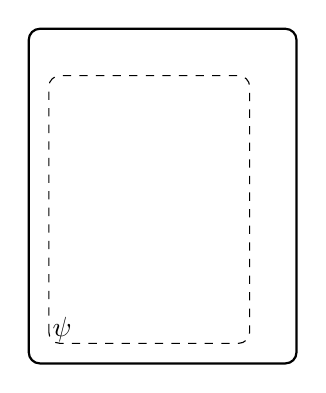
\begin{tikzpicture}[scale=.85]
      \coordinate (epVC) at (0,0);
      \coordinate (epV) at (4,5);
      \coordinate (epVLL) at ($(epVC)-0.5*(epV)$);
      \coordinate (epVUR) at ($(epVC)+0.5*(epV)$);
      \draw[thick, rounded corners] (epVLL) rectangle (epVUR);

      \filldraw (0.5*-3,0.5*-4) node {\(\psi\)};
      \coordinate (psiC) at (-.2,-.2);
      \coordinate (psi) at (3,4);
      \coordinate (psiLL) at ($(psiC)-0.5*(psi)$);
      \coordinate (psiUR) at ($(psiC)+0.5*(psi)$);
      \draw[dashed, rounded corners] (psiLL) rectangle (psiUR);
    \end{tikzpicture}
    \caption{\ref{def:requ:crequ:strcture:psi-not-v}}
    \label{fig:crequ:psi}
  \end{subfigure}
  \hfill
  \begin{subfigure}{0.3\linewidth}
    \begin{tikzpicture}[scale=.85]
      \coordinate (epVC) at (0,0);
      \coordinate (epV) at (4,5);
      \coordinate (epVLL) at ($(epVC)-0.5*(epV)$);
      \coordinate (epVUR) at ($(epVC)+0.5*(epV)$);
      \draw[thick, rounded corners] (epVLL) rectangle (epVUR);

      \filldraw (0,0) node {\(\phi\)};
      \coordinate (phiC) at (-.25,-.25);
      \coordinate (phi) at (2,3);
      \coordinate (phiLL) at ($(phiC)-0.5*(phi)$);
      \coordinate (phiUR) at ($(phiC)+0.5*(psi)$);
      \draw[dashdotted, rounded corners] (phiLL) rectangle (phiUR);

      \filldraw (0.5*-3,0.5*-4) node {\(\psi\)};
      \coordinate (psiC) at (-.2,-.2);
      \coordinate (psi) at (3,4);
      \coordinate (psiLL) at ($(psiC)-0.5*(psi)$);
      \coordinate (psiUR) at ($(psiC)+0.5*(psi)$);
      \draw[dashed, rounded corners] (psiLL) rectangle (psiUR);
    \end{tikzpicture}
    \caption{\ref{def:requ:crequ:strcture:subset} \& \ref{def:requ:crequ:strcture:propersubset}}
    \label{fig:crequ:subset}
  \end{subfigure}
  \hfill
  \begin{subfigure}{0.3\linewidth}
    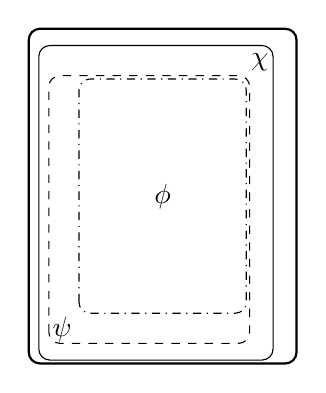
\begin{tikzpicture}[scale=.85]
      \coordinate (epVC) at (0,0);
      \coordinate (epV) at (4,5);
      \coordinate (epVLL) at ($(epVC)-0.5*(epV)$);
      \coordinate (epVUR) at ($(epVC)+0.5*(epV)$);
      \draw[thick, rounded corners] (epVLL) rectangle (epVUR);

      \filldraw (0.5*2.9,0.5*4) node {\(\chi\)};
      \coordinate (chiC) at (-.1,-.1);
      \coordinate (chi) at (3.5,4.7);
      \coordinate (chiLL) at ($(chiC)-0.5*(chi)$);
      \coordinate (chiUR) at ($(chiC)+0.5*(chi)$);
      \draw[rounded corners] (chiLL) rectangle (chiUR);

      \filldraw (0.5*-3,0.5*-4) node {\(\psi\)};
      \coordinate (psiC) at (-.2,-.2);
      \coordinate (psi) at (3,4);
      \coordinate (psiLL) at ($(psiC)-0.5*(psi)$);
      \coordinate (psiUR) at ($(psiC)+0.5*(psi)$);
      \draw[dashed, rounded corners] (psiLL) rectangle (psiUR);

      \filldraw (0,0) node {\(\phi\)};
      \coordinate (phiC) at (-.25,-.25);
      \coordinate (phi) at (2,3);
      \coordinate (phiLL) at ($(phiC)-0.5*(phi)$);
      \coordinate (phiUR) at ($(phiC)+0.5*(psi)$);
      \draw[dashdotted, rounded corners] (phiLL) rectangle (phiUR);
    \end{tikzpicture}
    \caption{Example premise(s)}
    \label{fig:crequ:intuition:prem-ex}
  \end{subfigure}
  \hfill\mbox{ }
  \caption{\crequ{}}
  \label{fig:crequ:intuition}
\end{figure}

\begin{note}[Weaker]
  That \(\psi\) having value \(v'\) is strictly weaker than \(\phi\) having value \(v\) captures an intuitive sense in which whether \(\psi\) has value \(v'\) is an antecedent check on concluding \(\phi\) has value \(v\) from \(\delta\).

  Further, \(\psi\) having value \(v'\) is strictly weaker than \(\phi\) having value \(v\) ensures that the definition of a \crequ{} is compatible with granting that concluding any proposition-value pair also \indicateV{} any weaker proposition-value pair.

  For, if \(\phi\) were to have value \(v\) in every \epVW{} for which \(\psi\) has value \(v'\) it would not be possible for the agent to conclude \(\psi\) has value \(v'\) without the conclusion also \indicateV{} \(\phi\) has value \(v\).\nolinebreak
  \footnote{
    Note, \ref{def:requ:crequ:strcture:psi-not-v} does not place any constraints on how the premises of the step of reasoning relate to \(\psi\) having value \(v'\) (or \(\phi\) having value \(v\)).
    \autoref{fig:crequ:intuition:prem-ex} depicts a possibility, but in general the agent may entertain arbitrary proposition-value pairs as premises.

    Hence, satisfying the definition of a \crequ{} will not ensure that the step is `reasonable'.
    For example, be that there is no \epVW{} where \(\chi_{1},\dots,\chi_{k}\) all have values \(v_{1},\dots,v_{k}\), and hence the agent would, if they were to conclude \(\phi\) has value \(v\), reason from premise proposition-value pairs that the agent do not consider \epVAd{}.

    Still, \ideaCS{} is only a necessary condition on claiming support, and in turn a \requ{}, and specifically a \crequ{}, need not capture every way in which a step of reasoning may be problematic (with respect to claiming support).

    And, as we will observe, the partner definition of a \prequ{} will place some constraints on when an agent may appeal to some premises to claim support for some conclusion.
  }

  It also follows from both \(\psi\) having value \(v'\) is strictly weaker than \(\phi\) having value \(v\) and the \epVN{} of \(\psi\) not having value \(v'\), that there is some \epVW{} in which \(\phi\) does not have value \(v\).
  In this respect, the definition of a \crequ{} is restricted to non-deductive steps of reasoning.\nolinebreak
  \footnote{
    This is not to deny that the definition of a \requ{} may be extended to cover cases of deductive reasoning.
    Still, it is unclear to me (at least) how the intuitive idea of a \crequ{} \emph{could} be extended to deductive steps.
    For, at issue is whether the agent may have first witnessed some other reasoning which would prevent the agent from concluding \(\phi\) has value \(v\), but if \(\phi\) having value \(v\) follows deductively, then no other reasoning is possible without the agent having concluded that some proposition has multiple incompatible values, or the agent revising their current epistemic state.

    Still, this is not to deny that an agent may make a non-deductive step of reasoning by appeal to a deductive step.
    For example, the agent may fail to note a key restriction on a theorem before applying it to a specific case.
    However, the distinction between whether a step of reasoning is deductive or non-deductive is made independently of the agent's perspective.
  }
\end{note}

\subsubparagraph{Relevance}

\begin{note}[Relevance]
  By relativising the core of the constraint to the agent's perspective we ensure that whether or not \(\psi\) has value \(v'\) is relevant to the agent's own reasoning.
  In particular, we ensure that whether or not \(\psi\) having value \(v'\) matters to whether or not \(\chi_{i}\) have values \(v_{i}\) by the agent's own lights, so to speak.

  Variations on the idea of a \prequ{} may take into account the epistemic states of other agents. For example if the agent were engaged in not merely reasoning to, but arguing for, some conclusion.
  Still, for present purposes we only identifying \(\psi\) having value \(v'\) as a \prequ{} if the agent considers it \epVAd{} to `check' their appeal to some premises prior to making a step of reasoning.

  This observation will be important for motivating \ideaCS{} via \ideaS{}.

  For now, observe:

  If \ref{def:requ:prequ:possible-reason} is satisfied, and the agent were to fail to conclude \(\psi\) has value \(v'\), then the agent would be unable to distinguish an \epVW{} in which \(\psi\) has value \(v'\) and \(\chi_{i}\) have values \(v_{i}\) from an \epVW{} in which \(\psi\) does not have value \(v'\) and \(\chi_{i}\) does not have values \(v_{i}\).
  Hence, it would seem that from the agent's perspective that they have no basis for concluding \(\phi\) has value \(v\) by appeal to \(\chi_{i}\) having values \(v_{i}\).
\end{note}

\subsubparagraph{The possibility of reasoning}

\begin{note}
  \ref{prequ:int:reasoning} is primarily captured by \ref{def:requ:prequ:possible-reason}.
  However, \ref{def:requ:prequ:possible-reason} is significantly more complex than \ref{prequ:int:reasoning}.

  In order to clarify \ref{def:requ:prequ:possible-reason}, we break down the clause in to three important components, and will discuss each component in turn.
  The three important components are:
  \begin{itemize}
  \item
    First, the core of the constraint concerning reasoning.
  \item
    Second, a relativisation of the core of the constraint to what is \epVAd{} for the agent.
  \item
    Third, a restriction on the scope of the core of the constraint relative to what is \epVAd{} for the agent to \epVW{1} in which the premises are true.
  \end{itemize}
\end{note}

\subsubparagraph{The core constraint}

\begin{note}[Constraint]
  The constraint:
  \begin{quote}
    There is some temporal extension of any relevant \epVW{} in which the agent witnesses reasoning which concludes \(\psi\) has value \(v'\).
  \end{quote}

  Recall, any (relevant) \epVW{} is a candidate for the actual \world{}.
  And, by temporal extension we mean the progression of a \world{} up to some future point in time.

  So, at core, the constraint specifies that the agent has the opportunity to reason about whether \(\psi\) has value \(v'\), and if the agent were to reason about whether \(\psi\) has value \(v'\), the agent would conclude \(\psi\) has value \(v'\).

  Note, the core of the constraint only requires that there is \emph{some} temporal extension of any given \epVW{}.
  Hence, the core of the constraint does not require that the agent \emph{will} conclude \(\psi\) has value \(v'\).
\end{note}

\begin{note}[Delicacy]
  On the one hand it is simple to fail the core of the constraint.
  For, the core of constraint requires that the agent would not fail to conclude \(\psi\) has value \(v'\).
  On the other hand, it is difficult to fail the core constraint.
  For, the core constraint requires only that there is at least one instance in which the agent would not fail to conclude \(\psi\) has value \(v'\).

  To illustrate, consider two different kinds of uncertainty.

  On the one hand, and agent may be uncertain about whether they would conclude \(\psi\) has value \(v'\) due to, say, requiring some information that they may or may not be in a position to acquire.
  If so, then the agent will be unsure about whether there \emph{is} a temporal extension of the relevant \world{}.
  For, the existence of the required temporal extension will depend on whether the agent acquires the required information.
  Hence the core of the constraint will not be satisfied.

  Note, the relevant sense of the copula `is' concerns existence, rather than possibility, however the notion of existence is understood for temporal extensions.

  On the other hand, an agent may be uncertain about whether they really do have the opportunity to conclude \(\psi\) has value \(v'\) as any instance of reasoning may be interrupted.
  However, so long as there is no guarantee that the agent's reasoning would be interrupted, then the core of the constraint will be satisfied, even if it is highly unlikely that the agent would conclude the relevant reasoning.

  Somewhere between these two extremes is a more nuanced constraint.
  Still, in order to keep the complexity of the constraint (relatively) low, we will not add further conditions.
  In cases where the constraint is to simple to fail, then the definition of a \requ{} may be added to, as \(\psi\) having value \(v'\) being a \prequ{} is only a sufficient condition for \(\psi\) having value \(v'\) being a \requ{}.
  And, we will avoid applying the definition of \prequ{} in cases where the definition exceeds intuition.
\end{note}

\subsubparagraph{The role of the agent}

\begin{note}
  Our discussion of the core of the constraint focused on there being some temporal extension of the \world{} in which \vAgent{} witnesses reasoning which concludes \(\psi\) has value \(v'\).

  In general, whether or not the core of the constraint is satisfied by be evaluated independently of the agent's perspective on how the actual \world{} is.
  Still, we relativise the core of the constraint to the agent's perspective.

  The motivation is simple and has two (related) parts.
  \begin{itemize}
  \item
    First, we ensure \(\psi\) having value \(v'\) is relevant to the agent's reasoning.
  \item
    Second, we reduce latent issues concerning whether there is some temporal extension of a \world{} to an single source --- the agent.
  \end{itemize}
  We expand on both points in turn.
\end{note}

\subsubparagraph{Latent issues}

\begin{note}
  The upshot of resolving the relevant sense of possibility to the agent's epistemic state is that we avoid questions about whether it is possible for an agent to recognise that it is possible for them to conclude \(\psi\) has value \(v'\).
  For, if it is \epVAd{} for the agent to witness reasoning which concludes \(\psi\) has value \(v'\), then the agent holds that for every candidate for the actual \world{}, there is some extension of the candidate \world{} in which the agent witnesses the relevant reasoning.\nolinebreak
  \footnote{
    Note, this does not guarantee that the agent would witness reasoning which concludes \(\psi\) has value \(v'\) if the agent were to try, as we do not require that the actual \world{} is always an \epVW{}.
  }

  For example, it may be `possible' for the agent to conclude that the liquid in a glass is not poisoned prior to appealing to it being safe to drink in order to conclude that they should drink the liquid.

  In order to resolve whether it really is possible the agent to conclude that the liquid in a glass is not poisoned, we need only consider whether the agent considers it \epVAd{} that they may witness such reasoning.
  And, the answer may be negative as the agent expects dehydration to set in before concluding any such reasoning.
\end{note}

\begin{note}
  The upshot comes with a corresponding downshot.
  For, it may be possible (in the relevant intuitive sense) for the agent to witness reasoning which concludes \(\psi\) has value \(v'\) without the agent holding that it is \epVAd{} for them to so reason.

  For example, it may be possible (and quite straightforward) for an agent to check the boiler for a simple fault before appealing to the premises that it is broken in order to conclude that they should call for a repair.
  Yet, so long as the agent does not consider it \epVAd{} for them to check the boiler, any proposition-value pair captured a simple fault will not be a \prequ{}.
\end{note}

\subsubparagraph{Quantification}

\begin{note}
  Finally we turn restricting the scope of the core of the constraint to \epVW{1} in which all of the premises that the agent would appeal to when making the step of reasoning have the appropriate values.

  Key here is that the core of the constraint requires that there is some temporal extension of the relevant \epVW{1} in which the agent witnesses reasoning which concludes \(\psi\) \emph{has} value \(v'\).

  This gives rise to the following problem:
\end{note}

\begin{note}[Problem]
  In order for \(\psi\) having value \(v'\) to be a \crequ{} the agent must consider it \epVAd{} \(\psi\) does not have value \(v'\).
  Yet, if \(\psi\) does not have value \(v'\), then it may be the case that the agent would fail to conclude \(\psi\) has value \(v'\).\nolinebreak
  \footnote{
    In particular, whether \(\psi\) has value \(v'\) may be straightforwardly decidable for the agent, and hence if the agent were to reason about whether \(\psi\) has value \(v'\) and \(\psi\) does not have value \(v'\), then they agent would conclude \(\psi\) does not have value \(v'\).
  }
  In which case, the core of the constraint will fail to be satisfied.
\end{note}

\begin{note}[Solution]
  \color{red}
  Still, quantifying over \epVW{1} in which \(\phi\) has value \(v\) provides a motivated solution.

  For, we are only interested in the idea \(\psi\) having value \(v'\) being \crequ{} as a check on whether it would make sense for an agent to conclude \(\phi\) has value \(v\) from a collection of premises.
  Hence, in order for the \crequ{} to be a check of the relevant kind, we are only interested in cases where the agent would (`successfully') make the step.

  In other words, the agent is moving to \(\phi\), and so long as this would make sense, it says something about what the agent can do.
  It does not need to follow that the agent can reason to \(\psi\) in general.

  Therefore, we may restrict the interest in the possibility of concluding \(\psi\) has value \(v'\) to those \epVW{1} in which \(\phi\) has value \(v\).
\end{note}

\subsubsection{\crequ{3}???}

\begin{note}
    \color{red}
    Note, focus on what the actual world is is important for the second clause.
    If it doesn't matter what the actual world is, then it's hard to see why this would matter.

    `Possible' should be restricted in some way.
    This is also why recursive in the case of \support{} is useful.
    Though, also should state that it's reasoning, with no further information.

    \requ{} is split into two cases.

    \ref{def:requ:crequ} observes that the result of making the step is a conclusion that \(\phi\) has value \(v\) only if \(\psi\) has value \(v'\).
    Alternatively, a conclusion that \(\phi\) has value \(v\) \emph{given} that \(\psi\) has value \(v'\).

    \ref{def:requ:prequ} observes that the premises appealed to cover all \epVW{1} only if \(\psi\) has value \(v'\).
\end{note}

\begin{note}[Intuition for \ideaCS{}]
  \ideaCS{}.
  The notion of a \requ{} specifies how \(\psi\) not having value \(v'\) is involved with step.
  Required in order to make step.
  Then, the problem is that the step will only conclude \(\phi\) has value \(v\) with respect to a restriction of \world{1} which are \epVAd{} for the agent.
  The agent may conclude that \emph{if} \(\psi\) has value \(v'\), \emph{then} \(\phi\), but as \(\psi\) may not have value \(v'\), the agent may not conclude \(\phi\) has value \(v\) alone.

  In other words, if an agent is \committed{} to it being that case that some step of reasoning in informative about the actual \world{} \emph{just in case} some proposition \(\psi\) has value \(v\), then unless the agent has witnessed some reasoning which \indicateV{1} \(\psi\) has value \(v'\), then the step only applies to a restricted collection of \epVW{1}.
\end{note}

\begin{note}[Dynamics]
  Stated in this way, \ideaCS{} is perhaps intuitive.

  The delicate part of \ideaCS{} is dynamics.
  In the cases of interest, the agent has concluded \(\chi_{i}\) have values \(v_{i}''\) from some prior reasoning, which have satisfied claiming support.
  However, between concluding \(\chi_{i}\) have values \(v_{i}''\) and reasoning from \(\chi_{i}\) have values \(v_{i}''\) to \(\phi\) having value \(v\), \(\psi\) (not) having value \(v'\) is introduced as an \epVN{}.

  This is where \ideaCS{} will do significant work.
\end{note}

\begin{note}[Relying]
  First, a subtle, but important, distinction is that the reasoning must \emph{rely} on the relevant step.
  Intuitively, some instance of reasoning which concludes \(\phi\) has value \(v\) relies on a step of reasoning just in case the reasoning requires both the premises and conclusion of the step to actually have their respective values in order to conclude \(\phi\) has value \(v\).

  In other words, \ideaCS{} does not extend to steps made where the step is part of some hypothetical reasoning, such as reasoning by cases.
\end{note}

\begin{note}[Intuition for \requ{}]
  Key is \(\psi\) having value \(v'\) is required to make the step.

  ??, ensures \(\psi\) not having value \(v'\) is relevant to making the step.
  There is not requirement that agent reasons about arbitrary \epVAd{} propositions.
  With respect to \ideaCS{}, keep things simple.
  Though, when defining a \requ{} in ???, strengthen somewhat.

  ??, reduces issues concerning the step to premises and conclusion of the step.

  ??, expands with respect to the agent's epistemic state.
  The use of the term `\committed{}' is to surpass any form of recognition.
\end{note}

\begin{note}
  Of course, it may be that the agent has \support{}.
  However, the reasoning would performed would not be suitable.
  Hence, failure of \emph{claiming} \support{}.

  Following \ideaS{}, \(\phi\) having value \(v\) is not a \sink{} with respect to \epVW{1}.
  Alternatively, it is not clear that the agent concludes \(\phi\) has value \(v\).
\end{note}

\paragraph{\illu{3}}

\begin{note}
  Some \illu{1}.
  Three \illu{1}.
  In each, reasoning which fails to satisfy \ideaCS{}, then suggested reasoning that would satisfy.
\end{note}

\begin{note}
  Observe, however, that the intuitive problem is not that the agent has any reason(ing) to think that \nagent{11} is \emph{not} trustworthy when speaking on matters regarding their personal character.

  Rather, the intuitive problem is that the agent does not have any reason(ing) to think that \nagent{11} \emph{is} trustworthy when speaking on matters regarding their personal character.

  In particular, that that \nagent{11} is not trustworthy when speaking on matters regarding their personal character is simply a possibility.
  It may be the case that \nagent{11} is trustworthy.\nolinebreak
  \footnote{
    \color{red}
    It's not like this suggests that they are not trustworthy.
    Asking for directions.
    These are fine, but addition is not.
  }
\end{note}

\subsection{Limitations}
\label{sec:limitations}

\begin{note}
  Goal of this section is to argue that \ideaCS{} does not over-generate.
\end{note}

\begin{note}
  The basic point is that while \(\psi\) is a consequence of \(\phi\), it's also the case that \(\phi\) is stronger.
  And, that the agent doesn't need to establish something so strong.
\end{note}

\begin{note}
  The bag contains green balls.
  The bag does not contain any red balls.

  Well, possible to empty the bag.

  However, \crequ{} doesn't cover this case, because the latter is not strictly weaker than the former.
\end{note}

\begin{note}
  X has at least \(\$100\).
  Well, then, X has at least \(\$1\), etc.

  Here, something nested.
  Where, it's always possible to check something weaker.

  It's hard to think of a compelling case.
  Still, the structure should be clear.

  Now, this does not mean that it is not possible for an agent to conclude some intermediary without previous.
  For, what the agent appeals to for an intermediary may also cover previous.
  Saw with \(\$50\), and this \indicateV{} \(\$50 - x\).

  What matters is that there's some jump, and an antecedent check on whether that jump makes sense that the agent hasn't considered.
  Yet \(\$50\) clearly works for all previous checks.
\end{note}

\subsection{\prequ{3}}
\label{sec:prequ3}

\begin{note}
  Definition of a \requ{} focused on particular structure.
  However, only a sufficient condition.
  Here, we consider \prequ{}.
  Observe this places further constraints.
  However, stronger.
  Any \prequ{} is a \crequ{}.
  Note, however, vice-versa.
\end{note}

\paragraph{Definition}

\begin{definition}
  \label{def:requ:prequ}
  \(\psi\) having value \(v'\) is a \emph{\prequ{}} of \(\delta\) \emph{if and only if} the following conditions jointly hold:
  \begin{enumerate}[label=\arabic*., ref=\named{P\(\Re\):\arabic*}]
  \item
    \label{def:requ:prequ:strcture}
    The structure of the \vAgent{}' epistemic state is such that:
    \begin{enumerate}[label=\alph*., ref=\named{P\(\Re\):1\alph*}]
    \item
      \label{def:requ:prequ:strcture:psi-not-v}
      There is some \epVW{} such that:
      \begin{itemize}
      \item
        \(\psi\) does not have value \(v'\).
      \end{itemize}
    \item
      \label{def:requ:prequ:strcture:chi-subset-psi}
      There is no \epVW{} such that:
      \begin{itemize}
      \item
        \(\chi_{i}\) have value \(v_{i}\) and \(\psi\) does not have value \(v'\)
      \end{itemize}
    \item
      \label{def:requ:prequ:strcture:chi-propersubset-psi}
      There is some \epVW{} such that:
      \begin{itemize}
      \item
        \(\psi\) has value \(v'\) and some \(\chi_{i}\) does not have value \(v_{i}\).
      \end{itemize}
    \end{enumerate}
  \item
    \label{def:requ:prequ:no-revision}
    It is not the case that the agent would revise their epistemic state so that \ref{def:requ:prequ:strcture:chi-subset-psi} does not hold (in order to conclude \(\phi\) has value \(v\) from \(\delta\)).
  \item
    \label{def:requ:prequ:possible-reason}
    For all \epVW{} in which \(\chi_{i}\) have values \(v_{i}\), there is some temporal extension of the \world{} in which \vAgent{} witnesses reasoning which concludes \(\psi\) has value \(v'\).
  \end{enumerate}
\end{definition}

\paragraph{Idea}

\begin{note}
  Intuitively, \(\psi\) having value \(v'\) is a \prequ{} of some step of reasoning just in case:
  \begin{enumerate}[label=\arabic*., ref=(\arabic*)]
  \item
    \label{prequ:int:structure}
    \(\psi\) not having value \(v'\) is \epVAd{} and the relevant \emph{premise} proposition-value pairs of the step are paired only if \(\psi\) has value \(v'\), and
  \item
    \label{prequ:int:reasoning}
    It is possible, given the agent's epistemic state, for the agent to conclude \(\psi\) has value \(v'\) prior to making the step of reasoning.
  \end{enumerate}
\end{note}

\paragraph{The structure}

\begin{note}
  \ref{prequ:int:structure} is primarily captured by \ref{def:requ:prequ:strcture}, where:

  \ref{def:requ:prequ:strcture:psi-not-v} ensures that \(\psi\) may not have value \(v'\).
  And, \ref{def:requ:prequ:strcture:chi-subset-psi} together with \ref{def:requ:prequ:strcture:chi-propersubset-psi} ensure that the \world{1} in which the premise proposition-value pairs holds are a subset (from \ref{def:requ:prequ:strcture:chi-subset-psi}) and moreover a \emph{proper} subset (from \ref{def:requ:prequ:strcture:chi-propersubset-psi}) of the \world{1} in which \(\psi\) has value \(v'\).

  \begin{figure}
    \mbox{ }\hfill
    \begin{subfigure}{0.3\linewidth}
      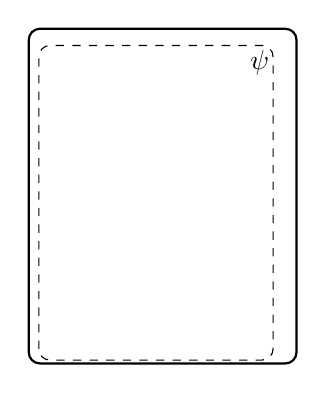
\begin{tikzpicture}[scale=.85]
        \coordinate (epVC) at (0,0);
        \coordinate (epV) at (4,5);
        \coordinate (epVLL) at ($(epVC)-0.5*(epV)$);
        \coordinate (epVUR) at ($(epVC)+0.5*(epV)$);
        \draw[thick, rounded corners] (epVLL) rectangle (epVUR);

        \filldraw (0.5*2.9,0.5*4) node {\(\psi\)};
        \coordinate (psiC) at (-.1,-.1);
        \coordinate (psi) at (3.5,4.7);
        \coordinate (psiLL) at ($(psiC)-0.5*(psi)$);
        \coordinate (psiUR) at ($(psiC)+0.5*(psi)$);
        \draw[dashed, rounded corners] (psiLL) rectangle (psiUR);
      \end{tikzpicture}
      \caption{\ref{def:requ:prequ:strcture:psi-not-v}}
      \label{fig:prequ:intuition:psi-not-v}
    \end{subfigure}
    \hfill
    \begin{subfigure}{0.3\linewidth}
      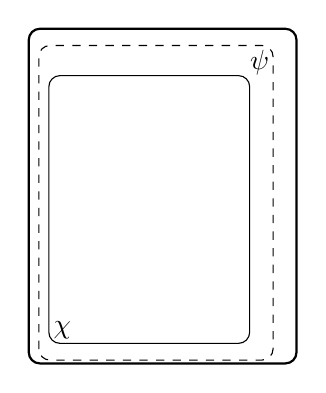
\begin{tikzpicture}[scale=.85]
        \coordinate (epVC) at (0,0);
        \coordinate (epV) at (4,5);
        \coordinate (epVLL) at ($(epVC)-0.5*(epV)$);
        \coordinate (epVUR) at ($(epVC)+0.5*(epV)$);
        \draw[thick, rounded corners] (epVLL) rectangle (epVUR);

        \filldraw (0.5*2.9,0.5*4) node {\(\psi\)};
        \coordinate (psiC) at (-.1,-.1);
        \coordinate (psi) at (3.5,4.7);
        \coordinate (psiLL) at ($(psiC)-0.5*(psi)$);
        \coordinate (psiUR) at ($(psiC)+0.5*(psi)$);
        \draw[dashed, rounded corners] (psiLL) rectangle (psiUR);

        \filldraw (0.5*-3,0.5*-4) node {\(\chi\)};
        \coordinate (chiC) at (-.2,-.2);
        \coordinate (chi) at (3,4);
        \coordinate (chiLL) at ($(chiC)-0.5*(chi)$);
        \coordinate (chiUR) at ($(chiC)+0.5*(chi)$);
        \draw[rounded corners] (chiLL) rectangle (chiUR);
      \end{tikzpicture}
      \caption{\ref{def:requ:prequ:strcture:chi-subset-psi} \& \ref{def:requ:prequ:strcture:chi-propersubset-psi}}
      \label{fig:prequ:intuition:subset}
    \end{subfigure}
    \hfill
    \begin{subfigure}{0.3\linewidth}
      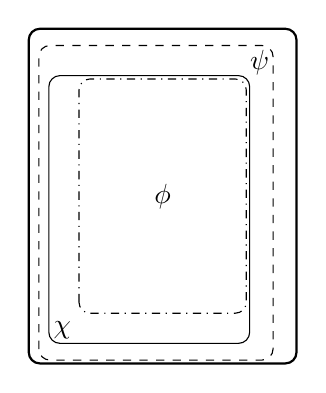
\begin{tikzpicture}[scale=.85]
        \coordinate (epVC) at (0,0);
        \coordinate (epV) at (4,5);
        \coordinate (epVLL) at ($(epVC)-0.5*(epV)$);
        \coordinate (epVUR) at ($(epVC)+0.5*(epV)$);
        \draw[thick, rounded corners] (epVLL) rectangle (epVUR);

        \filldraw (0.5*2.9,0.5*4) node {\(\psi\)};
        \coordinate (psiC) at (-.1,-.1);
        \coordinate (psi) at (3.5,4.7);
        \coordinate (psiLL) at ($(psiC)-0.5*(psi)$);
        \coordinate (psiUR) at ($(psiC)+0.5*(psi)$);
        \draw[dashed, rounded corners] (psiLL) rectangle (psiUR);

        \filldraw (0.5*-3,0.5*-4) node {\(\chi\)};
        \coordinate (chiC) at (-.2,-.2);
        \coordinate (chi) at (3,4);
        \coordinate (chiLL) at ($(chiC)-0.5*(chi)$);
        \coordinate (chiUR) at ($(chiC)+0.5*(chi)$);
        \draw[rounded corners] (chiLL) rectangle (chiUR);

        \filldraw (0,0) node {\(\phi\)};
        \coordinate (phiC) at (-.25,-.25);
        \coordinate (phi) at (2,3);
        \coordinate (phiLL) at ($(phiC)-0.5*(phi)$);
        \coordinate (phiUR) at ($(phiC)+0.5*(chi)$);
        \draw[dashdotted, rounded corners] (phiLL) rectangle (phiUR);
      \end{tikzpicture}
      \caption{Prospective conclusion}
      \label{fig:prequ:intuition:conclusion}
    \end{subfigure}
    \hfill\mbox{ }
    \caption{
      The structure of an agent's epistemic state with respect to \epVW{} when \ref{def:requ:prequ:strcture} is satisfied.
    }
    \label{fig:prequ:intuition}
  \end{figure}
  This structure is depicted in \autoref{fig:prequ:intuition}:

  \begin{itemize}
  \item
    \autoref{fig:prequ:intuition:psi-not-v} represents the agent's epistemic state (the bold rectangle) being such that there are some \world{1} such that \(\psi\) has value \(v'\) (those within the dashed rectangle), and that there are some \world{1} such that \(\psi\) does not have value \(v'\) (those outside the dashed rectangle).
  \item
    \autoref{fig:prequ:intuition:subset} represents the \world{1} in which the collection of premises \(\chi_{i}\) all have respective values \(v_{i}\) are a proper subset of the \world{1} such that \(\psi\) has value \(v'\).
  \item
    \autoref{fig:prequ:intuition:conclusion} represents a prospective conclusion, in which \(\phi\) having value \(v\) is obtained via a non-deductive step of reasoning from \(\chi_{i}\) having values \(v_{i}\), though the relevant step may also be deductive.
  \end{itemize}
\end{note}

\paragraph{\illu{3}}

\paragraph{Not completely trivial}

\begin{note}
  Trivially satisfied if the agent has concluded for each of the premises.
  For, given that \(\psi\) is strictly weaker than the premises, any reasoning for the premises is going to \indicateV{} \(\psi\).

  In this respect, fault is local to the reasoning, and again motivation for broadening to subjunctive considerations regarding relaxing and agent's epistemic state.

  Final: Not completely trivial.
  For, it may be the case that it is not possible for the agent to reason to one of the premises, but that \(\psi\) is still a condition that they could reason to.
\end{note}

\begin{note}
  \begin{illustration}
    The clock is working.
    Without any other source for the time, there's nothing to be done.
    However, it should definitely be ticking.
    Therefore, at the very least check this.
  \end{illustration}
  Or, that it's not clearly daylight outside.

  Not here that it's not clear that the clock would be particularly good.
  However, with respect to constraints, it's fine.
\end{note}

\subsubsection{Motivation}
\label{sec:motivation}

\begin{note}
  Provided clarification and some intuition.
  Seen some \illu{1}.
  Turn to motivation.

  Recap \ideaS{}, \support{}.
  Show how \ideaCS{} is motivated by \ideaS{}.
  Suggest that \ideaCS{} also motivates \ideaS{}.
\end{note}

\begin{note}
  First, this idea of claiming support is for how things are.
  If \epVW{}, then not for how things are.

  The difficulty is that we have no placed any constraints on reasoning.
  Specifically, steps of reasoning.
  Without preventing certain steps of reasoning, there is no problem with agent arbitrarily concluding that some proposition \(\phi\) has some value \(v\).

  Hence, \ideaS{} provided a partial constraint on the result of reasoning.
  We noted that this may still allow arbitrary reasoning, but \ideaS{} places some limits.
  Secures the conclusion with respect to the agent's epistemic state.
  What it is, in part, for the agent's reasoning to conclude something about how things are.
  Even if things were some other way, the agent would still reason to the relevant conclusion.
\end{note}

\begin{note}[Getting \ideaCS{} from \ideaS{}]
  Key property from \ideaS{} is that if an agent would not reason, then no \support{}.
  This is what matters.
  If agent fails to satisfy necessary condition of \ideaCS{}, then the reasoning would not be an instance of reasoning suitable for \support{}.

  For, suppose antecedent conditions.
  But, no reasoning.

  Then, given this, need \(\psi\) to have value \(v'\), but no reasoning which concludes \(\psi\) has value \(v'\).

  Now, this leaves open the possibility that if the agent were to reason about whether \(\psi\) has value \(v'\), then the agent would conclude \(\psi\) does not have value \(v'\).
  Indeed, \(\psi\) not having value \(v'\) may be a \sink{} with respect to the agent's epistemic state.
  Recall, the idea is that if the agent were to reason about\dots

  So, this means that the agent has no guarantee \(\phi\) having value \(v\) is a sink.

  Hence, lacking that the agent would reason even if \(\psi\) does not have value \(v'\).

  Indeed, the key part of \ideaS{} is reasoning about \epVAd{} proposition-value pairs.
  Our interest with relaxing with respect to \ideaS{} was to provide somewhat clear account of why the agent's reasoning concludes.
  Still, relaxing is important because it means that even after making the step, the agent would not necessarily have \support{}.

  Of course, still problem of whether the agent has \support{} for current epistemic state.
  However, only a necessary condition.

  Still, so long as agent satisfies \ideaCS{} for all reasoning, then plausible support.
  This is the converse.
\end{note}

\begin{note}
  From empty epistemic state.
  Satisfy \ideaCS{}.
  Then, plausibly support.
  As, reasoning about any \requ{}.
  So, if the agent were to relax, they would repeat same reasoning.
  Nothing would be `overlooked'.
\end{note}

\begin{note}
  \color{red}
  For, the underlying issue is that if no motivation for \(\psi\) having value \(v'\), then no account of why the step of reasoning is about how things actually are, rather than what follows from a restriction of how things actually are.
  \(\psi\) not having value \(v'\) remains a candidate, and so long as this is the case, then concluding \(\xi\) has value \(v''\) is not a conclusion about what is the case.

  Hence, if every step of reasoning satisfies \ideaCS{} from \epPAd{} \world{}, and the reasoning for \(\psi\) having value \(v'\) is sufficient, then it seems \ideaS{} will also be satisfied.
\end{note}

\subsection{\FCS{}}
\label{sec:fcs-2}

\begin{note}
  \begin{restatable}[\FCS{0}  --- \FCS{}]{proposition}{propFCS}
    \label{prop:fcs}
    Suppose:

    \begin{enumerate}
    \item
      \(\psi\) having value \(v'\) is a \crequ{} of step \(\delta\) to \(\phi\) having value \(v\).
    \item
      \vAgent{} requires \(\phi\) having value \(v\) from step \(\delta\)
      in order for some instance of reasoning (other than mentioned) to \indicateN{} that reasoning for \(\psi\) having value \(v'\) without doing the reasoning.
    \end{enumerate}

    Then:
    \begin{enumerate}[resume]
    \item
      It is not possible for \vAgent{} to claim support for \(\phi\) having value \(v\) without witnessing the reasoning which concludes \(\psi\) has value \(v'\).
    \end{enumerate}
    \vspace{-\baselineskip}
  \end{restatable}

  Hence, so long as \(\phi\) having \(v\) persists, further reasoning that appeals to \(\phi\) having value \(v'\) as a premise is (also) not an instance of claiming support without witnessing reasoning mentioned in {\color{red} inclusion}.
\end{note}

% \subsubsection{Weakening}
% \label{sec:weakening}

% \begin{note}
%   With a \requ{} we have that \(\psi\) is strictly weaker.
%   However, may also think anything equal.
%   Consider the following \illu{1}:

%   \begin{illustration}
%     \label{illu:requ:import-export}
%     Suppose we have some \emph{non-deductive} conditional `\(\Rightarrow\)' and some either deductive or non-deductive conditional \(\rightarrow\) such that:
%     \begin{quote}
%       \(\phi \Rightarrow (\psi \rightarrow \xi)\) if and only if \((\phi \text{ and } \psi) \Rightarrow \xi\)
%     \end{quote}
%     And, suppose an agent's reasoning has the structure:
%     \begin{enumerate}
%     \item \(\phi\)
%     \item \(\phi \Rightarrow (\psi \Rightarrow \xi)\)
%     \item \(\psi \Rightarrow \xi\)
%     \end{enumerate}
%     Such that possible \(\phi \rightarrow (\psi \rightarrow \xi)\) is not the case.
%   \end{illustration}

%   Here, \((\phi \text{ and } \psi) \Rightarrow \xi\) is a \prequ{} of the step from 2 to 3.
%   For, if \(\phi \Rightarrow (\psi \Rightarrow \xi)\) then also \((\phi \text{ and } \psi) \Rightarrow \xi\).
%   Hence, if \((\phi \text{ and } \psi) \rightarrow \xi\) is not the case, then \(\phi \Rightarrow (\psi \Rightarrow \xi)\) is also not the case.
% \end{note}

% \begin{note}
%   In other words, the non-deductive conditional admits of import-export.\nolinebreak
%     \footnote{
%       For example, the material conditional, but not necessarily the natural language conditional expressed in certain `if \dots then \dots' constructions {\color{red}~\cite{McGee:1985tz}}.
%     }
%     Consider the following pair of conditionals from~\citeauthor{McGee:1985tz}:
%     \begin{quote}
%       \begin{enumerate}
%       \item
%         \label{McGee:1}
%         If Uncle Otto hadn't found gold but he had struck it rich, it would have been by finding silver.
%       \item
%         \label{McGee:2}
%         If Uncle Otto hadn't found gold, then if he had struck it rich, it would have been by finding silver.\nolinebreak
%         \mbox{}\hfill\mbox{(\citeyear[467]{McGee:1985tz})}
%       \end{enumerate}
%     \end{quote}

%     If the main conditional of both statements admits of import-export, then~\ref{McGee:1} and~\ref{McGee:2} share the value true, or share the value false.

%     Still, even if an agent is \committed{} to import-export, it is perhaps not so clear that they would conclude that \ref{McGee:1} is true if and only if they would conclude that \ref{McGee:2} is true.
%     Counterfactuals are

%     Well, different things to evaluate.
%     So, gold was the last chance, hence the latter is trivial.
%     However, the former, need to do some work to allow for this possibility, so Otto would have had to have given up the efforts early, and so it's not clear that it would have been silver.

%     Well, maybe IE doesn't hold.
%     On the other hand, if committed, then this suggests that one is bad.
%     The second, plausibly, as reasoned about a restricted set of possibilities.
%     Or, the former, because you really shouldn't be revising so much.\nolinebreak
%     \footnote{
%       It seems~\textcite{Mandelkern:2020tc} makes some suggestions along these lines\dots
%     }
% \end{note}

% \begin{note}[The difficulty]
%   This I think is really quite plausible.
%   The difficulty is that I appeal to \indicateV{}.
%   In this sense, there's no difference between two proposition-value pairs of equal strength.
%   So, in order to have this, we would need to relax this simplifying assumption.

%   Intuitively, a distinction between trivial and non-trivial.
%   Suggestion is that different reasoning for showing for or against.
%   But making this precise is somewhat difficult.
% \end{note}

% \hozline

%%% Local Variables:
%%% mode: latex
%%% TeX-master: "master"
%%% End:

\chapter{Two ideas}
\label{cha:reasoning-two-ideas}

\section{Claimed support and `use'}
\label{sec:claimed-support-use}

\begin{note}[Sufficient condition]
  We start with a sufficient condition for claiming support:

  \begin{restatable}[\USE{0} --- \USE{}]{idea}{ideaUSE}
    \label{prem:bP}
    \label{prop:USE}
    If agent appeals to premises such that premises are part of reasoning, then the instance of reasoning may be an instance of claiming support.
  \end{restatable}

  \USE{} expresses an intuitive idea.

  In short, an agent may claim support when there are premises available to the agent, and the agent explicitly draws on those premises to claim support for the conclusion.

  Main argument of the thesis is about what is necessary for claiming support.

  We express \USE{} as an idea, rather than as assumption as we will not require \USE{}.
\end{note}

\begin{note}
  Two \illu{1}
\end{note}

\begin{note}[Illustration of \USE{}]
  \begin{illustration}
    \label{ill:rectangle:basic}
    \mbox{}
    \vspace{-\baselineskip}
    \begin{enumerate}
    \item The length of this rectangle measures \(19\text{cm}\) and the breadth of this rectangle measures \(7\text{cm}\).
    \item So, the length of this rectangle is \(19\text{cm}\) and the breadth of this rectangle is \(7\text{cm}\).
    \item
      It is possible that my measuring device in inaccurate, but I purchased it from a reliable hardware store.
    \item
      To calculate the area of a rectangle, one multiples the length of the rectangle by breadth.
    \item
      \label{ill:rectangle:basic:reasoning}
      \(19\text{cm}\) multiplied by \(7\text{cm}\) is \(133\text{cm}^{2}\).
    \item
      So, the area of the rectangle is \(133\text{cm}^{2}\).
    \end{enumerate}
    \vspace{-\baselineskip}
  \end{illustration}
\end{note}

\begin{note}
  \begin{illustration}[Waiting for a shop to open]
    \label{ill:waiting-for-shop}
    \mbox{}
    \vspace{-\baselineskip}
    \begin{enumerate}
    \item The sign in the door says that the shop will open at 10a.
    \item So, the shop will open at 10a.
    \item\label{ill:waiting-for-shop:reasoning} Of course, the sign may not be accurate, but it looks as though the store is well kept, so even if the sign is inaccurate, it is sufficient to indicate that the shop will open at 10a.
    \item\label{ill:waiting-for-shop:current-time} It is currently 9:45a.
    \item If 30 minutes pass, it will be 10:15a.
    \item 10:15a is after 10a.
    \item\label{ill:waiting-for-shop:return} So, if I return in 30m, then the shop will be open.
    \end{enumerate}
    \vspace{-\baselineskip}
  \end{illustration}
\end{note}

\begin{note}
  Both \illu{1} involves reasoning that intuitively amounts to claiming support.
  In particular, the third step of each \illu{0} involves reasoning about \requ{1} --- that the measure is accurate, and that the sign in the shop is truthful.
  Important from the perspective of \USE{}, however, is that the reasoning of both \illu{1} does not appeal to any premises other than those which form part of the instance of reasoning.

  In \autoref{ill:waiting-for-shop}, the agent's reasoning explicitly includes premises concerning the length and breadth of a rectangle and a statement of how to calculate the area of a rectangle given the rectangle's length and breadth.
  And, in \autoref{ill:waiting-for-shop} the agent reasons through premises concerning when the shop will open, what time it currently is, and what the result of some interval of time passing would be.

  Of course, one may hold that some of the steps in \autoref{ill:waiting-for-shop} and \autoref{ill:waiting-for-shop} are redundant.
  For example, it may be possible for an agent may move directly from \ref{ill:waiting-for-shop:current-time} to \ref{ill:waiting-for-shop:return}.

  Or, conversely, that steps in \autoref{ill:waiting-for-shop} and \autoref{ill:waiting-for-shop} are omitted.
  For example, it may be that \ref{ill:rectangle:basic:reasoning} should be expanded to state the operation of abstracting from \(\text{cm}\), multiplying \(19\) by \(7\), and applying \(\text{cm}^{2}\) to \(133\).

  However you may wish to revise these \illu{1}, the motivation behind \USE{} is hopefully clear:
  If appealing to a collection of premises is sufficient for claiming support for some conclusion, then so long as \ideaS{} and \ideaCS{} hold with respect to the instance of reasoning, the agent will succeed in claiming support.
\end{note}

\begin{note}
  In addition, though the \illu{1} of {\color{red} some section} fail to be instances of claiming support, the failure is not due to the agent appealing to premises that are not part of their reasoning --- rather, the failure is due to agent failing to reason about some \requ{}.
\end{note}

\begin{note}
  Further, though other \illu{1} that involve are not necessarily instances of claiming support, a variant of \USE{} which replaces `claiming support' and ideas \ideaS{} and \ideaCS{} with some other attitude and constraints.
\end{note}

\begin{note}[`Use']
  `Use'
\end{note}

\section{Two (conflicting) ideas as to claiming support}
\label{sec:inter-with-claim}

\begin{note}
  In this section we introduce two propositions which characterise what we are arguing against and what we are arguing for.
  \ESU{0} and \EAS{0}, respectively.
  Argue against \ESU{} by cases involving ability.
  Argue for \EAS{} which outlines the way in which ability conflicts with \ESU{}.

  Start with introduction of \ESU{}.
  And, motivate with reference to literature on the basing relation and rationality as responding to reasons.

  Move to \EAS{}, clarify relation to \ESU{} and contrast to related principle argued for by \citeauthor{Moretti:2019wx}.
\end{note}

\subsection{\ESU{0} --- \ESU{}}
\label{sec:esu}

\begin{note}[Recap of \USE{}]
  Brief recap of \USE{}.
  Introduced the idea, and then expanded on the details.
\end{note}

\begin{note}[Focus]
  We will argue against:

  \targetESU*

  In other words, only an instance of claiming support \emph{only} if agent has used the premises that they appeal to.
\end{note}

\begin{note}
  \ESU{} is equivalent to the converse of~\USE{}:\nolinebreak
  \footnote{
    Let:
    \(\phi\) {\color{red}???????}


    Note the logical form of \USE{} is \((\phi \text{ and } \psi) \rightarrow \xi\), the logical form of \ESU{} is \(\xi \rightarrow \psi\), and the logical form of \autoref{idea:ESUasUSE} is \(\xi \rightarrow (\phi \text{ and } \psi)\).
    So, \autoref{idea:ESUasUSE} is the converse of \USE{}.

    To establish equivalence between \ESU{} and \autoref{idea:ESUasUSE} we break this down into two directions:

    First, the implication from \autoref{idea:ESUasUSE} to \ESU{} is immediate.
    For, \(\phi\) implies \(\xi\) whenever \(\phi\) implies \(\psi \text{ and } \xi\).

    However, the implication from \ESU{} to \autoref{idea:ESUasUSE} is a little more complex.
    If \(\xi\) implies \(\phi\) and \(\xi\) implies \(\psi\), then \(\xi\) implies \(\phi \text{ and } \psi\).
    \ESU{} immediately ensures \(\xi\) implies \(\psi\).
    And, to observe that \(\xi\) implies \(\phi\) observe that an instance of reasoning is an instance of claiming support only if \ideaS{} and \ideaCS{} hold.
  }

  \begin{restatable}[]{idea}{ideaESUasUSE}
    \label{idea:ESUasUSE}
    An instance of reasoning is an instance of claiming support, \emph{only if}, \ideaS{} and \ideaCS{} hold and agent appeals to premises such that premises are part of reasoning.
  \end{restatable}

\end{note}

\begin{note}
  \USE{} includes assumption that \ideaS{} and \ideaCS{} hold with respect to the relevant instance of reasoning.
  However, as \ESU{} expresses a necessary, rather than sufficient, condition on claiming support, such assumptions are optional.
\end{note}

\begin{note}
  Focus is with whether an agent is required to have \emph{used} something in order to appeal to that thing when claiming support.
  No fixed understanding of `use' is assumed in the statement of~\ESU{}, and we will offer some disambiguation below.
\end{note}

\begin{note}
  Broad motivation for \ESU{} is somewhat complex.
  At issue is not instances of straightforwardly problematic reasoning.

  To illustrate, consider variant of illustration provided for~\USE{}.

  A lucky guess that the area of the rectangle is \(133\text{cm}^{2}\) would not allow the agent to claim support that the area of the rectangle is \(133\text{cm}^{2}\).
  However, the luck guess is part of the agent's reasoning.
  So, failure comes down to \ideaS{} or \ideaCS{}.
  Plausibly \ideaCS{}.
\end{note}

\begin{note}[Illustration]
  One way to generalise is to view claiming support as an instance of basing.
  So, doesn't get to base on the dimensions of the rectangle, the agent's understanding of how to calculate the area of a rectangle, and the relevant mathematics.

  And, it seems the agent is not in a position to base their lucky guess in such a way because the agent did not reason from the dimensions of the rectangle, the agent's understanding of how to calculate the area of a rectangle, and the relevant mathematics

  I think this is a plausible variant.
  Argument will also go against such an idea.

  However, stick with reasoning.

  Still, variant of this.

  Moving to another agent, observe doing the work, get report.
  Easy to resist, by adding in additional premise.
  Still, no presupposing that this needs to be done.

  That the other agent performed the calculation.
  However, what the other agent appealed to when reasoning, the agent does not get to appeal to \emph{that}.

  If the agent has not performed the calculation, then the agent may not appeal to the use of the calculation when claiming support --- rather, the agent mentions that the calculation is true.\nolinebreak
  \footnote{
    Slight weakening of~\ESU{} may be made.
    So long as \emph{some} agent has performed the calculation.
    Argue against~\ESU{}, and the argument made will hold for this weakening.
  }
\end{note}

\begin{note}
  To illustrate, claim support that 173 is prime.
  It's possible that I did the prime factorisation, and possible that I took that representation to be part of the reason why I claim that 173 is prime.
  However, represented query of whether prime to wolfram alpha as justifying, and that's why I claimed support.
  So, definitely not from okay to appeal to the reasoning I have not witnessed.
  And, if infer that 173 is prime from claimed support that I have the ability to demonstrate that 173 is prime, the same issue.
\end{note}

\begin{note}
  Three brief notes on~\ESU{}:
\end{note}

\begin{note}
  First, the `has' in~\ESU{} only requires `at some point in the past'.
  Hence,~\ESU{} does not require the agent to reason from premises to conclusion each time the agent claims support for the conclusion.
  For example, if an agent proved the Deduction Theorem for propositional logic last week, then the agent would not be in conflict with~\ESU{} if they claimed support for the Deduction Theorem on the basis of the premises and reasoning they performed in the past.
\end{note}

\begin{note}
  Second, and following from the first,~\ESU{} will also hold for any stronger statement --- for example if `has' is read as `has just'.
  For example, requiring that the agent's memory of proving the Deduction Theorem allows the agent to claim support, rather than the premises and steps used in the past.
  The argument (stated below) denies that, given certain information, the agent needs witnesses any reasoning in order to claim support for the result of witnessing the reasoning.
\end{note}

\begin{note}
  Third, as~\ESU{} is about when an agent may \emph{claim} support, it is compatible with~\ESU{} to hold that the agent \emph{has} support --- regardless of whether the agent has witnessing the reasoning.
\end{note}



\subsubsection{Intuition}

\begin{note}[Intuition]
  \ESU{} seems quite plausible, at least to me.
  The proposition is a careful statement of an intuitive ideas:

  Whether or not an agent claims support is the result of the structure of the reasoning process, and if some premises or step is not used, then it is irrelevant to the structure of the process.
  Hence, the only premises and steps of interest when claiming support are those used in the reasoning process.

  Claiming support is the result of some process, and the result of an process is explained by the constituents of the process.\nolinebreak
  \footnote{
    Ah, the homonculus.

    Question about whether the agent is important.

    This gets difficult.

    Consider clocks.
    Clock does not keep track of time.
    Rather, mechanical system designed to change in constant with some passage of time. (Cf.\ \textcite{Smith:1988aa}.)

    Agent may be like this.
    Distinction is intentionality.
    When I go about keeping track of the time, I'm attempting (at least typically) to maintain reference to what the time is.
    Figure out a way to approximate a second, and that's what's happening.
    Approximation.
    If it is noted that I requarly sigh every minute, use this, but I wouldn't be keep tracking of time, though you may be using regularity to do so.
    So, in the former case, using understanding of time, while in the latter not doing so.
  }

  As~\ESU{} is restricted to an agent claiming support, things seem a little easier.
  Problems with interpretation, however.
  Transparency.
  Familiar, if debatable, \illu{0}.
  Freud.
  (Here, adjourning the meeting by saying something mistaken.)
\end{note}

\begin{note}[Analogy]
  By analogy, whether or not my mug of (once cold) coffee overheats in the microwave is the result of some process involving electromagnetic radiation.
  My desire that the mug of coffee does not overheat is not used as part of the process of heating the coffee, and so is irrelevant to the structure of the process.

  My desire may explain why the mug of coffee is taking part in a certain process, and an unused premise or step may explain why an agent performed so reasoning.
  Still, a premise or step must be used as part of the process of reasoning to stand in explanation for the result of reasoning.

  Press the analogy further: Reasoning is a causal process.
  And, any property of reasoning reduces to cause and effect.
  If premises or steps are not used, then those premises or steps stands outside the relevant causal trace, and may not be appealed to when accounting for some structural property of the conclusion of the instance of reasoning (here, that the agent claims support for the conclusion).
\end{note}

\subsubsection{\ESU{} from the literature}

\begin{note}
  Our goal is to motivate \ESU{}.
  Strictly speaking, \ESU{} is about instances of reasoning which amount to claiming support.
  However, we will motivate \ESU{} by accounts of what reasoning involves.

  In other words, motivate \ESU{} by considerations about reasoning, rather than considerations about claiming support.

  Two broad ideas.
  \begin{enumerate}
  \item Causal accounts of reasoning.
  \item Something like \citeauthor{Boghossian:2014aa}'s Taking Condition.
  \end{enumerate}

  We being with causation in \autoref{sec:motivating-ESU:causation}.
  Here, argue for entailment.
  Specifically, causal accounts of reasoning imply \ESU{} with respect to what the accounts classify as reasoning.

  Strength of this motivation is entailment and prevalence of causal accounts.

  However, weakness is causation alone does not distinguish reasoning from other activities.
  We being \autoref{sec:motivating-ESU:beyond-causation} by motivating the previous point.
  And, then consider how various proposals for what is distinctive about reasoning motivate \ESU{}.
  The strength of such motivation is that it follows from considerations about what is distinctive about reasoning.
  The weakness is that we will not necessarily obtain anything as strong as entailment.
  Indeed, there may be some interest as to whether the rejection of \ESU{} is compatible with the accounts of reasoning considered.
\end{note}

\begin{note}[Qualification]
  However, an important qualification.

  We haven't said much about what reasoning is.
  And, without fixing an account of what reasoning is, there is no guarantee that any given account of reasoning will strictly entail \ESU{}.
  For, it may be that `reasoning' as mentioned in \ESU{} has broader scope than `reasoning' as mentioned in some theory of reasoning cited in motivation for \ESU{}, or conversely.
  In other words, only entailment if equivocation, and I do not wish to suggest that `reasoning' should be equivocated.

  Still, to the extent that \ESU{} and each account of reasoning concern some phenomena, and that each account of reasoning \emph{at least} concerns a phenomena closely related to the other accounts of reasoning, we suggest motivation for \ESU{} from closely related phenomena should motivate \ESU{}.\nolinebreak
  \footnote{
    One may think this is overly cautious.
    So, let me expand a little with reference to causal accounts of reasoning.

    The overall goal is to provide an argument against \ESU{}.
    If a causal account of reasoning implies \ESU{}, then the argument against \ESU{} will also be an argument against a causal account of reasoning.
    However, the argument relies on there being certain instances of reasoning that motivate rejecting \ESU{}.
    And, while one may reject that such purported instances of reasoning really are reasoning, one may also reject that such purported instances of reasoning are instances of reasoning to which one's favoured causal account applies.
    Hence, a rejection of \ESU{} may be compatible with a causal account of reasoning to the extent that \ESU{} fails for a broader sense of `reasoning'.

    Indeed, causal accounts of reasoning may distinguish an important part of a broader phenomena, and therefore it may be that rejecting \ESU{} (and hence causation) should merely amount to limiting the scope of such accounts.
  }
\end{note}

\paragraph{Causation}
\label{sec:motivating-ESU:causation}

\begin{note}
  We start with the easy case of causation.
  Motivation is simple.
  A causal account of reasoning implies \ESU{}.

  Causal accounts of reasoning are common.
  So, such causal accounts of reasoning imply \ESU{} with respect to what the accounts classify as reasoning.

  Note the somewhat cautious phrasing.
\end{note}

\begin{note}
  We being with~\cite{Armstrong:1968vh}.
  \begin{quote}
    We are not concerned here with logicians' questions about inference, but solely with the psychological process of inferring.
    The primary sense of the word is that in which it involves acquiring a belief on the basis of a belief already held.

    \mbox{}\hfill\(\vdots\)\hfill\mbox{}

    \dots to say that A infers \emph{p} from \emph{q} is simply to say that A's believing \emph{q} \emph{causes} him to acquire the belief \emph{p}.
    And the sense of `cause' employed here is the common or billiardball sense of `cause', whatever that sense is.\nolinebreak
    \mbox{}\hfill\mbox{(\citeyear[194]{Armstrong:1968vh})}
  \end{quote}
  \cite{Armstrong:1968vh} goes on to consider some issues, but these reflect the `simplicity' of saying that inference is a matter of causation between beliefs, rather than causation.
  `With these qualifications, it seems that our causal account of inferring can stand.'
  (\citeyear[197]{Armstrong:1968vh})

  Of course, \citeauthor{Armstrong:1968vh} talks about `inference' rather than `reasoning', and in doing so restricts the scope of the proposal from arbitrary ways in which a proposition may be evaluated.

  However, restricted implies \ESU{}.
  For, cause, then part.
\end{note}

\begin{note}
  The following two passages from \citeauthor{Wedgwood:2006ui} and \citeauthor{Broome:2013aa} (respectively) explicitly cast reasoning as a causal process:

  \begin{quote}
    Reasoning is a causal process, in which one mental event (say, one's accepting the conclusion of a certain argument) is caused by an antecedent mental event (say, one's considering the premises of the argument).\nolinebreak
    \mbox{}\hfill\mbox{(\cite[660]{Wedgwood:2006ui})}
  \end{quote}

  \begin{quote}
    So far as I can see, then, no further conditions need be added.
    I have arrived at necessary and sufficient conditions for a process to be active reasoning.
    Active reasoning is a particular sort of process by which conscious premise-attitudes cause you to acquire a conclusion-attitude.
    The process is that you operate on the contents of your premise-attitudes following a rule, to construct the conclusion, which is the content of a new attitude of yours that you acquire in the process.\nolinebreak
    \mbox{}\hfill\mbox{(\cite[234]{Broome:2013aa})}
  \end{quote}
  As we appealed to nothing other than causation when arguing that (a restricted form) \ESU{} follows from \citeauthor{Armstrong:1968vh} account of inference, the same considerations apply to both \citeauthor{Wedgwood:2006ui} and \citeauthor{Broome:2013aa}'s account of reasoning.
\end{note}

\begin{note}
  Finally, consider the following passage from \citeauthor{Boghossian:2014aa}:
  \begin{quote}
    \dots the property of a person’s thinking something \emph{for a reason} is not response-dependent.
    To say that R was S's reason for A'ing implies that S took R to support his A'ing at the time that he A'ed, and that his so taking it led to his A'ing.

    I don't see how S's being disposed to \emph{say} that R was his reason for A'ing could \emph{make it the case} that he took R to support his A'ing and that this taking had a certain causal impact.
    His saying it might be very good evidence that R was his reason.
    But saying that R was his reason can’t be \emph{constitutive} of R's being his reason.
    Causation is part of the idea of R's being his reason---and causation can't be a response-dependent property.\nolinebreak
    \mbox{}\hfill\mbox{(\citeyear[10--11]{Boghossian:2014aa})}
  \end{quote}
  \citeauthor{Boghossian:2014aa} is here arguing against dispositional accounts of the Taking Condition (which we will highlight shortly).
  However, in contrast to the previous citations \citeauthor{Boghossian:2014aa} appeals not the process of reasoning\nolinebreak
  \footnote{
    Or, strictly speaking, inferring in \citeauthor{Boghossian:2014aa}'s case.
  }
  but of what it is for some to think of something for a reason.
  Following \citeauthor{Boghossian:2014aa}, appealing to some proposition \(\phi\) as a reason for \emph{V}ing that \(\psi\) implies that there was some event in which the agent appeal to \(\phi\) in order to \emph{V} that \(\psi\).
  Granting that such event is an instance of reasoning, then \(\phi\) must have had some causal impact, and to have such causal impact it seems \(\phi\) must have been part of the instance of reasoning.
\end{note}

\begin{note}
  Causation is necessary.
  So, any instance of appealing is an instance of causation.
  Hence, premise is part of agent's reasoning.
  For, if not part, then no causation.
  No way for something that is not a part to cause.

  So, implication from causation to \ESU{}.

  At best, the appeal itself has causal role.

  Possible to read causation so that rejecting \ESU{} does not require rejecting causation.
  For, it may be case that agent appeals, but still has some causal role.
  Think of the testimony cases.
  Appeal to the content.
  Possible to state that there is some causal relation.
  However, distinct from proposals considered.
  And, have not found any proposal of this kind in the literature.

  Converse does not hold.
  Need not think that being part implies causal role.
  {\color{red} this is further grouping}.
\end{note}

\paragraph{Beyond causation}
\label{sec:motivating-ESU:beyond-causation}

\begin{note}
  Causation implies \ESU{}.
  However, question the role of causation.
\end{note}

\begin{note}
  \begin{quote}
    ``Plenty of blank leaves, I see!'' the Tortoise cheerily remarked.
    ``We shall need them \emph{all}!''
    (Achilles shuddered.)
    ``Now write as I dictate:---

    \begin{enumerate}[label=(\emph{\Alph*})]
    \item Things that arc equal to the same are equal to each other.
    \item The two sides of this Triangle are things that are equal to the same.
    \item If \emph{A} and \emph{B} are true, \emph{Z} must be true.
      \setcounter{enumi}{25}
    \item The two sides of this Triangle are equal to each other.''
    \end{enumerate}

    ``You should call it \emph{D}, not \emph{Z},'' said Achilles.
    ``It comes \emph{next} to the other three.
    If you accept \emph{A} and \emph{B} and \emph{C}, you \emph{must} accept Z.''

    ``And why \emph{must} I?''

    ``Because it follows \emph{logically} from them.
    If A and B and C are true, Z \emph{must} be true.
    You don't dispute \emph{that}, I imagine?''

    ``If \emph{A} and \emph{B} and \emph{C} are true, \emph{Z} \emph{must} be true,'' the Tortoise thoughtfully repeated.
    ``That's \emph{another} Hypothetical, isn't it?
    And, if I failed to see its truth, I might accept \emph{A} and \emph{B} and \emph{C}, and \emph{still} not accept \emph{Z}, mightn't I ?''

    \mbox{}\hfill\(\vdots\)\hfill\mbox{}

    ``Then Logic would take you by the throat, and force you to do it!''
    Achilles triumphantly replied. ``Logic would tell you 'You ca'n't help yourself.
    \dots''\nolinebreak
    \mbox{}\hfill\mbox{(\Citeyear[279--280]{Carroll:1895uj})}
  \end{quote}
  Achilles seems to be arguing that accepting \emph{A} and \emph{B} and \emph{C} would be sufficient.
  Tortoise denying that \emph{A} and \emph{B} and \emph{C} are sufficient.
  In particular, possible to accept \emph{A} and \emph{B} and \emph{C} without accepting \emph{Z}.

  Achilles is not citing a causal relation between [\emph{A} and \emph{B} and \emph{C}] and \emph{Z} (or, rather, \emph{D}).
  However, Achilles does seem to be citing a causal relation between accepting [\emph{A} and \emph{B} and \emph{C}] and accepting \emph{Z}.

  The Tortoise would violate some causal law.
  However, despair sets in as Achilles observes that the Tortoise is violating the proposed causal law, and hence it is no law at all.

  The issue is that though causation implies \ESU{}, have not motivated \ESU{} from perspective of whatever it is that distinguishes reasoning from any other process.
\end{note}

\begin{note}
  Consider \citeauthor{Boghossian:2014aa}'s Taking Condition:
  \begin{quote}
    (Taking Condition): Inferring necessarily involves the thinker \emph{taking} his premises to support his conclusion and drawing his conclusion because of that fact.\nolinebreak
    \mbox{}\hfill\mbox{(\Citeyear[5]{Boghossian:2014aa})}
  \end{quote}
  As with \citeauthor{Armstrong:1968vh}, inference --- and hence reasoning with beliefs --- rather than reasoning more broadly (\Citeyear[cf][2]{Boghossian:2014aa}).

  \begin{quote}
    The intuition behind the Taking Condition is that no causal process counts as inference, unless it consists in an attempt to arrive at a belief by figuring out what, in some suitably broad sense, is supported by other things one believes.

    In the relevant sense, reasoning is something we \emph{do}, not just something that happens to us.
    And it is something \emph{we} do, not just something that is done by sub-personal bits of us.
    And it is something that we do with an \emph{aim}---that of figuring out what follows or is supported by other things one believes.
    It’s hard to see how to respect these features of reasoning without something like the Taking Condition.\nolinebreak
    \mbox{}\hfill\mbox{(\Citeyear[5]{Boghossian:2014aa})}
  \end{quote}

  Though the Tortoise has accepted \emph{A} and \emph{B} and \emph{C}, the Tortoise has not \emph{taken} \emph{A} and \emph{B} and \emph{C} to support \emph{Z}.

  For \citeauthor{Boghossian:2014aa}, The Taking Condition expands on a causal process.
  There are various objections to the taking condition.\nolinebreak
  \footnote{
    See, for example,~\textcite{Hlobil:2014tq},~\textcite{Wright:2014tt}, and~\textcite{McHugh:2016vp}.

    \citeauthor{Hlobil:2014tq} argues against the Taking Condition as it distracts from what accounts of reasoning out to explain, rather than arguing against the Taking Condition directly.

    \citeauthor{Wright:2014tt} denies that reasoning must involve a state which connects premises to conclusions. (\citeyear[Cf.][33-34]{Wright:2014tt})

    And, \citeauthor{McHugh:2016vp} argue against the Taking Condition as the taking in question is that of \emph{support} between premises and conclusion.
  }

  Still, for our purposes the Taking Condition is simply a concise account of a necessary condition that distinguishes reasoning from other mental processes.

  And, while \citeauthor{Boghossian:2014aa} motivates the Taking Condition as a restriction on some causal process, the `because' present in the Taking Condition may be interpreted independently of causation.
\end{note}

\begin{note}
  Now, there is no immediate entailment from the Taking Condition (or something like it) to \ESU{}.
  For, without some account of what `taking' amounts to, we have merely fixed an adjective to capture some part of some phenomena.
  However, at issue is not whether the Taking Condition (or something like it) entails \ESU{}, but whether accepting the Taking Condition (or something like it) motivates \ESU{}.
  And, it seems plausible that the Taking Condition (or something like it) does.

  For, if



  However, important that the Taking Condition (or something like it) does not entail \ESU{}.
  For, plausible constraint on reasoning.
\end{note}

\begin{note}
  Two instances from the literature:
\end{note}

\begin{note}
  \citeauthor{Thomson:1965vv} suggests a doxastic variant of the Taking Condition, where are agent reasons from \(\phi\) to \(\psi\) just in case the agent believes that \(\phi\) is a reason for \(\psi\).
  \begin{quote}
    The claim which the 'formula' of p.\ 285\nolinebreak
    \footnote{
      The `formula' in question:
      \begin{quote}
    Now reasoning should surely involve drawing a conclusion from a set of premisses.
    But you can't be said to draw the conclusion that \emph{q} from \emph{p} if for all you know in knowing that \emph{p} it would at best be a matter of luck if \emph{q} as well.
    So to ``reason'' from \emph{p} by itself to \emph{q} isn't really to be reasoning; it's like saying one thing, and then taking a chance on it that something else is also true---like taking a leap in the dark, or more prosaically, like guessing.'
    (From here on I shall refer to this as the `\emph{formula}'.)\nolinebreak
    \mbox{}\hfill\mbox{(\citeyear[285]{Thomson:1965vv})}
  \end{quote}
}
    above was to support was this:
    suppose \emph{p} does not imply \emph{q}, and suppose a man says `\emph{p}, so \emph{q}';
    then he is not reasoning in saying this unless he believes that \emph{r}, where the conjunction of \emph{p} and \emph{r} implies \emph{q}, and \emph{r} is a suppressed premiss of his reasoning.\par
     But suppose such a man believes that \emph{p} is reason for \emph{q}; would this not be enough?
    `It would if ``\emph{p} is reason for \emph{q}'' were construed as a suppressed premiss of his argument'.
    Then let us so construe it.\newline
    \mbox{}\hfill\mbox{(\citeyear[294]{Thomson:1965vv})}
  \end{quote}
  Causation is absent from \citeauthor{Thomson:1965vv}.
  Does not imply that \citeauthor{Thomson:1965vv}'s proposal is independent of causation, but motivated does not appeal to causation.
\end{note}

\begin{note}
  And more recently \cite{Valaris:2014un} has argued for an explicitly non-causal doxastic account of the taking condition.

  \begin{quote}
    Explicitly reasoning from R to p just is, in part, believing that p follows from R.

    \mbox{}\hfill\(\vdots\)\hfill\mbox{}

    There is no suggestion that the belief that p follows from R plays a causal role in one’s reasoning from R to p, and so no room to wonder about how it could possibly play that role.\nolinebreak
    \mbox{}\hfill\mbox{(\citeyear[117--118]{Valaris:2014un})}
  \end{quote}
\end{note}

\begin{note}
  And \citeauthor{Wright:2014tt} offers a similar suggestion\dots

  For example, \citeauthor{Wright:2014tt}'s `Simple Proposal' may be substituted for the Taking Condition.
  \begin{quote}
    But consider instead the proposal, not that the status of the transition as inferential depends on the thinker’s judgments about his reasons, but that it depends on \emph{what his reasons are}.
    We want his acceptance of the premises to supply his \emph{actual} reasons for accepting the conclusion.

    \mbox{}\hfill\(\vdots\)\hfill\mbox{}

    Call this the Simple Proposal.
    It says that a thinker infers q from p\(_{1}\) \(\cdots\) p\(_{\text{n}}\) when he accepts each of p\(_{1}\) \(\cdots\) p\(_{\text{n}}\), moves to accept q, and does so for the reason that he accepts p\(_{1}\) \(\cdots\) p\(_{\text{n}}\).\newline
      \mbox{}\hfill\mbox{(\Citeyear[33]{Wright:2014tt})}
    \end{quote}

    However, \citeauthor{Wright:2014tt} denies that reasoning must involve a state which connects premises to conclusions and so however \citeauthor{Wright:2014tt}'s Simple Proposal is developed, it will not inolve a doxastic state:

    \begin{quote}
      What is needed, then, is an account of, or at least some insight into, what it is for certain intentional states of a thinker to be his actual reasons for his transition to another intentional state.

      [Which avoids] committing to the notion that doing something for certain reasons must involve a state that somehow registers those reasons as reasons for what one does.\nolinebreak
      \mbox{}\hfill\mbox{(\Citeyear[34]{Wright:2014tt})}
    \end{quote}
\end{note}

\begin{note}
  Question is whether this requires that premise is part of the agent's reasoning?
  Unlike causal, there is no simple argument.
  Details on what the representation amounts to.

  Still, if agent does not consider premise, then doubt that this is possible.
\end{note}

\paragraph{Correctly responding}

\begin{note}[Responding to reasons]
  As final motivation, consider the proposal at the core of \citeauthor{Lord:2018aa}'s (\Citeyear{Lord:2018aa}) thesis that being rational is to correctly respond to reasons.

  \begin{quote}
    \textbf{Correctly Responding:} What it is for A's \(\phi\)-ing to be ex post rational is for A to possess sufficient reason S to \(\phi\) and for A's \(\phi\)-ing to be a manifestation of knowledge about how to use S as sufficient reason to \(\phi\).\nolinebreak
    \mbox{}\hfill\mbox{(\Citeyear[143]{Lord:2018aa})}
  \end{quote}

  An agent's action is rational only if the action is a manifestation of some know-how.
  \citeauthor{Lord:2018aa} summaries:

  \begin{quote}
    \dots when one manifests one's know-how, dispositions that are directly sensitive to normative facts are manifesting. Thus, the competences involved in the relevant know-how make one directly sensitive to the normative facts\nolinebreak
    \mbox{}\hfill\mbox{(\Citeyear[16]{Lord:2018aa})}
  \end{quote}

  For our purposes, following example of manifesting know-how directly relates to reasoning:

  \begin{quote}
    The most salient disposition [when appealing to \emph{p} as a reason]\nolinebreak
    \footnote{Note, \citeauthor{Lord:2018aa} (explicitly) not talking about believing that \emph{p} is a reason, but argues that the cited disposition to present both when appealing to p as a reason and believing that \emph{p} is a reason.}
    is the disposition to (competently) use \emph{p} as a premise in reasoning.\nolinebreak
    \mbox{}\hfill\mbox{(\Citeyear[25]{Lord:2018aa})}
  \end{quote}

  Hence, suppose an agent appeals to a premise of reasoning in order to claim support for some conclusion.
  Then, if the agent does not use the premise of reasoning, it seems the agent does not manifest know-how, which is required for the appeal to meet \citeauthor{Lord:2018aa}'s account of rational action.

  Of course, that the noted disposition is the most salient does not rule out alternative, less noteworthy, dispositions.
  However, it is unclear to me how to \emph{manifest} know-how without use.
  Looking ahead, it does not seem to be the case that I manifest my ability to show that a certain rule of inference is sound when skipping over details in a completeness proof.
  However, I may manifest know-how regarding the (presumed) truth of the ability attribution.

  Likewise with my ability to establish a preference for tofu over any other kind of miso when ordering soup.
\end{note}

\begin{note}[Summarising illustrations]
  Stepping back,~\ESU{} may be seen as a desiderata for any account of claiming support.

  For:
  If an agent claims support for some conclusion of reasoning, then result of reasoning.
  So, premises.

  An adequate account of claiming support must explain how the premises used permit the agent to claim support.\nolinebreak
  \footnote{
    Note, however, that this argument does not imply that support for the conclusion must be accounted for in terms of the premises and steps used by the agent to claim support.
    As we will note below, one may hold that an enthymematic argument permits an agent to claim support, while the relevant relation of support is secured by the corresponding non-enthymematic argument.
    Cf.\ \textcite{Moretti:2019wx} for suggestions along these lines.
  }
  In turn, if an agent appeals to premises and steps that they did not use, then those premises and steps must be redundant.
\end{note}


\paragraph{Basing}

\begin{note}[Theories of basing]
  Connexion between \ESU{} and basing.
\end{note}

\begin{note}
  \citeauthor{Pollock:1999tm} introduce the basing relation with the following observation:
  \begin{quote}
    To be justified in believing something it is not sufficient merely to \emph{have} a good reason for believing it.
    One could have a good reason at one's disposal but never make the connection.
    \dots
    Surely, you are not justified in believing [something], despite the fact that you have impeccable reasons for it at your disposal.
    What is lacking is that you do not believe the conclusion on the basis of those reasons.\linebreak
    \mbox{}\hfill\mbox{(\Citeyear[35]{Pollock:1999tm})}
  \end{quote}
  The observation falls short of being an account of the basing relation, but the intuition \citeauthor{Pollock:1999tm} appeal to is instructive.
  It seems that an agent must connect reasons and the content of a belief in order for the belief to be formed on the basis of those reasons, and hence be justified by those reasons.
  In turn, if a connection is made between reasons and the content of belief, then those reasons are used by the agent.
\end{note}


\paragraph{Summary of motivation for \ESU{}}

\subsection{\EAS{0} --- \EAS{}}
\label{sec:eas}

\begin{note}
  Turning to ability.
  Suppose and agent appeals to
  \begin{enumerate*}
  \item their ability to demonstrate \(\phi\) is the case, and
  \item that \(\phi\) must be the case in order for the agent to have the ability to demonstrate that \(\phi\)
  \end{enumerate*}
  in order to claim support for \(\phi\).
  Then, the premises and steps involved in a full account of reasoning from the two claims must be sufficient to claim support that \(\phi\) is the case.
  So, as the agent does not witness their ability to demonstrate that \(\phi\) in such reasoning, it must be the case that claimed support for (the property of) having the ability to demonstrate that \(\phi\) is sufficient for such reasoning.
\end{note}


{
  \color{red}
  Perhaps include a note about how the argument relates to \EAS{}.
  I don't provide a direct argument, but this is the best way I see of resolving the tension.
}

\begin{note}[Alternative]
  \ESU{} is a universal claim, and so applies to all instances in which an agent may claim support for conclusion on basis of support for premises and steps of reasoning --- an agent may only claim support if the agent reasoned from the premises via the steps to the conclusion.

  Our goal is to motivate the following exception to \ESU{}:

  \goalEAS*
\end{note}

\begin{note}[Intuition for \EAS{}]
  \EAS{} is a conditional.
  Antecedent is claimed support for ability.
  Consequent is that it may be permissible to violate \ESU{}.
\end{note}

\begin{note}
  Now, started with \USE{}, and then looked at \ESU{}, the converse.
  Both of these we have a particular instance of reasoning in mind.
  Now, \EAS{} may, intuitively, be understood to states that whatever that reasoning is, if an agent has claimed support that they're able to witness such reasoning, then the agent may claim support.

  However, things are a little more complex.
  \EAS{} is about the ability to claim support to reason to some conclusion.
  However, \EAS{} does not state that the agent may claim support for the conclusion on the basis of the premises that they would reason from were they to witness the ability.

  Issue here is that the substance of \EAS{} --- what the relevant materia amounts to --- depends on two things:
  \begin{itemize}
  \item How (appeal to) ability is understood, and
  \item The kind of reasoning involved in the appeal to ability.
  \end{itemize}

  We will outline the basics, then reformulate \EAS{} using one what in which (appeal to) ability is understood.

  Start, how ability is understood.
  Lead naturally to the kind of reasoning involved.

  The argument for \EAS{} will not depend on how ability is understood, but the kind of reasoning involved.
  Still, kind of reasoning involved when combined with how ability is understood.
\end{note}

\begin{note}
  Briefly stated,
  \AR{} understands ability in terms of some (complex) property.
  \WR{} understands ability in terms of possible witnessing events.

  For example, \AR{} may involve the property (attribution) of understanding geometry, perhaps broken down into the understanding or availability of various definitions, propositions, lemmas, theorems, and steps of reasoning.
  While, \WR{} would involve reasoning with particular definitions, propositions, lemmas, theorems, and steps of reasoning.

  So, agent appeals to property, or the reasoning itself.

  The purpose of this distinction is to ensure that our argument against \ESU{} does not rest on a particular way of understanding ability that may not extend to other ways of understanding ability.

  Conjecture that these are fundamentally connected.
  Witnessing event only if understanding.
  And, understanding only if possible to witness reasoning.

  Still, difference.
  Relevant properties are properties of the agent as they are.
  The witnessing event, by contrast, is a possible event.\nolinebreak
  \footnote{
    Property of there being a possible event involving the agent.
    In this case, still distinct from \WR{} as that the agent is part of possible event is still distinct from the reasoning that the agent would witness in the relevant event.
  }

  These are brief characterisations, but enough for now.
  Both~\AR{}~and~\WR{} will be considered at length in~\autoref{sec:ar-wr-1}.
  In addition to a more thorough treatment of the core ideas, \autoref{sec:ar-wr-1} includes additional examples, and an argument that~\AR{}~and~\WR{} are exhaustive --- any way of understanding ability will conform to either~\AR{}~and~\WR{}.
\end{note}

\begin{note}
  Now turn to the kind of reasoning involved.

  Motivated \AR{} in terms of understanding of premises and steps of reasoning, and \WR{} in terms of a possible event in which agent reasons with particular premises and steps.

  However, a further distinction in terms of what appeal to the relevant premises and steps or instance of reasoning amounts to.

  First, there is the \emph{existence} of premises and steps, or the \emph{possibility} of the witnessing event.
  Second, there is the premises and steps themselves, or the witnessing event.

  Difference from perspective of step of reasoning.
\end{note}


\begin{note}[Types of reasoning]
  Consider proofs.

  \(p \lor q\)
  \(\lnot q\)
  \(p\)

  Premises alone do not establish \(p\).
  Combined they do.

  Claim support individually, then \(p\).
  Alone, these don't require \(p\).
  More in \autoref{sec:ability-ads-adc}.
\end{note}

\begin{note}[\EASw{}]
    \begin{restatable}[\EASw{0} --- \EASw{}]{thought}{thoughtEASw}\label{thought:EASw}
    If an agent has claimed support that they have the ability to (adequately) reason to some conclusion, then it may be permissible for the agent to claim support for the conclusion by claiming support for the premises and steps of reasoning that the agent would use to witness their ability to reason to the conclusion.
  \end{restatable}

  Loosely restated,~\EASw{} holds that if an agent may claim support for having the ability to witness some reasoning, and is aware of the conclusion of that reasoning, then the way in which the agent claims support for the conclusion of that reasoning may mirror the way in which the agent would claim support for the conclusion by witnessing the reasoning (and hence using the relevant premises and steps).
\end{note}

\begin{note}[Just an idea]
  \emph{Idea} as this is preferred way of thinking about ability.
  However, argument will not depend on this way of thinking.
\end{note}

\begin{note}
  The (possible) event of the agent witnessing their ability to demonstrate \(\phi\) involves reasoning with various premises and steps which culminate in claiming support for \(\phi\).
  So, if~\EASw{} is true, then the agent may appeal to those premises and steps which are used in the (possible) witnessing event.

  One way to think about~\EASw{} (which we will explore in more details later) is in terms of propositional support.
  For, if an agent has the ability to demonstrate that \(\phi\) is the case, then the agent has propositional support for \(\phi\) as there is a way for the agent to demonstrate that \(\phi\) is the case.
  In addition, that the agent has the ability to demonstrate that \(\phi\) is the case ensure that the agent is in a position to make use of the available propositional support for \(\phi\).
  In turn,~\EAS{} may be interpreted to hold that so long as the agent has such information about their position to make use of the available propositional support for \(\phi\) then the agent does not need to reason with the relevant propositional support in order to claim support for \(\phi\) in virtue of the available propositional support for \(\phi\).
\end{note}

\begin{note}[Conditional]
  Here, note that it's a conditional, but also that it only states there are instances.
  It doesn't follow that ability will always allow the agent to claim support.

  The conditional is weak primarily because it is not at all clear that it holds in general.
  There are various cases in which it seems appeal to ability is blocked.

  Easiest cases involve claiming support in some public setting.
  Of course, success in a public setting is not necessarily required for private success.
  Same problem with testimony.
  I'm confident in a source and you're not.
  I fail to convince you, but I remain convinced myself.

  Still, seems as though similar considerations extend.
  For example, doing a PSET where I'm allowed to use theorems I've already proved.
  Have notes of what those theorems are.
  And, ability to prove them.
  Still, might refrains from using them until I've proven them once again.

  More could be said here, and it may be possible to argue for a stronger variant of \EAS{}.

  Even though it's weak, the condition is still interesting.
\end{note}


\begin{note}
  So, if~\EAS{} is true, then there are cases in which an agent is not required to reason from premises they may claim support for to some conclusion in order to obtain support for the conclusion on the basis the support the agent has for the premises.\nolinebreak
  \footnote{
    Stated~\EAS{} as an exception to~\ESU{}.
    And, we will argue that~\EAS{} is true.
    However, we will not argue that~\EAS{} \emph{is an exception} to~\ESU{}.
    To do so would require an argument that \ESU{} holds for other cases.
    Likewise, no argument that~\EAS{} is the only exception, as to do so would require argument that~\ESU{} holds for all other cases.
    Take~\ESU{} to be plausible, and suspect that there are few, if any, further exceptions, but~\EAS{} may stand independently on any further statements about claiming support.
  }
\end{note}

\begin{note}
  \color{red}
  I want to clarify \EAS{} a little.
  The use of `may' is problematic.
  It could be read as `it's always okay, but it's up to the agent'.
  Or, `it's possible, given appropriate context'.
  The latter is what I want, and is important for cases where doubts are plausibly raised about the ability.
\end{note}

\begin{note}[\EAS{} \illu{0}]
  To illustrate \EAS{}

  \begin{illustration}\label{ill:rectangle:ability}
    Suppose you provide me with novel information that:
    \begin{enumerate}[label=\emph{A}\arabic*., ref=(\emph{A}\arabic*), series=EAS_counter]
    \item\label{EAS:ex:box:if} If I have ability to calculate the area of a box, then I have the ability to demonstrate that a rectangle with dimensions \(19\text{cm}\) by \(7\text{cm}\) has area \(133\text{cm}^{2}\).
    \end{enumerate}
    The information is `novel' because I have not been previously informed (in any way) about the area of a rectangle with dimensions \(19\text{cm}\) by \(7\text{cm}\).

    Still, I am confident that:
    \begin{enumerate}[label=\emph{A}\arabic*., ref=(\emph{A}\arabic*), resume*=EAS_counter]
    \item\label{EAS:ex:box:gen} I have the ability to calculate the area of a rectangle.
    \end{enumerate}
    Therefore, from \ref{EAS:ex:box:if} as an instance of \ref{EAS:ex:box:gen}:
    \begin{enumerate}[label=\emph{A}\arabic*., ref=(\emph{A}\arabic*), resume*=EAS_counter]
    \item\label{EAS:ex:box:spec} I have the ability to demonstrate that a rectangle with dimensions \(19\text{cm}\) by \(7\text{cm}\) has area \(133\text{cm}^{2}\).
    \end{enumerate}
    From~\ref{EAS:ex:box:spec} it follows that:
    \begin{enumerate}[label=\emph{A}\arabic*., ref=(\emph{A}\arabic*), resume*=EAS_counter]
    \item\label{EAS:ex:box:fact} A rectangle with dimensions \(19\text{cm}\) by \(7\text{cm}\) has area \(133\text{cm}^{2}\).
    \end{enumerate}
  \end{illustration}

  \EAS{} holds that, when I claim support for~\ref{EAS:ex:box:fact}, I may appeal to dimensions and formula.

  For, if~\ref{EAS:ex:box:spec} is the case then it is possible for me to witness reasoning in which I demonstrate that~\ref{EAS:ex:box:fact} is the case, and it is the premises and steps of reasoning used in such reasoning that establishes~\ref{EAS:ex:box:fact} is the case.
  I have not used those steps and premises, as I have not witnessed the relevant ability, but may I appeal to those steps and premises regardless --- or so we will argue.

  There is an important subtlety here.
  {
    \color{red}
    Not appealing to either~\ref{EAS:ex:box:gen} or~\ref{EAS:ex:box:spec} to claim support for~\ref{EAS:ex:box:fact}.

    An alternative.
    Indirectly claim support for premises via claimed support for~\ref{EAS:ex:box:gen} and hence~\ref{EAS:ex:box:spec} via~\ref{EAS:ex:box:if}.
    However, argue that this would not amount to instance of claiming support.

    Indeed, argument also rules out~\ref{EAS:ex:box:spec} to~\ref{EAS:ex:box:fact}.
  }
\end{note}

\begin{note}[More detail]
  \color{details}
  I do not expect \EAS{} to be intuitive.
  Indeed, we are not interested in \EAS{} because it is a more-or-less intuitive principle which conflicts the intuitive \ESU{}.
  Rather, we are interested in \EAS{} primarily because \EAS{} is a consequence of tension arising from three things:

  \begin{enumerate}
  \item\label{incomp:tri:q:1} \ESU{}
  \item\label{incomp:tri:q:2} scenarios involving an agent reasoning with information about an their own ability,
  \item\label{incomp:tri:q:3} and a principle concerning when an agent is permitted to claim support
  \end{enumerate}

  To briefly expand on~\ref{incomp:tri:q:2} and~\ref{incomp:tri:q:3}:

  Information that one has some specific ability so long as one has some general ability --- such as the (specific) ability to show \(25^{\circ}\text{C} = 77^{\circ}\text{F}\) given the (general) ability to convert between Celsius and Fahrenheit.
  And, an agent is never permitted to claim support for proposition having a certain value if the agent requires the proposition to have value \emph{in order to} claim support.
  (As an instance, an agent is not permitted to claim support for the truth of a proposition if the agent requires the proposition to be true \emph{in order to} claim support that the proposition is true.)\nolinebreak
  \footnote{
    The emphasis on `in order to' is important.
    The instance of the principle does not state that an agent is not permitted to claim support for the truth of a proposition if the agent requires the proposition to be true when claiming support that the proposition is true.
    I plausibly require that \(2 + 2 = 4\) when I claim support that \(2 + 2 = 4\), and this does not prevent me from claiming support by simple arithmetic.
    However, it would be impermissible (or so we will argue) to claim support that \(2 + 2 = 4\) by reasoning that the calculator is functional only if \(2 + 2 = 4\), and as the calculator states \(2 + 2 = 4\) it is the case that \(2 + 2 = 4\).
  }
  The details matter, and we postpone detailing this argument to~\autoref{sec:broad-argum-overv}.

  In short, assuming the scenarios exist, there is tension between intuitive principles governing what an agent appeals to when reasoning and structural principles governing the relation between what the agent appeals to when reasoning.
\end{note}

\begin{note}
  For the moment we attempt to clarify \EAS{} to some degree.
  Three subsections follow:

  \begin{enumerate}
  \item We will outline alternative reasoning patterns from~\ref{EAS:ex:box:if} to~\ref{EAS:ex:box:fact}, clarify why we focus on a particular type of reasoning pattern, and examine some initial objections to~\EAS{} and canvas some responses.
  \item We will consider parallels between abilities and dispositions.
    The parallel will provide some additional intuition for why an agent may appeal to premises and steps that have no been used, and help further clarify our interest with ability.
  \item We will consider a related proposition argued for by \citeauthor{Moretti:2019wx} which holds that a belief need not be based (exclusively) on the premises and steps of reasoning used to arrive at the belief.
    The comparison will help highlight what is distinctive about~\EAS{} while at the same to introducing some ideas which suggest a way of understanding~\EAS{}.
  \end{enumerate}
\end{note}

\subsubsection{Against \EAS{}}

\begin{note}[Alternatives]
  The alternative reasoning pattern we will focus on in some detail holds that appealing to having the ability noted in \ref{EAS:ex:box:spec} is sufficient to claim support for \ref{EAS:ex:box:fact}.
  In line with \ESU{}, the agent would use the proposition that they have the relevant ability noted in~\ref{EAS:ex:box:spec} to claim support for~\ref{EAS:ex:box:fact}
  This reasoning pattern, along with the pattern suggested by \EAS{} will be considered in \autoref{sec:wr-ar} and we will argue that it conflicts with an intuitive principle regarding claiming support in \ref{sec:second-conditional}.

  Alternatively, on may argue that though the syntactic form of \ref{EAS:ex:box:if} is a conditional, it does not (necessarily) follow that the semantic content of~\ref{EAS:ex:box:if} is a (also) conditional.
  And that~\ref{EAS:ex:box:if} may (plausibly) be interpreted to explicitly state that~\ref{EAS:ex:box:spec} is an ability that an agent may have.
  For example:
  \begin{enumerate}[label=\emph{A}\arabic*., ref=(\emph{A}\arabic*), resume*=EAS_counter]
  \item\label{EAS:ex:box:if:R:state} The ability to demonstrate that a rectangle with dimensions \(19\text{cm}\) by \(7\text{cm}\) has area \(133\text{cm}^{2}\) is an ability an agent may have and it is an ability an agent has if they have ability to calculate the area of a rectangle.
  \end{enumerate}
  Hence, \ref{EAS:ex:box:if} is interpreted so that \ref{EAS:ex:box:spec} is accessible without endorsing the antecedent of \ref{EAS:ex:box:if}.
  \ref{EAS:ex:box:if:R:state} states that there is some ability that it is possible for an agent to have, and in addition provides sufficient conditions for having the relevant ability.
  The important part of \ref{EAS:ex:box:if:R:state} is the former conjunct:
  \begin{enumerate}[label=\emph{A}\arabic*., ref=(\emph{A}\arabic*), resume*=EAS_counter]
  \item\label{EAS:ex:box:spec:R:state} The ability to demonstrate that a rectangle with dimensions \(19\text{cm}\) by \(7\text{cm}\) has area \(133\text{cm}^{2}\) is an ability an agent may have.
  \end{enumerate}
  And, \ref{EAS:ex:box:fact} follows from \ref{EAS:ex:box:spec:R:state} by the observation that it is not possible to demonstrate \(\phi\) if \(\phi\) is not the case --- there is no need for the agent to appeal to witnessing their ability.
  Therefore,~\ref{EAS:ex:box:spec:R:state} (and~\ref{EAS:ex:box:if:R:state}) implicitly includes information that~\ref{EAS:ex:box:fact} is the case --- an agent does not need to reason from~\ref{EAS:ex:box:spec} to~\ref{EAS:ex:box:fact}, because they have already been informed that~\ref{EAS:ex:box:fact} is the case.

  Note also that analogous reasoning applies if `I' is replaced with `an agent'.
  Likewise, if I know that you that you know that I have the ability to calculate the area of a rectangle.
  For, it then follows that you know that \ref{EAS:ex:box:spec} is the case, and therefore you know that \ref{EAS:ex:box:fact} is the case.
  Again there is no need for me to appeal to witnessing an ability.
\end{note}

\begin{note}[Box]
  The existence of alternative reasoning patterns is the issue at hand.
  For, so long as there are reasoning patterns \emph{R} which conform to \ESU{} it is open to the defender of \ESU{} to hold that if an agent is permitted to claim support, then the agent is required to reason via some member of \emph{R}.
  For, if there are reasoning patterns \emph{R} which conform to \ESU{} then there a no counterexamples to \ESU{} --- scenarios in which an agent claims support by appeal to premises or steps of reasoning that the agent has not used.

  Of course, an argument against a general principle such as \ESU{} is not required to be a counterexample.
  For example, it may be possible to argue that the reasoning patterns \ESU{} requires are sufficiently implausible.
  Hence, a restricted variant of \ESU{} compatible with \EAS{} would to be preferred.
  However, there are two issues with attempting such an argument.

  First, given the intuitive plausibility to \ESU{}, it seems unlikely that any violation of \ESU{} would be more plausible than an alternative reasoning pattern compatible with \ESU{}.
  Second, even if there are plausible reasoning pattern that are incompatible with \ESU{}, it is not clear that these should be incorporated in a theory of claiming support.
  For, meta-theoretical issues such as complexity or predictive power may still favour \ESU{}.
  Following \citeauthor{Box:1987vn}: `\dots all models are wrong; the practical question is how wrong do they have to be to not be useful.' (\Citeyear[74]{Box:1987vn})

  Indeed, the second point suggest a counterexample proper to show that \ESU{} is false is not necessarily an adequate argument against \ESU{} either.
  Observations in the spirit of \citeauthor{Box:1987vn} are trite, but also true.
  Even if \EAS{} is true and \ESU{} is false, would \EAS{} be useful?
\end{note}

\begin{note}[Responding to Box]
  With respect to idealised agents with unbounded resources, the answer appears to be no.
  For, with unbounded resources the agent the option of (attempting to) witnessing any ability (to reason) without cost.
  And, it seems that for such an agent witnessing a relevant ability would always be preferable to reasoning about an unwitnessed ability as the agent would minimally (subjectively) resolve any uncertainty about whether they have the ability.

  However, for limited agents, ability is abundant, while the resources required to witness abilities are scarce.
  That the exception to~\ESU{} is narrow does not entail that there are few occurrences of the exception.

  Information about ability may be abundant while the resources for witnessing abilities are either scarce or temporarily unavailable.
  So, for example, agent has the option of conserving or deferring use of resources.

  This observation suggests an initial line of response to an objection which focuses on whether \EAS{} would be useful.

  For, given that we are resource bound agents, it seems that possible instances of \EAS{} are widespread.
  From a functional perspective, reasoning with (the relevant instances of) ability just is reasoning about the result of expending available resources.
  Hence, if~\EAS{} is true, then the truth of \EAS{} would provide a novel perspective on resource bound agents.
  And, it is yet to be seen whether such a perspective is useful.

  In addition, there is a second indirect line of response.
  We observed above that \ESU{} seems prevalent in various theories which relate to reasoning, such as basing and responding to reasons.
  If \EAS{} is true, then there may be alternative conclusions to arguments that appeal to~\ESU{} as a premise.
  And, likewise, there may be interesting observations made in premises of arguments which establish \ESU{} as a foundation for further theorising.\nolinebreak
  \footnote{
    As an exception, even if~\EAS{}, conclusion of arguments which appeal to or assume \ESU{} may be restricted.
  }
\end{note}

\begin{note}[Taking stock]
  Taking stock:
  I doubt that \EAS{} is of interest if there are no reasoning patterns which require \EAS{} to be true.
  Still, if there are reasoning patterns which require \EAS{} to be true, then \EAS{} may be of interest.
  Further, I think there are good reasons to hold that there are reasoning patterns which require \EAS{} to be true.
  Hence, my goal is to motivate further research into whether \EAS{} is of interest.
\end{note}

\paragraph{Type of scenario}

\begin{note}
  We now briefly turn to the type of scenarios which are a premise in our argument for the existence of such counterexamples.
\end{note}

\begin{note}[Types of scenario]
  The type of scenario we will focus on is designed to ensure that an agent is required to reason to (and from) information about a (specific) ability that they have.
  If the agent is required to reason \emph{to} (specific) ability information then rephrasing \ref{EAS:ex:box:if} as \ref{EAS:ex:box:if:R:state} will not be possible --- the agent will be required to reason from some premises by some steps to the (specific) ability information.
  And, as before, the type of scenario will preserve the requirement of the agent to reason \emph{from} the (specific) ability information in line with~\ref{EAS:ex:box:spec} and~\ref{EAS:ex:box:if:R:state}.
  Hence, by establishing such scenarios are possible we may restrict our attention to the steps from~\ref{EAS:ex:box:if} to~\ref{EAS:ex:box:spec} and from~\ref{EAS:ex:box:spec} to~\ref{EAS:ex:box:fact}.
\end{note}

\begin{note}
  To illustrate, let us add some context to the example scenario we've been focusing on.

  Suppose it is common knowledge between you and I that
  \begin{enumerate*}
  \item you have looked through my notes, and have applied my formula for calculating the area of a rectangle, and
  \item my notes are the only source of information you have regarding how to calculate the area of a rectangle.
  \end{enumerate*}
  We may now restate the semantic content of~\ref{EAS:ex:box:if} as follows:
  \begin{enumerate}[label=\emph{A}\arabic*., ref=(\emph{A}\arabic*), resume*=EAS_counter]
  \item\label{EAS:ex:box:inf:R} You have some general ability \(\gamma\), and a specific ability \(\varsigma\) (as an instance of that general ability).
    And, if \(\gamma\) is the ability to calculate the area of a rectangle, then \(\varsigma\) is the ability to demonstrate that a rectangle with dimensions \(19\text{cm}\) by \(7\text{cm}\) has area \(133\text{cm}^{2}\).
  \end{enumerate}
  The formula in my notes indicates that I have the ability to do something, and I have indicated what I think the appropriate characterisation of the ability is.
  Still, you are not in a position to offer information as to whether my characterisation of the ability is correct or not.\nolinebreak
  \footnote{
    Consider in reverse.
    One is often attributed abilities that I deny I have.
    For example, I do not have the ability to process information by means of mental images, but \citeauthor{Hume:2011aa} (arguably) holds that I do have such an ability.
    I lack the ability to reason in a particular way.
    (Not that \citeauthor{Hume:2011aa}'s arguments rest on visual as opposed to any other kind of imagination, but the point stands.)

    Similarly, you may claim that I have the ability to tell you whether or not \nagent{7} is coming to tea.
    However, and in contrast to your assumption, \nagent{7} has not replied to my invitation and so I lack a required premise in order to reason to a relevant conclusion.
  }
  The key feature of~\ref{EAS:ex:box:inf:R} it that I, the agent, am required to claim support that \(\gamma\) and \(\varsigma\) are the abilities of interest.
  The focus is not on whether or not an agent may perform some action.
  Rather, our interest is with what the action is.
  It is up to me, the agent, to claim support that:
  \begin{enumerate}[label=\emph{A}\arabic*., ref=(\emph{A}\arabic*), resume*=EAS_counter]
  \item\label{EAS:ex:box:gen:R} The general ability \(\gamma\) \emph{is} the ability to calculate the area of a rectangle.
  \end{enumerate}
  If so, I may then claim support that:
  \begin{enumerate}[label=\emph{A}\arabic*., ref=(\emph{A}\arabic*), resume*=EAS_counter]
  \item\label{EAS:ex:box:spec:R} \(\varsigma\) is the specific ability to demonstrate that a rectangle with dimensions \(19\text{cm}\) by \(7\text{cm}\) has area \(133\text{cm}^{2}\).
  \end{enumerate}
  Note, there is no route to \ref{EAS:ex:box:spec:R} other than by claiming support for~\ref{EAS:ex:box:gen:R} as I have no information about what the (specific) ability \(\varsigma\) is amounts to if \ref{EAS:ex:box:gen:R} is not the case.
  If \(\varsigma\) is some other ability, then~\ref{EAS:ex:box:fact} does not follow, witnessing the relevant ability would not demonstrate that a rectangle with
  dimensions \(19\text{cm}\) by \(7\text{cm}\) has area \(133\text{cm}^{2}\), and so a rectangle with dimensions \(19\text{cm}\) by \(7\text{cm}\) may (from my epistemic perspective) have some other area.
\end{note}

\begin{note}[Point]
  We will say more in \autoref{sec:cases-interest}.
  For the moment it is sufficient to observe that the agent is required to reason to and from specific ability.
  The scenario requires the agent to claim support by reasoning from~\ref{EAS:ex:box:if} to~\ref{EAS:ex:box:spec} and from~\ref{EAS:ex:box:spec}~to~\ref{EAS:ex:box:fact}.
  And, while the context added to force the reasoning pattern of interest is narrow, the principle behind the context is simple:
  The agent is required to claim support that they have the relevant general ability.
  Hence, any scenario which consists of \gsi{0} which requires the agent to claim support that they have the relevant general ability will require the same kind of reasoning pattern.
\end{note}

\begin{note}[Puzzle about ability]
  Further, this arguably captures a general puzzle about ability.
  An agent is not required to have witnessed all instances of a general ability to claim support that they have the general ability.
  However, so long as the agent may claim support for having some general ability, then it follows that the agent will have the option of claiming support for each instance of the general ability.

  The primary issue, though, is whether there is an account of such reasoning that does not require \EAS{} to be true.
  We will shortly turn to this argument in \autoref{sec:broad-argum-overv}.
  Prior to doing so, we close this section with some further clarification on the motivation behind \EAS{}, what distinguishes \EAS{} from nearby principles, and a suggestion on how to conceptualise \EAS{}.
\end{note}

\subsubsection{Ability and dispositions}

\begin{note}[Parallel]
  To further clarify the motivation for \EAS{} we introduce a parallel between abilities and dispositions.
  The primary function of the parallel will be to highlight the importance of reasoning about an event.
  In the case of dispositions the event is the manifestation of the disposition, and in the case of ability the event is the agent witnessing the ability.

  The parallel is of interest because \EAS{} concerns the premises and steps of reasoning that the agent would use to witness the relevant ability.
  We will suggest that claiming support that some object has some disposition and that some agent has some ability may both be understood in terms of claiming support that the relevant event is a possible event.

  In turn, if reasoning \emph{to} a specific ability is understood in terms of claiming support that it is possible for the agent to witness the event, then reasoning \emph{from} a specific ability may be understood in terms of claiming support from what would happen in the possible event.
  \end{note}

\begin{note}[Parallel between dispositions and ability]
  Consider \citeauthor{Choi:2021wg}'s characterisation of the Simple Conditional Analysis of dispositions:
  \begin{quote}
    An object is disposed to \emph{M} when \emph{C} iff it would \emph{M} if it were the case that \emph{C}.\nolinebreak
    \mbox{}\hfill\mbox{(\Citeyear{Choi:2021wg})}
  \end{quote}
  For example, an object is disposed to dissolve when it is placed in water iff the object would dissolve if it were the case that it is placed in water.

  The Simple Conditional Analysis may be challenged, but for our purposes it is adequate.
  We are interested in the broad form of the truth condition, and various more refined analyses share the same broad form.
  Note, in particular, that it being the case that \emph{C} and \emph{M} happening describes an event.
  Given appropriate conditions; salt dissolves, glass breaks, and I mumble when I am tired.
  The key idea is that the property of being disposed to \emph{M} when \emph{C} is analysed in terms of the (possible) event of \emph{M} happening when \emph{C}.

  The parallel to ability is established by noting that ability may also be analysed in terms of a (possible) event, as we have seen.
  In particular, by incorporating volition in the analysans of the Simple Conditional Analysis.
  To illustrate, \citeauthor{Mandelkern:2017aa} trace the Conditional Analysis of ability  to \textcite{Hume:1748tp} and \textcite{Moore:1912te}, among others:
  \begin{quote}
    S can \(\phi\) iff S would \(\phi\) if S tried to \(\phi\)\nolinebreak
    \mbox{}\hfill\mbox{(\Citeyear[Cf.][308]{Mandelkern:2017aa})}
  \end{quote}
  Compare to the Simple Conditional Analysis of dispositions:
  The object is some agent \emph{S}, \emph{C} is `S tried to \(\phi\)' and \emph{M} is `S \(\phi\)s' --- it is volition alone which distinguishes the analyses.
  For example, I have the ability to demonstrate that a rectangle with dimensions \(19\text{cm}\) by \(7\text{cm}\) has area \(133\text{cm}^{2}\) only if I would demonstrate that a rectangle with dimensions \(19\text{cm}\) by \(7\text{cm}\) has area \(133\text{cm}^{2}\) if it were the case that I tried that a rectangle with dimensions \(19\text{cm}\) by \(7\text{cm}\) has area \(133\text{cm}^{2}\).
\end{note}

\begin{note}[Claiming support]
  Parallel analyses in hand, we now turn to claiming support.
  We start with dispositions.

  As with ability, there are various ways in which an agent may claim support that some object is disposed to \emph{M} when \emph{C}.
  For example, I may claim support that my shoes are disposed to squeak when wet because I have had sufficient occasion to observe the phenomenon.
  Likewise, I may claim support that any shoe of the same model is disposed to squeak when wet because I have traced the source of the squeak to a manufacturing choice.
  In short, support may be claimed by past event and shared properties.

  Still, take a novel act and a object pair.
  Personally, I have a empty fountain pen that I haven't placed in water.
  I claim that the fountain pen is disposed to float when placed in water.
  My reasoning is fairly simple.
  The fountain pen is quite light, especially so while empty of ink.
  And, the cap and loading mechanism seem to be quite well sealed, so the weight of the fountain pen will not increase by taking on water.
  So, given that the weight of the fountain pen will be unchanged, and given how light the pen is, it seems that the upward force exerted by the water against the fountain pen will be sufficient to keep the pen afloat.

  In short, I've noted a few properties of the pen, claimed support for a handful of others, and then considered what would happen.
  Our interest is with the last step.
  I appeal to, and use, the possible event.\nolinebreak
  \footnote{
    I may be wrong about the event, but that isn't at issue.
    It remains the case that I appeal to it.
  }
  The noted properties are relevant because they suggest that the event of floating would happen if it were the case that the fountain pen were placed in water.
\end{note}

\begin{note}
  The fountain pen is not the only object on my desk.
  Beside the fountain pen is a collection of instruments that I may use to investigate the fountain pen.
  And, stored in my mind is a basic understanding of fluid dynamics.

  If I were to measure the fountain pen, ensure that it is airtight, and appeal to some known facts, then an application of Archimedes' principle would allow me to demonstrate that the fountain pen is disposed to float when placed in water (of some specified density).
  Indeed, such a demonstration would be a straightforward refinement of the way in which I claimed support for the proposition that the pen is disposed to float when placed in water.

  Now, by similar reasoning I have claimed support for the proposition that I have the ability to demonstrate that the proposition that the pen is disposed to float when placed in water is true.
  Here, in addition to appealing to properties of the fountain pen, I also appealed to various mental properties.
  There is an important difference, however, regarding the relevant event.
  When reasoning about the disposition, the event is the fountain pen floating in water, but when reasoning about my ability to demonstrate the event is the demonstration --- a series of measurements and calculations.
\end{note}

\begin{note}[Diverge]
  Now to turn to \EAS{}.

  If I have the ability, then it follows that the fountain floats in water.
  As noted above, it is not possible for me to demonstrate something that is not the case.

  Claim support for the proposition that the fountain floats in water.

  Still, disposition, fountain pen is not floating in water.
  Likewise with respect to ability, I have not demonstrated that the fountain pen floats in water.
  I noted various things, but did not piece these together into a demonstration.

  Yet, in claiming support, there's the event of demonstrating.
  And, so I appeal to those premises and steps I would use in the event.
  This is \EAS{}.

  Appeal to what happens in the event.
  And, reasoning to claim possible event is viewed in terms of ensuring that the resources are available.
  I have not used the relevant premises and steps of reasoning, nor am I clear on the specific form they will take.
  Still, they are available.

  Final point of interest, then.
  In both cases, there's an appeal to an event.
  If \EAS{} holds with respect to ability, does something similar hold with respect to dispositions?

  First, important clarification.
  The reasoning outlined for disposition was claiming support for event.
  Here, no clear issue with \ESU{}.
  Similarly, no clear issue with \ESU{} with respect to claiming support for having an ability.
  Tension with \ESU{} arises when using ability as a premise in further reasoning.

  Second, key divergence.
  Conclusion obtained is something that is true independent of ability.
  Unclear to me whether similar reasoning with dispositions.
  For, ability is about an event involving the agent.

  In addition, there is no issue with supposing that the agent reasons with (and hence uses) to all the relevant features of the event.\nolinebreak
  \footnote{There may me details of reasoning that one is not easily able to express, but it doesn't follow that those details are not used.}
  Ability is in part interesting because it is clear that an agent does not witness the relevant event.
  This is not to say that a variant of \EAS{} does not hold with respect to dispositions.
  Rather, I am expressing
  \begin{enumerate*}
  \item hesitancy that there are comparable entailments, and
  \item concern that there is no clear argumentative path.
  \end{enumerate*}

  There is a related question about the ability of other agents.
  Here, \EAS{} does not entail.
  In turn, one may conjecture that reasoning from one's own ability is similar.
  I find this plausible.
  It is important to stress again that \EAS{} expresses a way in which an agent may claim support.
  Hence, \EAS{} is compatible with there being other ways in which an agent may claim support.
  It may be the case that the same holds with respect to other agents.\nolinebreak
  \footnote{
    For example, \citeauthor{Owens:2006tw} argues for a belief expression model of assertion in which the rationality of a belief formed by an agent on the basis of testimony depends whatever justification the speaker has for the relevant propositional content.
    \begin{quote}
      Trusting an expression of belief by accepting what a speaker says involves entering a state of mind which gets its rationality from the rationality of the belief expressed. This state's rationality depends on the speaker's justification for the belief he expresses, not on his justification for the action of expressing it. And to hear a speaker as making a sincere assertion, as expressing a belief, is \emph{ceteris paribus} to feel able to tap into \emph{that} justification (whether or not his assertion was directed at you) by accepting what he says.\nolinebreak
      \mbox{}\hfill\mbox{(\Citeyear[123]{Owens:2006tw})}
    \end{quote}
    \color{red} Some more
  }
  However, this is not an immediate consequence.
  \EAS{} permits exceptions to \ESU{}, but it does not require all instances of reasoning with ability is an exception to \ESU{}.
  And, our focus will be on cases in which an agent reasons about their own ability to reason.
  The weak quantifier `there are cases' is designed to leave such issues open.
\end{note}

\begin{note}[Concluding parallel]
  To summarise.
  \begin{itemize}
  \item Parallel between analysis of dispositions and abilities.
  \item Event in analysis of both.
  \item Reason about event.
  \item Motivation for \EAS{} by considering reason to and from event.
  \item This doesn't provide anything close to a clear theoretical account of the reasoning performed if \EAS{} is true, but it does hint at such at how developing such an account may be approached.
  \item Now turn to related conclusion.
  \item In turn, fill in some details on the account.
  \end{itemize}
\end{note}

\subsubsection{Enthymematic inferences}

\begin{note}[\citeauthor{Moretti:2019wx}]
  Above we considered how various account of the basing relation seem to imply \ESU{}.
  Roughly, because such accounts of the basing relation required a premise or step of reasoning to be used in order to be a candidate member of the base of some conclusion of reasoning --- motivated by either causal and representational considerations.
  In contrast, \citeauthor{Moretti:2019wx} argue for an account of the basing relation which does not entail \ESU{}.

  In our terminology, \citeauthor{Moretti:2019wx} argue that: A belief held by an agent may be \emph{based} on premises that the agent did not use when forming the belief.

  The following is a fragment of the general principle relating propositional justification to well-grounded belief (alternatively doxastistcally justified belief) containing the two clauses of interest:

  \begin{quote}
    IF

    \dots

    OR

    \begin{enumerate*}[label=(\arabic*.2\(^{\ast}\))]
    \item\label{LT:1.2} Q is propositionally justified for S in virtue of P1, P2, \(\dots\), Pn being justifiedly true from her perspective because S justifiedly believes P1, P2, \(\dots\), Pn, and in virtue of her being aware that Q is an inductive or deductive consequence of P1, P2, \(\dots\), Pn jointly, and
    \item\label{LT:2.2} S carries out a \emph{plain} inference from P1, P2, \(\dots\), Pn to Q.
    \end{enumerate*}

    OR

    \begin{enumerate*}[label=(\arabic*.3), ref=(\arabic*.3)]
    \item\label{LT:1.3} Q is propositionally justified for S in virtue of P1, P2, \(\dots\), Pn being justifiedly true from her perspective, though S doesn't believe at least some P1, P2, \(\dots\), Pn, and in virtue of S being aware that Q is an inductive or deductive consequence of P1, P2, \(\dots\), Pn jointly, and
    \item\label{LT:2.3} S carries out a (fully or partly) \emph{enthymematic inference} from P1, P2, \(\dots\), Pn to Q.
    \end{enumerate*}

    THEN
    \begin{enumerate}[label=(3)]
    \item S's belief that Q is well-grounded.\nolinebreak
      \mbox{}\hfill\mbox{(\Citeyear[87]{Moretti:2019wx})}
    \end{enumerate}
  \end{quote}

  The `plain' inference of~\ref{LT:1.2} and~\ref{LT:2.2} corresponds to cases in which an agent uses P1, P2, \(\dots\), Pn to reason to Q.
  By contrast, the `enthymematic' inference of~\ref{LT:1.3} and~\ref{LT:2.3} involves reasoning in which an agent does not use some or all of P1, P2, \(\dots\), Pn to reason to Q as the agent does not believe some of P1, P2, \(\dots\), Pn (though the agent has propositional support for each of P1, P2, \(\dots\), Pn).

  To illustrate the distinction between `plain' and `enthymematic' inferences (\Citeyear[Cf.][85]{Moretti:2019wx}) consider reasoning from the premise that \nagent{5} is shorter than \nagent{6} to the conclusion that someone is taller than \nagent{5}.
  An instance of plain (non-enthymematic) may take the intermediary step that \nagent{6} is taller than \nagent{5} before abstracting from \nagent{6}.
  In contrast, an instance of enthymematic reasoning consists of the (single) premise and conclusion noted without forming the belief that \nagent{6} is taller than \nagent{5}.\nolinebreak
  \footnote{Cf.\ (\Citeyear[87--89]{Moretti:2019wx}) for examples given by \citeauthor{Moretti:2019wx}.}

  The key idea is that if an agent reasons enthymematically, then the agent's belief may be based on those premises that the agent would use in the corresponding plain inference.
  (\Citeyear[Cf.][86--87]{Moretti:2019wx})
  Hence, we have a proposal on which an agent's belief may be supported by premises and steps of reasoning that an agent has not used.
  And, in addition, because S carries out a (fully or partly) enthymematic inference \ref{LT:2.3}, it seems S \emph{may} appeal to P1, P2, \(\dots\), Pn when reasoning to Q, in conflict with \ESU{}.

  Whether or not \citeauthor{Moretti:2019wx}'s account is correct is not of interest.
  Rather, \emph{grating} that \citeauthor{Moretti:2019wx}'s account is correct allows us to make two (related) observations.
  First, \citeauthor{Moretti:2019wx} account does not conflict with \ESU{} and so the account does not require \EAS{} to be true.
  And, second, how \citeauthor{Moretti:2019wx}'s account suggests a broader theoretical account of \EAS{}.
\end{note}

\begin{note}[First point]
  To establish the first point we require further details about how \citeauthor{Moretti:2019wx} define a (fully or partly) enthymematic inference.
  The following quote combines the relevant definitions:
  \begin{quote}
    \textbf{(}[\textbf{Partly}/\textbf{Fully}] \textbf{Enthymematic Inference)}

    S carries out a [\emph{partly}/\emph{fully}] \emph{enthymematic} inference from P1, P2, \(\dots\), Pn to Q if and only if
    \begin{enumerate}[label=(\alph*), ref=(\alph*)]
       \setcounter{enumi}{1}
    \item \emph{S doesn't actually believe} [\emph{at least some of the premises}/\emph{any of}] P1, P2, \(\dots\), Pn, though some constituents M1, M2, \(\dots\), Mm of S's perspective cause in S the \emph{disposition} to believe P1, P2, \(\dots\), Pn, and
    \item M1, M2, \(\dots\), Mm [together with the premises believed by S jointly/jointly] cause S's belief that Q through a process that is shaped by S's taking Q to be a consequence of P1, P2, \(\dots\), Pn at a personal level.\nolinebreak
      \mbox{}\hfill\mbox{(\Citeyear[85]{Moretti:2019wx})}
    \end{enumerate}
  \end{quote}

  In short, an enthymematic inference involves reasoning with premises M1, M2, \(\dots\), Mm which are related to the premises P1, P2, \(\dots\), Pn of some corresponding plain inference.
  In order to complete the definition, we require an account of what it is for S to take Q to be a consequence of P1, P2, \(\dots\), Pn at a personal level:

  \begin{quote}
    \textbf{(Personal Level\(^{\ast}\))}

    S's mental states M1, M2, \(\dots\), Mm and any premises believed by S, among P1, P2, \(\dots\), Pn, jointly cause S's belief that Q through a process shaped by S's taking Q to be a consequence of P1, P2, \(\dots\), Pn at a personal level if and only if M1, M2, \(\dots\), Mm and any premise believed by S, among P1, P2, \(\dots\), Pn, jointly cause S to believe Q and S would adduce the reasons that P1, P2, \(\dots\), Pn and that Q is a consequence of P1, P2, \(\dots\), Pn in response to a request to explain why she believes Q.\nolinebreak
    \mbox{}\hfill\mbox{(\Citeyear[85--86]{Moretti:2019wx})}
  \end{quote}

  So, loosely reconstructed an enthymematic inference involves constituents M1, M2, \(\dots\), Mm of S's perspective which ensure that S has the disposition to believe P1, P2, \(\dots\), Pn.
  And, the way in which M1, M2, \(\dots\), Mm lead to S forming the belief that Q allow S to explain that they believe Q on the basis of P1, P2, \(\dots\), Pn.
  In short, an enthymematic inference is an inference in which may be \emph{post hoc} expanded to some corresponding plain inference (in part) because performing the enthymematic inference requires the agent to be disposed to believe the required premises of the corresponding plain inference.
  And, as such the premises of the corresponding plain inference may be considered as (constitutive of) the basis of S's belief that Q.

  In contrast, \ESU{} concerns the way in which M1, M2, \(\dots\), Mm lead to S forming the belief that Q do not necessarily require the agent to appeal to P1, P2, \(\dots\), Pn.
  It is consistent with \citeauthor{Moretti:2019wx} account that the reasoning from M1, M2, \(\dots\), Mm to Q may only appeal to premises and steps of reasoning used.
  That Q may be based on P1, P2, \(\dots\), Pn is due to the requirement that S is disposed to believe P1, P2, \(\dots\), Pn and the possibility of S retroactively appealing to Q being a consequence of P1, P2, \(\dots\), Pn.
  Hence, the account does not conflict with \ESU{}, and in turn does not require \EAS{} to be true.

  The insight offered is that there does not necessarily need to be a structure preserving mapping between premises and steps providing propositional support for a belief and the premises and steps appealed to when forming the belief.
  However, this does not constrain what the agent appeals to when forming a belief.

  From a broader perspective, \citeauthor{Moretti:2019wx}'s proposal considers what an agent was able to do (i.e.\ reason by some plain inference) and holds that a basing relation follows but is silent of the way in which an agent claim support.
  In contrast, \EAS{} looks at what an agent is able to do, and holds that a way of claiming support follows, but is silent on issues concerning the basing relation.
\end{note}

\begin{note}[Second point]
  Still, this broader perspective together with the above discussion of dispositions suggests a way to understand \EAS{}.
  For, one may hold that if an agent has the ability to reason to some conclusion, then the agent is disposed to use relevant premises and steps of reasoning to reason to the conclusion.
  In parallel to \citeauthor{Moretti:2019wx}, then, one may hold that the agent has the ability to reason to some conclusion if (and only if) they are suitably related to some collection of relevant premises and steps of reasoning.
  In turn, the agent may appeal to those premises and steps of reasoning to claim support for the conclusion.
  Indeed, if we adopt a parallel understanding of the basing relation, then it follows (so long as the agent has the ability) that  the agent has sufficient propositional support for the conclusion, and may be well-grounded.
  The (possible) event of reasoning to the conclusion is important both for establishing that the agent has the ability and for determining which premises and steps of reasoning the agent appeals to, but the event is not important for determining that the relevant premises and steps of reasoning are available to the agent.

  This suggestion falls far short of a theory satisfying \EAS{}, I suspect \EAS{} may be motivated in part by distinguishing between what occurs in the event of reasoning, and sufficient resources required for such an event to occur.
  An event of reasoning will always make use of sufficient resources for the event to occur, but an agent may have sufficient resources for the event to occur even if the event does not occur.
  (Specific) abilities, then, fix an particular event and determine sufficient resources and the agent does not need to witness the event in order to appeal to those resources.

  Or perhaps not.
\end{note}

\subsection{Closing}
\label{sec:closing}

\begin{note}[Segue]
  Our goal is to establish that an adequate account of reasoning which extends to ability must satisfy \EAS{}.
  This goal does not require the above suggestion to be on the right track, nor does this goal require that there is a unique theory that satisfies \EAS{}.
  For now, we close the present section with a few remarks concerning ability and~\EAS{}.
\end{note}

\begin{note}[Actual support]
  As with~\ESU{}, \EAS{} does not entail that the agent \emph{has} support.
  Our focus is on reasoning, and as argued above, it seems the issue of whether an agent has support is distinct from whether an agent may claim support.
  Claiming support is the result of some reasoning, and whether or not an agent has support requires an evaluation of that reasoning.
  This means that, strictly speaking,~\EAS{} does not carry any implications regarding whether or not the agent has support by claiming support in line with~\EAS{}.
  It is possible that the agent would fail to establish support, or establishes a support relation other than between the conclusion and the premises and steps of reasoning appealed to.

  Still, it take it to be plausible that support traces a successful claim.
  From this perspective,~\EAS{} may seem a little more intuitive.
  Given an intuitive understanding of support, if an agent does have the ability to reason to some conclusion, then the conclusion stands in the relation of being support by certain premises and steps of reasoning, whether or not the agent witnesses their ability.
  In turn, if the agent may claim support for the having the relevant ability then the agent may claim support for the conclusion from the premises and steps that would be used to witness their ability.
  For, witnessing does not contribute to the relation of support between the conclusion and the relevant premises and steps --- witnessing would only clarify to the agent the specifics of the relation.

  Of course, the agent may be mistaken or misled about having ability.
  For example, the relevant premises and steps may fail to establish the conclusion, or the agent may not have sufficient resources to carry out reasoning from the premises and steps, etc.
  In turn, witnessing may be expected to highlight that the claimed support for having the ability is mistaken or misled.

  Two points:
  \begin{itemize}
  \item Such issues are not different to being mistaken or misled and using that one has the ability as a premise, so apply to any reasoning that makes use of ability without witnessing ability.
  \item Attempting to witness the ability might reveal that the agent is mistaken or misled about having the ability does not show that the agent may not claim support for having the ability.

    Reasoning typically involves premises and steps of reasoning that could be investigated further, but this does not prevent an agent from appealing to those steps and premises.
  For example, it is (almost) to check the definition of any word used against a dictionary, and doing so might reveal that I have been mistaken or mislead about the meaning that I will convey by using the word.
  I rarely do this, though.
  Most of the time it is sufficient to expect that I am not mistaken or have not been mislead about the meaning I would convey by using the word.
  \end{itemize}
\end{note}



%%% Local Variables:
%%% mode: latex
%%% TeX-master: "master"
%%% End:

\chapter{Ability}
\label{sec:major-argument}
\label{sec:broad-argum-overv}
\label{sec:all-about-ability}

\begin{itemize}
\item Type of case.
\item \gsi{-}.
  \begin{itemize}
  \item Two parts.
  \item Claiming support for specific ability
  \item Claiming support for result of specific ability.
  \end{itemize}
\item ability entailment.
\item Schematic interpretations of ability: \AR{} and \WR{}.
\item Exhaustive.
\item Relate to \ESU{} and \EAS{}.
\item Return to two parts of \gsi{}.
  \begin{itemize}
  \item \ESU{} requires that when agent reasons to specific ability, agent claims support for a property in line with \AR{}.
  \item However, \nI{} requires that when an agent reasons from specific ability, agent does not claim support from a property, in contrast to \AR{}.
  \end{itemize}
\item \ESU{} requires agent reasons with \AR{}.
\item Reasoning with \AR{} is incompatible with \nI{}.
\end{itemize}

So, the key thing is that we're looking at two different aspects of reasoning with ability.
Reasoning to and reasoning from.
And, it is not possible to give an account of \emph{both} reasoning to and from ability given \ESU{} and \nI{}.
So, the tension isn't, so to speak, `direct'.
Rather, tension arises due to some extended piece of reasoning.

So, one way to resolve tension is to deny extended reasoning.
First part argues that extended reasoning is plausible.


\begin{itemize}
\item Upshot:
  \begin{itemize}
  \item If scenarios, then either \AR{} or \WR{}.
  \item In turn, either not \nI{} or not \ESU{}.
  \item Alternatively, if scenarios then either \ESU{} or \nI{} (the scenarios give rise to this conflict).
  \item In turn, either \AR{} or \WR{}.
  \end{itemize}
\end{itemize}

We've already seen a decent amount of stuff regarding \ESU{} and \EAS{}.
These more or less correspond to \AR{} and \WR{}, kind of.

% \begin{note}[Before turning to the argument\dots]
%   Before turning to the argument, we conclude this introduction with a handful of notes regarding~\ESU{} and~\EAS{}.
% \end{note}

% \begin{note}[Scope of \ESU{}]
%   \ESU{} does not say anything in particular about what the agent may claim support for, only what must be the case in order for an agent to appeal to support for some conclusion on the basis of support for premises.

%   Talking in terms of (support for) premises and conclusions restricts attention to reasoning.
%   There may be broader use of `premise' and `conclusion' where an agent is not required to reason from premise to conclusion in order for the premise to support the conclusion.
%   For example, if visual perception is immediate.
%   Perhaps it may be said that an agent's visual experience is a premise to the conclusion that a dog is sleeping.
%   Still, for present purposes, `conclusion' refers to the output of some process of reasoning performed by an agent which is either actual or potential, and `premises' to the input of that process.

%   Note, also, that in both cases the relation between premises and conclusion is important.
%   If agent does not reason, then neither~\USE{} nor~\ESU{} apply.
%   If there are multiple ways to obtain a conclusion, then~\ESU{} does not require the agent to reason from a particular set of premises.

%   Likewise,~\ESU{} does not require that an agent is required to obtain support for a proposition by valid and subjectively sound reasoning from some premises.

%   Rather,~\ESU{} requires that an agent reason from premises to conclusion in order to establishes support between premises and conclusion
%   By contrast,~\USE{} holds that reasoning is sufficient to establish such a relation.
% \end{note}

% \begin{note}[\ESU{} is intuitive]
%   \ESU{} is intuitive, and is quite common, though not without exceptions.
% (For example, there's views on testimony in which the testifier provides agent access to support the testifier has.
% One may understand this as conflicting with~\ESU{}, or that the fact that these are accessible is the relevant piece of support.)
% \end{note}

% \begin{note}[Alternative]
%   \EAS{} restricts~\ESU{}.
%   This is not to say the agent obtains support equivalent to that which would be obtained were the agent to do, or have done, the reasoning.
%   Nor, that the agent is aware of the relevant premises.

%   Intuitively, \EAS{} states that the agent may appeal to the reasoning they are able to perform in support for the conclusion of that reasoning, and as that reasoning moves from premises to conclusion, it is on the basis of the support for those premises that the agent would identify by reasoning that the agent obtains (some) support for the conclusion.

%   Hence, \EAS{} is in line with the spirit of~\USE{}.
%   For the exception to~\ESU{} is granted by the agent appealing to a witnessing event in which the antecedent (and consequent) of~\USE{} are satisfied.
% \end{note}

% \begin{note}[Ability ensures propositional?]
%   Plausible that if the agent has the ability, then the agent already has propositional support for the relevant proposition.
% \end{note}

\section{Scenarios}
\label{sec:cases-interest}

Our goal is to argue for \EAS{} and against \ESU{}.
At the core of the argument is reasoning about ability.
Specifically, a certain type of scenario in which an agent reason to and from information that they have the ability to witness some specific act.
How the agent reasons with such (specific) ability information in the scenarios of interest will provide a type of counterexample to \ESU{} and in turn an argument for \EAS{}.

In this section we outline two key features of the scenarios we are interested in.
Subsection~\ref{sec:type-scenario} will introduce \gsi{-} to characterise how the agent reasons to the (specific) ability information.
Then, subsection~\ref{sec:ability-entailment} will introduce `\aben{the}' to characterise how the agent reason from the (specific) ability information.
Finally, subsection~\ref{sec:scenarios} will combine \gsi{-} and `\aben{the}' to provide an in-depth understanding of the type of scenarios we are interested in.

\subsection{\Gsi{}}
\label{sec:type-scenario}

\begin{note}[Tension, information]
    \begin{restatable}[\gsi{}]{definition}{defGSI}\label{def:gsi}
    \Gsi{-} is information that:\nolinebreak
    \footnote{
      Strictly speaking the formulation of \gsi{} as a conditional isn't important.
      What matters is that the agent is required to claim support for the general ability in order to claim support for the specific ability.
      For example, the conditional may be reformulated as:
      \begin{enumerate}[label=(\gsi{}\('\)), ref=(\gsi{}\('\))]
      \item Either \emph{S} does not have the general ability to \(\gamma\), or the agent has a specific ability to \(\varsigma\).
      \end{enumerate}
    }
    \begin{quote}
      If \emph{S} has a general ability to \(\gamma\), then \emph{S} has a specific ability to \(\varsigma\).
    \end{quote}
    Where \emph{S} is some agent, \(\gamma\) is some general ability, \(\varsigma\) is some specific ability, and it is either implicitly or explicitly stated that \(\varsigma\) is instance of \(\gamma\).
  \end{restatable}
  
  The following pair of examples are instances of \gsi{}.
  \begin{enumerate}[label=(\gsi{}:\arabic*), ref=(\gsi{}:\arabic*)]
  \item\label{qe:cond} If you have the ability to reason with the rules of chess, then you have the ability to demonstrate that, given the arrangement of the board, there is a sequences of moves that will ensure a win for one of the players (as an instance of the general ability to reason with the rules of chess).
  \end{enumerate}

  \begin{enumerate}[label=(\gsi{}:\arabic*), ref=(\gsi{}:\arabic*), resume]
  \item\label{qe:cond:french} If you have the ability to read French, then you have the ability to read The Count of Monte Cristo without a translation (as an instance of the general ability to read French).
  \end{enumerate}
  In both examples an agent is informed that they have the ability to perform a specific act --- demonstrating a strategy or reading a book --- so long as they have some general ability --- an understanding of chess or French literacy --- because the witnessing the specific ability act would be an instance of witnessing the agent's general ability.

  \gsi{} does not directly provide the agent with the information that they have the specific ability.\nolinebreak
  \footnote{Nor (looking ahead to section~\ref{sec:ability-entailment}) does \gsi{} directly provide the agent with information that the result of witnessing the specific ability is when \aben{the} holds with respect to the specific ability.}
  The agent is not informed that they have the general ability and that therefore they have a specific ability.
  To illustrate, I am confident I have the ability to reason with the rules of chess, and so given \ref{qe:cond} I may be confident that I am able to demonstrate the existence of such a strategy.
  By contrast, I do not have the ability to read French, and so I do not have the ability to read The Count of Monte Cristo without a translation.

  Still, I may also be mistaken.
  It may be that I am overconfident, that I do not have the ability to reason with the rules of chess, and hence it may be the case that I do not have the ability to demonstrate the existence of the relevant chess strategy.
  Likewise, I may have the ability to read French, and may have the ability to read The Count of Monte Cristo without a translation.
  However unlikely this may be, I haven't tried to read French in quite some time.
\end{note}

\begin{note}[Not direct]
  \Gsi{} contrasts with what we term `\dsi{-}' --- information that the agent has some ability.
    \begin{restatable}[\dsi{}]{definition}{defDSI}\label{def:dsi}
    \Dsi{-} is information that:
    \begin{quote}
      \emph{S} has the ability to \(\varsigma\).
    \end{quote}
    Where \emph{S} is some agent and \(\varsigma\) is some specific ability.
  \end{restatable}
  For example, the following is a `direct' recreation of~\ref{qe:cond}:

  \begin{enumerate}[label=(\dsi{}:\arabic*), ref=(\dsi{}:\arabic*), series=dsi_count]
  \item\label{qe:cons} You have the ability to demonstrate that there is a sequences of moves that will ensure a win for one of the players as an instance of your general ability to reason with the rules of chess.
  \end{enumerate}

  If~\ref{qe:cons} is true then the agent has the ability to demonstrate some strategy.
  And, in turn,~\ref{qe:cons} expands on why the agent has the relevant specific ability.
  By contrast,~\ref{qe:cond} may be true even if the agent does not have the ability to demonstrate some strategy.
  Hence, \dsi{} is not in general entailed by \gsi{}.\nolinebreak
  \footnote{
    However, if it is the case that an agent has the general ability mentioned in the antecedent of \gsi{}, then a corresponding instance of \dsi{} will be true.
    Note, this is ensured because the consequent of~\ref{qe:cond} ensures the relevant `instance of' relation obtains.
    % So, if I have the ability to reason with the rules of chess and~\ref{qe:cond} is true with respect to me, then \ref{qe:cons} will also be true with respect to me.
  }
\end{note}

\begin{note}[Important features of \gsi{}]
  \gsi{}, then, has two important features:
  \begin{enumerate}
  \item \gsi{} ensures that the agent is on the hook, so to speak, for claiming support they have the specific ability.
  \item If the agent may claim support for having the relevant general ability, then \gsi{} provides the agent with an account of why they may claim support for having some specific ability.
  \end{enumerate}
  Hence, \gsi{} ensure that an agent must themselves claim support that they have some specific ability while providing the agent with relevant information about why they may claim support for having the specific ability.
\end{note}

\begin{note}[Merging \gsi{} and \dsi{}]
  Finally, though we will focus on \gsi{}, there is a variant that merges \gsi{} and \dsi{} which could be substituted for \gsi{} in further discussion.
  This variant involves informing an agent that they have some general ability, and some specific ability as an instance of that general ability, but requires the agent to identify what the general ability is.

  Here is the variant applied to~\ref{qe:cond}.
  \begin{enumerate}[label=(\gsi{}\(^{'}\):\arabic*), ref=(\gsi{}\(^{'}\):\arabic*)]
  \item
    \begin{enumerate}
    \item You have some general ability \(\gamma\), and a specific ability \(\varsigma\) (as an instance of that general ability). And,
    \item If \(\gamma\) is the ability to reason with the rules of chess, then \(\varsigma\) is the ability to demonstrate that, given the arrangement of the board, there is a sequences of moves that will ensure a win for one of the players (as an instance of the general ability)
    \end{enumerate}
  \end{enumerate}
  The agent remains on the hook, so to speak, for claiming support that they have the relevant specific ability because it is up to the agent to identify the general ability \emph{as} the ability to reason with the rules of chess.
  And, likewise, if the agent may claim support for identifying the general ability in a particular way, then the variant allows the agent to claim support that they have a particular specific ability.

  We favour \gsi{} given it's comparative structural simplicity, but the variant highlights that that the agent claiming support for having some specific ability is not of interest.
  Rather, what is interest is that \gsi{} allows the agent to claim support for the particulars of some specific ability.

  In section~\ref{sec:ability-entailment} we will highlight why the particulars matter.
\end{note}

\subsection{An ability entailment}
\label{sec:ability-entailment}

\begin{note}[\aben{(The)}]
  The second component in scenarios of interest is the availability of an entailment from the specific ability.

  We term an instance of the entailment as an `\aben{}'.

  \begin{restatable}[Ability entailment]{definition}{defAE}\label{def:aben}
    \aben{The} is any entailment of the form:
    \begin{quote}
      \emph{S} has the (specific) ability to \emph{V} that \(\phi\) \emph{therefore} \(\phi\) is the case.
    \end{quote}
    Where \emph{S} is an agent, \emph{V} is some action, and \(\phi\) is some proposition.
  \end{restatable}

  The rough intuition behind instances of \aben{the} is that \(\phi\) being the case does not depend on \emph{S} witnessing the (specific) ability to \emph{V} that \(\phi\).
  So, \aben{the} links ability and something that must be the case in order to have ability and the result of witnessing ability must be the case in order for the agent to have the ability

  For example, \aben{the} holds with respect to the (specific) ability to demonstrate the existence of a chess strategy from \ref{qe:cond} as whether or not a given chess strategy exists depends on the moves permitted by the rules of chess --- a strategy that has not been demonstrated is a strategy.
  Likewise, \emph{S} has the (specific) ability to discover that their keys are in their jacket pocket only if it is the case that their keys are in their jacket pocket --- whether or not \emph{S}'s keys are in their jacket pocket does not depend on \emph{S} discovering that to be the case.

  By contrast, `to read The Count of Monte Cristo without a translation' is an action and so \aben{the} does not apply to the specific ability of~\ref{qe:cond:french}.
  Even so, \aben{the} apply to nearby variants and not others.
  \emph{S} may have the specific ability to read that Dantès was a merchant sailor, and it follows that Dantès was a merchant sailor.
  In contrast, while \emph{S} may have the ability to believe that certain passages cannot be adequately translated, it does not follow that those passages cannot be adequately translated.
  Similarly, \emph{S} may have the ability to hope that they will employ the chess strategy discovered in a competitive game, but it does not follow that \emph{S} will employ the strategy.

  More broadly, \aben{the} holds with respect to factive verbs, such as `see', `know', `understand', and so on.
  Though, I doubt factive verbs are an adequate explanation for \aben{the}.
  Consider `read'.
  I have the ability to read that Elvis Presley was born in 1935, but I also have the ability to read that Elvis is working undercover for the DEA.
  What matters, then, is not the verb used, but how the agent would witness the relevant ability.
  I have the ability to read that Elvis was born in 1935 from a reliable source, and hence \aben{the} applies.
  The same is not true for my ability to read that Elvis is working for the DEA.

  Indeed, \aben{the} merely identifies an entailment.
  It does not provide an account of when or why such entailments hold.
  We identify entailments of this type because our interest is in how (in certain cases) agent's reason with instances of \aben{the}.
\end{note}

\subsection{Details of scenarios}
\label{sec:scenarios}

\begin{note}[Both things are important]
  The scenarios we are interested in combine \gsi{} with \aben{the}.

  The role of \gsi{} is to ensure that the agent is not provided with direct information about specific ability.
  And the role of \aben{the} is to highlight that the agent is in a position to claim support for some further proposition if they claim support for specific ability.
  Hence, scenarios combine claiming support \emph{for} specific ability and claiming support \emph{from} specific ability.

  To illustrate, consider the following pattern of reasoning:
  \begin{enumerate}[label=\arabic*., ref=(\arabic*)]
  \item\label{scen:rp:1} I have the general ability to reason with the rules of chess.
  \item\label{scen:rp:2} I received \gsi{} information that if they have the general ability to reason with the rules of chess then they have the ability to demonstrate the existence of some strategy.
  \item\label{scen:rp:3} So, from~\ref{scen:rp:1} and~\ref{scen:rp:2} it follows that I have the ability to demonstrate the existence of some strategy.
  \item\label{scen:rp:4} And, as \aben{the} hold with respect to~\ref{scen:rp:3}, the relevant strategy exists.
  \end{enumerate}
  I reason to (\ref{scen:rp:1} --- \ref{scen:rp:3}) and from (\ref{scen:rp:3} --- \ref{scen:rp:4}) a specific ability.
  The reasoning pattern seems sound.
  And, at no point do I need to witness their general ability to reason with the rules of chess, or the specific application of the general ability to demonstrate the existence of the strategy.
\end{note}

\begin{note}
  Both components are important.
  Focus on \gsi{} will restrict the interpretation of what the agent claims support for.
  And, in turn, what the agent has claimed support for will determine what the agent appeals to when appealing to \aben{the} entailment.\nolinebreak
  \footnote{
    I suspect it may be possible to focus only on \gsi{}.
    As we will see, this is where the key step of the argument takes place.
    However, this is not trivial.
    Would require more focus on how the agent gets to specific from general.
    By splitting in this way, we avoid details.
    Instead, focus on what it is that the agent gets, and then \aben{the} is forced to work with this.
  }
  \gsi{} and \aben{the} combine to provide a (partial) functional characterisation of reasoning with specific ability.
\end{note}

\begin{note}
  Note, however, that there is a distinction between how an agent reasons about ability, and what ability is.
  We are interested in how agent's reason about (specific) ability, and not what makes it true that an agent has a (specific) ability.
  Our focus will shortly turn to how to interpret (specific) ability when appealed to in the type of scenario described.
  We will outline two general schematic interpretations of ability, argue that these are exhaustive, and note how general constraints such as \ESU{} constrain which interpretation is available.
\end{note}

\begin{note}[Scenario proposition]
  For ease of reference, we wrap scenarios involving the limited information as a proposition.
    \begin{restatable}[\eA{-} --- \eA{}]{proposition}{propScenariosExist}\label{prop:SE}
    There are scenarios in which an agent \emph{S} receives \gsi{} information of the form:
    % \mbox{ }\vspace{5pt}
    \begin{center}
      If \emph{S} has a general ability to \(\gamma\), then \emph{S} has a specific ability to \emph{V} that \(\phi\).
    \end{center}
    % \mbox{ }\vspace{5pt}

    \noindent Such that \aben{the} applies to the specific ability to \emph{V} that \(\phi\).

    In turn:
    \begin{enumerate}
    \item \emph{S} may reason from claimed support that they have the general ability to \(\gamma\) in order to claim support for having the specific ability to \emph{V} that \(\phi\). And,
    \item \emph{S} may reason from their claimed support that they have the ability to \emph{V} that \(\phi\) to claim support that \(\phi\) is the case by appealing to \aben{the}.
    \end{enumerate}
    \vspace{-\baselineskip}
  \end{restatable}
\end{note}

\begin{note}[Possible restrictions]
  First, \eA{} holds only that there are cases in which the agent may appeal to ability to obtain support.
  It is therefore consistent with~\eA{} that there are cases in which the details of the cases outlined are satisfied, but where kind of support is unsuitable for certain purposes.
  For example, some witness of ability may be demanded by a third-party.
  In this respect, the content of \eA{} is similar to an analogous claim with respect to memory.
  If an agent remembers proving that \(\phi\), then \(\phi\) is the case.
  Still, one may still request that an agent provides you with a proof of \(\phi\) in order to for you to be satisfied that \(\phi\) is the case --- many exams are like this.
  So, that an agent may not always and in any context claim support for \(\phi\) from claimed support for their ability to \emph{V} that \(\phi\) is not an objection to~\eA{}.
\end{note}

\begin{note}
  Second, \eA{} does not require that an agent reason in the way described given \gsi{} and availability of \aben{the}.

  For example, the following statement is an instance of \gsi{}:
  \begin{enumerate}
  \item Any person who has the (general) ability to reason with the rules of chess has the (specific) ability to identify Alekhine's Defense as a fine opening move.
  \end{enumerate}
  The universal quantifier implies that the statement is true with respect to me, among others.
  Still, I am confident that there is at least one other person who has the ability to reason with the rules of chess, and may therefore infer that Alekhine's Defense as a fine opening move without appealing to my own ability.
  Indeed, if I am inclined to doubt my own (general) ability in contrast to a Grandmaster, then I may be more confident that Alekhine's Defense as a fine opening move if I appeal to the existence of a Grandmaster.

  Again, it is consistent with \eA{} that an agent may reason in such a way.
  Still, in defence of \eA{} it is important to note that \gsi{} information may be limited to the agent in question.
  For example, I may have studied your notes on how to play chess and identified a strategy which follows from those notes.
  I have no doubt that you have the ability to identify the same strategy, so when I provide \gsi{} my emphasis is on whether you have the ability to reason with \emph{chess}, rather than some closely related game.

  There are many ways to build context so that an agents is required to reason with \gsi{} and \aben{the} if the agent is to reason with (specific) ability at all, but I doubt these are required.
  The reasoning described by \eA{} (and illustrated above) seems plain and permissible.
\end{note}

\begin{note}
  Finally, \gsi{} and \aben{the} are constraints which do not hold in all cases of reasoning with specific ability.

  For example, one may be told that a gift of a metal detector grants the ability to discover if there is buried treasure in the garden.
  The former does not entail that there is buried treasure in the garden, and testimony or the metal detector may be claimed as support for the ability.

  So, question about whether this really does anything for general understanding of ability.
  \gsi{} and \aben{the} combine to require a particular interpretation.
  However, interpretation with general applicability is not restricted to instances in which it is forced.
  The role of a counterexample is not (typically) to establish that every instance of a theory is mistaken, but to identify a gap.
  And, even if the original theory may be restricted to non-problematic cases, the alternative theory may compete with the original theory.
  So, given that the particular interpretation is required to hold given additional stipulations, interest is in whether it holds without additional stipulations.
\end{note}

\subsection{Reasoning in the scenarios}
\label{sec:reasoning-scenarios}

\begin{note}
  {
    \color{red}
    Two different ways of reasoning here.
    Either from specific to \(\phi\) or from general to \(\phi\).
  }
\end{note}

\begin{note}
  With general ability, this is a `derived ability entailment'.
\end{note}

\section{Two (schematic) interpretations of (specific) ability}
\label{sec:wr-ar}

\begin{note}
  In the previous section we introduced \gsi{-} and \aben{the}.
  In the present section we motivate two interpretations of (specific) ability in the context of reasoning to (specific) ability from \gsi{} and reasoning from (specific) ability with \aben{the}.

  The two interpretations are termed `\AR{}' and `\WR{}' in turn, and are schematic.
  Roughly:
  \AR{} holds that when appealing to (specific) ability an agent appeals to some property or attribute that they have.
  And, by contrast, \WR{} holds that when appealing to (specific) ability an agent appeals to the action that they would perform by witnessing the relevant ability.
  \AR{} and \WR{} are distinguished, then, by whether an agent reasons with a property (\AR{}) or an event (\WR{}).

  To illustrate by analogy, consider a mechanical clock.
  The clock has the property of displaying the correct time, by it is also involved in the event of changing it's configuration as time passes.
  The property that the clock is displaying the correct time is important for determining whether one is late for a meeting.
  By contrast, the event of changing it's configuration as time passes is important for determining when to remove a brewing teabag.
  A meeting starts at a certain point in time, while tea is brewed over a period of time.
  If the clock does not represent the correct time, then three minutes passing will not, in general, help determine whether one is late to the meeting.
  And, whether or not it is 3pm is not, in general, important with respect to whether or not the tea has finished brewing.
  The qualifier `in general' is important.
  Measuring the passage of is useful if I know the length of time before the meeting is due, and the correct time is useful if I know when I started brewing the tea.

  The distinction between \AR{} and \WR{} is similar.
  Both interpretations may be more or less useful in certain circumstances, and interchangeable in others.
  Still, the combination of \gsi{} and \aben{the} identify a pattern of reasoning in which we may elaborate how the relevant interpretation of (specific) ability is important, and in turn broader principles (\ESU{} and, to be introduced below, \nI{}) will constrain whether the interpretations are permissible.

  {
    \color{red}
    Outline of subsections.
  }
\end{note}

\begin{note}[Table]
  \begin{figure}[H]
    \centering
    \begin{tblr}{abovesep=8pt, belowsep=8pt, width=0.95\textwidth, colspec={Q[c,m]|Q[c,m]|Q[1.8,c,m]|Q[1.8,c,m]}}
      \multicolumn{2}{c}{} & \adA{} & \adB{} \\
      \hline
      \multicolumn{2}{c}{\WR{}} & ? & ? \\
      \hline
      \multirow{2}{*}{\AR{}} & Basic & ? & ? \\
      \cline[dashed]{2-4}
      & Derived & ?  & ? \\
    \end{tblr}
    \caption{Distinction matrix for interpretations of \aben{the}. \\ Rows are interpretations of ability, columns are type of reasoning regarding ability.}
  \end{figure}
\end{note}


\section{\AR{} and \WR{}}
\label{sec:ar-wr-1}

\begin{note}[\WR{} and \AR{}]
  We term the two schematic interpretations of \aben{the} `\AR{}' and `\WR{}', respectively.
  Brief descriptions from detached perspective.
  Given that the interpretations are schematic, they fall short of a full account of how an agent claims support by \aben{an}.
  However, the arguments to follow are of interest in part because they concern any way in which the schematic interpretations are filled out.
\end{note}

{
  \color{red}
  I should emphasise that here we're interested in reasoning.

  Also, the distinction is important to ensure that the argument's don't depend on a specific reading of ability.
}

\subsection{\AR{}}
\label{sec:ar-1}

\begin{note}
  \begin{restatable}[\AR{}]{definition}{defAttribution}\label{AR:def}
    An agent's reasoning with an instance of \aben{the} by claiming support for \(\phi\) from \emph{S} having ability to \emph{V} that \(\phi\) is an instance of \emph{\AR{}} when the agent holds that:

    \emph{S} has the ability to \emph{V} that \(\phi\)
    \begin{enumerate*}[label=(\textsf{A}\arabic*), ref=(\textsf{A}\arabic*)]
    \item\label{A:s:1} is or reduces to some (possibly complex) property \emph{P} of \emph{S}, and
    \item\label{A:s:2} \emph{P}, or some part of \emph{P}, entails that \(\phi\) is the case.\nolinebreak
      \footnote{Intuitively, because the agent could not have \emph{P} without \(\phi\) already being the case.
      The notion of entailment here does not require that \(\phi\) is true \emph{because} of \emph{P}.}
    \end{enumerate*}
  \end{restatable}
  
  {
    \color{red}
    \AR{} identifies instances of reasoning in which an agent applies \aben{the} by holding the ability to \emph{V} that \(\phi\) is a property of an agent.\nolinebreak
    \footnote{
      Note, this does not say anything about what the ability to \(\phi\) is.
      Rather, way in which the agent claims support.
    }
    Note, when appealing to \aben{the} an agent need not be aware of what the (potentially complex) property of \emph{S} is.
    Rather, claimed support that \emph{S} has the ability to \emph{V} that \(\phi\) allows the agent to claim support for the existence of some property of \emph{S} which in turn entails \(\phi\).
  }

  Now, generally speaking properties are things which may be predicated or attributed of other things.
  The coffee is hot, I am thirsty, my mouth is sensitive to heat, I am reckless, I am in pain, and so on\dots
  And, properties come cheap.
  For example, the participation of an agent in some event gives rise to a property that may be attributed to the agent.
  Specifically, the property of participating in the event.
  Moments ago I participated in the event of recklessly drinking hot coffee with a mouth that is sensitive to heat.
  Therefore, I have the property of participating in such an event.

  So,~\ref{A:s:1} is trivially true.
  When we speak of an agent having some ability we are predicating or attributing ability to an agent.
  However,~\ref{A:s:2} requires that the property entails that \(\phi\) is the case.
  And, it is not clear that an entailment which follows from an event is always reflected in the property of being a participant in the event.
  For example, it seems that I am in pain because I participated in the event of drinking hot coffee, \emph{not} because I have the property of having participated in the event of drinking hot coffee.
  By contrast, that I have the property of having participated in the event of drinking hot coffee entails that I have the property of having participated in the event of drinking something.

  % From~\ref{A:s:2} it must be the case that the relevant property entails \(\phi\).
  % And, from~\ref{A:s:3} the property must not analysed in terms of there being a potential event in which \emph{S} witnesses the act of \emph{V}ing that \(\phi\).
  % This is, from one perspective, an arbitrary restriction.
  % For example, if there is a potential event in which an agent witnesses the act of \emph{V}ing that \(\phi\), then the agent has the property of being a participant of that potential event.
  % From a different perspective,~\ref{A:s:3}

  Roughly, we may expect the property of interest is akin to having a heart, possessing ¥500, being of a certain age, and so on\dots

  {
    \color{red}
    Key idea with \AR{} is that the agent `directly' claims support for a property when using \aben{the}.
  }

  To illustrate \AR{} we focus on the idea of reducing the ability to \emph{V} that \(\phi\) to some (potentially complex) property of \emph{S}.
  Again, when appealing to \aben{the} an agent need not be aware of what the (potentially complex) property of \emph{S} is.
  Rather, these illustrations suggest that such properties exist.

  \begin{illustration}
    Consider the proposition that \emph{S} has the ability to hear that the birds are signing.
    Again, it seems \aben{the} holds, and one may infer that birds are singing.

    So, by \AR{} there is some (complex) property \emph{P} of \emph{S} such that \emph{P}, or some part of \emph{P}, entails the the birds are signing.

    Consider the complex property of a well-functioning auditory system and sufficient proximity to the birds singing.
    The property of having well-functioning auditory system ensures that \emph{S} has the ability to hear nearby noises.
    And, having well-functioning auditory system together sufficient proximity to the birds singing together ensure that \emph{S} has the ability to hear the nearby noise of the birds singing.

    \aben{the} follows from part of this complex property.
    If the agent has the property of being in sufficient proximity to the birds singing, then it follows that there are birds singing.
  \end{illustration}

  \begin{illustration}
    Consider the proposition that the prosecution has the ability to demonstrate that the defendant is guilty.
    Intuitively, \aben{the} holds, as it is not possible to demonstrate the guilt of an innocent person.\nolinebreak
    \footnote{
      It is a different matter to convince a jury of the guilt of an innocent person.
      And, \aben{the} does not seem to hold with respect to the ability to convince a jury that the defendant is guilty.
    }
    By \AR{} there is some (complex) property \emph{P} of the lawyer such that \emph{P}, or some part of \emph{P}, entails the guilt of the defendant.
    Say, the lawyer is in possession of evidence sufficient to establish guilt of the defendant.
    If so, it is a property of the lawyer that they are in possession of such evidence, and by assumption the evidence entails that the defendant is guilty.

    It seems possession of evidence alone may not be sufficient to establish that the lawyer has the ability to prove that the defendant is guilty.
    For, it is plausible that a lawyer may be in possession of evidence that they do not understand.
    However, as our interest is with \aben{the} it is sufficient to observe that the evidence alone entails the guilt of the defendant.
  \end{illustration}

  Again, these illustrations highlight ways in which \emph{S} having the ability to \emph{V} that \(\phi\) may be reduced to some (complex) property of \emph{S}.
  \AR{} does not hold that an agent identifies such a property when claimed support by an instance of \aben{the}.
  Rather, \AR{} holds that the agent reasons with ability as a property of the agent.
  Indeed, while these suggestions reduce ability to complex properties, \AR{} also admits of the possibility that the ability to \emph{V} that \(\phi\) is a basic property which does not admit of further analysis.
  If so, then it seems that \aben{the} must also be taken as basic.\nolinebreak
  \footnote{
    I lack any suggestion for how to understand \AR{} if the property is indeed basic, but there is no need to rule out this option ---  no part of the following arguments depend on whether or how these schemas may be substantiated.
  }
  So, to summarise.
  The distinguishing feature of \AR{} is that there are instances when an agent claims support for \(\phi\) from claimed support that \emph{S} has the ability to \emph{V} that \(\phi\) because the latter ensures that there is some property \emph{P} holds of \emph{S} and \emph{P} entails \(\phi\).
  If the agent has the ability to \emph{V} that \(\phi\), then there may also be some action, \emph{V}ing, that the agent may witness.
  However, as \AR{} appeals to some property, the witnessing event is irrelevant to the way in which the agent claims support for \(\phi\).
\end{note}

\begin{note}
  {
    \color{red}
    Some additional notes on \AR{} that haven't been merged with the above follow.
  }
\end{note}

\begin{note}[Compatibility]
  \AR{} suggests an alternative way to obtain support for the conclusion of reasoning the agent is able to do.
  Specifically, if order for the agent to \emph{have} the attribute of being able to reason to the conclusion, the conclusion of the reasoning must be true.
  The relevant entailment is in part secured by the verb chosen, and in part by what the verb is applied to.
  Here, `demonstrate' is a factive verb, if an agent demonstrates that \(\phi\), then it is true that \(\phi\).
  And, the existence of a chess strategy does not depend on the agent demonstrating that the relevant strategy exists.

  To take another example, you only have the ability to identify a typo on this page if there is a typo on this page.
  So, if I were to provide you with testimony that you have the ability to identify a typo on this page, you may begin searching for the typo, or you may note that there must be a typo in order for me to be in a position to provide you with testimony that you have the ability.
\end{note}

\begin{note}[Sketch of \AR{}]
  \begin{enumerate}[label=(\textsf{A}\arabic*), ref=(\textsf{A}\arabic*)]
  \item\label{AR:Sketch:1} I have the attribute of being able to \emph{V} that \(\phi\).
  \item\label{AR:Sketch:2} In order to have the attribute of being able to \emph{V} that \(\phi\), \(\phi\) must be the case independent of whether or not I witness the ability.
  \item\label{AR:Sketch:3} \(\phi\) is the case.
  \end{enumerate}

  To keep things simple, we will refer to the principle behind the pattern sketched as \AR{}.
  And agent may bundle~\ref{AR:Sketch:1} and~\ref{AR:Sketch:3} into a conditional, and avoid instantiating the reasoning pattern, but so long as the conditional is (implicitly) held on the basis of the intermediate premise~\ref{AR:Sketch:2}, we take use of such a conditional to be an instance of \AR{}.
\end{note}


\subsection{\WR{}}
\label{sec:wr-1}

\begin{note}[\WR{} def.]
  {
    \color{red}
    Include: observation that the entailment may come from some property of the agent.
    The point of \WR{} is that the agent claims support for details of the event.
  }

  We now turn to \WR{}.
  \begin{restatable}[\WR{}]{definition}{defWitnessing}\label{WR:def}
        An agent's reasoning with an instance of \aben{the} by claiming support for \(\phi\) from \emph{S} having ability to \emph{V} that \(\phi\) is an instance of \emph{\WR{}} when the agent holds that:
    \begin{enumerate}
    \item\label{WR:def:1} \emph{S} has the ability to \emph{V} that \(\phi\) \emph{if and only if} there is a potential event in which \emph{S} witnesses the act of \emph{V}ing that \(\phi\).
    \item\label{WR:def:2} Claim support for event or details of event.
    \item\label{WR:def:3} Details of the event in which \emph{S} witnesses the act of \emph{V}ing that \(\phi\), or part of the event, entails that \(\phi\) is the case.\nolinebreak
      \footnote{Again, intuitively, because there could not be a potential event in which \emph{S} witnesses the act of \emph{V}ing that \(\phi\) without \(\phi\) already being the case.
      The notion of entailment here does not require that \(\phi\) is true \emph{because} there is some potential event of the relevant kind.}
    \end{enumerate}
  \end{restatable}

  {
    \color{red}
    ~\textcite{Rebuschi:2011ub} talk about \emph{de objecto} attitudes.
    This might be helpful given that the events are potential.
  }

  {
    \color{red}
    Key idea with \WR{} is that the agent appeals to certain things which follow from the event being witnessed.
    Whereas, \AR{} appeals to certain things which must be the case in order for the event to be witnessed.
  }

  {
    \color{red}
    Difference between the existence of an event (~\ref{WR:def:1}) and details of the event (~\ref{WR:def:2}).
    To clarify.
    \(\exists e(V(e) \land \text{agent} = \emph{S} \dots)\).
    \(\phi\) follows.
    However, there are two ways to think about this.
    First, the existential, second the event.
    \emph{De dicto} and \emph{de re}.
    \WR{} is \emph{de re}.

    Consider existential of individuals.
  }

  {
    \color{green}
    Before going into the details, it'll be helpful to highlight the big idea, especially with respect to how things (will) work out with the `master property' from \AR{}.
  }

  \WR{} identifies instances of reasoning in which an agent applies \aben{the} by holding that \emph{S} having the ability to \emph{V} that \(\phi\) ensures there is a possible event in which \emph{S} \emph{V}s that \(\phi\).
  And, in turn, there is a possible event in which \emph{S} \emph{V}s that \(\phi\) entails that \(\phi\) is the case.
  In contrast to \AR{}, when an agent claims support as an instance of \WR{} an agent reasons about what must be the case in order for \emph{S} to witness some ability, rather than what must be the case in order for \emph{S} to have the property of possessing some ability.


  We use the term `potential' in place of `possible' when describing the relevant event to highlight that the existence of the event is tied to an ability attribution.
  One may hold that a possible event is any event which is not impossible, and hence it is possible for an arbitrary agent to prove Fermat's Last Theorem.
  Yet, it seems most agent's lack the ability to prove Fermat's Last Theorem, and so `potential' serves to restrict quantifier over events which an agent has the ability to witness --- however the details of that quantification are resolved.

  {
    \color{red}
    \WR{} is more complex than \AR{}.
    There is some action that \emph{S} may witness.
    And, understand what the result of that action is.
    So, we have something akin to a counterfactual.
    However, the counterfactual only relies on witnessing.
    Further, particular status of \(\phi\).
    Hence, as witnessing is the only issue, \(\phi\) is the case.

    Third, regardless.
    \(\phi\) holds regardless, but it does not follow from this that if the agent reasons via \WR{} then support claimed for \(\phi\) would be independent of ability information.
    The agent must recognise that \(\phi\) must be the case regardless, but this doesn't require that the agent has any way of reasoning to \(\phi\) other than by witnessing their ability.
    The point is clearer when considering witnessed instances of reasoning.
    \emph{X} testified that \emph{p}.
    Claim support for \emph{p}.
    \emph{p} is not the case because \emph{X} testified that \emph{p}, though my only path to claim support is by appeal to the testimony of \emph{X}.
  }
  To illustrate.

  \begin{illustration}
    I have the ability to calculate that \(243 \div 3 = 82\).
    Pen and paper to hand, etc.\
    Result of this will be a calculation that \(243 \div 3 = 82\).
    However, my calculation is irrelevant to whether it is the case that \(243 \div 3 = 82\).
    Hence, it follows that \(243 \div 3 = 82\).
  \end{illustration}

  \begin{illustration}
    Ability to discover that the ball is under the left cup.
    Raise the left cup, and identify the ball.
    Whether or not the ball is under the left cup is independent of this sequence of actions, and therefore it follows that the ball is under the left cup.
  \end{illustration}

  Compare to cases where only gets the counterfactual.
  I have the ability to make it so that the heating is turned out.
  Plausibly, the heating is not on, and depends on witnessing the action of `making it so'.
\end{note}

\begin{note}[`Available resources']
  Delicate.
  Focus is on the witnessing event.
  However, mere possibility isn't sufficient for \aben{the}.
  So, some restriction.
  That is, an account of what makes the witnessing event a \emph{potential} event rather than a \emph{possible} event.
  One way to express this idea is that included in appeal to potential witnessing event is that sufficient resources are available.
  Here, the idea is that nothing further is required for the event to take place.

  This redescription falls short of an analysis as we've shifted the work from `potential' to `available'.
  Still, room for an analogy.
  Consider running a 5K.
  Here, going to require a whole bunch of energy.
  The agent does not `have' the energy.
  However, resources to generate energy.
  Fat reserves, muscle density, and so on.
  In this sense, sufficient resources are available, but not something the agent has.

  \AR{}, whatever it is that generates the sufficient resources.
  \WR{}, the result of having generated the sufficient resources.

  So, the difference between \AR{} and \WR{} isn't necessarily with what the two interpretations reduce down to, but is rather a difference with respect to what the interpretations focus on.
  From \AR{}, the stuff that's true right now, the generator, does the work.
  From \WR{}, it's what will be generated.

  There's still an important difference, though.
  Our interest is in reasoning.
  We are interested in what the agent appeals to.

  Key difference.
  \AR{}, that there is stuff the agent has which will generate.
  \WR{}, that what is generated from the stuff the agent has will do the work.

  The impact of this distinction will be expanded up with respect to \gsi{}.
\end{note}


\subsection{Contrasting \AR{} and \WR{}}
\label{sec:contrasting-ar-wr}

\begin{note}[Difference]
  With \AR{} the important thing is some (possibly complex) property.
  With \WR{} the important thing is the witness.

  \[\text{Has}(S,\text{docs}) \land \text{Sufficient-to-show-guilt-of-defender}(\text{docs})\]

  Ability here is to ensure that there is some property of this kind.

  \[\exists e(\text{Calculating}(e) \land \text{agent}(e) = S \land \text{result}(e) = (243 \div 3 = 8))\]


  \AR{} focuses on whether something is true of the agent independent of what action they may perform.
  \(\phi\) follows from property.
  \WR{} focuses on an action the agent may perform.
  \(\phi\) follows from relation between \(\phi\) and possible witness of action.
\end{note}

\begin{note}
  Given \AR{}, conjecture that ability is not important for the entailment if complex.
  A useful shorthand, but in principle do not need to highlight the act.
  In contrast, the act is required for \WR{}.

  Still, agent is only given information about ability, so this will remain important for reasoning.
\end{note}

\begin{note}[Plausible equivalence]
  Generally speaking, switch between the two.
  Ball under cup.
  Hear that the birds are singing.
\end{note}

\begin{note}
  Primary purpose of the distinction is to ensure that things apply to any understanding of reasoning with \aben{the}.
  Further contrast after following distinction.
\end{note}



\subsubsection{\AR{} and \WR{}}

\begin{note}
  Key idea is that \AR{} and \WR{} are different perspectives on the same thing.

  Switching between ability and potential events.
  This is not important, two ways of describing the same thing.

  The ability to \emph{V} that \(\phi\) is equivalent to there being a potential event in which the agent \emph{V}s that \(\phi\).
  For, if there is no such potential event, then the agent does not have the ability to \emph{V} that \(\phi\).
  Conversely, if there is a potential event in which the agent \emph{V}s that \(\phi\), then the agent has the ability to \emph{V} that \(\phi\).
\end{note}

\subsection{\AR{} and \WR{} are exhaustive}
\label{sec:ability-exhaustive}

\begin{note}[Exhaustive]
    \begin{restatable}[]{proposition}{propAbilityExuastive}\label{prop:WR-and-AR-exhaustive}\label{either-AR-or-WR}
    Any interpretations of an agent's (specific) ability to \emph{V} that \(\phi\) (for which \aben{the} holds) conforms to either:
    \begin{enumerate}
    \item \AR{}: It is a property of the agent that they are able to \emph{V} that \(\phi\).
    \item \WR{}: There is a potential witnessing event in which the agent \emph{V}s that \(\phi\).
    \end{enumerate}
    \vspace{-\baselineskip}
  \end{restatable}
\end{note}

\begin{note}
  The distinction between \AR{} and \WR{} sets up two (schematic) ways in which agent an agent may claim support given an instance of \aben{the}.
  We now argue that these two (schematic) methods are exhaustive.
  {
    \color{red}
    Important to keep in mind is that our interest is with claiming support.
    And, in particular, what the agent claims support for given \AR{} and \WR{}.
    So, the claim that \AR{} and \WR{} are exhaustive is a claim about how an agent reasons, not what ability reduces to.
  }
\end{note}

\begin{note}
  \color{red}
  This section is now far more straightforward.
  \AR{} and \WR{} is a little more complex.
  Ability always with respect to some action, that's a constraint on the type of ability of interest.
  So, static versus dynamic.


  And, Basic and derived are easy given \AR{}.
\end{note}

\begin{note}[Argument]
  \color{red}
  Start with the basics.
  Have an instance of \aben{the}.
  So, the agent claim support for \(\phi\) given claimed support for \emph{S} having the ability to \emph{V} that \(\phi\).
  So, need to argue that the agent:
  Either claims support for some property of \emph{S} (\AR{}).
  Or, claim support for \(\phi\) as the result of the event of \emph{S} \emph{V}ing that \(\phi\), with 
\end{note}

\begin{note}[Old arguments]
  Remaining issue is details of the schemas.
  These talk about more than mere reference.
  \AR{}, agent, and \WR{} the result of the witnessing event.
  In turn, these are harmless and the only plausible option.

  \AR{} is simple.
  State of affairs, but as the agent is involved, then it is natural to attribute to the agent.
  Implausible that it's some event.

  \WR{} focuses attention to culmination of event.
  However, need culmination.
  Quirk of English that may `use' relevant verbs in this way.
  Imperfective paradox.
  May consider this a state, but only in the sense that it is a state bought about by some event.
  Focus on event, but given culmination, consider this a state.
  Still, state of culminated event.
  Possible that this is simply a state in which the agent has some appropriate relation.
  Problem is that an ability is the ability to do some thing.
  If abstract away from the act, then it's not clear how to understand conditions as identifying ability.
\end{note}

%%% Local Variables:
%%% mode: latex
%%% TeX-master: "master"
%%% End:

\part{Temporary}

\chapter{Notes}
\label{cha:notes}

\paragraph{Reflection}

\begin{note}[Reflection]
  \begin{quote}
    Reflection states that agents should treat their future selves as experts or, roughly, that an agent’s current credence in any proposition A should equal his or her expected future credence in A.\linebreak
    \mbox{}\hfill\mbox{(\Citeyear[59]{Briggs:2009up})}
  \end{quote}
\end{note}

\begin{note}[Difference to reflection]
  Key difference is that in these cases, there's no guarantee that the agent will go through with ability.
  So, it's not necessarily a future self of the agent.
  Though, that's only on a quick surface reading of reflection.

  This is somewhat delicate.
  For, reflection has some strong background assumptions.
  Problem with ability is that agent might witness ability.
  With reflection, we don't consider restrictions on the reasoning the agent would do.

  Now, weakening reflection is difficult.

  One the one hand, can consider all evidence that the agent would reason through.
  If so, then it looks as though ability is going to fall within the scope.
  Problem here, however, because the argument for reflection is in terms of coherence.
  And, it's not clear how to apply conditionalisation to boundedness.
  Dutch books are about coherent credence functions.

  So, it is not clear that there's a way to derive instances of \aben{the} from principles which motivate reflection.
\end{note}

\begin{note}
  Taking a step back, in these kinds of cases it's something like evidence of evidence.
  This is in \textcite[2]{Tal:2017uw}, linking to another paper.

  And, this is kind of similar to what's going on with ability.

  This only works easily from \AR{} perspective.
  Still\dots

  Things get complex here.
  For, if this is the case, then it's not clear that the agent needs to worry about \aben{the}.
  So, the issues arising from the matrix don't really apply.

  Point here is that the agent could go straight for general ability.

  Problem is that agent still needs to get specific ability.

  Same issues with \ESU{} and \nI{} apply here.
  Still get something appealed to but not used.
\end{note}

\paragraph{That theory of testimony}

\begin{note}
  For example, \citeauthor{Owens:2006tw} argues for a belief expression model of assertion in which the rationality of a belief formed by an agent on the basis of testimony depends whatever justification the speaker has for the relevant propositional content.
    \begin{quote}
      Trusting an expression of belief by accepting what a speaker says involves entering a state of mind which gets its rationality from the rationality of the belief expressed. This state's rationality depends on the speaker's justification for the belief he expresses, not on his justification for the action of expressing it. And to hear a speaker as making a sincere assertion, as expressing a belief, is \emph{ceteris paribus} to feel able to tap into \emph{that} justification (whether or not his assertion was directed at you) by accepting what he says.\nolinebreak
      \mbox{}\hfill\mbox{(\Citeyear[123]{Owens:2006tw})}
    \end{quote}
    \color{red} Some more
\end{note}


%%% Local Variables:
%%% mode: latex
%%% TeX-master: "master"
%%% End:


\chapter{TempExamples}
\label{cha:tempexamples}

\begin{note}[Gifts]
  \begin{illustration}
    \label{illu:S:gifts}
    \begin{enumerate}
    \item S knows me very well.
    \item Whatever S has gifted me satisfies some desire I have.
    \end{enumerate}
  \end{illustration}
  Perhaps wishful thinking, but fine with respect to \zS{}.

  {
    \color{red}
    Maybe useful to include, as this shows how \zS{} is kind of weak.
    The key thing to think about is whether there is something that could lead the agent to conclude that their friend doesn't know them very well.
  }

  The same basic idea underlying~\autoref{illu:S:gifts} extends to various other premise-conclusion instances.
  Consider, for example:

  \begin{enumerate}
  \item The newspaper reported \(S\) said that \(p\).
  \item \(S\) said that \(p\).
  \end{enumerate}

  It seems plausible that the reasoning from premise to conclusion assumes that the paper has a history of accurate reporting.
  And, and if available to the agent are various premises which suggest that the paper does not have such a history, then the agent may refrain from concluding \(S\) said that \(p\) from the report.
  Still, even if the agent were to relax their epistemic state so that the newspaper lacking such a history is \epVAd{}, the agent may still have sufficient premises to conclude that the newspaper does have the history, those premises may resist questioning, and so on.
  Hence, whether or not an agent has \support{} for the conclusion broadly depends on the agent's epistemic state.
  Further, the agent may also have some other premise from which to conclude \(S\) said that \(p\).
  For example, by having been in the room when \(S\) said that \(p\).
\end{note}

\begin{note}
  Pair of trivial instances.
  Inspection immediately grants.
  \begin{illustration}
    \begin{figure}[h!]
    \mbox{}\hfill
    \begin{subfigure}{0.45\linewidth}
      \begin{enumerate}
      \item
        That persons' eyes have been closed for a long time and their breathing is slow.
      \item
        That person is asleep.
      \end{enumerate}
      \caption{}
    \end{subfigure}
    \hfill
    \begin{subfigure}{0.45\linewidth}
      \begin{enumerate}
      \item
        The die has rolled even in \(5251\) of \(6000\) samples.
      \item
        The die is biased.
      \end{enumerate}
      \caption{}
    \end{subfigure}
    \hfill\mbox{}
    \caption{}
    \label{fig:ideaS:basic-examples}
  \end{figure}
\end{illustration}
\end{note}

% % % Spot the difference % % %

\paragraph{A trip to the zoo}

\begin{note}[Failure but no option]
  \citeauthor{Dretske:1970to}.
  \begin{scenario}[A trip to the zoo]\mbox{ }
    \label{scen:trip-to-zoo}
    \vspace{-\baselineskip}
    \begin{quote}
      You take your son to the zoo, see several zebras, and, when questioned by your son, tell him they are zebras.
      Do you know they are zebras?
      [\dots]
      We know what zebras look like, and, besides, this is the city zoo and the animals are in a pen clearly marked ``Zebras.''
      Yet, something's being a zebra implies that it is not a mule and, in particular, not a mule cleverly disguised by the zoo authorities to look like a zebra.
      Do you know that these animals are not mules cleverly disguised by the zoo authorities to look like zebras?\newline
      \mbox{ }\hfill\mbox{(\citeyear[1015--1016]{Dretske:1970to})}
    \end{quote}
    \vspace{-\baselineskip}
  \end{scenario}

  \autoref{scen:trip-to-zoo} is framed in terms of knowledge, and is designed to raise a problem for conclude of knowledge under known entailment.
  Intuitively, you know the animals in the pen are zebras.
  And, you know the following conditional is true:
  The animals in the pen are zebras \emph{only if} the animals in the pen are not cleverly disguised mules.
  However, you (intuitively) don't know the animals in the pen are not cleverly disguised mules.

  If knowledge is closed under known entailment, then you:

  \begin{enumerate}
  \item
    \(\phi\) has value \(v\) only if \(\psi\) has value \(v'\)
  \end{enumerate}

  then, if

  \begin{enumerate}
  \item
    \(\phi\) has value \(v\), then
  \end{enumerate}

  \begin{enumerate}
  \item
    \(\psi\) has value \(v'\)
  \end{enumerate}

  So, if closure of knowledge under know entailment, and conclusion is that you know, then any further reasoning, need to conclude.

  So, right now, from the current \poP{}, not counting additional information.

  Intuitively, don't know, and there is no \pevent{}.
  However, this is not due to.

  For, holds regardless of whether or not.
\end{note}

\begin{note}
  Still, knowledge.

  Not concluding unless knows.
  Then, if no \pevent{}, then agent doesn't know.
  {
    \color{red}
    I should come back to this point.
    For, it does seem a weakness.
    One could deny that knowledge ever interacts in this way.
    For example, possibility of no external world.

    However, if this is a concern, then it's not clear to me that there is anything interesting to be said about concluding.
    To the extent have concluded via understanding of rules of Sudoku, know that \pevent{}.
    If worried about lack of external world, then no guarantee that concluded from rules of Sudoku.

    So, really, the point is that it seems strange to break this link.
  }

  Event does not develop unless know.
  Therefore, does not develop unless there is some \pevent{}.

  Because, if do not know then will check.
  And, if check fails then will not conclude.
\end{note}

% \begin{note}
%   \begin{illustration}[Fraction]
%     \label{illu:fc:surds}
%     \[\frac{(3 + \sqrt{3})^{2} + \sqrt{6}^{2} - (2\sqrt{3})^{2}}{2(3 + \sqrt{3})\sqrt{6}} = \frac{1}{\sqrt{2}}\]
%   \end{illustration}

%   Granting knowledge of a handful of equalities, beyond basic addition and subtraction,%
%   \footnote{
%     \(\sfrac{ab}{ac} = \sfrac{b}{c}\),
%     \(\sqrt{a b} = \sqrt{a}\sqrt{b}\), and
%     \((a + b)^{2} = (a^{2} + 2ab + b^{2})\).
%   }
%   whether or not the equation is true a \fc{}, and further the truth of the equation is a \fc{}.%
%   \footnote{
%     \label{illu:fc:surds:fn}
%     First, consider the numerator.
%     Each element of the numerator may be rewritten as follows:
%     \((3 + \sqrt{3})^{2} = 12 + 6\sqrt{3}\), \(\sqrt{6}^{2} = 6\), \((2\sqrt{3})^{2} = 12\).
%     By summing the elements we obtain \(6\sqrt{3} + 6\).
%     Hence, by rewriting, the numerator may be replaced with, \(2(3\sqrt{3} + 3)\).

%     Now consider the denominator.
%     Observe we may cancel multiplication by \(2\) from both the numerator and denominator.
%     Further, observe \(\sqrt{6} = \sqrt{2}\sqrt{3}\).
%     Hence, by distributing we  obtain, \((3\sqrt{3} + \sqrt{3}\sqrt{3})\sqrt{2}\).
%     Likewise, observe \(\sqrt{3}\sqrt{3} = \sqrt{9} = 3\).
%     Hence, by rewriting the denominator reads \((3\sqrt{3} + 3)\sqrt{2}\).
%     As both the numerator and denominator contain \((3\sqrt{3} + 3)\), we may cancel to obtain the desired equality.
%   }
%   Though, if like me you may end up exploring a handful of unsuccessful ideas before stumbling across the path to the solution.
%   In particular, don't conclude any intermediary miscalculations.
%   And, keep going until solution is clear.
% \end{note}

\begin{note}[Wally]
  \begin{illustration}[Where's Wally]
    \label{illu:CS:wheres-wally}
    \nagent{15} has a book containing numerous drawings of bustling scenes in which various characters are doing a variety of things.
    And, somewhere in each scene is a character called `Wally', identifiable by a collection of individually necessary and jointly sufficient distinguishing features.
    These features include a red and white striped jumper, blue trousers, short brown wavy hair, and so on.

    \nagent{15} has searched through one particular scene, and has identified a character with a variety of the features.
    Before concluding that the character is Wally, \nagent{15} remembers that there is a picture of Wally On the cover of the book, with all the identifying features present.

    Wally is always wearing a pair of round glasses, but this was not a feature \nagent{15} kept in mind when searching for Wally.
    So, perhaps the character \nagent{15} identified is not wearing round glasses  --- \nagent{15} only recalls the features they identified.
  \end{illustration}

  Interest is with whether \nagent{15} may conclude from the variety of features identified that the character is Wally.

  The difficulty for \nagent{15} is that if \nagent{15} were to check whether the character is wearing a pair of round glasses, and the character is not wearing a pair of round glasses, then \nagent{15} would conclude that the character is not Wally.
  Hence, a \requ{}.
  And, not a \fc{}.

  I'm going to ask whether Wally is usually carrying a cane.

  Here, keep in mind premises.
  Most plausible thing is that go back and check.
  However, this plausibly results in an additional premise.
  There is some information that is missing, and once you add it, you will conclude.
  However, not from present information.
\end{note}

\begin{note}
  Two ways in which this works.

  First, soundness of `Squish'-elimination.

  Second, from basic rules.

  \begin{center}
    \begin{fitch}
      \fa (P \rightarrow Q) \rightarrow P \\
      \fj Q \\
      \fa \fh P & \\
      \fa \fa Q & \textbf{Reit:} 2 \\
      \fa P \rightarrow Q & \(\rightarrow\)\textbf{Intro:} 3--4 \\
      \fa P & \(\rightarrow\)\textbf{Elim:} 1,5 \\
      \fa P \land Q & \(\land\)\textbf{Intro:} 2,6
    \end{fitch}
  \end{center}
\end{note}


\begin{note}[Spot the difference]
  \begin{illustration}[Spot the difference]
    \label{illu:CS:spot-the-diff}
    The agent has been working through a spot-the-difference to pass some time.

    Though the time is not completely passed, the agent examined the two images with what seems sufficient care to claim support that they have found all the differences.
    However, the agent did not keep track of the number of differences.

    The agent announces `I have found all the differences' and their companion responds `All fifteen?'

    \begin{enumerate}[label=\arabic*., ref=(I\ref{illu:CS:spot-the-diff}.\arabic*)]
      \setcounter{enumi}{-1}
    \item
      \label{illu:CS:spot-the-diff:info}
      If I have found all the differences, I have found fifteen differences.
    \end{enumerate}

    The agent then reasons as follows:

    \begin{enumerate}[label=\arabic*., ref=(I\ref{illu:CS:spot-the-diff}.\arabic*), resume]
    \item Exhaustive search.
    \item
      \label{illu:CS:spot-the-diff:all}
      I found all the differences.
    \item
      \label{illu:CS:spot-the-diff:fif}
      So, I have found fifteen differences. \hfill (From \ref{illu:CS:spot-the-diff:info} and \ref{illu:CS:spot-the-diff:all})
    \end{enumerate}
  \end{illustration}

  So, as doing the exhaustive search, get this information.

  Here, plausibly a \wit{}.
  For, proposition is just a state of affairs.
  These are the same state of affairs.

  Ugh, too messy.
\end{note}

\begin{note}
  \begin{illustration}
    A search for `Measurement Theory' via the LCC `H61 .R593' returned no results.

    Consider the possibility that library does not use DDC indexing.

    Checked the indexing system, do not conclude the library does not have a copy of `Measurement Theory'.
  \end{illustration}

  So, this is type B because there is no clear entailment.
  However, incompatible, as then may have searched.
  Indeed, this is just a variant on lost keys.
\end{note}

\subsection{Not a \requ{}}
\label{sec:not-requ}

\begin{note}
  \illu{3}~\ref{illu:lost-key}~\ref{scen:squish} are \illu{1} of \requ{1}.
  The contrast between~\ref{illu:lost-key} and~\ref{scen:squish} is whether the agent is concluding \(\pv{\phi}{v}\) from \(\Phi\) given that \(\pvp{\psi}{v'}{\Psi}\) is a \requ{} of concluding \(\pv{\phi}{v}\) from \(\Phi\).

  Still, \requ{1} are various ways in which \(\pvp{\psi}{v'}{\Psi}\) may fail to be a \requ{0} of concluding \(\pv{\phi}{v}\) from \(\Phi\).
  Consider the following \scen{0}:

  \begin{scenario}[Testimony as a layperson]
    \label{illu:testimony-layperson}
    An agent is informed that there are exactly five intermediate logics that have the interpolation property.%
    \footnote{Cf.\ \textcite{Maksimova:1977un}}
  \end{scenario}

  

  The agent does not have the means to query the proof.

    The agent concludes there are exactly five intermediate logics that have the interpolation property.

  Here, also, logic with syntax and semantics.
\end{note}

\subsubsection{Kettle logic}
\label{sec:failures-1}

{
  \color{blue}
  This isn't a particularly helpful example for \requ{1}, ass there is no general/specific tension present.
}

\begin{note}
  Typically, \(\pv{\phi}{v}\) from \(\Phi\) is not a \requ{}.
  You don't need to know that you are concluding in order to be concluding.
\end{note}

\begin{note}[A copper kettle]
  A further \illu{0} builds on a story as told by~\citeauthor{Freud:1960wx}.
  \begin{illustration}[A copper kettle]
    \label{illu:kettle}
    \mbox{ }
    \vspace{-\baselineskip}
    \begin{quote}
      `A.\ borrowed a copper kettle from B.\ and after he had returned it was sued by B.\ because the kettle now had a big hole in it which made it unusable.
      His defence was:
      ``First, I never borrowed a kettle from B.\ at all;
      secondly, the kettle had a hole in it already when I got it from him;
      and thirdly, I gave him back the kettle undamaged.%
      '''\newline
      \mbox{ }\hfill\mbox{(\citeyear[62]{Freud:1960wx})}
    \end{quote}
    An agent listens to A.'s defence, but does not conclude A.\ has provided testimony.
  \end{illustration}

  The agent's failure to conclude A.\ has provided testimony may be understood in terms of a \requ{}.
  For, A.\ has provided testimony only if what A.\ has said is true.
  And, what A.\ has said is true only if the three points of A.'s defence are jointly consistent.
  Putting these observations together, we have the following conditional:

  \begin{itemize}
  \item
    A.\ has provided testimony \emph{only if} if the three points of A.'s defence are jointly consistent.
  \end{itemize}

  The story as told by \citeauthor{Freud:1960wx} is comical.
  Still, when listening, never borrowed, but got it and gave it back.

  Failure for the agent to conclude the consequent would prevent the agent from concluding the antecedent.

  Likewise, there are only three points, and checking for consistency does not require the agent to establish whether the points are (actually) true.

  \requ{} but not \fc{}.

  Before the agent concludes A.\ has provided testimony, the agent reasons about whether the three points of A.'s defence are jointly consistent.
  After, the agent does not conclude A.\ has provided testimony.%
  \footnote{
    Any pair of points are jointly inconsistent.
    For example, consider the first and third:
    If A.\ never borrowed the kettle from B, then it is not possible for A.\ to have returned the kettle to B.
  }

  The \requ{0} identified is fairly general.
  In many cases one may only accept a story if the details are in harmony, and dissonance leads to rejection.
\end{note}


%%% Local Variables:
%%% mode: latex
%%% TeX-master: "master"
%%% TeX-engine: luatex
%%% End:




% \part{Things}

% \chapter{Ideas, etc\dots restated}
\label{cha:restatable}

\subsection{Epistemic states}

\defEState*

\subsection{Claiming support}

\paragraph{Basic assumptions}

\assuCSVP*

\assuCSRR*

\assuIndicate*

Where:

\defIndicate*

\paragraph{Ideas}

\iCSA*

Where:

\defSink*

\ideaEIS*

\paragraph{Core assumption}

\subparagraph{Background for the core assumption: \requ{1}}

\ideaRequisite*

\defResult*

\defRequisite*

\defRequisiteP*

\defRequisiteC*

\defRequisiteCP*

\subparagraph{The core assumption}

\assuCSRReq*


\subsection{Claiming support and `use'}
\label{sec:claiming-support-use}

\paragraph{Basic idea}

\ideaUSE*

\paragraph*{Target}

\targetESU*

\paragraph*{Goal}

\goalEAS*

\thoughtEASw*


\hozline

\paragraph{???}

\ideaCSbyAR*

\ideaCSbyWR*

\subsection*{Definitions}

\defMoM*

\defGSI*

\defDSI*

\defAE*

\defAttribution*

\defWitnessing*

\defADA*

\defADB*

\subsection*{Propositions}

\propRecogniseDefeaters*

% \propCSNai*

\propScenariosExist*

\propAbilityExuastive*

\propNoESUandADB*

\propLCS*

\propFCS*

%%% Local Variables:
%%% mode: latex
%%% TeX-master: "master"
%%% End:


\end{document}

%%% Local Variables:
%%% mode: latex
%%% TeX-master: t
%%% End:
